\documentclass[12pt,a4paper]{book}

% 中文支持
\usepackage[UTF8]{ctex}

% 页面设置
\usepackage{geometry}
\geometry{left=2.5cm,right=2.5cm,top=2.5cm,bottom=2.5cm}

% 数学支持
\usepackage{amsmath,amssymb,amsfonts}

% 图片支持
\usepackage{graphicx}
\graphicspath{{
    {../assets/ch01/},
    {../assets/ch02/},
    {../assets/ch03/},
    {../assets/ch04/},
    {../assets/ch05/},
    {../assets/ch06/},
    {../assets/ch07/},
    {../assets/other/}
}}

% 表格支持
\usepackage{booktabs}
\usepackage{array}

% 代码高亮
\usepackage{listings}
\lstset{basicstyle=\ttfamily\small}

% 超链接
\usepackage{hyperref}
\hypersetup{colorlinks=true,linkcolor=blue,citecolor=blue,urlcolor=blue}

% 标题格式
\usepackage{titlesec}
\titleformat{\chapter}{\Huge\bfseries}{第\chinese{chapter}章}{1em}{}
\titleformat{\section}{\Large\bfseries}{\thesection}{1em}{}
\titleformat{\subsection}{\large\bfseries}{\thesubsection}{1em}{}

% 行距
\usepackage{setspace}
\onehalfspacing

% 页眉页脚
\usepackage{fancyhdr}
\pagestyle{fancy}
\fancyhf{}
\fancyhead[L]{\leftmark}
\fancyhead[R]{\thepage}
\renewcommand{\headrulewidth}{0.4pt}

% 目录深度
\setcounter{tocdepth}{2}
\setcounter{secnumdepth}{2}

\title{\Huge\textbf{数据通信}}
\author{}
\date{\today}

\begin{document}

\frontmatter
\maketitle
\tableofcontents

\mainmatter

% 第一章
\chapter{通信网络简史}
% 来源: 19c9f5fa-dd02-83c5-8000-00002fed39ea_1.0_通信网络简史.pdf
% 提取时间: 2026-02-28T22:51:09+08:00

1.0 通信网络简史
通信网络本身成为现代社会的必要的基础设施"生命线"。我们回顾数据通信的发展轨迹，在了解人们一直在努力使通信距离更远，更丰富的过程中，理解做事的方向和先驱的思想，当前技术的革新和革命，并不断设计新的推动社会发展系统与产品。

古代通信
\begin{figure}[htbp]
\centering
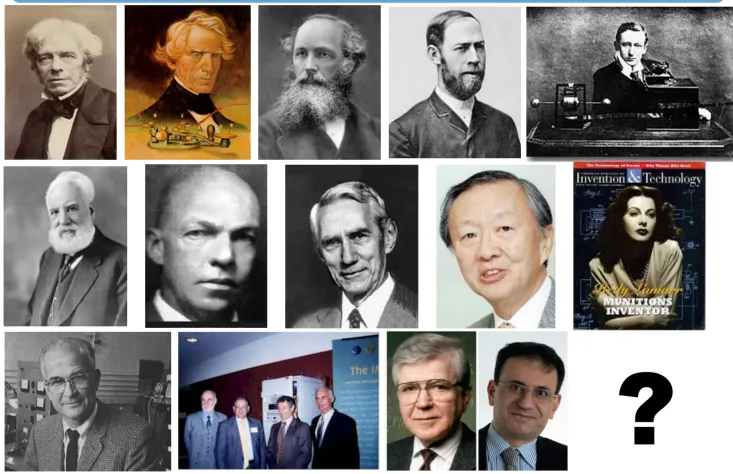
\includegraphics[width=0.8\textwidth]{../assets/ch01/ch01-1_0_通信网络简史-000.png}
\end{figure}
人、马和信鸽一直是古代用于信息传递的工具，容易获得，但相对效率不高。中国的烽火台通信是一个经过精心设计的通信系统。烽火台是万里长城防御工程中最为重要的组成部分之一。烽火台除了传递军情之外，还为来往使节保护安全、提供食宿、供应马匹粮秣等服务。烽火台在长城防御体系中的主要作用是作为传递军情的设施，有些地段的长城只设烽台而不筑墙。烽火台的设计要点包括：
\begin{figure}[htbp]
\centering
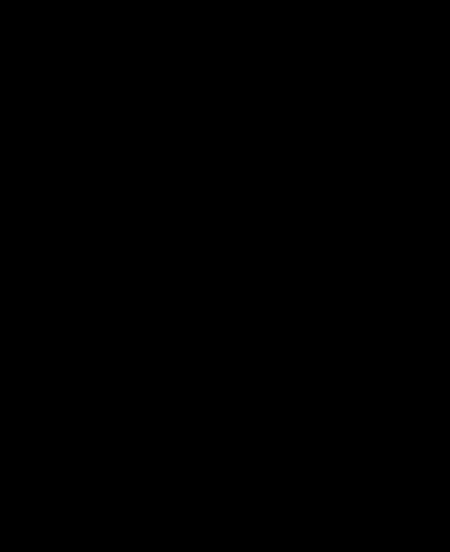
\includegraphics[width=0.8\textwidth]{../assets/ch01/ch01-1_0_通信网络简史-001.png}
\end{figure}
 ● 信号：因白天阳光很强，火光不易见到，夜间火光很远就能看见。传递信息的方法是白天燃烟，夜间举火。
 ● 信号量：通常会以为传递的信息是简单的二进制0/1表示方式。事实上，为了报告敌兵来犯的多少，采用了以燃烟、举火数目的多少来加以区别。此外，明朝还在燃烟、举火数目的同时加放炮声，以增强报警的效果，使军情传递顷刻千里。
 ● 可靠性：烽火台的布局也是十分重要的，要把它布置在高山险处或是峰回路转的地方，而且必须是别保障同时三个台都能相互望见，以便于发现和传递可靠。

近现代通信
1831年, 英国物理学家和化学家 法拉第
\begin{figure}[htbp]
\centering
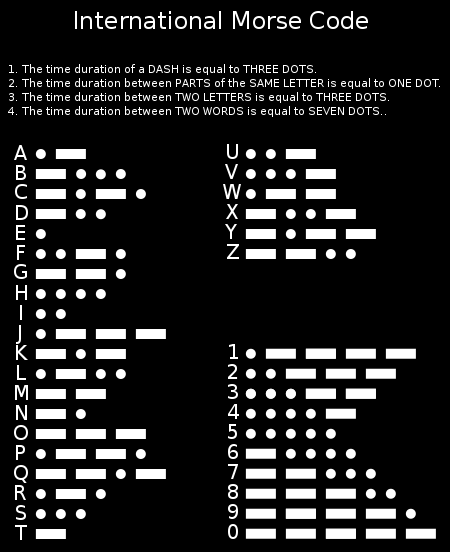
\includegraphics[width=0.8\textwidth]{../assets/ch01/ch01-1_0_通信网络简史-002.png}
\end{figure} Michael Faraday (1791-1867) 发现了电磁感应现象。英国物理学家和化学家，经典电磁理论的奠基人 麦克斯韦 James Clerk Maxwell (1831-1879) 创建并领导了英国第一个专门的特刊实验室——卡文迪许实验室。总结了19世纪中叶以前对电磁现象的研究成果，建立了电磁场的基本方程，即麦克斯韦方程组。从这一理论中得出，电磁过程在空间是以一定速度（相当于光速）传播的，并得出光的本质是电磁波的结论。1887年，赫兹 Heinrich Rudolf Hertz (1857-1894)用自己设计的振荡器，第一次通过实验证实了电磁波的存在。研究在空气中的传播速度等於光速，确立了电磁波和光波基本特性的同等性。首先发现了光电效应现象。为了纪念他，人们以赫兹作为振荡频率的单位。

\begin{figure}[htbp]
\centering
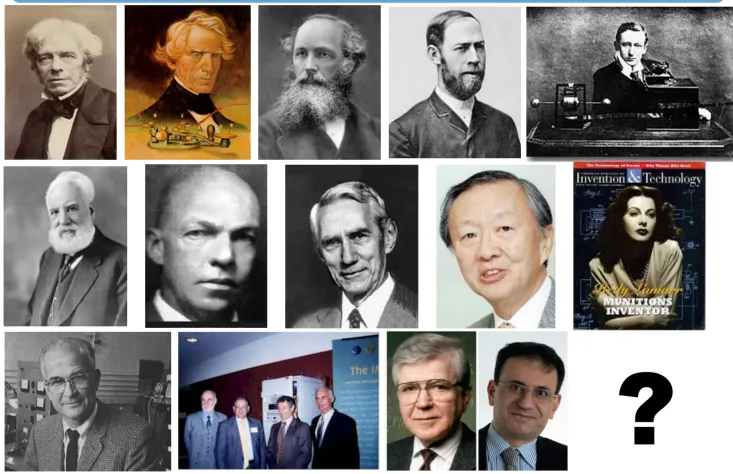
\includegraphics[width=0.9\textwidth]{../assets/ch01/ch01-1_0_通信网络简史-000.png}
\caption{通信发展史上的重要人物}
\end{figure}

根据电磁技术引入数据通信，人们陆续发明了电报(1837, Morse)、电话(1876 Bell)、无线电(1895Попов，Marconi )、卫星通信和网络（1950s）。从技术的观点上来看，电报实现了长距离即时通信，第一个实现了除人和货运之外的信息传输。从社会与文化的角度来看，全球电报网络的快速部署也表明快速可靠的通信是现代社会不可或缺的。因此我们首先了解电报，包括信息理论和长距离传输技术。
早在法国大革命期间（1800s），法国仍然使用类似烽火台的信号塔来传递信息，不同的是它使用机械臂来表示不同的字母。 信号塔的传输速度不够快，包括安培和高斯的很多科学家在尝试用电来传递信息。这里有两个主要的难题，一是如何表示信息；二是如何实现长距离传输。1837-1839年，英国人库克和惠斯通（William Cooke 和 Charles Wheatstone 最早使用电实现长距离通信的技术实现了历史上第一条电报线；1844年，莫尔斯 （Samuel Morse，1791-1872) 改进了传统电报机，研制出最早的电磁式电报机，创造了著名的点画组合莫尔斯电码，部署并推广电报系统。针对第一个问题，26个字母和10个数字符号使用36根线或者36种电的表达方式会导致系统非常复杂。如果方向错了，人越是努力，距离真理越远。当莫尔斯在多年劳心劳力劳财的设计复杂系统的过程中，意识到高速电信号只能表示简单的通断，通过不同的通断组合来表示信息。但这个过程中也没有一路畅通。莫尔斯早期也曾采用字典编码，即对每一个字典中的符号对应数字。但这种方法不够高效且不能覆盖字典中没有的词。 另一种编码方式就是对每一个字母进行编码，也就是我们常说的莫尔斯电码 （Morse Code）。值得注意的是，莫尔斯电码成功的另一个原因是由于其简单性，可以配套一个自动化的基于纸带点线的收发装置。

\begin{figure}[htbp]
\centering
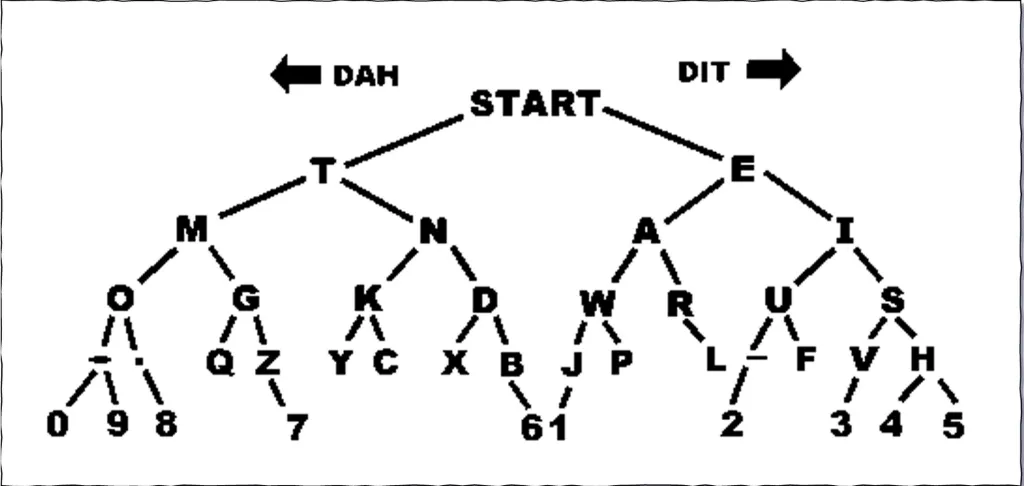
\includegraphics[width=0.8\textwidth]{../assets/ch01/ch01-1_0_通信网络简史-003.png}
\caption{莫尔斯电码树}
\end{figure}

莫尔斯电码本质上是一棵霍夫曼树
\begin{figure}[htbp]
\centering
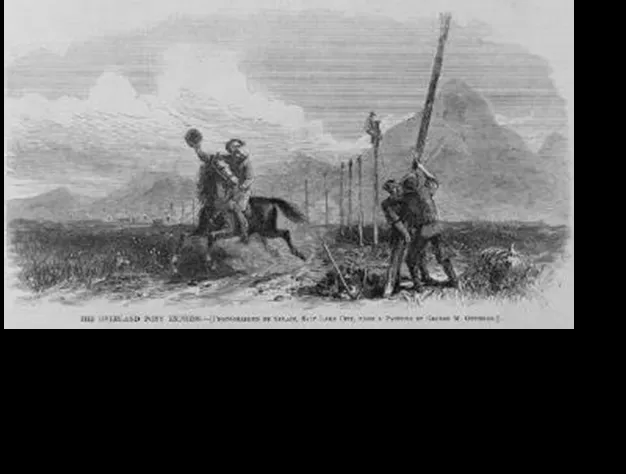
\includegraphics[width=0.8\textwidth]{../assets/ch01/ch01-1_0_通信网络简史-004.png}
\end{figure}，编码的规则是常用的字符点击次数少，并按照字符出现概率分配对应点击数量。例如T、E 出现频率最高，所以用一次点击电键的数量。
电报的长距离传输是另一个要解决的问题。当时的主要限制是没有发电机，主要依赖电池；铜导线纯度不高，电阻很大。针对第一个问题，纽约大学的Leonard Gale教授找到了关键点在于-电压不够，并通过电池串联，采用更大的电感线圈等方法提高传输距离到10英里。康奈尔大学的联合创办者Ezra Cornell发明了绝缘电缆，提高了传输过程中的信噪比。进一步，为实现城市间数据通信的问题，莫尔斯和同事一起，将长距离通信变成很多短距离通信，也就是利用电磁铁继电器来接力传输。
可见，技术的普及不能仅限于好的思想，还需要有好的系统支撑。以莫尔斯电码的普及为例，这个过程需要下面几个条件
 ● 设计高效的Morse code
 ● 实现简单实用的电报机
 ● 克服长距离传输的限制
 ● 主动推广业务以及获得资金和技术支持
电报第一次使以往彼此隔绝的世人能够同时获悉世界上发生的事。到了1850年，陆上电报已经遍布欧洲北美和中东。但是，那些对海洋隔离的国家依然处于没有电讯联系的状态。1851年英格兰连接到欧洲大陆通过英格兰和法国之间的一条电缆。这样连接欧洲和美洲的跨大西洋电缆
\begin{figure}[htbp]
\centering

\includegraphics[width=0.8\textwidth]{../assets/ch01/ch01-1_0_通信网络简史-005.png}
\end{figure}就题上了日程。1854年，美国富商塞勒斯.菲尔德（Cyrus West Field）萌生了一个更伟大的想法，为什么不能通过海底电缆在纽约和纽芬兰连接后也和爱尔兰联系起来呢？铺设横跨大西洋的海底电缆。当时的电缆技术仅支持短距离浅海敷设（最长177千米，深度550米），而跨大西洋电缆需跨越3200千米，最深达4750米。海水导电性引发的信号延迟、电缆材料强度不足、深海高压等问题均无先例可循，被比作"1957年人类未登月便计划探索月球"。

\begin{figure}[htbp]
\centering
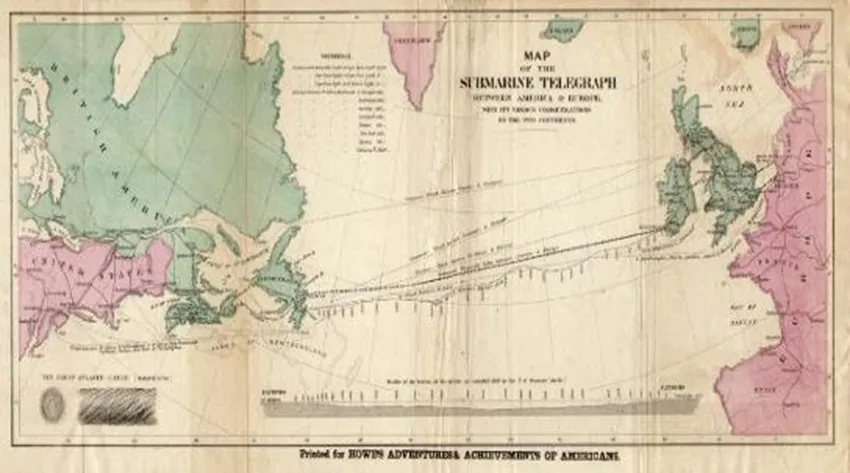
\includegraphics[width=0.9\textwidth]{../assets/ch01/ch01-1_0_通信网络简史-006.png}
\caption{跨大西洋电缆地图}
\end{figure}

 ● 1857 年，他第一次尝试从欧洲大陆出发把电缆铺设到大西洋中部，起航的第六个晚上意外发生了：电缆断了。就这样一个小小的技术差错毁掉了几年的筹备工作。
 ● 1858年，他进行了第二次尝试，可惜因暴风雨，电缆遭到严重的损坏。1858年有进行了第三次尝试，电缆终于铺设成功。一根电缆工作了一个月，由于高电压的传输问题，海底电缆断线了，北美再也接收不到欧洲传来的清晰的信号。一夜之间，菲尔德倾家荡产、身败名裂、朋友亲人纷纷离开，从举国狂欢到人人谩骂。之后发生的美国内战让新的尝试暂停下来。
 ● 1866年，在铺设横越大西洋电缆的计划沉寂了六年后，经过材料改良（采用古塔胶强化绝缘层）和工程优化，菲尔德购买了世界第一巨轮"伟大的东方人"号，重新开始，但在离北美还有两天航程的时候电缆突然断裂，这第四次尝试再次失败。。1866年7月13日，"伟大的东方人"号第二次出航，终获成功。数天以后，那条6年前沉睡的电缆被重新找到，使大西洋电缆成为双线，传输速度比1858年快50倍。这一成就被誉为"人类地理隔阂的终结"，直接推动19世纪末环球电报网络的形成。

\begin{figure}[htbp]
\centering
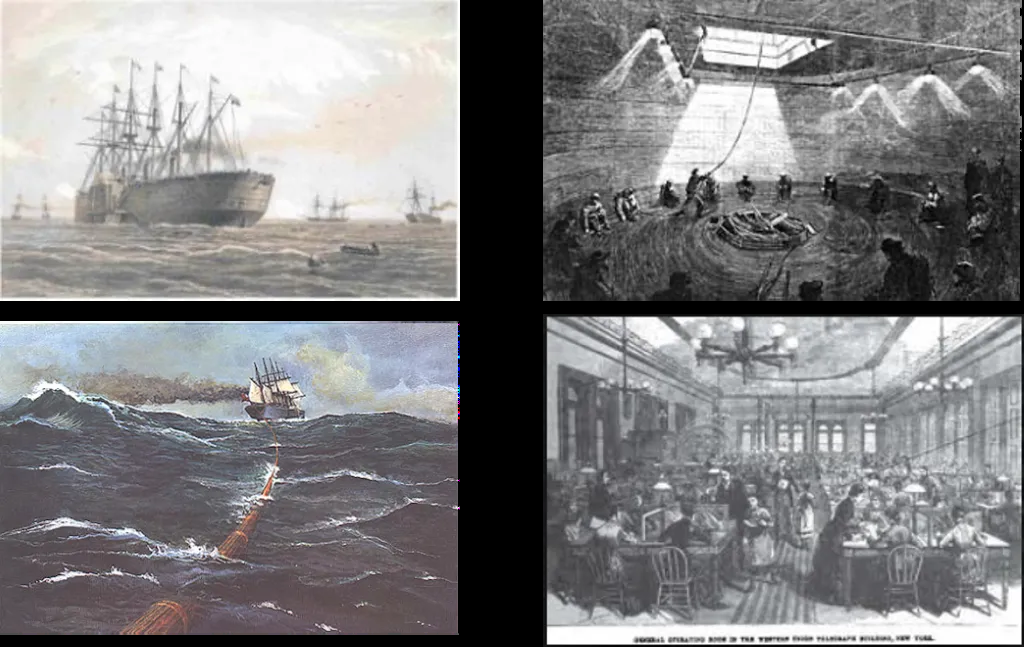
\includegraphics[width=0.9\textwidth]{../assets/ch01/ch01-1_0_通信网络简史-008.png}
\caption{跨大西洋电缆铺设过程}
\label{fig:transatlantic-cable}
\end{figure}

18世纪五十年代到六十年代，海底电缆铺设成为了当时最主要的工程项目。它促进了造船业、电缆制造，电子工程的发展。从工程技术的角度来说，海底电缆的主要技术难点是长距离信号传输，信号衰减和散射。散射影响长距离电缆的质量性能，一分钟只能传几个字符。威廉 汤姆森（William Thompson, later called Lord Kelvin） 首次研究了这一问题。他借鉴了傅里叶方程来从传输媒体中解调出信号，并设计了更高灵敏度的信号接收器，来解决这一问题。这个方法为之后电信和信号处理的工作奠定了理论基础。汤姆森在1893年芝加哥召开的国际电学大会上，提出了采用伏特、安培、法拉和欧姆等作为电学的基本单位，这些国际标准获得正式通过并被沿用至今在跨大西洋电缆的建设中，多位科学家提供了关键支持，推动了这一史诗级工程的实现。塞缪尔·摩尔斯（Samuel Morse）摩尔斯电码的发明者，也是美国陆上电报线路建设的先驱。当塞勒斯·菲尔德（Cyrus West Field）征求他的意见时，他热情支持了这一构想，为项目提供了技术信心。马修·方丹·莫里（Matthew Fontaine Maury）美国海洋学家和海军军官，他通过精确的海洋测绘数据，为菲尔德提供了纽芬兰岛到爱尔兰岛之间海底地形的详细信息。莫里认为两地之间的海底高原地形非常适合敷设电缆，这为工程选址提供了科学依据。此外，电报的发展也促进了新闻业的发展。例如，路透社即是通过海底电报线在德国和英国见交换股市信息发展起来的。

电话是另一个在通信领域的里程碑的技术
\begin{figure}[htbp]
\centering
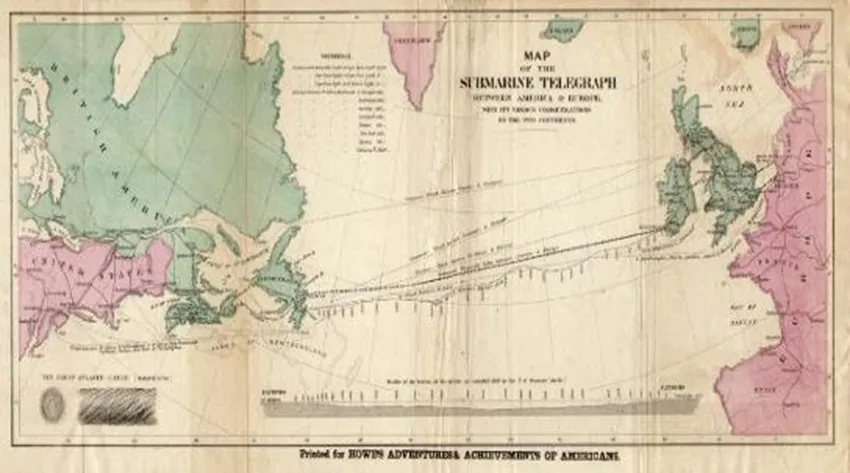
\includegraphics[width=0.8\textwidth]{../assets/ch01/ch01-1_0_通信网络简史-006.png}
\end{figure}。它可以看成是电报电缆性能的直接扩展。1860年，意大利人穆奇向公众展示电话的原型。1870年后，一系列电子工程师包括托马斯爱迪生，实现了可以在同一根电报线上同时传输多路电报信号的可靠系统。同时，更多的工程师们开始探索调谐电报，也就是用不同的音调来同时传输多路离散的电报信号。美国的贝尔(Alexander Graham Bell 1847-1922，来自苏格兰的聋哑人教师) 和格雷（Elisha Gray）几乎同时意识到一跟电话线可以传输话音信号。1875年，贝尔 1876年3月10日，通过电报线路通话成功，助手沃特森通过液体发射机和调谐舌簧接收机第一次听到了贝尔发来的声音。在1876年早些时候，贝尔很幸运的比格雷早了几个小时签署了一份专利。电话业务很快的实现了本地服务。1878年，贝尔和合作者在相距300公里的波士顿和纽约之间成功进行了长途电话的公开实验，创办了贝尔电话公司，推动了电话的迅速发展。同期，磁石电话和人工电话交换机（注：和当前使用的网络交换机并不相同）诞生。1880年，发明了供电式电话机，贝尔公司也已经卖出了10,000台机器。1880年，世界上第一本黄页电话号簿在美国问世。1892年，发明了步进式自动电话交换机（1898年，戊戌变法开始并迅速失败。 1871年，第一条电报线路 （1844年美国第一条电报线路）1881年，天津至上海电报服务（洋务运动）。1884年，北京民用电报业务。1895年，李鸿章在日本通过电报与清廷进行密电联络，因为泄密，导致谈判被动，签下《马关条约》。21世纪初，电报业务逐渐退出历史舞台）。

\begin{figure}[htbp]
\centering
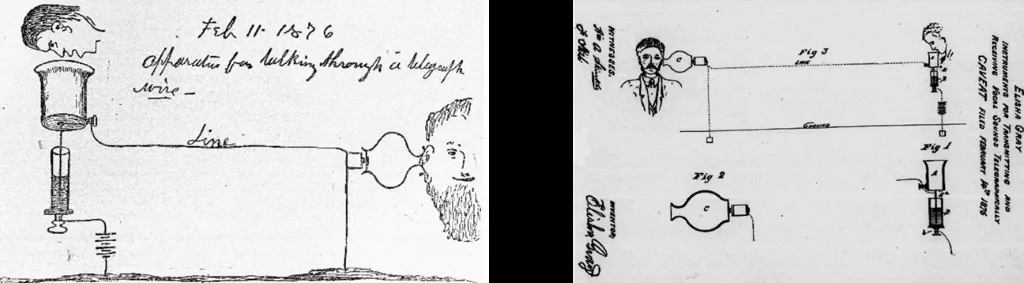
\includegraphics[width=0.9\textwidth]{../assets/ch01/ch01-1_0_通信网络简史-010.png}
\caption{贝尔的电话专利图}
\end{figure}

\begin{figure}[htbp]
\centering
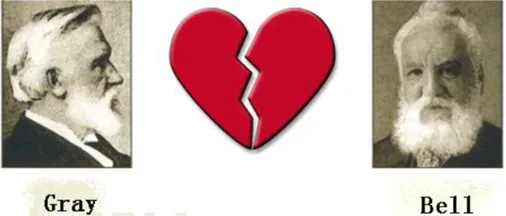
\includegraphics[width=0.6\textwidth]{../assets/ch01/ch01-1_0_通信网络简史-012.png}
\caption{格雷与贝尔的专利之争}
\end{figure}

早期电话的两个主要问题是 交换和长距离传输。首先，电话需要接线员手动接线。但是，这样做会非常慢而且很累。1889年，A.B.Strowger (堪萨斯城的火葬场老板) 获得了自动拨号系统的专利。这个系统相当成功，1892年开始部署并一直在使用到1970s. 其次，长距离传输是一个很困难的问题，需要数十年的研究和开发。和水下电缆的长距离传输类似，信号的衰减和散射导致电话信号随着距离增加飞快衰减。一对铜缆可以传输100英里话务，但是超过这个距离，用户已经不能够理解收到的话音信号了。成功的长距离电话信号传输需要两个技术突破：Inductive loading和Amplification。这种公司组织的研发的开创性方法也许是长距离电话通讯的最重要遗产。

\begin{figure}[htbp]
\centering
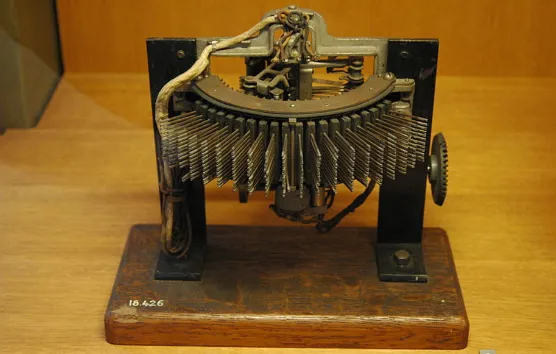
\includegraphics[width=0.6\textwidth]{../assets/ch01/ch01-1_0_通信网络简史-016.png}
\caption{步进式自动电话交换机}
\end{figure}

1885年 贝尔电话公司
\begin{figure}[htbp]
\centering
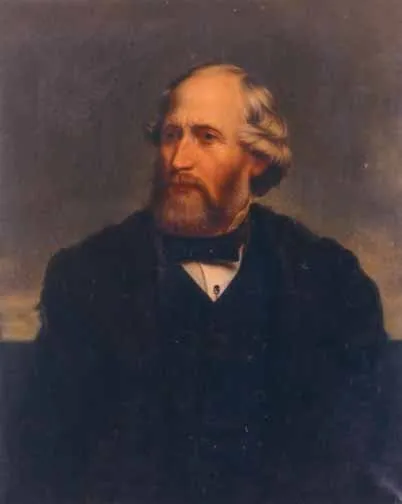
\includegraphics[width=0.8\textwidth]{../assets/ch01/ch01-1_0_通信网络简史-007.png}
\end{figure}长途业务部 AT&T。1900年 AT&T George Campbell 和哥伦比亚大学的Michael Pupin撰写了inductive loading 电话线的方法。AT&T买了这个专利，一次性付费185000美元并在17年的专利期内每年付费15000美元。这项技术确保了可以在纽约和Denver运营一个4300公里的电话线路。 另一方面，这也是没有放大器的话音信号传输的极限。英国科学家Fleming发明了二极管，美国的Lee de Forest在此基础上发明了三极管，成为了放大器和振荡器的重要组件。这样，在几年内，电子放大器就稳定的应用于电话系统。1915年AT&T铺设了纽约到旧金山的长途电话线路。从另一方面来讲，长话业务促进了AT&T的发展和长期研发投入。AT&T成立的贝尔实验室在电子工程和物理领域引领了科技发展， 例如负反馈，active filuters，控制论，载波传输系统，半导体电子，信息论等等。
无线通信是电子工程的发展催生的另一个伟大的通信技术。我们很难也不应该把无线电的发明归结到某一个人身上。 无线电可以追溯到1860s英国物理学家Maxwell。直到1888年，麦克斯韦方程仍只是一个优雅的数学公式。德国人赫兹在实验室真正检测到电磁感应现象，捕捉到了电磁波。另一个研究者Nikola Tesla（塞尔维亚、美国）实验了无线电并预测其作为长距离通信的用处。俄罗斯科学家Popov 研制灵敏度非常高的无线讯号接收机并于1890s中期给出了50km无线通信的演示。当波波夫表演无线电收报机后的1896年，22岁的爱尔兰-意大利裔科学家马可尼(Guglielmo Marconi 1874-1937)发明火花隙无线电发报机并展示自己的长距离无线电接收机。在1901年12月，马可尼实现了跨大西洋远距离无线电通信，在加拿大纽芬兰收到来自英国的无线信号，开辟了无线电远距离通信的新时代，并于1908年获得诺贝尔奖。
早期的无线电设备大而笨重
\begin{figure}[htbp]
\centering
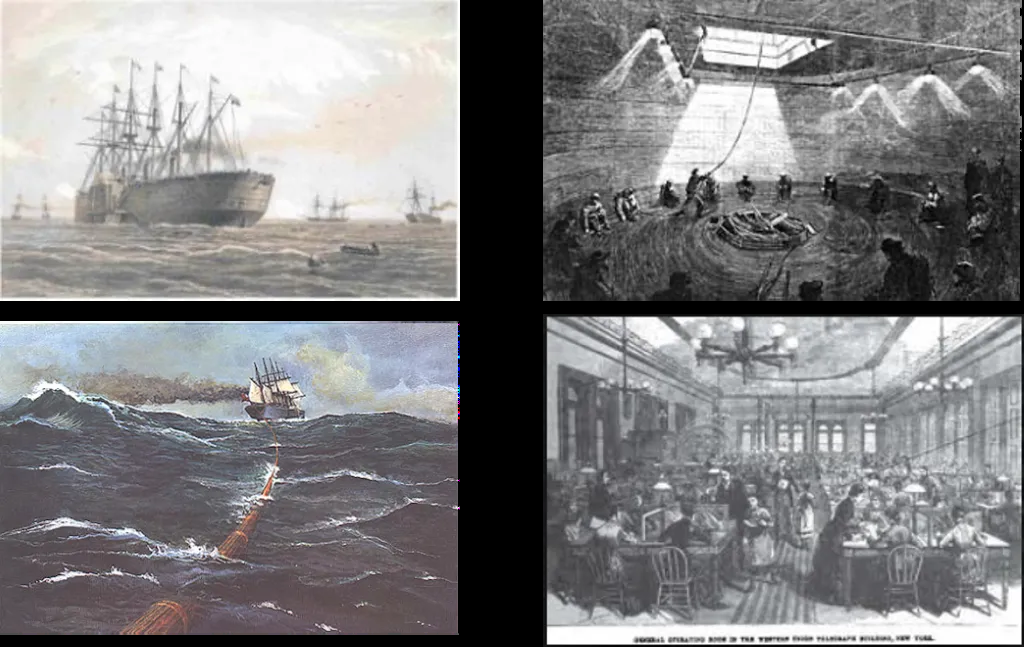
\includegraphics[width=0.8\textwidth]{../assets/ch01/ch01-1_0_通信网络简史-008.png}
\end{figure}，很难做精确的调节，而且多个发送机会造成干扰。感谢1908年Lee de Forest发明的三极管，使得精准的无线信号传送和接收成为可能。Edwin Howard Armstrong（哥伦比亚大学电感负载发明人Pupping的学生，FM发明人），可能是二十世纪最棒的电子工程师，利用三极管设计了震荡电路。可以用一个固定的频率发送连续的电磁波，并利用放大电路提高了接收器的调协能力和灵敏度。
直到1920年，无线电技术的主要应用都是无线电报
\begin{figure}[htbp]
\centering
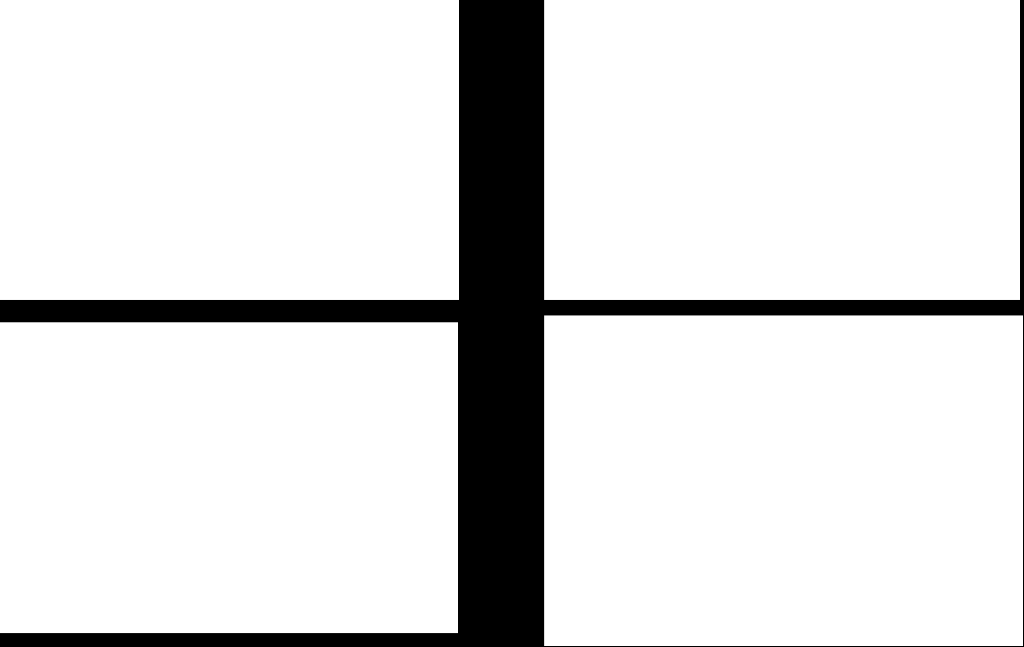
\includegraphics[width=0.8\textwidth]{../assets/ch01/ch01-1_0_通信网络简史-009.png}
\end{figure}。20世纪初，三个重要的历史事件证明了它的重要性。其中最著名的是1912年4月份的泰坦尼克号事件。当巨轮泰坦尼克号撞上冰山的时候，它发出了"SOS"的信号求救，但是没有船只及时赶来救援，因为当时很少有船安装无线接收设备（radio watch）。最终2200名乘客和船员，仅有700人幸存。 仅仅一年半之后，客轮Volturno号在大西洋起火，但此次，有10艘安装了无线接收设备的船只迅速赶到，所有人最终获救。所以如果无线工程师们的进度再快一点，电影《泰坦尼克号》就可能是个喜剧结尾。之后，无线电广播开始流行，1916年 Frank Conrad，一个业余的无线电发烧友，开始在匹兹堡的家里广播音乐。Westinghouse 这家公司意识到无线电广播具有巨大的市场，在1920年11月建立了世界第一个商用广播电台，KDKA。1923年在美国就有超过500个电台。在欧洲BBC在1932年成立。1940年Armstrong建立了FM广播网络使用42-50Mhz频段。

\begin{figure}[htbp]
\centering
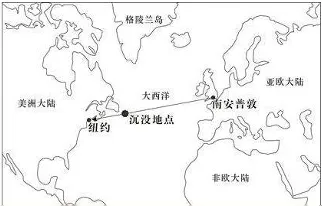
\includegraphics[width=0.9\textwidth]{../assets/ch01/ch01-1_0_通信网络简史-019.png}
\caption{Titanic号失事地点}
\end{figure}

第二次世界大战，促成了雷达技术的发展
\begin{figure}[htbp]
\centering
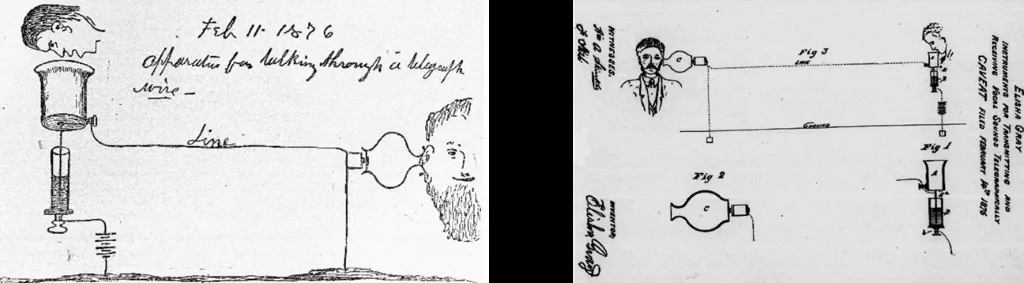
\includegraphics[width=0.8\textwidth]{../assets/ch01/ch01-1_0_通信网络简史-010.png}
\end{figure}。1935年英国物理学家Sir Robert Watson-Watt设计了（introduced）第一套实用雷达装置。1939年英国军队建立了"chain home"雷达站网络来检测天空和海上的入侵者。1940年9月，英国军方决定和美国共享雷达技术。美国在MIT建立了放射实验室（Radiation Laboratory）。雷达证明对盟军非常重要，到1943年盟军实用雷达作为早期预警、战场指挥、空中搜索、夜间袭击、轰炸和高射炮瞄准。战时雷达研究促成了和平时期的红利，如电视、FM、VHF和微波通信，全天候的航空航海，甚至家用的微波炉也是使用谐振腔式磁控管来加热食物。
1948年有两个主要的进展：
1. Shockley，Bardeen 和Brattain发明晶体管；
2. Claude Shannon发表了具有重大意义的"A Mathematical Theory of Communication"。四个人都在贝尔实验室。这两个先进发展促进了一系列技术发展，包括电话水下电缆，通信卫星，数字和数据通信。（这期间，控制论也获得了重要发展 《Cybernetics: Or the Control and Communication in the Animal and the Machine》, Norbert Wiener 1894-1964）

\begin{figure}[htbp]
\centering
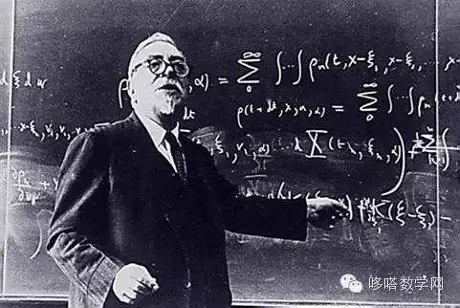
\includegraphics[width=0.8\textwidth]{../assets/ch01/ch01-1_0_通信网络简史-023.png}
\caption{Norbert Wiener与控制论}
\end{figure}

威廉·肖克利（William Shockley）
\begin{figure}[htbp]
\centering
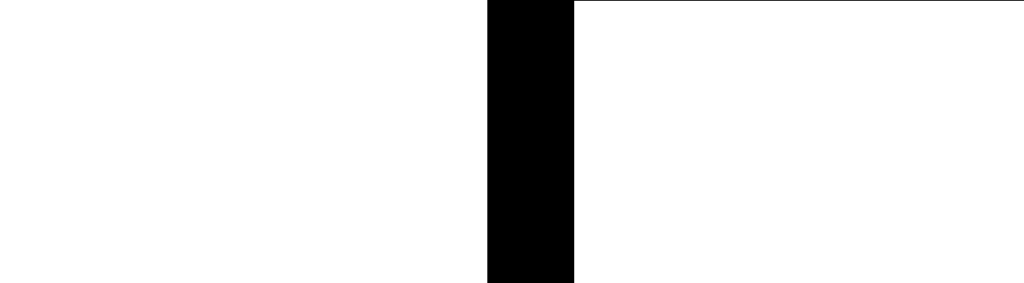
\includegraphics[width=0.8\textwidth]{../assets/ch01/ch01-1_0_通信网络简史-011.png}
\end{figure}是20世纪最重要的物理学家之一，被誉为"晶体管之父"。他于1910年2月13日出生于英国伦敦，后移居美国，并在加州理工学院和麻省理工学院获得学位。1936年，他加入贝尔实验室，开启了其改变世界的科学旅程。1947年12月16日，肖克利与约翰·巴丁（John Bardeen）和沃特·布拉顿（Walter Brattain）在贝尔实验室成功制造出第一个点接触式晶体管，这一发明被誉为"20世纪最重要的发明"之一。晶体管是一种能够放大和控制电流的半导体器件，它取代了笨重且低效的真空管，为现代电子技术的发展奠定了基础。1948年，肖克利进一步提出了双极性结型晶体管（BJT）的理论，这一设计比点接触式晶体管更实用，成为晶体管技术的主流。1956年，肖克利、巴丁和布拉顿因晶体管的发明共同荣获诺贝尔物理学奖。

\begin{figure}[htbp]
\centering
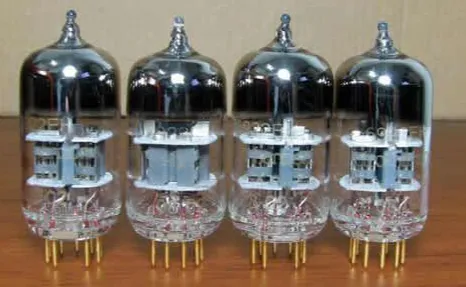
\includegraphics[width=0.9\textwidth]{../assets/ch01/ch01-1_0_通信网络简史-025.png}
\caption{电子管}
\end{figure}

\begin{figure}[htbp]
\centering
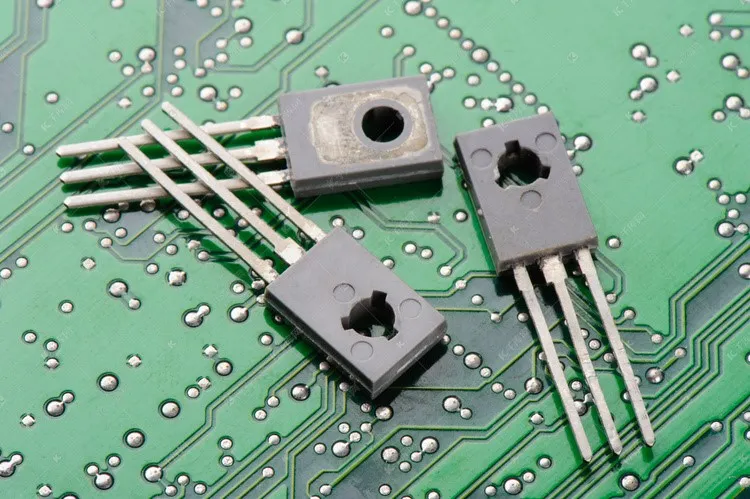
\includegraphics[width=0.9\textwidth]{../assets/ch01/ch01-1_0_通信网络简史-026.png}
\caption{晶体管}
\end{figure}

\begin{figure}[htbp]
\centering
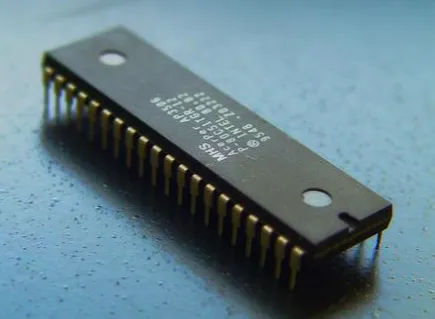
\includegraphics[width=0.8\textwidth]{../assets/ch01/ch01-1_0_通信网络简史-027.png}
\caption{集成电路}
\end{figure}

克劳德·香农（Claude Shannon）
\begin{figure}[htbp]
\centering
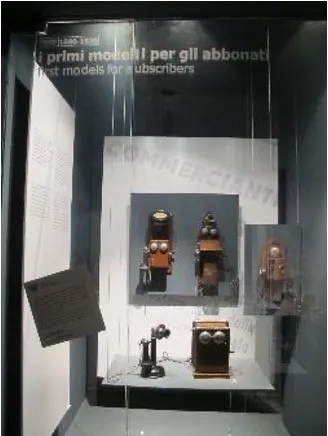
\includegraphics[width=0.8\textwidth]{../assets/ch01/ch01-1_0_通信网络简史-014.png}
\end{figure}"信息学之父"。1936年，香农从密歇根大学获得数学和电子工程双学士学位，随后进入麻省理工学院（MIT）深造。1938年，他发表了硕士论文《继电器与开关电路的符号分析》，首次将布尔代数应用于电路设计，为数字计算机的发展奠定了理论基础。这篇论文被誉为"有史以来最重要的硕士论文"。1948年，香农在《贝尔系统技术杂志》上发表了划时代的论文《通信的数学理论》，标志着信息论的诞生。他提出了信息熵的概念，定义了信息量的数学表达式，并解决了信道容量、信源编码等一系列核心问题。这篇论文被称为"信息时代的大宪章"，为现代通信技术提供了理论基础。二战期间，香农在贝尔实验室从事密码学研究，负责追踪纳粹德国的飞机和火箭。他还参与了罗斯福和丘吉尔之间的绝密跨大西洋电话线的安全设计。1945年，他提交了《密码学的一个数学理论》，为现代密码学奠定了基础。2001年2月24日香农去世，享年84岁。为纪念他的贡献，通信理论领域的最高奖项被命名为"香农奖。

\begin{figure}[htbp]
\centering
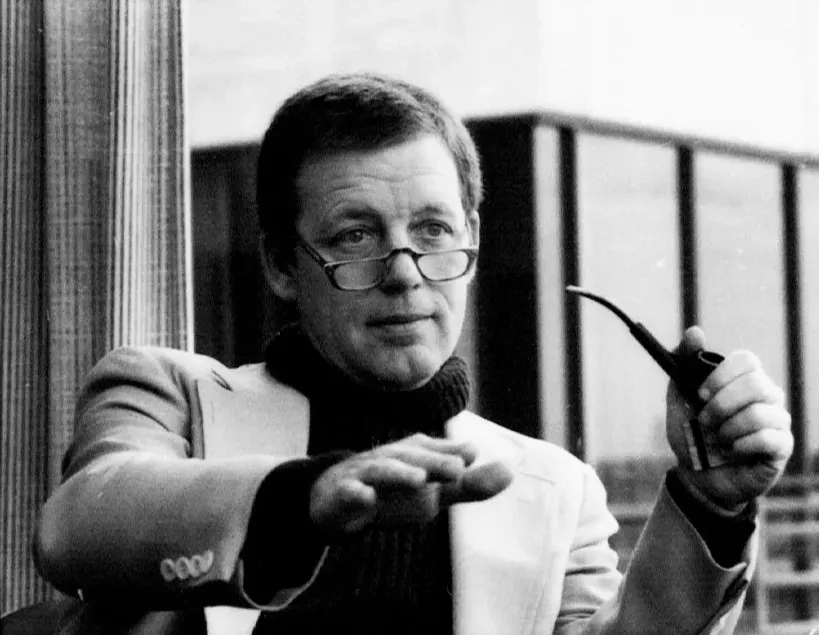
\includegraphics[width=0.6\textwidth]{../assets/ch01/ch01-1_0_通信网络简史-029.png}
\caption{Claude Shannon}
\end{figure}

数据通信也在这段时间发展起来
\begin{figure}[htbp]
\centering
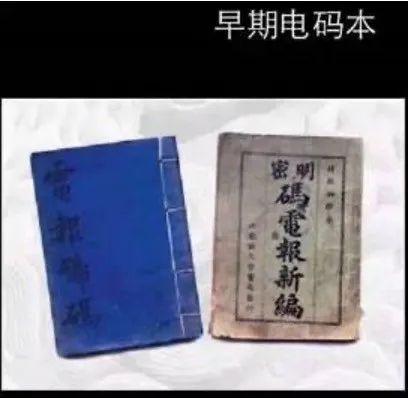
\includegraphics[width=0.8\textwidth]{../assets/ch01/ch01-1_0_通信网络简史-015.png}
\end{figure}。一些有趣的历史事件包括：
 ● 1946年，世界上第一台电子计算机ENIAC诞生。
 ● 1949年，美国空军资助了计算机电子防御网（computerized electronic defense network）SAGE（Semi-atutomatic electronic defense network），通过协调雷达站和防空系统来拦截轰炸机。SAGE后来促进了第一个大规模的商用计算机网络。
 ● 1955年，肖克利离开贝尔实验室，在加州山景城创立了肖克利半导体实验室。他招募了一批优秀的年轻工程师，包括后来被称为"八叛逆"的戈登·摩尔（Gordon Moore）和罗伯特·诺伊斯（Robert Noyce）等人。1957年9月18日，肖克莱半导体实验室开发部门的"八大金刚"（"八叛徒"）集体辞职，在仙童（Fairchild）照相器材公司的资助下创办了仙童半导体公司。
 ● 1958年，发明集成电路（IC）
\begin{figure}[htbp]
\centering
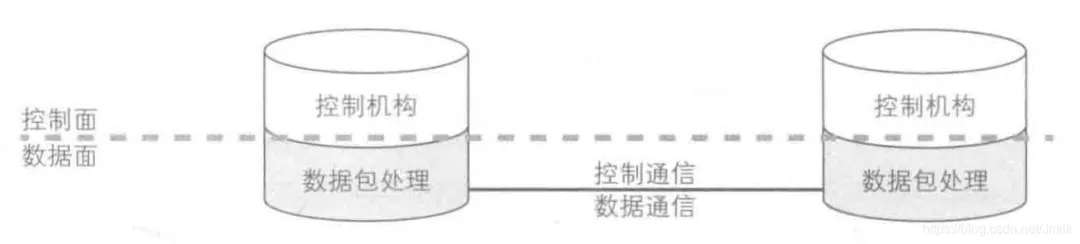
\includegraphics[width=0.8\textwidth]{../assets/ch01/ch01-1_0_通信网络简史-043.png}
\end{figure}。杰克·基尔比（Jack Kilby）在德州仪器（Texas Instruments）工作时，提出了将多个电子元件集成在一块半导体材料上的构想，成功在一块锗片上集成了晶体管、电阻和电容，并用细金线连接。基尔比的发明证明了集成电路的可行性，并于2000年获得诺贝尔物理学奖。罗伯特·诺伊斯（Robert Noyce）采用平面工艺（Planar Process），在硅片上制造集成电路，并使用铝金属线实现元件之间的连接。这一方法更易于大规模生产，成为现代集成电路制造的基础。 台积电的张忠谋和基尔比曾经共事过，见证了他发明集成电路的过程。
 ● 1961年，Bell System使用T1承载网发送数字话音信号。该系统使用了由1938年英国工程师Alec Reeves发明的PCM编码。
 ● 1964年SABRE 航空订票系统由IBM为美国航空建设。这套系统使用modem在普通模拟电话线传输数字信号，速率1200b/s。使用modem的发送数据的方法获得广泛使用。
1956年，Bell System 和 British Post Office发起了跨大西洋话务电缆TAT-1。这个时间，水下电报电缆已经服务超过100年。电话也使用了80年了。然而，在安装TAT-1之前，长距离电缆的散射和衰减仍然导致不能传输能听得懂的话音。TAT-1能够传输36路4KHz通道，TAT-1一直使用到1979年。还有一些电缆也相继建设，例如：法国和纽芬兰（TAT-2），阿拉斯加和华盛顿洲，夏威夷到加州。这期间的技术发展包括：
  ● 1956年和1960s初期，频谱效率提高从4KHz到3KHz。
  ● 1959年引入Time Assignment Speech Interpolation（TASI）-- 语音插空系统 （利用语言间歇的电路时间交错分割多路通信制。TASI是电路复用系统提高电话线的传输能力。它根据这样的事实，一般的通话过程中实际通话时间只占用电话时长的40%。通过使用快速交换和话音检测器，该系统允许时间复用。Bell的工程师为长话电缆开发了固态电路（Solid-State Circuitry），晶体管放大电路并在1963年后即开始部署。

\begin{figure}[htbp]
\centering
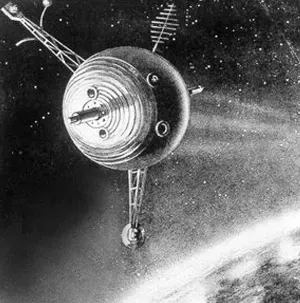
\includegraphics[width=0.6\textwidth]{../assets/ch01/ch01-1_0_通信网络简史-028.png}
\caption{人造卫星}
\end{figure}

卫星通信是另一个重要的长距离通信的方向
\begin{figure}[htbp]
\centering
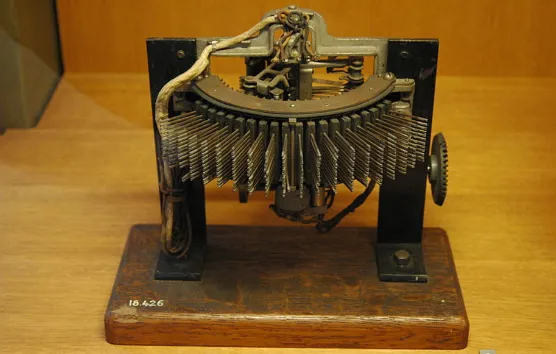
\includegraphics[width=0.8\textwidth]{../assets/ch01/ch01-1_0_通信网络简史-016.png}
\end{figure}。第二次世界大战期间和之后微波电路的发展，特别是波导和谐振腔能够处理大到100GHz，使得卫星通信成为可能。美国和苏联（U.S.S.R）的空间项目开始于1950s中期。1957年10月4日苏联发射了第一个人造卫星，Sputnik。4个月后美国的卫星Explorer I送上轨道。值得注意的是，1958 年 2 月美国国防部组建了 APRA（Advanced Research Project Agency，美国国防部高级研究计划局）科研部门。ARPA 的主要工作，就是研究如何将那些具有潜在军事价值的 "黑科技"，应用于军事领域，包括弹道导弹防御、卫星导航、核试验检测等等。。 1960s，第一个商用卫星，被动反射式 Echo I，被发射到中高度轨道，证实了跨大西洋卫星通信的可能性。被动卫星的缺点是需要非常高的传输功率来克服路径损耗。因此，通信工程师们开始开发可以接收重传信号的主动式卫星。1962年7月，Telstar I世界上第一个主动卫星发射。工程师在英国建立了第一个抛物线天线和卫星建立连接。但是，没有预期到的范艾伦辐射带产生的辐射使它只工作了几个星期。范艾伦辐射带是一个高能带电粒子带，其中大部分微粒来自于太阳风暴和宇宙射线，它们被地球周围的磁场捕获而形成了一条带状区域环绕地球。之后，做了更多防辐射处理的Telstar 2，在1963年5月7日发射，承载了1条电视通道4条电话通道。Telstar是一个实验项目而非商用系统。它表明卫星通信的可能性和可行性。1964年，一个包含100国家代表卫星通信国际推介和合作组织Intelsat成立。同年，第一个地球同步轨道商用卫星Syncom 3发射。

当代通信 -- Internet 诞生
\begin{figure}[htbp]
\centering

\includegraphics[width=0.8\textwidth]{../assets/ch01/ch01-1_0_通信网络简史-017.png}
\end{figure}
互联网（Internet）始于20世纪60年代，最初是为了让政府研究人员能够共享信息。当时，计算机体积庞大且无法移动，为了使用存储在任何一台计算机中的信息，人们要么需要亲自前往该计算机所在的地点，要么需要通过传统的邮政系统邮寄磁带。冷战的升级也是互联网形成的重要推动力。苏联发射的"Sputnik"卫星促使美国国防部思考在核攻击后如何继续传播信息。这最终促成了ARPANET（高级研究计划局网络）的诞生，该网络最终演变为我们现在所知的互联网。尽管ARPANET非常成功，但其成员资格仅限于与国防部有合同的特定学术和研究机构。为了应对这一限制，其他网络被创建以实现信息共享。1983年1月1日被认为是互联网的正式诞生日。在此之前的计算机网络之间没有统一的通信标准。一种新的通信协议，传输控制协议/互联网协议（TCP/IP），应运而生。这一协议使不同网络上的各种计算机能够"交流"。1983年1月1日，ARPANET和国防数据网正式切换到TCP/IP标准，互联网由此诞生。所有网络现在都可以通过一种通用语言连接在一起。
从技术的角度来说。1960s早期
\begin{figure}[htbp]
\centering
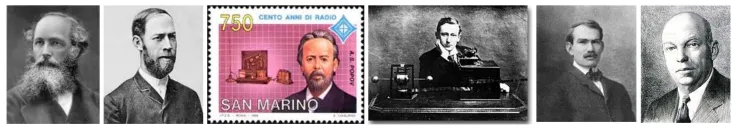
\includegraphics[width=0.8\textwidth]{../assets/ch01/ch01-1_0_通信网络简史-018.png}
\end{figure}，许多研究者意识到传统电路交换对于计算机通信效率过低。
 ● Paul Baran，兰德公司(Rand Corp.)的工程师开始考虑如何构建可以在第一波核打击下存活的通信网络（1961年，已经拥有核武器的苏联发射R-16洲际导弹），这种分布式通信系统同时也是APRA的核心项目之一 。1960年，Baran描述了"分布式通信"的技术。每个通信节点可以连接到多个其他通信节点。交换技术也是全网分布式的，给网络提供高度的可存活性。为了在网络中传输数据，Baran采用了分组交换技术。通过将信息数字化，切分成1024比特长数据包并附加一个包含路由信息的数据包头来传递数据，并在接收端重建。1964年Baran提出了无链接操作寻址技术（分组交换），目的是在战争残存的通信网中，不考虑时延限制，尽可能可靠地传递数据报。他在Rand期刊撰文"On Distributed Communications"介绍了系统的细节。
 ● 1961 年 5 月 ， Leonard Kleinrock 在 MIT 提 交 了 博 士 论 文 "Information Flow in Large Communicaiton Nets"。他提出"分组交换"概念，成功的在存储转发网络使用排队论，为因特网奠定了最重要的技术基础。同时，英国的Donald Watts Davies独立的开发了类似于Baran的系统，并创造了"packet"和"packet switching"概念来描述数据块和消息处理协议。
1966 年，来自 NASA（美国航空航天局）的罗伯特·泰勒（Robert Taylor）作为作为Internet前身"阿帕网"（ARPANet）的负责人，招揽了
 ● 美国加州大学洛杉矶分校（UCLA）的分组交换理论专家伦纳德.克兰罗克（L.Kleinrock）；
 ● 提出 "分布式通信理论" 的兰德公司科学家保罗.巴兰（P.Baran）；
 ● 麻省理工学院（MIT）林肯实验室的拉里·罗伯茨（Lawrence G. Roberts）；
拉里·罗伯茨则被任命为
\begin{figure}[htbp]
\centering
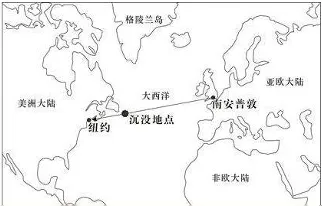
\includegraphics[width=0.8\textwidth]{../assets/ch01/ch01-1_0_通信网络简史-019.png}
\end{figure} ARPANET 项目的项目经理和首席架构师。1967 年 4 月，在美国密歇根州安娜堡召开的 ARPA IPTO PI 会议上，拉里·罗伯茨组织了有关 ARPANET 设计方案的讨论。不久后 就 发 表 第 一 篇 关 于 ARPANET 设 计 的 论 文 《 Multiple Computer Networks and Intercomputer Communication》（多计算机网络和计算机之间的通信）为阿帕网选择了"分组交换"通讯方式。在这样的项目中采用不成熟的分组交换而不是改进电路交换技术，需要远见和很大的勇气。非常多的ARPANET的先驱回忆分组交换遇到了通信工程师大量的抵抗和质疑。

\begin{figure}[htbp]
\centering
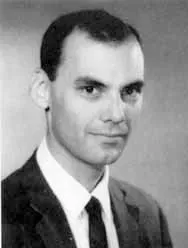
\includegraphics[width=0.9\textwidth]{../assets/ch01/ch01-1_0_通信网络简史-030.png}
\caption{罗伯特·泰勒（Robert Taylor）与拉里·罗伯茨}
\end{figure}

在罗伯茨的设计中
\begin{figure}[htbp]
\centering

\includegraphics[width=0.8\textwidth]{../assets/ch01/ch01-1_0_通信网络简史-020.png}
\end{figure}，主机不应该处理数据路由的任务，这个任务应该有一个小型的廉价计算机来承担，命名为 IMP（Interface Message Processor，接口信号处理机）。IMP 的作用是连接、调度和管理。主机把数据包发给 IMP，IMP 查看目标地址，或者把它传递到本地连接的主机，或者传递给另外一个 IMP。有了它，大型主机就不必 "亲自" 参与联网，从根本上解决了计算机系统不兼容的问题。后来，人们普遍将 IMP 视为路由器的雏形。为了防止数据包丢失，Sender IMP 会暂存数据包，直到获得 Receiver IMP 的 ACK 确认为止，如果没能收到确认，它就重新发送。在那时，ACK 重传机制还是由中间路由节点来完成的，后面才逐步演进到由主机 TCP/IP 协议栈来完成。

\begin{figure}[htbp]
\centering
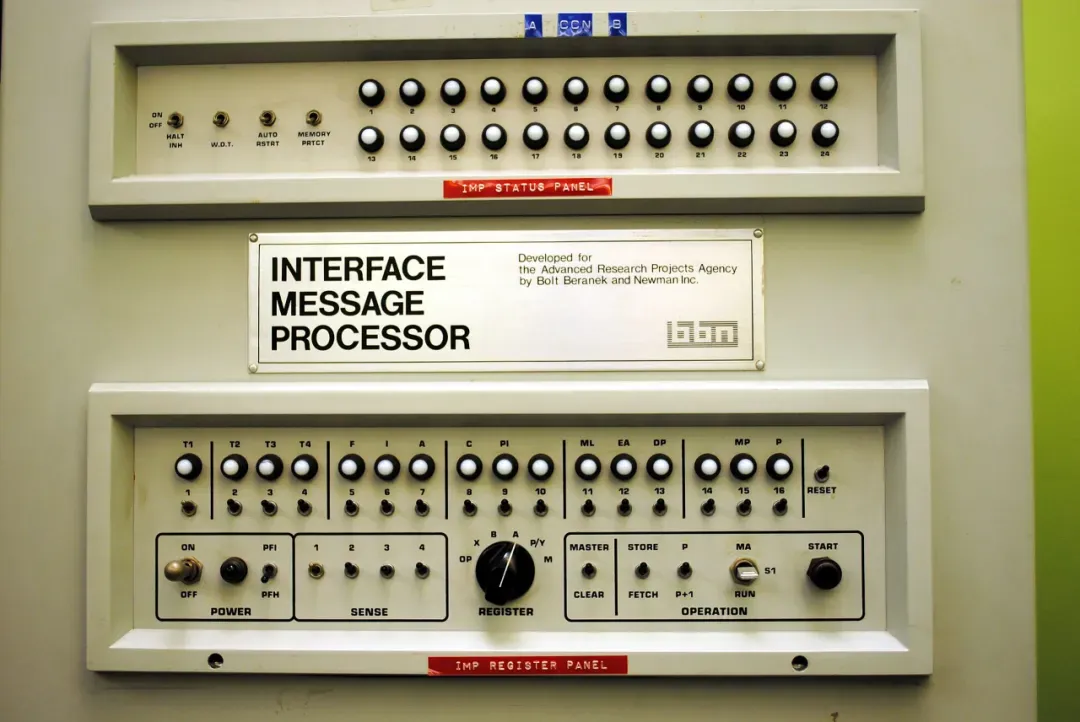
\includegraphics[width=0.9\textwidth]{../assets/ch01/ch01-1_0_通信网络简史-032.png}
\caption{IMP 设备面板}
\end{figure}

\begin{figure}[htbp]
\centering
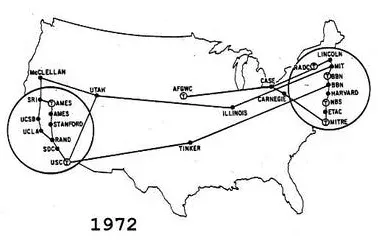
\includegraphics[width=0.9\textwidth]{../assets/ch01/ch01-1_0_通信网络简史-035.png}
\caption{IMP 设备内部}
\end{figure}

1969年，第一个 ARPANET诞生
\begin{figure}[htbp]
\centering
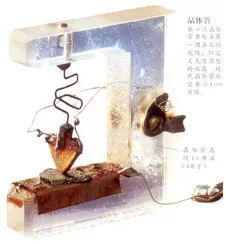
\includegraphics[width=0.8\textwidth]{../assets/ch01/ch01-1_0_通信网络简史-021.png}
\end{figure}，它连接了4所大学的4台大型计算机（加州大学洛杉矶分校、斯坦福大学研究学院、加州大学圣巴巴拉分校和犹他州大学的 4 台大型计算机）。

\begin{figure}[htbp]
\centering
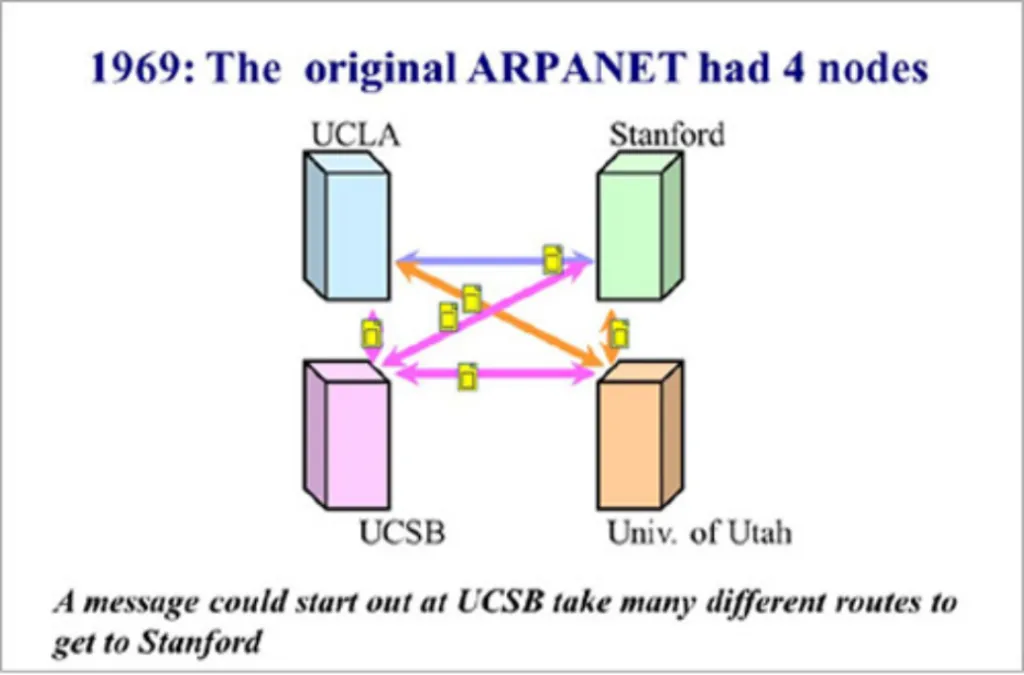
\includegraphics[width=0.8\textwidth]{../assets/ch01/ch01-1_0_通信网络简史-033.png}
\caption{ARPANET最初的4个节点}
\end{figure}

1970 年 12 月，通过软件的方式实现了最初的 ARPANET 通信协议，称为 NCP（网络控制协议），即网络通讯最初的标准。设计统一识别的信号来作为开通和关闭通信管道，否则这些 IMP 不会知道什么时候应该接收信号，什么时候该结束。1972 年，鲍伯·卡恩（Rober Kahn）在国际计算机通信大会（ICCC）上成功演示了 ARPANET 网络，那是 ARPANET 的首次公开亮相。经过几年的发展，在当年 ARPANET 已经拥有了 40 个节点，E-mail、FTP 和 Telnet 是当时最主要的网络应用。尤其是 E-mail，占据了 75% 的流量。在 ARPANET 成功的激励下，计算机网络领域开始渐渐出现了其他的一些网络类型，例如：夏威夷建立了 ALOHA 无线电网络，硅谷发明了以太网络，太空卫星也组建了卫星网络等等。1973 年，ARPANET 通过卫星通信实现了与夏威夷、英国伦敦大学和挪威皇家雷达机构的联网。ARPANET 从美国本地互联网落逐渐进化成为了一张国际性的互联网络。

\begin{figure}[htbp]
\centering
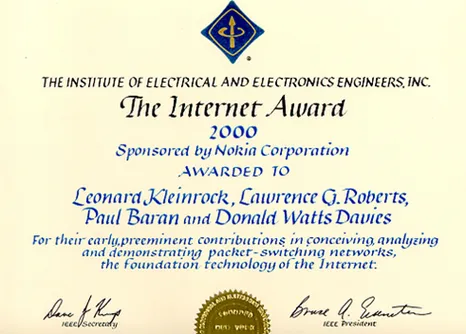
\includegraphics[width=0.6\textwidth]{../assets/ch01/ch01-1_0_通信网络简史-037.png}
\caption{Rober Kahn}
\end{figure}

随着 ARPANET 的发展
\begin{figure}[htbp]
\centering
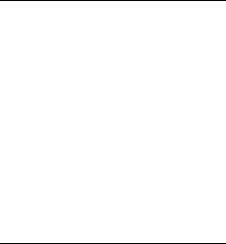
\includegraphics[width=0.8\textwidth]{../assets/ch01/ch01-1_0_通信网络简史-022.png}
\end{figure}和用户对网络需求的不断提高，人们开始发现 NCP 协议存在着很多的缺点，比如 NCP 只能在同构环境中运行（指网络上的所有计算机都运行着相同的操作系统），又比如 NCP 支持的主机数量有限。对于一个分布广泛的网络而言，这些缺陷就必然成为了发展路上最大障碍。
1973 年，针对 NCP 协议存在的问题
\begin{figure}[htbp]
\centering
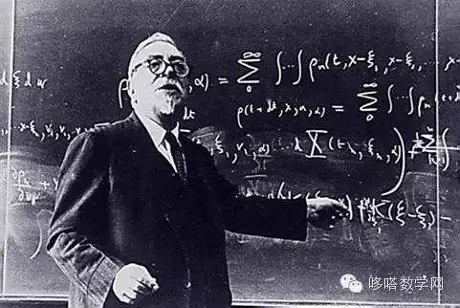
\includegraphics[width=0.8\textwidth]{../assets/ch01/ch01-1_0_通信网络简史-023.png}
\end{figure}，鲍伯·卡恩认识到只有在深入理解了各种操作系统细节的基础上，才能建立一种对各种操作系统都使用的协议。于是鲍伯·卡恩提出了 "开放的网络架构" 思想。同年，来自斯坦福大学的温顿.瑟夫（Vinton G. Cerf）加入 ARPA。鲍伯·卡恩邀请温顿.瑟夫一起研究新协议的各个细节，并在不久就共同提出了 TCP 传输协议。为了验证 TCP 协议的可用性，INWG 开始试验基于 TCP 协议 Client 软件将一个数据发送到距离 10 万公里外的 Server。结果观察数据在传输过程中没有任何丢失，TCP 协议的可行性得到了验证，也一度引起相关领域的广泛关注。1977 年，APRA 改建的 DARPA（美国国防部高级研究计划署）与 BBN 公司、斯坦福大学和伦敦大学学院签订商业合同，正式开始在不同的 CPU 硬件平台上开发 TCP 协议的验证版本：TCPv1 和 TCPv2。随后 1977 年 11 月，鲍伯·卡恩和温顿.瑟夫基于 TCPv2 完成了一个具有里程碑意义的实验。数据包从一辆载有无线传输器的箱式货车发出，进入 APRANET，然后通过专用卫星链路到达伦敦，再通过卫星传输网络，到达 APRANET， 最后传回南加州大学信息科学研究所，行程 9.4 万英里，没有丢失一个比特的数据信息。
1978 年，温顿·瑟夫、鲍伯·卡恩、丹尼·科恩（Danny Cohen）和约翰·普斯特尔（Jon Postel）合力将 TCP 协议从分层思想的角度划分为 2 个协议，即：
  ● 传输层的 TCP 协议，负责可靠传输。
  ● 网络层的 IP 协议，负责在不同的网络之间进行互联。
它们合称 TCP/IPv3
\begin{figure}[htbp]
\centering

\includegraphics[width=0.8\textwidth]{../assets/ch01/ch01-1_0_通信网络简史-024.png}
\end{figure}，并在不久的将来演进为稳定版本 TCP/IPv4。实际上，TCP/IP 协议的发展也并非一帆风顺，其中最大的竞争对手就是国际标准化组织（ISO）。ISO 在制定国际化标准上经验十足，很快就提出了 OSI 七层模型，并大力推广。面对挑战，那时温顿.瑟夫努力劝说让 IBM、DEC、HP 等主机大厂支持 TCP/IP 协议，但都遭到了拒绝。因为在他们看来 TCP/IP 只是一届研究项目，无力与在商业社会中获得过巨大成功的 ISO 抗衡。而美国国防部的应对策略则是将 TCP/IP 协议与 UNIX 系统、C 语言捆绑在一起。1981 年，TCP/IP 协议实现到 UNIX 操作系统（伯克利的研究生Bill Joy实现了BSD Socket）。 TCP/IP 协议与 UNIX 系统、C 语言捆绑在一起，并由 AT&T 向美国各个大学发放非商业许可证。迫使这些跟 UNIX 系统有紧密联系的企业转向 TCP/IP 的怀抱。这为 UNIX 系统、C 语言、TCP/IP 协议的发展拉开了序幕，它们分别在操作系统、编程语言、网络协议这 3 个关键领域影响至今。 到1983年，所有的主机均运行TCP/IP协议。之后网络站点的设计和网络应用的开发促进了Internnet的发展。
后来，美国国家科学基金会（NSF）
\begin{figure}[htbp]
\centering
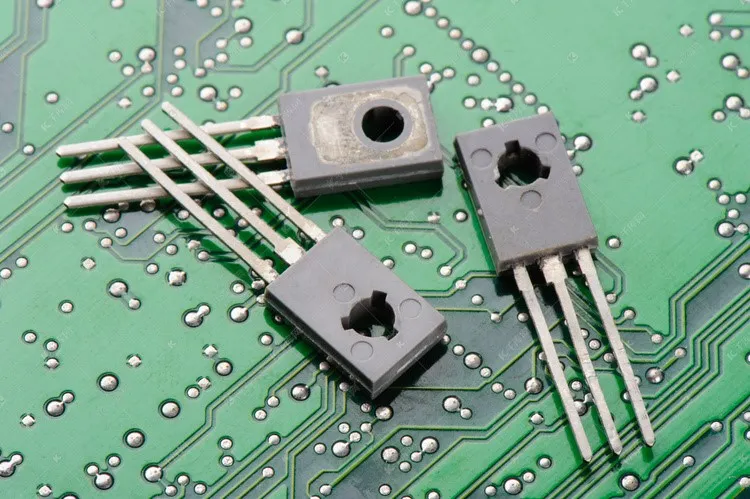
\includegraphics[width=0.8\textwidth]{../assets/ch01/ch01-1_0_通信网络简史-026.png}
\end{figure}自己出资，基于 TCP/IP 协议，建立完全属于自己的NSFnet 广域网。 NSFnet 的发展非常迅速，很快将全美各地的大学、政府和私人科研机构连接起来。同时，NSFnet 的网络速度也很快，比当时民用的 ARPANET 要快 25 倍以上。渐渐地，NSFnet 开始取代 ARPANET，成为 Internet 的主干网。80 年代末，连接到 NSFnet 的计算机数量远远超过了 ARPANET 用户的数量。直至 1990 年 6 月 1 日，ARPANET 正式退出历史舞台。1991年NSF计划由ISP来接管Internet service。ISP可以部署管理自己的骨干网了。各个局域网可以接入ISP，同时ISP之间互联互通。商业的在线服务可以提供Internet连接。计算机工业也进入Internet市场。

\begin{figure}[htbp]
\centering
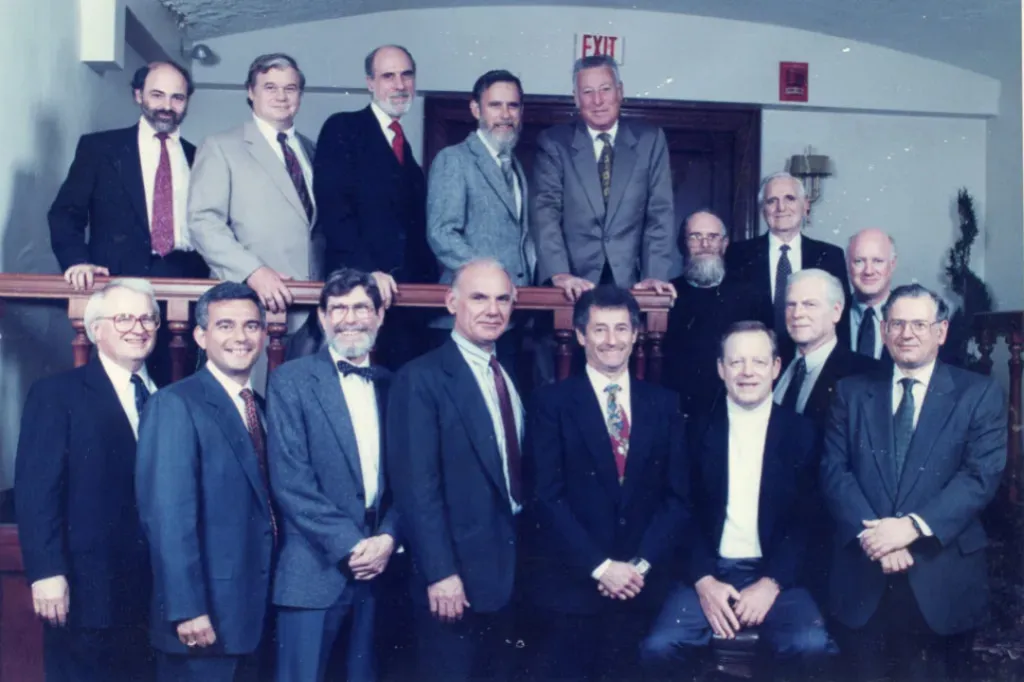
\includegraphics[width=0.9\textwidth]{../assets/ch01/ch01-1_0_通信网络简史-038.png}
\caption{2000年IEEE Internet Award获奖者合影}
\end{figure}

2000年， IEEE Internet Award颁发给
\begin{figure}[htbp]
\centering
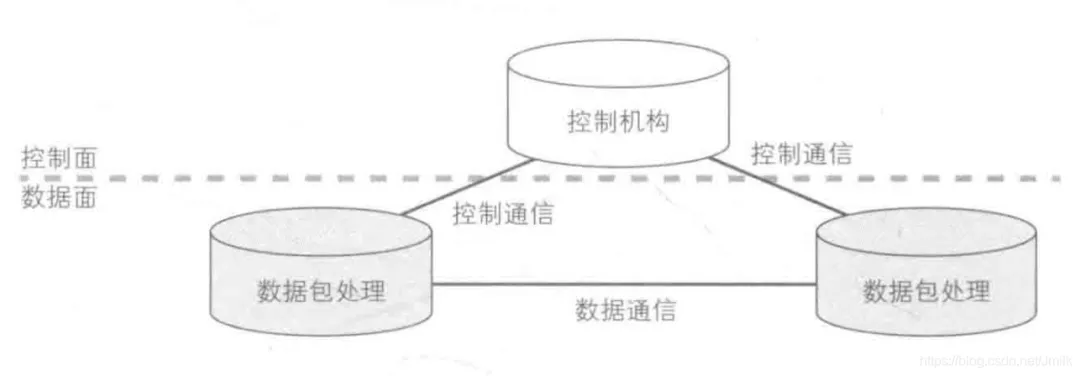
\includegraphics[width=0.8\textwidth]{../assets/ch01/ch01-1_0_通信网络简史-044.png}
\end{figure}雷纳德•克兰罗克（Leonard Kleinrock）、拉里•罗伯茨（Lawrence G. Roberts）、文特•塞尔夫 (Vinton Cerf) 和 罗伯特•卡恩 (Robert Kahn) "for their early, preeminent contributions in conveiving, analyzing and demonstrating packet-switching networks, the fundation technology of the Internet". 1994 年，举办互联网大会 前排从左到右：Dave Walden, Barry Wessler, Truett Thach, Larry Roberts, Len Kleinrock, Bob Taylor, Roland Bryan, Bob Kahn. 后排从左到右：Marty Thrope, Ben Barker, Vint Cerf, Severo Ornstein, Frank Heart, Jon Postel, Doug Englebart, and Steve Crocker.
电话网模拟话音通道的数据通信
\begin{figure}[htbp]
\centering
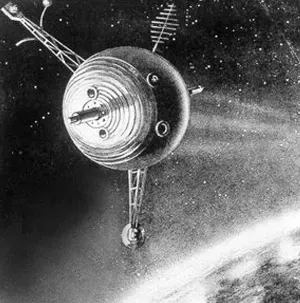
\includegraphics[width=0.8\textwidth]{../assets/ch01/ch01-1_0_通信网络简史-028.png}
\end{figure}。数据网络的一个主要技术难点是要使用普通的电话话音信道访问数字骨干网以及主机计算机。因为在音频信道传输失真，在超过2400b/s的数据传输时会导致错误。为了解决这个问题，1965年贝尔实验室的Robert W. Lucky开发了自适应的modem补偿相位和幅度的失真。自适应设备使得数据速率达到9600b/s，以及低的数据率。尽管做了很多革新性的产品，AT&T并不像其他公司积极销售新的先进modem产品。例如，Codex Corp 才是9600b/s的modem的领导者。同期，还产生了很多先进的技术，例如QAM，OFDM保证了更高的数据率，成为21世纪专线接入、无线广播通信的关键技术。卷积码通过冗余来避免传输错误的影响，Andrew Viterbi在1967年发明的解码算法也是编解码技术的进步。1972年到1980年的8年间，国际电信界集中研究电信设备数字化。统一了话音信号数字编码标准，数字传输系统代替模拟传输系统（数字复用器代替载波机，数字电子交换机代替模拟机电交换机，发明了分组交换机）。
光纤通信。1960s中后期
\begin{figure}[htbp]
\centering
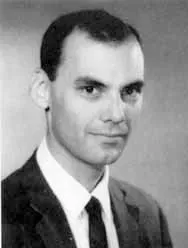
\includegraphics[width=0.8\textwidth]{../assets/ch01/ch01-1_0_通信网络简史-030.png}
\end{figure}的一项有深远影响的技术发展是光纤。在1959-1960年研究者发明了激光器，能够产生相干、直线、单色光束。起初，激光仅仅是实验室的研究工具。但是工程技术人员发现激光可以利用光频率的巨大带宽发送大量的信息。然而，这需要开发low-loss，guided，well-controlled光传输媒体。1966年迎来了巨大的突破。高锟和G.A.Hockham在英国Standard Telecommunication Laboratories （STL）得到一个重要的理论发现：透明材质中的杂质才是造成衰减率过大的主要原因。1970年，终于制造出了符合理论的低损耗试验性光纤，由此开启了光通信的时代。高琨选择了放弃"光纤"专利，选择让全球人民免费享受光纤传输的快速和便捷！1970年康宁公司开发了20dB/km的光纤。同年，贝尔实验室演示了在同样的衰减下使用半导体激光器获得成功的传输。1975年到1988年间，光纤通信传输也获得巨大的进展。AT&T在1988年测试海底光缆TAT-8。其他公司，如日本的NTT也在积极发展光纤技术。1983年NTT部署80公里可以支持400Mb/s数据传输。
本地局域网取得了很大的进步
\begin{figure}[htbp]
\centering
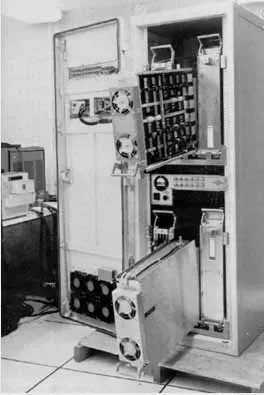
\includegraphics[width=0.8\textwidth]{../assets/ch01/ch01-1_0_通信网络简史-031.png}
\end{figure}。在1972年以太网之父Robert Metcalfe在施乐公司(Xerox Palo Alto)负责设计一种网络将PARC的计算机和ARPANET进行互联。Metcalfe最初将这个网络命名为ALTO ALOHA，直到1973年5月正式运行之后将其改名为"Ethernet"。1979年Metcalfe离开Xerox创办3COM公司，并成功说服DEC、Intel和Xerox一起将Ethernet标准化，并于1980年推出第一版以太网标准（也称为DIX标准），1982年推出了第二版标准Ethernet II（RFC894，也是迄今应用最广泛的标准）。与此同时，IEEE也在1983年推出了802.3标准（RFC1042）。但是由于第一种大规模使用的TCP/IP系统(4.2/3 BSD UNIX)的出现时间介于RFC 894和RFC 1042之间，它为了避免不能和别的主机互操作的风险而采用了RFC 894的实现，所以今天的实际环境中大多数 TCP/IP设备都使用Ethernet II格式的帧。
无线通信技术也开始了全球部署阶段
\begin{figure}[htbp]
\centering
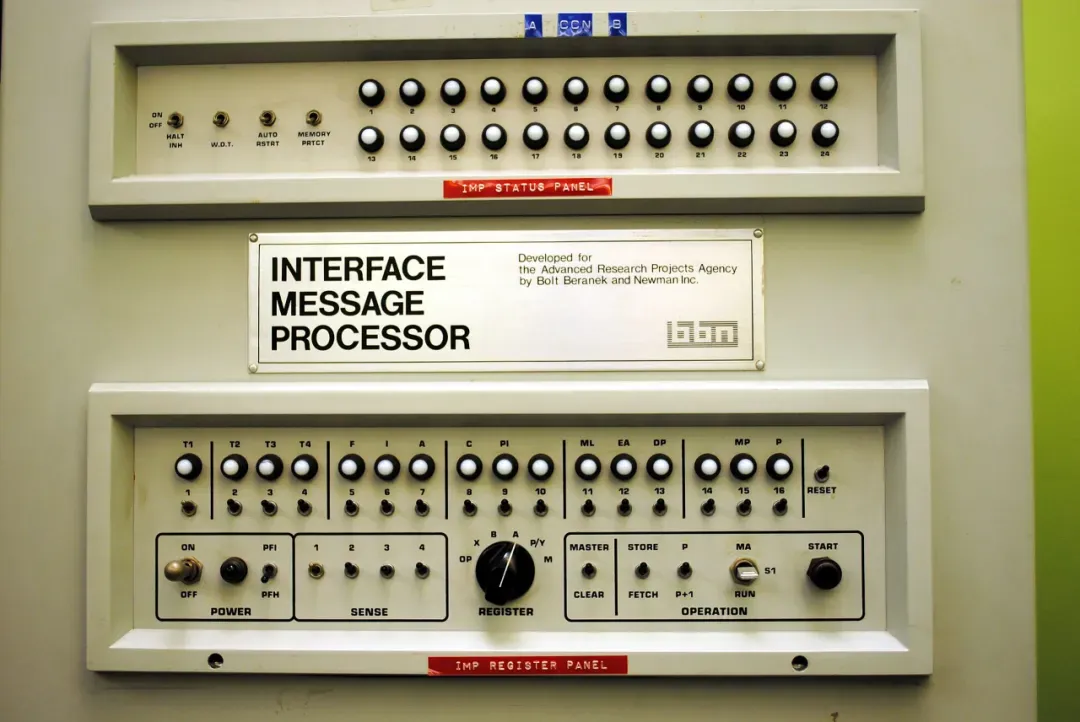
\includegraphics[width=0.8\textwidth]{../assets/ch01/ch01-1_0_通信网络简史-032.png}
\end{figure}。第一个蜂窝网系统 The Advanced Mobile Phone System（AMPS）由贝尔实验室于1978年在北美部署。1984年Jack Winters发表了Multipel in Multiple Out（MIMO）天线系统的论文，通过多个空间路径大幅增加系统性能。1980s中期2G服务和手机业务开始应用，有很多主要的标准如 欧洲TDMA系统GSM、北美TDMA系统IS-136、CDMA系统IS-95。2000年，提出第三代多媒体蜂窝移动通信系统标准，包括欧洲WCDMA，美国的CDMA2000，和中国的TD－SCDMA。2010年，4G发展和2019年5G元年开始。
HTTP 协议与 Web 世界的诞生
\begin{figure}[htbp]
\centering
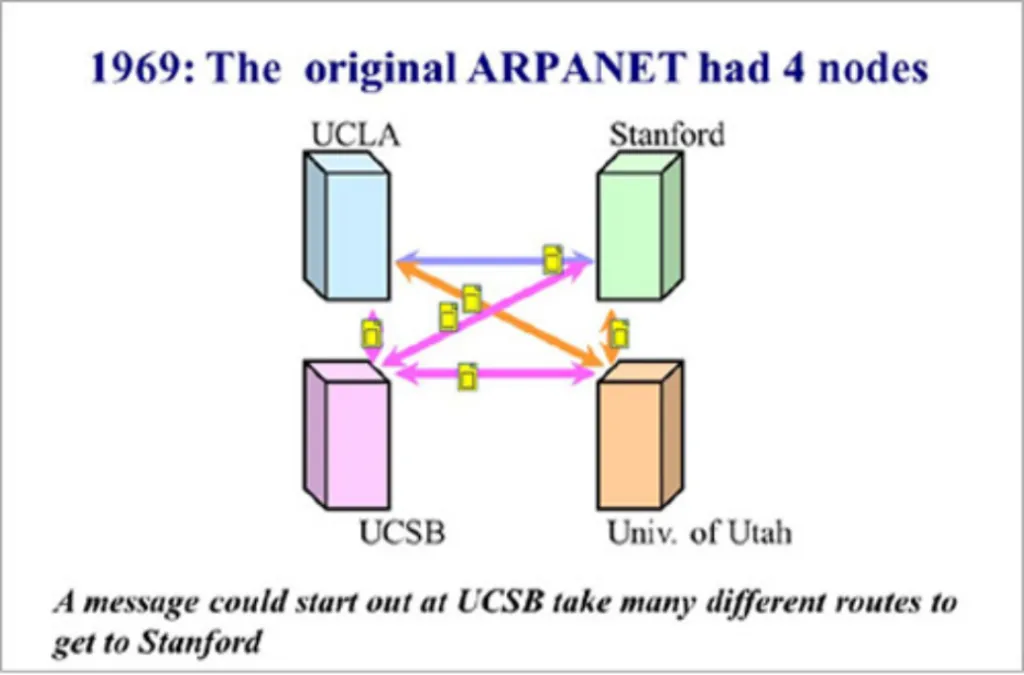
\includegraphics[width=0.8\textwidth]{../assets/ch01/ch01-1_0_通信网络简史-033.png}
\end{figure}。1989 年，当时在瑞士日内瓦 CERN（核子研究中心）工作的Tim Berners-Lee（蒂姆·伯纳斯·李）在论文中提出了一种可以在 Internet 上构建超链接文档的技术，即 HTTP/Web 技术，并提出了 3 点基本要素：
 1. 「URI（Uniform Resource Identifier，统一资源标识符）」：Internel 中的统一资源标识符，用于唯一标识一个 Internet 上的资源。
 2. 「HTML（Hyper Text Markup Language，超文本标记语言）」：使用 HTML 标签来构建超文本文档，HTML 标签将文字，图形、动画、声音、表格、链接等内容格式进行了统一。
 3. 「HTTP（Hyper Text Transfer Protocol，超文本传输协议）」：最初设计来用于传输 HTML的协议，处于 TCP/IP 应用层，传输的数据主体称为 Message（消息），基于 TCP 传输协议。
1990 年 12 月 25 日
\begin{figure}[htbp]
\centering
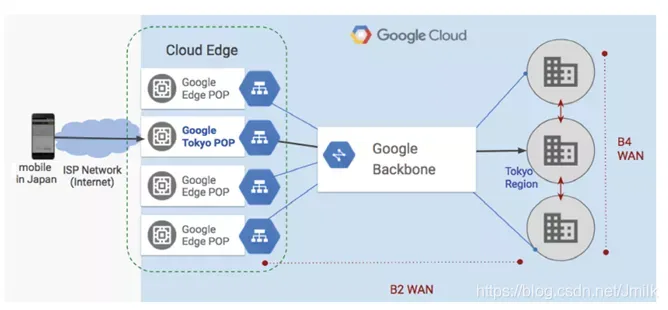
\includegraphics[width=0.8\textwidth]{../assets/ch01/ch01-1_0_通信网络简史-045.png}
\end{figure}，Tim Berners-Lee 和罗伯特·卡里奥一起实现了基于 HTTP 协议的 Web Server，并通过 Internet 成功完成了 HTTP Client 和 Web Server 的第一次通信。1991 年 8 月6 日，Tim Berners-Lee 基于 HTTP 和 HTML 设计并开发了第一个网页浏览器，并发布了世界上第一个 Web 网站。同年，Tim Berners-Lee 正式提出了 WWW（World Wide Web，万维网）的概念。1992 年，几个 Internet 组织合并成立统一的 ISOC（因特网协会）。 1994 年 10 月 1 日，Tim Berners-Lee 创建了非营利性的 W3C（World Wide Web Consortium，万维网联盟）, 由Tim Berners-Lee 担任 W3C 的主席，致力推动 WWW 协议的标准化，并进一步推动 Web 技术的发展。1999 年，HTTP/1.1 发布并成为标准，写入 RFC。至此，HTTP 协议已然成为了 Web世界的奠基石。1992 年，由 HTTP/1.0 和 1.1 的主要设计者 Roy Thomas Fielding 宣布成立了Apache 软件基金会，并作为 Apache 基金会的第一任主席。目前，Apache 软件基金会已成为了全球最大的开源组织之一，孵化了包括：Tomcat、Hadoop 等开源项目。04年TCP/IP, 16年WWW 以及2023年以太网分别获得了图灵奖。

\begin{figure}[htbp]
\centering
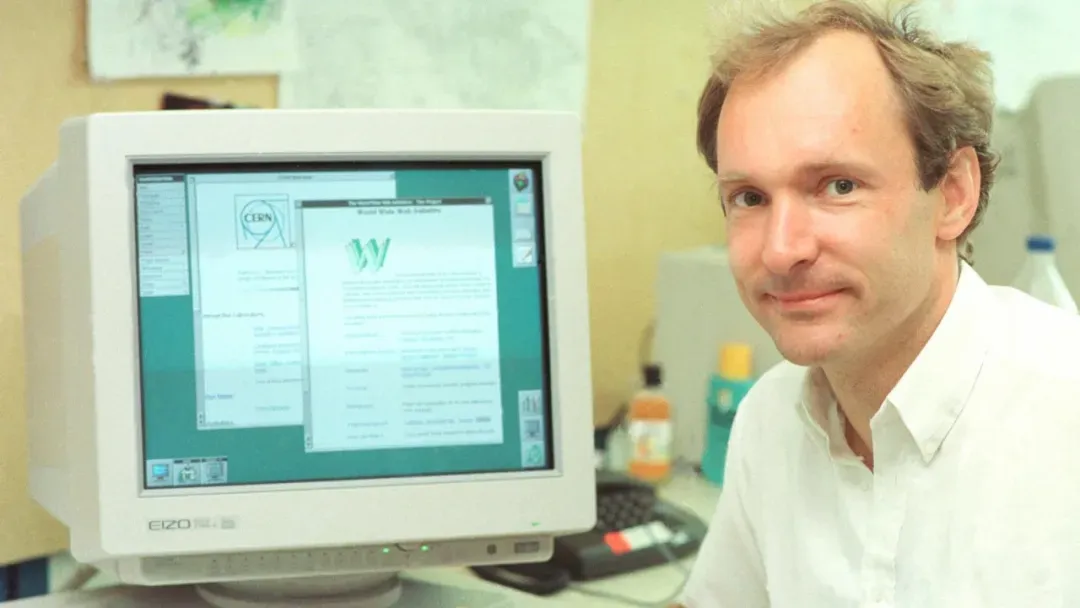
\includegraphics[width=0.9\textwidth]{../assets/ch01/ch01-1_0_通信网络简史-039.png}
\caption{Tim Berners-Lee与万维网}
\end{figure}

云计算的发展
\begin{figure}[htbp]
\centering
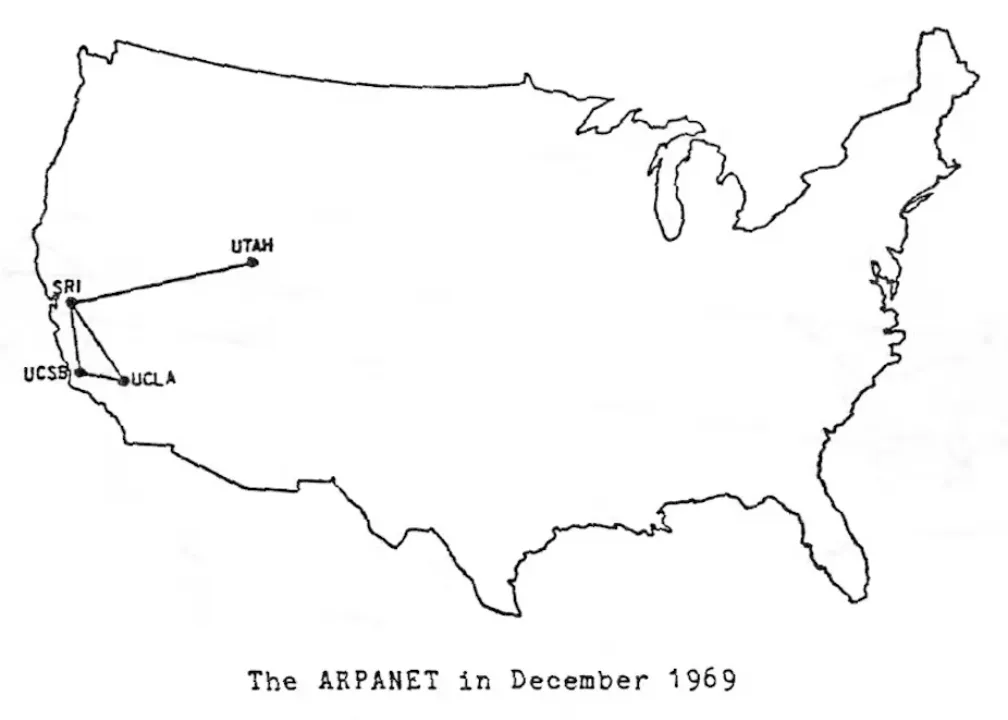
\includegraphics[width=0.8\textwidth]{../assets/ch01/ch01-1_0_通信网络简史-034.png}
\end{figure}。1997年10月，得克萨斯大学的拉姆纳特·切拉帕(Ramnath Chellappa)博士在国际运筹学与管理科学学会年会上，提出计算已经从以大型机为基础的结构进化到了以网络为基础的架构，他把这种新的计算模式称为云计算，这是云计算这个术语在学术界第一次被使用。2006年3月14日，亚马逊 AWS发布了 Amazon Simple Storage Service (Amazon S3)，开始以 Web 服务的形式提供 IT 基础设施服务(laaS 类型)，以较低的价格将空闲IT资源"租"给向企业，开创了一种崭新的计算资源服务模式，它是业界公认最早的云计算服务，这是云计算服务最初的模样。2006年8月9日，谷歌CEO埃里克·施密特(EricSchmit)在加州圣何塞召开的搜索引擎大会上第一次用云和云计算的概念来描述谷歌所提供的互联网服务。埃里克特别指出与此相对应的传统模式就是Oracle主导的传统的客户机/服务器处理结构模式。同年8月25日，亚马逊推出了EC2(弹性云计算)的测试版，EC2是亚马逊云计算服务平台AWS中最重要的部分。2008年，谷歌的云服务开始提供正式服务，AWSEC2有了SLA(服务级别协议)。2009年，阿里云成立，国内云计算市场开始起步。2017年AWS和阿里云均实现了硬件加速的虚拟化架构。
"云计算"逐渐成为互联网服务、应用和存储的核心平台。例如，将数字照片存储在"云端"服务器上远比保存在个人电脑中更高效，因为数据中心的环境更稳定（温度可控、电力供应充足且具备冗余），而家用电脑则容易受到日常使用（如儿童操作、液体泼洒、断电等）的影响。此外，用户通常每隔几年升级一次电脑，需要迁移所有数据，而云端存储则能自动备份和恢复，用户甚至可能察觉不到硬件故障的发生。当今的数据中心已经从松散连接的工作站集群（构成了互联网的雏形）发展成了庞大的"仓库级计算机"，能够运行最复杂的计算任务。硬件构建模块被封装成约40台服务器的"机架"，并通过高性能网络互连多个机架，形成由数百或数千台服务器组成的"集群"。
Future Internet（未来互联网）
\begin{figure}[htbp]
\centering
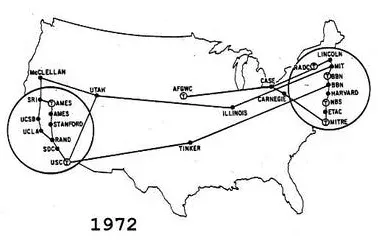
\includegraphics[width=0.8\textwidth]{../assets/ch01/ch01-1_0_通信网络简史-035.png}
\end{figure}的演进成为了业界关注的焦点。并且长期以来，计算机网络领域对 Future Internet 的发展都存在着 2 种不同观点：
 1. 「演进派」：认为 Internet 应像过去那样继续存在，遇到什么样的问题，就打什么样的补丁，安全性此类问题病不是由网络基础架构本身引起的。应该采用网络重叠的方式来提供所需安全性和性能，而不触动现有的基础设施。2008 年 12 月，互联网创建人之一 Bob Kahn 在印度海德拉巴举办的 "互联网治理论坛"上发言，提出了 "数字对象架构" 的新标准，旨在使信息能在互联网上更顺畅地传输。他坚持认为这样就能解决问题，而又不损害基本的架构。
 2. 「革命派」：则认为 Internet 应该被 "重新发明"，不断打补丁的方式，会增加 Internet 的复杂性，使其变得更难以管理、对突破性的新型应用更不友好，且使 Internet 的技术体系逐步僵化，现有体系可能已快走到尽头，还能修补的余地已经不大。2005 年，作为 Internet 协议的总设计师之一的 Dave Clark 教授发表了一篇题为《互联网不再联》的文章，指出："Internet 的本质缺陷让商家花费了几十亿成本，但却阻碍了新发明，威胁到了国家安全。现在到了从头再来的时候了。" 革命派倡导新路线有可能孵化更多种类的网络体系，并创造持续创新的环境。在走革命路线的过程中，也会为演进路线提供更多的改进机会。显然的，演进派的拥趸主要来自商业社会，而革命派则得到了学术界和国家机构的支持。
2005 年 8 月 ， NSF （ 美 国 国 家 科 学 基 金 会 ） 投 资 了 GENI （ Global Environment for Networking Innovations，全球网络创新研究环境）和 FIND（Future Internet Network Design，未来的互联网设计）两个项目。
GENI 项目是一个开放的
\begin{figure}[htbp]
\centering
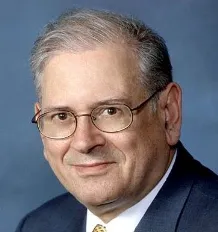
\includegraphics[width=0.8\textwidth]{../assets/ch01/ch01-1_0_通信网络简史-036.png}
\end{figure}、大规模的、真实的、分布式的，用于研究未来互联网技术（Future Internet technologies）的全国性网络创新试验床基础设施。
2007 年 3 月
\begin{figure}[htbp]
\centering
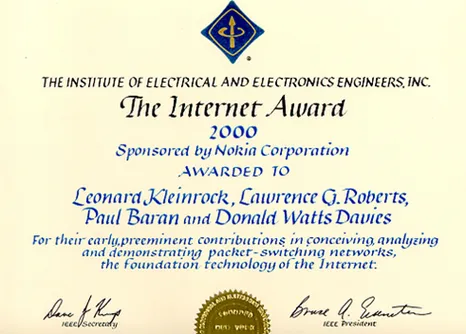
\includegraphics[width=0.8\textwidth]{../assets/ch01/ch01-1_0_通信网络简史-037.png}
\end{figure}，NSF 通过 GENI 和 FIND 项目资助几项大学研究，斯坦福大学的一个跨学科研究项目 Clean Slate Program（意为：白手起家，或从头再来）就是其中之一。Clean Slate 项目的最终目的是要重新发明
\begin{figure}[htbp]
\centering
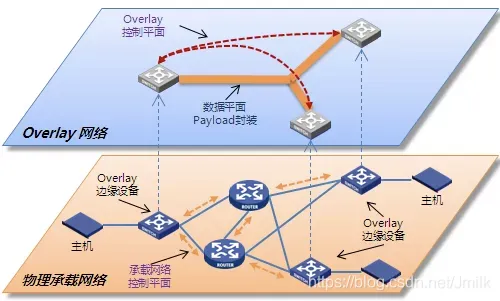
\includegraphics[width=0.8\textwidth]{../assets/ch01/ch01-1_0_通信网络简史-046.png}
\end{figure} Internet，旨在改变设计已略显不合时宜，且难以革命性进化发展的传统网络基础架构。斯坦福教授 Nick McKeown（时任 Clean Slate 项目主任）的博士学生 Martin Casado，试图通过一个集中式的 Controller（控制器），让网络管理员方便地定义基于网络流的安全控制策略，并将这些安全策略应用到各种网络设备中，从而实现对整个网络通讯的安全控制。将传统网络设备的数据转发（Data Plane）和路由控制（Control Plane）两个功能模块相分离，并通过集中式的 Controller （实际采用分布式的 Controller 来取代集中式的 Controller。这样可以管理更大的网络，提供更强劲的性能，还能增强系统的安全性和可靠性。）以标准化的接口对各种网络设备进行管理和配置，那么这将为网络资源的设计、管理和使用提供更多的可能性，从而更容易推动网络的革新与发展。
 ● 「控制面、数据面统一的传统路由器设备」：
 ● 「控制面、数据面分离的 SDN
\begin{figure}[htbp]
\centering
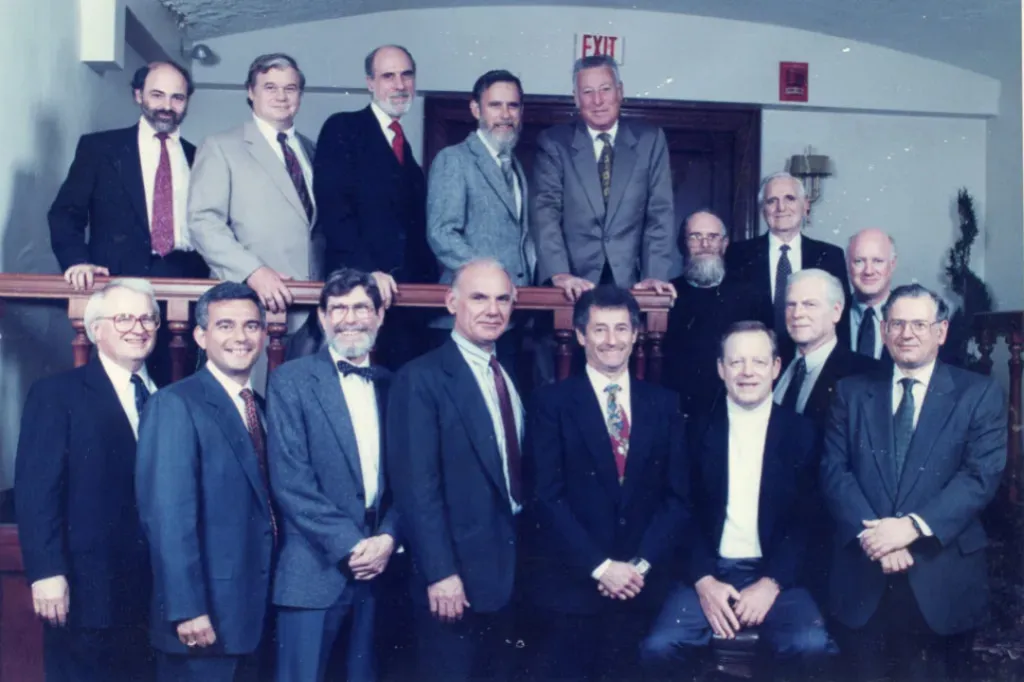
\includegraphics[width=0.8\textwidth]{../assets/ch01/ch01-1_0_通信网络简史-038.png}
\end{figure} 网络架构」：
2011 年，成立了开放网络基金会
\begin{figure}[htbp]
\centering
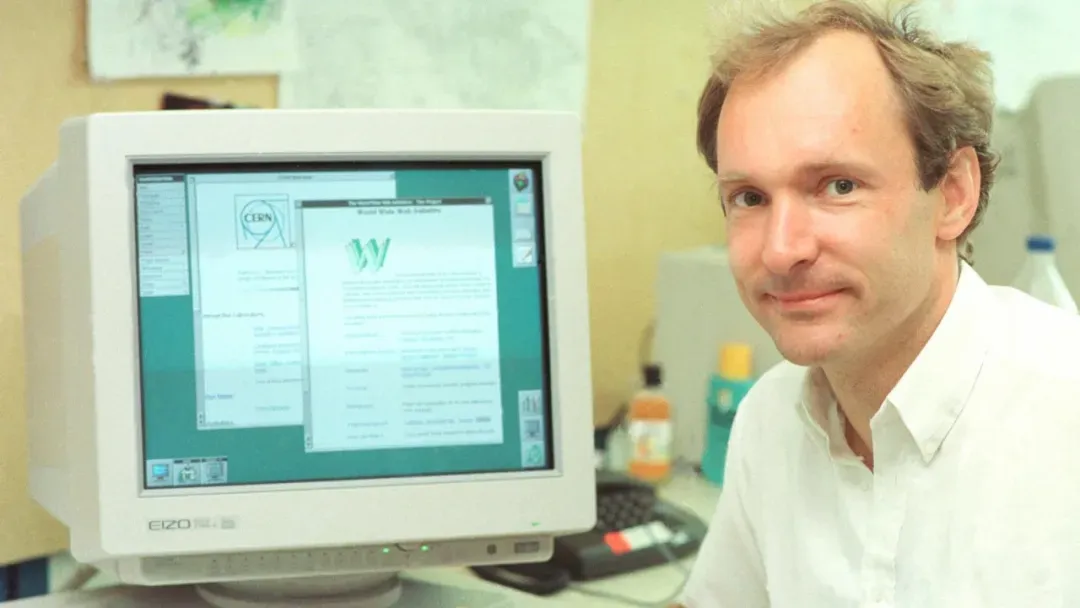
\includegraphics[width=0.8\textwidth]{../assets/ch01/ch01-1_0_通信网络简史-039.png}
\end{figure}（ONF，Open Networking Foundation）。ONF 最初的主要发起成员包括德国电信、Facebook、Google、Yahoo、Microsoft 等公司。这些公司要么是网络服务提供商，要么是电信运营商，唯独没有一家网络设备提供商。ONF 成立的目的，是为了推动SDN 和 OpenFlow 协议的发展，由非网络设备提供商组成的 "软件定义网元" 战线联盟。他们希望以此摆脱网络设备提供商长久以来的枷锁，获得更加灵活且契合自身需求的、更加低耗高效的网络基础设施。同年，ONF 召开了第一届开放网络峰会（Open Networking Summit），并发表了SDN 白皮书《Software Defined Networking：The New Norm forNetworks》，为 OpenFlow和 SDN 在学术界和工业界都做了很好的介绍和推广。2012 年召开的第二届 Open Networking Summit 上，Google 宣布已经在其全球各地的数据中心骨干网络中大规模地使用 OpenFlow。完成 SDN 改造之后，Google B4 网络将全面运行在 OpenFlow 上，并且通过 10G 网络链接分布在全球各地的 12 个数据中心，使广域线路的利用率从 30% 提升到 90% 以上，接近 100%。
网络设备商们也纷纷开始押注
\begin{figure}[htbp]
\centering
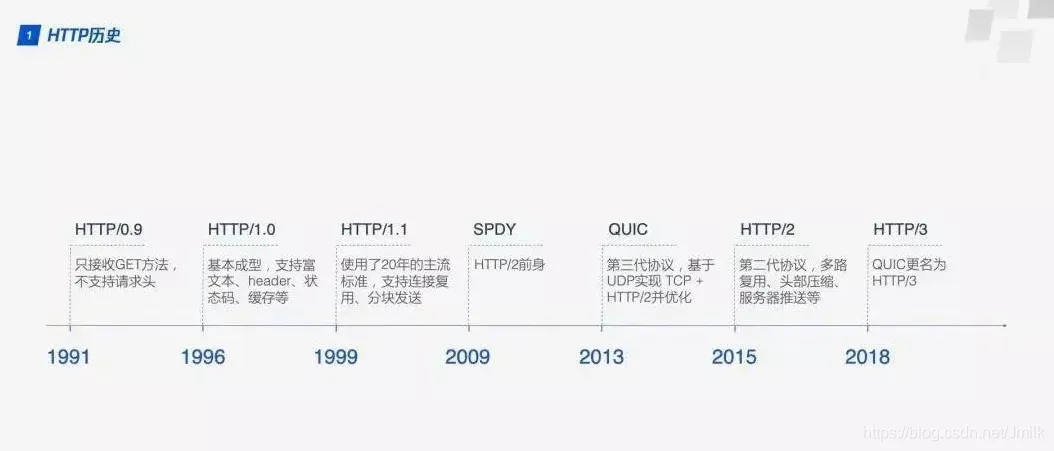
\includegraphics[width=0.8\textwidth]{../assets/ch01/ch01-1_0_通信网络简史-040.png}
\end{figure}走向另外一条更熟悉的道路，即：面向数据中心网络的、基于标准协议（VxLAN、GRE、MPLSoGRE/UDP）的 Overlay 虚拟网络。目前 Overlay 已经大规模被部署到各个云计算数据中心网络中。另一方面，意识到纯软件方向切入网络控制的限制，于是继续从更本质的硬件层面探索 SDN 的可能性，展望未来，网卡、交换机以及协议栈均可编程，整个网络成为一个可编程平台。
未来互联网技术的发展还将继续
\begin{figure}[htbp]
\centering

\includegraphics[width=0.8\textwidth]{../assets/ch01/ch01-1_0_通信网络简史-041.png}
\end{figure}，这场从 21 世纪初开始直至今天的 "革命" 仍未结束。正如计算机体系结构领域的权威、图灵奖得主 David A. Patterson 和 John L. Hennessy 在 2018 年联合发布的论文《A New Golden Age for Computer Architecture》（计算机体系结构的新黄金时代）中所提到的"未来将是计算机体系结构的黄金十年"。同时借助目前人工智能技术的发展，充分促进以网络为切入点的基础设施的进化。

我们的历史故事讲完了
\begin{figure}[htbp]
\centering

\includegraphics[width=0.8\textwidth]{../assets/ch01/ch01-1_0_通信网络简史-042.png}
\end{figure}，这里面还有很多细节可以阅读参考文献。我们可以看到没有哪一份工作是简单完成的，总是在已有的基础上不断改进，不断适应更好的需求来完善。1901意大利工程师马可尼无线电发报机，穿越大西洋的长波无线电信号，获得1909年诺贝尔奖（35岁）。2009高锟因在在光学通信领域光在纤维中传输方面的突破性成就，2018年诺贝尔物理学奖生成高强度超短光脉冲的方法，啁啾脉冲放大（CPA）技术。1956年肖克莱（ Shockley,William Bradford）同巴丁、布拉顿一起因对半导体的研究和发现了晶体管效应，与巴丁和布拉顿分享了1956年度的诺贝尔物理学奖。从这些工作中我们可以看到，诺贝尔物理学奖颁发给在物理前沿研究的，对社会有贡献的的物理学家，而不单单是第一发现人，更是将这一技术推广使其可以应用的水平。历史是螺旋上升的。 未来的发展。做研究遵循两个思路，革新（evoluation），创新（clean state）。用旧的技术解决新问题，用新的技术解决旧问题都是好的，而且也可以落地。更突破性的思维，可以比别人走得更远，同时需要人去推动，给出技术而不去推动，很可能会消失掉。新技术是随着经济的发展，各种自然科学的发展，人们生活方式的改变而不断深入的。当时被看好的技术惨遭淘汰，不被看好的技术却广泛应用，反过来，螺旋上升的社会，可能有一天，在技术水平满足的条件下，那些技术又回到人们的视野中。


\chapter{网络算法学}
% 来源: 19c9fb8c-1472-8ce1-8000-0000e6372a9d_1.2_网络算法学.pdf
% 提取时间: 2026-02-28T22:51:20+08:00

网络算法学
1.2 技术：网络算法学
在本书中，我们将讨论许多具体技术：中断、拷贝和时间轮；Pathfinder和Sting；为什么有些路由器非
常慢；Web服务器是否可以扩展。但是，贯穿本书并使它不仅仅是一本食谱的是网络算法学的概念。如
前所述，网络算法学认识到采用系统方法简化网络实现的重要性。
虽然每个人都知道互联网是由路由器和链路组成的系统，但可能不太明显的是，从Cisco GSR到Apache
Web服务器的每个网络设备也是一个系统。系统由在不同时间点实例化的互连子系统构成。例如，核心
路由器由带有转发引擎和数据包存储器的线路卡组成，这些线路卡通过交叉开关连接。路由器的行为受
到各个时间尺度决策的影响，这些时间尺度从制造时间（当默认参数存储在NVRAM中时）到路由计算时
间（当路由器协同计算路由时）再到数据包转发时间（当数据包被发送到相邻路由器时）。
因此，系统方法中的一个关键观察是，通常可以通过将某些功能在空间上（即移动到其他子系统）或时
间上（即在功能显然需要之前或之后的时间点）移动来设计高效的子系统。从某种意义上说，网络算法
学的实践者是一个不择手段的机会主义者，愿意随时改变规则以使游戏变得更容易。唯一的限制是整个
系统提供的功能继续满足用户的需求。
在马克·吐温的一本书中，一个康涅狄格州的美国佬被传送回亚瑟王的宫廷。然后，这位美国佬用枪与习
惯于用长矛决斗的骑士作战。这是改变系统假设（用枪代替长矛）来解决问题（赢得决斗）的一个例
子。
考虑到网络实现者在高速下所面临的限制——日益复杂的任务、支持更大的系统、少量高速内存和少量
的内存访问——可能需要动用武器库中的每一个技巧、每一把枪来跟上互联网不断增长的速度和规模。
设计者可以投入硬件、改变系统假设、设计新算法——无论采取什么措施都要完成任务。
本书分为四个部分。第一部分是本书的第一章，为将网络算法学应用于数据包处理奠定了基础。第一部
分的第二章概述了模型，第三章介绍了本书其余部分使用的一般原则。




\begin{figure}[htbp]
\centering
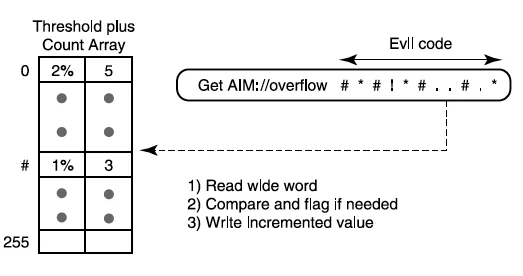
\includegraphics[width=0.8\textwidth]{../assets/ch01/ch01-1_2_网络算法学-003.png}
\end{figure}
图1.3 通过注意到非打印字符的频率来察觉恶意数据包。
快速了解网络算法学的一个好方法是立即进入一个热身示例。虽然下面的热身示例是在可以设计新硬件
的网络设备上下文中，但请注意，第二部分是关于仅使用软件设计技术构建高效服务器的。

                                                    1
1.2.1 热身示例：察觉恶意数据包
想象一下，在企业网络边缘的前端网络监视器（或入侵检测系统）希望标记可疑的传入数据包——可能
包含对内部计算机攻击的数据包。一种常见的此类攻击是缓冲区溢出攻击，攻击者在网络头部字段F中放
置机器代码C。
如果接收计算机为头部字段F分配的缓冲区太小，并且在检查溢出时疏忽大意，代码C可能会溢出到接收
机器的堆栈上。经过更多努力，入侵者可以让接收机器实际执行恶意代码C。然后C接管接收机器。图1.3
展示了这种攻击在一个熟悉的领域中的体现，即目标Web URL（统一资源定位符）。监视器如何检测到
这种可疑URL的存在呢？一种可能的方法是观察到包含恶意代码的URL通常过长（一个简单的检查），
并且通常包含大量不寻常（至少在URL中）的字符，如#。因此，监视器可以将这些数据包（包含过长且
包含过多此类不寻常字符的URL的数据包）标记出来进行更彻底的检查。
值得在一开始就说明，这种策略的安全影响需要仔细考虑。例如，可能有一些无害的程序，如CGI脚本，
在URL中导致误报。在不深入探讨整体架构影响的情况下，让我们假设这是安全架构师交给芯片架构师
的一个规范。我们现在使用这个由Mike Fisk提出的示例问题来说明算法学的实际应用。
面对这样的规范，芯片设计师可能会使用以下设计过程，该过程说明了一些网络算法学的原则。该过程
从一个初步设计方案开始，并使用更好的算法、放宽规范和利用硬件等技术对设计进行改进。
1.2.2 初步方案
检查整体长度很容易实现，因此我们专注于检查可疑字符的普遍性。第一个初步方案如\begin{figure}[htbp]
\centering
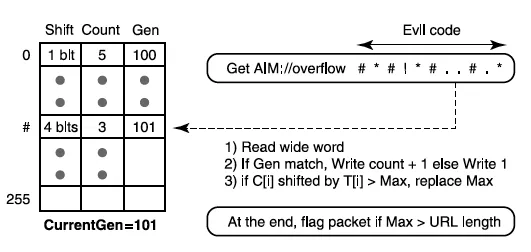
\includegraphics[width=0.8\textwidth]{../assets/ch01/ch01-1_2_网络算法学-004.png}
\end{figure}
图1.4所示。芯片
维护两个数组T和C，每个数组有256个元素，对应8位字符的每个可能值。阈值数组T包含每个字符的可
接受百分比（作为整个URL长度的一部分）。如果URL中某个字符的出现次数超过这个百分比，就应该
标记该数据包。每个字符可以有不同的阈值。
计数数组C中间部分，包含每个可能字符i的当前计数C[i]。当芯片读取URL中的新字符“i”时，它将C[i]增
加1。对于所有i的值，C[i]在遇到新数据包时初始化为0。计数过程在芯片解析HTTP头部并识别URL开始
                                                     2
后启动。
在HTTP中，URL的结束由两个换行符表示；因此，只有在解析完整个URL字符串后才能知道URL的长
度。因此，在URL结束后，芯片对数组C进行最终遍历。如果对于任何j，C[j]≥L·T[j]，其中L是URL的长
度，则标记该数据包。
假设数据包以高速进入监视器，并且我们希望在下一个数据包到达之前完成对一个数据包的处理。这种
要求称为线速处理，在网络中非常常见；它即使在最坏情况下也能防止处理积压。为了满足线速要求，
理想情况下芯片应该对每个URL字节执行少量恒定数量的操作。假设递增计数器的主要步骤可以在接收
一个字节的时间完成。
不幸的是，首先遍历数组初始化它，然后遍历数组检查阈值违规，这使得这个设计速度变慢。最小数据
包大小通常只有40个字节，并且只包含网络头部。再加上768次更多操作（对C的每个元素进行1次写入
和1次读取，并对256个索引中的每一个读取T），这可能使得这个设计不可行。
1.2.3 算法思维
直观上，第二遍遍历数组C和T似乎是浪费。例如，如果任何字符超过阈值就足够报警了。那么为什么要
检查所有字符呢？这表明只需要跟踪到目前为止遇到的最大字符计数c；也许算法只需要检查c是否相对
于总URL长度L超过阈值。




\begin{figure}[htbp]
\centering
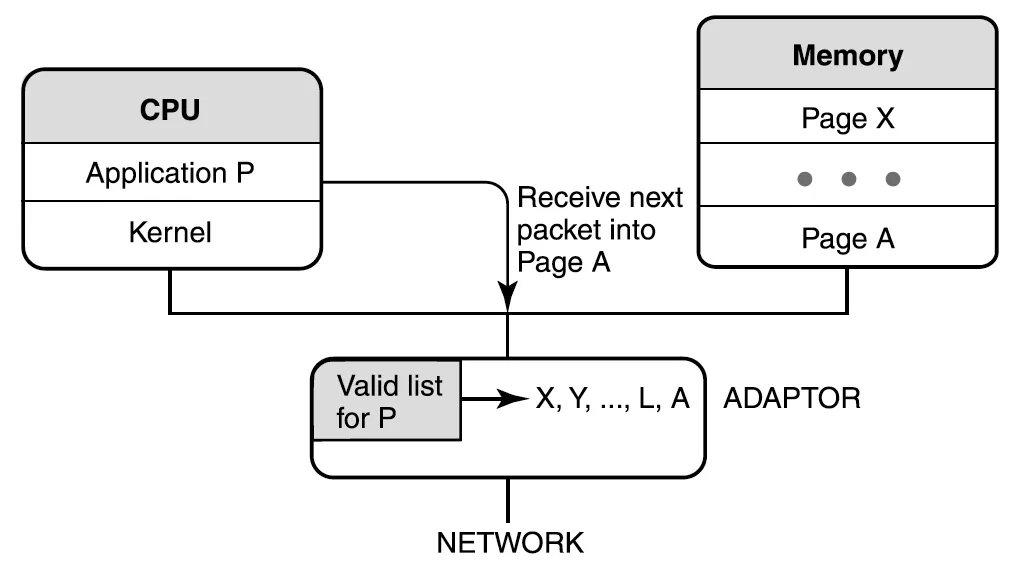
\includegraphics[width=0.8\textwidth]{../assets/ch01/ch01-1_2_网络算法学-005.png}
\end{figure}
图1.5
通过跟踪最高相对计数值Max来避免最后循环遍历阈值数组，该值对应于迄今为止遇到的某个字符k，使
得C[k]/T[k]=Max是所有遇到字符中最高的。如果读取到一个新字符i，芯片增加C[i]。如果
C[i]/T[i]>Max，则芯片用C[i]/T[i]替换当前存储的Max值。在URL处理结束时，如果Max≥L，芯片发出
警报。
这是为什么有效的。如果Max=C[k]/T[k]≥L，显然必须标记该数据包，因为字符k超过阈值。另一方面，
如果C[k]/T[k]<L，那么对于任何字符i，都有C[i]/T[i]≤C[k]/T[k]<L。因此，如果Max低于阈值，则没有
字符超过阈值。因此不可能出现漏报。这个解决方案如图1.5所示。
                                                               3
1.2.4 改进算法：利用硬件
新算法消除了最后的循环，但仍然需要在处理每个字节时进行除法运算。除法逻辑相当复杂，如果可能
的话应该避免——但如何避免呢？
回到规范及其预期用途，看起来阈值不太可能是精确的浮点数。提供阈值的架构师不太可能精确估计这
些值；将2.78%近似为3%而不显著影响安全目标是可能的。那么为什么不进一步将阈值近似为小于精确
目标阈值的2的幂次方呢？因此，如果阈值是1/29，为什么不将其近似为1/32？
以这种方式改变规范需要与系统架构师协商。假设架构师同意这个新提议。那么阈值如1/32可以紧凑地
编码为相应的2的幂次方——即5。这个阈值移位值可以存储在阈值数组中，而不是分数。
因此，当遇到字符j时，芯片像往常一样增加C[j]，然后根据指定的阈值将C[j]左移——除以1/x等同于乘
以x。如果移位后的值高于Max的最后存储值，则芯片用新值替换旧值并继续处理。
因此，处理一个字节所需的逻辑是一个简单的移位和比较。存储状态只是一个寄存器来存储Max。目
前，该设计需要读取阈值数组（读取移位值）、读取计数数组（读取旧计数值）和写入计数数组（写回
增加后的值）。
现在，内存访问——即使是对于最快的片上内存也需要1-2纳秒，对于较慢的内存可能需要长达10纳秒
——比逻辑慢。单个门延迟只有皮秒级，移位逻辑不需要太多门延迟。因此，处理瓶颈在于内存访问次
数。
芯片实现可以通过将两次内存读取合并为一次来优化，如\begin{figure}[htbp]
\centering
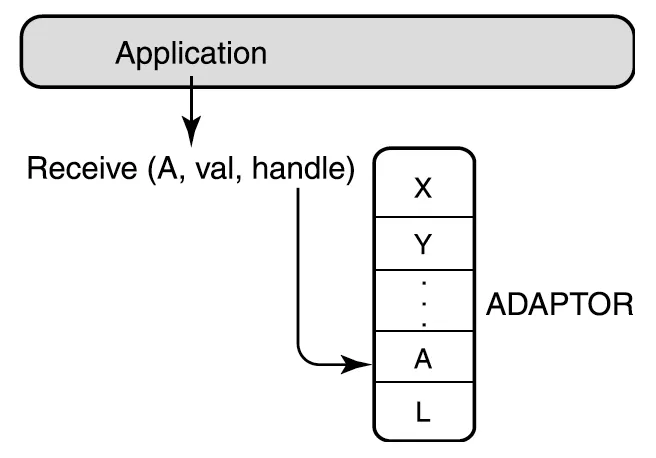
\includegraphics[width=0.8\textwidth]{../assets/ch01/ch01-1_2_网络算法学-006.png}
\end{figure}
图1.6所示。思路是将计数数组和阈值数组合并
为一个更宽的数组。具体来说，使内存字足够宽以容纳计数器（例如，15位来处理长度为32K的数据
包）和阈值（根据所需精度，最多14位）。这样两个字段可以轻松合并成一个更大的字，大小为29位。
实际上，硬件可以处理远大于此的字长，高达1000位。此外，请注意，在软件中提取打包在单个字中的
两个字段相当繁琐，而在硬件中通过适当路由寄存器之间的连线或使用多路复用器则轻而易举。




图1.6

                                                   4
通过合并计数和阈值数组，将两次读取合并为一次，利用宽字和合并数组。
1.2.5 清理工作
我们一直推迟讨论一个棘手的问题。终端循环已经消除，但初始初始化循环仍然存在。要处理这个问
题，请注意芯片在解析完当前数据包的URL后、遇到下一个数据包的URL前有空闲时间。
不幸的是，即使有HTTP头部，数据包也可能小至50字节。因此，即使假设除了URL的10个字节外还有
40个非URL字节的空闲时间，这仍然不足以在无需每字节额外支付6次操作的情况下初始化一个256字节
的数组——每次URL处理过程中每个数组元素需要一次读取和一次写入。
像懒人一样，一种策略是将工作推迟到绝对必要时再进行，希望它可能永远不需要。请注意，严格来
说，芯片不需要在当前数据包中第一次访问字符i之前初始化C[i]。但是芯片如何知道它是第一次看到字
符i呢？
为了实现惰性求值，每个表示合并数组中条目的内存字必须扩展，比如增加一个3位代号G[i]。代号可以
看作是以数据包为单位测量的时钟时间，但它限制为3位。因此，除了每个i的额外G[i]外，芯片还维护另
一个寄存器g，也是3位长；g每处理一个数据包就递增模8。此外，每次更新C[i]时，芯片也会更新G[i]以
反映当前的g值。
有了代号，芯片就不需要在当前数据包处理完后初始化计数数组了。然而，考虑一个代号为h的数据包，
其中包含URL中的字符i。当芯片在处理该数据包时遇到i时，芯片从计数数组中读取C[i]和G[i]。如果
G[i]≠h，这清楚地表明条目i上次被较早的数据包访问过且之后未初始化。因此，逻辑会将C[i]的值写回
为1（初始化加递增）并将G[i]设置为h。如\begin{figure}[htbp]
\centering
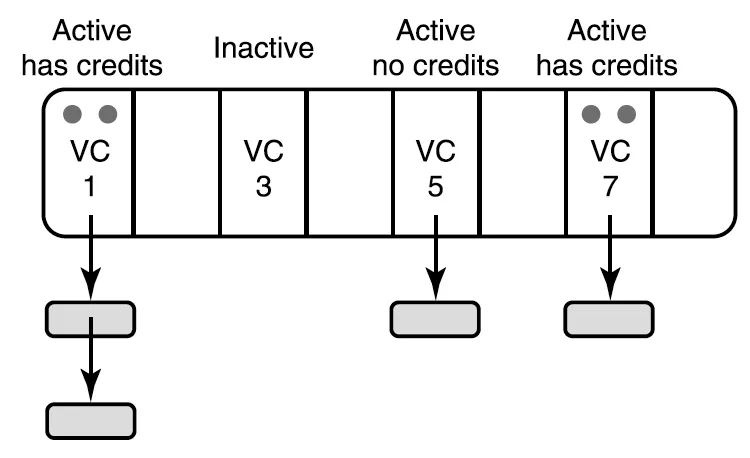
\includegraphics[width=0.8\textwidth]{../assets/ch01/ch01-1_2_网络算法学-007.png}
\end{figure}
图1.7所示。




图1.7
最终解决方案通过代号巧妙地处理初始化循环。
细心的读者会立即提出异议。由于代号只有3位，一旦g的值回绕，就会出现别名问题。因此，如果G[i]为
5且条目i直到八个数据包后才被访问，g将回绕到5。如果下一个数据包包含i，C[i]将不会被初始化，计

                                                   5
数将（错误地）累积当前数据包中的i的计数以及八数据包之前的计数。
芯片可以通过执行一个单独的"清理"循环来解决这种别名问题，该循环读取数组并将所有带有过期代号的
计数器初始化为0。为了正确性，芯片必须保证每处理八个数据包就对数组进行一次完整扫描。假设每个
数据包有（比如说）40个非URL字节空闲时间，这保证了在处理八个数据包后有320个非URL字节的空
闲时间，足以使用每次读取和写入一个字节的方式初始化一个256元素数组，无论该字节是URL字节还是
非URL字节。显然，如果需要更多空闲时间，设计者可以通过增加代号的位数来获得更多空闲时间，代
价是数组中稍微增加的存储空间。
因此，芯片必须有两种状态：一种用于处理URL字节，另一种用于处理非URL字节。当URL完全处理完
后，芯片切换到"清理"状态。芯片维护另一个寄存器，指向要清理的下一个数组条目s。在清理状态下，
当接收到非URL字符时，芯片读取合并数组中的条目s。如果G[s]≠g，则将G[s]重置为g并将C[s]初始化
为0。
因此，使用每个数组条目额外的3位代号减少了初始化处理周期，通过用存储换取处理。总的来说，现在
一个合并数组条目只有32位，15位用于计数器，14位用于阈值移位值，3位用于代号。请注意，在URL字
节处理期间所需的额外初始化检查并没有增加内存引用（瓶颈），但略微增加了处理逻辑。此外，它需
要两个额外的芯片寄存器来保存g和s，这是一笔很小的额外开销。
1.2.6 网络算法学的特点
检测恶意数据包的示例说明了网络算法学的三个重要方面：
a. 网络算法学是跨学科的：鉴于网络处理必须以高速完成，路由器设计者很难不使用硬件。该示例利用
了硬件的几个特性：它假设可以轻松实现任意大小的宽字；它假设移位比除法更容易；它假设内存引用
是瓶颈；它假设片上快速内存中包含256元素数组是可行的；它假设增加几个额外寄存器是可行的；最后
它假设对逻辑进行小改动以结合URL处理和初始化是微不足道的。
对于不熟悉硬件设计的读者来说，这有点像不懂数牌规则就加入一场纸牌游戏，然后发现自己以意想不
到的方式被出牌和压制。本书的一个论点是，掌握一些相关硬件设计知识可以帮助即使是软件设计师也
至少理解不同硬件设计的可行性。本书的另一个论点是，这种跨学科思维有助于产生最佳设计。
因此，第2章介绍了游戏规则。它介绍了硬件、操作系统和网络的简单模型，指出了解决棘手实现问题的
机会。它还介绍了操作系统和网络的简单模型。之所以这样做，是因为像客户端和Web服务器这样的终
端系统需要调整和理解操作系统问题以提高性能，就像路由器和网络设备需要调整硬件一样。
b. 网络算法学认识到系统思维的首要性：规范被放宽以允许近似阈值为2的幂次方，这简化了硬件。放宽
规范和将工作从一个子系统转移到另一个子系统是一种极其常见的系统技术，但这并不是当前大学教育
实践中鼓励的做法，在大学教育中，每个领域都是孤立教授的。
因此，今天有独立的算法课程、操作系统课程和网络课程。这往往鼓励"黑箱"思维，而不是整体或系统思
维。该示例还提到了其他系统技术，如使用惰性求值和用存储换取处理来清理计数数组。
                                                     6
因此，本书的一个特点是试图将算法学中使用的系统原则提炼为15条原则，这些原则列在书的前封面
上，并在第3章中详细探讨。本书试图用这些原则来解释和剖析本书中描述的所有网络实现。这些原则也
标有编号以便于参考，尽管在大多数情况下，我们会同时使用编号和名称。例如，快速浏览前封面你会
发现放宽规范是原则P3，惰性求值是P2b。
c. 网络算法学可以从算法思维中受益：虽然本书强调系统思维的首要性以尽可能巧妙地解决问题，但在
许多情况下系统约束阻止了问题的完全消除。在我们的示例中，在尝试通过放宽规范来巧妙解决问题
后，误报问题导致考虑跟踪相对于其阈值最高的计数器。作为第二个例子，第11章表明，尽管尝试使用所
谓的标签交换来巧妙解决互联网查找问题，许多路由器仍然采用高效算法进行查找。
然而，值得强调的是，由于模型与标准理论模型有所不同，仅仅盲目重用现有算法往往是不够的。例
如，第13章讨论了需要在8纳秒内调度交叉开关的需求，这导致考虑更简单的最大匹配启发式算法，而不
是产生二分图中最优匹配的更复杂算法。
作为第二个例子，第11章描述了BSD实现如何盲目重用一种称为Patricia trie的数据结构来进行IP查找，
该数据结构使用跳过计数，导致算法需要复杂的回溯。一种简单的修改保留了实际跳过的位（而不是计
数），避免了回溯的需要。但这需要对黑盒（即算法）及其应用有一定的洞察力。
总之，不加批判地使用标准算法可能会因为不恰当的度量（例如，对于像BPF这样的数据包过滤器，插
入新分类器可能比搜索需要更多时间）、不恰当的模型（例如，忽略软件中的缓存行或硬件中的并行性
的影响）和不恰当的分析（例如，隐藏了确保线速转发的关键常数因子的大O复杂度结果）而错过实现突
破。
因此，本书的另一个目的是说服实现者，掌握算法洞察力和使用基本算法技术（如分治法和随机化）对
于设计高速网络处理任务至关重要。这引出了以下定义：
定义：网络算法学是采用跨学科系统方法，并辅以算法思维，在服务器、路由器和其它网络设备上设计
高速网络处理任务实现的技术。
本书的第一部分致力于更详细地描述网络算法学方法。第1章的前言部分给出了概述。
 重点            动机           示例主题
 模型            理解操作系统、硬件、网 内存技术技巧（交错、混合
               络的简单模型       SRAM/DRAM）
 策略            学习克服瓶颈的系统原则 传递提示、惰性评估、增加状态、利用
                            局部性
 问题            练习将原则应用于简单问 为网络监视器设计查找引擎
               题
\begin{figure}[htbp]
\centering
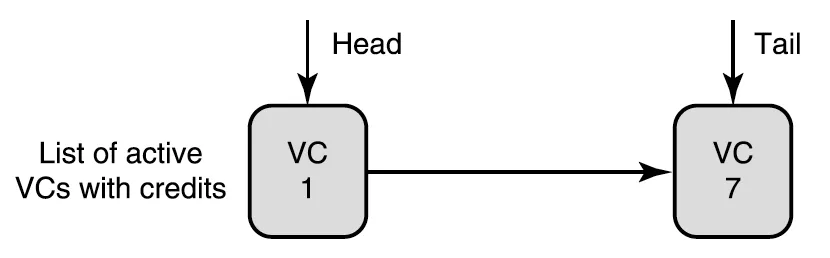
\includegraphics[width=0.8\textwidth]{../assets/ch01/ch01-1_2_网络算法学-008.png}
\end{figure}
图1.8

                                                       7
网络算法学预览。网络算法学通过一组模型、策略和示例问题引入，这些内容在第1章中描述。
虽然本书侧重于网络，但通用算法学方法适用于任何计算机系统的实现，无论是数据库、处理器架构还
是软件应用。第3章通过提供计算机系统实现领域的示例来提及这一更广泛的哲学。只对网络感兴趣的读
者可以放心，除了第3章外，本书其余部分避免了超出网络范围的进一步离题。
虽然第2部分和第3部分为重要特定问题提供了具体技术，但本书的主要目标是使读者能够在软件或硬件
中高速处理任意数据包处理任务。因此，未来的实现者可能会被赋予加速Web服务器中的XML处理（鉴
于当前趋势很可能）甚至在路由器中计算卡方统计量（因为卡方提供了一种检测入侵检测等任务中观察
到的异常频率的测试）的任务。尽管被分配了一个完全陌生的任务，希望实现者能够使用本书描述的模
型、原则和技术来设计这些任务的新解决方案。
十五个实施原则
与其计算，我不得不思考问题，这是一种成功的公式，我强烈推荐。
——伊万·苏泽兰
在理解了国际象棋游戏中皇后和骑士的移动方式之后，了解基本策略（如在残局中将兵升变和王车易
位）是有帮助的。同样，在上一章学习了协议实现游戏的一些规则之后，本章将以15个原则的形式向您
介绍实施策略。这些原则是从运行良好的协议实现中抽象出来的。许多优秀的实现者无意识地使用这些
原则。然而，关键是要阐明这些原则，以便可以有意识地应用它们来制定高效的实现。
本章的结构如下。3.1节通过一个三值内容可寻址存储器（CAM）问题来激励使用这些原则。3.2节使用
网络安全取证问题来澄清算法和算法学之间的区别。3.3节介绍了15个实施原则；3.4节解释了实施原则
和设计原则之间的区别。最后，3.5节描述了在应用这些原则之前应提出的一些警示性问题。
快速参考指南
时间紧迫的读者应查阅\begin{figure}[htbp]
\centering
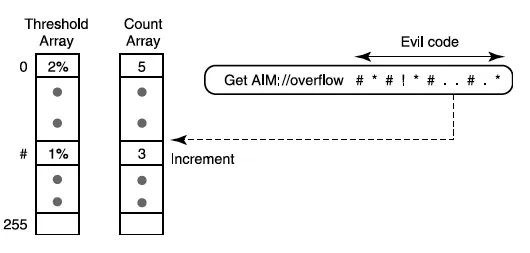
\includegraphics[width=0.8\textwidth]{../assets/ch01/ch01-1_2_网络算法学-001.png}
\end{figure}
图3.1-3.3中总结的15个原则。这些原则的两个网络应用可以在三值CAM更新问题
（第3.1节）和网络安全取证问题（第3.2节）中找到。
3.1 激励使用原则——更新三值内容可寻址存储器
如果一个字符串包含的字符是0、1或*，其中表示可以匹配0和1的通配符，则称该字符串为三值字符串。
长度为3的三值字符串示例包括S1=01和S2=1；实际的二进制字符串011同时匹配S1和S2，而111仅匹配
S2。三值内容可寻址存储器（CAM）是一种包含指定长度的三值字符串及其相关信息的内存；当输入一
个字符串时，CAM会并行搜索其所有内存位置，并在一个周期内输出匹配指定输入键的最低内存位置。
 编号               原则                 应用

                                                     8
P1                避免明显的浪费           零拷贝接口
P2 P2a P2b P2c    在时间上转移计算 预先计算 懒   应用设备通道 写时复制 集成层
                  惰求值 共享费用，批量处理     处理
P3 P3a P3b P3c    放宽系统要求 用时间换取确定    随机公平排队 交换机负载均衡
                  性 用时间换取准确性 在空间上   IPv6分片
                  转移计算
P4 P4a P4b P4c    利用系统组件 利用局部性 用速   基于局部性的接收器处理；
                  度换取内存 利用现有硬件      Lulea IP查找 快速TCP校验和
P5 P5a P5b P5c    添加硬件 使用内存交错和流水    流水线IP查找 共享内存交换机
                  线 使用宽字并行性 有效结合    维护计数器
                  DRAM和SRAM

图3.1
原则1-5的总结——系统思维。
 编号               原则                网络示例
 P6               创建高效的专业化例程        UDP校验和
 P7               避免不必要的通用性         Fbufs
 P8               不要拘泥于参考实现         回调
 P9               在层接口中传递提示         数据包过滤器
 P10              在协议头中传递提示         标签交换

\begin{figure}[htbp]
\centering
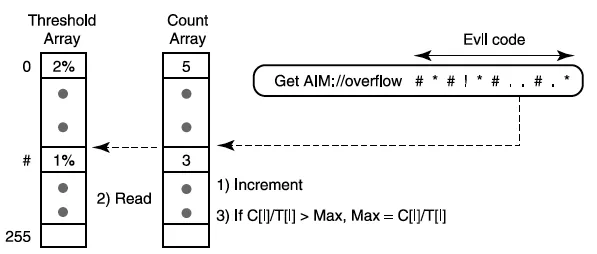
\includegraphics[width=0.8\textwidth]{../assets/ch01/ch01-1_2_网络算法学-002.png}
\end{figure}
图3.2
原则6-10的总结——在保持模块化的同时恢复效率。
图3.4展示了三值CAM在互联网路由器的最长匹配前缀问题中的应用。对于每个传入的数据包，每个互联
网路由器必须从传入的数据包中提取一个32位的目标IP地址，并将其与转发数据库中的IP前缀及其对应
的下一跳进行匹配。IP前缀是一个长度为32的三值字符串，其中所有的通配符都在末尾。我们将稍微改
变符号表示法，让表示任意数量的通配符字符，因此101匹配10100而不仅仅是1010。

                                                          9
编号                原则                网络示例
P11 P11a          优化期望情况 使用缓存       头部预测 Fbufs
P12 P12a          增加状态以提高速度 增量计算    活动VC列表 重新计算CRC
P13               优化自由度             IP前缀树查找
P14               使用桶排序、位图          定时轮
P15               创建高效的数据结构         第4层交换

图3.3
原则11-15的总结——加速关键例程。
图3.4
使用三值CAM进行前缀查找的示例。
因此，在图3.4中，发送到以010001开头的目标地址的数据包匹配前缀010001和01，但应根据互联网转
发的最长匹配规则发送到端口P5。我们将在第11章中详细讨论这个问题。现在，请注意，如果前缀按图
3.4中的方式排列，使得所有较长的前缀都出现在较短前缀之前（如图3.4所示），三值CAM可以在一个
内存周期内提供匹配的下一跳。
虽然三值CAM在消息转发方面非常快速，但它们要求较长的前缀必须出现在较短的前缀之前。然而，路
由协议经常添加或删除前缀。假设在图3.4中，必须向路由器数据库中添加一个新前缀11*，下一跳为端口
1。插入的朴素方法将通过在长度为2的前缀组中创建一个空位（即在0*之前创建一个空位）来实现，方
法是将所有长度为2或更长的前缀向上移动一位。
不幸的是，对于一个典型核心路由器所维护的大约100,000个前缀的大型数据库，这将需要100,000个内
存周期，这将使得添加前缀变得非常缓慢。我们可以通过系统地应用以下两个原则（在本章后面描述为
原则P13和P15）来获得更好的解决方案。
理解和利用自由度
观察图3.4中的转发表，我们看到所有相同长度的前缀都排列在一起，并且所有长度为i的前缀都出现在长
度为j>i的前缀之后。然而，在图中，所有相同长度的前缀也按值排序。因此，00出现在01之前，01出现
在10之前。但对于CAM来说，正确返回最长匹配前缀并不是必需的：我们只需要在不同长度的前缀之间
进行排序；我们不需要对相同长度的前缀进行排序。

                                                     10
观察图3.4的更抽象视图（如图3.5所示），我们看到，如果我们要在长度为i的前缀集合的开头添加一个
条目，我们必须在长度为i+1的前缀集合的末尾创建一个空位。因此，我们必须将已经位于此位置的条目
X移动到另一个位置。如果我们把X向上移动一步，我们将被迫回到之前低效的解决方案。
然而，我们对自由度的观察表明，我们可以将X放置在任何靠近其他长度为i+1前缀的位置。因此，另一
种想法是将X移动到Y的位置，Y是最后一个长度为i+2的前缀。但这又迫使我们为Y找到一个新位置。这
如何帮助我们？我们需要第二个原则。
使用算法技术
递归再次被提出：我们通过将问题简化为同一问题的“更小”实例来解决问题。在这种情况下，为Y分配新
位置的问题的“更小”是因为长度为i+2的前缀集合比长度为i+1的前缀集合更接近CAM顶部的空位。因
此，我们从CAM的顶部开始向下工作，通过在长度为1的前缀集合的末尾创建一个空位，然后在长度为2
的前缀集合的末尾创建一个空位，依此类推，直到我们在长度为i的前缀集合的末尾创建一个空位。因
此，最坏情况下的时间复杂度是32-i次内存访问，对于小的i来说大约是32次。
我们完成了吗？没有，我们可以做得更好，通过进一步利用自由度。首先，在图3.5中，我们假设空位在
CAM的顶部。但空位可以放在任何地方。特别是，它可以放在长度为16前缀之后。这将最坏情况下的内
存访问次数减少了一半（Shah和Gupta，2001）。
一个更复杂的自由度是如下。到目前为止，CAM插入算法的规范要求“如果i>j，则长度为i的前缀必须出
现在长度为j的前缀之前。”这样的规范对于正确性来说是足够的，但并不是必需的。例如，010可以出现
在111001之前，因为没有地址可以同时匹配这两个前缀！
因此，一个不那么严格的要求是“如果两个前缀P和Q可以匹配同一个地址，那么如果P比Q长，则P必须
在CAM中出现在Q之前。”这在Shah和Gupta（2001）中被用来进一步减少某些实际数据库中插入的最
坏情况下的内存访问次数。
虽然最后的改进并不值得其复杂性，但它指向了另一个重要的原则。我们经常将一个大问题分解为子问
题，并将子问题交给基于规范的解决方案。例如，CAM硬件设计者可能已经将更新问题交给微码编写
者，指定较长的前缀必须放在较短的前缀之前。
但是，正如之前所述，这样的规范可能不是解决原始问题的唯一方法。因此，对规范进行更改（原则
P3）可以产生更高效的解决方案。当然，这需要有好奇心和自信的个体，他们能够理解全局，或者有足
够的勇气提出危险的问题。
3.2 算法与算法学
可能会有人争辩说，前面的例子本质上仍然是算法性的，并不需要系统思维。另一个快速的例子将有助
于澄清算法和算法学之间的区别。

                                                   11
安全取证问题
在许多入侵检测系统中，当某个源（例如，通过某些数据包头部定义的源IP地址）被判定为可能行为不
端时，管理员通常会发现该流（例如，发送了100,000个数据包到被攻击子网中的不同机器）的证据通常
已经消失（即，已经被路由器转发）。问题是，概率检查需要在一段时间内累积每个接收到的数据包的
某些状态（例如，在怀疑表中），以便在某个源被判定为可疑之前。因此，如果在10秒后被判定为可
疑，如何回溯并检索该源在这10秒内发送的数据包？
图3.6
保持一个包含过去可疑流发送的最后一个100,000个数据包的队列，其中包含关于可疑流的信息。
为了实现这一点，在图3.6中，我们保持一个由路由器发送的最后一个100,000个数据包的队列。当一个
数据包被转发时，我们还将该数据包的副本（或仅保留指向该数据包的指针）添加到队列的头部。为了
保持队列的有界性，当队列满时，我们从尾部删除数据包。
这种方案的主要困难在于，当一个可疑流被检测到时，队列中可能有很多该流的包（见图3.6）。所有这
些包都必须放入取证日志中以传输给管理员。教科书式的算法方法是为每个流ID添加一些索引结构，以
便快速搜索流ID。例如，可以维护一个流ID的哈希表，将每个流映射到队列中具有该流ID的所有数据包的
指针列表。当一个新的数据包放入队列时，在哈希表中查找流ID，并将新数据包在队列中的地址放在流
的列表末尾。当然，当数据包离开队列时，必须从列表中删除其条目，并且可以保证要删除的条目是该
流ID的第一个条目。
尽管如此，教科书式的方案仍然存在一些困难。它增加了维护每个流ID的额外队列的空间，并且在高速
实现中空间可能非常宝贵。它还增加了数据包处理的额外复杂性，以维护哈希表，并且需要在数据包被
100,000个数据包之后的数据包覆盖之前将流的所有数据包读出到取证日志中。相反，以下“系统”解决方
案可能更为优雅。
解决方案
当F被判定为可疑时，不要试图立即识别所有属于流F的数据包，而是在数据包到达队列末尾时懒惰地识
别它们。如图3.7所示，当我们将一个数据包添加到队列头部时，我们必须从队列尾部删除一个数据包
（至少当队列满时）。
保持一个包含过去可疑流发送的最后一个100,000个数据包的队列，其中包含关于可疑流的信息。
如果该数据包（例如，Q，见图3.6）属于流F，并且流F已达到某种怀疑阈值，我们然后将数据包Q添加
到取证日志中。日志可以发送给管理员。这种方案的额外开销很大，但可以管理；我们必须执行两个数
据包处理步骤，一个用于正在转发的数据包，另一个用于从队列中移除的数据包。但这两种数据包处理


                                                12
步骤在教科书式方案中也是必需的；另一方面，优雅的方案不需要哈希，并且使用的存储空间更少（不
需要在100,000个数据包之间建立指针）。
3.3 十五个实施原则——分类和描述
前面两个例子以及第1章中的热身练习激发了以下15个原则，这些原则将在本书的其余部分中使用。它们
在封面内侧进行了总结。为了增加结构，它们被分类如下：
 ● 系统原则：原则1-5利用了我们正在构建系统的事实。
 ● 在保持模块化的同时提高效率：原则6-10提出了一些方法，可以在允许复杂系统模块化构建的同时
   提高性能。
 ● 加速执行：原则11-15提出了一些技术，用于加速单独考虑的关键例程。

令人惊讶的是，许多这些原则多年来一直被Greasy Spoon餐厅的Chef Charlie所使用。本章有时会使用
来自Chef Charlie的经验示例，以及计算机系统示例。每个原则也描述了一个网络示例，尽管细节将推迟
到后面的章节。
3.3.1 系统原则
前五个原则利用了我们正在构建系统的事实。
P1：在常见情况下避免明显的浪费
在一个系统中，某些操作序列可能存在浪费的资源。如果这些模式经常发生，消除浪费可能是值得的。
这反映了对系统成本的节俭态度。
例如，Chef Charlie需要去食品储藏室拿冰淇淋机来做冰淇淋，去食品储藏室拿馅饼盘来做馅饼。但当他
做冰淇淋馅饼时，他学会了消除两次单独去食品储藏室的明显浪费。
同样，优化编译器会寻找明显的浪费，例如重复的表达式。例如，如果一个语句计算i=5.1n+2，而后续
语句计算j:=(5.1n+2)4，则重复计算公共子表达式5.1n+2是浪费的，可以通过计算子表达式一次，将其赋
值给临时变量t，然后计算i:=t和j:=t*4来避免。一个经典的网络示例是在第5章中描述的，避免在操作系
统和用户缓冲区之间多次复制数据包。
请注意，单独考虑的每个操作（例如，走到食品储藏室，代码行，单个数据包复制）本身并没有明显的
浪费。是操作序列（两次去食品储藏室，两次重新计算子表达式，两次复制）存在明显的浪费。显然，
暴露的上下文越大，优化的范围就越大。虽然将某些操作模式识别为值得优化通常是设计者的直觉，但
可以通过基准测试在实践中验证优化效果。
P2：在时间上转移计算
                                                       13
系统在空间和时间上有其方面。空间方面由系统的子系统表示，这些子系统可能在地理上分布。时间方
面由系统在不同时间尺度上的实例化表示，从制造时间到编译时间，再到参数设置时间，再到运行时
间。通过在时间上转移计算可以获得许多效率提升。以下是时间转移的三种通用方法。
 ● P2a：预先计算。这指的是在实际使用之前计算量，以节省使用时的时间。例如，Chef Charlie会提
   前准备压碎的大蒜，以节省晚餐高峰期的时间。一个常见的系统示例是表查找方法，其中运行时计
   算昂贵函数f的计算被替换为查找包含f在其域中每个元素的值的表。一个网络示例是为连接中的数据
   包预先计算IP和TCP头部；因为每个数据包只有少数头部字段发生变化，这减少了写入数据包头部的
   开销（第9章）。
 ● P2b：懒惰求值。这指的是在关键时间推迟昂贵操作，希望该操作稍后不需要，或者可以在较不繁忙
   的时间执行该操作。例如，Chef Charlie将洗碗推迟到一天结束时。预先计算是在需要之前计算，而
   懒惰求值是在需要时才计算。
系统中懒惰求值的一个著名示例是Mach操作系统中的写时复制。假设我们需要将虚拟地址空间A复制到
另一个空间B以进行进程迁移。一般的解决方案是将A中的所有页面复制到B，以便B中的页面可以独立写
入。相反，写时复制使B的虚拟地址空间中的页表条目指向A中的相应页面。当使用B的进程写入某个位
置时，才会为A中的相应页面创建一个单独的副本，并执行写入操作。由于我们预计在B中写入的页面数
量与总页面数量相比很小，这避免了不必要的复制。
一个简单的网络示例是，当网络数据包到达端节点X时，其字节序与X的本机字节序不同。与其立即交换
所有字节，不如等到实际读取时再交换字节，这样可能更高效。
 ● P2c：共享费用。这指的是利用系统其他部分执行的昂贵操作。费用共享的一个重要示例是批处理，
   其中几个昂贵的操作可以一起完成，比单独完成每个操作更便宜。例如，Charlie一次烤几个馅饼。
   计算机系统多年来一直使用批处理，尤其是在大型机时代，时间共享之前。批处理以延迟换取吞吐
   量。一个简单的网络示例是定时轮（第7章），其中定时器数据结构与更新一天中时间的例程共享昂
   贵的每时钟滴答处理。
P3：放宽系统要求
当系统首先自上而下设计时，功能会在子系统之间分配。在固定子系统要求和接口之后，单独设计每个
子系统。当实现困难出现时，可能需要重新设计基本系统结构，如图3.8所示。
如图1章所述，实现困难（例如，实现除法）有时可以通过放宽子系统的规范要求来解决，如图中将子系
统1的规范从S放宽到W，但代价是使子系统2遵守更强的属性Q，而不是之前的属性P。
由此原则产生的三种技术
通过放松原始子系统规范，产生了三种技术，具体取决于它们如何放宽原始子系统规范。
P3a：用时间换取确定性
                                                    14
系统设计者可能会自欺欺人地认为他们的系统提供了确定性保证，而实际上我们都依赖于概率。例如，
量子力学告诉我们，你身体中的原子有可能重新排列成一个曲棍球，但这显然是不可能的。这为考虑随
机化策略打开了大门，当确定性算法太慢时。
在系统中，数百万个以太网在全球范围内使用随机化来处理碰撞后数据包发送时刻的排序。一个简单的
随机化网络示例是Cisco的NetFlow流量测量软件：如果路由器没有足够的处理能力来计算所有到达的数
据包，它可以计算随机样本，并且仍然能够统计识别大流量。第二个网络示例是随机公平排队（第14
章），与精确跟踪通过路由器的网络对话不同，对话通过哈希概率地跟踪。
P3b：用时间换取准确性
同样，数值分析让我们摆脱了计算机完全准确的错觉。因此，为了速度放宽准确性要求可能是值得的。
在系统中，许多图像压缩技术（如MPEG）依赖于有损压缩和插值。第1章使用近似阈值代替除法移位。
在网络中，一些路由器的数据包调度算法（第14章）需要按其出发截止时间对数据包进行排序；一些提
议通过在高速下减少排序开销的近似排序来降低服务质量界限，但会降低处理能力。
P3c：在空间上转移计算
请注意，为该原则给出的所有示例都放宽了要求：采样可能会遗漏一些数据包，传输的图像可能与原始
图像不完全相同。然而，系统的其他部分（例如图3.8中的子系统2）必须适应这些更宽松的要求。因
此，我们更愿意将计算从一个子系统转移到另一个子系统（“抢彼之财补己之需”）的一般思想称为在空
间上转移计算。例如，在网络中，通过让端系统计算将通过所有路由器的数据包大小，最近避免了路由
器对数据包进行分片的需求。
P4：利用系统组件
系统设计的黑盒视图是将系统分解为子系统，然后分别设计每个子系统。虽然这种自上而下的方法具有
令人愉悦的模块化特性，但在实践中，性能关键的组件通常部分是自下而上构建的。例如，算法被设计
为适应硬件提供的特性。以下是一些属于此原则的技术。
P4a：利用局部性
第2章表明，如果相关数据连续布局，内存硬件可以提供效率，例如，磁盘的同一扇区或DRAM的同一页
面。磁盘搜索算法通过使用高基数搜索树（如B树）来利用这一事实。IP查找算法（第11章）使用相同的
技巧，通过将几个键放在一个宽字中来减少查找时间，正如第1章中的示例所示。
P4b：用内存换取速度


                                                  15
显而易见的技术是使用更多内存，例如查找表，以节省处理时间。一种不太明显的技术是压缩数据结
构，使其更有可能适合缓存，因为缓存访问比内存访问更便宜；在这种情况下，内存和速度都可能得到
改善。第11章描述的Lulea IP查找算法使用了这一思想，通过使用稀疏数组，这些数组仍然可以使用空间
高效的位图高效查找。
P4c：利用硬件特性
编译器使用强度降低来优化循环中的乘法；例如，在一个地址为4字节且索引i每次增加1的循环中，不是
计算4*i，编译器计算新的数组索引为比前一个值高4。这利用了这样一个事实：在许多现代处理器上，
乘法比加法更昂贵。同样，以机器字大小的倍数操作数据是有利的，正如我们将在第9章中看到的快速IP
校验和算法中所见。
如果过度使用这一原则，系统的模块化将受到威胁。两种技术可以缓解这个问题。首先，如果我们仅为
了提高性能而利用其他系统特性，那么对这些系统特性的更改只会影响性能，而不会影响正确性。其
次，我们仅在系统剖析表明是瓶颈的系统组件中使用此技术。
P5：添加硬件以提高性能
俗话说，当其他方法都失败时，使用蛮力。添加新硬件，例如购买更快的处理器，可能比使用巧妙的技
术更简单、更具成本效益。除了使用更快基础设施（如更快的处理器、内存、总线、链接）的蛮力方法
外，还有更巧妙的软硬件权衡。由于硬件灵活性较低且设计成本较高，因此添加最少量的硬件是有利
的。
因此，Greasy Spoon餐厅通过使用微波炉加快了烘焙速度。在计算机系统中，处理器速度和内存密度的
显著提高每年都表明应在软件中执行关键算法，并通过升级到更快的处理器来提高速度。然而，计算机
系统中充满了巧妙的软硬件权衡。
例如，在多处理器系统中，如果一个处理器希望写入数据，它必须通知任何“拥有”数据缓存版本的处理
器。如果每个处理器都有一块硬件监视总线上的其他处理器的写事务，并在必要时自动使缓存位置无
效，则可以避免这种交互。这个简单的硬件窥探缓存控制器允许其余的缓存一致性算法在软件中高效执
行。
在硬件和软件之间分解功能本身就是一门艺术。硬件提供了几个好处。首先，不需要获取指令的时间：
指令实际上是硬编码的。其次，许多计算序列（在软件中需要几条指令）可以在单个硬件时钟周期内完
成。例如，在RISC机器上，找到一个32位字的第一个设置位可能需要几条指令，但可以通过简单的优先
级编码器计算出来，如前一章所示。
第三，硬件允许您明确利用问题中固有的并行性。最后，批量生产的硬件可能比通用处理器便宜。例
如，Pentium可能花费100美元，而在批量生产中具有类似速度的ASIC可能只需10美元。


                                                  16
另一方面，软件设计可以轻松移植到下一代更快的芯片上。尽管使用了可编程芯片，硬件仍然不够灵
活。尽管如此，随着VHDL合成包等设计工具的出现，硬件设计时间已大幅减少。因此，在过去几年中，
已经设计出执行相当复杂功能的芯片，如图像压缩和IP查找。
除了特定的性能改进外，新技术可能会导致完全的范式转变。有远见的设计师可能会完全重新设计系
统，以预见这些趋势。例如，晶体管和快速数字存储器的发明无疑使得在电话网络中使用数字化语音成
为可能。
芯片密度的增加使计算机架构师开始思考要在内存中添加哪些计算功能，以缓解处理器-内存瓶颈。在网
络中，20世纪80年代高速链接的可用性导致了大地址和大标题的使用。具有讽刺意味的是，20世纪90年
代笔记本电脑的出现导致了低带宽无线链接的使用，并重新关注标题压缩。技术趋势可能会摇摆不定！
以下是在网络ASIC中经常使用的特定硬件技术，值得提及。它们首次在第2章中描述，并在此为方便重
复。
P5a：使用内存交错和流水线
类似的技术用于IP查找、分类和实现QoS的调度算法。多个存储体可以使用几个外部存储器实现，一个外
部存储器如RAMBUS，或芯片内包含处理逻辑的SRAM。
P5b：使用宽字并行性
许多网络设计的一个共同主题是使用宽内存字进行并行处理。这可以通过使用DRAM并利用页面模式或
使用SRAM并使每个内存字更宽来实现。
P5c：结合DRAM和SRAM
我们在第2章中解释过，并将在第16章中再次解释这一原则的两个巧妙应用。
3.3.2 具有效率模块化的原则
一位读过Dave Clark关于分层实现效率低下的经典论文的工程师曾经向一位研究人员抱怨模块化。研究
人员（Radia Perlman）回答说：“但这就是我们能达到抱怨某件事的阶段。”她的观点当然是，像网络协
议这样的复杂系统只能通过分层和模块化来设计。以下原则摘自Clark等人的工作，展示了如何在保持模
块化的同时恢复效率。
P6：通过替换低效的通用例程创建高效的专业化例程
与数学中的情况一样，计算机系统设计中使用抽象可以使系统紧凑、正交和模块化。然而，通用例程的
一刀切特性有时会导致效率低下。在重要情况下，设计优化的专业化例程可能是值得的。

                                                   17
一个系统示例可以在数据库缓存中找到。大多数通用缓存策略会将最近最少使用的记录替换到磁盘。然
而，考虑一个查询处理例程在一个循环中处理一系列数据库元组。在这种情况下，最近使用的记录将是
未来最远使用的记录，因此它是替换的理想候选者。因此，许多数据库应用程序用更专业的例程替换了
操作系统缓存例程。最好只对关键例程进行这种专业化，以避免代码膨胀。一个网络示例是我们在第9章
中描述的高效UDP处理例程。
P7：避免不必要的通用性
设计抽象和通用子系统的倾向也可能导致不必要或很少使用的功能。因此，与其构建几个专业例程（如
P6）来替换通用例程，不如移除功能以提高性能。
当然，如P3的情况一样，移除功能要求例程的用户接受限制。例如，在RISC处理器中，消除复杂指令
（如乘法）需要通过固件模拟乘法。一个网络示例是Fbufs（第5章），它提供了一个专门的虚拟内存服
务，允许在虚拟地址空间之间高效复制。
P8：不要拘泥于参考实现
规范是为了清晰而编写的，而不是为了暗示高效的实现。由于抽象规范语言不受欢迎，许多规范使用命
令式语言（如C）。与其精确描述要计算的函数，不如得到规定如何计算函数的代码。这有两个副作用。
首先，存在过度指定的强烈倾向。其次，许多实现者复制了规范中的参考实现，当参考实现是为了概念
清晰而不是效率而选择时，这是一个问题。正如Clark（1985）指出的，只要两种实现具有相同的外部效
果，实现者可以自由更改参考实现。事实上，可能存在其他结构化实现，既高效又模块化。
例如，Charlie知道，当食谱告诉他先切豆子然后切胡萝卜时，他可以交换这两个步骤。在系统世界中，
Clark最初建议在操作系统设计中使用回调（Clark，1985）。在回调中，下层可以调用上层以获取数据
或建议，这似乎违反了操作系统设计中引入的分层分解规则。如今，回调在网络协议实现中被广泛使
用。
P9：在模块接口中传递提示
提示是从客户端传递到服务的消息，如果正确，可以避免服务进行昂贵的计算。两个关键短语是“传
递”和“如果正确”。通过在请求中传递提示，服务可以避免需要关联查找来访问缓存。例如，提示可以用
来提供直接索引到接收器处理状态的信息。此外，与缓存不同，提示不保证正确，因此必须与其他可验
证的正确信息进行核对。如果提示不正确，性能会下降，但不会危及系统正确性。
提示的定义表明了一种变体，其中传递的信息是保证正确的，因此不需要检查。由于缺乏既定术语，我
们将此类信息称为提示。提示更难使用，因为需要确保提示的正确性。


                                                  18
作为一个系统示例，Alto文件系统（Lampson，1989）在磁盘上的每个文件块上都有一个指向下一个文
件块的指针。这个指针仅被视为提示，并根据块本身存储的文件名和块号进行检查。如果提示不正确，
可以从磁盘重建信息。错误的提示不得危及系统正确性，但只会导致性能下降。
P10：在协议头中传递提示
对于分布式系统，逻辑上扩展原则P9是在消息头中传递信息（如提示）。由于本书涉及分布式系统，我
们将其作为单独的原则。例如，计算机架构师已经应用这一原则来规避消息传递并行系统（如
Connection Machine）中的效率低下问题。
主动消息（第5章）中的一个想法是让消息携带中断处理程序的地址，以便快速调度。另一个例子是标签
交换（第11章），其中数据包除了目标地址外还携带额外的索引，以帮助快速查找目标地址。标签被用作
提示，因为不保证标签一致性；数据包可能被路由到错误的目的地，在那里必须进行检查。
3.3.3 加速例程的原则
虽然前面的原则利用了系统结构，我们现在考虑一些用于加速单独考虑的系统例程的原则。
P11：优化期望情况
虽然系统可以表现出一系列行为，但这些行为通常分为一个较小的集合，称为“期望情况”（Hennessey
和Patterson，1996）。例如，设计良好的系统应该主要在没有故障和异常的情况下运行。第二个例子是
一个程序通过主要访问一小部分内存位置表现出空间局部性。因此，使常见行为高效是值得的，即使以
使不常见行为更昂贵为代价。
启发式方法如优化期望情况通常让理论家感到不满，他们自然希望机制的好处可以在平均或最坏情况下
精确量化。为这一启发式方法辩护，请注意，每台计算机至少每秒优化期望情况一百万次（见第2章）。
例如，使用分页时，解决PC指令访问内存的最坏情况内存引用数可能高达四次（从内存读取指令，读取
一级页表，读取二级页表，从内存获取操作数）。然而，使用缓存可以将内存访问次数减少到0。一般来
说，缓存允许设计者使用模块化结构和间接寻址，从而获得灵活性，并在期望情况下恢复性能。因此，
值得强调缓存。
P11a：使用缓存
除了缓存，还有更微妙的期望情况原则的使用。例如，当您希望在EMACS编辑器中更改缓冲区时，编辑
器会为您提供默认缓冲区名称，这是您上次查看的缓冲区。这在期望情况下节省了输入时间，即当您持
续在两个缓冲区之间移动时。网络中的头部预测（第9章）是优化期望情况的另一个示例：通过假设下一

                                                   19
个接收到的数据包与最后处理的数据包密切相关（例如，是序列中的下一个数据包），并且不需要异常
处理，可以大大减少处理数据包的成本。
请注意，确定常见情况最好通过测量和自动学习常见情况的方案来完成。然而，它通常基于设计者的直
觉。请注意，期望情况可能在特殊情况下不正确，或者可能随时间变化。
P12：增加或利用状态以提高速度
如果一个操作很昂贵，考虑维护额外但冗余的状态以加快操作速度。例如，Charlie跟踪繁忙的桌子，以
便他可以优化服务员分配。这并不是绝对必要的，因为他总是可以通过在餐厅里走动来计算这些信息。
在数据库系统中，一个经典示例是使用二级索引。银行记录可能使用主键（如客户的社保号码）存储和
搜索。然而，如果有几个查询引用客户姓名（例如，“查找Thebes分行所有Cleopatra账户的余额”），
则可能值得维护一个额外的索引（如哈希表或B树）在客户姓名上。请注意，维护额外状态意味着需要在
每次更改时潜在地修改此状态。
然而，有时可以在不添加状态的情况下利用现有状态来实现这一原则。我们将其称为原则P12a。
P12a：增量计算
当有新客户进来或离开时，Charlie会在他记录服务员分配的板上递增计数。第二个示例是编译器中的强
度降低（见P4c示例），它通过使用加法从旧值增量计算新的循环索引，而不是使用乘法计算绝对索引。
网络中的一个增量计算示例是IP校验和的增量计算（第9章），当数据包中只有少数字段发生变化时。
P13：优化自由度
了解自己控制的变量以及用于确定良好性能的评估标准是有帮助的。然后，游戏变成了优化这些变量以
最大化性能。例如，Charlie最初根据桌子空闲情况分配服务员，但他意识到通过将每个服务员分配到一
组连续的桌子可以提高服务员效率。
类似地，编译器使用着色算法进行寄存器分配，同时最小化寄存器溢出。网络中优化自由度的一个示例
是多比特前缀树IP查找算法（第11章）。在这个示例中，可以忽略的一个自由度是用于索引前缀树节点的
位数可以根据前缀树的路径而变化，而不是在每一层固定。使用的位数也可以通过动态规划（第11章）进
行优化，以满足给定速度要求的最小内存需求。
P14：使用针对有限宇宙（如整数）的特殊技术
在处理小宇宙（如中等大小的整数）时，像桶排序、数组查找和位图这样的技术通常比通用排序和搜索
算法更高效。

                                                   20
为了将虚拟地址转换为物理地址，处理器首先尝试一个称为TLB的缓存。如果失败，处理器必须查找页
表。地址位的前缀用于直接索引页表。使用表查找避免了使用哈希表或二分搜索，但需要较大的页表大
小。网络中这一技术的一个示例是定时轮（第7章），其中为固定定时器范围构建了一个高效的算法，使
用循环数组。
P15：使用算法技术创建高效数据结构
即使在存在主要瓶颈的情况下，如虚拟地址转换，系统设计者也会通过传递提示、使用缓存和执行表查
找来巧妙地解决问题。因此，一位系统设计师曾对一位热心的理论家说：“我不使用算法，小子。”
本书并不采取这种有点反智的立场。相反，它认为，在上下文中，高效算法可以大大提高系统性能。事
实上，本书将花费相当一部分篇幅描述此类示例。然而，有一个坚实的内核是真实的。“我不使用算
法”这一贬低之词。在许多情况下，在出现算法问题之前，需要应用原则P1至P14。
算法方法包括使用标准数据结构以及通用算法技术，如分治法和随机化。然而，算法设计者必须准备好
看到他的巧妙算法因系统结构和技术的变化而变得过时。正如引言中所述，真正的突破可能来自于应用
算法思维，而不仅仅是重用现有算法。
计算机系统中成功使用算法的示例包括UNIX实用程序gzip中使用的Lempel-Ziv压缩算法、公钥系统中使
用的Rabin-Miller素性测试算法，以及数据库中广泛使用的B树（Cormen等，1990）。本书中研究的网
络示例包括Lulea IP查找算法（第11章）和RFC方案中的数据包分类（第12章）。
3.4 设计原则与实施原则
现在我们已经列出了本书中使用的原则，需要进行三个澄清。首先，有意识地使用通用原则并不会消除
创造力和努力，而是更有效地引导它们。其次，原则列表必然是不完整的，并且可能以不同的方式进行
分类；然而，这是一个良好的起点。
第三，区分系统设计和实施原则很重要。系统设计者已经阐述了系统设计的原则。设计原则包括，例
如，使用层次结构和聚合进行扩展（如IP前缀）、增加间接层以提高灵活性（如将域名映射到IP地址允许
DNS服务器在服务器实例之间平衡负载），以及通过资源虚拟化提高用户生产力（如虚拟内存）。可以
在Lampson的文章（Lampson，1989）和Keshav的书（Keshav，1997）中找到设计原则的精彩汇编。
除了设计原则外，Lampson和Keshav还包括了一些实施原则（如“使用提示”和“优化期望情况”）。相比
之下，本书假设网络设计已经基本确定，因此我们专注于高效协议实施的原理。本书还增加了一些在
Keshav（1991）或Lampson（1989）中未发现的实施原则。另一方面，Bentley关于“高效程序设计”的
书（Bentley，1982）更多地关注优化小代码段，而不是我们关注的大型系统；因此，Bentley的许多原
则（例如，融合循环、展开循环、重新排序测试）旨在加速关键循环，而不是整个系统。
3.5 注意事项
                                                          21
性能问题不能仅通过禅修来解决。——HP实验室计算机科学家Jeff Mogul的改述
即使是最优秀的原理，也必须与智慧相平衡，以理解重要的指标，通过剖析来确定瓶颈，并通过实验测
量来确认更改是否真正带来了改进。我们从两个案例研究开始，以说明谨慎使用的必要性。
案例研究1：减少网页下载时间
\begin{figure}[htbp]
\centering
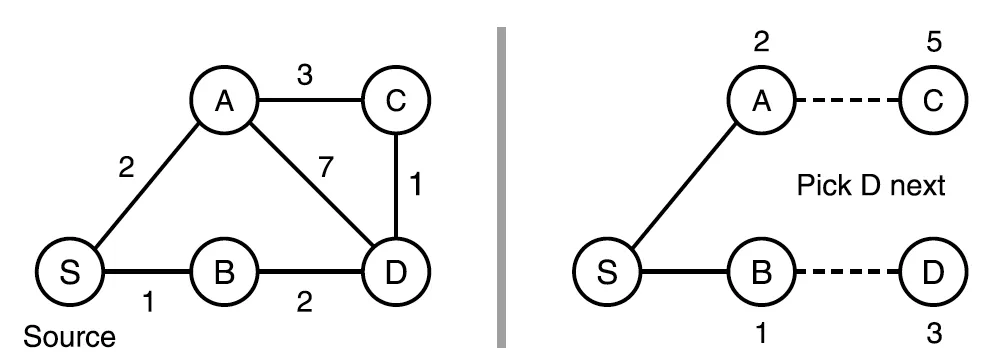
\includegraphics[width=0.8\textwidth]{../assets/ch01/ch01-1_2_网络算法学-009.png}
\end{figure}
图3.9显示，为了检索包含图像的网页，Web客户端通常必须发送一个GET请求以获取页面。如果页面指
定了内联图像，则客户端必须发送单独的请求以检索图像，然后才能显示页面。自然地，应用原则P1会
问，为什么需要单独的请求？为什么Web服务器不能在请求页面时自动下载图像，而不是等待单独的请
求？这应该至少减少一半的往返延迟。
为了测试我们的假设，我们修改了服务器软件以这样做，并测量了结果性能。令我们惊讶的是，我们发
现延迟仅略有改善。
使用基于tcpdump的网络分析器，我们发现了两个原因，说明这种看似改进的想法为何是一个坏主意。
 ● 与TCP的交互：Web传输由TCP协调，如第2章所述。为了避免网络拥塞，TCP从每次往返一个数据
   包开始缓慢增加其速率，然后在收到确认时增加到每次往返两个数据包，依此类推。由于TCP无论
   如何都必须等待确认以增加其速率，因此等待图像的额外请求并未增加延迟。
 ● 与客户端缓存的交互：许多客户端已经缓存了常见的图像，例如.gif文件。让Web服务器单方面下载
   客户端缓存中已有的图像是浪费带宽。请注意，客户端请求图像可以避免这个问题，因为客户端只
   会请求它没有的图像。
从这个案例研究中得到的有用教训是，由于与其他系统部分（如TCP拥塞控制）的交互，改进系统的一
部分可能很困难。
案例研究2：加速基于签名的入侵检测
作为第二个例子，许多网络站点部署了入侵检测系统，例如Snort（2001），它会查找数据包负载中表明
黑客攻击的可疑字符串。例如，字符串“perl.exe”可能表示试图执行perl并在Web服务器上执行任意命
令。对于每个可能匹配的规则，Snort使用Boyer-Moore算法（Cormen等，1990）分别搜索每个字符
串。最坏的情况是一个Web数据包匹配310条规则。简单的剖析使用gprof显示（Fisk和Varghese，
2001），Snort中30%的开销来自字符串搜索。
一个显而易见的应用原则P1似乎是：与其分别搜索每个字符串，不如使用一个集成的搜索算法，在一次
遍历数据包时搜索所有可能的字符串。我们修改了Boyer-Moore算法，使其成为一个集成的Boyer-
Moore算法，可以在一次遍历中搜索所有指定的字符串。在库中实现的新算法比Snort算法快50倍，适用
于完整的Snort数据库。不幸的是，当我们将它集成到Snort中时，我们发现几乎没有改进（Fisk和
Varghese，2001）。我们发现了两个原因。
 ● 多字符串匹配不是跟踪的瓶颈：对于给定的跟踪，很少有数据包匹配多个规则，每个规则包含单独


                                                      22
   的字符串。当我们使用仅包含Web流量（即目标端口为80的流量）的跟踪时，发现了显著的改进。
 ● 缓存效应：集成字符串搜索需要一个数据结构，例如trie，其大小随着被搜索的字符串数量的增长而
   增长。集成集合搜索的最简单方法是将所有规则中的字符串放在一个trie中。然而，当字符串数量超
   过100时，trie无法适应缓存，性能受到影响。因此，系统必须重新实现，以使用考虑硬件（P4）的
   较小集合。
从这个案例研究中得到的有用教训是，所谓的改进可能并未真正针对瓶颈（在跟踪中似乎是单字符串匹
配），并且可能与其他系统部分（数据缓存）发生交互。
3.5.1 八个警示性问题
本着这两个案例研究的精神，这里有八个警示性问题，提醒人们不要滥用这些原则。
Q1：是否值得提高性能？
如果将系统作为产品销售，性能是否是一个主要的卖点？关注性能改进的人可能希望如此，但系统的其
他方面，如易用性、功能性和稳健性，可能更为重要。例如，网络管理产品的用户更关心功能而非性
能。因此，在资源和实现复杂性有限的情况下，我们可能会选择推迟优化，直到需要时再进行。即使性
能很重要，哪个性能指标（例如，延迟、吞吐量、内存）是重要的？
在其他条件相同的情况下，简单性最好。简单的系统更容易理解、调试和维护。另一方面，简单性的定
义随着技术和时间的变化而变化。为了获得较大的性能提升，一定程度的复杂性是值得的。例如，多年
以来，像MPEG这样的图像压缩算法被认为过于复杂，无法在软件或硬件中实现。然而，随着芯片密度
的增加，许多MPEG芯片已经上市。
Q2：这真的是瓶颈吗？
80-20规则表明，大部分性能改进来自于优化系统中的一小部分。一个简单的开始方法是识别我们希望
优化的性能指标的关键瓶颈。一种方法是使用剖析工具，正如我们在案例研究2中所做的那样。
Q3：更改对系统其余部分有何影响？
一个简单的更改可能会加速系统的一部分，但可能对系统的其余部分产生复杂且不可预见的影响。这在
案例研究1中得到了说明。如果一个改进性能但与系统其他部分有太多交互的更改，应该重新考虑。
Q4：初始分析是否表明显著改进？
在进行完整实现之前，快速分析可以指示可能的增益。标准的复杂性分析是有用的。然而，当纳秒至关
重要时，常数因子也很重要。例如，假设分析表明路由器的地址查找是一个瓶颈（例如，因为有快速交

                                                  23
换机使数据传输不是瓶颈）。假设标准算法平均需要15次内存访问，而新算法的最坏情况为3次内存访
问。这表明有5倍的改进，这使得进一步进行变得有趣。
Q5：是否值得添加定制硬件？
随着通用处理器性价比的持续提高，人们很容易倾向于在软件中实现算法，并利用性价比曲线。因此，
如果我们正在考虑一块需要一年时间设计的定制硬件，并且结果的价格性能改进仅为2倍，那么可能不值
得付出努力。另一方面，随着有效的合成工具的出现，硬件设计时间正在缩短。批量生产也可以使定制
芯片的成本（与通用处理器相比）极低。在竞争激烈的市场中，即使只有一年的优势也是很有吸引力
的。这导致公司越来越多地将网络功能放在硅片中。
Q6：是否可以避免协议更改？
多年来，已经有许多提议谴责特定协议效率低下，并提出专门为性能设计的替代协议。例如，在20世纪
80年代，传输协议TCP被认为“慢”，并且明确设计为在硬件中实现的协议XTP（Chesson，1989）。这
激发了研究如何使TCP更快，最终在标准的BSD（Berkeley软件发行版）发布中，Van Jacobson实现了
TCP的快速实现（Clark等，1989）。最近，提出协议更改（例如，标签和流交换）以规避IP查找的需
求，激发了对快速IP查找的研究。
Q7：原型是否确认了最初的承诺？
一旦我们成功回答了所有前面的问题，仍然建议构建一个原型或模拟，并实际测试改进是否真实。这是
因为我们正在处理复杂系统；初始分析很少能捕捉到实践中遇到的所有效应。例如，理解Web图像转储
的想法不会改善延迟（见案例研究1），可能只有在实际实现并通过网络分析器进行测试后才会发现。
一个主要问题是找到一组标准基准测试，以比较标准和新的实现。例如，在通用系统领域，尽管存在一
些分歧，但存在用于浮点性能（例如，Whetstone）或数据库性能（例如，debit-credit）的标准基准测
试。如果有人声称通过差分编码减少Web传输延迟，那么提供一组合理的Web页面作为基准测试以证明
这一主张是什么？如果有人声称拥有一个小存储的IP查找方案，可以使用哪些基准数据库来支持这一断
言？
Q8：如果环境发生变化，性能提升是否会丧失？
即使构建了原型实现，并且基准测试表明性能改进接近初始预测，工作也尚未完成。困难在于，改进可
能特定于所使用的特定平台（可能会改变），并且可能利用了某个基准测试的属性（可能不反映系统将
使用的所有环境）。改进可能仍然是值得的，但某种形式的敏感性分析对于未来仍然有用。
例如，Van Jacobson对BSD网络代码进行了重大优化，使得普通工作站能够饱和100-Mbps FDDI（光
纤分布式数据接口）环。这种优化假设在正常情况下，下一个数据包来自与上一个数据包相同的连接P，
并且序列号比P高1。对于具有数千个同时连接到客户端的服务器，这种假设是否成立？如果数据包通过
                                                        24
网络中的并行链接发送，导致数据包重排序，这种假设是否成立？幸运的是，多年来代码运行良好。尽
管如此，这些问题提醒我们未来可能存在的危险。
3.6 总结
本章介绍了一套高效系统实施的原理。总结可以在图3.1-3.3中找到。这些原理通过从编译器、架构、数
据库、算法和网络中提取的示例进行了说明，以展示其对计算机系统的广泛适用性。Chef Charlie的示例
虽然有些戏谑，但表明这些原理也适用于从餐厅到州政府的通用系统。虽然广泛关注性能，但成本同样
是一个重要指标。可以将问题归结为在给定成本下找到最快的解决方案。优化其他指标（如带宽、存储
和计算）可以归入成本指标之下。
图3.1-3.3中的原理预览可以在后续章节中找到详细解释。前五个原则鼓励系统思维。接下来的五个原则
鼓励对系统模块化进行新的审视。最后五个原则指出了一些加速单个子系统的有用方法。
正如国际象棋策略在玩游戏之前是无聊的，实施原则在没有具体示例的情况下是毫无生气的。鼓励读者
尝试以下练习，这些练习提供了从计算机系统中提取的更多示例。其余章节将对这些原理在网络中的应
用进行探讨。特别是，下一章旨在通过提供一组15个独立的网络问题来吸引读者。


4 原则在行动
系统架构和设计就像任何艺术一样，只能通过实践来学习……只有在操作介质时，可能性的空间才会展
开。
——Carver Mead 和 Lynn Conway
在我把马群聚集起来之后，我现在开始让它们各展其能。——Arnold Toynbee
前一章概述了高效网络协议实现的15条原则。本书的第二部分开始详细研究特定的网络瓶颈，如数据复
制和控制转移。虽然这些原则在后续章节中也会用到，但这些章节的重点是所考察的具体瓶颈。鉴于网
络算法学既是一种思维方式，也是一套技术，通过在小型的、自成一体的但非平凡的网络问题上应用这
些原则来结束第一部分似乎是有用的。
因此，本章提供了在解决特定网络问题时应用这些原则的示例。这些示例来自真实问题，其中一些解决
方案已在实际产品中使用。与后续章节不同，本章不是一个新材料的集合，后面跟着一系列练习。相
反，本章可以被认为是一系列扩展的练习。
在4.1到4.15节中，描述了15个问题，并对每个问题进行了说明。每个问题后面都有一个提示，建议使用
特定的原则，然后是一个解决方案概述。每个解决方案后面还有一些练习。在关于本章主题的课程和研
讨会上，听众喜欢在得到一些提示后自己发明解决方案（而不是直接看到最终解决方案）。

                                                  25
快速参考指南
在一个理想的世界里，每个问题都应该对每个读者都有有趣的地方。然而，对于时间紧迫的读者，这里
有一些指导。硬件设计师如果想尝试一些问题，可以尝试设计一个以太网监控器（第4.4节）或对长标识
符进行二分搜索（第4.14节）。系统人员如果想了解系统思维如何巧妙地解决算法专业知识的问题，可以
尝试解决应用设备通道问题（第4.1节）或压缩连接表问题（第4.11节）。算法设计师可能会对识别资源
消耗者问题（第4.10节）和使用协议设计变更来简化链路状态路由中的实现问题（第4.8节）感兴趣。
4.1 应用设备通道的缓冲区验证
通常，应用程序只能通过操作系统内核发送网络数据，并且只有内核可以与网络适配器通信。这种限制
防止了不同应用程序恶意或意外地写入或读取彼此的数据。然而，通过内核进行通信会增加系统调用形
式的开销（见第2章）。在应用设备通道（ADCs）中，允许应用程序通过直接写入网络适配器的内存来
发送和接收网络数据。更多细节请参见第5章。一种无需内核调解的保护机制是让内核为每个应用程序设
置一组有效的内存页。然后，网络适配器必须确保应用程序的数据只能从有效页集合中的内存发送和接
收。
例如，在图4.1中，应用程序P被允许从有效页集合X、Y、...、L、A中发送和接收数据。假设应用程序P
向适配器发出请求，将下一个数据包接收到的缓冲区放入页A中。由于此请求是直接发送到适配器的，内
核无法检查这是否是P的有效缓冲区。相反，适配器必须通过确保A在有效页集合中来验证此请求。如果
适配器不执行此检查，应用程序P可能会提供一个属于其他应用程序的无效页，适配器会将P的数据写入
错误的页中。这种检查需求导致了以下问题。




In application device channels, the network adaptor is given a set of valid pages (X,Y,L,A, etc.)
for a given application P. When application P makes a request to receive data into page A, the
adaptor must check if A is in the valid list before allowing the receive.

                                                                                                    26
问题
当应用程序P执行接收操作时，适配器必须验证该页是否属于P的有效页集合。如果页集合被组织成一个
线性列表（Druschel等人，1994年），那么验证的成本为O(n)，其中n是集合中的页数。例如，在图4.1
中，由于A位于有效页列表的末尾，适配器必须在找到A之前遍历整个列表。如果n很大，这可能会非常
昂贵，并减慢适配器发送和接收数据包的速率。如何加快验证过程？
提示：减少验证复杂性的一个好方法是使用比列表更好的数据结构（P15）。你会选择哪种数据结构？然
而，通过系统思维并在接口中传递提示（P9），可以进一步改善最坏情况的行为并减小常数因子。
算法设计者会立即考虑将有效页集合实现为哈希表而不是列表。这提供了O(1)的平均搜索时间。哈希有两
个缺点：（1）具有小碰撞概率的好哈希函数在计算上代价昂贵；（2）哈希不提供良好的最坏情况界
限。二分搜索确实提供了对数最坏情况搜索时间，但如果页集合很大且数据包传输速率很高，这会很昂
贵（还需要保持集合有序）。相反，我们用索引数组查找替换哈希表查找，如下所示（在继续阅读之前
尝试使用P9）。
解决方案




Finessing the need for a hash table lookup by passing a handle across the interface between the
application and adaptor.
适配器将每个应用程序的有效页集合存储在一个数组中，如图4.2所示。这个数组只有在应用程序的有效
页集合被内核更新时才会更新。当应用程序请求将数据接收到页A时，它还会向适配器传递一个句柄
（P9）。该句柄是数组中存储A的位置的索引。适配器可以使用这个来快速确认接收请求中的页是否与
句柄中存储的页匹配。验证的成本是一个边界检查（查看句柄是否为有效索引）、一次数组查找和一次
比较。
练习
                                                                                             27
 ● 句柄是一个提示还是一个提示？让我们调用原则P1：如果这是一个句柄，为什么在接口中传递页号
   （例如A）？为什么在接口中移除页号可以稍微加快确认任务的速度？
 ● 通常需要使用哈希表搜索P来找到与应用程序P对应的数组。这削弱了摆脱哈希表搜索以检查页是否
   有效的论点——除非当然，P的哈希搜索也可以被巧妙地处理。如何做到这一点？
4.2 异步传输模式流量控制的调度器
在异步传输模式（ATM）中，ATM适配器可能有数百个同时的虚拟电路（VCs），这些虚拟电路可以发
送数据（称为信元）。每个VC通常以某种方式受到流量控制，以限制其发送速率。例如，在基于速率的
流量控制中，VC可能会在固定的时间间隔内接收发送信元的信用。另一方面，在基于信用的流量控制中
（Kung等人，1994年；Ozveren等人，1994年），当路径上的缓冲区释放时，下一个节点可能会发送信
用。




An ATM VC is eligible to send data if it is active (has some outstanding cells to send in the
queue shown below the VC) and has credits (shown by gray dots above the VC). The problem is
to select the next eligible VC in some fair manner without stepping through VCs that are
ineligible.
因此，在图4.3中，适配器有一个表，其中保存了VC的状态。已经建立了四个VC（1、3、5、7）。其
中，只有VC 1、5和7有一些信元要发送。最后，只有VC 1和7有信用可以发送信元。因此，适配器接下
来要发送的信元应该是来自符合条件的VC之一：1或7。从符合条件的VC中选择下一个信元应该公平地进
行，例如，以轮询的方式进行。如果适配器选择从VC 7发送一个信元，适配器会将VC 7的信用减少到
1。由于没有更多的信元要发送，VC 7现在变得不合格。选择下一个符合条件的VC会导致以下问题。
问题

                                                                                           28
一个简单的调度器可能会循环遍历VC数组，寻找一个符合条件的VC。如果许多VC都不符合条件，这可
能非常低效，因为调度器可能不得不遍历几个不符合条件的VC才能从一个符合条件的VC发送一个信元。
如何避免这种低效？
提示：考虑调用P12来添加一些额外的状态以加快调度器主循环的速度。你可以添加什么状态来避免遍历
不符合条件的VC？如何有效地维护这种状态？
解决方案




Maintaining a list of eligible VCs to speed up the scheduler main loop.
除了图4.3中的VC表之外，还维护一个符合条件的VC列表（图4.4）。唯一的问题是如何有效地维护这种
状态。这是使用P12的主要困难。如果状态维护成本过高，那么添加的状态就是一种负担而不是资产。回
想一下，VC符合条件是指它既有信元要发送又有信用。因此，VC在服务后如果没有信元要发送或没有更
多信用，就会从列表中移除；否则，VC会被添加到列表的尾部，以确保公平性。VC会在空VC信元队列
中到达一个信元并且这个（空的）队列也有信用，或者当VC没有信用并接收到信用更新时，被添加到列
表的尾部。
练习
 ● 如何确保一个VC不会被多次添加到符合条件的列表中？
 ● 这种方案是否可以推广，以允许某些VC根据管理者分配的权重获得比其他VC更多的发送机会？



4.3 使用Dijkstra算法进行路由计算
路由器S如何决定如何将数据包路由到给定目的地D？网络中的每条链路都被标记了一个成本，像S这样
的路由器通常会计算到本地域内目的地的最短（即最低成本）路径。假设成本是一个小整数。回想一下
第2章中提到的，在一个域内最常用的路由协议是基于链路状态路由的OSPF（开放最短路径优先）。
在链路状态路由中，子网中的每个路由器都会发送一个链路状态包（LSP），列出其与所有邻居的链路。
每个LSP都会被发送到子网中的每个其他路由器。每个路由器使用一个原始的洪泛协议（Perlman，1992
年）通过其LSP向其他路由器发送信息。一旦每个路由器从每个路由器接收到一个LSP，那么每个路由器
                                                                     29
就拥有了网络的完整地图。假设拓扑结构保持稳定，每个路由器现在可以使用标准的短路径算法（如
Dijkstra算法（Cormen等人，1990年））计算到网络中每个其他节点的最短路径。
在图4.5中，源S希望计算到网络中所有其他节点（A、B、C、D）的最短路径树。网络在图4.5的左框中
显示，链路编号带有其成本。在Dijkstra算法中，S首先将自己放入最短路径树中。S还会更新到达其直接
邻居（例如B、A）的成本。在每次迭代中，Dijkstra算法会将当前树中最接近的节点添加到树中。这个
新添加节点的邻居的成本会被更新。这个过程重复，直到网络中的所有节点都属于树。




In Dijkstra’s algorithm the source S builds a shortest-path tree rooted at S. At each stage, the
closest node not in the tree is added to the tree.
例如，在图4.5中，在添加S之后，算法选择B，然后选择A。在这次迭代中，树如图4.5右框所示。实线
显示了现有的树，虚线显示了到尚未在树中的节点的最佳当前连接。因此，由于A的成本为2，并且有一
条成本为3的链路从A到C，C被标记为5。类似地，D被标记为通过B的路径的成本为3。在下一次迭代
中，算法选择D作为尚未在树中的最小成本节点。然后使用通过D的路径更新C的成本。最后，在最后一
次迭代中，C被添加到树中。
这个教科书解决方案需要在每次迭代时确定一个不在树中的最小成本节点。跟踪动态变化集合中最小值
元素的标准数据结构是优先队列。这导致了以下问题。
问题
Dijkstra算法在N次迭代中需要一个优先队列，其中N是网络节点的数量。最好的通用优先队列，如堆
（Cormen等人，1990年），找到最小元素的成本为O(log N)。这意味着总运行时间为O(N log N)时间。
对于大型网络，这可能导致对故障和其他网络拓扑变化的响应缓慢。如何加快路由计算速度？
提示：考虑利用链路成本是小整数这一事实（P14），使用数组来表示节点的当前成本。如何有效地找到
下一个最小成本节点以包含在最短路径树中？
解决方案
可以利用链路成本是小整数这一事实来构建一个基于桶排序的优先队列（P14）。假设最大链路成本为
MaxLinkCost。因此，路径的最大成本不会超过Diam*MaxLinkCost，其中Diam是网络的直径。假设
                                                                                               30
Diam也是一个小整数。因此，可以想象使用一个数组，每个可能的成本c在范围1... Diam *
MaxLinkCost中都有一个位置。如果在Dijkstra算法的过程中节点X的成本从c变为c'，则节点X将从c的列
表中移除并添加到c'的列表中。但是如何找到最小元素呢？这可以通过初始化一个名为CurrentMin的指
针来实现，指向0（对应于S的成本）。每次算法希望找到不在树中的最小成本节点时，CurrentMin递增
1，直到到达一个包含非空列表的数组位置。然后可以将该列表中的任何节点添加到树中。算法的成本为
O(N + Diam * MaxLinkCost)，因为在推进CurrentMin时最多只能进行数组大小的操作。对于大型N和
小Diam和MaxLinkCost值，这可能比N log N要好得多。
能够有效使用前面描述的基于桶排序的优先队列的一个关键因素是，节点成本始终领先于CurrentMin的
值。这是一个单调性条件。如果不是这样，算法将在每次迭代时从1开始检查最小值，而不是从上一次
CurrentMin的值开始，并且永远不会回退。对于Dijkstra算法来说，这个单调性条件是相当明显的，因为
尚未在树中的节点的成本必须大于已在树中的节点的成本。




Using a priority queue based on bucket sorting to speed up Dijkstra’s algorithm.
图4.6显示了在A被添加到树中之后基于桶排序优先队列的状态。这对应于图4.5的右框。此时，
CurrentMin=2，这是A的成本。在下一次迭代中，CurrentMin将递增到3，D将被添加到树中。这将导致
C的成本降低到4。因此，我们将C从位置5的列表中移除，并将其添加到位置4的空列表中。然后
CurrentMin递增到4，C被添加到树中。
练习
 ● 如何有效地将一个节点从一个列表中移除并添加到另一个较早的列表中？
 ● 在图4.6中，算法如何知道在将C添加到树中后可以终止，而不是推进到长数组的末尾？
 ● 在实际网络中，故障会导致直径发生很大变化，因为故障可能会显著增加网络的直径。例如，在一
   个轮式拓扑中，所有N个节点通过一个中心辐条节点的直径为2；如果中心辐条节点发生故障，直径
   将增加到N/2。实际上，直径通常很小。这是否会导致在确定数组大小时出现问题？
 ● 是否可以通过用大小为MaxLinkCost的循环数组替换图4.6中的线性数组来完全规避直径问题？解释
   一下。这种解决方案被称为Dial算法（Ahuja等人，1993年）。

                                                                              31
4.4 使用桥接硬件的以太网监控器
Alyssa P. Hacker 在 Acme Networks 工作，她知道 Acme 发明的以太网桥。桥是一种可以连接以太网
的设备。为了将数据包从一个以太网转发到另一个以太网，桥必须以高速度在以太网数据包中查找48位
目标地址。
Alyssa 决定将桥改造成一个以太网流量监控器，该监控器将被动监听以太网并生成有关流量模式的统计
信息。营销人员告诉她，她需要监控任意源-目的地址对之间的流量。因此，对于每对活动的源-目的地
址对，如A、B，Alyssa必须维护一个变量PA,B，用于测量自监控器启动以来从A发送到B的数据包数量。
当从A发送到B的数据包到达时，监控器（监听电缆上发送的所有数据包）将捕获数据包的副本。如果源
是A且目的地是B，监控器应增加PA,B。问题在于如何在64微秒内完成这一任务，这是以太网上最小数据
包间隔时间。瓶颈在于查找与一对48位地址A、B相关联的状态PA,B。
幸运的是，桥接硬件具有一个出色的查找硬件引擎，可以在1.4微秒内查找单个48位地址的状态。可以表
示为Lookup(X,D)，其中X是48位键，D是要搜索的数据库。调用将在1.4微秒内返回与X相关联的状态，
适用于少于64,000个键的数据库。Alyssa需要解决以下问题。
问题
监控器需要在从A到B的数据包到达时更新PA,B的状态。监控器有一个只能查找单个地址的查找引擎，而
不是地址对。Alyssa如何使用现有的引擎来查找地址对？问题如图4.7所示。




Adapting an engine that does destination lookups to doing source-destination lookups
提示：问题要求利用现有的桥接硬件（P4c）。由于1.4微秒远小于64微秒，设计可以承担多个硬件查找
的成本。如何使用三个查找将96位查找转换为48位查找？
一个简单的解决方案是使用两个查找将源A和目的地B转换为较小的（<24位）索引IA和IB。然后可以使
用这两个索引来查找存储AB状态的二维数组。这只需要两个硬件查找加上一次内存访问，但可能需要大
量内存。如果可能有20,000个活动的源-目的地址对，而只有1000个可能的源和1000个可能的目的地，
那么数组必须包含一百万个条目。如何使所需的内存量与实际活动的源-目的地址对的数量成正比？


                                                                                   32
解决方案
如前所述，首先使用一次查找将源A和目的地B分别转换为较小的（<24位）索引IA和IB。然后使用第三
次查找将IA和IB映射到AB状态。解决方案如图4.8所示。第三次查找有效地压缩了简单解决方案中的二维
数组。这个解决方案是由Mark Kempf和Mike Soha提出的。




Converting a 96-bit lookup into a 48-bit lookup by first converting each 48-bit address into a
24-bit index and concatenating the indices.
练习
 ● 是否可以使用仅两个桥接硬件查找而不需要额外的内存来解决这个问题？
 ● 活动的源-目的地址对可能会随着时间的推移而变化，因为某些地址对可能在很长一段时间内停止通
   信。如何在不保留自监控器启动以来所有通信过的地址对的每个可能地址对的状态的情况下处理这
   种情况？
4.5 x-kernel中的解复用
x-kernel（Hutchinson和Peterson，1991年）提供了一个用于主机协议实现的软件基础设施。x-kernel
系统支持许多必需的协议功能。一个常见的必需功能是协议解复用。例如，当互联网路由层IP接收到一
个数据包时，它必须使用协议字段来确定数据包接下来应该发送到TCP（传输控制协议）还是UDP（用
户数据报协议）。
大多数协议确实基于协议头中的某个标识符进行解复用。这些标识符在不同的协议中可以有不同的长
度。例如，以太网类型字段可以是5字节，而TCP端口号是2字节长。因此，x-kernel允许基于可变长度
协议标识符进行解复用。当系统初始化时，协议例程可以向x-kernel注册标识符与目标协议之间的映
射。运行时，当数据包到达时，协议例程可以从数据包中提取协议标识符，并查询x-kernel解复用例程
以获取目标协议。由于数据包可能以高速到达，解复用例程应该快速。这导致了以下问题。
问题
                                                                                                 33
通常，最快的查找方法是使用哈希表。如图4.9所示，这需要对标识符K进行某种哈希函数计算以生成哈
希索引，使用该索引访问哈希表，并将存储在哈希表条目中的键L与K进行比较。如果匹配，则解复用例
程可以检索与键L相关联的目标协议。假设已经选择了哈希函数以使冲突不频繁。




Demultiplexing in the x-kernel is done by hashing the protocol identifier K and (potentially) using
a byte-by-byte comparison with the key L stored at the hash table entry.
然而，由于标识符的长度是任意数量的字节，比较例程通常必须逐字节进行比较。但是，假设最常见的
情况是4字节标识符，这是机器字的大小。在这种情况下，使用字比较会更高效。因此，目标是利用高效
的字比较（P4c）来优化预期情况（P11）。如何在仍然处理任意协议的同时做到这一点？
提示：注意，如果x-kernel需要解复用一个3字节标识符，它必须使用逐字节比较例程；如果x-kernel需
要解复用一个4字节标识符，并且4字节是机器字大小，它可以使用字比较。第一个可以利用的自由度是
为最常见的情况（例如，字比较、长字比较）提供不同的比较例程，并为每种协议提供一个默认的比较
例程，该例程使用逐字节比较。这样做是以额外的空间换取时间（P4b）。然而，为了正确性，了解每种
协议应使用哪种比较例程是很重要的。考虑调用原则P9在接口中传递提示和P2a进行一些预计算。
解决方案
每个协议在系统初始化时都必须向x-kernel声明其标识符和目标协议。此时，每个协议都可以预先声明
其标识符长度，因此x-kernel可以为每个协议使用专门的比较例程。实际上，信息是在客户端协议和x-
kernel之间传递的（P9），并且在早期（P2a）进行。假设x-kernel为每个客户端协议都有一个单独的哈
希表，并且x-kernel知道每个客户端的上下文，以便使用该客户端的专用代码。
练习
 ● 在你的机器上编写字节逐字节和字比较的代码，并进行大量两种类型的比较，比较每种类型的总体
   时间。
 ● 在早期的ADC解决方案中，通过传递索引（而不是标识符长度）来简化哈希表查找。为什么在这种
   情况下这种方法可能比较困难？
4.6 带节点压缩的Trie树
                                                                                                34
Trie storing three keys. Notice the wasted space in the trie nodes.
Trie是一种树形数据结构，其中每个节点是一个包含M个元素的数组。\begin{figure}[htbp]
\centering
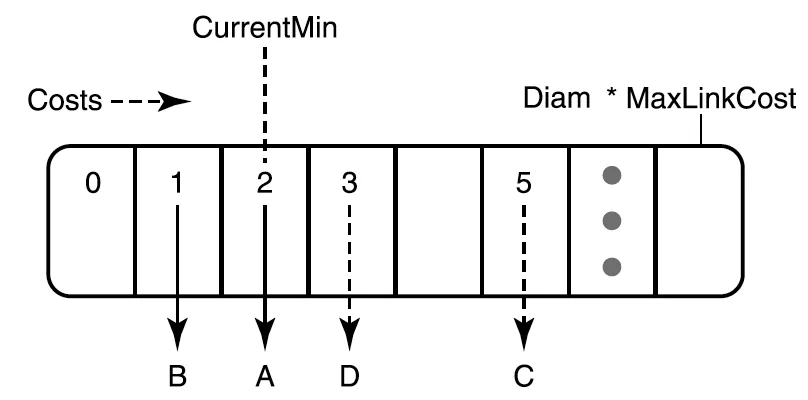
\includegraphics[width=0.8\textwidth]{../assets/ch01/ch01-1_2_网络算法学-010.png}
\end{figure}
图4.10展示了一个简单的例子，
M=8。每个数组可以存储一个键（例如，图4.10中的KEY 1、KEY 2或KEY 3）或指向另一个Trie节点的
指针（例如，图4.10顶部Trie节点的第一个元素，即根节点）。Trie用于搜索输入字符串的精确匹配（和
最长前缀匹配）。在网络中，Trie用于各种任务，如IP地址查找（第11章）、桥接查找（第10章）和解复
用过滤器（第8章）。
具体的Trie算法在这里并不重要。我们只需要知道如何搜索Trie。设 c = log2 M 为Trie的块大小。为
了搜索Trie，首先将输入字符串分成大小为c的块。搜索从最高有效位开始，使用连续的块来索引Trie的
                                                  ​




节点，从根节点开始。当搜索使用块j索引当前Trie节点的位置i时，位置i可以包含一个指针或一个键。如
果位置i包含一个非空指针到节点N，则搜索继续在节点N中使用块j+1；否则，搜索终止。
总结来说，每个节点是一个指针或键的数组，搜索过程需要索引这些数组。然而，如果许多Trie节点是稀
疏的，就会浪费大量空间（P1）。例如，在图4.10中，16个位置中只有4个包含有用信息。在最坏的情况
下，每个Trie节点可能包含1个指针或键，并且可能存在M倍的浪费内存。假设 M ≤ 32 ，即使M这么
小，也可能导致内存增加32倍，这会大大增加设计成本。
一个显而易见的解决方案是用线性列表替换每个Trie节点，形式为(i, val)，其中val是节点中位置i的非空
值（指针或键）。例如，图4.10中的根Trie节点可以被替换为列表 (1, ptr1); (7, KEY 1) ，其中ptr1
是指向底部Trie节点的指针。不幸的是，这可能会使Trie搜索速度减慢M倍，因为每个Trie节点的搜索可
能现在需要在M个位置的列表中进行搜索，而不是单个索引操作。这导致了以下问题。
问题
如何压缩Trie节点以去除空指针而不显著减慢搜索速度？
提示：尽管压缩了节点，数组索引仍需高效。如果节点被压缩，如何表示哪些数组元素被移除的信息？
考虑利用M较小这一事实（P14和P4a）。
解决方案
                                                                 35
由于 M < 32 ，一个大小为32的位图可以轻松地放入一个计算机字中（P14和P4a）。因此，在添加了
一个位图后，空指针被移除，位图中零位表示原始位置的空指针。如\begin{figure}[htbp]
\centering
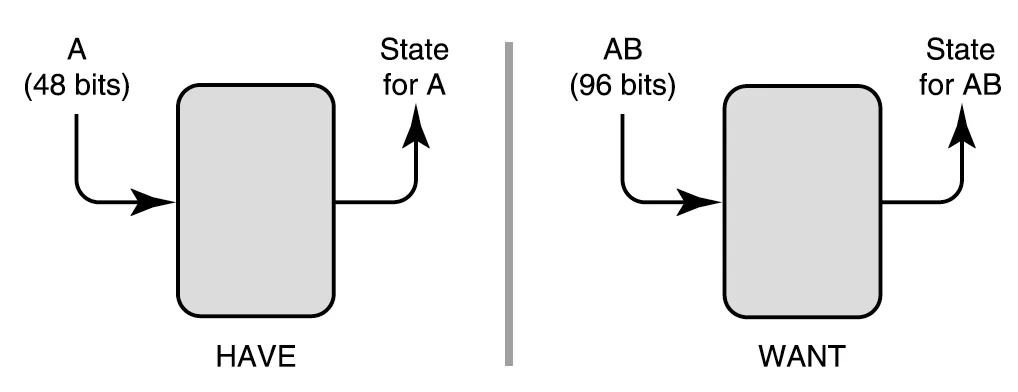
\includegraphics[width=0.8\textwidth]{../assets/ch01/ch01-1_2_网络算法学-011.png}
\end{figure}
图4.11所示，Trie节点现在可以被替
换为一个位图和一个压缩的Trie节点。压缩的Trie节点是一个仅包含原始节点中非空值的数组。因此，在
图4.11中，原始根Trie节点（顶部）已被替换为压缩的Trie节点（底部）。位图在第一个和第七个位置包
含1，表示根节点包含非空值。压缩后的数组现在只包含两个元素，第一个指针和KEY 3。这仍然引出了
一个问题：如何搜索Trie节点？




Compressing a trie node using a bitmap and bit counting to efficiently translate from an
uncompressed index to a compressed index.
由于未压缩和压缩的节点都是数组，并且搜索过程从索引I开始进入未压缩节点，搜索过程必须咨询位图
以将未压缩索引I转换为压缩索引C进入压缩节点。例如，如果I是1，则C应该是1；如果I是7，则C应该是
2。如果I是其他值，则C应该是0，表示只有一个空指针。
幸运的是，从I到C的转换可以通过以下方式轻松完成。如果位图中的位置I包含0，则C=0。否则，C是位
图中前I位中1的数量。因此，如果 I = 7 ，则 C = 2 ，因为位图中的前七位中有两个位被设置。
练习
 ● 如何使用表查找（P14，P2a）来加速软件中计算位图中1的数量？这是否一定需要第三次内存引用？
 ● 假设位图很大（例如， M = 64K ）。在硬件或软件中计算这样一个大位图中1的数量似乎慢得不
   可思议。你能找到一种方法，仅使用一次额外的内存访问来加速大位图中1的计算吗？这在第11章中
   将非常有用。
4.7 路由器中的数据包过滤

                                                                                      36
第12章描述了在路由器上设置资源以处理需要性能保证的流量（如视频）的协议。这些协议使用数据包
过滤器的概念，有时称为分类器。因此，在\begin{figure}[htbp]
\centering
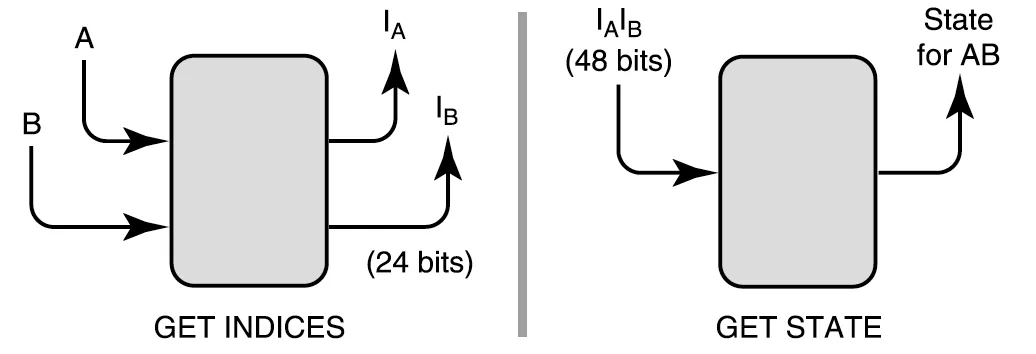
\includegraphics[width=0.8\textwidth]{../assets/ch01/ch01-1_2_网络算法学-012.png}
\end{figure}
图4.12中，连接到路由器的每个接收器可能指定一个数据包过
滤器，描述其希望接收的数据包。例如，在图4.12中，接收器1可能希望接收NBC，这由过滤器4指定。
每个过滤器都是对NBC发送的视频数据包的字段的某种规范。例如，NBC可能由使用德国NBC发射机的
源地址和指定的TCP目标和源端口号的数据包指定。
同样，在图4.12中，接收器m可能希望接收ABC Sports和CNN，这分别由过滤器1和7描述。数据包以高
速到达路由器，并且必须发送给所有请求该数据包的接收器。例如，接收器1和2可能都希望接收NBC。
这导致了以下问题。




Packet filtering in a router may require a slow linear scan of all filters followed by making a copy
of the packet for all filters that match.
问题
每个到达的数据包必须与所有过滤器匹配，并发送给所有匹配的接收器。如果过滤器数量很大，简单的
线性扫描所有过滤器会很昂贵。假设过滤器数量超过一千。如何加快这一昂贵的过程？
提示：人们可能会考虑通过缓存（P11a）来优化预期情况。然而，为什么在这种情况下缓存很困难？考
虑在数据包头中添加一个字段（P10），以使缓存更容易。理想情况下，这个字段应该添加到哪个协议
层？添加一个不需要全局标准化标识符的固定众所周知的字段对于每个可能的视频类型是不够的，因为
过滤器可能基于其他字段，如源地址。假设你添加的字段不需要全局标准化的标识符。发送方必须确保
什么？
解决方案
缓存（P11a），系统设计师的老工具，在这个问题上并不十分直接。通常，缓存存储输入a和某些输出
f(a)之间的映射。然后，缓存由形式为(a,f(a))的对组成。这些对存储在一个数据库中，以a的值作为键。
该数据库可以实现为一个哈希表（在软件中）或内容可寻址存储器（在硬件中）。给定输入a并需要计算
                                                                                                   37
f(a)，首先检查数据库中是否存在a。如果存在，则快速路径退出并返回现有的f(a)。如果不存在，则使用
某种（可能昂贵的）计算来计算f(a)，并将对(a,f(a))插入缓存数据库。随后具有值a的输入可以非常快速
地计算。
在数据包过滤问题中，目标是计算与数据包P相关联的接收器集合。问题是输出是P的（可能很大的）数
据包头字段集合的函数。因此，要使用缓存，必须存储P的头部的大部分与接收器集合的映射。存储64字
节数据包头部与接收器集合的映射是一个昂贵的提议。这在时间上昂贵，因为搜索缓存可能需要更长时
间，因为键很宽。这显然在存储上也昂贵。更大的存储需求反过来意味着给定缓存大小可以缓存的映射
更少，这导致缓存命中率较低。
理想的情况是缓存一个或两个数据包字段与输出接收器集合之间的映射。这将加快缓存搜索速度并提高
缓存命中率。这些字段最好也在路由头中，路由器无论如何都会检查这些字段。问题是可能没有这样一
个唯一指纹数据包P的字段。
然而，假设我们是设计路由协议的设计师。我们可以向路由头添加一个字段。问题似乎很简单，如果我
们可以为每个可能的流分配一个唯一的全球标识符。例如，如果我们可以为NBC分配标识符1，为ABC分
配标识符2，为CNN分配标识符3，那么我们可以使用标识符作为键进行缓存。这样的解决方案将需要某
种全球标准委员会负责命名每个应用流。即使这可以实现，接收器过滤器可能要求所有NBC数据包来自
某个源，并且过滤器可能依赖于其他数据包字段。这导致了以下最终想法。




Adding a flow identifier (which is unique only with respect to a source) can speed up packet
filtering.
更改路由头以添加一个流标识符F（\begin{figure}[htbp]
\centering
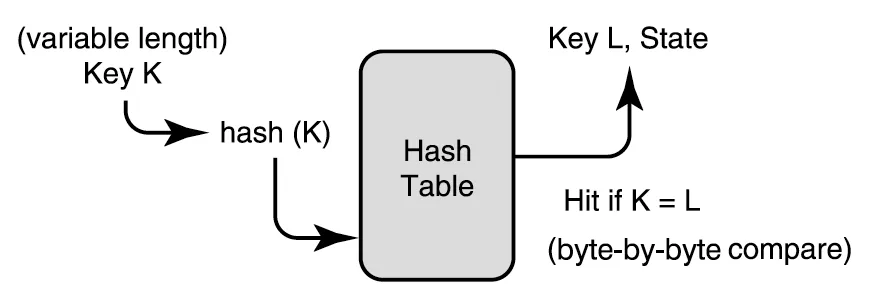
\includegraphics[width=0.8\textwidth]{../assets/ch01/ch01-1_2_网络算法学-013.png}
\end{figure}
图4.13），其含义取决于源。换句话说，不同的源可以使用相同的流
标识符，因为是源和流标识符的组合是唯一的。因此，不需要全球标准化（或其他全球协调）流标识
                                                                                          38
符。流标识符只是源维护的一个本地计数器。想法是发送应用程序可以向路由层请求一个流标识符。这
个标识符被添加到该应用程序所有数据包的路由头中。
通常，当应用程序数据包第一次到达时，路由器会进行（缓慢的）线性搜索，以确定与数据包头相关联
的接收器集合。由于标识符在源之间不唯一，路由器会缓存使用源地址和流标识符的连接作为键的映
射。显然，正确性取决于发送应用程序在不更改可能影响过滤器的数据包字段的情况下不更改数据包中
的流标识符。
练习
 ● 如果源崩溃并在没有记住它为不同应用程序分配了哪些标识符的情况下重新启动，会发生什么？当
   接收器添加新过滤器时会发生什么？如何解决这些问题？
 ● 在当前解决方案中，流标识符被用作提示（第3章），而不是提示。如果将流标识符-源地址对视为
   提示而不是提示，会带来哪些额外成本？
4.8 避免LSP的碎片化
以下问题实际上出现在OSI和OSPF（Perlman，1992年）链路状态路由协议的设计过程中。这个问题是
关于协议设计的，而不是协议实现（一旦设计确定）。尽管如此，它说明了设计选择如何极大地影响实
现性能。
第2章和第4.3节描述了链路状态路由。回想一下，在链路状态路由中，路由器必须发送一个LSP，列出
其所有邻居。链路状态协议包括两个独立的过程。第一个是更新过程，它使用依赖于每个LSP的唯一序列
号的可靠洪泛协议从一个路由器向另一个路由器发送LSP。序列号用于拒绝重复的LSP副本。每当路由器
从源S接收到编号为x的新LSP时，路由器将记住编号x，并拒绝来自S的任何后续具有序列号x的LSP。在
更新过程完成其工作后，每个路由器上的决策过程将应用Dijkstra算法到由LSP形成的网络图。
虽然路由器可能只有少量路由器邻居，但路由器可能有大量直接连接到同一局域网的主机计算机（端节
点）。例如，在\begin{figure}[htbp]
\centering
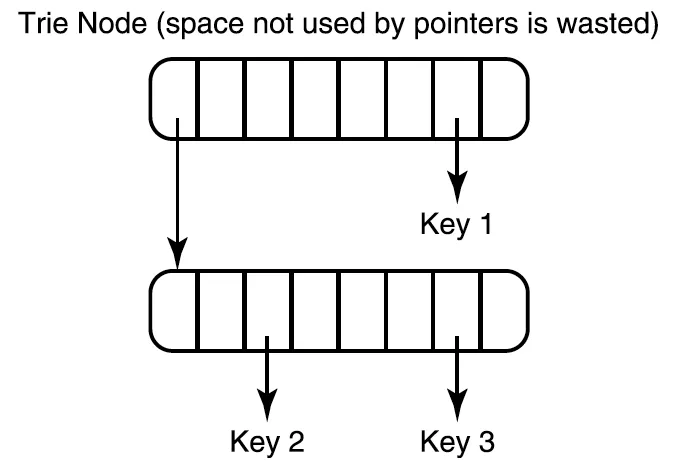
\includegraphics[width=0.8\textwidth]{../assets/ch01/ch01-1_2_网络算法学-014.png}
\end{figure}
图4.14中，路由器R1有500个端节点邻居E1...E500。大型局域网甚至可能有更多的端节
点。这导致了以下问题。




                                                    39
The LSP of router R1 (with even 500 endnode neighbors) may be too large to fit into a data link
frame. Without a clever idea, this would require inefficient fragmentation and reassembly of the
LSP at every hop.
问题
每个端节点占用8字节（6字节用于标识端节点，2字节用于成本信息），LSP可能会非常大（对于5000
个端节点为40,000字节）。这对于许多常用数据链路上的最大帧大小来说太4.15大了。例如，以太网的
最大帧大小为1500字节，FDDI指定最大帧大小为4500字节。这意味着大LSP必须在每个跃点上被分割成
许多数据链路帧，并在每个路由器上重新组装后才能继续发送。这需要在每个跃点上进行昂贵的重新组
装过程，以确定是否已接收到LSP的所有部分。
这还会增加链路状态传播的延迟。假设每个LSP可以装入M个数据链路帧，网络的直径为D，发送数据链
路帧的时间为1个时间单位。那么，使用逐跳重新组装时，LSP的传播时间为D·M。如果路由器不必在每
个跃点等待重新组装每个LSP，则传播延迟仅为M+D。当设计链路状态协议时，实现者发现了这些问题
（Perlman，1992年）。
另一方面，似乎不可能独立传播片段，因为LSP携带一个对更新过程至关重要的单一序列号。简单地将序
列号复制到每个片段中是无济于事的，因为这将导致后续片段被拒绝，因为它们具有与第一个片段相同
的序列号。问题是使不可能成为可能，通过空间上的计算转移来避免逐跳碎片化。允许对LSP路由协议进
行更改。
提示：所有5000个端节点的信息是否必须位于同一个LSP中？考虑调用P3c来转移空间上的计算。
解决方案
如果原始R1的LSP的各个片段要独立传播而不进行逐跳重新组装，则每个片段必须是一个单独的LSP，并
具有单独的序列号。这个关键观察导致了以下巧妙的方法。




Avoiding hop-by-hop fragmentation by dividing a large router into pseudorouters.

                                                                                                   40
修改链路状态路由协议，允许任何路由器R1成为多个伪路由器R1a、R1b、R1c（见\begin{figure}[htbp]
\centering
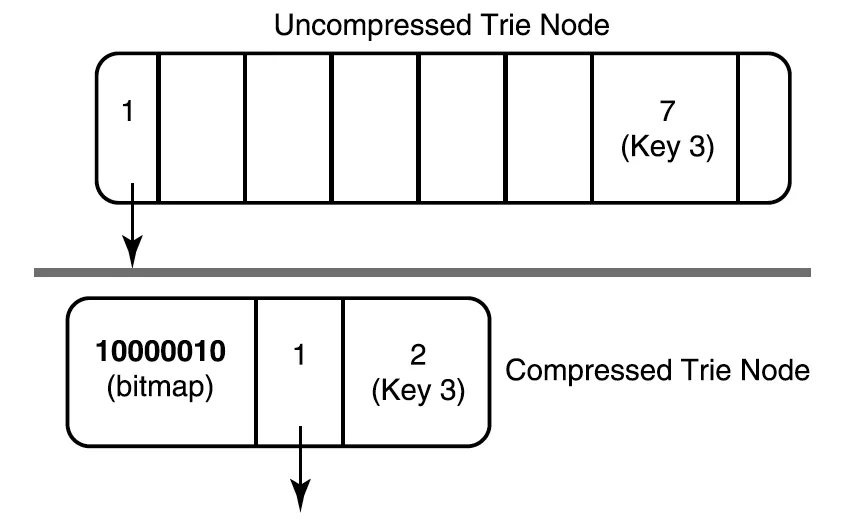
\includegraphics[width=0.8\textwidth]{../assets/ch01/ch01-1_2_网络算法学-015.png}
\end{figure}
图4.15）。原始的端节
点集合被分配到这些伪路由器中，因此每个伪路由器的LSP可以装入大多数数据链路帧而无需碎片化。例
如，如果大多数数据链路大小至少为576字节，则大约72个端节点可以装入一个数据链路帧。
如何实现伪路由器的概念？在原始LSP传播中，每个路由器都有一个6字节的ID，放置在所有由该路由器
发送的LSP中。为了允许伪路由器，我们更改协议，使LSP携带一个7字节ID（6字节路由器ID + 1字节伪
路由器ID）。伪路由器ID可以由实际包含所有伪路由器的路由器分配。通过允许每个路由器有256个伪路
由器，大约18,000个端节点可以支持每个路由器。
虽然LSP传播将伪路由器视为单独的实体，但重要的是路由计算将不同的伪路由器视为同一个路由器。毕
竟，端节点都直接连接到R1。但这很容易做到，因为所有以相同前6字节开头的LSP都可以被识别为来自
同一个路由器。
总之，主要思想是通过让源将原始LSP碎片化为独立的LSP来转移空间上的计算（P3c），而不是让每个
数据链路进行碎片化。这是一个很好的系统思维示例。不用说，实现者比原始方法更喜欢这个解决方案
（由Radia Perlman发明）。
练习
● 路由器如何分配端节点到伪路由器？如果路由器最初有很多端节点（因此有很多伪路由器），然后
  大多数端节点死亡，会发生什么？这可能会留下许多伪路由器，每个伪路由器只有少数端节点。为
  什么这不好，如何解决？
● 如第3章中描述的放宽一致性示例一样，这种解决方案可能导致一些意外的（但不是很严重的）临时
  不一致。假设解决了前面的练习，描述一个场景，在该场景中，某个路由器（例如R2）可能会在某
  个时刻发现其LSP数据库显示同一个端节点（例如E1）属于两个伪路由器R1a和R1c。为什么这比普
  通的LSP路由更糟糕？
4.9 流量模式监管
一些网络协议要求源在特定时间段T内发送的数据不超过一定速率。协议可能不仅指定长时间内的平均速
率（如B/T比特每秒），还指定用户在任何T秒时间段内可以发送的最大流量B比特。这确实将源限制在
平均速率为B/T比特每秒。然而，它也将用户的“突发性”流量限制为每个T时间段内最多一个大小为B的
突发。例如，选择较小的T值可以大大限制流量的突发性。突发性会给网络带来问题，因为高流量和数据
包丢失的时期之后是空闲时期。
如果每个源都遵守其合同（即，在指定时间段内发送不超过指定数量的数据），网络通常可以保证性
能，并确保没有流量被丢弃，并且所有流量都能及时交付。不幸的是，这就像说如果每个人都遵守交通
规则，交通就会顺畅流动。大多数人确实遵守规则：有些人因为觉得这是正确的事情，而许多人则是因
为他们知道如果被交通警察抓住会面临处罚。因此，监管是有序社会的重要组成部分。

                                                   41
简单地使用单个或多个计时器（检查流量是否在每个T秒时间段内发送不超过B比特）并不能捕捉到所有
违规行为。
出于同样的原因，许多设计者主张网络应定期监管流量，以查找不符合其合同的违规者。如果没有监
管，违规者可以获得不成比例的网络带宽份额。
假设路由器需要确保特定流量流在T秒时间段内不超过B比特。最简单的解决方案是路由器使用一个每T
秒滴答一次的单个计时器和每个流的计数器。在每个时间段结束时，如果计数器超过B，则检测到违规行
为。
不幸的是，单个计时器只能监管某些时间段。例如，假设不失一般性地计时器从时间0开始滴答。那么唯
一检查的时间段是[T,2T],[2T,3T],.... 这并不能确保源流在重叠的时间段（如[T/2,3T/2]）内不违反其合
同。
例如，在\begin{figure}[htbp]
\centering
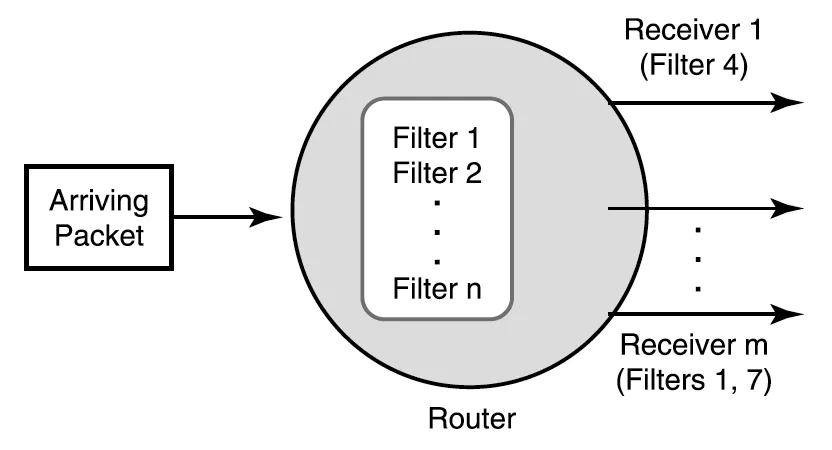
\includegraphics[width=0.8\textwidth]{../assets/ch01/ch01-1_2_网络算法学-016.png}
\end{figure}
图4.16的左侧框架中，流量在T之前的瞬间发送一个大小为B的突发，并在T之后的瞬间发送第二
个大小为B的突发，从而在一个略大于T/2的时间段内发送2B。




The naive use of a single or multiple timers (to check whether a flow sends no more than B every
T seconds) does not catch all violations.
不幸的是，两个计时器都无法检测到流量作为违规者。这种流量可以通过在每个被监管的时间段内发送
不超过B比特的数据来避免被检测为违规者，但在某些重叠的时间段内可能会发送超过B比特的数据。
为了解决这个问题，可以尝试使用多个计时器和计数器。例如，路由器可以使用一个从0开始的计时器和
另一个从T/2开始的计时器。然而，流量仍然可以通过在每个被监管的时间段内发送不超过B比特的数据
来规避检测，同时在某些重叠的时间段内发送超过B比特的数据。例如，在图4.16的右侧框架中，违规流
量在第一个时间段的末尾发送一个大小为B的突发，然后在第三个时间段的开始发送第二个大小为B的突
发，从而在一个略大于T/2的时间段内发送了2B。然而，这两个计时器都无法检测到该流量作为违规
者。
因此，需要一种更有效的方法来检测违规流量。可以考虑利用一些自由度（P13），这些自由度在简单解
决方案中被假定为固定的。是否需要固定监管间隔的开始时间？此外，考虑使用P3a。

                                                                                              42
解决方案
如提示所建议的，监管间隔不需要固定。因此，可以在计时器滴答之间设置任意的时间间隔。应该如何
选择这个间隔呢？由于违规流量可以选择在任何时刻开始其违规时间段T，一个简单的想法是引入以下概
念：
路由器使用一个T单位的计时器和一个计数器，如前所述。当计时器滴答时，如果计数器大于B，则检测
到违规行为。然后设置一个标志，指示计时器现在仅用于插入一个随机间隔。然后，计时器重新启动，
随机时间间隔在0到T之间。当计时器滴答时，清除标志并初始化计数器，并将计时器重置为T单位的时间
以开始下一次监管。
通过这种方式，违规流量无法预测监管间隔的开始时间，从而增加了被检测到的概率。
练习
● 假设计数器在间隔期间也被初始化和维护，即使在监管间隔之外的间隙期间也是如此。路由器能否
  在间隙期间做出任何有效的推断，即使间隙期间小于T单位？
● （开放问题）假设流量是有对抗性的。流量如何制定一个策略，以尽可能高地违反合同并仍然逃避
  前面描述的随机检测器的检测？流量策略可以是随机的。一个好的答案应该通过概率分析来支持。
4.10 识别资源消耗大户
假设一个设备希望跟踪各种用户的资源消耗情况，例如路由器分配给各个源的数据包内存。该设备需要
一种廉价的方法来找到消耗最多资源的用户，以便可以从这样的资源消耗大户那里回收内存。\begin{figure}[htbp]
\centering
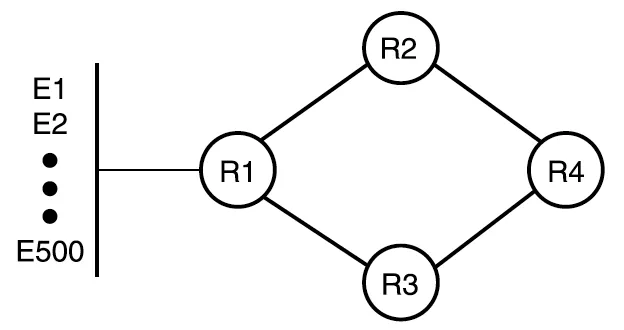
\includegraphics[width=0.8\textwidth]{../assets/ch01/ch01-1_2_网络算法学-018.png}
\end{figure}
图4.18显示
了五个源及其当前的资源消耗量分别为1、9、30、24和7个单位。资源消耗大户是S3。
问题
一个简单的解决方案是使用堆。然而，如果源的数量超过一千，这在高速情况下可能代价过高。假设描
述资源使用的数字是1到8000之间的整数。因此，桶排序技术可能不太适用，因为我们可能需要搜索
8000个条目才能找到资源消耗大户。
假设设备不关心确切的最大值，只要结果在2倍以内即可（P3b中提到的完美公平性不重要）。例如，在
图中，假设得到24而不是30是可以接受的。这种对准确性要求的放宽能否转化为更高效的算法？
提示：考虑使用三个原则：通过交易准确性来减少计算量（P3b）、使用桶排序（P14）和使用表查找
（P4b，P2a）。
解决方案
                                              43
由于结果可以在2倍以内，将资源消耗在2倍以内的用户聚合到同一个“资源消耗组”是有意义的。如果结
果组的数量比原始用户数量小得多，那么找到最大组将比找到最大用户更快。这类似于分层路由中的聚
合概念，其中多个目的地被聚合在一个共同的前缀下；这可能会使路由不够精确，但减少了路由条目的
数量。这导致了以下思路（在继续阅读之前尝试自己理清细节）。
可以使用二项式桶排序，如\begin{figure}[htbp]
\centering
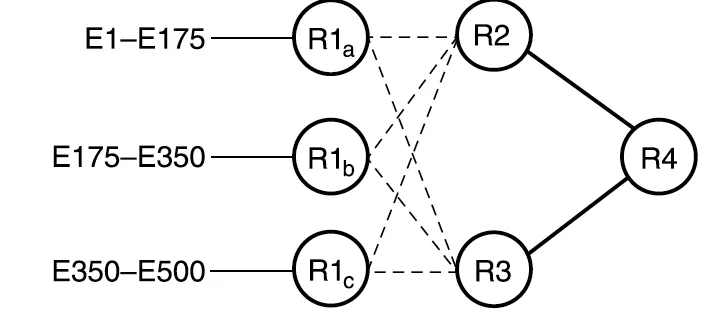
\includegraphics[width=0.8\textwidth]{../assets/ch01/ch01-1_2_网络算法学-019.png}
\end{figure}
图4.19所示，所有用户根据资源消耗被分组到不同的桶中，其中桶i包含所有
资源消耗在 2i 到 2i+1 − 1 之间的用户。例如，在图4.19中，用户S3和S4都在[16, 31]范围内，因此他
们在同一个桶中。
每个桶包含一个未排序的用户资源记录列表，这些记录落在该桶的范围内。因此，在图4.19中，S3和S4
在同一个列表中。该数据结构还包含一个位图，每个桶对应一个位，如果相应的桶列表非空，则设置该
位（图4.19）。因此，在图4.19中，对应于桶[1,1]、[4,7]、[8,15]和[16,31]的位被设置，而对应于[2,3]的
位被清除。
练习
 ● 这种数据结构是如何维护的？如果某个用户的资源（例如S3）从30减少到16，会发生什么？需要什
   么样的列表来进行有效的维护？
 ● 每个位图有多大？如何高效地找到最右边的设置位？



4.11 消除TCP连接列表
像TCP这样的传输协议在计算机X中为X与其他计算机之间的每个并发会话保持状态。回想一下第2章中提
到的，两个端点之间共享的状态的技术名称是连接。因此，如果用户希望从X向另一台工作站Y发送邮
件，X中的邮件程序必须首先建立与Y中的邮件程序的连接（共享状态）。像Web服务器这样的繁忙服务
器可能有许多并发连接。
连接的状态包括X发送的未被Y确认的数据包数量等信息。任何长时间未被确认的数据包都必须由X重新
传输。为了进行重新传输，传输协议通常有一个周期性计时器来触发重新传输那些长时间未被确认的数
据包。
自由的BSD TCP代码（Stevens，1994年）维护了一个连接列表（\begin{figure}[htbp]
\centering
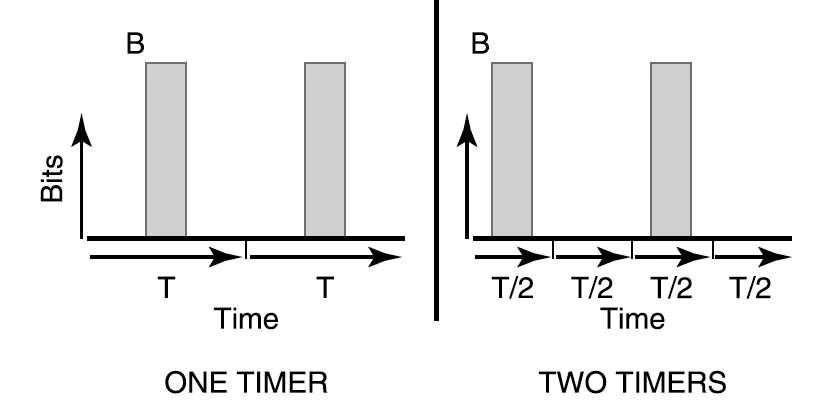
\includegraphics[width=0.8\textwidth]{../assets/ch01/ch01-1_2_网络算法学-020.png}
\end{figure}
图4.20），以便在计时器滴答时检查
是否需要重新传输。然而，当数据包到达X时，TCP还必须快速确定该数据包属于哪个连接，以便更新连
接的状态。每个连接由数据包中携带的连接标识符标识。
依赖于列表来确定数据包的连接在最坏情况下需要搜索整个列表；对于具有大量连接的服务器来说，这
可能很慢。因此，x-kernel实现（Hutchinson和Peterson，1991年）在BSD实现中添加了一个哈希表
（P15），以高效地将数据包中的连接标识符映射到相应的连接状态。哈希表是一个数组，索引由哈希值
指向存储相同哈希值的连接列表。此外，保留了原始的连接列表用于计时器处理，而哈希表用于加速数
据包处理。
                                                                44
然而，对新实现的测量实际上显示了速度变慢！仔细的测量表明，问题在于信息冗余存储，这降低了现
代处理器上数据缓存的效率（参见第2章中的现代处理器模型）。这说明了第3章中的问题Q3，即对系统
的一个部分的明显改进可能会影响系统的其他部分。虽然主内存可能很便宜，但快速内存如数据缓存通
常是有限的。常用的结构如连接列表应尽可能小，以便能够放入数据缓存。
显而易见的解决方案是避免冗余。哈希表用于快速查找。计时器例程还必须定期高效地扫描所有连接。
这导致了以下问题。
问题
能否在保留哈希表的同时消除显式连接列表造成的浪费？可以添加少量额外信息到哈希表。当这样做
时，注意到原始连接列表是双链的，以便在连接终止时轻松删除。然而，这增加了存储并降低了数据缓
存的效率。如何在不使用双链表的情况下使用单链表？
提示：第一部分可以通过将有效的哈希表条目链接在一个列表中来轻松解决。第二部分（避免双链表，
这需要在每个哈希表条目中使用两个指针）稍微困难一些。
连接列表由节点组成，每个节点包含一个连接ID（IP的96位）加上两个指针（假设各32位）以便于删
除。由于哈希表用于快速解复用，如果有效哈希表条目被链接在一起，如\begin{figure}[htbp]
\centering
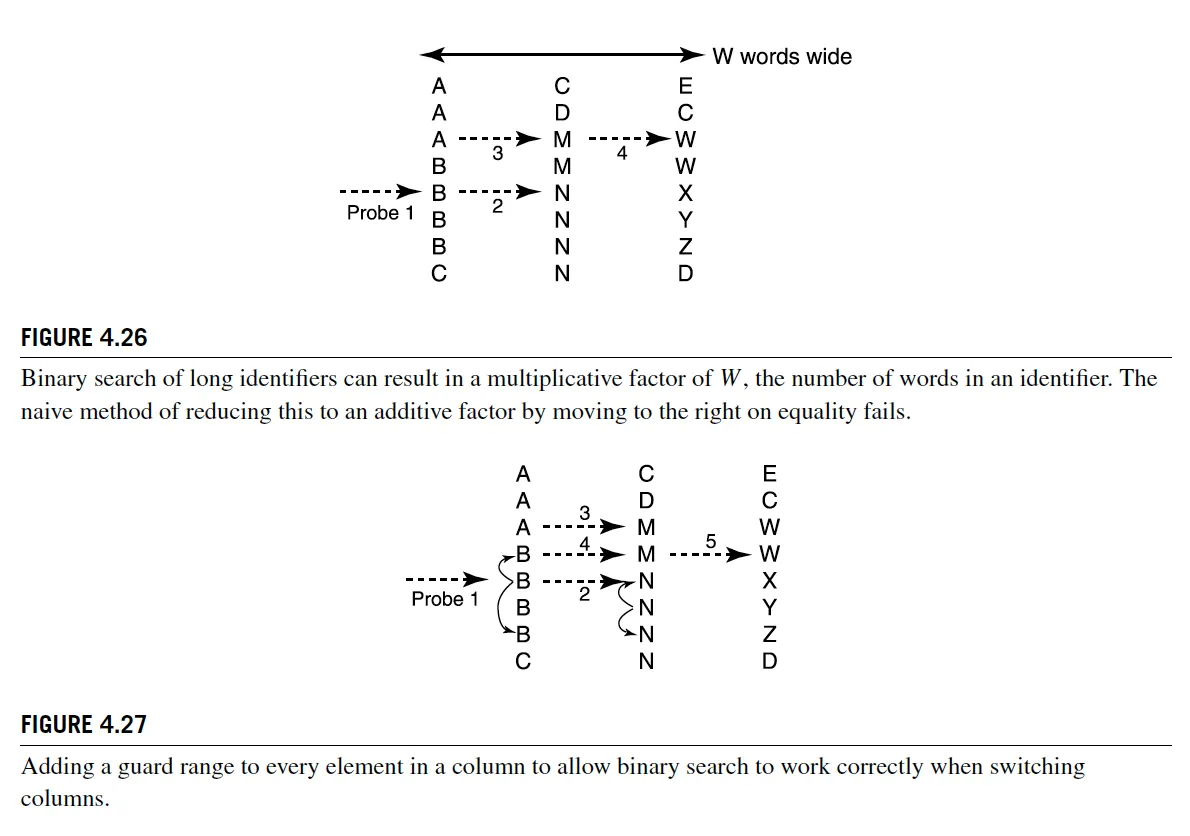
\includegraphics[width=0.8\textwidth]{../assets/ch01/ch01-1_2_网络算法学-021.png}
\end{figure}
图4.21所示，并且保持一个指向
列表头部的指针，则可以移除连接列表。在计时器滴答时，重传例程将定期扫描此列表。完整扫描哈希
表效率较低，因为哈希表可能有许多空位置。
解决方案
双链表仅对高效删除有用。当连接（例如图4.21中的连接C3）终止时，删除例程理想情况下希望找到前
一个有效条目（即图4.21中的包含连接C1的列表），以便将前一个列表链接到下一个列表（即包含C2的
列表）。这需要每个哈希表条目存储一个指向前一个有效条目的指针。
相反，考虑原则P3，该原则询问系统要求是否可以放宽。通常，假设当连接终止时，其存储必须立即回
收。为了回收存储，哈希表条目应放置在空闲列表中，以便可以被另一个连接重用。然而，如果哈希表
比严格需要的稍大，则不必立即重用终止连接的存储。
鉴于这种放宽要求，实现可以延迟删除连接状态。当连接终止时，必须将条目标记为未使用。这需要一
个额外的位状态（如P12），但成本较低。实际删除未使用的哈希表条目E涉及将条目E之前的条目链接
到E之后的条目，并将E返回到空闲列表。然而，这种删除可以在下一次列表遍历时进行，当遍历遇到未
使用的条目时。
练习
●   编写伪代码以添加新连接、终止连接和基于计时器的遍历。

                                                45
● 如何仅使用单链表来实现每个哈希表列表中的连接列表？
● Hugh Hopeful总是对那些他从未彻底思考过的巧妙技巧感兴趣。他建议一种避免在双链表中使用反
  向指针的方法。通常，节点X需要被删除时，删除例程会传递一个句柄来检索X，这通常是一个指向
  节点X的指针。相反，Hugh建议句柄可以是指向链表中X之前节点的指针（除了X是链表头部时句柄
  为空指针）。Hugh声称这允许他的实现在仅使用前向指针的情况下高效地定位X之前和之后的节
  点。提出一个反例来阻止Hugh在编写有缺陷的代码之前继续。
4.12 确认抑制
像TCP这样的传输协议通过要求目的地对每条接收到的数据发送确认（ack）来确保数据被交付给目的
地。这类似于挂号信。数据包和确认都带有编号。确认通常是累积的；对编号为N的数据包的确认隐含地
确认了所有编号小于或等于N的数据包。
累积确认允许接收方灵活地不必为每条接收到的数据包发送确认。相反，确认可以批量处理（P2c）。例
如，在\begin{figure}[htbp]
\centering
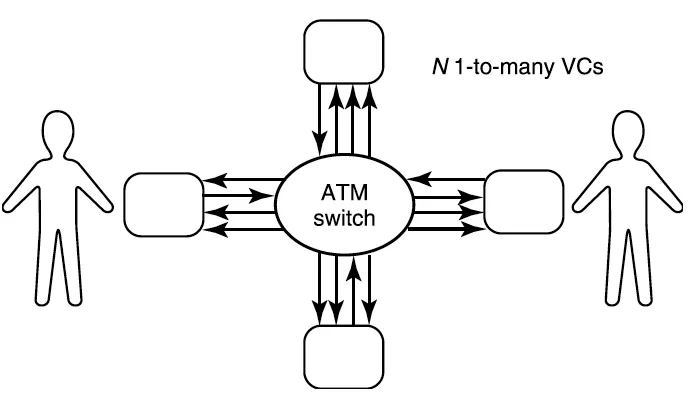
\includegraphics[width=0.8\textwidth]{../assets/ch01/ch01-1_2_网络算法学-022.png}
\end{figure}
图4.22中，文件传输程序正在发送文件块，每个数据包一个块。块1和2分别被确认，但块3和4通
过一个确认块4来确认。
减少确认的数量对发送方和接收方都有好处。尽管确认很小，但它们包含必须由每个路由器和源及目的
地处理的头部。此外，每个接收到的数据包，无论多小，都可能在目的地计算机上引起中断，而中断是
昂贵的。因此，理想情况下，接收方应尽可能批量确认。但是，接收方应该如何制定确认抑制策略以避
免不必要的延迟，同时又能有效地批量确认？
问题
在接收方不是先知的情况下，确认抑制是困难的。例如，在图4.22中，如果块3首先到达并被快速处理，
接收方应该等待块4多久才发送块3的确认？如果块4永远不会到达（因为发送方没有更多数据要发送），
那么抑制块3的确认将导致错误行为。经典的解决方案是设置一个确认抑制计时器；当计时器到期时，发
送累积确认。这限制了确认可以被抑制的时间。
然而，抑制计时器也会导致问题。某些应用程序对延迟敏感。添加确认抑制计时器可能会增加延迟，特
别是在发送方没有更多数据要发送的情况下。如果传输协议可以修改，可以添加什么信息来避免不必要
的延迟，同时又能有效地批量确认？
提示：在像FTP这样的应用程序中，哪个软件模块知道还有更多数据要发送？对于确认抑制，哪个软件模
块理想情况下希望知道还有更多数据要发送？现在考虑使用P9和P10。
解决方案

                                                  46
在像文件传输这样的应用程序中，发送方应用程序知道还有更多数据要发送（例如，将有块4在块3之
后）。发送方应用程序也可能愿意容忍由于确认批量处理而导致的延迟。然而，需要知道此信息的接收
方传输模块。这引出了一个简单的提议。
发送方应用程序向发送方传输层传递一个位（在应用程序-传输接口中），当应用程序有更多数据要发送
时，该位被设置。假设传输协议可以修改以携带一个抑制位。发送方传输层可以使用应用程序传递的信
息来设置每个数据包中的抑制位w；当发送方希望立即确认时，清除该位。关键是发送方传达其意图比接
收方猜测未来更好！
例如，在\begin{figure}[htbp]
\centering
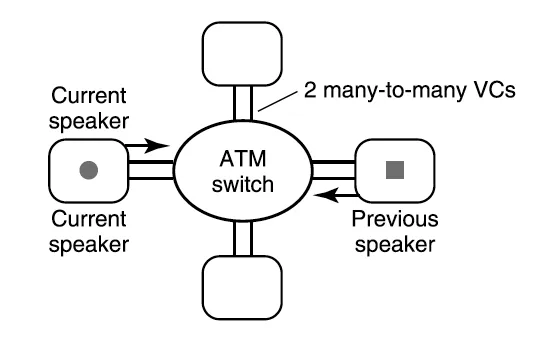
\includegraphics[width=0.8\textwidth]{../assets/ch01/ch01-1_2_网络算法学-023.png}
\end{figure}
图4.23中，发送方传输层被告知发送文件传输应用程序有四个块要发送。因此，发送方传输层
在前三个数据包上设置抑制位，并在第四个数据包上清除该位。接收方根据此信息发送一个确认而不是
四个。另一方面，对延迟敏感的应用程序可以选择不传递有关要发送数据的任何信息。还要注意，抑制
位是一个提示；接收方可以选择忽略此信息并仍然发送确认。尽管这个解决方案看起来很巧妙，但在今
天的TCP中却是一个糟糕的主意。请参阅练习了解更多细节。
练习
● 另一种减少确认的方法是将确认信息附加到从接收方到发送方的数据流中。为了支持这一点，大多
  数传输协议（如TCP）在数据包中有额外的字段来传达反向确认信息。然而，附加确认存在延迟和
  附加确认效率之间的权衡。接收方传输层应该等待多长时间以获取反向数据？另一方面，有许多常
  见应用程序，其中发送方应用程序知道这些信息。如何扩展前面概述的解决方案以支持附加确认以
  及确认批量处理？
● 回想一下第3章中概述的一组用于评估所谓改进的警示问题。例如，问题Q3询问更改是否会影响系
  统的其他部分。为什么激进的确认抑制可能与传输协议的其他方面（如流量控制和拥塞控制
  （Stevens，1994年））相互作用？
4.13 增量读取大型数据库
假设用户连续读取存储在网站上的大型数据库。网页可能会更改，读者只希望获取自上次读取数据库以
来的增量更新（P12a）。因此，在图4.24中，有一个包含广受欢迎食品项目的数据库，全球读者不断阅
读以跟上美食潮流。幸运的是，美食潮流变化缓慢。
因此，一个在下午2点阅读并在下午6点再次阅读的读者只希望获取差异：可口可乐到百事可乐，以及麦
片到 Cheerios。另一方面，如果另一个读者在下午3点阅读并在下午6点阅读，她也只希望获取差异：麦
片到 Cheerios。这导致了以下问题。
问题

                                                  47
找到一种方法，使数据库能够高效地执行此类增量查询。一种解决方案是让数据库记住每个用户上次读
取的内容。然而，要求数据库记住每个用户上次读取的内容是不合理的，因为可能有数百万用户。找到
一种对数据库程序负担较小的解决方案。
提示：如果数据库不存储有关用户上次读取的任何信息，那么用户读取请求必须传递一些信息（P10）关
于同一用户的最后一次读取请求。传递整个上次读取的详细信息将是过度的且低效的。用户上次请求的
最简洁和相关的信息是什么？现在考虑在数据库中添加冗余状态（P12），以便可以使用用户传递的信息
高效地处理增量查询。
解决方案
如前所述，用户读取请求必须传递一些信息（P10）关于同一用户的最后一次读取请求。关于最后一次用
户请求的最简洁和相关的信息是它被执行的时间。如果用户请求传递上次读取的时间T，则数据库需要以
一种高效计算自时间T以来的所有更新的方式来组织。这可以通过存储数据库在所有可能先前时间的副本
来实现。这显然是低效的，可以通过仅存储增量更改（P12a）来避免。这导致了以下算法。
向数据库添加一个更新历史列表，用户读取请求传递上次读取的时间T，因此可以通过扫描更新列表从头
部开始查找自时间T以来的所有更新来处理读取请求。
例如，在图4.25中，更新历史列表的头部是最新的更改（比较图4.24），在下午6点从麦片到
Cheerios，下一个最早的更改是在下午3点从可口可乐到百事可乐。考虑一个读取请求，其上次读取时间
为下午5点。在这种情况下，扫描列表从头部开始，找到下午6点的更新并停止，因为3<5。因此，读取
请求将只返回第一个更新。
练习
● 如果单个条目多次更改，单个条目更改可以在列表中冗余存储，这会消耗空间和时间。可以使用什
  么原则来避免这种冗余？假设数据库只是记录的集合，并且希望每个记录在增量列表中最多出现一
  次。
● 如果记录数量很大或未采用前述技巧，则增量列表的大小将变得非常大。建议一个合理的策略定期
  减少增量列表的大小。
4.14 长标识符的二分搜索
下一代互联网（IPv6）计划使用更大的128位地址以适应更多终端。假设需要对128位地址进行查找，且
算法运行在自然字长为32位的机器上。那么比较两个128位数字需要4次操作（每个字单独比较）。一般
而言，若每个标识符由W个字组成（本例中W=4），朴素的二分搜索需要W·logN次比较，代价高昂。


                                                 48
显然这种方法存在浪费。如果所有标识符的前W-1个字都相同，那么仅需logN次比较即可。问题在于如
何改进二分搜索，使其仅需logN + W次比较。策略是按列处理：从最高有效字开始，在该列进行二分搜
索直至找到匹配项，然后右移到下一列继续搜索。
如图4.26所示（设W=3），假设搜索三字标识符"BMW"（每个字符视为一个字）。首先在左列中间元素
进行比较（图中标为1的箭头）。当搜索字符串的"B"与该位置匹配时，搜索右移到第二列中间位置比
较"M"和"N"。由于N < M，搜索转向第二列的四分之一位置。此时两个"M"匹配，搜索继续右移找
到"W"——但错误地找到了"AMW"而非目标"BMW"。




问题
如何为每列的每个元素添加状态，使得算法能在logN + W次比较内正确工作？
提示：问题根源在于搜索移到第二列四分之一位置时，假设该区域所有元素的左列都以"B"开头。如何通
过添加状态避免这种错误假设？如何修改搜索逻辑来利用这种状态？
解决方案
关键是为每列元素添加守卫范围（guard range）状态。如图4.27所示，对于左列字符（如"B"），添加
指向所有左列同为"B"的元素的指针范围。搜索"BMW"时，首先比较左列"B"（位于"BNX"处）。匹配后
搜索移到第二列，同时记录左列"B"对应的守卫范围（图中第4-7行）。
当发现"M" < "N"时，尝试将搜索范围折半到第三项（"AMW"的"M"）。但该位置低于当前守卫范围下限
（第4行），因此不进行比较直接再次折半到第4项。在此匹配后右移，最终正确找到"BMW"。
                                                     49
通用规则：每个多字条目W1,W2,...,Wn都预计算守卫范围。Wi的范围指向前i个字为W1...Wi的所有条目。
该方案仅需log2N + W次探测，代价是每个字增加两个16位指针（共32位）。由于机器字长通常≥32
位，内存占用最多翻倍。该方案由Butler Lampson提出，核心思想是通过预计算（P2a）换取搜索效
率。


4.15 基于ATM的视频会议系统
图4.28展示了一个ATM交换机连接N个工作站的拓扑。为展示交换机带宽，系统设计者开发了视频会议
应用：任意工作站用户可发起会议，每个参会者屏幕需至少显示当前发言者并播放其语音。多人对话时
还需观察参与者表情。




A videoconferencing system that uses an ATM switch with the ability to support many-to-many
VCs.
问题
最朴素方案需N²个点对点连接，较好方案（图4.28）采用N个一对多VC（虚拟通道），每个工作站视频
流通过独立VC广播给其他参会者。但ATM交换机需静态分配带宽，设单路视频最小带宽Bmin，交换机
总带宽B，则最大参会人数受限于B/Bmin。是否存在更可扩展的方案？
提示：考虑利用交换机硬件支持多对多VC的特性（P4c）。为确保单一发言，可添加硬件（P5）而非复
杂协议。如何通过硬件设计避免多源同时传输？




                                                                                              50
Replacing N one-to-many VCs with two many-to-many VCs through the use of a speech
detector and a simple hardware state machine at each input.
解决方案
如提示所述，设计者选择利用交换机的多对多VC能力，用恒定数量的多对多VC替代N个一对多VC。这使
得固定交换机带宽能够扩展到大量参与者。然而，这一通用思路需要进一步细化：应该使用多少个多对
多VC？如何解决多对多VC可能导致的混乱问题？以下是华盛顿大学Jon Turner提出的具体解决方案细
节。
首先，考虑使用单个多对多VC（命名为C）。解决混乱问题的简单方案是通过协议（例如轮询协议）确
保每次只有一个工作站将其视频输出连接到C。这类协议需要协调，而协调会增加延迟和成本。作为系统
思考者，设计者观察到，至少需要显示当前发言者。因此，设计者在每个工作站的输入端额外添加了语
音检测硬件（P5）。如果检测器在工作站X检测到显著语音活动，则将X的视频输入连接到C；否则，X
的视频输入不与C连接。由于这类硬件成本低廉，扩展性提升的代价非常合理。
接下来，设计者注意到，在典型的双人对话场景中，保留最后一位发言者的视频图像能提供视觉连续
性。因此，他们不再使用单个多对多VC，而是采用两个多对多VC（C和L），分别对应当前发言者和最
后一位发言者，如图4.29所示。




                                                                                    51


\chapter{端系统：定时器}
% 来源: 19c9fbd0-f1d2-808a-8000-0000b4a1e732_1.5_端_定时器.pdf
% 提取时间: 2026-02-28T22:51:53+08:00

1.5 端：定时器
第7章 定时器维护
“过去如是，现在如是，将来亦如是：时光之轮永不停歇。”——罗伯特·勃朗宁
系统中的定时器模块就好比是一位秘书，负责记录忙碌主管的所有日程安排。主管告知秘书安排日程，
有时还会要求在日程开始前取消安排。秘书的工作是在日程即将开始前提醒主管。实际上，许多秘书会
使用所谓的“到期提醒文件”来完成这项工作，这是一个涵盖未来N天的动态窗口。当一天的日程结束后，
到期提醒文件会滚动更新，跳过当天。我们会发现到期提醒文件和本章的主要数据结构——时间轮有很
强的相似性。
本章内容安排如下：7.1节描述了为什么需要定时器；7.2节介绍了定时器例程的模型以及对性能至关重要
的相关参数；7.3节讲述了维护定时器的最简单技术，其中一些在某些情况下仍然适用；7.4节引入了主要
数据结构——时间轮，随后在7.5节和7.6节分别介绍了时间轮的两种具体实例：哈希轮和分层时间轮；本
章最后在7.9节介绍了一种称为软定时器的技术，它通过在其他系统调用中分摊定时器维护开销来降低定
时器的开销。表7.1总结了各种定时器方案中应用的原理。
与第一版相比，最显著的变化可能是如今云主机中经常使用成千上万的细粒度定时器（Saeed等人，
2017）。这些定时器通过流量整形为虚拟机流量提供带宽隔离，并且用于像BBR（Cardwell等人，
2017）这样的现代拥塞控制算法中，BBR算法通过精细的速率调整来减少数据包丢失。这些新应用更有
力地证明了使用本章主要数据结构（时间轮）的必要性，以及在多核机器中实现更精简定时器的需求。
快速参考指南
对于实现者而言，最有用的部分可能是7.5节关于哈希时间轮的内容。哈希时间轮的多个版本已出现在许
多操作系统中，例如FreeBSD，以及在谷歌机器中作为Carousel（Saeed等人，2017）流量整形软件的
一部分。Linux早期版本以及最近一个版本使用分层时间轮（7.6节），这个版本效率更高，但定时器精
度较低（Corbet，2015）。
 序号                原理                   定时器技术
 P14               使用数组存储有界定时器          基本时间轮
 P2c, 4            利用每日时间更新             /
 P15               使用哈希或分层结构            哈希、分层时间轮
 P10               传递句柄以删除定时器           任何定时器方案
 P4                利用系统调用等              软定时器

                                                       1
P3                 放宽对精确定时器的需求       /
P11                优化快速定时器           /

7.1 为什么需要定时器？
系统为什么需要定时器呢？系统需要定时器来进行故障恢复，同时也用于实现一些算法，在这些算法
中，时间或相对时间的概念是不可或缺的。有几种类型的故障无法异步检测到。有些故障可以通过定期
检查来发现（例如，磁盘看门狗定时器），这类定时器总是会到期。而其他一些故障只能通过在指定时
间内没有某些积极动作（例如，消息确认）来推断。如果故障很少发生，这些定时器很少会到期。
许多系统还会实现使用时间或相对时间的算法。例如，控制某些实体产生速率的算法（如网络中的基于
速率的流量控制）和调度算法。这些定时器几乎总是会到期。
当出现以下任何一种情况时，实现定时器模块的算法性能就会成为一个问题。首先，如果该算法由一个
处理器实现，并且每次硬件时钟滴答时处理器都会被中断，且中断开销很大，那么性能就会成为问题。
其次，如果需要细粒度的定时器，性能也会成为问题。第三，如果活动定时器的平均数量很大，性能同
样会成为问题。在运行速度为100 Gbps、对成千上万的流量进行精细流量整形的云服务器中，这三个因
素正变得越来越关键（Saeed等人，2017）。
如果硬件时钟每次滴答都中断主机，且滴答之间的间隔在微秒量级，那么中断开销是相当大的。大多数
主机操作系统提供的定时器粒度较粗（毫秒或秒）。或者，在某些系统中，更细粒度的定时器存在于专
用硬件中。在这两种情况下，定时器算法的性能都会是一个问题，因为它们决定了启动或停止定时器所
产生的延迟以及可以同时存在的定时器数量。
例如，考虑分布式系统中成员之间的通信。由于消息可能在底层网络中丢失，因此在某种程度上需要定
时器来触发重传。分布式系统中的一个主机可能有多个未完成的定时器。例如，一台有50,000个连接的
服务器，每个连接有三个定时器。此外，随着网络速度提升到100吉比特及更高，所需的定时器分辨率以
及启动和停止定时器的频率都会增加。
一些网络实现并不是为每个数据包都使用一个定时器，而是整个网络包只使用几个定时器。例如，TCP
实现通过为所有未完成的数据包维护自己的定时器，并使用单个内核定时器作为时钟来运行这些定时
器，从而仅用两个定时器就解决了问题。TCP以最简单的方式维护其数据包定时器：每当其单个内核定
时器到期时，它就会对所有未完成的数据包定时器进行计数。例如，许多TCP实现使用两个定时器：一
个200毫秒的定时器和一个500毫秒的定时器。
如果定时器的粒度较低且丢失情况很少发生，这种简单的方法效果还不错。然而，提高重传定时器的分
辨率以实现更快的恢复是很有必要的。例如，亚利桑那大学有一种名为TCP Vegas（Brakmo等人，
1994）的TCP实现，其性能优于常用的TCP Reno。TCP Reno在遇到丢失情况时性能较差的原因之一就
是超时的粒度较粗。

                                                      2
除了更快的错误恢复，细粒度定时器还能让网络协议更精确地测量更短的时间间隔。例如，准确估计往
返延迟对于TCP拥塞控制算法（Jacobson，1988）和在网络会议工具（McCanne，1992）中实现的
SRM（可扩展可靠多播）框架（Floyd等人，1995）非常重要。
最近，除了准确的往返延迟测量，现代拥塞算法也开始使用细粒度定时器。例如，谷歌的BBR算法
（Cardwell等人，2017）使用精细的速率调整来减少网络中的数据包丢失，特别是对于视频流。
最后，许多多媒体应用程序经常使用定时器，而且这类应用程序的数量还在不断增加。早期的一个例子
是西门子用于多媒体的CHANNELS运行时系统（Boecking等人，1995），其中每个音频流使用的定时
器粒度在10到20毫秒之间。对于多媒体和其他实时应用程序来说，确定启动和停止定时器的最坏情况处
理时间上限非常重要。
除了网络应用，过程控制和其他实时应用也将从大量细粒度定时器中受益。此外，系统上的用户数量可
能会增长到足够多，从而导致大量未完成的定时器。这就是IBM VM/XA SP1操作系统开发者重新设计定
时器功能的原因（Davison，1989）。
在接下来的章节中，我们将描述一系列基于一种称为时间轮的数据结构来高效实现定时器的方案。我们
还将介绍一些基于本章思想实现定时器包的系统。
7.2 模型和性能指标
定时器模块（Varghese和Lauck，1987）有四个组件例程：
 ● STARTTIMER(Interval, RequestId, ExpiryAction)：客户端调用这个例程来启动一个定时器，该定
   时器将在“Interval”个时间单位后到期。客户端提供一个RequestId，用于区分这个定时器与客户端
   其他未完成的定时器。最后，客户端可以指定定时器到期时要执行的操作，例如，调用客户端指定
   的例程或设置一个事件标志。
 ● STOPTIMER(RequestId)：这个例程利用它对客户端和RequestId的了解来定位定时器并停止它。
 ● PERTICKBOOKKEEPING：假设定时器的粒度为T个时间单位。那么每隔T个时间单位，这个例程会
   检查是否有未完成的定时器到期；如果有，它会调用STOPTIMER，而STOPTIMER又会调用下一个
   例程。
 ● EXPIRYPROCESSING：这个例程执行STARTTIMER调用中指定的ExpiryAction操作。

前两个例程在客户端调用时被激活；后两个例程在定时器滴答时被调用。定时器通常是一个外部硬件时
钟。
可以使用两个性能指标来选择本章其余部分描述的算法。这两个指标都由n参数化，n表示未完成定时器
的平均（或最坏情况）数量。它们分别是定时器数据结构所需的空间（Space）和延迟（Latency），即
定时器模块中一个例程被调用到完成之间的时间。假设例程的调用者会阻塞，直到例程完成。平均延迟
和最坏情况延迟都值得关注。

                                                                    3
7.3 最简单的定时器方案
实际上，两种最简单的定时器实现方案被广泛使用。在第一种方案中，STARTTIMER找到一个内存位
置，并将该位置设置为指定的定时器间隔。每隔T个时间单位，PERTICKBOOKKEEPING会递减每个未
完成的定时器；如果某个定时器的值变为零，则调用EXPIRYPROCESSING。
除了PERTICKBOOKKEEPING操作外，这个方案对于其他操作来说都非常快。它为每个未完成的定时器
使用一个记录，这是可能的最小空间占用。如果未完成的定时器数量很少，大多数定时器在时钟的几个
滴答内就被停止，并且PERTICKBOOKKEEPING由专用硬件以合适的性能完成，那么这个方案是合适
的。
请注意，我们可以存储定时器到期的绝对时间并进行比较，而不是进行递减操作。这个选项适用于我们
描述的所有定时器方案；在它们之间的选择将取决于时间字段的大小、每条指令的成本以及实现这些算
法的机器硬件。在本章中，除了描述方案2时，我们将使用递减选项。
                          10:23:12




                          10:23:24




                          10:24:03


\begin{figure}[htbp]
\centering
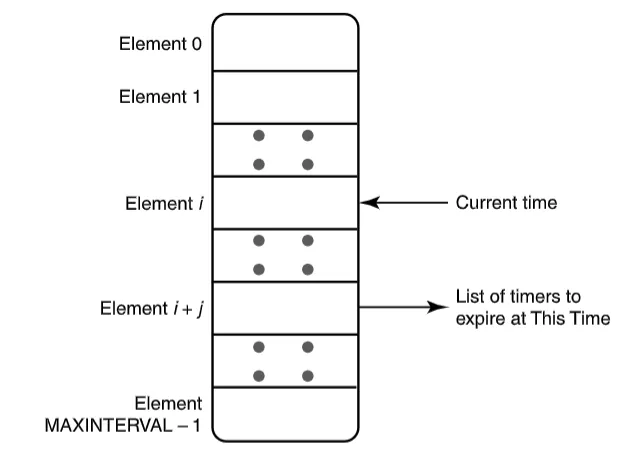
\includegraphics[width=0.8\textwidth]{../assets/ch01/ch01-1_5_端_定时器-001.png}
\end{figure}
图7.1用于说明方案2的定时器队列示例
在第二种简单方案中（用于UNIX的旧版本），PERTICKBOOKKEEPING的延迟降低了，但这是以
STARTTIMER的性能为代价的。定时器存储在一个有序列表中。与方案1不同，我们将存储定时器到期的
绝对时间，而不是到期前的间隔时间。最早到期的定时器存储在列表的头部。后续的定时器按递增顺序
存储，如图7.1所示。在图7.1中，最早到期的定时器将在绝对时间10小时23分12秒到期。



由于列表是排序的，PERTICKBOOKKEEPING只需要增加当前时钟时间，并将其与列表头部进行比较。
如果两者相等，或者当前时间大于列表头部的时间，它就会删除该列表元素，并调用
EXPIRYPROCESSING。它会继续删除列表头部的元素，直到列表头部的到期时间严格小于当前时间。
STARTTIMER通过搜索列表来找到插入新定时器的位置。在示例中，STARTTIMER将把一个在10:24:01
到期的新定时器插入到第二个和第三个元素之间。
                                                        4
启动定时器的最坏情况延迟是O(n)。平均延迟取决于定时器间隔（从开始时间到停止时间）的分布以及
调用STARTTIMER的到达过程的分布。
如果列表是双向链表，STOPTIMER就不需要搜索列表。当STARTTIMER将一个定时器插入到有序列表
中时，它可以存储一个指向该元素的指针。然后STOPTIMER可以使用这个指针在O(1)时间内从双向链表
中删除该元素。这可以应用于任何定时器方案。这是P9原则（在层接口中传递提示）的一个应用。更准
确地说，用户在STOPTIMER接口中向定时器传递一个句柄。
如果这个方案由主机处理器实现，并且有硬件支持来维护单个定时器，那么每次滴答时的中断开销就可
以避免。硬件定时器被设置为在列表头部的定时器到期时到期。硬件会拦截所有时钟滴答，只有当定时
器实际到期时才会中断主机。不幸的是，一些处理器架构不提供这种能力。
在空间方面，方案1需要尽可能少的空间；方案2需要O(n)的额外空间来存储队列元素之间的前向和后向
指针。
链表是实现优先级队列的一种方式。对于较大的n，基于树的数据结构更好。这些数据结构包括非平衡二
叉树、堆、后序和终序树以及左偏树（Cormen等人，1990；Vaucher和Duval，1975）。它们试图将方
案2中STARTTIMER的延迟从O(n)降低到O(log(n))。在Myhrhaug（2001）中报告称，对于较大的n，这
种差异是显著的，并且非平衡二叉树比平衡二叉树成本更低。
不幸的是，非平衡二叉树很容易退化为线性列表；例如，如果插入一组相等的定时器间隔，就会发生这
种情况。不过，将时间轮的性能与使用简单二叉堆的实现进行比较是个好主意。我们将这些算法归为方
案3：基于树的算法。Linux高分辨率定时器（hrtimers）使用平衡（红黑）树（Gleixner和Niehaus，
2006）。
因此，这三种简单方案在STARTTIMER或PERTICKBOOKKEEPING操作中，花费的时间至少与定时器数
量成对数关系。这对于高速实现来说是个问题。下一节将展示如何做得更好。
7.4 时间轮
第一种方案的设计遵循一种常见的问题解决范式：先解决一个更简单的问题，然后利用从中获得的见解
来解决更复杂的问题。
我们首先处理的更简单问题如下。假设所有定时器都设置为某个较小的间隔，例如MAXINTERVAL，并
且假设定时器的粒度为1个时间单位。这表明可以使用P4原则（桶排序技术），而不是方案2和方案3中建
议的排序技术。然而，桶排序实际上用于对一组数字进行静态排序。在这里，新的数字不断被添加和删
除，而我们仍然希望保持顺序。（从技术算法角度来说，定时器数据结构必须实现一个优先级队列，支
持添加、删除和查找最小元素的操作。）与优先级队列等价的桶排序是什么呢？
基于这个动机，不难让读者脑海中浮现出以下画面（如\begin{figure}[htbp]
\centering
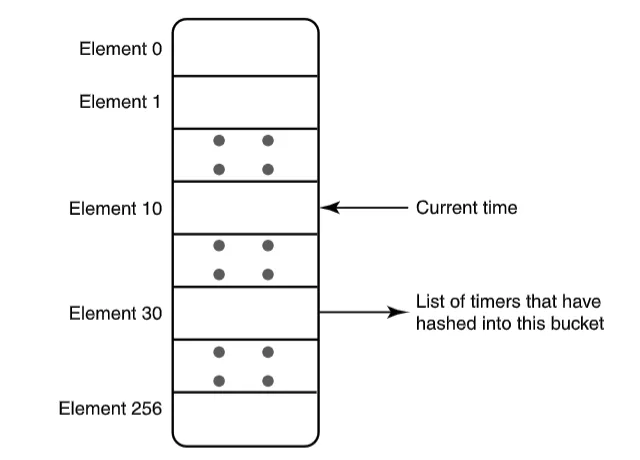
\includegraphics[width=0.8\textwidth]{../assets/ch01/ch01-1_5_端_定时器-002.png}
\end{figure}
图7.2所示）。想象当前时间由一个指向循环数组
中某个元素的指针表示，该循环数组的维度为[0, MAXINTERVAL - 1]。在每次定时器滴答（用于每滴答
记账）时，我们只需将指针增加1，并对数组大小取模。
                                                             5
图7.2方案4用于最大间隔为MAXINTERVAL的定时器的列表数组
要设置一个在当前时间之后j个时间单位到期的定时器，我们对元素(i + j) mod MAXINTERVAL进行索引
（见图7.2），并将定时器放在一个定时器列表的头部，该列表中的定时器将在时间 = 当前时间 + j个时
间单位时到期。每次滴答时，我们递增当前定时器指针（对MAXINTERVAL取模），并检查指针指向的
数组元素。如果该元素为0（没有等待到期的定时器列表），那么在该定时器滴答时就不再进行其他工
作。但是，如果该元素不为零，那么我们对存储在该列表中的所有定时器执行EXPIRYPROCESSING。
因此，STARTTIMER的延迟为O(1)；除了定时器到期时，PERTICKBOOKKEEPING的延迟也是O(1)，但
这已经是最好的情况了。如果定时器列表是双向链表，并且和之前一样，我们为每个定时器记录存储一
个指针，那么STOPTIMER的延迟也是O(1)。
我们可以更形象地将这个数组描述为一个时间轮，其中时间轮每个定时器单位转动一个数组元素。对于
秘书来说，这类似于到期提醒文件。对于排序专家来说，这类似于用空间换处理效率的桶排序。然而，
由于定时器的值随时都在变化，时间间隔是相对于当前时间指针的偏移量。只要当前时间指针随时递增
就足够了。
桶排序使用M个桶在O(M)时间内对N个元素进行排序，因为需要检查所有的桶。对于较大的M > N，这是
低效的。然而，在定时器算法中，关键的观察结果是，某个实体需要每滴答执行O(1)的工作来更新当前时
间；对于同一个实体来说，遍历一个空桶只需要多执行几条指令。这是使用P4原则（利用系统组件）和
P2c原则（费用分摊）的一个很好的例子。
系统已经在每滴答执行一些工作来增加时间。因此，在计算算法成本时，重要的是算法带来的额外开
销，而不是像在算法课上通常测量的那样单独计算成本。请注意，如果系统不是在每个时钟滴答都执行

                                                           6
一些工作，而是依赖于一块硬件来保持时间，那么这个假设就不成立。与排序不同，重要的不是对N个元
素进行排序的总工作量，而是每个定时器滴答需要执行的平均（和最坏情况）工作量。
然而，内存是有限的：很难为了实现32位定时器而分配2^32个字的内存。那么如何将这个想法扩展到更
大的定时器值呢？如果你之前没有接触过这个问题，在继续阅读之前，试着自己想出一些办法。
一种简单的解决方案是在给定的内存范围内使用这个方案来实现定时器。对于大于这个范围的定时器
值，可以使用其他方案，比如方案2。或者，这个方案可以通过两种方式进行扩展，以便在使用适量内存
的情况下支持更大的定时器间隔值。这两种技术的灵感来自两种算法技术（P15）：哈希和基数排序。
7.5 哈希轮
系统已经在每个时钟周期做了一些增加时间的工作。因此，在计算算法成本时，重要的是算法带来的额
外开销，而不是像在算法课上通常单独测量的成本。需要注意的是，如果系统不是在每个时钟周期都做
一些工作，而是依靠一块硬件来记录时间，那么这个假设就不成立。与排序不同，重要的不是对N个元素
进行排序的总工作量，而是每个定时器时钟周期需要完成的平均（以及最坏情况）工作量。
然而，内存是有限的：很难为了实现32位定时器而分配 232 个字的内存。那么，如何将这个想法扩展到
更大的定时器值呢？如果你之前没有接触过这个问题，在继续阅读之前，不妨先尝试自己思考一下解决
方案。
一种简单的解决方法是，在给定的内存和方案下，实现一定范围内的定时器。对于大于这个范围的定时
器值，可以采用其他方案，比如方案2。另外，这个方案可以通过两种方式进行扩展，以便在使用适量内
存的情况下支持更大的定时器间隔值。这两种技术的灵感来源于两种算法技术（P15）：哈希和基数排
序。
7.5 哈希轮
第一种扩展的设计遵循了第二种常见的问题解决范式：通过类比，从不同问题的解决方案中推导出解决
当前问题的技术。
许多想法最初都是通过类比产生的，尽管类比并不总是完全准确。前面的方案与使用元素值作为索引在
数组中插入元素有明显的相似之处。如果内存不足，我们可以对元素值进行哈希运算以得到一个索引
吗？例如，如果哈希表的大小是2的幂次方，那么任意大小的定时器值都可以很容易地除以哈希表大小；
余数（低阶位）与当前时间指针相加，得到数组中的索引。除法的结果（高阶位）则存储在由该索引指
向的列表中。
在\begin{figure}[htbp]
\centering
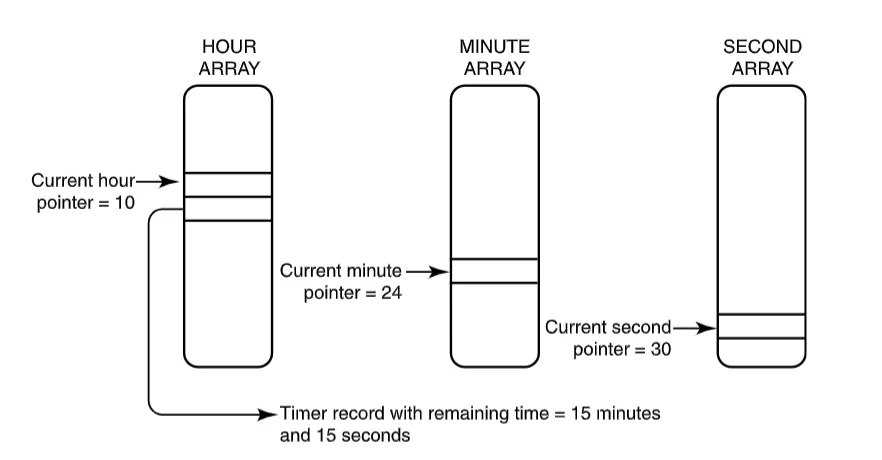
\includegraphics[width=0.8\textwidth]{../assets/ch01/ch01-1_5_端_定时器-003.png}
\end{figure}
图7.3中，假设哈希表大小为256，定时器为32位定时器。除法的余数是最后8位。假设最后8位的值为
20。那么定时器的索引就是10（当前时间指针） + 20（余数） = 30。然后，将24个高阶位插入到由第
30个元素指向的列表中。

                                                    7
也可以使用其他哈希方法。例如，可以使用任何将定时器值映射到数组索引的函数。我们将在7.5节末尾
阐述选择这种方法的理由。然而，现在我们的设计面临一个分歧点。无论使用哪种哈希函数，都有两种
维护每个列表的方式。
最直接的方法（在深入研究之前，这似乎是最好的方法）是在每个桶内采用方案2。这显然是对方案2的
扩展，同时提高了其性能，因为每个 “小” 列表应该比单个列表小。现在来详细说明一下。不幸的是，它
的性能取决于哈希函数，因为STARTTIMER操作可能会很慢，原因是24位的数量必须插入到列表中的正
确位置。因此，STARTTIMER的最坏情况延迟仍然是 O(n) 。
假设 O(n) 的STARTTIMER最坏情况延迟是不可接受的，我们可以将每个时间列表维护为无序列表，而
不是有序列表。乍一看，这似乎是个糟糕的主意。我们确实使STARTTIMER操作更快了；但是，如果列
表是无序的，那么每个时钟周期似乎都需要做更多的工作，这似乎是一个糟糕的权衡。不过，让我们再
仔细分析一下。
显然，STARTTIMER现在的最坏情况和平均延迟都是 O(1) 。PERTICKBOOKKEEPING操作现在确实
花费的时间更长。每个定时器时钟周期，我们递增指针（对TableSize取模）；如果那里有一个列表，我
们必须像在方案1中那样，对数组中的每个元素的高阶位进行递减操作。然而，如果哈希表具有前面描述
的属性，那么列表的平均大小将是 O(1) 。
无论哈希函数如何分布，我们都可以对平均情况做出更强的说明。这可能不是那么显而易见。请注意，
每经过TableSize个时钟周期，我们就会对所有仍然有效的定时器递减一次。因此，对于n个定时器，我
们每个时钟周期平均执行 n/T ableSize 的工作量。如果 n < T ableSize ，那么我们每个时钟周期
平均执行 O(1) 的工作量。如果所有n个定时器都哈希到同一个桶中，那么每经过TableSize个时钟周
期，我们执行 O(n) 的工作量，但在中间的时钟周期，我们执行 O(1) 的工作量。这意味着，如果我
们希望保持每个时钟周期的工作量小且有界，我们只需确保桶的数量比我们支持的最大并发定时器数量
大一定倍数。我们甚至可以通过增加桶的数量来尽可能地减少这项工作。这是一个关于分摊复杂度的例
子，它比关于平均复杂度的结果更强。
因此，方案6中的哈希分布只控制PERTICKBOOKKEEPING延迟的 “突发性”（方差），而不控制平均延
迟。由于PERTICKBOOKKEEPING的最坏情况延迟始终是 O(n) （所有定时器同时到期），我们认为
方案6中哈希函数的选择并不重要。通过除以2的幂次方取余数的方法成本较低，因此推荐使用。此外，
使用任意哈希函数将定时器值映射到数组索引，会要求PERTICKBOOKKEEPING在每个定时器时钟周期
计算哈希值，这将使其成本更高。




                                                          8
图7.3方案5和方案6用于任意大小定时器的列表数组：基本是一个哈希表
7.6 分层轮




\begin{figure}[htbp]
\centering
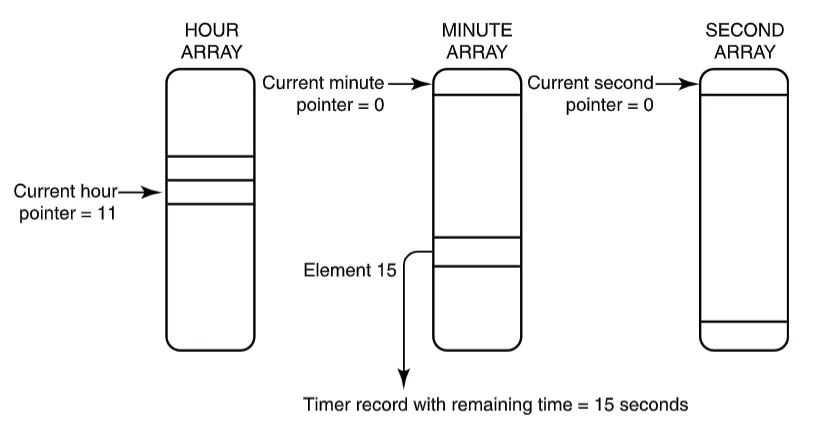
\includegraphics[width=0.8\textwidth]{../assets/ch01/ch01-1_5_端_定时器-004.png}
\end{figure}
图7.4方案7使用的分层列表数组，用于更高效地 “映射” 时间
7.6 分层轮
基本方案的第二种扩展利用了分层的概念。为了表示数字1000000，我们只需要7位数字，而不是
1000000个数字，因为我们以1、10、100等为单位分层表示数字。同样，为了表示32位范围内的所有可
能定时器值，我们不需要一个有 232 个元素的数组。相反，我们可以使用多个不同粒度的数组。例如，
我们可以使用以下四个数组：
  ● 一个有100个元素的数组，每个元素代表一天；


                                                   9
 ●  一个有24个元素的数组，每个元素代表一小时；
  ● 一个有60个元素的数组，每个元素代表一分钟；
  ● 一个有60个元素的数组，每个元素代表一秒。

因此，要存储长达100天的定时器，我们不需要 100 × 24 × 60 × 60 = 864 万个存储位置，而只需要
 100 + 24 + 60 + 60 = 244 个位置。
例如，看图7.4。假设当前时间是11天10小时24分30秒。要设置一个50分钟45秒的定时器，我们首先计
算定时器到期的绝对时间，即11天11小时15分15秒。然后，我们将定时器插入到小时数组中，位于当前小
时指针（10）向前1（11 - 10小时）个元素的列表中。我们还将余数（15分钟15秒）存储在这个位置。在
图7.4中展示了这一过程，为简化示例，忽略了在该示例中未发生变化的日期数组。
秒数组的工作方式与通常一样：每次硬件时钟滴答时，我们递增秒指针。如果该元素指向的列表不为
空，我们对列表中的元素执行EXPIRYPROCESSING操作。然而，其他三个数组的工作方式略有不同。
即使服务的用户没有请求任何定时器，也总会有一个60秒的定时器用于更新分钟数组，一个60分钟的定
时器用于更新小时数组，以及一个24小时的定时器用于更新日期数组。例如，每次60秒定时器到期时，
我们将递增当前分钟定时器，对分钟定时器执行任何必要的EXPIRYPROCESSING操作，并重新插入另
一个60秒定时器。
回到前面的例子，如果定时器未停止，最终小时定时器将到达11。当小时定时器到达11时，会检查列表；
EXPIRYPROCESSING将把剩余的秒数（15）插入到分钟数组中，位于当前分钟指针（0）之后的第15个
元素处。当然，如果剩余分钟数为零，我们可以直接进入秒数组。此时，表格看起来将如\begin{figure}[htbp]
\centering
\includegraphics[width=0.8\textwidth]{../assets/ch01/ch01-1_5_端_定时器-005.png}
\end{figure}
图7.5所示。




图7.5前一个例子，但在定时器的小时部分到期后（使用方案7）
最终，分钟数组将到达第15个元素；作为EXPIRYPROCESSING的一部分，我们将把定时器移动到秒数
组中，位于当前值之后的15秒处。15秒后，定时器将实际到期，此时将执行用户指定的
EXPIRYPROCESSING操作。

                                                         10
在方案6和方案7之间做出选择并不容易。对于较小的T值和较大的M值，方案6在STARTTIMER和
PERTICKBOOKKEEPING操作上可能都比方案7更好。然而，对于较大的T值和较小的M值，方案7在
PERTICKBOOKKEEPING的平均成本（延迟）方面会更好，但在STARTTIMER延迟方面成本更高。
需要注意的是，如果允许定时器的精度随着分层级别增加而降低，那么我们就不需要在不同级别之间迁
移定时器。例如，在前面的例子中，我们可以将时间四舍五入到最接近的小时，只设置小时级别的定时
器。当小时定时器到期时，我们执行用户指定的EXPIRYPROCESSING操作，而无需迁移到分钟数组。
本质上，我们现在有了不同的定时器模式，一种用于小时定时器，一种用于分钟定时器，等等。这进一
步降低了PERTICKBOOKKEEPING的开销，但代价是精度损失高达50%（例如，一个1分30秒的定时器
被四舍五入为1分钟）。或者，我们可以通过允许在相邻列表之间仅进行一次迁移来提高精度。
7.7 BSD实现
目前，Linux内核针对本章开头描述的两种不同用例，提供了两种不同的定时器设施。高分辨率定时器
（“hrtimer”）机制为用户提供精确的定时器，这些定时器会运行至完成，例如在速率控制算法中使用。
较低分辨率的定时器用于事件超时和故障推断。虽然高分辨率定时器使用平衡（红黑）树（Gleixner和
Niehaus，2006），但较低分辨率的定时器（Corbet，2015）使用分层定时器，不过，如前所述，它选
择限制定时器迁移（在Linux术语中称为 “级联”（Corbet，2015）），以牺牲精度为代价。早期版本的
Linux（1997年首次实现（Gleixner和Niehaus，2006））只使用了一种方法 —— 带有迁移的分层时间
轮，称为级联时间轮（CTW）。
7.7 BSD实现
Adam Costello率先使用哈希轮实现（Costello和Varghese，1998）了BSD UNIX的调用和定时器设施。
早期的BSD内核在设置或取消定时器时所花费的时间与未完成定时器的数量成正比。而基于方案6的
Costello实现，启动、停止和维护定时器的时间是恒定的；这带来了高度可扩展的设计，能够轻松支持数
千个未完成的定时器，且开销很小。
在最初的BSD实现中，每个调用由一个CALLOUT结构表示，该结构包含一个指向要调用函数的指针
（C_FUNC）、一个指向函数参数的指针（C_ARG），以及一个以时钟滴答为单位表示的时间
（C_TIME）。未完成的调用存储在一个链表中，并根据到期时间进行排序。每个CALLOUT结构的
C_TIME成员是相对时间，而不是绝对时间；链表中的第一个调用存储从现在到到期的滴答数，后续每个
调用存储其自身到期时间与前一个调用到期时间之间的滴答数。
在BSD UNIX中，调用分别使用TIMEOUT()和UNTIMEOUT()来设置和取消。TIMEOUT(FUNC, ARG,
TIME)注册FUNC(ARG)在指定时间被调用。UNTIMEOUT(FUNC, ARG)取消具有匹配函数和参数的调
用。由于对CALLTODO列表进行线性搜索，最初这两个操作所花费的时间都与未完成调用的数量成正
比。在搜索期间，中断被锁定。

                                                               11
在现有系统中添加新算法有时会遇到与现有接口的兼容性问题。例如，Costello实现基于方案6。然而，
Costello发现，BSD中的TIMEOUT()/UNTIMEOUT()接口不允许传递句柄，而在我们上面描述的所有方
案中，传递句柄用于快速取消定时器。Costello实现通过两种解决方案来解决这个问题。对于使用现有接
口的调用，通过哈希表根据函数指针和参数搜索调用。还实现了第二种解决方案：定义了一个新的接口
函数UNSETCALLOUT()，用于删除调用，该函数仅接受一个句柄作为参数。这使得现有代码可以使用旧
接口，而新应用程序可以使用新接口。这两种方法的性能差异很小，因此哈希表方法更受青睐。
在Costello实现中，定时器例程保证仅在一小段有界时间内锁定中断。Costello实现还扩展了
SETITIMER()接口，允许一个进程拥有多个未完成的定时器，从而减少了用户维护自己定时器包的需求。
对BSD内核的更改很小（添加了548行代码，删除了80行代码）。详细信息可在（Costello和
Varghese，1998）中找到；书面报告包含了一些此处未提及的重要实现细节。
多核机器的出现要求对Costello实现进行更改。早期的一项更改是，将单个调用轮替换为每个CPU一个
调用轮，以提高可扩展性和性能（Motin和Italiano，2018）。Motin和Italiano（Motin和Italiano，
2018）最近推出了一个更新版本，称为Calloutng，以解决Costello实现的以下三个缺点。第一，时间间
隔会舍入到下一个时钟滴答，导致精度损失；第二，每次中断都会唤醒CPU，导致额外的能源消耗；第
三，无法延迟和合并调用，从而导致额外的中断。他们考虑过使用平衡树，但最终决定保留轮结构。不
过，代码进行了更新，更加注重精度，允许聚合，使用新的哈希函数对轮进行索引，并仔细考虑了CPU
缓存亲和性的影响（Motin和Italiano，2018）。
7.8 谷歌Carousel实现
在Costello实现多年后，谷歌构建了一个可扩展的流量整形系统，称为Carousel（Saeed等人，
2017），其底层数据结构是一个时间轮，能够处理数十万个并发的细粒度定时器。由于其速度和规模比
Costello实现高得多，我们简要回顾一下推动这种设计的新用例。
第一个用例是在基于速率的拥塞控制算法（如BBR（Cardwell等人，2017））中使用精细的速率调整。
回想一下，TCP拥塞控制算法是基于拥塞信号（如拥塞路由器设置的拥塞标志位和丢弃的数据包）来减
小窗口大小（未确认的字节数）。TCP拥塞控制算法的问题在于，当收到大量字节的累积确认时，发送
方可能会向网络中突发大量流量，这可能导致路由器丢弃数据包。相比之下，基于速率的拥塞算法（如
BBR）根据拥塞信号控制数据包的发送速率。而速率又由精细的定时器控制，这些定时器控制数据包发
送之间的时间间隔。据报道，使用BBR大大改善了全球的往返延迟和YouTube的体验质量指标
（Cardwell等人，2017）。
第二个用例是在服务器中实现虚拟机（VM）隔离，这些服务器托管着数千个虚拟机，每个虚拟机可以与
数百个其他虚拟机进行通信。如果不对每个虚拟机单独或总体使用的带宽进行限制，一旦某个虚拟机以
过高的速率发送数据，其他虚拟机可能会受到不利影响，因为它们共享相同的物理出站链路。第三个用
例与数据中心计算中的Incast问题（Saeed等人，2017）类似，在这种情况下，一个请求会收到来自其他

                                                                12
服务器的数百个响应，这会导致路由器丢弃数据包。通过让繁忙的接收方使用精细的速率调整来控制其
发送回的确认消息，可以缓解Incast问题。
第二个和第三个用例传统上是通过令牌桶方案来实现的，我们将在关于路由器QoS的第14章中描述该方
案。简而言之，其思想是为每个用户分配一定数量的令牌，用户在每个定时器时钟周期可以使用这些令
牌发送字节数。当用户发送的字节数超过其拥有的令牌数时，用户的流量要么被丢弃（在这种情况下称
为策略器），要么被放入队列中，直到有更多令牌到达（在这种情况下称为整形器）。虽然这种方案传
统上在路由器中实现，但上述三个用例需要在主机中使用令牌桶。例如，Linux的流量控制组件Qdisc
（Components of Linux Traffic Control）支持不同的公平队列策略，包括HTB（hierarchical token
buckets）。
对谷歌服务器的测量（Saeed等人，2017）表明，在Linux中使用现有的Qdisc机制，要么导致速率控制
不完善，要么造成过高的CPU开销。因此，Carousel的设计者（Saeed等人，2017）没有依赖Linux的定
时器，而是采用了大型哈希时间轮。 然而，Carousel并非定时器工具，而是一种能够扩展到处理数十万
个流量的流量整形器/策略器。为避免流量整形器中出现应用程序持续突发数据包并在Carousel中排队的
问题，Carousel系统还引入了一种称为延迟完成的概念。 延迟完成的理念是，在Carousel将存储的数据
包发送到网卡之前，不允许系统调用完成。这就提供了一种反馈机制，能够让过于激进的发送方降低发
送速度。延迟完成意味着完成情况可能会乱序到达 —— 一个速率设定较慢的应用程序，即便其请求发送
得更早，却可能比速率较快的应用程序更晚收到完成通知。这就需要使用哈希表（P15）来匹配完成情况
和请求，虽然增加了复杂性，但却很有价值。因此，延迟完成是一种更改接口的方式（P9）。 需要注意
的是，与传统使用定时器来触发重传或检测故障的场景不同，Carousel中的定时器总是会到期（不像重
传定时器或故障检测定时器，它们几乎不会到期），所以Linux定时器工具中采用的一些优化方法（见
Corbet，2015）无法在Carousel中使用。相反，Carousel采用了其他几种实现技巧。Carousel为每个
CPU配备一个时间轮，以避免锁竞争，并且在必要时可以利用多个内核。它还使用预分配缓冲区
（P2a）来降低缓冲区分配的开销。 最终结果是，Carousel对谷歌流量的整形精度比早期最好的流量整
形技术提高了10倍（Saeed等人，2017），同时将整体机器的CPU利用率提高了10%，内存使用量相比
早期技术降低了两个数量级。这表明，将时间轮从根本上融入到流量整形算法中（而不仅仅作为定时器
工具使用），再结合延迟完成等创新技术，能够发挥巨大的作用。
7.9 获取更细粒度的定时器
随着网络速度的提升，人们可能会认为，随着到目的地的往返延迟减少，重传定时器的时长也会相应缩
短。如果往返延迟降至微秒级别，那么重传定时器也降至微秒级似乎是合理的。但遗憾的是，在大多数
操作系统中，即便往返延迟已降至微秒级，人们仍只能使用毫秒级的定时器。虽然时间轮的使用能够实
现更细粒度的重传定时器，但定时器的粒度仍然无法小于定时器的时钟周期。
如今，许多CPU都配备了可编程的硬件中断芯片，可将其编程为以所需频率中断CPU。因此，一种看似
简单的提高定时器分辨率的方法是增加时钟中断的频率。结合时间轮的使用，这似乎能够提供更细粒度
的定时器。
                                                                       13
然而，这个方法存在一个缺陷。正如我们在模型部分所讨论的，现代CPU为了加快处理速度会保存大量
状态信息，这其中包括流水线状态、大量寄存器的使用，以及缓存和页表缓存（TLB）。中断会带来高
昂的开销，因为它涉及到CPU状态的保存和恢复，并且可能会改变局部性模式，导致在退出中断处理程
序后出现缓存和TLB缺失的情况。Aron和Druschel在1999年进行的早期测量表明，在300或500MHz的
奔腾处理器上，一次中断的成本约为4.5微秒。更糟糕的是，随着处理器速度的提升，并没有迹象表明中
断处理时间会有所改善。
因此，更频繁的硬件中断会导致过多的开销。就目前定义的问题而言，如果将定时器模块视为一个黑
盒，我们似乎找不到解决方案。不过，系统思维通过再次考虑P4原则并利用其他系统组件，为我们的困
境提供了解决方案。要知道，CPU的运行过程中充满了其他类型的转换事件，这些事件涉及到状态的保
存和恢复以及局部性模式的改变。这类转换事件包括系统调用（例如，对设备驱动程序的调用）、异常
（例如，页面错误）以及硬件中断（例如，来自网络适配器的中断）。
如果我们将检查过期定时器作为这类转换事件代码的一部分，那么状态保存和局部性改变的开销已经包
含在转换事件中，不会因定时器处理程序而显著增加。这是有利的一面。但不幸的是，与硬件时钟中断
不同，转换事件的频率是不可预测的。这是不利的一面。
不过，Aron和Druschel在1999年对广泛的基准测试进行的实验表明，转换事件之间的平均延迟在5到30
微秒之间，具体取决于CPU正在运行的任务；延迟超过100微秒的情况仅占6%，并且最大延迟从未超过1
毫秒。
这些数据表明了P3原则的一种有趣应用，即放宽系统要求。我们不再提供总是能提供微秒级定时器的
“硬” 定时器设施，而是提供一种 “软” 定时器（Aron和Druschel，1999）设施，它通常能提供10微秒的
定时器。我们还可以通过每1毫秒添加一次硬件时钟中断来限制软定时器设施的误差。因此，软定时器对
于那些能从预期情况（P11）下几十微秒的定时以及最坏情况下1毫秒的定时中受益的应用程序来说是有用
的。
幸运的是，大多数使用定时器的应用程序都能从这种近似定时器中受益。以故障恢复中的快速重传为
例，如果除了偶尔的一次重传需要1毫秒外，大多数重传都很快，那么故障恢复性能将会得到提升。再考
虑控制某些实体产生速率的算法，只要算法的正确性能够容忍速率的变化或抖动，那么在预期情况下性
能应该会有所提高。例如，Aron和Druschel在1999年展示了如何通过速率控制使TCP连接大致每12微秒
发送一个数据包。更精细的速率控制减少了数据的突发性，但速率的偏差并不影响其正确性。
最后，或许处理微秒甚至纳秒级定时器的正确方法是添加硬件（P5）。这种硬件可以是一个定时器芯
片，它使用时间轮或d -堆在芯片内部完全处理所有定时器。这样，芯片内部有一个硬件时钟，硬件时钟
中断在芯片内部处理；只有当定时器到期时，CPU才会被中断。然而，如果定时器经常被取消，CPU与
芯片通信以取消定时器可能会带来相当大的开销。
7.10 结论

                                                        14
本章介绍了两种高效实现定时器的技术。第一种技术是时间轮，它将定时器实现的开销降低到恒定时
间，而与未完成定时器的数量无关。这使得定时器设施能够提供大量定时器，对于如今的互联网服务器
而言，这是一个非常有用的特性，因为这些服务器有时需要为数千个并发客户端提供服务。第二种技术
是软定时器，它减少了PERTICKBOOKKEEPING操作所带来的操作系统开销。这使得定时器设施在预期
情况下能够提供细粒度的定时器，随着互联网链路速度的提升，这一特性非常实用。这两种方案所使用
的原理总结在表7.1中。
当时间轮在1987年首次被提出（Varghese和Lauck，1987）时，人们普遍认为它解决的是一个无关紧要
的问题。正如当时一位系统设计师所说：“如果它没坏，为什么要修呢？”——这是一个合理的问题。然
而，思考那些你预测未来可能出现的问题的解决方案是很有帮助的。以下信息改编自Justin Gibbs
（FreeBSD早期的关键实现者之一）的言论，不过其中关于实际产品使用的内容有些过时。
在本书第一版中引用了Gibbs的话，他说在那个时候，雅虎通过分布在全球的500台FreeBSD服务器提供
所有内容服务。同样在那个时候，最大的基于网络的电子邮件服务提供商Hotmail最初在电子邮件路由和
网络服务中都使用了FreeBSD。此外，包括美国两家最大的互联网服务提供商Best Internet和USWest在
内的数千家互联网服务提供商，在那个时代都依赖FreeBSD为用户提供互联网新闻服务、数据包路由、
网站托管和shell服务。
然而，在1997年下半年，情况变得很明显，FreeBSD内核中使用的定时器服务很快将成为系统吞吐量的
瓶颈。定时器事件被用于多个需要基于事务的时间通知的应用程序中。随着事务数量和 / 或频率的增
加，定时器接口的负载呈线性增长。例如，FreeBSD内核过去会为每个磁盘事务安排一个 “看门狗” 定时
器，如果定时器触发，就会启动错误恢复操作。在一台典型的服务器上，在250个并发磁盘事务的适度负
载下，超过15% 的CPU资源被定时器事件调度所占用。对旧定时器接口所采用算法的分析表明，CPU负
载会随着并发事务数量的增加而线性上升，这损害了系统的可扩展性。
Justin Gibbs在发现并修复了Costello实现中的一个错误后，在FreeBSD中实现了哈希轮。他的实现将
FreeBSD基准测试中的定时器开销降低到了总CPU使用率的一小部分。Costello算法确保了无论事务负
载如何，开销都接近恒定，保证了定时器设施能够轻松扩展以处理数千个事务。虽然BSD代码后来针对
多核机器进行了更新，并且Motin和Italiano在2018年也进行了进一步更新，但二十年后，哈希轮的基本
用法仍然存在。
许多其他操作系统，如Linux，现在也使用时间轮，大多数实时操作系统（包括路由器中使用的操作系
统）也是如此。需要注意的是，Linux提供了两种定时器设施：一种是粗粒度定时器（Corbet，2015），
它使用分层时间轮，但限制了时间轮之间的迁移（在Linux术语中称为 “级联”）；另一种是高分辨率定
时器（Gleixner和Niehaus，2006），它使用红黑树。最后，现代云操作系统在对数十万个流量进行非
常精细粒度的可扩展流量整形时，也使用哈希轮，因为哈希轮能够在低CPU开销的情况下实现更精确的
流量整形（Saeed等人，2017）。从长远来看，关注算法设计是会有回报的。



                                                        15


\chapter{端系统：协议处理}
% 来源: 19c9fbd0-f942-820b-8000-0000ce63f48e_1.7_端_协议处理.pdf
% 提取时间: 2026-02-28T22:51:53+08:00

1.7 端：协议处理
第9章 协议处理
我们脑海中音乐家的形象往往与举办独奏音乐会联系在一起，而研究人员的形象可能是在仔细思考某个
问题。然而，音乐家更多时间花在一些不那么光鲜的任务上，比如练习音阶，研究人员也会在诸如撰写
经费申请这类日常琐事上花费比预期更多的时间。要精通一项职业，就必须关注许多小任务，而不仅仅
是少数大工作。
同样地，关于高效协议实现的教程通常会强调避免数据处理开销的方法以及减少控制开销的结构化技
术。当然，这些内容在第5章和第6章中已经有所涉及。这是完全合理的，因为终端节点实现的最大改进
往往来自于对这些开销的关注。
然而，在创建了零拷贝且上下文切换极少的实现后（有充分证据表明现代网络设备的实现已经很好地吸
取了这些经验教训），新的瓶颈又引发了人们的审视。事实上，凯（Kay）和帕斯夸莱（Pasquale）在
1993年进行的一项测量研究表明，这些其他瓶颈可能相当显著。
还有许多其他协议实现任务可能成为新的瓶颈。第7章和第8章已经讨论了高效的定时器和多路分解实
现。本章将简要介绍一些常见的剩余任务：缓冲区管理、校验和计算、序列号管理、重组以及通用协议
处理。
这些协议处理 “琐事” 的重要性可能会因以下原因而日益增加。第一，本地网络的链路速度已经达到千兆
级别，并且还在不断提升。第二，市场压力促使人们在硬件中实现传输控制协议（TCP），甚至更高级
别的应用任务，如网络服务和可扩展标记语言（XML）。第三，互联网上存在大量小数据包，对于这些
数据包而言，数据操作开销可能并非主要因素。
本章的结构如下。9.1节深入探讨缓冲区管理技术，即快速缓冲区分配和缓冲区共享技术。9.2节介绍循环
冗余校验（CRC，主要在链路层）和校验和（主要在传输层）的实现技术。9.3节以TCP和用户数据报协
议（UDP）为例，讨论通用协议处理的高效实现。最后，9.4节涵盖数据包重组的高效实现。
本章介绍的技术（以及相应的原则）总结在表9.1中。
 编号               原则              应用场景
 P4b              使用线性缓冲区，而非mbuf链 Linux的sk_buf
                  表
 P4b              不进行合并的伙伴系统      BSD 4.2的malloc()函数
 P2b              顺序块分配，延迟块创建     J机器

                                                   1
P14                高效的缓冲区窃取       随机公平排队（SFQ）
P13                动态缓冲区阈值        -
P2a                使用查表法一次计算多个位的 许多CRC芯片
                   CRC
P2b                延迟进位评估         快速校验和计算
P12a               重新计算头部校验和      RFC 1624
P4c                计算数据链路和应用层的CRC 无限带宽（Infiniband）
P11                预测下一个TCP头部     BSD的TCP协议
P3c                将分片操作从路由器转移到源端 路径最大传输单元（Path
                                  MTU）
P11                快速分片重组         -
P6                 创建高效的专用例程      UDP校验和计算

快速参考指南
9.1节的第一部分描述了多种缓冲策略，包括UNIX的mbufs和Linux的sk_bufs，以及各种高效的内存分配
器，如金斯利（Kingsley）分配器。对快速循环冗余校验（CRC）算法感兴趣的实现者可以阅读9.2.1
节；对快速IP校验和感兴趣的人应该阅读9.2.2节。9.3节的前几页描述了经典的TCP处理优化方法——头
部预测。
9.1 缓冲区管理
所有协议都必须管理缓冲区。尤其是数据包在协议栈中上下传输时都存放在缓冲区里。操作系统必须提
供分配和释放缓冲区的服务。这需要管理空闲内存，找到合适大小的内存可能颇具挑战，特别是因为缓
冲区分配必须实时完成。9.1.1节介绍了一种简单的系统解决方案，即使对于大小可变的请求，也能实现
高速缓冲区分配。
如果空闲空间必须在多个连接或用户之间共享，那么提供某种公平机制也很重要，这样单个用户就无法
独占所有资源。虽然静态限制能起到一定作用，但在某些情况下，动态缓冲区限制可能更可取，即一个
进程在单独运行时可以获取所需的任意数量的缓冲区，但当其他进程到来时，它会释放多余的缓冲区。
9.1.2节介绍了两种可以高速实现的动态缓冲区限制方案。
9.1.1 缓冲区分配
                                                        2
经典的BSD UNIX实现使用mbufs，它允许将单个数据包存储为较小缓冲区的线性列表，其中每个缓冲区
是一块连续的内存区域。这种技术的动机是允许分配给数据包的空间能够动态增长和收缩（例如，当数
据包在协议栈中上下传输时）。例如，通过在当前的mbuf链表前添加一个新的mbuf来扩展数据包的空间
很容易。为了实现更大的灵活性，BSD mbufs有三种类型：两种小尺寸（100字节和108字节）和一种大
尺寸（2048字节，称为簇）。
除了允许数据包分配的内存动态扩展外，mbufs还能有效地利用内存，这在1981年左右mbufs发明时非常
重要。例如，一个190字节的数据包将被分配两个mbuf（大约浪费20字节），而一个450字节的数据包
将被分配五个mbuf（大约浪费50字节）。
然而，数据包大小的动态扩展可能并不像听起来那么重要，因为重要数据包路径（如以太网、IP、TCP）
的头部大小是已知的，可以预先分配。同样，在如今的工作站中，节省内存可能不如提高数据包处理速
度重要。另一方面，mbuf的实现使得数据访问和复制变得更加困难，因为可能需要遍历链表。
因此，早期范·雅各布森（Van Jacobson）设计了一个原型内核，使用我们称之为pbufs的结构。正如雅
各布森在一封电子邮件中所说（雅各布森，1993年）：“每个pbuf中恰好存放一个连续的数据包（没有那
种mbuf链表的繁琐结构）。”
虽然pbufs已经逐渐被遗忘，但Linux操作系统目前在网络缓冲区中采用了非常类似的概念（考克斯，
1996年），称为sk_buf。这些缓冲区和pbufs一样，是线性缓冲区，并预先为后续可能需要添加的数据包
头部预留了空间。有时，这会为处理最坏情况下的头部大小而浪费一些空间，但更简单的实现方式使得
这种做法是值得的。sk_bufs和pbufs都放宽了缓冲区的规范，以避免不必要的通用性（原则P7），并以
空间换取时间（原则P4b）。
鉴于像Linux中使用线性缓冲区大小是个好主意，那么我们如何为各种大小的数据包分配内存呢？动态内
存分配通常是一个难题，因为用户（例如TCP连接）在不同时间释放内存，这些释放操作可能会将内存
碎片化，形成大小各异的空洞。
标准教科书算法，如首次适配（First-Fit）和最佳适配（Best-Fit）（威尔逊等人，1995年），实际上
是在内存中逐个查找，寻找合适大小的空洞。任何实现高速网络（如TCP）的人员，一想到使用这样的
分配器都会感到恐惧。相反，应该考虑以下三种分配器。
  ● 分离池分配器：克里斯·金斯利（Chris Kingsley）开发的一种分配器是最快的分配器之一，它与
    BSD 4.2 UNIX一起发布。金斯利的malloc()实现将所有内存划分为一组以2的幂次方大小划分的分离
    内存池。任何请求都会向上取整到最接近的2的幂次方，通过查表找到相应的内存池列表，如果列表
    中有可用缓冲区，则从列表头部分配一个缓冲区。之所以称这些内存池是分离的，是因为当某个大
    小的请求失败时，不会尝试分割可用的较大缓冲区或合并相邻的较小缓冲区。
这种分割和合并操作实际上是由一种更经典的方案——伙伴系统来完成的（关于内存分配器的全面回
顾，见威尔逊等人，1995年）。不进行这些操作显然会浪费内存（原则P4b，以内存换取速度）。如果
所有请求的大小都恰好对应一个内存池的大小，那么其他内存池就会被浪费。然而，这种限制并不像看
起来那么糟糕，因为使用伙伴系统的分配器在最坏情况下的表现要糟糕得多。
                                                         3
例如，假设所有请求的大小都是1，并且每隔一个缓冲区就被释放。那么，使用伙伴系统时，内存会退化
为一系列大小为1的空洞，后面跟着一个大小为1的分配。一半的内存未被使用，但任何大于2的请求都无
法得到满足。请注意，这个例子不会发生在金斯利分配器中，因为大小为1的请求只会耗尽大小为1的内存
池，而不会影响其他内存池。因此，不同内存池之间的资源调配可能有助于提高预期的内存利用率，但
无法改善最坏情况下的利用率。
  ● Linux分配器：Linux分配器（切尔夫，2001年）最初由道格·利（Doug Lea）编写，有时也被称为
    dlmalloc()。与金斯利分配器类似，它将内存划分为128种大小的内存池。前64个内存池分别包含大
    小固定的内存缓冲区，从16字节到512字节，以8字节为步长递增。与2的幂次方分配方式不同，这种
    方式在常见的小缓冲区情况下，浪费的空间不会超过8字节。剩下的64个内存池涵盖其他更大的尺
    寸，按指数间隔分布。
Linux分配器（切尔夫，2001年）会合并相邻的空闲缓冲区，并将合并后的缓冲区提升到合适的内存池。
这与伙伴系统类似，因此也会面临与任何不分离内存池方案相同的碎片化问题。然而，在实际应用中，
其内存利用率非常高。
有一个实用的技巧可以记在心里，就是关于内存池如何链接在一起。简单的做法是为每个内存池创建单
独的空闲列表，使用额外的小节点指向相应的空闲缓冲区。但由于缓冲区是空闲的，这显然是一种浪费
（原则P1）。因此，在Linux以及其他可能的分配器中使用的简单技巧是，将内存池空闲列表的链接指针
存储在相应的空闲缓冲区本身中，从而节省存储空间。
利分配器比金斯利分配器更有效地利用内存，但实现起来更复杂。对于既追求速度又追求内存高效利用
的线速TCP实现来说，这可能不是最佳选择。
  ● 批量分配器：另一种内存分配的替代方案是批量分配（原则P2c），其硬件实现比金斯利分配器更简
    单。如\begin{figure}[htbp]
\centering
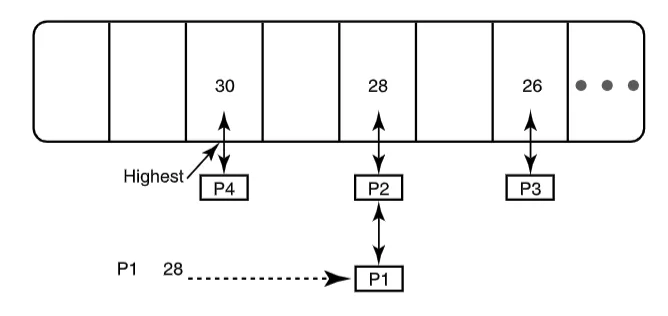
\includegraphics[width=0.8\textwidth]{../assets/ch01/ch01-1_7_端_协议处理-001.png}
\end{figure}
图9.1所示，这种分配器的工作方式是在大的内存块中进行分配。每个内存块按顺序分配，有
    一个指针Curr指向最后一次分配结束的位置。大小为B的新请求在Curr之后进行分配，然后Curr增加
    到Curr + B。这种方式速度极快，能处理可变大小的请求，并且在内存块被用完之前不会浪费任何
    内存。
其思路是，当一个内存块用完时，另一个内存块可以立即使用。当然，天下没有免费的午餐，在使用第
二个内存块时，必须在后台创建一些备用内存块。备用内存块的创建可以由软件完成，而分配操作可以
很容易地在硬件中实现。类似的想法在麻省理工学院的J机器（达利等人，1987年）中也有体现，J机器
依赖于底层的快速消息传递服务。
创建备用内存块有很多方法。当然，问题在于释放操作的顺序可能与分配操作不同，这会在内存块中产
生一组空洞，需要以某种方式进行合并。有三种合并空洞的方法。如果应用程序知道最终所有分配的缓
冲区都会被释放，那么使用更多的备用内存块可能就足以确保在任何一个内存块用完之前，有某个内存
块能被完全清理出来。然而，这是一种有风险的做法。


                                                         4
图9.1 从大内存块中顺序分配并使用备用内存块。其巧妙之处在于利用完全分配一个内存块所需的时间来
创建一个新的内存块。
其次，如果内存是通过间接寻址访问的，比如在虚拟内存中，并且缓冲区是在虚拟内存中分配的，那么
可以使用页面重映射将许多分散的物理内存页面聚集在一起，使其看起来像一个连续的虚拟内存块。最
后，还可以考虑内存压缩。在像UNIX这样的通用分配器中，内存压缩显然是不可接受的，因为可能有任
意数量的内存块指向一个内存节点。然而，在使用缓冲区或其他树状结构的网络应用中，使用简单的局
部压缩方案（西卡和瓦格赫斯，2000年），内存压缩可能是可行的。
9.1.2 共享缓冲区
如果说缓冲区分配已经够难了，那么再加上公平性约束，就更具挑战性了。假设一个实现希望在多个用
户之间公平地共享一组缓冲区，每个用户都可能希望使用所有的缓冲区。这些缓冲区应该大致平均地分
配给需要它们的活跃用户。这类似于经济学中的帕累托最优，也与第14章中研究的路由器公平排队要求
相似。因此，在随机公平排队（SFQ）算法的背景下发明了以下缓冲区窃取算法（麦肯尼，1991年）也
就不足为奇了。
 ● 缓冲区窃取：一种在用户之间大致实现帕累托最优的方法如下。当所有缓冲区都被用完，而一个新
   用户（其分配的缓冲区比当前最大分配量小）还想要一个缓冲区时，就从拥有最多缓冲区的用户那
   里窃取一个额外的缓冲区。很容易看出，即使一开始某个用户占用了所有缓冲区，当其他用户变得
   活跃时，他们也可以通过窃取获得公平的份额。
问题在于，缓冲区窃取问题的一般解决方案需要使用堆。堆的时间复杂度为O(log n)，其中n是当前有分
配的用户数量。如何才能加快速度呢？
同样，在算法学与算法的对比中，问题往往源于对规范的过度解读。如果分配量不断以任意增量变化，
并且算法总是希望找到最大的分配量，那么就需要使用对数堆实现。然而，如果我们可以放宽规范（在
实际中这似乎是合理的），假设用户每次只窃取一个缓冲区，那么分配量的变化就不是任意的，而只是
增加或减少1。这一观察结果产生了一种常数时间算法（麦肯尼算法，\begin{figure}[htbp]
\centering
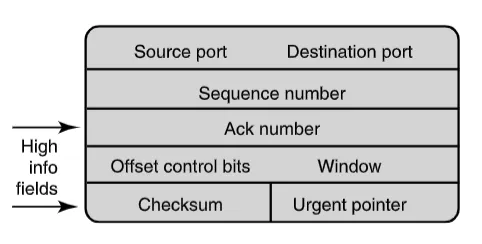
\includegraphics[width=0.8\textwidth]{../assets/ch01/ch01-1_7_端_协议处理-002.png}
\end{figure}
图9.2），该算法还假设缓冲区分配

                                                 5
量落在一个有限的集合内。对于每个分配大小i，该算法维护一个包含所有分配大小恰好为i的进程的列
表。算法还维护一个名为Highest的变量，它指向任何进程的最大分配量。
当进程P希望窃取一个缓冲区时，算法会在Highest指向的列表头部找到分配量最大的进程Q。在此过程
中，进程P获得一个缓冲区，进程Q失去一个缓冲区。记录更新如下：当进程P获得缓冲区i + 1时，P从列
表i中移除并添加到列表i + 1中，必要时更新Highest。当进程Q失去缓冲区i + 1时，Q从列表i + 1中移除
并添加到列表i中，如果Highest指向的列表变为空，则更新Highest = i。
请注意，如果P和Q的分配量变化大于1，这个算法可能会变得效率极低。例如，如果Q的分配量减少
100，并且没有其他用户具有相同的原始分配量，那么算法将需要遍历100个列表，寻找下一个可能的最
大分配量。由于分配量的最大变化量为1，所以算法只需要遍历一个列表。从算法学的角度来看，这是利
用有限全域创造特殊机会的一个例子（原则P14建议对有限全域使用桶排序和位图）。




图9.2 麦肯尼缓冲区窃取算法利用每次操作缓冲区值最多变化1这一事实，巧妙地避免了对数堆带来的开
销。
 ● 动态阈值：在共享内存交换机（第13章）中，限制任何一个流对共享缓冲区的访问也很重要。在共
   享内存交换机的背景下，乔杜里（Choudhury）和哈内（Hahne）描述了一种类似于缓冲区窃取的
   算法，他们称之为Pushout。然而，即使使用麦肯尼（1991年）的缓冲区窃取算法，Pushout在高速
   实现时可能也很困难。
相反，乔杜里和哈内（1998年）提出了一种有用的替代机制，称为动态缓冲区限制。他们观察到，为每
个流维护一个固定的阈值，要么限制过度（如果阈值太小），要么过于危险（如果阈值太大）。使用固
定的阈值与使用固定窗口大小进行流量控制没有区别。但是TCP使用动态窗口大小来适应拥塞情况。同
样，利用自由度（原则P13）并使用动态阈值是有意义的。
直观来讲，TCP窗口流量控制机制会在出现未被使用的带宽（通过数据包无丢失情况来衡量）时，增大
连接的窗口大小。同样，在共享缓冲区中适应拥塞的最简单方式，是监测剩余的空闲空间，并根据空闲
                                                          6
空间的大小按比例提高阈值。因此，用户所使用的空间被限制在不超过$cF$字节，其中$c$为常数，
$F$是当前的空闲空间量。如果将$c$选为2的幂次方，该方案仅需使用一个移位器（用于乘以$c$ ）和
一个比较器（用于与$cF$进行比较）。这甚至比缓冲区窃取算法要简单得多。
乔杜里（Choudhury）和哈内（Hahne）推荐$c$的值为1。这意味着单个用户被限制使用不超过可用带
宽的一半。这是因为当用户使用了一半带宽时，剩余的空闲空间就等于该用户的分配量，此时阈值检查
就会不通过。同样地，如果$c = 2$，任何用户被限制使用不超过可用缓冲区空间的$\frac{2}{3}$。因
此，与缓冲区窃取算法不同，这种方案总是会为新到来的用户预留一些空闲空间，用略微欠佳的内存使
用效率来换取更简单的实现方式。
现在假设有两个用户，且\(c = 1\)。有人可能会天真地认为，既然每个用户被限制使用不超过一半的资
源，那么两个活跃用户就只能使用四分之一的资源。然而，该方案的表现更好。现在每个用户可以使用
三分之一的资源，还剩下三分之一的空闲资源。接下来，如果有两个新用户到来，而老用户不释放他们
的缓冲区，那么这两个新用户最多可以获得九分之一的缓冲区空间。
因此，与缓冲区窃取算法不同，这种方案在短期内并不公平。然而，如果同一组用户存在的时间足够
长，从长期来看，这种方案应该是公平的。在前面的例子中，当分配给前两个用户的缓冲区被释放后，
应该会产生更公平的分配结果。
9.3 通用协议处理
9.1节介绍了数据包的缓冲技术，9.2节介绍了高效计算数据包校验和的技术。现在，我们可以着手实际处
理这样的数据包了。不熟悉TCP的读者可能需要先查阅第2章中的相关模型。
由于在大多数站点中，TCP流量占比达90%（布劳恩，1998年），因此以接近线速高效处理TCP数据包
至关重要。遗憾的是，乍一看，TCP代码令人望而生畏。虽然TCP发送方代码相对简单，但史蒂文斯
（1994年）指出：“TCP输入处理是我们在本文中研究的最大代码块。tcp_input函数大约有1100行代
码。处理传入的段并不复杂，只是冗长且繁琐。”
鉴于TCP看起来较为复杂，格雷格·切森（Greg Chesson）和拉里·格林（Larry Green）在1987年成立
了Protocol Engines公司，并提出了一种名为XTP的替代协议（切森，1989年）。XTP经过精心设计，
其数据包头部易于解析，处理路径也经过优化。随着XTP对TCP构成替代威胁，范·雅各布森（Van
Jacobson）在BSD UNIX中精心调整了TCP的实现，这在史蒂文斯（1994年）的著作中有详细描述。该
实现甚至能够跟上100 Mbps的链路速度。结果，尽管XTP仍在使用（切森，1989年），但TCP取得了巨
大的成功。
雅各布森优化实现的核心是一种称为头部预测的机制（雅各布森，1993年）。在处理这1100行TCP接收
处理代码时，大部分复杂性源于处理罕见情况。头部预测通过优化常见情况（原则P11），为穿越复杂的
异常情况提供了一条快速路径。
9.3.1 TCP头部预测
                                                           7
接收TCP数据包时的第一个操作是找到协议控制块（PCB），其中包含该数据包所属连接的状态（例如
接收和发送序列号）。假设连接已建立，并且大多数工作站只有少数几个并发连接，那么可以缓存这些
活动连接块。BSD UNIX代码（史蒂文斯，1994年）维护一个“滞后一个”的缓存，其中包含最后接收段
的PCB；在实际的工作站实现中，这种方法效果良好。
找到PCB后，必须处理TCP头部。帕特里奇（Partridge，1993年）提出了一种理解头部预测的有效方
式，即查看TCP头部中的字段，如\begin{figure}[htbp]
\centering
\includegraphics[width=0.8\textwidth]{../assets/ch01/ch01-1_7_端_协议处理-007.png}
\end{figure}
图9.7所示。
连接建立后，目的端口和源端口固定不变。由于IP网络会尽力按顺序发送数据包，序列号很可能是最后
接收数据包的序列号的下一个。控制位（通常称为标志位）通常为关闭状态，但确认（ack）位除外，在
发送初始数据包后，ack位始终为开启状态。最后，大多数情况下，接收方不会更改其窗口大小，紧急指
针也无关紧要。因此，信息含量较高的只有确认号和校验和字段。
基于这一观察，头部预测将常见情况确定为以下两种可能之一：接收纯确认数据包（即接收的段不包含
数据）或接收纯数据数据包（即接收的段包含的ack字段不传达新信息）。此外，数据包还应在以下精确
意义上反映正常情况：没有设置意外的TCP标志位，并且数据包中通告的流量控制窗口应与接收方先前
通告的窗口相同。用伪代码表示（简化自雅各布森，1993年）：




图9.7 TCP头部字段：最可能变化的字段是校验和和确认字段。其他字段携带的信息很少，通常可以根据
过去的值进行预测。
  1   IF (无意外标志位) AND (数据包中的窗口与之前相同)
  2      AND (数据包序列号为下一个预期值) THEN
  3           数据包仅包含头部且无数据)
           IF (
  4           执行确认处理
  5           /* 释放已确认字节，停止定时器，唤醒进程 */
  6       ELSE IF (数据包未确认任何新内容) /* 纯数据 */
  7           将数据复制到用户缓冲区，同时计算校验和；
  8           更新下一个预期序列号；
  9           如有需要，发送确认并释放缓冲区；
 10       ENDIF
 11   ELSE /* 头部预测失败 -- 采用常规处理路径 */


                                                    8
显然，这段代码比完整的TCP接收处理代码短得多。然而，利用大多数机器能够以机器字大小为单位进
行高效比较这一事实（原则P4a，利用局部性），可以使一些检查更高效。
例如，考虑图9.7控制位中的TCP标志位。共有六个标志位，每个标志位都编码为一个比特：同步
（SYN）、结束（FIN）、复位（RESET）、推送（PUSH）、紧急（URG）、确认（ACK）。在正常情
况下，除了ACK必须设置且PUSH无关紧要外，所有标志位都应清零。单独检查每个条件需要执行多条指
令来提取和比较每个比特。
相反，可以注意到标志位字段是TCP头部的第四个字，并且窗口大小包含在最后16位中。在头部预测代
码中，发送方预先计算（原则P2a）这个字的预期值，方法是填充所有预期的标志位值，并使用上次通告
的窗口大小。
TCP头部第四个字的预期值存储在连接的PCB条目中。在这种设置下，前面伪代码中的前两个检查可以
通过将传入数据包中TCP头部的第四个字与PCB中存储的预期值进行比较，一次性完成。如果一切顺利
（测试表明通常如此），则仅在连接开始时计算第四个字段的预期值。正是这个测试解释了“头部预
测”这个名称的由来：对头部的一部分进行预测，并与传入的段进行比对。
前面描述的伪代码源自雅各布森在研究内核中的实现（雅各布森，1993年），据称该实现仅用30条Sun
SPARC指令就能完成TCP接收处理！史蒂文斯（1994年）给出的BSD UNIX代码稍微复杂一些，因为它
必须处理mbufs，并且需要排除其他可能性，例如PAWS（TCP序列号回绕）测试（史蒂文斯，1994
年）。
到目前为止，我们的讨论仅限于TCP接收处理，因为它比发送TCP段更复杂。然而，发送方也存在与头
部预测类似的机制。如果各个段之间只有少数字段发生变化，发送方可以从在连接块中保留一个模板
TCP（和IP）头部中受益。发送段时，发送方只需将变化的少数字段填充到模板中。如果复制TCP头部比
逐个填充每个字段更高效，那么这种方法就更具优势。Linux内核中实现了发送数据包头部的缓存机制。
在结束这个话题之前，值得回顾注意事项Q8，并审视这种优化对系统环境的敏感程度。最初，头部预测
是针对工作站设计的。其基本假设（下一个段属于同一连接，并且序列号比最后接收的段的序列号大1）
在这种情况下效果良好。
显然，在服务器环境中，下一个段属于同一连接的假设并不成立。早在雅各布森（1993年）就已指出这
一点，他建议使用端口号的哈希值来快速定位PCB。麦肯尼（McKenney）和多夫（Dove）证实，在在
线事务处理（OLTP）环境中，使用哈希查找PCB可以将接收处理速度提高一个数量级。
先进先出（FIFO）假设更难以绕过。虽然可以采用一些巧妙的方案来处理乱序数据包的序列号，但TCP
中一些更基本的协议机制依赖于FIFO假设。例如，如果数据包经常乱序，TCP接收方会发送重复确认。
在TCP的快速重传算法（史蒂文斯，1994年）中，TCP发送方会根据三个重复确认推断数据包丢失（见
第14章）。
因此，缺乏FIFO行为会导致误重传，与头部预测失败相比，这会更严重地降低性能。然而，随着TCP接
收方逐渐支持选择性确认（弗洛伊德等人，1999年），未来或许能够快速处理乱序段。

                                                    9
9.3.2 UDP处理
回想一下，UDP是没有错误恢复、拥塞控制或连接管理功能的TCP。与TCP一样，UDP通过端口号实现
多路复用和解复用。因此，UDP使应用程序能够在无需处理TCP复杂性的情况下发送IP数据报。尽管
TCP是目前占主导地位的协议，但许多重要应用，如视频会议，都使用UDP。因此，优化UDP实现也很
重要。
由于UDP是无状态的，头部预测并不适用：无法存储过去的头部信息来预测未来的头部。然而，UDP与
TCP有两个可能耗时的相同任务：解复用至正确的PCB以及计算校验和，这两个任务都可以从类似TCP
的优化中受益（帕特里奇和平克，1993年）。
UDP中PCB条目的缓存比TCP中更复杂。这是因为在查找PCB时，可能需要使用通配符条目来匹配远程
（称为外部）IP地址和端口。例如，可能存在PCB 1，它指定本地端口L，而其他所有字段均为通配符；
还可能存在PCB 2，它指定本地端口L和远程IP地址X。如果缓存了PCB 1，而到达的数据包目的地是
PCB 2，那么缓存可能会导致数据包被错误地解复用至PCB 1。因此，一般情况下无法缓存通配符条目；
出于类似原因，在路由查找（第11章）中也不能缓存地址前缀。
帕特里奇和平克（1993年）提出了一种简单策略来解决这个问题。像PCB 1这样可能“隐藏”或匹配其他
PCB条目的条目，绝不允许被缓存。在这个限制条件下，帕特里奇和平克（1993年）的UDP实现会缓存
最后接收数据包的PCB和最后发送数据包的PCB。第一个缓存用于处理连续接收的数据包，而第二个缓
存用于处理常见的情况，即接收到对最后发送数据包的响应。尽管存在缓存限制，但在帕特里奇和平克
（1993年）的测量中，这两个缓存的命中率仍达到87%。
最后，帕特里奇和平克（1993年）还为UDP实现了与TCP类似的复制和校验和循环。在BSD实现中，
UDP的sosend函数被视为通过已连接套接字发送数据的特殊情况。相反，帕特里奇和平克提出了一种高
效的专用例程（原则P6），该例程首先计算头部校验和，然后在将数据字节复制到网络缓冲区的同时更
新校验和。（其中一些想法使Cray机器在20世纪90年代初能够对校验和循环进行向量化处理。）在接收
处理中采用类似的优化措施后，帕特里奇和平克报告称，对于受内存访问时间而非处理能力限制的
CPU，校验和计算的成本基本为零。
9.4 重组
TCP的头部预测以及帕特里奇和平克（1993年）对UDP的优化，都假设接收的数据流无需进行特殊计
算。例如，假设TCP段不包含窗口大小变化或不需要关注的标志位设置。此外，到目前为止，还有一个
未明确说明的假设，即IP数据包无需重组。
简而言之，最初的IP路由协议通过允许路由器将IP数据包分片，来处理具有不同最大数据包大小或最大传
输单元（MTU）的各种链路。每个分片由数据包ID、在原始数据包中的起始字节偏移量和分片长度标
识。最后一个分片会设置一个比特位，以表明它是最后一个分片。需要注意的是，中间路由器可能会导
致一个分片进一步被分割成多个更小的分片。IP路由还可能导致分片重复、丢失和乱序接收。

                                                10
在接收方，“破碎的蛋”（即原始数据包）可以按以下方式重新组装。第一个到达接收方的分片会建立以
相应数据包ID为索引的状态。后续的分片会被引导至相同的状态（例如，基于数据包ID的分片链表）。
如果接收到最后一个分片，并且其余分片覆盖了原始数据包长度中的所有字节（由每个分片的偏移量指
示），接收方就可以判断数据包已完整。如果在指定时间内数据包未完成重组，则该状态将超时。
虽然分片使IP能够处理不同MTU大小的链路，但它存在以下缺点（肯特和莫古尔，1987年）。首先，路
由器对数据包进行分片的成本较高，因为这需要为每个分片添加新的IP头部，从而增加了处理和内存带
宽需求。其次，在终端节点进行重组的成本也较高，因为确定一个完整的数据包是否已组装完成，可能
需要对接收的分片进行排序。第三，一个分片的丢失会导致整个数据包丢失；因此，当一个分片丢失
时，传输其余的分片就是在浪费资源。
当前的互联网策略（肯特和莫古尔，1987年）是将分片计算在空间上（原则P3c）从路由器和接收方转
移到发送方。所谓的路径MTU方案的核心思想是，发送方有责任计算出一个足够小的数据包大小，以确
保数据包能够通过从发送方到接收方路径上的所有链路。现在，路由器可以拒绝分片数据包，并向接收
方发送控制消息。发送方使用常见数据包大小列表（原则P11，优化常见情况），在收到拒绝消息时，从
该列表中选择较小的数据包大小。
路径MTU方案通过将问题转移到系统的其他部分，很好地展示了算法的实际应用。然而，有一种误解认
为路径MTU已完全消除了互联网中的分片现象。事实并非如此。几乎所有核心路由器都支持硬件分片，
并且在路径MTU协议部署多年后，在互联网骨干链路上仍观察到大量分片流量（香农等人，2001年）。
需要注意的是，路径MTU协议要求发送方在PCB中保存当前最佳数据包大小的状态信息。如果发送方使
用TCP，这种方式效果良好，但如果发送方使用无状态的UDP，情况就不同了。在UDP的情况下，只有
当UDP之上的应用程序保存必要的状态并实现路径MTU（除非路径MTU像在IBM AIX系统中那样存储为
路由表条目）时，才能实现路径MTU。这更难部署，因为与仅更改TCP相比，更改众多应用程序更加困
难。因此，在撰写本文时，诸如NFS之类的共享文件系统协议、IP-in-IP封装协议以及许多媒体播放器和
游戏协议都基于UDP运行，并且不支持路径MTU。最后，许多攻击者会将攻击负载分散在多个分片中，
从而危及安全性。因此，入侵检测设备通常必须重组IP分片，以检查重组数据中是否存在可疑字符串。
因此，研究快速重组算法很有必要，因为像NFS这样的常见程序不支持路径MTU协议，并且实时入侵检
测系统必须以线速重组数据包，以检测隐藏在分片中的攻击。下一节将介绍接收方的快速重组实现。
9.4.1高效重组
\begin{figure}[htbp]
\centering
\includegraphics[width=0.8\textwidth]{../assets/ch01/ch01-1_7_端_协议处理-008.png}
\end{figure}
图9.8展示了一种简单的数据结构，类似于BSD UNIX中用于重组数据包的数据结构。假设有三个ID为
1080的数据包分片已经到达。这些分片按照起始偏移量在列表中进行排序。注意，这里存在字节重叠的
情况，因为第一个分片包含字节1-10，而第二个分片包含字节2-21。



                                                  11
图9.8 一种用于重组的数据结构是一个由数据包ID索引、按起始字节偏移量（第一个字段）排序的分片链
表。第二个字段是结束偏移量。因此，起始偏移量为25的分片会插入到列表中第二个元素之后。
因此，如果一个ID为1080、偏移量为25-30的新分片到达，实现过程通常会从列表头部开始遍历，以找
到正确的插入位置。正确的位置在起始偏移量2和40之间，也就是在第二个列表项之后。
每次将一个分片放入列表时，在遍历列表的过程中，实现可以检查到该分片为止是否已经接收到了所有
需要的字节。如果是，它会继续检查列表末尾，看是否接收到了所有字节，并且最后一个分片的最后分
片位是否被设置。如果满足这些条件，就说明所有需要的分片都已到达；然后实现会再次遍历列表，将
每个分片的数据按指定偏移量复制到另一个缓冲区中，有可能避免复制重叠部分。
最终的实现相当复杂且速度较慢，通常还需要额外的复制操作。需要注意的是，要插入一个分片，必须
先找到数据包ID对应的列表，然后在列表中进行搜索。这需要两次线性搜索。IP重组本质上就这么困难
吗？
奇怪的是，存在一种反例重组协议，它已在硬件中实现了千兆速度：ATM AAL - 5信元重组协议（帕特
里奇，1993年），该协议主要描述了如何将IP数据包分割成53字节的ATM信元，并在接收端将信元重组
为数据包。AAL - 5重组算法在硬件中易于实现的原因，并非是固定长度的信元（该实现可以推广到可变
长度的信元），而是信元只能按先进先出（FIFO）顺序到达。
如果信元只能按FIFO顺序到达，那么很容易将每个后续信元粘贴到前一个信元之后的缓冲区中。当携带
最后信元位的最后一个信元到达时（就像在IP中一样），会检查数据包的CRC。如果CRC计算正确，数
据包就成功重组。需要注意的是，ATM不需要任何偏移量字段，因为数据包在ATM虚拟电路中是按顺序
到达的。
与ATM信元不同，IP数据报理论上可以以任何顺序到达，因为IP采用数据报（邮政）模型，而非虚拟电
路（电话）模型。然而，我们刚刚看到，头部预测，实际上还有快速重传算法，都关键依赖于在预期情
况下IP段按顺序到达这一事实（原则P11，优化预期情况）。结合这一观察和AAL - 5的实现可知，通过
针对分片按FIFO顺序到达的情况进行优化，甚至在硬件中也可以获得一种高效的重组算法，如\begin{figure}[htbp]
\centering
\includegraphics[width=0.8\textwidth]{../assets/ch01/ch01-1_7_端_协议处理-009.png}
\end{figure}
图9.9所
示。




                                                 12
图9.9 这种实现与图9.8类似，只是针对分片不重叠且按顺序到达的情况进行了优化。
图9.9与图9.8一样维护了一个已排序的列表，同时还保留了一个指向列表末尾的指针。针对分片按顺序
且不重叠到达的情况进行优化后，当包含字节22-30的分片到达时，实现会将最后接收分片的结束字节
数（存储在寄存器中，等于21）与新分片的起始偏移量进行比较。由于22等于21 + 1，一切正常。新的
结束字节更新为新分片的结束字节（30），并且在将新到达的分片链接到列表末尾后，指针也更新为指
向该分片。最后，如果新到达的分片是最后一个分片，重组就完成了。
与图9.8中的实现相比，检查重组是否完成以及确定分片插入位置的操作所花费的时间是常数级的，而非
线性级的。同样，可以缓存预期的数据包ID（就像在TCP或UDP的PCB查找实现中那样），以避免在搜
索分片列表时遍历列表。最后，使用pbufs等数据结构而非mbufs，甚至可以通过将接收到的分片直接按
适当偏移量复制到缓冲区中，避免额外的复制操作。
如果预期情况未发生，实现可以恢复到标准的BSD处理方式。例如，钱德兰梅农（Chandranmenon）和
瓦格赫斯（Varghese）在1998年描述了这种预期情况优化方法，代码会维护两个列表，当预期情况未发
生时，会直接重用现有的BSD代码（这些代码很难编写正确！）。钱德兰梅农和瓦格赫斯在1998年报告
称，预期情况的处理需要38条SPARC指令，这与雅各布森对TCP处理的估计相当。
与头部预测一样，值得应用注意事项Q8，审视这种实现的优化对假设条件的敏感程度。实际上，结果相
当不理想。因为测量表明，包括Linux在内的许多最新实现中，发送方会以相反的顺序发送分片！因此，
9%的情况下分片会以相反的顺序到达（香农等人，2001年）。
这种看似奇怪的行为是有原因的，因为只有最后一个分片携带整个数据包的长度；假设分片按FIFO顺序
到达，发送方先发送最后一个分片，就能让接收方在收到第一个分片后知道要分配多大长度的缓冲区。
需要注意的是，FIFO假设仍然成立。然而，图9.9存在一个隐藏但微妙的额外假设：分片将按偏移量顺序
发送。在继续阅读之前，请思考如何修改图9.9的实现来处理这种情况。
当然，解决方案是使用第一个分片来决定针对两种预期情况中的哪一种进行优化。如果第一个分片是起
始分片（偏移量为0），那么实现会采用图9.9中描述的模式。如果第一个分片是最后一个分片（最后一
位被设置），实现会切换到不同的状态，在这种状态下它预期分片会以相反的顺序到达。这与图9.9正好
相反，在这种情况下，下一个分片的最后字节数应该比前一个分片的起始偏移量小1（而不是大1）。同
样，下一个分片预期会粘贴到列表的开头，而不是末尾。

                                                   13
9.5结论
本章介绍了高效的缓冲区分配、CRC和校验和计算、TCP等协议处理，以及最后的数据包重组技术。
对于缓冲区分配，诸如使用分离池和批量分配等技术有望实现快速分配，但也存在潜在的权衡：分离池
技术缺乏存储效率，而批量分配技术则面临合并不连续空洞的困难。缓冲区共享对于高效利用内存非常
重要，可以通过从大用户那里高效窃取缓冲区或使用动态阈值来实现。
对于CRC计算，高效的多位余数计算避免了逐位计算CRC的明显浪费（原则P1），即使是使用线性反馈
移位寄存器（LFSR）实现也是如此。对于校验和计算，主要技巧是根据底层机器架构进行计算，使用大
的字长、延迟进位检查，甚至并行计算。对TCP、UDP和数据包重组的优化都基于对简单预期情况（例
如FIFO接收、无错误）的优化，这些优化能够避开协议必须检查但很少出现的大量特殊情况。表9.1总结
了本章使用的技术以及涉及的主要原则。
除了具体的技术，还可以从中获得一些一般性的经验教训。第一，在考虑缓冲区窃取算法时，人们很容
易认为找到拥有最大缓冲区分配的用户需要使用堆，这需要对数时间复杂度。然而，就像第7章中的定时
轮一样，麦肯尼算法利用了缓冲区大小仅增加或减少1的特殊情况。
一般的经验是，对于算法学来说，特殊情况很重要。理论家们深知这一点；例如，寻找哈密顿回路的一
般问题（科曼等人，1990年）对于一般图来说很难，但如果图是一个环，问题就很简单。实际上，算法
学的实践者应该寻找机会改变系统，以允许出现能够使用高效算法的特殊情况。
第二，动态阈值方案表明优化自由度（原则P13）非常重要，尤其是在考虑参数的动态而非静态值时。这
是许多协议中非常常见的演进路径：例如，以太网中的冲突避免协议从使用固定的退避时间演进到使用
动态退避时间；传输协议从使用固定窗口大小演进到使用动态窗口大小以适应拥塞；最后，本章的动态
阈值方案展示了允许动态缓冲区阈值的优势。
第三，对缓冲区共享技术的讨论说明了算法学的作用，至少在抽象常见网络任务以及理解这些任务的多
种解决方案方面是有用的。例如，在撰写本章时发现，缓冲区共享也是许多基于信用的协议（如奥兹韦
伦等人，1994年，见第15章中的协议）的一部分，只是在这种情况下，发送方是在远程接收方分配缓冲
区空间。分离出抽象问题很有帮助，因为这表明，例如，乔杜里和哈内的动态阈值方案比奥兹韦伦等人
（1994年）的技术能够提供更精细的缓冲区共享。
最后，从头部预测和快速重组中得到的最后一个经验教训是，为实现更快速度而设计新协议的尝试，往
往可以被更简单的实现所取代。特别是，如果在预期情况下能够巧妙处理协议的复杂性，那么声称某个
协议 “复杂” 往往就无关紧要了。
再举一个例子，一种传输协议（萨布纳尼和内特拉瓦利，1989年）被设计用于为使用大窗口且能处理乱
序交付的协议提供高效的序列号处理。该协议为此目的在协议中嵌入了连续序列号块等概念。专利（托
马斯等人，1992年）中描述的简单实现技巧，通过使用大的字来有效地表示序列号块，而无需重新设计
协议，就可以达到类似的效果。

                                                14
因此，历史告诉我们，对于为提高效率（而非增加更多功能）而重新设计协议的尝试，应该持一定的怀
疑态度。




                                            15


% 第二章
\chapter{数据通信模型}
\section{数据通信模型}

通信，说到底是一件很古老的事。烽火台、驿站、旗语——人类一直在解决同一个问题：如何把信息从一个地方送到另一个地方，并且让对方能够正确理解。现代数据通信本质上并没有超越这个问题，只是解决它的手段变得极为精妙。

\subsection{从直觉到模型}

设想你要把一段视频发给远方的朋友，中间会发生什么？

首先遇到的是\textbf{内容问题}：视频文件可能有几个GB，直接发送代价高昂。解决方案是压缩——H.264 或 H.265 编码器能将视频压缩到原来的百分之一甚至更小，去掉帧间冗余和人眼不敏感的细节。这是\textbf{信源编码}的任务：提高信息传输的有效性。

然后是\textbf{信道问题}：数据要经过什么"路"传过去？电缆、无线电波、光纤都是可能的选择，每种媒体有不同的特性和代价。更重要的是，媒体不是理想的——噪声、干扰、衰减无处不在，数据在途中会发生错误。因此需要\textbf{信道编码}：加入冗余，让接收方能够发现并纠正错误，以可靠性换取信道利用率。

最后，发送之前还需要\textbf{调制}：把数字信号变换成适合在特定媒体上传输的波形。家里路由器发出的 2.4 GHz 无线电波、海底光缆中的激光脉冲，都是调制的产物。

这三个步骤——信源编码、信道编码、调制——加上它们的逆过程，构成了数据通信系统的基本骨架。Shannon 在 1948 年的论文《通信的数学理论》中将这一骨架形式化，奠定了整个通信理论的基础。

\subsection{通信系统的一般模型}

\begin{figure}[htbp]
    \centering
    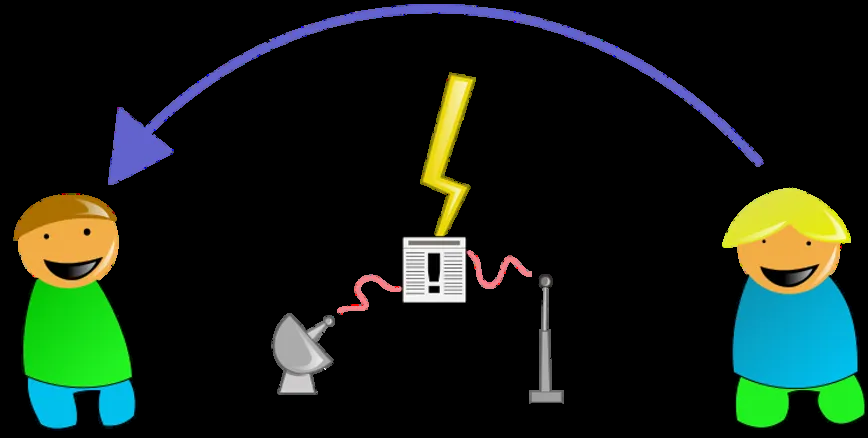
\includegraphics[width=0.9\textwidth]{../assets/ch02/ch02-2_1_数据通信模型-000.png}
    \caption{通信系统一般模型。信源产生的消息经信源编码、信道编码、调制后进入信道传输；接收端经解调、信道译码、信源译码后恢复原始消息。噪声在信道中叠加，是差错的主要来源。}
    \label{fig:comm-model}
\end{figure}

模型的各个部分功能如下：

\textbf{信源（Source）}是消息的产生者。它可以是麦克风（产生模拟语音信号）、摄像头（产生视频流）或键盘（产生数字数据）。从通信系统的角度，信源的输出只有两类：模拟信号和数字信号。

\textbf{信源编码器（Source Encoder）}的任务是压缩：去掉信源输出中的冗余，用尽量少的比特表示信息。ZIP 压缩、JPEG 图像、MP3 音频都是信源编码的例子。没有信源编码，互联网的带宽会在几秒内被耗尽。

\textbf{信道编码器（Channel Encoder）}的任务恰好相反——\textit{增加}冗余。但这些冗余是有结构的，目的是让接收方能从被噪声破坏的信号中恢复出正确的数据。奇偶校验、CRC、汉明码、Turbo 码、LDPC 码都是信道编码的例子。

\textbf{调制器（Modulator）}将数字比特流转换为适合在信道中传输的物理信号。不同的信道需要不同的调制方式：电话线上用 QAM 调制，Wi-Fi 用 OFDM，光纤用 OOK 或 PAM4。

\textbf{信道（Channel）}是传输媒体加上它引入的一切干扰。信道不仅传递信号，也会引入噪声（随机的热噪声）、干扰（其他信号的叠加）和失真（信号波形的畸变）。噪声源在模型中显式标出，提醒我们可靠传输从来不是免费的。

\textbf{接收端}是发送端的镜像：解调器、信道译码器、信源译码器依次恢复出原始消息，最终到达信宿（Sink）——扬声器、屏幕或存储设备。

\subsection{模拟通信与数字通信}

按照信道中传输的信号类型，通信系统分为模拟通信和数字通信。

\textbf{模拟通信}用连续变化的信号（如电压随时间的连续变化）携带信息。传统有线电话就是典型例子：声波推动麦克风膜片振动，转换为连续变化的电流，在铜线上传输，到达接收端再还原为声波。

\textbf{数字通信}用离散的信号（通常是两个电平的序列，即0和1）携带信息。现代通信系统几乎都是数字的。

数字通信为什么能取代模拟通信？根本原因是\textbf{再生中继}。模拟信号每经过一段传输，噪声就会叠加；信号放大时，噪声一并放大，积累下去，质量越来越差。数字信号则不同——接收端不需要精确测量信号的幅度，只需判断它是"高"还是"低"。只要信噪比足够好，接收端就能完美地重建出干净的数字信号，不带任何噪声地继续传递。这就是数字通信的"再生"特性，它让长距离、高质量的通信成为可能。

\begin{figure}[htbp]
    \centering
    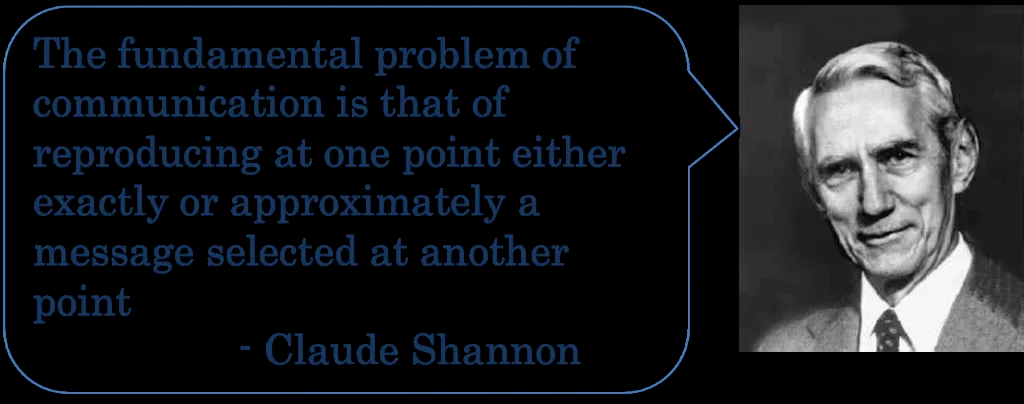
\includegraphics[width=0.85\textwidth]{../assets/ch02/ch02-2_1_数据通信模型-002.png}
    \caption{模拟信号与数字信号的对比。模拟信号（上）幅度连续变化，噪声叠加后无法分离；数字信号（下）只有有限个离散电平，通过阈值判决可以完美再生，噪声不会积累。}
    \label{fig:analog-vs-digital}
\end{figure}

当然，数字通信也有代价：同样的信息，数字化后通常需要更宽的带宽。一路模拟电话只需 4 kHz 带宽，而未压缩的数字电话（PCM）需要 64 kbps，等效于更宽的频带。但随着压缩技术的成熟和光纤带宽的爆发，这一代价已几乎可以忽略。

\subsection{通信方式：单工、半双工与全双工}

点对点通信按数据流向分为三种方式：

\textbf{单工（Simplex）}：数据只能单向流动。广播电台、遥控器是典型例子——发送方永远发，接收方永远收，方向固定。

\textbf{半双工（Half-duplex）}：双方都能收发，但不能同时进行。对讲机是经典案例，说话时按下按钮，释放后才能听到回应。早期的以太网（总线型，CSMA/CD）也是半双工——同一时刻只有一台主机能发送数据。

\textbf{全双工（Full-duplex）}：双方可以同时收发。电话通话是全双工的，你说话的同时对方也能插嘴。现代以太网交换机上的每条链路都是全双工的，消除了冲突，大幅提升了利用率。

\begin{figure}[htbp]
    \centering
    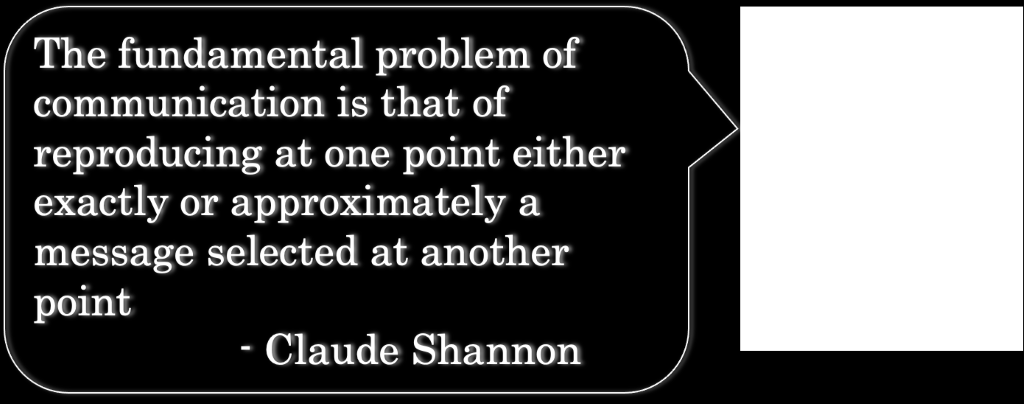
\includegraphics[width=0.8\textwidth]{../assets/ch02/ch02-2_1_数据通信模型-003.png}
    \caption{三种通信方式示意图。(a) 单工；(b) 半双工：同一信道交替使用；(c) 全双工：通常需要两条独立信道（或频分/时分复用的双向信道）。}
    \label{fig:duplex-modes}
\end{figure}

\subsection{数字通信系统模型}

数字通信系统在一般模型的基础上更加明确地展示了各个功能模块：

\begin{figure}[htbp]
    \centering
    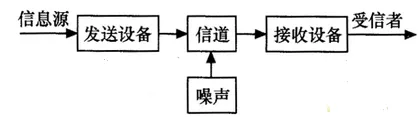
\includegraphics[width=0.95\textwidth]{../assets/ch02/ch02-2_1_数据通信模型-004.png}
    \caption{数字通信系统模型。信源输出经过 A/D 转换（若为模拟信源）、信源编码（压缩）、加密、信道编码（纠错）、数字调制后进入信道；接收端逆向恢复。各模块功能独立，便于单独设计和优化。}
    \label{fig:digital-comm-system}
\end{figure}

值得注意的是\textbf{加密模块}的位置：它在信源编码之后、信道编码之前。这不是随意安排——信源编码后的数据已经被压缩，冗余极少，此时加密效果最好；而信道编码需要在加密后进行，以确保纠错码的保护覆盖加密后的密文（否则信道错误会在解密后产生错误扩散）。

\subsection{从模型到网络}

上述模型描述的是点对点的单向通信。现实中的通信系统是\textbf{网络}——多个节点、多条链路、多种协议交织在一起。点对点的模型是理解网络的基础，但网络带来了新问题：

如何在多个节点之间寻找路径？数据太多时如何排队和调度？多个用户如何共享同一条信道？发生错误或拥塞时如何恢复？这些问题将在后续章节中展开。通信系统一般模型的意义在于：无论网络多复杂，每一条链路、每一个节点上发生的事情，都可以用这个模型来理解。


\chapter{传输媒体}
% 来源: 19c9fb8e-8112-85ce-8000-0000310bad72_2.2_传输媒体.pdf
% 提取时间: 2026-02-28T22:51:31+08:00

2.2 传输媒体
有线传输媒体 or 导向媒体
 双绞线（Twisted Pair）
 同轴电缆（Coaxial Cable）
 光纤（Optical Fiber）
 常用的线缆高速连接模块与接口
  直接连接铜缆 （Direct-Attach Copper, DAC）
  有源光缆（AOC, Active Optical Cable）
无线媒体 or 非导向媒体
 按照频率特性的信号划分

传输媒体是发送器和接收器之间的物理通道， 首先这里给一个具像化的表示，可以看得更清楚一
些




通过电磁波频谱分布特征来看一下对应的应用。电磁波频谱是电磁波按频率或波长划分的范围，广
泛应用于通信、广播、雷达、医疗等领域。电磁波频谱从极低频（ELF）到极高频（EHF）以及更
高频段，每个频段都有其独特的特性和应用。
以几个主要频段为例。
 ● 在极低频（3 Hz ~ 30 Hz）和超低频（30 Hz ~ 300 Hz）具有极强的穿透能力，适合水下和
   地下通信，常用于潜艇通信和地球物理探测。也是话音和乐器所在的频段。
 ● 低频（LF，30 kHz ~ 300 kHz）和中频（MF，300 kHz ~ 3 MHz）主要依靠地面波传播，适
   合长距离广播和导航系统，如AM广播电台。
 ● 高频（HF，3 MHz ~ 30 MHz）利用电离层反射实现远距离通信，广泛应用于短波广播和航空
   通信。
 ● 甚高频（VHF，30 MHz ~ 300 MHz）和特高频（UHF，300 MHz ~ 3 GHz）则以直线传播
   为主，适合电视广播、FM广播、移动通信（如4G）和无线局域网（Wi-Fi）。
 ● 超高频（SHF，3 GHz ~ 30 GHz）和极高频（EHF，30 GHz ~ 300 GHz）具有极高的带宽
   和传输速率，但传播距离较短，主要用于卫星通信、5G网络和雷达系统。
 ● 红外线、可见光、紫外线等光波频段也在自由空间光通信、激光通信和医疗领域有重要应
   用。
上图同样给出了物理媒体的工作区间。根据其特性和应用场景，分为有线传输媒体（双绞线、同轴
电缆、光纤）和无线传输媒体（视距传播、地波、天波）两大类
有线传输媒体 or 导向媒体
双绞线（Twisted Pair）
双绞线是一种常用的有线传输媒体，由两根绝缘的铜导线以螺旋形式绞合在一起组成。这种设计可
以减少电磁干扰（EMI）和串扰，提高信号传输质量。
线缆间串扰：信号通道之间的耦合现象。 双绞线的扭绞结构是为了减少相邻导线之间的串扰和消
除外界干扰
双绞线广泛应用于局域网（LAN）、电话系统和其他短距离通信场景。
结构
 ● 导线：两根绝缘的铜导线。
 ● 绞合方式：两根导线以一定绞距螺旋绞合，以减少外部电磁干扰和线对间的串扰。
 ● 外护套：外层包裹绝缘材料（如PVC）
                    ，用于保护内部导线并提供机械强度。




双绞线
                           网线
双绞线根据是否屏蔽和性能等级分为多种类型：
(1) 非屏蔽双绞线（UTP, Unshielded Twisted Pair）
  ● 无屏蔽层，成本低，易于安装。
  ● 抗干扰能力较弱，适合低噪声环境。
  ● 应用：以太网（如Cat5e、Cat6）    、电话线。
(2) 屏蔽双绞线（STP, Shielded Twisted Pair）
  ● 在绞合线对外增加金属屏蔽层（如铝箔或编织网）              ，抗干扰能力强。
  ● 成本较高，安装复杂。
  ● 应用：工业环境、高噪声场景。
双绞线作为一种常用的传输媒体，具有成本低、易于安装和维护的优点，其绞合设计能有效减少电
磁干扰和串扰，适合短距离通信和局域网部署。然而，双绞线的传输距离有限（通常不超过100
米），带宽较低，且非屏蔽双绞线（UTP）在高噪声环境中的抗干扰能力较弱。尽管如此，双绞线
凭借其经济性和广泛适用性，仍然是许多通信场景中的重要选择。
同轴电缆（Coaxial Cable）
同轴电缆是一种常用的有线传输媒体，由内导体、绝缘层、屏蔽层和外护套组成。其结构设计使其
具有较高的带宽和抗干扰能力，广泛应用于电视广播、网络通信和视频监控等领域。
1. 同轴电缆的结构
  ● 内导体：中心为铜或铝制成的导线，用于传输信号。

  ● 绝缘层：包裹内导体的绝缘材料（如聚乙烯），用于隔离内导体和屏蔽层。
  ● 屏蔽层：金属编织网或铝箔，用于屏蔽外部电磁干扰。
  ● 外护套：最外层的绝缘材料（如PVC）
                     ，用于保护电缆并提供机械强度。




2. 同轴电缆的分类
同轴电缆根据阻抗和用途分为多种类型：
(1) 射频同轴电缆
  ● 阻抗：50Ω或75Ω。

  ● 应用：电视广播、无线电通信、卫星通信。

(2) 视频同轴电缆
  ● 阻抗：75Ω。
  ● 应用：闭路电视（CCTV）
                、视频监控。
(3) 网络同轴电缆
  ● 阻抗：50Ω。
  ● 应用：早期以太网（如10BASE2、10BASE5）
                             。
光纤（Optical Fiber）
光纤是一种利用光信号传输数据的介质，由高纯度的玻璃或塑料制成。由于其高带宽、低损耗和抗
干扰能力强，光纤已成为现代通信网络的核心组成部分，广泛应用于数据中心、电信网络和互联网
骨干网等领域。高锟1966年的论文分析了玻璃纤维损耗大的主要原因，并大胆预言只要能设法降
低玻璃纤维的杂质，就有可能使光纤的损耗从每公里1000dB降低到20dB，从而用于通信。2009
年高锟获得诺贝尔物理学奖。1970年美国康宁公司设计和演示了低损耗18dB/km的光纤。
1. 光纤的结构
光纤通常由以下几层组成：
  ● 纤芯（Core）：中心部分，光信号在此传输。纤芯的直径通常为8～62.5微米。
  ● 包层（Cladding）：包裹纤芯的材料，折射率低于纤芯，用于将光信号限制在纤芯内。
  ● 涂覆层（Coating）：保护光纤的外层，通常由塑料制成，防止机械损伤和环境影响。




2. 光纤的类型
根据传输模式和材料特性，光纤可以分为以下几类：
(1) 单模光纤（Single-Mode Fiber, SMF）单模光纤只允许一种模式的光在其中传播，即基模。
这种模式的光沿着光纤的中心轴线传播，没有模式色散，因此可以实现长距离、高速率的数据传
输，适用于大容量、长距离的通信系统。
  ● 纤芯直径小（通常为8～10微米）        ，只允许一种模式的光信号传输。
  ● 传输距离远（可达数十公里到上百公里）           ，带宽极高。
  ● 成本较高，适合长距离和高带宽应用。

  ● 应用：电信骨干网。数据中心互联（DCI）          。长距离通信（如海底光缆）。
(2) 多模光纤（Multi-Mode Fiber, MMF）多模光纤允许多种模式的光同时在纤芯中传播。不同模
式的光在光纤中传播的路径和速度略有不同，这就会导致模式色散，使得光信号在传输过程中发生
展宽，限制了传输距离和传输速率。多模光纤常用于短距离、低速率的通信系统
  ● 纤芯直径较大（通常为50～62.5微米）        ，允许多种模式的光信号传输。
  ● 传输距离较短（通常为几百米到2公里）          ，带宽较低。
  ● 成本较低，适合短距离和低成本应用。
  ● 应用：局域网（LAN）   。数据中心内部连接。短距离通信（如校园网）。
3.   光纤的工作区




目前光纤通信的主要波长工作区包括：
  ● 850nm： 用于多模光纤，适合短距离通信。
  ● 1310nm： 用于单模光纤，适合中距离通信。

  ● 1550nm： 用于单模光纤，适合长距离通信，支持波分复用技术。

这些波长区域的选择取决于传输距离、带宽需求和成本等因素。随着波分复用技术的发展，光纤的
传输容量和效率将进一步提升，为未来高速通信网络提供强大支持。
4. 光纤的传输原理
光纤利用全反射原理传输光信号：当光从光密介质（折射率较大）射向光疏介质（折射率较小）
时，且入射角大于临界角，就会发生全反射现象。在光纤中，纤芯的折射率高于包层的折射率，光
在纤芯中传播时，遇到纤芯与包层的界面，只要入射角满足条件，光就会在纤芯内不断地发生全反
射，从而沿着光纤向前传播，就像光在光纤内部 “跳跃” 前进一样。
 1. 光信号从纤芯的一端入射。
 2. 由于纤芯的折射率高于包层，光信号在纤芯内不断反射，向前传播。
 3. 光信号最终到达光纤的另一端，完成数据传输。

4. 光纤的优点
 ●  高带宽：支持Tbps级别的传输速率，远超铜缆。
  ● 低损耗：光信号在光纤中传输时衰减极小，适合长距离传输。
  ● 抗干扰能力强：不受电磁干扰，适合高噪声环境。
  ● 安全性高：光信号难以被窃听，数据传输更安全。

  ● 重量轻、体积小：光纤比铜缆更轻便，适合高密度部署。

光纤是否可以弯曲？
光纤在设计和应用中可以弯曲，但其弯曲性能受到严格的物理限制。光纤的弯曲半径必须控制在最
小弯曲半径以内，以避免光信号从纤芯泄漏到包层，导致宏弯损耗或微弯损耗。单模光纤的最小弯
曲半径通常为10倍光纤直径（约1.25毫米），而多模光纤则为20倍光纤直径（约2.5毫米）。过度弯
曲不仅会增加信号衰减，还可能导致光纤断裂，影响传输性能。为了解决这一问题，近年来开发了
弯曲不敏感光纤（Bend-Insensitive Fiber），通过优化纤芯和包层的折射率分布，显著降低了弯曲
损耗，使其在更小的弯曲半径（通常≤5毫米）下仍能保持低损耗和高性能。这种光纤特别适用于
高密度布线、复杂安装环境以及光纤到户（FTTH）等场景。在实际应用中，安装光纤时需严格遵
守最小弯曲半径的要求，并使用保护套管或光纤管理设备来防止外力损伤。定期检查光纤的弯曲状
态也是确保其长期稳定运行的重要措施。总之，光纤的弯曲性能是其设计和部署中需要重点关注的
技术参数，合理的弯曲管理能够有效保障光纤通信系统的高效性和可靠性。
常用的光源有哪些？
常用的光纤通信光源主要包括激光二极管（LD, Laser Diode）和发光二极管（LED, Light
Emitting Diode），它们发射的光波长通常位于光纤的低损耗窗口，如850nm、1310nm和
1550nm。
  ● 激光二极管因其高功率、窄光谱和高速调制特性，成为长距离、高带宽光纤通信的首选光源，
    主要分为分布反馈激光器（DFB Laser）和垂直腔面发射激光器（VCSEL）。DFB激光器发射
    的光波长通常为1310nm或1550nm，具有极高的单色性和稳定性，适用于单模光纤的长距离传
    输，尤其是在电信骨干网和数据中心互联（DCI）中广泛应用；而VCSEL则主要发射850nm波
    长的光，因其低成本、低功耗和高调制速率，广泛用于多模光纤的短距离通信，如数据中心内
    部互联和高性能计算集群。
  ● 发光二极管（LED）虽然成本低且易于制造，但其光谱较宽、调制速率较低，通常发射
    850nm或1310nm波长的光，适用于低速率、短距离的光纤通信系统，如早期的局域网（LAN）
    和光纤到户（FTTH）应用。
此外，随着技术的进步，量子点激光器和外调制激光器等新型光源也逐渐崭露头角，它们通过发射
更稳定的光波长（如1550nm）和提升调制速率，为下一代高速光纤通信系统提供了强有力的支
持。
常用的线缆高速连接模块与接口
SFP（Small Form-factor Pluggable） 是一种小型可插拔的光模块或电模块，广泛用于网络设
备（如交换机、路由器和网卡）中，用于实现光纤或铜缆的连接。
SFP模块的后续版本如下表，这些模块和接口标准推动了数据中心和高性能计算网络的发展，满足
了日益增长的带宽需求。
 类型     速率      通道数       特点         应用
 SFP+ 10Gbps 单通道          体积小，功耗低 10G以太网网络
 SFP28 25Gbps 单通道         支持25G以太网， 25G以太网网络
                          兼容SFP+
 QSFP+ 40Gbps 4通道         支持40G以太网和 40G以太网网络，HPC集群
                （10Gbps/通 InfiniBand
                道）
 QSFP28 100Gbps 4通道       支持100G以太网， 100G以太网网络，数据中心
                （25Gbps/通 兼容QSFP+    骨干网络
                道）
 QSFP56 200Gbp 4通道        支持200G以太网， 200G以太网网络，超大规模
        s       （50Gbps/通 兼容QSFP28   数据中心
                道）
 QSFP- 400Gbp 8通道         支持400G以太网， 400G以太网网络，下一代数
 DD     s       （50Gbps/通 双排引脚设计     据中心互联
                道）
注：SFP28 的单通道速率为28 Gbps，但实际用于25 Gigabit Ethernet（25GbE）时，数据传输
速率为25 Gbps。额外的3 Gbps 用于编码开销（如FEC，前向纠错），以确保数据传输的可靠
性。QSFP-DD 中，“DD” 表示 Double Density（双密度），指的是该光模块的接口设计支持双
排引脚，从而实现了更高的端口密度和传输带宽。QSFP-DD 支持 8 通道，每通道速率可达 50
Gbps（NRZ 调制）或 100 Gbps（PAM4 调制）。总带宽可达 400 Gbps（8x50 Gbps） 或 800
Gbps（8x100 Gbps）。
直接连接铜缆 （Direct-Attach Copper, DAC）
一种用于小型可插拔（SFP）以太网的标准电缆类型，最初定义为SFP+直接连接铜缆
（10GSFP+Cu），它通过有源或无源双轴电缆组件提供10Gbps以太网，并直接连接到SFP+接口。
有源双轴电缆在SFP+接口中包含有源电子元件以改善信号质量；而无源双轴电缆主要是一条直通
的“电线”，几乎不包含任何元件。通常，长度小于7米的双轴电缆是无源的，而长度超过7米的则
是有源的，但这可能因供应商而异。SFP+直接连接铜缆（DAC）因其低延迟和低成本，成为
10Gbps以太网传输距离达10米的流行选择。




结构：
  ● 内部导线：多对双绞线或平行铜线。

  ● 连接器：集成高速连接器（如QSFP+、QSFP28、QSFP-DD）       。
  ● 屏蔽层：通常采用金属屏蔽层减少电磁干扰。

  ● 外护套：柔性外护套，便于布线和安装。

特点：
  ● 无源设计：无需外部电源，功耗低。

  ● 短距离传输：通常支持1米到7米的传输距离。

  ● 高带宽：支持10Gbps、25Gbps、40Gbps、100Gbps甚至400Gbps的传输速率。

应用：
一个主要应用是通过SFP+接口连接网络硬件（数据中心机架内设备互联如服务器到交换机）。这种
连接能够在5米距离内以10Gbps的全双工速度传输数据。此外，这种配置的收发延迟比当前的
10GBASE-T Cat 6/Cat 6A/Cat 7电缆系统低15到25倍：SFP+双轴电缆的延迟为0.1微秒，而
10GBASE-T的延迟为1.5到2.5微秒。SFP+双轴电缆的功耗约为0.1瓦，远低于10GBASE-T的4到8
瓦。
有源光缆（AOC, Active Optical Cable）
有源光缆（AOC）是一种集成光模块的光纤电缆，将光模块的功能直接嵌入电缆两端，提供即插
即用的高速数据传输解决方案。
结构：
 ● 光纤：用于传输光信号。
 ● 光模块：集成在电缆两端，实现电光转换。

 ● 连接器：通常采用高速接口（如QSFP+、QSFP28）   。
 ● AOC的优势：

    ○ 高带宽：支持10Gbps到400Gbps的传输速率。
    ○ 低延迟：光信号传输速度快，延迟极低。

    ○ 轻便灵活：比铜缆更轻，适合高密度部署。

    ○ 即插即用：无需额外配置，安装简便。

 ● AOC的应用场景：
    ○ 数据中心内部互联（如服务器到交换机）     。
    ○ 高性能计算（HPC）和人工智能（AI）集群。

    ○ 短距离高速数据传输（通常≤100米）   。

AOC与DAC的对比
100G DAC & AOC Data Center Cabling Solutions | QSFPTEK
AOC和直接连接铜缆（DAC）都是数据中心常用的高速连接方案，但各有特点：
 特性      AOC（有源光缆）           DAC（直接连接铜缆）
 传输介质    光纤                  铜缆
 传输距离    较长（通常≤100米）         较短（通常≤7米）
 带宽      高（支持10Gbps到400Gbps） 高（支持10Gbps到400Gbps）
 抗干扰能力 强（不受电磁干扰）             较弱（受电磁干扰影响）
 成本      较高                  较低
 应用场景    数据中心内部互联、高性能计算 机架内设备互联
在数据通信和网络设备中，除了高速接口（如SFP、QSFP）之外，还有许多其他常见的接口类
型，例如 RJ45、USB、HDMI 等。这些接口在不同的应用场景中发挥着重要作用。

RJ45 是一种常见的以太网接口，采用8针模块化连接器设计，主要用于连接双绞线电缆（如
Cat5e、Cat6）。它支持从10/100Mbps快速以太网到10Gbps高速以太网的多种速率，传输距离通
常不超过100米。RJ45接口广泛应用于局域网（LAN）、家庭和企业网络以及网络设备（如交换
机、路由器和计算机）的连接，因其成本低、易于安装和广泛兼容性，成为以太网通信中最常用的
接口之一。
RS-232接口有22根线，采用标准的25芯插头座（DB-25）。除此之处，目前广泛应用的还有一种
9芯的RS-232接口（DB-9）。它们的外观都是一个D形的，不过对接的两个接口又分为针式的“公
头”和孔式的“母头”两种，DB-9“母头”和“公头”和DB-25的“母头”和“公头”分别如下图所示
USB（Universal Serial Bus） 是一种通用的串行总线接口，支持数据传输和设备供电。USB接口
有多种版本，包括USB 2.0（480Mbps）、USB 3.0（5Gbps）、USB 3.1（10Gbps）和USB 4
（40Gbps），广泛应用于计算机、外设（如键盘、鼠标、打印机）和移动设备（如智能手机、平
板）的连接，具有即插即用和热插拔的特点。
HDMI（High-Definition Multimedia Interface） 是一种高清多媒体接口，用于传输未压缩的视
频和音频信号。HDMI支持高达48Gbps的传输速率（HDMI 2.1），能够传输4K甚至8K分辨率的内
容，广泛应用于电视、显示器、游戏机和家庭影院系统，提供高质量的视听体验。
光纤接口（如LC、SC） 主要用于光纤通信，支持高带宽和长距离传输。LC接口体积小，适合高
密度部署；SC接口结构稳固，适合数据中心和电信网络。光纤接口广泛应用于数据中心互联、电
信骨干网和高性能计算环境。
无线媒体 or 非导向媒体
美国和中国的频谱划分在管理机制、分配方式和重点频段上存在显著差异。美国通过市场化拍卖和
动态共享机制，推动高频段（如毫米波）的开发；而中国则由国家主导，优先分配中低频段用于
5G建设，并支持行业专网发展。两国的频谱政策都旨在为5G和未来通信技术提供坚实的基础，但
侧重点和实施路径不同。




美国频谱划分                            中国频谱划分
美中频谱划分的对比
 方面     美国                           中国
 管理机构   联邦通信委员会（FCC）                 工业和信息化部（MIIT）
 分配机制   市场化拍卖                        国家统一规划
 5G重点频段 3.5 GHz（CBRS）、28 GHz、39      3.5 GHz、2.6 GHz、4.9 GHz
        GHz
高频段开发  积极推动毫米波（28 GHz、39              逐步推进毫米波（24.75 GHz～27.5
       GHz）                           GHz）
主要频段及应 低频段（<1 GHz）：                   低频段（<1 GHz）：
用       ● 600 MHz：用于5G和广播电             ● 700 MHz：用于5G和广播电视。
          视。                           ● 800 MHz：用于公共安全通信和
        ● 700 MHz：用于公共安全通信               4G LTE。
          和4G LTE。
                                     中频段（1 GHz～6 GHz）：
              中频段（1 GHz～6 GHz）：       ● 2.6 GHz：用于4G LTE和5G。
               ● 2.4 GHz：用于Wi-Fi、蓝牙和  ● 3.5 GHz：用于5G主流频段。
                 物联网（IoT）。            ● 4.9 GHz：用于5G和行业专网。
               ● 3.5 GHz（CBRS）：用于5G和
                 私有网络。
               ● 5 GHz：用于Wi-Fi和5G。
                                     高频段（>6 GHz）：
                                      ● 24.75 GHz～27.5 GHz：用于5G
              高频段（>6 GHz）：              毫米波通信。
               ● 28 GHz和39 GHz：用于5G毫
                                      ● 60 GHz：用于短距离高速通信
                 米波通信。                  （如WiGig）。
               ● 60 GHz：用于WiGig（高速短
                 距离通信）。

按照频率特性的信号划分




1.   地波传播（f < 2 MHz）
地波传播或多或少总沿着地球表面轮廓传播，并且能到达相当远的地方，超出视平线之外。大约在
2MHz以下的频率可以达到这个效果。这个频率内的电磁波之所以会沿着地表曲线传播是由多种因
素造成的。其中之一是电磁波会使地表出现感应电流，其结果是靠近地面的波阵面速度变慢，致使
波阵面向下倾斜，因而会沿着地表曲线传播。另一个因素是衍射，它是一种自然现象，与电磁波遇
到障碍物时的反应有关。在这个频率范围内的电磁波会被大气层散射，以至于它们无法穿透高层大
气。 地波通信广为人知的例子就是调幅无线电广播（AM radio）。
 2. 天波传播 （f < 2 MHz~30MHz）

天波传播用于业余无线电、CB无线电以及国际电台广播，如BBC和美国之音。使用天波传播时，
从基地天线发射出去的信号被高层大气的电离层反射回地球。虽然电波看起来好像被电离层反射，
就如同电离层是坚硬的反射面一样，但实际上这种效果是由折射引起的。稍后我们再来描述折
射。
天波信号可以经过多次反弹传播，在电离层和地球表面之间穿梭几个来回。在这种传播模式下，在
距离发送器几千千米以外的地方也能收到信号。
 3. 视距传播（f > 30MHz）

在高于30MHz的频段上地波和天波传播模式都无法工作，只有视距通信可行。对于卫星通信来
说，高于30MHz的信号不会被电离层反射，因此信号能够在地球站和位于地球站上空且在其视平
线以内的卫星之间传送，对于地面通信，发送天线和接收天线必须在双方有效视距以内。在这里使
用“有效”这个词是因为微波会被大气层弯曲和折射。 在30MHz到1GHz通常称作射频raido区域，
适用于全向通信。1GHz到40GHz叫做微波频率，适用于点对点传输，也用于卫星通信。

\section{[新增-2026-03] 高速光互联技术前沿}

随着AI大模型参数规模从百亿级向万亿级演进，GPU集群内部互联带宽需求持续攀升。448G及更高速率的光互联技术成为支撑下一代AI基础设施的关键技术之一。本节介绍高速光互联的技术要求和前沿发展趋势。

\subsection{448G互联技术背景}

AI大模型训练对网络带宽的需求呈指数级增长：
\begin{itemize}
    \item GPT-3级别模型：百Gbps级互联即可满足
    \item GPT-4级别模型：需要Tbps级互联能力
    \item 未来万亿参数模型：单端口需要448Gbps及以上速率
\end{itemize}

448G互联（即每通道56Gbps PAM4调制 $\times$ 8通道）是下一代高速互联的重要里程碑。

\subsection{448G互联技术要求}

\subsubsection{物理层要求}

\begin{table}[htbp]
\centering
\caption{448G光互联技术指标}
\begin{tabular}{|l|c|c|}
\hline
\textbf{指标} & \textbf{规格} & \textbf{说明} \\
\hline
单通道速率 & 56 Gbps & PAM4调制 \\
\hline
通道数量 & 8通道 & 并行传输 \\
\hline
总带宽 & 448 Gbps & 单向 \\
\hline
调制格式 & PAM4 & 每符号2比特 \\
\hline
信号速率 & 28 GBaud & 波特率 \\
\hline
传输距离 & 100m-2km & 根据应用场景 \\
\hline
误码率 & $<10^{-12}$ & 前向纠错后 \\
\hline
\end{tabular}
\end{table}

\subsubsection{光模块形态}

\textbf{QSFP-DD800}：
\begin{itemize}
    \item 支持8通道 $\times$ 100Gbps PAM4，总带宽800Gbps
    \item 向下兼容QSFP-DD和QSFP28
    \item 功耗控制在15W以内
\end{itemize}

\textbf{OSFP（Octal Small Form-factor Pluggable）}：
\begin{enumerate}
    \item 支持8通道，单通道速率可达112Gbps
    \item 支持液冷散热，适用于高功耗场景
    \item 成为800G/1.6T时代的主流形态
\end{enumerate}

\subsection{关键技术挑战}

\subsubsection{信号完整性挑战}

\begin{enumerate}
    \item \textbf{高频损耗}：56Gbps PAM4信号在PCB上损耗巨大，需采用低损耗材料
    \item \textbf{串扰控制}：高密度引脚间的信号串扰需精确控制
    \item \textbf{阻抗匹配}：全链路阻抗一致性要求极高
\end{enumerate}

\subsubsection{光电器件挑战}

\begin{itemize}
    \item \textbf{激光器带宽}：需要支持28GBaud及以上速率的EML或硅光调制器
    \item \textbf{探测器灵敏度}：高带宽下保持高灵敏度，降低功耗
    \item \textbf{封装散热}：高速器件功耗密度增加，需要先进散热方案
\end{itemize}

\subsubsection{前向纠错（FEC）}

448G互联需要更强的FEC能力：
\begin{enumerate}
    \item 采用级联FEC（CFEC）或拼接FEC（KP4+RS）
    \item 开销控制在10-15\%
    \item 支持AI/ML辅助的信道估计和自适应均衡
\end{enumerate}

\subsection{高速互联架构演进}

\subsubsection{从CPO到NPO}

\textbf{CPO（Co-Packaged Optics，共封装光学）}：
\begin{itemize}
    \item 将光引擎与交换芯片封装在一起
    \item 消除电信号在PCB上的长距离传输
    \item 降低功耗30\%以上，延迟减少50\%
\end{itemize}

\textbf{NPO（Near-Package Optics，近封装光学）}：
\begin{enumerate}
    \item 光引擎靠近交换芯片但独立封装
    \item 平衡性能和可维护性
    \item 有望成为中短期主流方案
\end{enumerate}

\subsubsection{全光交换架构}

\begin{itemize}
    \item 采用OXC实现端口间全光互联
    \item 消除光电转换环节，降低功耗和延迟
    \item 支持灵活的拓扑重配置
\end{itemize}

\subsection{智能高速接口}

\subsubsection{自适应信号处理}

\begin{enumerate}
    \item \textbf{自适应均衡}：根据信道特性自动调整均衡参数
    \item \textbf{动态功耗管理}：根据流量负载调节发射功率
    \item \textbf{温度补偿}：自动补偿温度变化引起的性能漂移
\end{enumerate}

\subsubsection{数字信号处理（DSP）}

\begin{itemize}
    \item 采用先进DSP算法补偿信道损伤
    \item 支持ML-based信道估计和均衡
    \item 实现更长的传输距离和更高的链路裕量
\end{itemize}

\subsubsection{链路诊断与遥测}

\begin{enumerate}
    \item 实时监控链路质量指标（BER、SNR、眼图裕量）
    \item 预测性维护，提前识别潜在故障
    \item 遥测数据用于网络级流量优化
\end{enumerate}

\subsection{技术演进路线图}

\begin{table}[htbp]
\centering
\caption{高速光互联技术演进}
\begin{tabular}{|l|c|c|c|c|}
\hline
\textbf{年代} & \textbf{速率} & \textbf{技术} & \textbf{调制格式} & \textbf{应用场景} \\
\hline
2023-2024 & 400G & QSFP-DD/QSFP112 & PAM4 56Gbps & 当前主流 \\
\hline
2025-2026 & 800G & QSFP-DD800/OSFP & PAM4 112Gbps & 大规模部署 \\
\hline
2027-2028 & 1.6T & CPO/OSFP-XD & PAM4 224Gbps & 下一代超算 \\
\hline
2030+ & 3.2T & 光电融合 & 高阶调制 & 未来演进 \\
\hline
\end{tabular}
\end{table}

高速光互联技术的持续演进为AI大模型训练提供了强大的带宽支撑，CPO/NPO、智能接口等创新技术将进一步提升互联效率和能源利用效率，推动AI基础设施向更高性能、更低功耗的方向发展。

\section{光通信技术：让光为网络插上翅膀}

人类通信的历史，是一部不断追求更快、更远、更大容量信息传递的历史。从古老的狼烟信号到电报、电话，再到现代的光纤通信，每一次技术的飞跃都深刻改变了信息社会的面貌。在众多传输介质中，光——这种我们日常生活中最熟悉的存在——却成为了当今信息时代最关键的传输载体。当我们浏览网页、观看视频、进行视频会议时，你是否想过，这些海量的数据是如何跨越千山万水，精准无误地送达你的屏幕？答案就是光通信技术。光纤通信作为20世纪最伟大的技术发明之一，已经成为现代通信网络的基石。从第一条20dB/km光纤的诞生到如今400G、800G高速光网络的规模部署，光通信技术用半个世纪的时间，重新定义了人类传递信息的方式。在本章中，我们将深入探讨光通信技术的发展脉络、核心技术原理以及未来演进方向，带你理解为什么说“光”才是网络的真正翅膀。

\subsection{光纤通信的诞生：从黑暗走向光明}

要理解光纤通信为什么能够取代传统的铜缆通信，我们首先需要回到20世纪60年代那个充满技术创新的年代。那时的电话网络主要依赖铜缆进行信号传输，随着通话需求的爆炸式增长，工程师们面临着一个严峻的物理瓶颈——铜缆的带宽极限。

让我们先思考一个问题：为什么电信号在金属导线中传输会有容量限制？这要从电磁学的基本原理说起。当高频电信号通过铜缆传输时，会遇到两个主要的物理限制。第一个是趋肤效应，随着信号频率的升高，电流趋向于在导体表面流动，导致有效导电面积减小，电阻增大，信号衰减加剧。第二个是串扰，即相邻导线之间的电磁耦合会引入噪声，限制可传输的信号质量。想象一下，在一根铜缆中同时传输成千上万路电话信号，它们相互干扰，最终能够清晰传递的距离和信号质量都受到严重制约。

在这样的背景下，科学家们开始思考：能否利用光来传输信息？光具有极高的频率——可见光的频率在430THz到750THz之间，这意味着理论上单根光纤可以携带极其庞大的信息量。相比之下，传统无线电波的频率仅为几十GHz到几百GHz，铜缆中的电信号频率更低，差距达到数万倍。然而，把这个理论潜力变为现实，科学家们花了将近十年时间，跨越了无数技术障碍。

1966年，华裔科学家高锟博士发表了一篇具有里程碑意义的论文《光频率介质纤维表面波导》，从理论上论证了利用光纤进行光通信的可能性。高锟指出，制约光通信发展的主要障碍不是光纤本身的损耗，而是当时玻璃材料的纯度不够。他认为，通过改进制造工艺，可以将石英光纤的损耗降低到20dB/km以下，从而实现远距离光通信。这篇论文在当时引起了巨大争议，因为许多科学家认为玻璃的损耗是固有的物理特性，无法克服。但高锟坚持自己的判断，并积极与玻璃制造商合作，推动实际工艺的改进。

1970年，一个值得铭记的年份。康宁玻璃公司（Corning Glass Works）宣布研制成功世界上第一根低损耗光纤，损耗率约为20dB/km，虽然这个数值距离理论极限还有很大距离，但已经足以让光通信成为可能。这一突破与同时期半导体激光器的发明一起，标志着光纤通信时代的正式开启。此后数十年间，光纤的损耗率不断降低，如今商用光纤的损耗约为0.2dB/km，这意味着光信号可以传输超过100公里才衰减到原来的一百分之一。

让我们用一个具体的数字来感受光纤的优越性。一根直径仅125微米（与头发丝相当）的单模光纤，在1550nm波长窗口的损耗为0.2dB/km。假设我们发射一个功率为1毫瓦（0dBm）的光信号，经过100公里传输后，接收端的功率仍有：
\[
P_{out} = P_{in} - \alpha \times L = 0\text{dBm} - 0.2\text{dB/km} \times 100\text{km} = -20\text{dBm}
\]
这相当于10微瓦的功率，在现代光电探测器灵敏度的范围内可以轻松检测到。换成同等传输条件的铜缆，信号早已被噪声淹没，无从辨识。

光纤通信之所以能够取得巨大成功，源于光信号独特的物理优势。首先是极低的损耗，我们已经看到，100公里仅20dB的总衰减意味着光信号可以传输极远的距离，这在跨城、跨省乃至跨洋通信中意味着可以大幅减少中继器的数量，降低系统成本和复杂度。其次是极宽的带宽，单模光纤的理论可用带宽超过10THz，相当于可以同时传输数亿路电话或数百万路高清视频。第三是抗电磁干扰能力，光信号在光纤中传输完全不受外部电磁场影响，因为光是一种电磁波，但它被束缚在光纤内部，不与外界发生电磁耦合。第四是保密性好，传统的铜缆传输会产生电磁辐射，容易被窃听，而光纤中的光信号被完全束缚在纤芯内部，除非物理破坏光纤，否则无法被窃听。最后是体积小、重量轻，一根光缆可以包含数百根光纤，而直径和重量远小于同等容量的铜缆，特别适合空间受限的管道铺设。

正是这些显著优势，使光纤通信在短短半个世纪内从实验室走向全球，从骨干网渗透到接入网，从电信运营商扩展到互联网公司，从传统通信领域进入数据中心。现在，光纤网络已经承载了全球超过90\%的通信流量，成为信息社会名副其实的“神经中枢”。

\subsection{光传输技术的演进：从PDH到OTN}

光纤的发明为光通信提供了物理基础，但要真正实现大容量、远距离的光信号传输，还需要一套完整的光传输技术体系。从上世纪70年代至今，光传输技术经历了多次重大变革，每一代技术都在解决前一代面临的根本性问题。理解这个演进过程，对于把握现代光网络的设计原理至关重要。

让我们首先理解一个核心概念：时分复用（TDM）。在数字通信中，我们要把大量独立的信号合并成一个数据流进行传输，最直观的方法是让这些信号“排队”使用传输通道——每个信号依次占用一小段时间，然后让下一个信号使用。想象一下，一根电话线同时有多人通话，系统会为每个人分配一个固定的时间片，在这个时间片内只有这个人的声音可以通过，时间片结束后切换到下一个人。这种“交替使用”的方式，就是时分复用的本质。在电通信时代，TDM技术被广泛用于提高铜缆的利用率。

准同步数字体系（PDH，Plesiochronous Digital Hierarchy）是最早的光传输技术之一。PDH技术出现于1970年代，它在光纤上传输数字信号，通过时分复用将多个低速信号合并成高速信号流。PDH的基本速率是2.048Mbps（欧洲标准）或1.544Mbps（北美标准），然后通过复用形成更高速率。典型的PDH复用结构是4:1复用，即4个2.048Mbps信号复用成一个8.448Mbps信号，再4个8.448Mbps复用成34.368Mbps，以此类推。

然而，PDH技术存在一个根本性的设计缺陷——时钟同步问题。由于历史原因，不同地区的电信运营商使用不同精度的时钟源，这些时钟虽然标称频率相同，但存在微小的偏差。为了正确分接信号，PDH需要在每个复用层级添加额外的开销比特来补偿时钟差异，这就导致了系统设计的复杂性。更麻烦的是，当我们需要从高速信号中提取某一低速支路信号时，必须将高速信号完全解复用，这种“解复用-再复用”的过程会引入抖动和漂移，影响信号质量。

为了克服PDH的这些缺点，同步数字体系（SDH，Synchronous Digital Hierarchy）应运而生。SDH最初由美国贝尔通信研究所（Bellcore）提出，后来被ITU-T正式标准化为同步数字体系（SDH）和同步光纤网络（SONET）。SDH的核心创新在于引入了同步机制——网络中所有设备都使用同一个高精度时钟源，确保各节点严格同步。这样，SDH可以直接从高速信号中分接出任意低速支路，无需像PDH那样进行繁琐的逐级解复用。

SDH的帧结构是其技术精髓所在。SDH帧是一个结构化的信息块，以STM-1（155.52Mbps）为基本模块，更高速率则由多个STM-1通过字节间插同步复用而成。STM-1帧结构为9行×270列字节，传输周期为125微秒，即每秒传输8000帧，这与PCM语音信号的采样率完美匹配。帧结构中包含了丰富的开销字节，用于网络管理、性能监控、故障定位等功能。特别是段开销（Section Overhead）和通道开销（Path Overhead）的设计，使SDH网络具备了强大的OAM（操作、管理、维护）能力。

SDH技术在1990年代得到了广泛应用，我国的主要运营商都建设了基于SDH的骨干传输网。SDH的环形网络拓扑和自动保护倒换（APS）机制，使其具备了极高的可靠性——当光环网上某处发生故障时，业务可以在50毫秒内自动切换到备用路径，满足了语音通信等实时业务对网络可靠性的严格要求。

然而，随着互联网的爆发式增长，SDH的局限性逐渐显现。SDH是针对传统语音业务设计的，它的带宽分配是刚性的——一旦为某个业务分配了STM-1的带宽，无论该业务是否实际使用这部分带宽，其他业务都无法利用。这种“静态管道”的模式在以IP为代表的突发性数据业务面前显得效率低下。同时，SDH对分组业务的支持能力有限，虽然后来出现了MSTP（Multi-Service Transport Platform，多业务传输平台）来在SDH上承载以太网和IP业务，但这只是权宜之计。

波分复用（WDM，Wavelength Division Multiplexing）技术的出现，为光传输开辟了全新的方向。WDM的原理与无线电通信中的频分复用类似——将不同波长的光信号合并到同一根光纤中传输，在接收端再将它们分开。由于不同波长的光信号彼此独立，可以把它们看作独立的“光通道”，每条通道承载独立的业务。这种“空间换频率”的策略，使单根光纤的容量得到了成倍的提升。

粗波分复用（CWDM，Coarse WDM）是最早的WDM技术，它使用间隔较宽（20nm）的波长通道，典型配置是18个波长通道。由于波长间隔宽，CWDM对激光器的波长精度要求较低，成本相对低廉，但容量有限，主要用于城域网或接入网。

密集波分复用（DWDM，Dense WDM）则将波长间隔压缩到0.4nm甚至更窄，在C波段（1525nm-1565nm）可以同时传输80-160个波长通道，每个波长通道可以承载10Gbps、40Gbps或100Gbps的信号，使单根光纤的总容量达到数Tbps甚至数十Tbps。DWDM技术彻底改变了长距离传输的经济性——原本需要数十条光纤才能承载的流量，现在一条光纤就可以搞定。

然而，DWDM网络也面临新的挑战。在没有电中继的情况下，DWDM信号可以传输的距离受限于光纤损耗和非线性效应。对于100Gbps以上的高速信号，传输距离进一步缩短，需要在每隔80-100公里设置光放大器（如EDFA，Erbium-Doped Fiber Amplifier，掺铒光纤放大器）和色散补偿装置。更重要的是，DWDM系统缺乏像SDH那样的标准化开销机制，网络管理、故障定位、带宽调度等能力都较弱。

光传送网（OTN，Optical Transport Network）正是为了解决这些问题而诞生的。OTN由ITU-T G.709标准定义，它在DWDM的光层之上引入了一个独立的电层处理机制，为波长通道提供了类似SDH的帧结构和开销管理能力。OTN帧的结构称为ODU（Optical Data Unit），从ODU1到ODU4，对应不同的比特速率。ODU4的速率约为100Gbps，与100G DWDM波长通道相匹配。

OTN的核心价值在于提供了一种面向未来的传输架构。它继承了SDH的强大OAM能力——G.709帧结构中包含了丰富的开销字段，用于性能监控、告警指示、故障定位等；同时，它支持波长级的大容量传输，能够充分发挥DWDM技术的带宽潜力。此外，OTN还支持多种客户信号映射（如以太网、SDH、FC等），是一种真正的多业务承载平台。

在OTN架构中，电交叉和光交叉是两种主要的交换机制。电交叉发生在ODU层面，通过电信号处理实现客户信号的复用、解复用和调度，典型设备是OTN交换机或电交叉芯片。光交叉（ROADM，Reconfigurable Optical Add-Drop Multiplexer）则在光层实现波长级别的路由选择——通过波长选择开关（WSS）技术，可以在任意波长端口上下载或穿通任意波长的信号，实现了波长级别的灵活调度。ROADM的出现，使光网络具备了前所未有的灵活性，被认为是下一代智能光网络的核心设备。

近年来，400G DWDM技术开始规模部署。相比100G，400G采用更高级的调制格式（如16QAM或64QAM），在相同的频谱资源下将单波长容量提升了4倍。但高级调制格式对信噪比要求更高，传输距离相应缩短，因此400G系统主要应用于城域和数据中心互联场景。800G和1.6T的研发也已在积极推进中。

\begin{table}[htbp]
\centering
\caption{光传输技术演进对比}
\begin{tabular}{|l|c|c|c|c|}
\hline
\textbf{技术体制} & \textbf{典型速率} & \textbf{复用方式} & \textbf{主要优势} & \textbf{典型应用} \\
\hline
PDH & 2-140Mbps & 时分复用 & 早期标准，简单 & 已被淘汰 \\
\hline
SDH & 155Mbps-10Gbps & 同步时分复用 & 高可靠性，强OAM & 传统骨干网 \\
\hline
WDM/CWDM & 10Gbps×n & 波分复用 & 容量大 & 城域网 \\
\hline
DWDM & 10/40/100Gbps×80+ & 密集波分复用 & 超大容量 & 骨干网/海缆 \\
\hline
OTN & 10/100/400Gbps & 光电复合 & 弹性带宽，智能调度 & 下一代网络 \\
\hline
\end{tabular}
\end{table}

从上表可以看出，光传输技术的演进主线是不断提高单波长速率、增加波长通道数、提升网络灵活性。每一代技术都有其特定的历史使命和应用场景，PDH和SDH为光纤通信的早期发展奠定了基础，WDM/DWDM实现了传输容量的飞跃，OTN则代表了光网络智能化的方向。

\subsection{光纤接入网：从“最后一公里”到全光网络}

前面我们讨论的光传输技术，主要应用在骨干网和城域网层面，承担着城市之间、区域之间的远距离信息传递任务。然而，对于普通用户来说，无论是用手机刷视频还是在家上网，数据的起点和终点往往在用户终端——这就涉及到了接入网的概念。

接入网是通信网络中离用户最近的部分，它负责将用户终端连接到运营商的核心网络。由于直接面向海量用户，接入网的技术选择需要兼顾带宽、覆盖、成本和运维等多个维度。在众多接入技术中，基于光纤的PON（Passive Optical Network，无源光网络）技术已经成为当前主流的宽带接入方案。

让我们首先理解一个基本概念：为什么叫“无源”光网络？传统的电话网络或早期宽带网络，在从运营商机房到用户家庭的这段距离中，往往需要部署大量的有源设备——如放大器、交换机等，这些设备需要供电、维护，成本较高。而PON网络采用无源分光器来实现光信号的分配，这些分光器不需要电源、不需要维护，从而大幅降低了网络建设和运维成本。

一个典型的PON系统由三部分组成：光线路终端（OLT，Optical Line Terminal）位于运营商机房，光网络单元（ONU，Optical Network Unit）位于用户侧，光分配网络（ODN，Optical Distribution Network）连接OLT和ONU。OLT是整个PON系统的核心，负责向上连接城域骨干网，向下管理所有的ONU设备。ONU则安装在用户家中或楼道，提供以太网、Wi-Fi等用户接口。

在典型的树形拓扑中，从OLT发出的光信号经过1:N的分光器后，分发给N个ONU。这里的N通常是8、16、32或64，取决于分光比和传输距离。关键在于，下行方向（从OLT到ONU）的广播式传输——所有ONU都能收到所有数据，但每个ONU只提取属于自己的部分；上行方向（从ONU到OLT）则采用时分多址（TDMA）技术，各个ONU在不同的时间槽中发送数据，避免冲突。

 PON技术经历了从APON、BPON到GPON和EPON的演进。APON（ATM PON）是最早的PON标准，基于ATM协议，但由于ATM协议的复杂性，最终没有获得大规模应用。BPON（Broadband PON）在APON基础上增加了动态带宽分配等特性，但同样未能普及。

GPON（Gigabit PON）和EPON（Ethernet PON）是目前主流的两种PON技术，分别由两个不同的标准化组织主导。GPON由ITU-T G.984系列标准定义，属于国际电信联盟体系，下行速率最高2.5Gbps，上行最高1.25Gbps，支持非对称速率配置。GPON的效率较高——由于采用了GEM（G-PON Encapsulation Mode）封装方式，可以更高效地承载以太网帧和TDM业务。EPON由IEEE 802.3ah标准定义，属于电气电子工程师协会体系，采用以太网帧结构，与现有IP网络天然兼容，部署成本相对较低。这两大标准体系在技术路线上各有侧重：GPON在带宽效率、QoS保障和覆盖距离方面更有优势，而EPON在成本控制和与以太网兼容性方面更具竞争力。我国运营商根据自身网络条件和业务需求，选择了不同的技术路线——中国电信和中国联通主要部署GPON，中国移动则大规模推广EPON，近年来又都向10G-PON演进。

\begin{table}[htbp]
\centering
\caption{主流PON技术对比}
\begin{tabular}{|l|c|c|c|c|}
\hline
\textbf{技术标准} & \textbf{下行速率} & \textbf{上行速率} & \textbf{分光比} & \textbf{主要优势} \\
\hline
EPON & 1Gbps & 1Gbps & 1:32 & 成本低，兼容以太网 \\
\hline
GPON & 2.5Gbps & 1.25Gbps & 1:64 & 效率高，覆盖远 \\
\hline
10G-EPON & 10Gbps & 10Gbps & 1:64 & 带宽提升10倍 \\
\hline
XG(S)-PON & 10Gbps & 2.5Gbps/10Gbps & 1:128 & 超高带宽，下一代主流 \\
\hline
50G-PON & 50Gbps & 25/50Gbps & 1:256 & 面向未来超宽带 \\
\hline
\end{tabular}
\end{table}

10G-PON是PON技术的重大飞跃，它将下行速率提升到10Gbps，是GPON的4倍、EPON的10倍。10G-PON包括XG-PON（非对称，10G/2.5G）和XGS-PON（对称，10G/10G）两种版本。目前，10G-PON正在全球范围内规模部署，我国运营商的用户覆盖已经超过1亿户。

展望未来，50G-PON已被ITU-T标准化，预计将在2025-2030年逐步商用。50G-PON将提供50Gbps的下行速率，足以满足8K视频、AR/VR、云游戏等新兴应用的需求。更重要的是，50G-PON实现了与现有GPON/XGS-PON的共存——可以在同一ODN网络上逐步升级，保护运营商的既有投资。

FTTH（Fiber To The Home，光纤到户）是接入网的终极目标——将光纤直接敷设到用户家庭，用户独享全部带宽资源。我国是全球FTTH部署最领先的国家，根据工信部数据，截至2024年底，我国光纤宽带用户占比已超过95\%，百兆以上宽带用户占比超过90\%，千兆宽带用户数突破2亿。

从技术角度看，FTTH的实现方式包括单星型拓扑和树形拓扑两种。单星型拓扑中，每个用户从OLT直接拉一条专属光纤到户，带宽独享、延迟最低，但光纤资源消耗大，适合高价值商业用户。树形拓扑采用分光器共享光纤资源，建设成本低，是目前主流的FTTH部署模式。

从“最后一公里”到全光网络，光纤接入技术一直在持续演进。回顾这段历史，我们可以看到一个清晰的趋势：带宽越来越宽、距离越来越远、成本越来越低、用户体验越来越好。PON技术以其独特的设计理念——用无源器件替代有源设备——创造了一种极具性价比的宽带接入方案，正在并将持续改变亿万用户的网络体验。值得一提的是，我国是全球FTTH部署最领先的国家，根据工信部数据，截至2024年底，我国光纤宽带用户占比已超过95\%，百兆以上宽带用户占比超过90\%，千兆宽带用户数突破2亿，遥遥领先于其他国家和地区。

\subsection{数据中心光互联：高速网络的核心支撑}

如果说骨干网是通信的“高速公路”，那么数据中心内部网络就是数据的“城市交通网”。随着云计算、大数据和人工智能的快速发展，数据中心已成为现代信息基础设施的核心据点。在这些庞大的计算集群中，成千上万的服务器和存储设备需要高速互联，形成一个高效的信息交换平面。而光互联技术，正是支撑这个平面的关键技术。

让我们首先理解数据中心网络的连接需求。一个典型的数据中心包含数以万计的服务器，它们分布在多个机架（rack）中。每个机架顶部有一台ToR（Top of Rack）交换机，连接机架内所有服务器；ToR交换机再通过上行链路连接到汇聚层交换机；汇聚层交换机进一步连接到核心交换机。这种三级网络架构（接入-汇聚-核心）构成了数据中心网络的经典拓扑。在典型的带宽分配中，接入层（ToR）提供服务器上联带宽，汇聚层承上启下，核心层负责南北向出口，三层的带宽配比通常遵循40\%:20\%:40\%的原则——即ToR上行和核心下行的带宽各占40\%，汇聚层的南北向流量占20\%，这种设计确保各层都不会成为流量瓶颈。

在这些连接中，光模块扮演着至关重要的角色。光模块是实现电信号与光信号相互转换的可插拔器件，它通常包括发射器（激光器+驱动电路）、接收器（探测器+放大电路）和数字诊断功能。根据传输距离和应用场景的不同，光模块可分为多种类型。

短距离光模块主要用于机架内部或相邻机架间的连接，典型传输距离在100米以内。这类场景通常采用多模光纤，850nm波长的垂直腔面发射激光器（VCSEL）是主要的光源方案。多模光纤的优势在于对接精度要求较低，连接器成本低廉，非常适合数据中心内部短距离传输。典型的产品如SFP+（10G）、SFP28（25G）、QSFP28（100G）等。

长距离光模块用于数据中心之间或机架间较长距离的连接，典型传输距离在500米到80公里之间。这类场景主要采用单模光纤，1310nm或1550nm波长的分布反馈（DFB）激光器是主要光源。单模光纤的纤芯直径仅9微米，对接精度要求高，但传输损耗低、色散小，适合远距离传输。

在数据中心网络中，不同距离的连接需要采用不同的光模块技术。让我们以一个具体的例子来说明。假设一个数据中心有1000台服务器，每台服务器配备25G网卡，ToR交换机为48×25G下行+4×100G上行配置。那么服务器到ToR的距离通常在5-30米之间，采用25G AOC（有源光缆）或SFP28光模块；ToR到汇聚交换机的距离可能在100-300米之间，采用100G QSFP28光模块（多模SR4或单模CWDM4/PSM4）；如果汇聚交换机与核心交换机不在同一机房，距离可能达到数公里，就需要采用相干光模块或100G LR4（10公里单模）。

\begin{table}[htbp]
\centering
\caption{数据中心光模块技术对比}
\begin{tabular}{|l|c|c|c|c|c|}
\hline
\textbf{封装形式} & \textbf{速率} & \textbf{光纤类型} & \textbf{典型距离} & \textbf{应用场景} & \textbf{成本} \\
\hline
SFP+ & 10G & 多模/单模 & 300m/10km & 服务器接入 & 低 \\
\hline
SFP28 & 25G & 多模/单模 & 100m/10km & 服务器接入 & 中 \\
\hline
QSFP28 & 100G & 多模SR4 & 100m & ToR互联 & 中 \\
\hline
QSFP28 & 100G & 单模CWDM4 & 2km & 汇聚层 & 中 \\
\hline
QSFP28 & 100G & 单模PSM4 & 500m & 短距离单模 & 中 \\
\hline
QSFP-DD & 400G & 多模/单模 & 100m-10km & 交换机互联 & 高 \\
\hline
OSFP & 400G/800G & 单模 & 2-10km & 核心网络 & 高 \\
\hline
\end{tabular}
\end{table}

400G光模块是当前数据中心网络的主流技术。2019年，400G光模块开始规模部署，主要形态包括QSFP-DD（Double Density）和OSFP。QSFP-DD保持了与QSFP28兼容的尺寸，但通过8×50G的电通道实现400G速率；OSFP（Octal Small Form Factor Pluggable）是新定义的封装标准，尺寸稍大，但支持8×50G通道并预留了更高的功率预算。

在调制技术方面，PAM4（Pulse Amplitude Modulation 4-level，四电平脉冲幅度调制）已成为400G及以上速率的核心技术。相比传统的NRZ（Non-Return-to-Zero）调制，PAM4每个符号周期可以传输2比特信息，使有效数据速率翻倍。以50G PAM4为例，符号率为28Gbaud，但有效数据速率达到56Gbps（28G×2）。这种高效的调制方式使现有电接口和光纤基础设施可以承载更高的比特率。

2024-2025年，800G光模块开始大规模部署。800G采用8×100G PAM4的方案，每个通道使用112Gbaud的PAM4调制。在形态上，800G光模块主要有QSFP-DD800和OSFP两种标准。800G光模块主要用于AI训练集群的交换机互联，以及超大规模数据中心的东西向流量承载。

展望未来，部分厂商预计1.6T光模块将在2026-2027年开始商用。1.6T将采用8×200G或16×100G的方案，更高速率版本可能采用200G波特率的PAM4或更高阶的调制格式。同时，CPO（Co-Packaged Optics，共封装光学）技术正在成为研发热点——将光引擎与交换芯片封装在一起，取代传统的可插拔光模块，可以显著降低功耗和延迟。

对于AI训练集群来说，光互联的重要性更加突出。现代AI训练通常使用数百甚至数千块GPU，这些GPU之间需要频繁交换梯度数据和模型参数。以一个典型的 trillion参数大模型训练任务为例，单次迭代可能产生TB级的通信流量。如果网络延迟过高或带宽不足，GPU将处于等待通信完成的空闲状态，严重影响训练效率。因此，AI训练集群对网络的要求不仅是高带宽，更是超低延迟和确定性时延。

NVLink和InfiniBand已成为AI训练网络的主流技术。NVLink是NVIDIA开发的高速GPU互连技术，通过私有协议实现GPU间的直接通信，延迟可低至微秒级。当NVLink扩展到多GPU服务器之间时，就需要借助InfiniBand网络或基于InfiniBand的NVLink over Fabric。2024年，NVIDIA推出了Spectrum-X以太网平台，专门针对AI训练场景优化，结合了RDMA和自适应路由等技术。

数据中心光互联技术的发展，折射出整个ICT行业的演进趋势：从10G、25G到100G、400G、800G乃至未来的1.6T，速率不断提升；从NRZ到PAM4，调制效率持续优化；从可插拔模块到CPO，封装形态不断创新。每一次技术突破，都推动着数据中心网络向更高性能、更低功耗的方向发展，为云计算、大数据和人工智能提供更强大的基础设施支撑。

\subsection{FIO-IP与OTN跨层互联：打破光与IP的边界}

在现代通信网络中，IP和OTN是两个不同层面的技术——IP相当于通信网络中的“邮政编码系统”，负责确定数据包从源头到目的地的路由路径；OTN则相当于“物流公司的运输网络”，负责实际搬运这些包裹的卡车、飞机和仓库。IP层面关注的是“你的数据要去哪里”，OTN层面关注的是“通过什么路线、用什么方式把数据运过去”。两者需要紧密配合，才能提供端到端的业务服务。这种跨层协同，正是网络架构设计中的一大挑战。

传统的网络设计中，IP层和OTN层相对独立——IP路由器通过高速光接口直连光纤或WDM设备，OTN网络作为透明管道传递IP流量。这种简单直接的连接方式在早期网络中运行良好，但随着网络规模扩大和业务需求复杂化，跨层网络的运维挑战日益凸显。

让我们通过一个具体例子来说明问题。假设某运营商骨干网有多个核心节点，每个节点配置了多台IP路由器和OTN设备，它们之间通过光纤形成复杂的Full Mesh连接。IP层面，这些路由器通过BGP协议形成全互联拓扑，任意两台路由器之间都有业务路径。OTN层面，每条IP链路可能映射到不同的OTN波长或ODU通道，不同的波长可能经过不同的物理路由。

在日常运维中，这样的跨层网络会遇到几个典型问题。第一是电路错连——由于光纤连接错误或标签缺失，本应连接到节点A的光纤被错误地连接到了节点B，导致IP层面的路由计算结果与实际物理连接不符。第二是单点故障——如果OTN层面的两条业务路径恰好使用了相同的光纤或同一个光放大器，一旦该设备故障，将导致IP层面两条独立路径同时中断，失去冗余保护的意义。第三是资源利用率不均——IP层面的负载可能是均衡的，但OTN层面的波长资源可能分布不均，导致部分波长拥塞而其他波长空闲。

为了解决这些问题，业界发展出了多种跨层协同技术。FIO（Fabric Intelligence Orchestrator）是阿里巴巴网络研发团队开发的一套IP-OTN跨层协同系统，它的核心理念是打通IP层和OTN层的信息孤岛，实现跨层拓扑的统一视图和协同优化。

FIO的核心功能包括三个方面。首先是跨层拓扑发现，FIO通过收集IP网络的IGP拓扑信息和OTN网络的GMPLS控制平面信息，构建完整的跨层网络拓扑。在这个拓扑中，每个IP链路可以追溯到其对应的OTN路径，每个OTN波长可以关联到其承载的IP业务。这种端到端的视图是跨层分析的基础。

其次是可靠性分析。在跨层拓扑的基础上，FIO可以分析IP层面的业务路径在OTN层面的物理依赖关系。系统会自动识别“殊途同归”的情况——即IP层面看似冗余的多条路径，在OTN层面实际上共享了相同的物理资源。一旦识别出这种风险，系统会生成整改建议，建议运营商调整OTN层面的波长分配或光缆路由，消除单点故障。

第三是自动化的资源调度。FIO可以根据IP层面的流量预测和业务需求，自动计算OTN层面的波长和时隙分配方案，实现跨层资源的协同优化。这种自动化能力大大减轻了运维人员的工作负担，提高了网络资源利用效率。

FlexE（Flexible Ethernet，灵活以太网）是另一种重要的跨层技术，由OIF（Optical Internetworking Forum）定义。FlexE在传统以太网和OTN之间架起了一座桥梁——它将以太网帧切片映射到OTN的时隙中，实现了以太网业务对OTN带宽的灵活共享。

FlexE的核心概念包括FlexE Group和FlexE Client。一个FlexE Group由多个物理以太网接口组成，这些接口在FlexE层面被捆绑成一个逻辑的高速管道。FlexE Client是映射到FlexE Group中的子速率客户信号，它可以占用Group中特定的时隙，实现带宽的灵活分配——某个FlexE Client可以独享一部分带宽，也可以与其他Client共享带宽。

FlexE的价值在于提供了一种介于以太网和OTN之间的中间层技术。对于需要OTN级别可靠性和端到端管理的大型租户专线业务，FlexE可以提供硬管道隔离，确保业务带宽不被其他流量抢占。同时，FlexE保持了以太网的兼容性，业务无需感知底层传输机制的复杂性。

在5G移动回传网络中，FlexE也发挥着重要作用。5G网络对带宽和时延的要求远高于4G，同时需要支持网络切片。FlexE可以提供基于时隙的硬隔离，为不同类型的5G业务（如eMBB、URLLC、mMTC）提供差异化的传输保障。

G.709 OTN帧结构是OTN技术的核心，它定义了如何将各种客户信号（如以太网、SDH、FC等）封装进OTN帧，以及如何通过丰富的开销字段实现网络管理。OTN帧的基本结构包括帧对齐开销、段开销、通道开销和净荷区域。帧对齐开销用于帧定界和同步；段开销（SOH）负责光传输段层的监控和管理；通道开销（POH）负责端到端的客户信号监控；净荷区域则承载实际的用户数据。

OTN的复用结构采用逐级复用方式：客户信号首先映射进OPU（Optical Payload Unit），OPU再封装进ODU（Optical Data Unit），ODU进一步封装进OTU（Optical Transport Unit）。这种层级化的结构使OTN可以灵活承载从1Gbps到400Gbps的各种业务，同时保持与现有SDH/SONET网络的兼容性。

从FIO到FlexE再到G.709，跨层互联技术的发展反映了网络架构演进的大趋势——打破传统分层架构的边界，构建更加融合、智能的端到端网络能力。在未来，随着网络规模继续扩大、业务需求持续复杂化，跨层协同技术将变得更加重要。

\subsection{光互连技术前沿：从可插拔到光电融合}

经过半个世纪的发展，光通信技术已经取得了巨大的进步。然而，随着数据中心的规模持续扩张、AI训练集群对带宽的需求急剧增长，传统可插拔光模块的局限性日益凸显。功耗、密度、成本——这些挑战推动着光互连技术向新的方向演进。

让我们首先理解可插拔光模块面临的困境。现代数据中心交换机正朝着51.2T乃至更高带宽演进。以51.2T交换机为例，假设采用128×400G的端口配置，需要128个400G光模块。这些光模块的功耗、散热和空间占用都成为系统设计的瓶颈。一个典型的400G QSFP-DD光模块功耗约为10-15W，128个模块的总功耗就超过1kW，加上交换机的功耗，整个系统的散热需求十分惊人。

可插拔光模块的另一个局限是电接口瓶颈。从交换芯片到光模块的电气通道需要驱动56Gbaud甚至112Gbaud的PAM4信号，这些高速信号的传输距离受限于PCB的走线长度和损耗。当光模块数量众多、面板密度很高时，PCB布局和信号完整性设计变得极其困难。

共封装光学（CPO，Co-Packaged Optics）技术正是为了解决这些问题而提出的。CPO的核心理念是将光引擎（Optical Engine）——包括激光器、调制器、探测器等光电器件——与交换芯片（Switch ASIC）集成在同一个封装基板上。这样，光信号在芯片内部产生后，直接通过封装基板上的高速通道传输到光纤接口，消除了传统设计中PCB走线的限制。

CPO技术的优势主要体现在三个方面。第一是降低功耗——由于消除了驱动PCB电容的功耗，CPO可以将光互连的能效提升30\%-50\%。第二是减小延迟——光信号无需经过PCB上的长距离传输，信号延迟可减少50\%以上。第三是提高密度——光引擎与芯片的直接集成，使得在相同面板空间内可以支持更多的光端口。

然而，CPO技术也面临重大挑战。首先是散热问题——交换芯片和光引擎集成在同一封装中，散热设计极其复杂。其次是维护性——CPO模块一旦故障，需要更换整个交换系统模组，不能像可插拔光模块那样热插拔快速修复。第三是供应链——CPO需要光电器件和芯片的深度整合，对供应链整合能力要求很高。

正因为CPO的这些挑战，近封装光学（NPO，Near-Package Optics）作为一种折中方案受到关注。NPO将光引擎放置在交换芯片附近（而不是同一封装中），通过高速柔性电路板（High-Speed Flex）连接。与CPO相比，NPO在散热和维护性方面更加可控，同时仍能获得显著的功耗和延迟改善。

硅光子学（Silicon Photonics）是推动CPO/NPO发展的底层技术。传统光模块使用磷化铟（InP）或砷化镓（GaAs）作为光电器件材料，这些材料与CMOS半导体工艺不兼容，无法实现大规模集成。硅光子学使用成熟的CMOS工艺在硅片上制造光器件，包括硅波导、调制器、探测器等。虽然硅的光电性能不如InP，但硅光子技术的最大优势是能够利用成熟的半导体制造工艺，实现光电器件与控制电路的单片集成，大幅降低成本和尺寸。

硅光子在数据中心光模块中已经开始应用。Intel、Broadcom等公司已推出基于硅光子的100G、400G光模块产品。硅光子的集成优势使其在高速率（400G及以上）场景更具竞争力，预计到2028年，硅光子光模块的市场份额将超过50\%。

光电路交换（OCS，Optical Circuit Switch）代表了另一种光网络创新方向。传统的电交换需要将光信号转换为电信号进行处理，消耗大量功耗和时延。OCS在光层实现端口间的直连切换，数据始终以光的形式传输，无需光电转换。OCS特别适合需要频繁改变网络拓扑的数据中心场景，可以显著提高网络灵活性和能效。

阿里云在光互连领域的实践值得关注。从2015年开始，阿里巴巴启动了光模块自研项目，逐步掌握了光模块的设计和制造能力。目前，阿里巴巴的数据中心已部署了数百万只自研光模块，覆盖了从10G到400G的全系列 产品。通过光模块自研，阿里巴巴不仅显著降低了采购成本，更重要的是摆脱了对单一设备厂商的依赖，掌握了技术演进的主导权。在400G时代，阿里主导成立了SFP-DD MSA和QSFP112 MSA标准组织，联合上下游厂商共同制定技术规范，推动了行业技术标准的统一。目前，阿里巴巴正在积极布局800G/1.6T光模块、硅光子技术和CPO共封装光学，目标是实现从光芯片到光模块的全链路自主可控。根据公开信息，阿里巴巴已累计出货超过100万只自研光模块，成为全球光模块用量最大的互联网公司之一。

展望未来，光互连技术的发展将呈现几个明确趋势。第一是带宽持续提升——从400G到800G再到1.6T，单端口速率将继续翻倍增长。第二是光电融合加深——从可插拔到CPO/NPO再到完全光电集成，集成度不断提高。第三是智能化——光网络将具备更强的状态感知、故障预测和自适应调整能力。第四是绿色化——随着“双碳”目标的推进，降低功耗将成为光互连技术的核心追求。

\begin{table}[htbp]
\centering
\caption{光互连技术演进路线}
\begin{tabular}{|l|c|c|c|c|}
\hline
\textbf{技术阶段} & \textbf{时间节点} & \textbf{典型速率} & \textbf{核心特点} & \textbf{应用场景} \\
\hline
可插拔模块 & 2015-2024 & 100G-400G & 标准化的模块化产品 & 当前主流部署 \\
\hline
QSFP-DD800 & 2024-2025 & 800G & PAM4 112G SerDes & AI训练集群 \\
\hline
OSFP-XD & 2026-2027 & 800G-1.6T & 更高功率预算 & 下一代数据中心 \\
\hline
NPO & 2025-2027 & 1.6T-3.2T & 光引擎靠近芯片 & 过渡方案 \\
\hline
CPO & 2027+ & 3.2T+ & 光电同封，极致能效 & 超大规模集群 \\
\hline
\end{tabular}
\end{table}

光通信技术之所以能不断发展创新，根本动力来自于人类对更高速率、更大容量、更低延迟通信的永恒追求。从第一根低损耗光纤诞生到如今，CMOS硅光子集成、智能光网络等创新技术正在重塑光通信的形态。可以预见，在未来相当长的时期内，光仍将是网络世界最重要的信息载体，光通信技术将继续沿着更高性能、更低功耗、更智能的方向演进。

\subsection{本章小结}

光通信技术是现代信息社会的基础设施，从光纤通信的诞生到如今多元化应用，已经走过了半个多世纪的历程。在本章中，我们系统地探讨了光通信技术的发展脉络、核心技术原理和未来演进方向。

首先，我们回顾了光纤通信的诞生历程。从1966年高锟博士提出光纤通信的理论可能性，到1970年康宁公司研制成功20dB/km低损耗光纤，光纤通信经历了从理论到实践的关键突破。光信号相比电信号具有损耗低、带宽宽、抗电磁干扰、保密性好等独特优势，使其成为当代通信网络的理想传输介质。

其次，我们梳理了光传输技术的演进路线。从PDH到SDH，从WDM到DWDM再到OTN，每一代技术都解决了前一代的核心痛点。PDH/SDH实现了光纤上的数字化传输，WDM/DWDM大幅提升了单根光纤的传输容量，OTN则在光层之上引入了类似SDH的帧结构和开销管理能力，实现了光网络的智能化。

在接入网领域，PON技术以其“无源”的独特设计理念，成为光纤到户的主流方案。从GPON/EPON到10G-PON再到未来的50G-PON，PON技术持续演进，为亿万用户提供了越来越宽带的网络接入体验。

数据中心光互联是近年来发展最快的领域之一。400G光模块已规模部署，800G光模块正在大规模商用，1.6T光模块和CPO技术也在积极推进中。AI训练等新兴应用对网络带宽和延迟提出了更高要求，推动着光互联技术不断突破极限。

跨层互联技术（FIO、FlexE、G.709 OTN）打通了IP层和OTN层的信息孤岛，实现了端到端的网络视图和协同优化。随着网络规模扩大和业务需求复杂化，跨层协同将成为网络架构设计的重要方向。

最后，光互连技术正朝着光电融合的方向演进。CPO/NPO技术将光引擎与交换芯片集成，可大幅降低功耗和延迟；硅光子技术为光电集成提供了CMOS兼容的工艺平台；光电路交换（OCS）实现了纯光层面的网络切换。这些前沿技术创新，将推动光通信进入新的发展阶段。

光通信技术不仅仅是通信工程师的专业领域，它已经渗透到我们日常生活的方方面面。当我们刷视频、逛网购、玩云游戏时，光纤正在以光速传递着每一个比特的信息。未来，随着AI、元宇宙、量子通信等新技术的发展，光通信将面临新的机遇与挑战。但无论如何演进，“让光为网络插上翅膀”这一核心理念将始终指引着光通信技术的发展方向。


\chapter{信号}
\section{信号与无线信道}

\subsection{信号的本质}

我们每天都在与信号打交道。当你说话时，声波在空气中传播；当你打开手机，电磁波在空间中穿行。但这两种信号有着本质的区别。

声波是纵波，它的振动方向与传播方向相同，依靠空气分子的疏密变化来传递能量。这也是为什么声波无法在真空中传播——没有介质，就没有可以振动的分子。但电磁波不同，它是横波，电场与磁场的振动方向都与传播方向垂直，且互相垂直。这种结构使电磁波可以在真空中传播，速度达到每秒30万公里，远超声波在空气中的344米每秒。

\begin{figure}[htbp]
    \centering
    
\includegraphics[width=0.7\textwidth]{assets/ch02/ch02-2_3_信号-000.png}
    \caption{纵波（P波）传播示意图：质点振动方向与波传播方向相同}
    \label{fig:p-wave}
\end{figure}

这一物理特性决定了无线通信的可能。但自由传播的代价是信道环境的不可控性——与封闭的导线不同，无线信号要穿越开放空间，遭遇各种障碍和干扰。理解这些特性，是设计无线通信系统的起点。

\subsection{正弦波与信号的基本参数}

最简单的信号是正弦波。虽然它看似简单，但任何复杂的周期信号都可以分解为正弦波的叠加。正弦波的数学表达式为
\begin{equation}
    s(t) = A \sin(2\pi f t + \phi)
\end{equation}
其中 $A$ 是振幅，表示信号的强度；$f$ 是频率，单位为赫兹（Hz），表示每秒振动的次数；$\phi$ 是相位，表示信号在时间轴上的起始位置。周期 $T$ 与频率互为倒数，$T = 1/f$；波长 $\lambda$ 则是一个周期占据的空间长度，$\lambda = vT$，其中 $v$ 是传播速度。

\begin{figure}[htbp]
    \centering
    
\includegraphics[width=0.9\textwidth]{assets/ch02/ch02-2_3_信号-003.png}
    \caption{正弦波的参数变化：振幅、频率和相位对波形的影响}
    \label{fig:sine-parameters}
\end{figure}

振幅与频率的物理意义直观可感。弹吉他时，用力拨弦会增大振幅，声音更响亮；使用更细的弦会提高振动频率，音调更高。人耳可感知的声波频率范围约为20 Hz到20 kHz。电话系统为了节省带宽，通常只传输300到3400 Hz的范围；高保真音响则追求20 Hz到20 kHz的全频带还原。

\subsection{傅里叶分析：从时域到频域}

实际通信中的信号远比正弦波复杂。但1768年出生的法国数学家傅里叶发现，任何周期信号都可以表示为正弦波的和。这一发现成为信号分析的基石。

考虑一个周期为 $T$ 的信号 $s(t)$，满足 $s(t) = s(t+T)$。傅里叶证明了，这个信号可以写成
\begin{equation}
    s(t) = a_0 + \sum_{n=1}^{\infty} \left( a_n \cos \frac{2\pi n t}{T} + b_n \sin \frac{2\pi n t}{T} \right)
\end{equation}
这就是傅里叶级数。其中 $a_0$ 是直流分量，$n=1$ 的项是基频分量，$n>1$ 的项是谐波分量。

\begin{figure}[htbp]
    \centering
    
\includegraphics[width=0.6\textwidth]{assets/ch02/ch02-2_3_信号-009.png}
    \caption{周期信号的傅里叶级数展开：任意周期信号可表示为正弦/余弦波的叠加}
    \label{fig:fourier-series}
\end{figure}

现在的问题是：如何确定这些系数 $a_n$ 和 $b_n$？

\subsubsection{正交性的核心作用}

求解系数的关键在于三角函数的\textbf{正交性}。正交原本是几何概念，指两个矢量成直角。函数的正交性与此类似：如果两个函数在一个周期内的乘积积分为零，就称它们正交。

正弦和余弦函数具有优美的正交性质。在 $[0, 2\pi]$ 区间内，$\sin x$ 与 $\cos x$ 正交，因为它们相差 $\pi/2$ 的相位——在圆周上正好是90度。更一般地，不同频率的正弦函数互相正交，相同频率的正弦和余弦也正交。

\begin{figure}[htbp]
    \centering
    
\includegraphics[width=0.5\textwidth]{assets/ch02/ch02-2_3_信号-013.png}
    \caption{三角函数积化和差公式：用于验证正交性关系}
    \label{fig:trig-formulas}
\end{figure}

具体而言，对于整数 $m, n$：
\begin{align}
    \int_0^{2\pi} \sin(mx) \cos(nx) \, dx &= 0 \quad \text{（对所有 $m, n$）} \\
    \int_0^{2\pi} \sin(mx) \sin(nx) \, dx &= \begin{cases} \pi, & m = n \neq 0 \\ 0, & m \neq n \end{cases} \\
    \int_0^{2\pi} \cos(mx) \cos(nx) \, dx &= \begin{cases} \pi, & m = n \neq 0 \\ 2\pi, & m = n = 0 \\ 0, & m \neq n \end{cases}
\end{align}

这些等式可以通过三角函数的积化和差公式证明，但它们的意义更为深远：正交性使我们能够"提取"信号中特定频率的成分。

\subsubsection{系数求解的推导}

利用正交性，我们可以逐一确定傅里叶系数。以求 $b_n$（正弦分量的系数）为例，将傅里叶级数两边乘以 $\sin(nx)$ 并在 $[0, 2\pi]$ 上积分：
\begin{equation}
    \int_0^{2\pi} s(x) \sin(nx) \, dx = \int_0^{2\pi} \left[ a_0 + \sum_{m=1}^{\infty} (a_m \cos(mx) + b_m \sin(mx)) \right] \sin(nx) \, dx
\end{equation}

根据正交性，右边只剩下 $m=n$ 的正弦项：
\begin{equation}
    \int_0^{2\pi} s(x) \sin(nx) \, dx = b_n \int_0^{2\pi} \sin^2(nx) \, dx = b_n \cdot \pi
\end{equation}

因此
\begin{equation}
    b_n = \frac{1}{\pi} \int_0^{2\pi} s(x) \sin(nx) \, dx
\end{equation}

同理，对于余弦系数：
\begin{equation}
    a_n = \frac{1}{\pi} \int_0^{2\pi} s(x) \cos(nx) \, dx \quad (n \geq 1)
\end{equation}

直流分量 $a_0$ 稍有不同，因为 $\cos(0) = 1$ 的积分范数是 $2\pi$：
\begin{equation}
    a_0 = \frac{1}{2\pi} \int_0^{2\pi} s(x) \, dx
\end{equation}

这就是傅里叶系数的完整表达式。它们告诉我们：任何周期信号都由一个直流分量和一系列正弦、余弦谐波组成，各分量的强度由上述积分确定。

\subsubsection{指数形式的统一表达}

傅里叶级数还可以写成更紧凑的指数形式。利用欧拉公式 $e^{j\theta} = \cos\theta + j\sin\theta$，可以验证三角级数与指数级数的等价性。

定义复系数
\begin{equation}
    c_n = \frac{1}{2\pi} \int_0^{2\pi} s(x) e^{-jnx} \, dx
\end{equation}

则信号表示为
\begin{equation}
    s(t) = \sum_{n=-\infty}^{\infty} c_n e^{jnt}
\end{equation}

这种形式在计算上更为简洁，也便于推广到非周期信号的傅里叶变换。

\begin{figure}[htbp]
    \centering
    
\includegraphics[width=0.9\textwidth]{assets/ch02/ch02-2_3_信号-028.png}
    \caption{五种傅里叶变换形式的对照表：时域与频域特性的对应关系}
    \label{fig:fourier-transforms}
\end{figure}

\subsection{信号的能量与功率}

信号的能量和功率是衡量信号强度的基本指标。能量定义为信号平方的积分
\begin{equation}
    E = \int_{-\infty}^{\infty} |x(t)|^2 dt
\end{equation}

对于周期信号，能量无限，因此定义平均功率更有意义
\begin{equation}
    P = \frac{1}{T_0} \int_0^{T_0} |x(t)|^2 dt
\end{equation}

这里有一个深刻的结果。将周期信号的傅里叶级数代入功率表达式，利用正交性，得到
\begin{equation}
    P = |a_0|^2 + \frac{1}{2} \sum_{n=1}^{\infty} (|a_n|^2 + |b_n|^2) = \sum_{n=-\infty}^{\infty} |c_n|^2
\end{equation}

这就是\textbf{帕塞瓦尔定理}：信号的时域功率等于其各频率分量功率之和。它表明能量在时域和频域的分布是等价的。

\begin{figure}[htbp]
    \centering
    
\includegraphics[width=0.4\textwidth]{assets/ch02/ch02-2_3_信号-032.png}
    \caption{功率谱密度定义：信号功率在频域的分布}
    \label{fig:psd}
\end{figure}

\subsection{无线信道的挑战}

有线通信中，信号被限制在导线内，环境相对可控。无线通信面对的是开放空间，信号在传播过程中遭遇多种损伤。

\subsubsection{路径损耗与距离的较量}

最基本的损伤是路径损耗——信号随距离增加而衰减。自由空间模型给出了理论基准
\begin{equation}
    P_r = P_t \cdot G_t \cdot G_r \cdot \left(\frac{\lambda}{4\pi d}\right)^2
\end{equation}

其中 $P_t$ 和 $P_r$ 分别是发射和接收功率，$G_t$ 和 $G_r$ 是天线增益，$\lambda$ 是波长，$d$ 是距离。这个公式揭示了两个重要事实：接收功率与距离的平方成反比，与波长的平方成正比。高频信号（短波长）比低频信号衰减更快。

但真实环境远比自由空间复杂。城市中的建筑物、山丘、植被都会阻挡信号。这种阻挡是随机的——你无法精确预测某一具体位置的遮挡程度，但可以用统计模型描述。研究者发现，考虑这些障碍物的综合效应后，信号衰减服从对数正态分布。对数距离路径损耗模型将确定性衰减和随机阴影结合
\begin{equation}
    PL(d) = PL(d_0) + 10n \log_{10}\left(\frac{d}{d_0}\right) + X_\sigma
\end{equation}
其中 $n$ 是路径损耗指数，自由空间 $n=2$，城市环境可达 $3.7$ 到 $6.5$；$X_\sigma$ 是零均值高斯随机变量，代表阴影衰落的随机性。

\subsubsection{多径效应与小尺度衰落}

比阴影更复杂的是多径效应。无线信号从发射端到接收端，可能经历反射、折射、散射和绕射，通过多条路径到达。这些路径长度不同，信号副本以不同相位叠加，导致接收信号强度的快速波动。

多径信道可以用时变冲激响应描述
\begin{equation}
    h(t, \tau) = \sum_{i=1}^{N(t)} a_i(t) e^{-j\phi_i(t)} \delta(\tau - \tau_i(t))
\end{equation}
其中 $a_i$ 是第 $i$ 条路径的幅度，$\tau_i$ 是时延，$\phi_i$ 是相位，$N$ 是多径数量。

由此引出几个关键参数。时延扩展 $T_m$ 是最大多径时延差，它决定了信道是否频率选择性——如果信号带宽远大于 $1/T_m$，不同频率会经历不同衰落。相干带宽 $B_c \approx 1/T_m$ 是信道响应近似恒定的频率范围。

类似地，移动导致的多普勒效应使信道随时间变化。多普勒扩展 $f_D = v/\lambda$ 衡量这种变化的速度，相干时间 $T_c \approx 1/f_D$ 是信道近似不变的时间窗口。

\subsubsection{衰落的统计模型}

当没有直射路径且多径丰富时，接收信号包络服从\textbf{瑞利分布}
\begin{equation}
    f_R(r) = \frac{r}{\sigma^2} e^{-r^2/(2\sigma^2)}, \quad r \geq 0
\end{equation}
这是大量独立多径分量的矢量和的结果。根据中心极限定理，同相和正交分量都服从高斯分布，其包络即为瑞利分布。

当存在直射路径时，信号包含一个稳定分量叠加随机多径，此时包络服从\textbf{莱斯分布}
\begin{equation}
    f_R(r) = \frac{r}{\sigma^2} e^{-(r^2+K^2)/(2\sigma^2)} I_0\left(\frac{rK}{\sigma^2}\right)
\end{equation}
其中 $K$ 是莱斯因子，表示直射分量与散射分量的功率比。$K$ 越大，信道越稳定，越接近AWGN信道；$K$ 越小，越接近瑞利衰落。

\subsubsection{噪声的物理起源}

无线信道中不可避免的干扰是噪声。热噪声源于导体中电子的热运动，其功率谱密度为 $N_0 = kT$，其中 $k$ 是玻尔兹曼常数，$T$ 是绝对温度。在带宽 $B$ 内的噪声功率为 $N = kTB$。

热噪声被建模为\textbf{加性高斯白噪声}（AWGN）。"加性"表示噪声独立叠加于信号；"高斯"表示幅度服从高斯分布；"白"表示功率谱密度在所有频率上为常数。AWGN是通信系统分析的标准模型，实际系统的性能最终都受限于这一物理噪声。

信噪比 $\text{SNR} = S/N$ 是信号功率与噪声功率之比，是决定通信质量的关键参数。提高发射功率可以增加SNR，但受限于法规和设备能力；降低噪声需要更先进的低噪声放大器或更冷的接收机——后者在深空通信中确实被采用。

\subsection{从傅里叶到拉普拉斯：为什么要推广}

傅里叶分析提供了观察信号的频域视角，但它有一个根本性的限制——要求信号满足绝对可积条件。许多实际信号并不满足这一条件：阶跃信号在无穷远处不衰减，指数增长的信号能量无限，这些信号在严格意义上没有傅里叶变换。

更重要的是，傅里叶变换无法直接处理系统的因果性。当我们分析一个从某一时刻启动的电路，或研究一个从静止开始运动的机械系统，初始条件如何纳入分析框架？系统的瞬态响应如何与稳态特性统一描述？

拉普拉斯变换正是为解决这些问题而生。它通过引入一个指数衰减因子 $e^{-\sigma t}$，将原本不收敛的信号转化为可变换的形式，同时将微分方程转化为代数方程，将初始条件自然地嵌入变换域。

\subsubsection{收敛性与衰减因子}

考虑一个简单的问题：单位阶跃信号 $u(t)$ 在 $t \geq 0$ 时恒为1，它的傅里叶变换存在吗？从定义出发
\begin{equation}
    \int_{-\infty}^{\infty} u(t) e^{-j\omega t} dt = \int_{0}^{\infty} e^{-j\omega t} dt
\end{equation}
这个积分不收敛，因为被积函数在 $t \to \infty$ 时不趋于零。但如果我们乘以一个衰减因子 $e^{-\sigma t}$，其中 $\sigma > 0$
\begin{equation}
    \int_{0}^{\infty} e^{-\sigma t} e^{-j\omega t} dt = \int_{0}^{\infty} e^{-(\sigma + j\omega)t} dt = \frac{1}{\sigma + j\omega}
\end{equation}
积分收敛了。这个观察引向关键的推广：将频率从实轴扩展到复平面。

定义复频率 $s = \sigma + j\omega$，其中 $\sigma$ 是实部，控制衰减或增长；$\omega$ 是虚部，代表角频率。信号 $x(t)$ 的双边拉普拉斯变换定义为
\begin{equation}
    X(s) = \int_{-\infty}^{\infty} x(t) e^{-st} dt
\end{equation}

当 $\sigma = 0$ 时，$s = j\omega$，拉普拉斯变换退化为傅里叶变换。这意味着傅里叶变换是拉普拉斯变换在虚轴上的特例。拉普拉斯变换将频域分析推广到整个复平面，大大扩展了可分析信号的范围。

\subsubsection{单边变换与因果系统}

实际系统通常是因果的——响应不会早于激励发生。对于因果信号 $x(t) = 0$（当 $t < 0$），单边拉普拉斯变换更为适用
\begin{equation}
    X(s) = \int_{0^-}^{\infty} x(t) e^{-st} dt
\end{equation}
积分下限 $0^-$ 包含了 $t=0$ 时刻可能存在的冲激，确保初始条件被完整捕获。

单边变换的真正威力体现在微分性质上。考虑 $x(t)$ 的导数的变换
\begin{equation}
    \mathcal{L}\left\{\frac{dx}{dt}\right\} = \int_{0^-}^{\infty} \frac{dx}{dt} e^{-st} dt
\end{equation}
分部积分得到
\begin{equation}
    \mathcal{L}\left\{\frac{dx}{dt}\right\} = sX(s) - x(0^-)
\end{equation}
导数运算变成了乘以 $s$ 并减去初始值。这一性质将时域微分方程转化为变换域的代数方程，初始条件 $x(0^-)$ 自然地出现在方程中。

\subsubsection{系统分析与传递函数}

线性时不变系统由冲激响应 $h(t)$ 完全刻画。输入 $x(t)$ 产生的输出是卷积 $y(t) = x(t) * h(t)$。在拉普拉斯域，卷积变为乘积
\begin{equation}
    Y(s) = X(s) H(s)
\end{equation}
其中 $H(s)$ 是系统的传递函数，是冲激响应的拉普拉斯变换。

传递函数提供了系统分析的强大工具。系统的极点（使 $H(s)$ 分母为零的 $s$ 值）决定了系统的固有响应模式。实极点对应指数衰减或增长，共轭复极点对应衰减或增长的正弦振荡。极点的位置揭示了系统的稳定性：所有极点位于左半平面时，系统稳定；存在右半平面极点时，系统不稳定。

零点（使 $H(s)$ 分子为零的 $s$ 值）则影响系统的频率选择特性。极零点在复平面上的配置完全刻画了系统的输入输出行为，这是控制系统设计的几何语言。

\subsubsection{从连续到离散：Z变换的引入}

数字信号处理将连续时间信号采样为离散序列。采样间隔 $T$ 将连续时间 $t$ 映射为离散序号 $n$，信号 $x(t)$ 变为序列 $x[n] = x(nT)$。

对离散序列直接应用拉普拉斯变换，令 $t = nT$
\begin{equation}
    X(s) = \sum_{n=-\infty}^{\infty} x[n] e^{-snT}
\end{equation}
定义 $z = e^{sT}$，则 $e^{-snT} = z^{-n}$，得到Z变换的定义
\begin{equation}
    X(z) = \sum_{n=-\infty}^{\infty} x[n] z^{-n}
\end{equation}

Z变换与拉普拉斯变换通过 $z = e^{sT}$ 关联。复 $s$ 平面的虚轴映射到 $z$ 平面的单位圆，左半平面映射到单位圆内部，右半平面映射到单位圆外部。稳定系统的极点必须位于单位圆内。

\subsubsection{Z变换的性质与系统分析}

Z变换继承了拉普拉斯变换的核心优点，并适应了离散时间特性。时移性质尤为简洁：序列右移一位对应乘以 $z^{-1}$
\begin{equation}
    \mathcal{Z}\{x[n-1]\} = z^{-1} X(z)
\end{equation}
$z^{-1}$ 因此被称为单位延迟算子，它是数字滤波器实现的基本构件。

差分方程描述离散时间系统，类似于连续时间的微分方程。Z变换将差分方程转化为代数方程。考虑一阶差分方程
\begin{equation}
    y[n] + a y[n-1] = b x[n]
\end{equation}
Z变换后得到
\begin{equation}
    Y(z) + a z^{-1} Y(z) = b X(z)
\end{equation}
传递函数为
\begin{equation}
    H(z) = \frac{Y(z)}{X(z)} = \frac{b}{1 + a z^{-1}} = \frac{b z}{z + a}
\end{equation}
极点位于 $z = -a$。当 $|a| < 1$ 时极点在单位圆内，系统稳定。这一判据比连续时间系统更直观——只需检查极点是否在单位圆内。

\subsubsection{三种变换的统一视角}

傅里叶变换、拉普拉斯变换和Z变换构成了信号分析的三层框架。傅里叶变换分析信号的频谱组成，适用于稳态、能量有限的信号。拉普拉斯变换扩展了分析范围，引入衰减因子处理增长信号，自然纳入初始条件，统一描述瞬态和稳态响应。Z变换将这一框架移植到离散时间领域，为数字信号处理提供数学基础。

三者的关系通过极限和映射体现。拉普拉斯变换在虚轴上退化为傅里叶变换；Z变换通过 $z = e^{sT}$ 与拉普拉斯变换关联，当采样间隔 $T \to 0$ 时，Z变换趋近拉普拉斯变换。这一层次结构使工程师能够在不同域中选择最适合的分析工具，而它们之间的深刻联系确保了理论的一致性和完整性。

在通信系统设计中，这些变换各有用武之地。模拟滤波器设计在拉普拉斯域进行，通过极零点配置实现所需的频率响应。数字滤波器在Z域设计，通过差分方程实现。系统级仿真则在频域进行，利用傅里叶变换的快速算法计算信号通过线性系统的响应。掌握这三种变换及其相互关系，是深入理解信号处理与通信系统的关键。


\chapter{数字信号编码}
\section{数字信号编码}

\subsection{为什么需要编码}

数字通信系统处理的是0和1组成的序列，但这些二进制数据不能直接在物理信道上传输。原始的二进制流往往包含长串的0或1，这会带来三个问题。

首先，频谱可能不适合信道特性。许多信道（如变压器耦合的线路）无法传输直流分量，而原始二进制流可能有偏（0和1数量不等），导致直流偏移。其次，接收端需要从接收信号中提取时钟以确定抽样时刻。如果流中出现长串连续相同的比特，信号电平长时间不变，定时恢复电路就会失步。第三，原始数据没有内在结构，无法检测传输过程中是否发生错误。

编码的目的，就是将原始二进制序列变换为适合信道传输的波形，同时解决上述三个问题。这不是简单的格式转换，而是在频谱特性、定时信息和检错能力之间的精心权衡。

\begin{figure}[htbp]
    \centering
    
\includegraphics[width=0.9\textwidth]{assets/ch02/ch02-2_4_数字信号编码-000.png}
    \caption{编码与调制的概念对比：(a) 数字信号的编码解码 (b) 模拟信号的调制解调}
    \label{fig:encoding-modulation}
\end{figure}

\subsection{波形的基本属性}

编码首先定义如何用波形表示0和1。单极性波形用正电平和零电平分别表示1和0，实现简单但含有直流分量，不适合交流耦合的远距离传输，仅限于计算机内部或极近距离传输。双极性波形用正电平和负电平分别表示1和0，当0和1等概率出现时无直流分量，更适合远距离传输。

归零与不归零是另一个维度。归零波形的脉冲宽度小于码元周期，在一个码元结束前回到零电平。这种波形的优势在于电平跳变频繁，便于提取定时信息；代价是带宽需求更高。不归零波形占空比100\%，带宽效率更高，但长连0或长连1时没有跳变，定时恢复困难。

曼彻斯特编码是解决定时问题的巧妙方案。每个比特周期中央必有跳变，0用低到高的跳变表示，1用高到低的跳变表示。这样每个比特都自带时钟信息，且正负面积相等，无直流分量。代价是带宽需求加倍，因为最低频率分量对应比特率而非波特率。曼彻斯特编码应用于传统以太网（IEEE 802.3）和RFID系统。

差分编码采用另一种思路。信息编码在相邻码元的电平变化中，而非绝对电平。发生变化表示1，保持不变表示0。这种方式对信道的绝对极性不敏感——即使发送和接收端的正负定义相反，差分编码仍能正确解码。这对于无法确定极性的系统（如某些无线链路）至关重要。

\subsection{线路码的设计原则}

实际传输码型需要在多个目标间权衡。频谱应集中在低频附近，主瓣宽度窄以减少传输带宽，高频分量少以降低对信道带宽的要求，且不含直流以便交流耦合。码流应含有丰富的跳变以支持定时恢复，最好具有内在规律以便检测误码。编译码过程应简单以降低延迟和成本。

没有任何单一码型能完美满足所有要求。AMI码在频谱特性上表现优异，但长连0影响定时；HDB3解决了连零问题，但增加了复杂度；曼彻斯特编码定时性能完美，但带宽效率低下。实际选择取决于具体应用的约束优先级。

\subsection{AMI码：频谱优化的尝试}

传号交替反转码（AMI）的编码规则简洁优雅：0保持为零，1交替变换为正负电平。

以消息序列0110000000110011为例，AMI编码为0 +1 -1 0 0 0 0 0 0 0 -1 +1 0 0 -1 +1。可以看到，正负脉冲交替出现，使直流分量为零。频谱能量集中在频率为1/2码率的附近，高低频分量都很少。

\begin{figure}[htbp]
    \centering
    
\includegraphics[width=0.8\textwidth]{assets/ch02/ch02-2_4_数字信号编码-003.png}
    \caption{傅里叶级数系数公式：周期信号分解为正弦/余弦波的数学表达}
    \label{fig:fourier-coefficients}
\end{figure}

AMI码还有一个隐藏的优点：可以利用极性交替规律检测误码。正常传输中，正负脉冲应严格交替；如果出现连续两个正脉冲或连续两个负脉冲，必定是传输错误。这为系统提供了宏观的误码监测能力，虽然无法确定具体哪个比特出错，但可以触发告警或维护操作。

但AMI码有一个致命弱点。当原始消息出现长串0时，编码后的波形长时间保持零电平，没有任何跳变。接收端的定时恢复电路依赖跳变来调整本地时钟，长时间无跳变会导致时钟漂移，最终失步。这一缺陷限制了AMI码在高速系统中的应用。

\subsection{HDB3码：解决连零问题}

三阶高密度双极性码（HDB3）是AMI的改进版本，核心思想是将长连0拆散，用特定模式替换，既保持无直流特性，又确保定时信息。

编码规则如下。首先检查消息码中连0的个数，如果连0不超过3个，HDB3与AMI相同。如果连0达到或超过4个，将每4个连0化作一小节，记为B00V，称为破坏节。其中V是破坏脉冲，它的极性与前一个非零脉冲相同——这违反了AMI的交替规则，因此称为"破坏"。B是调节脉冲，取0或正负1，用于保证相邻的V脉冲极性交替。

具体编码过程需要跟踪两个状态：上一个非零脉冲的极性，以及上一个V脉冲的极性。当遇到4个连0时，首先确定V的极性应与前一个非零脉冲相同；然后检查这是否满足"相邻V交替"的规则，如果不满足，则通过设置B来调整。

以消息序列10000100001100000011为例。假设起始极性为负，AMI编码为-1 0 0 0 0 +1 0 0 0 0 -1 +1 0 0 0 0 0 0 0 0 -1 +1。第一组4个连0化作B00V，V应为负（与前一个-1相同）；第二组4个连0，V应为正（与前一个+1相同），且与上一个V（负）交替，满足规则。后续根据同样逻辑继续。最终HDB3编码可能为-1 0 0 0 -V +1 0 0 0 +V -1 +1 -B 0 0 -V +B 0 0 +V -1 +1。

译码过程相对简单。因为每个破坏脉冲V总是与前一个非零脉冲同极性，从接收序列中识别出V的位置，就能确定它前面的三个0和V本身应被还原为4个连0。其余部分按AMI规则译码即可。

HDB3码将连0限制在3个以内，确保了定时信息的提取，同时继承了AMI码无直流、频谱集中的优点。它是我国和欧洲PCM系统的标准码型，A律PCM四次群以下的接口码型均采用HDB3。

\subsection{块编码：另一种思路}

对于更高速率的系统，块编码提供了不同的解决方案。nBmB编码将原始n位二进制码映射为m位二进制码，其中m大于n。在2的m次方种可能组合中，精心选择一部分作为"许用码组"，其余作为"禁用码组"。许用码组的选择标准通常是具有足够频繁的跳变、直流平衡等特性。

以4B5B编码为例。4位信息有16种组合，5位编码有32种组合。从中选择不超过1个前导0和不超过2个后缀0的码组作为许用码组，这样可以保证流中不会出现超过3个连0。如果接收端出现禁用码组，就表明传输过程中发生了错误。

这种编码的代价是带宽增加——5位传输4位信息，效率为80\%。但在光纤等带宽充裕的介质中，这是可以接受的交换。

nBmT编码采用不同策略，将n位二进制码映射为m位三进制码，其中m小于n。例如4B3T编码，4位二进制信息映射为3位三进制符号。由于每位三进制符号可携带$\log_2(3) \approx 1.585$比特信息，3位可携带约4.755比特，大于4比特输入。在相同波特率下，4B3T的信息容量高于二进制编码，提高了频带利用率。这类编码适用于高速同轴电缆传输系统。

\subsection{模数转换的艺术}

模拟信号数字化是数字通信的基石，涉及采样、量化和编码三个步骤。采样将时间连续的信号变为时间离散的样本；量化将幅度连续的样本变为幅度离散的电平；编码将离散电平表示为二进制码。

\subsubsection{采样的理论基础}

奈奎斯特证明了一个基本定理：带宽为B的信号，如果采样率不低于2B，就可以无失真地恢复原信号。这个最低采样率2B称为奈奎斯特率。

定理的物理直觉在于，带宽为B的信号最高频率分量为B，每个周期至少需要采样两次才能确定其振幅和相位。如果采样率低于2B，高频分量会被"混叠"到低频，造成不可恢复的失真。

在实际工程中，采样率通常略高于奈奎斯特率，为信号过渡带和滤波器实现留有余量。例如电话语音带宽约4 kHz，采样率取8 kHz；高保真音频带宽20 kHz，采样率取44.1 kHz或48 kHz。

\subsubsection{量化的权衡}

采样得到的样本幅度仍是连续的，量化将其映射到有限个离散电平。均匀量化将幅度范围等分为若干区间，每个区间对应一个量化电平。这种方法的问题是无论信号电平高低，绝对量化误差相同，导致小信号时的相对误差很大，信噪比恶化。

非均匀量化采用不同策略：小信号区间划分更细，大信号区间划分更粗。这样小信号的量化误差绝对值较小，改善了小信号信噪比；大信号虽然绝对误差较大，但信号本身强，相对误差仍可接受。

非均匀量化通过"压扩"实现。发送端先对信号进行压缩——小信号放大、大信号压缩，然后均匀量化；接收端进行相反的扩张操作。A律和$\mu$律是两种标准的压扩特性，A律主要用于欧洲和中国，$\mu$律用于北美和日本。

\subsubsection{PCM与增量调制}

脉冲编码调制（PCM）是最常用的模数转换方法。以电话系统为例，语音带宽4 kHz，采样率8 kHz，每个样本量化为256级（8比特），得到64 kbps的数据率。这是数字电话系统的标准速率。

增量调制（DM）是另一种思路。它不传输样本的绝对幅度，而是传输相邻样本的变化趋势。在每个采样时刻，比较输入信号与预测值（前一个重建样本）。如果输入大于预测，输出1表示"上升"；如果输入小于预测，输出0表示"下降"。预测值则根据输出更新，上升或下降一个固定步长。

DM实现极为简单，但面临两个挑战。如果信号变化过快，步长跟不上，会产生"斜率过载"失真；如果信号变化缓慢，预测值会在真实值附近震荡，产生"颗粒噪声"。步长的选择是两者的权衡——大步长减少过载但增加颗粒噪声，小步长相反。

相比PCM，DM在相同数据率下信噪比较低，但电路简单、延迟小，适用于对质量要求不高的语音通信或实时控制应用。


\chapter{调制与解调}
\input{ch02-2_5_调制与解调_1_}

\chapter{信道容量}
\section{信道容量与信息论基础}

\subsection{信息概念的诞生}

\subsubsection{从直觉到形式化}

"明天太阳从东方升起"这句话几乎不提供信息，因为这是确定无疑的事实。"明天下雨"如果发生在久旱的沙漠，则包含了大量信息。我们的直觉告诉我们：信息量与事件的不确定性成正比。

但这一直觉需要精确化。1948年，克劳德·香农在贝尔实验室工作期间发表了一篇论文，将信息的概念数学化，奠定了信息论的基础。他的核心洞察是：信息的度量应该满足几个基本性质——信息量应为概率的减函数，确定事件的信息量为零，独立事件的联合信息量应可加。

满足这些条件的唯一形式是对数函数。对于概率为 $P(x)$ 的事件 $x$，其信息量定义为
\begin{equation}
    I(x) = -\log_2 P(x) \quad \text{比特}
\end{equation}
底数2的选择使信息量的单位是比特，即二进制位的信息量。

验证这一定义符合直觉。必然事件 $P(x)=1$ 的信息量为 $-\log_2 1 = 0$。等概率的二元事件 $P(x)=0.5$ 的信息量为 $-\log_2 0.5 = 1$ 比特。罕见事件 $P(x)=0.01$ 的信息量为 $-\log_2 0.01 \approx 6.64$ 比特，确实比常见事件携带更多信息。

\subsubsection{熵：不确定性的度量}

随机变量 $X$ 的熵定义为其平均信息量
\begin{equation}
    H(X) = -\sum_{x} P(x) \log_2 P(x)
\end{equation}
熵衡量了随机变量的不确定性。当 $X$ 服从均匀分布时，熵达到最大值；当 $X$ 确定时，熵为零。

考虑一个简单例子。设二进制信源发送1的概率为 $\alpha$，发送0的概率为 $1-\alpha$。熵为
\begin{equation}
    H(\alpha) = -\alpha \log_2 \alpha - (1-\alpha) \log_2 (1-\alpha)
\end{equation}
当 $\alpha = 0.5$ 时，$H(X) = 1$ 比特，这是最大不确定性，两种结果完全不可预测。当 $\alpha$ 偏离0.5时，熵减小；当 $\alpha = 0$ 或 $1$ 时，熵为零，结果完全确定。这一曲线呈现对称的碗形，在0.5处达到峰值。

\subsection{离散信道的容量}

\subsubsection{互信息的含义}

考虑离散信道，发送符号 $X$，接收符号 $Y$。由于噪声干扰，$Y$ 可能是 $X$ 的失真版本。我们关心的问题是：从观测到的 $Y$ 中，能获得多少关于 $X$ 的信息？

互信息回答了这个问题
\begin{equation}
    I(X;Y) = H(X) - H(X|Y)
\end{equation}
其中 $H(X|Y)$ 是条件熵，表示观察到 $Y$ 后 $X$ 的剩余不确定性。互信息衡量了观察 $Y$ 所消除的关于 $X$ 的不确定性。

互信息具有对称性，$I(X;Y) = I(Y;X) = H(Y) - H(Y|X)$。如果 $X$ 和 $Y$ 独立，$H(X|Y) = H(X)$，互信息为零，观察 $Y$ 对 $X$ 一无所知。如果 $X$ 和 $Y$ 完全相关，$H(X|Y) = 0$，互信息等于 $H(X)$，观察 $Y$ 完全确定 $X$。

\subsubsection{信道容量的定义}

信道容量是互信息的最大值，通过优化输入分布获得
\begin{equation}
    C = \max_{P(x)} I(X;Y) \quad \text{比特/符号}
\end{equation}

香农的信道编码定理指出：对于任何传输速率 $R < C$，存在编码方案使误码率任意小；对于 $R > C$，任何编码都无法实现可靠传输。容量 $C$ 是信道可靠传输的理论上限。

\subsubsection{二进制对称信道的例子}

考虑最简单的非平凡信道——二进制对称信道（BSC）。输入输出均为 $\{0,1\}$，正确传输概率为 $1-p$，错误概率为 $p$。

当输入均匀分布 $P(0)=P(1)=0.5$ 时达到容量。此时输出也均匀分布，$H(Y)=1$。条件熵 $H(Y|X) = H_b(p) = -p\log_2 p - (1-p)\log_2(1-p)$ 是二进制熵函数。因此容量为
\begin{equation}
    C = 1 - H_b(p)
\end{equation}
当 $p=0$ 时 $C=1$，信道完美传输；当 $p=0.5$ 时 $C=0$，输出与输入无关，信道完全无用。

\subsection{连续信道：香农-哈特利定理}

\subsubsection{AWGN信道模型}

加性高斯白噪声（AWGN）信道是通信理论的基本模型。接收信号是发送信号与噪声之和 $Y = X + N$，其中 $X$ 受功率约束 $E[X^2] \leq P$，$N$ 是零均值高斯噪声，方差为 $\sigma^2$。

高斯噪声的假设有其物理基础。热噪声源于导体中电子的随机热运动，根据中心极限定理，大量独立随机效应的叠加趋近高斯分布。高斯噪声还有一个数学上的便利：在相同功率约束下，高斯噪声使信道容量最小，因此以高斯噪声为假设得到的是最坏情况下的容量。

\subsubsection{香农公式的推导思路}

香农公式的完整推导需要信息论的深入工具，但其核心思想可以概述。对于带宽为 $B$ 的信号，根据采样定理，每秒需要 $2B$ 个样本。每个样本可以看作一个AWGN信道。

高斯分布使微分熵最大化。因此，使互信息最大化的输入分布也是高斯的。对于功率约束 $P$，噪声功率 $N = N_0 B$（$N_0$ 是噪声功率谱密度），每个样本的容量为 $\frac{1}{2}\log_2(1 + P/N)$。

每秒 $2B$ 个样本，总容量为
\begin{equation}
    C = B \log_2\left(1 + \frac{S}{N}\right) \quad \text{bps}
\end{equation}
这就是香农-哈特利定理，是通信工程中最重要的公式之一。

\subsubsection{香农公式的含义}

公式揭示了容量与带宽、信噪比的关系。容量与带宽 $B$ 成正比，这似乎是显然的——更宽的带宽允许更高的速率。容量与信噪比 $S/N$ 呈对数关系，这意味着信噪比每增加一倍（3 dB），容量仅增加 $B$ bps。提高信噪比的收益是递减的。

一个反直觉的结果是，带宽无限增大时容量并不无限增长。将 $N = N_0 B$ 代入，当 $B \to \infty$ 时，利用 $\ln(1+x) \approx x$ 对小 $x$ 的近似，得到
\begin{equation}
    C \to \frac{S}{N_0} \log_2 e \approx 1.44 \frac{S}{N_0}
\end{equation}
这是因为带宽增加的同时，噪声功率 $N = N_0 B$ 也线性增加，信噪比下降。存在一个由信号功率和噪声谱密度决定的基本容量极限，无法通过增加带宽来突破。

\begin{example}
电话信道带宽 $B = 3$ kHz，信噪比 $S/N = 30$ dB（即1000倍）。容量为
\begin{equation}
    C = 3000 \times \log_2(1001) \approx 30 \text{ kbps}
\end{equation}
现代调制解调器通过采用Turbo码、LDPC码等先进编码，已接近这一理论极限。
\end{example}

\subsection{衰落信道的容量}

AWGN信道是恒定的，但无线信道是时变的。信道增益 $g(t)$ 随时间随机变化，导致接收信噪比 $\gamma(t) = |g(t)|^2 P / N_0$ 也是随机的。如何定义衰落信道的容量？这取决于两个因素：信道状态信息（CSI）的可用性，以及信道变化的时标相对于编码块长度的关系。

\subsubsection{仅有接收端知道CSI}

在许多实际系统中，接收端可以通过导频信号估计信道，但发送端不知道瞬时信道状态。此时有两种重要的容量定义。

\textbf{遍历容量}适用于快速衰落场景，即信道在一个码字周期内经历多个状态。此时容量是各状态容量的统计平均
\begin{equation}
    C = \mathbb{E}\left[B \log_2(1 + \gamma)\right] = \int_0^\infty B \log_2(1 + \gamma) f_\gamma(\gamma) d\gamma
\end{equation}

对于瑞利衰落，$\gamma$ 服从指数分布 $f_\gamma(\gamma) = \frac{1}{\bar{\gamma}} e^{-\gamma/\bar{\gamma}}$。积分结果为
\begin{equation}
    \frac{C}{B} = \frac{1}{\ln 2} e^{1/\bar{\gamma}} E_1\left(\frac{1}{\bar{\gamma}}\right)
\end{equation}
其中 $E_1(x) = \int_x^\infty \frac{e^{-t}}{t} dt$ 是指数积分函数。

高信噪比近似显示，相比AWGN信道，瑞利衰落导致约2.5 dB的容量损失。这是因为衰落深谷期间的低信噪比拖累了平均性能。

\textbf{中断容量}适用于慢衰落场景，即信道在一个码字周期内近似恒定。由于发送端不知道信道状态，固定速率传输可能导致"中断"——当瞬时信道不支持该速率时，传输失败。

给定中断概率 $P_{out}$，容量定义为最大可靠传输速率
\begin{equation}
    C(P_{out}) = \max\{R: P[\log_2(1+\gamma) < R] \leq P_{out}\}
\end{equation}
对于瑞利衰落，中断概率为 $P_{out}(R) = 1 - e^{-(2^R-1)/\bar{\gamma}}$。

中断容量-中断概率曲线呈阶梯状。要求高可靠性（低 $P_{out}$）时，必须采用保守的低速率；允许较高中断概率时，可以采用更激进的高速率。这一权衡是慢衰落系统设计的核心考量。

\subsubsection{收发端都知道CSI}

当发送端也知道瞬时信道增益时，可以自适应调整发射功率和速率。这是最优策略——在深衰落时不浪费功率，在良好信道时充分利用容量。

\textbf{水填充功率分配}是这一场景下的最优策略。将功率视为"水"，信道增益的倒数视为"地面高度"，水填充算法在"地面"上倾倒固定量的水，水的高度就是分配的功率。

数学上，最优功率分配为
\begin{equation}
    P(\gamma) = \begin{cases}
        \frac{1}{\gamma_0} - \frac{1}{\gamma}, & \gamma \geq \gamma_0 \\
        0, & \gamma \lt \gamma_0
    \end{cases}
\end{equation}
其中 $\gamma_0$ 是截止信噪比，由总功率约束 $\int_{\gamma_0}^\infty P(\gamma) f_\gamma(\gamma) d\gamma = P$ 确定。

遍历容量为水填充下的平均容量
\begin{equation}
    C = B \int_{\gamma_0}^\infty \log_2\left(\frac{\gamma}{\gamma_0}\right) f_\gamma(\gamma) d\gamma
\end{equation}

水填充充分利用了信道的时间选择性。与等功率分配相比，在相同平均功率下可获得显著容量增益。这一原理的实际实现是自适应调制与编码（AMC），根据信道质量动态选择调制阶数和编码率。

\subsection{频率选择性信道的容量}

实际信道往往是频率选择性的——不同时延的多径导致不同频率经历不同衰落。这等效于一组并行的AWGN子信道
\begin{equation}
    y_k = H_k x_k + n_k, \quad k = 1, 2, ..., N
\end{equation}
其中 $H_k$ 是第 $k$ 个子信道的增益。

\textbf{频域水填充}在频域上应用同样的原理。将更多功率分配给信道增益大的频点，在深度衰落的频点减少或暂停传输
\begin{equation}
    P_k = \max\left(0, \lambda - \frac{N_0}{|H_k|^2}\right)
\end{equation}
其中 $\lambda$ 由总功率约束 $\sum_k P_k = P$ 确定。

总容量为各子信道容量之和
\begin{equation}
    C = \sum_{k=1}^N \Delta f \log_2\left(1 + \frac{P_k |H_k|^2}{N_0}\right)
\end{equation}

OFDM（正交频分复用）正是这一原理的工程实现。它将频率选择性信道转化为大量并行平坦衰落子信道，对每个子信道分别进行自适应功率和速率分配。现代WiFi、4G LTE和5G NR都基于OFDM技术。

\subsection{MIMO信道容量}

多输入多输出（MIMO）系统使用多个发射和接收天线。在丰富散射环境中，不同天线对之间的信道近似独立，MIMO信道可支持多个并行数据流。

MIMO信道模型为 $\mathbf{y} = \mathbf{H}\mathbf{x} + \mathbf{n}$，其中 $\mathbf{H}$ 是 $M_r \times M_t$ 信道矩阵。

仅接收端知道CSI时的容量为
\begin{equation}
    C = \mathbb{E}\left[\log_2 \det\left(\mathbf{I}_{M_r} + \frac{\text{SNR}}{M_t}\mathbf{H}\mathbf{H}^H\right)\right]
\end{equation}

高信噪比近似揭示了MIMO的精髓
\begin{equation}
    C \approx \min(M_t, M_r) \log_2(\text{SNR}) + \text{常数}
\end{equation}
容量随天线数的较小者线性增长。这是空间复用的理论基础——在相同带宽和功率下，通过增加天线数量成倍提高数据率。

\subsection{逼近容量的实践}

香农容量是理论极限，但工程实践不断逼近这一极限。

\textbf{信道编码}的演进是关键。卷积码在20世纪70年代实用化，距离香农限约3 dB。Turbo码于1993年提出，通过迭代译码逼近香农限至0.5 dB以内。LDPC码（最初由Gallager在1960年代提出，1990年代重新发现）具有类似的性能，且并行译码更适合硬件实现。5G NR采用LDPC作为数据信道编码，Polar码作为控制信道编码。

\textbf{自适应传输}根据信道状态动态调整调制、编码和功率。LTE和5G的AMC机制实时选择最优参数组合，使瞬时传输速率接近当前信道支持的容量。

\textbf{多天线技术}利用空间维度突破带宽限制。4G采用最多8天线，5G大规模MIMO支持64到256天线，将频谱效率提高一个数量级。

香农公式 $C = B \log_2(1 + S/N)$ 指明了通信系统设计的终极目标：在给定带宽和信噪比下，尽可能逼近这一容量界限。


\chapter{可靠传输}
% 来源: 19c9fb91-7632-8e2b-8000-00001e8fecc6_2.7_可靠传输.pdf
% 提取时间: 2026-02-28T22:51:33+08:00

2.7 可靠传输
分布式系统显然是复杂的事物。它们存在缺乏同步性、缺乏确定性和缺乏信任等问题。因此在分布式系
统中，消息的接收时间可能差异很大；消息可能丢失，服务器可能崩溃，而且当一条消息到达时，它甚
至可能包含病毒。用Lamport那句著名的话来说，分布式系统就是 “在其中，一台你甚至都不知道存在的
计算机发生故障，都可能导致你自己的计算机无法使用”。
在数据传输过程中，可能会出现多种类型的差错，主要包括以下几种：
 ● 随机错误：也称为独立错，是指数据位流中的错误是随机发生的，各个错误之间相互独立，互
   不关联。这种错误通常是由信道中的热噪声等随机因素引起的。热噪声是一种持续存在的、具
   有随机性的噪声，它会在数据传输过程中对信号产生干扰，导致个别数据位发生错误。例如，
   在无线通信中，由于信号在传输过程中受到大气噪声、电磁干扰等因素的影响，可能会出现随
   机错。
 ● 突发差错：突发错是指在一段时间内，数据位流中出现连续的多个错误。这种错误通常是由突
   发的干扰事件引起的，如脉冲噪声、信号衰落、传输线路的瞬间故障等。例如，在有线通信
   中，当线路受到雷击、电磁脉冲干扰时，可能会导致一段连续的数据出现错误；数据率越高，
   突发性差错影响越大。在无线通信中，当信号遇到障碍物或受到多径效应影响时，也可能会出
   现突发错。
实际的数据传输过程中，如下图，往往是随机错和突发错同时存在，形成混合错。例如，在无线通
信环境中，既有热噪声引起的随机错，也有因信号衰落、干扰等因素导致的突发错。这种混合错的
存在增加了数据传输差错检测和纠正的复杂性。




交织技术可以将较长的突发错误转换为随机分布的错误，再结合使用如前向纠错码(FEC)等技术来
消除这些随机错误。因此，通常会联合使用信道编码与交织技术，以显著提升通信系统的整体可靠
性。交织的具体实现机制之一：矩阵交织。假设有一组由4比特组成的消息分组，从每个分组中提
取第一个比特，并将这四个比特组合成一个新的四比特帧。对于剩余的比特2至4，执行相同的操
作。接着，按照第一比特组成的帧、第二比特组成的帧……依次发送。如果在传输过程中某一帧
（例如第二个比特组成的帧）丢失，那么在没有应用交织的情况下，整个对应的消息分组将无法恢
                                                 1
复；而采用交织技术后，则仅有各消息分组中的特定位置（此处为第2比特）受到影响。假如所使
用的纠错编码方案具备修复任一四比特代码中单一错误的能力，则通过该信道编码手段，仍有可能
完整恢复所有分组内的信息。这就是交织技术的基本原理。简而言之，交织是通过将一个编码块中
的b个比特重新分配到n个帧中去改变它们之间的相对位置关系，理论上n值越大，系统的传输性能
越佳，但同时也会增加传输延迟。




总的来说，差错控制技术的种类包括
 ● 前向纠错 (Forward Error Correction)
 ● 检错重发 (error detection and retransmission) - ARQ
 ● ARQ+FEC -> Hybrid automatic repeat-request (HARQ)
    ○ 纠错和检错结合的工作方式简称纠检结合，自动在纠错和检错之间转换
    ○ 当错码数量少时，系统按前向纠错方式工作，以节省重发时间，提高传输效率；
    ○ 当错码数量多时，系统按反馈重发方式纠错，以降低系统的总误码率。




                                                       2


\section{差错检测和纠正}
\section{差错检测与纠正}

数据在信道中传输时，噪声和干扰会随机翻转某些比特。这个现象无法完全避免——光纤也有误码，无线信道尤为脆弱，就连内存在宇宙射线轰击下也会出错。因此，可靠通信的前提是：能够发现错误，并在可能的情况下纠正它。

本节从编码的基本思想出发，依次介绍奇偶校验、循环冗余校验（CRC）和汉明码，揭示它们背后统一的数学逻辑。

\subsection{错误的本质：引入冗余}

为什么纯粹的数据流无法自检？因为任何比特翻转都能产生另一个"合法"的数据序列，接收方无从区分。解决这个问题的唯一办法是引入\textbf{冗余}——在原始信息之外附加额外的比特，使合法码字只占所有可能比特序列的一小部分。当接收到的序列落在"合法区域"之外，我们就知道发生了错误。

这引出了一个关键概念：\textbf{码距}（Hamming Distance）。

\subsubsection{码重与码距}

\textbf{码重}是一个码字中"1"的个数。\textbf{码距}是两个码字之间对应位不同的数目——换言之，需要翻转多少个比特，才能把一个码字变成另一个。例如：

\begin{align*}
    \text{码字 A} &= 10110100 \\
    \text{码字 B} &= 11010100
\end{align*}

两者在第2、3、4位不同，码距为3。

一个编码方案的\textbf{最小码距} $d_{\min}$ 决定了它的检错和纠错能力：

\begin{itemize}
    \item 检测 $e$ 个错误，需要 $d_{\min} \geq e + 1$
    \item 纠正 $t$ 个错误，需要 $d_{\min} \geq 2t + 1$
    \item 同时纠正 $t$ 个错误并检测 $e$ 个错误（$e > t$），需要 $d_{\min} \geq t + e + 1$
\end{itemize}

直觉上：检错只需要让错误后的码字"落出合法区"；纠错则需要让每个合法码字周围的"错误球"互不相交，从而能判断最近的合法码字是哪个。

\begin{figure}[htbp]
    \centering
    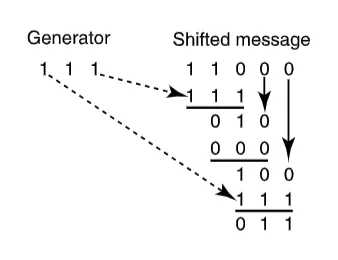
\includegraphics[width=0.75\textwidth]{../assets/ch02/ch02-2_7_1_差错检测和纠正-001.png}
    \caption{码距与检错纠错能力的几何直观。$d_{\min}=3$ 时可纠1位错误（两个纠错球不相交）；若只检错则可发现2位以内的错误。}
    \label{fig:hamming-distance}
\end{figure}

\subsection{奇偶校验：最简单的检错}

奇偶校验是在 $k$ 位数据后附加 1 位校验位，使整个 $k+1$ 位码字中"1"的个数为偶数（偶校验）或奇数（奇校验）。

以偶校验为例，发送数据 $1011001$（有4个1），校验位取0，发送 $10110010$；若发送 $1001001$（有3个1），校验位取1，发送 $10010011$。

接收方重新统计"1"的个数，若奇偶性不符，则检出错误。

\textbf{奇偶校验的局限}是显而易见的：它的最小码距为2，只能检测奇数个错误。两位同时翻转会让奇偶性恢复，错误就悄悄溜走了。因此，奇偶校验通常用于误码率很低、偶发单比特错误的场景，如内存校验（ECC 内存正是奇偶校验思想的扩展）和低速串口通信。

对于突发错误（burst error，即连续多个比特受同一个干扰影响而出错），奇偶校验几乎无能为力。需要更强大的机制。

\subsection{循环冗余校验（CRC）}

CRC 是现代数据通信中最广泛使用的差错检测方案。从以太网帧到 USB 数据包，从 ZIP 文件到卫星通信，CRC 无处不在。它强大的原因在于一个优雅的数学结构：\textbf{多项式除法}。

\subsubsection{CRC 的基本思想}

发送方和接收方事先约定一个\textbf{生成多项式} $G(x)$，其二进制表示称为生成串 $G$，长度为 $r+1$ 位（最高位和最低位均为1）。

设原始数据 $M$ 有 $k$ 位，CRC 的编码过程如下：

\begin{enumerate}
    \item 在 $M$ 后面附加 $r$ 个0，构成 $M' = M \cdot 2^r$（等价于将 $M$ 左移 $r$ 位）
    \item 用 $G$ 对 $M'$ 做\textbf{模2除法}，得余数 $R$（$r$ 位）
    \item 将 $R$ 替换掉 $M'$ 末尾的那 $r$ 个0，得到发送帧 $T = M' \oplus R = M' - R$（模2运算中加减等价）
\end{enumerate}

关键性质：$T$ 能被 $G$ 整除（模2意义下），即 $T \mod G = 0$。

接收方收到数据帧 $T'$（可能含错误）后，用同样的 $G$ 做模2除法。若余数为0，认为传输无误；若余数非零，确认发生了差错。

\subsubsection{为什么要用模2除法？}

模2运算（不进位的二进制加减法，等价于异或）是 CRC 的核心。它使得整个运算可以用线性反馈移位寄存器（LFSR）在硬件中极其高效地实现——每个时钟周期处理一位，成本几乎为零。

\subsubsection{CRC 的计算示例}

设 $M = 110$，生成串 $G = 111$（对应多项式 $x^2 + x + 1$，$r = 2$）。

\begin{enumerate}
    \item $M' = 11000$（$M$ 后追加2个0）
    \item 用模2除法计算 $11000 \div 111$：
\end{enumerate}

\[
\begin{array}{r}
    \phantom{0}110 \\
    111 \overline{)11000} \\
    \underline{111\phantom{00}} \\
    \phantom{1}100 \\
    \phantom{1}\underline{111} \\
    \phantom{11}11
\end{array}
\]

余数 $R = 11$，因此发送帧 $T = 11011$。

接收方收到 $11011$，做 $11011 \div 111$，余数为0，校验通过。若某位翻转，例如收到 $10011$，余数将不为0，立即检出差错。

\subsubsection{CRC 能检测哪些错误？}

选择合适的生成多项式 $G(x)$ 是 CRC 强大的关键。数学分析表明，一个精心设计的 $r$ 位 CRC 可以：

\begin{itemize}
    \item 检测所有单比特错误
    \item 检测所有两比特错误（只要 $G(x)$ 有至少3个因子）
    \item 检测所有奇数个错误（只要 $G(x)$ 含因子 $x+1$）
    \item 检测所有长度 $\leq r$ 的突发错误
    \item 以 $1 - 2^{-r}$ 的概率检测长度 $> r$ 的突发错误
\end{itemize}

这解释了为什么 CRC-32 在以太网中被采用：它对长度不超过32位的突发错误有100\%的检测率，对更长的突发错误仅有 $2^{-32} \approx 2.3 \times 10^{-10}$ 的漏检概率。

\subsubsection{常用 CRC 标准}

\begin{table}[htbp]
\centering
\caption{常用 CRC 标准及应用}
\begin{tabular}{llll}
\hline
\textbf{标准} & \textbf{多项式（Hex）} & \textbf{校验位} & \textbf{典型应用} \\
\hline
CRC-8       & \texttt{0x07}           & 8位  & I$^2$C 总线、传感器 \\
CRC-16-CCITT & \texttt{0x1021}        & 16位 & Modbus、USB、蓝牙 \\
CRC-32      & \texttt{0x04C11DB7}     & 32位 & 以太网、ZIP/PNG 文件 \\
CRC-64-ECMA & \texttt{0x42F0E1EBA9EA3693} & 64位 & 分布式存储、SCSI \\
\hline
\end{tabular}
\label{tab:crc-standards}
\end{table}

\subsubsection{CRC 与 TCP 校验和的分工}

实际网络中，一个 TCP 数据包同时携带两层差错保护：数据链路层的 CRC 和传输层的 TCP 校验和。这看似冗余，实则各司其职。

数据链路 CRC 在每一跳重新计算（因为链路帧头部每跳都变化），由网卡芯片硬件完成，擅长检测突发错误。但它无法捕捉路由器内部处理时引入的错误——一旦帧头重写，CRC 就被刷新了。

TCP 校验和覆盖端到端的完整路径，在软件中计算，用反码求和而非多项式除法（实现更简单），但检错能力弱于 CRC。两者互补，共同守护数据完整性——这是网络分层设计的一个典型案例：不同层次的机制解决不同范围的问题，不存在真正的"浪费"。

\subsubsection{CRC 的硬件实现}

CRC 运算的硬件实现极为优雅：用一个\textbf{线性反馈移位寄存器（LFSR）}，每个时钟周期移入一位数据，异或门放置的位置由生成多项式的系数决定。

\begin{figure}[htbp]
    \centering
    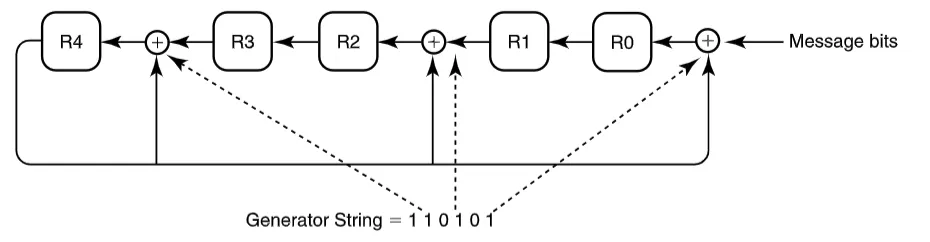
\includegraphics[width=0.85\textwidth]{../assets/ch02/ch02-2_7_1_差错检测和纠正-003.png}
    \caption{CRC 的 LFSR 硬件实现。寄存器 $R_4$ 的输出反馈到各个异或门，生成多项式系数为1的位置对应异或门。每个时钟周期移入一位，操作完成后寄存器中的内容即为 CRC 余数。}
    \label{fig:crc-lfsr}
\end{figure}

对于现代高速网络（100 Gbps 以上），逐位处理已不够快。实际实现会并行处理多位——利用查找表预计算中间结果，或用异或门矩阵一次完成 $W$ 位的 CRC 更新。

\subsection{汉明码：向纠错迈进}

检测到错误后，有两种选择：请求重传（ARQ），或在本地纠正（FEC，前向纠错）。重传简单但需要往返时延；纠错开销更大但可以零延迟恢复。卫星通信、存储系统、光纤传输等场景倾向于使用前向纠错，因为重传代价高昂甚至不可行。

\textbf{汉明码}是最经典的纠错码，由 Richard Hamming 在 1950 年发明，能纠正单比特错误、检测双比特错误。

\subsubsection{汉明码的构造}

汉明码的核心思想是：用若干\textbf{校验位}覆盖不同的数据位子集，使得每个数据位都被多个校验位"看护"。当某位出错时，出错的校验位组合能精确指出是哪一位，就像几道"探照灯"交叉定位一样。

设数据位数为 $k$，校验位数为 $r$，需满足：
\begin{equation}
    2^r \geq k + r + 1
    \label{eq:hamming-condition}
\end{equation}

校验位放在位置 $1, 2, 4, 8, \ldots$（2的幂次）处，数据位填充其余位置。校验位 $p_i$ 覆盖所有编号二进制表示中第 $i$ 位为1的位置。

以7位汉明码 (7,4)（4个数据位，3个校验位）为例。设数据位为 $d_3 d_2 d_1 d_0$：

\begin{itemize}
    \item $p_1$（位1）覆盖位 1, 3, 5, 7（二进制最低位为1）：$p_1 = d_2 \oplus d_0 \oplus d_1$
    \item $p_2$（位2）覆盖位 2, 3, 6, 7（二进制第二位为1）：$p_2 = d_3 \oplus d_0 \oplus d_2$
    \item $p_4$（位4）覆盖位 4, 5, 6, 7（二进制第三位为1）：$p_4 = d_3 \oplus d_1 \oplus d_2$
\end{itemize}

接收方重新计算这三个校验位，若某位出错，三个校验位的"符合/不符合"状态构成3位二进制数，其值恰好等于出错位的编号——0表示无错，1到7指向对应位置。将该位取反即可纠正。

这就是汉明码的精妙之处：$r$ 个校验位构成 $r$ 位二进制数，能直接"读出"错误在哪里。

\subsubsection{汉明码的局限与扩展}

基本汉明码只能纠正单比特错误。对于要求更高的场景，有以下扩展：

\textbf{扩展汉明码（SECDED）}：再添加一个整体奇偶校验位，使码距从3提升到4。可以\textbf{纠正1位错误，同时检测2位错误}（Single Error Correction, Double Error Detection）。这是 ECC 内存采用的方案——服务器内存每72位（64位数据 + 8位校验）构成一个 ECC 码字，在内存读取时实时纠正单比特翻转，是云数据中心和高可靠系统的标配。

\textbf{BCH 码（Bose-Chaudhuri-Hocquenghem）}和\textbf{Reed-Solomon 码}是更强大的纠错码族，能纠正多个错误，广泛用于 NAND 闪存、深空通信和数字广播。闪存随着使用老化会产生越来越多的比特错误，企业级 SSD 通常采用 BCH 或 LDPC 码，能纠正每1024字节中数十个错误。

\subsection{工业实践：从理论到芯片}

差错控制技术在工业界经历了从软件到硬件的彻底迁移。

\textbf{以太网}：CRC-32 由网卡硬件计算，100 Gbps 的线速下每秒处理约 150 万个帧，每帧计算耗时不足百纳秒。现代以太网芯片（如 Broadcom Tomahawk 系列）将 CRC 引擎深度流水线化，与数据接收并行完成，不引入任何额外延迟。

\textbf{数据中心互联（DCI）}：400G 及更高速率的光互联引入了\textbf{前向纠错（FEC）}作为物理层标准——KR4-FEC（基于 Reed-Solomon）在 400GBASE-R 中强制开启，以换取更大的链路功率预算，允许使用更长的光缆或更差的光模块。这是一个典型的用算力换链路裕量的工程权衡。

\textbf{AI 训练集群的 RDMA 网络}：阿里巴巴、腾讯等公司在大规模 RDMA 网络中发现，传统以太网的链路层差错控制机制（PFC 暂停帧）在遇到拥塞时会造成大范围的流量阻塞（Head-of-Line Blocking）。为此，他们开发了精细化的差错与拥塞协同控制方案——在硬件层实现 CRC 快速丢包检测，同时在 RDMA 层做选择性重传，避免整个网络因一条流的错误而停顿。这是 AI 基础设施迫使数据通信理论向工程实践演进的生动案例。

\begin{figure}[htbp]
    \centering
    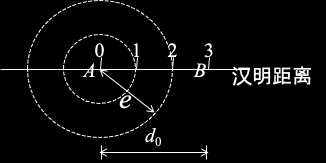
\includegraphics[width=0.85\textwidth]{../assets/ch02/ch02-2_7_1_差错检测和纠正-006.png}
    \caption{差错控制在协议栈各层的部署：物理层 FEC 对抗信道损伤，数据链路层 CRC 检测帧错误，传输层校验和提供端到端保护。各层机制互补，覆盖不同的错误场景。}
    \label{fig:error-control-layers}
\end{figure}


\section{数据链路控制}
% 来源: 19c9fb8c-0672-8939-8000-0000503faebe_2.7.2_数据链路控制.pdf
% 提取时间: 2026-02-28T22:51:18+08:00

2.7.2 数据链路控制
 在数据通信领域，随着网络规模的不断扩大和数据传输速率的日益提升，数据在传输过程中面临
诸多挑战，流量控制和差错控制应运而生。一方面，由于发送方与接收方的处理能力、传输速率等
存在差异，若发送方无节制地高速发送数据，接收方可能因来不及处理而导致缓冲区溢出、数据丢
失，进而引发网络拥塞，因此需要流量控制机制来协调双方的数据传输速率，确保数据有序流动
；另一方面，物理信道存在噪声、干扰，网络设备故障、信号衰减等因素，使得数据在传输过程中
不可避免地会出现比特错误、帧丢失等问题，为了保证接收方获取到与发送方一致的准确数据，差
错控制机制至关重要，它能有效检测错误并进行纠正或重传，保障数据的完整性和可靠性。




流量控制
定义与作用
●   流量控制主要是通过限制发送方的数据发送速率，使接收方能够及时处理接收到的数据，防止
    接收方因数据接收过快而导致缓冲区溢出，进而避免数据丢失，保证数据传输的可靠性。
实现方式主要包括
● 停等协议：这是一种简单的流量控制方式。发送方发送一个数据帧后，就停止发送，等待接收
  方的确认。接收方收到数据帧后，向发送方发送确认帧。发送方只有在收到确认帧后，才会发
  送下一个数据帧。这种方式简单，但效率较低，因为发送方在等待确认时处于空闲状态，信道
  利用率不高。
● 滑动窗口协议：该协议允许发送方在未收到接收方确认的情况下，连续发送多个数据帧。发送


                                            1
     方和接收方都有一个窗口，窗口大小表示可以发送或接收的数据帧数量。发送方可以在窗口内
     发送数据帧，接收方根据自己的处理能力和缓冲区状态，调整窗口大小并反馈给发送方。发送
     方根据接收方反馈的窗口大小来控制发送速率。例如，接收方处理数据的速度较慢，就会缩小
     窗口大小，告知发送方减少发送数据的数量。滑动窗口协议提高了信道利用率，是一种较为常
     用的流量控制方式。
停止等待协议
停止等待协议很简单，在教科书中的主要意义在于建模，帮助理解协议。为此，我们先定义一些概
念和性能指标。
 ● 传输时延 Transmission time： time taken to emit all bits into medium
 ● 传播时延 Propagation time： time for a bit to traverse the link
 ● 处理时延 Processing time (delay)： time spent at the recipient or intermediate node for
   processing
 ● 排队时延 Queuing time (delay) ：waiting time at the queue to be sent out

其中传输时延和传播时延如下图所示，中文有点类似的化可以看英文，差距就远了。




停等协议链路利用率只在传输时间大于传播时间或者帧长大于链路的比特长度的情况下较高。我们来分
析一下发送一个数据块的时间

                                                                                        2
由于ack帧的传输时延较小，进一步忽略处理时延，可以简化上面的算式



链路的利用率可以表示为




定义




B=  以比特为单位的链路长度，即比特流完全占满整个链路时，链路上的比特数;
R = 链路的数据率(bps);

                                         3
d=  链路的长度，或者说距离(m);
V = 传播速率(m/s); 空气和太空中 V 是光速；对于有线，如光纤和铜 V 约为光速的0.67倍。
L = 一个帧中的比特数(以比特为单位的帧长度)
传播时间等于距离 d 除以传播速度 V ；传输时间等于用比特表示的帧长度 L 除以数据率 R 。因
此， a 实际上代表了用比特表示的媒体长度 Rd/V 与帧长度的比值。

停等协议中有一个关键细节。如果发送方发出一帧，而接收方的确认丢失或延迟了，那么发送方会重新
发送同一帧。此时，接收方可能误认为这是新的帧，从而导致重复帧的问题。为解决这一问题，停等协
议使用一个1位序列号（0或1），这样每次发送时序列号都会变化。例如，当发送方重发序列号为0的帧
时，接收方可以识别出这是之前已接收过的帧，并忽略它，同时仍然会发送确认信号以防之前的确认丢
失。




停止等待算法的主要缺点是发送方一次只能发送一个未完成的帧，这导致链路利用率低。例如，在1.5
Mbps、往返时间45 ms的链路上，延迟带宽乘积约为8 KB。由于每个往返时间（RTT）仅能发送一个1
KB的帧，因此最大发送速率仅为182 kbps，大约是链路容量的八分之一。
滑动窗口协议


                                                       4
滑动窗口协议是一种在数据链路层实现高效数据传输的技术，它允许发送方一次性连续发送多个数据帧
到接收端，而不需要等待每一个帧的确认消息（ACK）。这种机制能够显著提高数据传输效率。在该协
议中，接收端有一个固定的缓存空间大小W，用于暂时存储接收到的数据帧；相应地，发送端也维护着
一个与之相匹配的窗口大小W，在没有收到对方发来的确认信息之前，发送方最多可以连续发送W个帧。
为了确保正确无误地传输数据并避免混淆不同批次的数据帧，每个发送出去的数据帧都会被赋予一个唯
一的序号进行标识。这个序号是通过k位二进制数来表示的，因此其取值范围为0至2k-1。当达到最大值
2k-1后，序号会重新从0开始循环使用，即采用模2^k的方式进行编号。这样做不仅能够有效利用有限的
序号资源，还能保证即使是在长时间连续通信的情况下也能保持良好的同步性。
每当接收方向发送方返回一个ACK时，除了表明已经成功接收到某些特定编号的数据帧外，还会明确指
出下一个期望接收到的数据帧编号是多少。这里的RR（Recive Ready）是接收端ACK的一种形式，RRi
即表示序号为i-1的帧都收到了，可以发送第i个帧及后续帧。




         窗口大小为7(2k-1，k=3）的滑动窗口协议，请读者自己读图理解过程

接收端可以通过发送“Receive Not Ready”报文来中断对方的数据帧流。之后，为了重新激活滑动窗口
机制，接收端必须发送一个标准的确认帧。在双向通信链路中，可以采用捎带确认（piggybacking）的
方式，即在一个数据帧中同时携带待发送的数据和对之前接收数据的确认信息。如果当前没有数据需要
发送，则发送独立的确认帧。
滑动窗口协议的性能分析也相对容易。如下图所示

                                                         5
当窗口大小 W ≥ 2a + 1 时，发送端利用率 U = 1




当窗口大小 W ≤ 2a + 1 时，发送端利用率 U = 2aW+ 1   ​




差错控制
                                           6
   在数据传输过程中，为了检测错误，通常会使用循环冗余校验（CRC）等技术。这类错误检测机制能
够识别出帧在传输过程中是否发生了改变或损坏。尽管某些类型的错误检测码足够强大，甚至能够纠正
一些简单的错误，但在实际应用中，这样的纠错能力往往伴随着较高的开销，这使得它们不太适合处理
那些可能出现在网络链路上的广泛位错误或是突发性错误。特别是对于无线通信而言，由于其环境因素
更加复杂多变，即使采用了纠错编码也可能无法完全解决所有问题。因此，在面对严重损坏的数据帧
时，最直接有效的方法就是简单地将其丢弃。
   为了确保信息能够准确无误地到达目的地，需要有一种机制来可靠地从这些被丢弃（即丢失）的帧中
恢复过来。这种可靠性功能可以在链接层实现，但很多现代通信技术却忽略了这一点。实际上，可靠的
交付服务更多是在更上层——如传输层乃至应用层提供。关于究竟应该在哪一层级实现这一功能，目前
仍存在争议，这取决于多种因素，包括但不限于系统设计需求、性能考量以及成本效益分析等。我们在
此讨论可靠交付的基础概念，因为这些原则不仅适用于链接层，而且贯穿整个协议栈的不同层级，但请
注意，我们的讨论并不局限于链接层的功能。
   实现可靠交付主要依赖于两种基本机制：确认和超时。确认过程涉及发送一个小控制帧（通常称为
ACK，即Acknowledgment的缩写）回给发送方，以表明先前发送的数据帧已被成功接收。这里的“控制
帧”指的是不包含任何实际用户数据的消息头部；然而，有些协议允许将ACK信息附加到反方向流动的数
据帧之上。一旦原始发送者收到这个确认消息，就表示其之前发出的信息已经安全抵达目的地。如果发
送方在合理时间内没有接收到预期的ACK响应，则会触发一个称为“超时”的事件，并导致该帧被重新发
送。通过这种方式，可以有效地保证数据的完整性与一致性。
   利用确认和超时机制来实现可靠交付的技术通常被称为自动重传请求（ARQ, Automatic Repeat
reQuest）。接下来的部分将介绍三种不同的ARQ算法，我们将采用一种通用的语言来进行描述，而不是
深入探讨特定协议的具体实现细节。

ARQ包含三种机制
 ● Stop-and-Wait Automatic Repeat Request
 ● Go-Back-N        Automatic Repeat Request
 ● Selective Repeat Automatic Repeat Request


停等ARQ
主要针对以下两种类型的差错
 ● 帧丢失 （lost frames）
    ○ 帧没有达到另一方
 ● 帧损伤 （damaged frame）
    ○ 帧到达，但是一些比特有差错



                                                      7
源点发送一个数据帧，等待ACK
 ● 保持一个发送帧的拷贝
 ● 在终点确认返回前，源点不发送其他帧

1）帧损伤
 ● 接收端检测到差错，丢弃该帧？
 ● 发送端超时重传

2）ACK损伤
 ● 发送端超时重传
 ● 接收端收到用两份相同编号的帧
 ● 使用 ACK0 / ACK1 来确认希望接收的帧
    ○ ACKi means“I am ready to receive frame i”

执行过程如下图所示




Go-Back-N ARQ
基于滑动窗口流控机制,没有收到确认的帧的最大数目取决于窗口大小
如果没有差错，使用ACK确认接收就绪
                                                  8
 ● ACKi 表示 “I am ready to receive frame i” 或者 “I received all frames between i and my
   previous ACKs
如果错误发生，为错误帧发送rejection (negative ACK)
 ● 接收端丢弃该帧和所有后来收到的帧，直到错误帧被正确接收
 ● 发送端必须重传有差错的帧和差错帧后所有已经传输过的帧



a) 帧损伤 （Damaged frame）
 1. 接收方检测到第 i 帧中的错误
 2. 接收方发送“拒绝 i”

 3. 发送方收到“拒绝 i”

 4. 发送方重新传输第 i 帧及其后续所有帧



（1）接收端乱序
 1. 发送方发送帧 i
 2. 发送方发送帧 i+1
 3. 接收方收到失序的帧 i+1
 4. 接收方发送“拒绝 i”
 5. 发送方返回到帧 i，并重新传输它以及所有后续帧



（2）计时器超时
 1. 第i帧丢失，且没有发送额外的帧
 2. 接收方什么都没收到，既不返回确认也不返回拒绝

 3. 发送方超时，并发送一个P比特设置为1的确认帧（这实际上是一个ACK请求命令）

 4. 接收方将此解释为一个ACK请求命令，并用其期望的下一帧的编号（i）进行确认

 5. 发送方随后重新传输第i帧




                                                                                    9
Selective-Reject ARQ
选择性重传ARQ（Automatic Repeat reQuest）是一种仅针对被拒绝帧或超时帧进行重传的机制。在此
机制中，接收端会对接收到的后续帧进行缓存，从而最小化需要重传的帧数量。然而，这一方法要求接
收端具备足够大的缓存空间以支持帧的暂存。与此同时，发送端与接收端的逻辑设计更为复杂，主要体
现在以下方面：
 ● 接收端需具备按照正确顺序重组帧的能力；
 ● 发送端需能够识别并仅重传出错或失序的帧。
   这种机制特别适用于传播时延较长的卫星链路场景，在此类环境中，其高效的重传策略能够显著提
   升通信性能并降低资源浪费。




                                                         10
选择拒绝ARO对窗口大小的限制比返回N ARO更加严格。考虑这样一种情况，选择拒绝ARO序号字段的
长度为3比特，窗口大小可达到7个帧，那么设想以下情况:
1.站点A向站点B发送从帧0到帧6的所有帧。
2.站点B接收到所有的7个帧，并以RR 7作为累积确认。
3.由于噪声脉冲序列，RR 7丢失。
4.计时器超时，A重传帧0。
5.B已经将它的接收窗口向前滑动至可接受帧7,0,1,2,3,4 和5。因此它会认为丢失的是帧7，而它接收到的
是一个新的帧0，可以接受。
上述情况的问题在于发送窗口和接收窗口之间出现了重叠部分。要克服这个问题，最大窗口值必须小于
序号范围的一半。对于上述情况，只允许4个未被确认的帧存在，就不会发生混淆。一般情况，对于k比
特的序号字段，它提供的序号范围为2，而最大窗口值则限制在 2k−1 内。
性能分析
停等ARQ


                                                      11
对与停等ARQ，我们已经知道在无差错的情况下，停等协议的链路利用率是 1 +1 2a 。                     ​




如果有差错出现，则为利用率除以 Nr , Nr 是一个帧的传输次数的期望值
                                 ​       ​




         传输次数) = ∑(i × P [i次传输]) = ∑(iP (1 − P )) = 1 −1 P
                       ∞                         ∞
Nr = E(
   ​                         ​                         ​
                                                           i−1
                                                                     ​




                       i=1                       i=1

因此停等ARQ的 链路利用率是 U = 11 +− 2a
                          P
                                             ​




          ∞
用到公式 ∑(iX i−1 ) = (1 −1X)2
               ​                     ​       −1≤X ≤1
         i=1


Selective-Reject ARQ




Go-back N ARQ
                                                                         12
Each error generates a requirement to retransmit K frames rather than just
one frame.


where f(i) is the total number of frames transmitted if the original frame must be
transmitted i times




                                                                                     13
设备内流量控制
在芯片间链路上，链路错误非常罕见，恢复操作可以交给原始源计算机处理。因此，可以应用没有与错
误控制交织在一起的流量控制方法。
这张图展示了一种简单的方法，用来管理路由器内部芯片之间数据传输的流量控制。发送方有一个叫“信
用寄存器”（CR）的东西，刚开始时，它的数值等于接收方提供的缓冲区数量。发送方只有在CR的值大
于0的时候才会发送数据，并且每发送一个数据，CR的值就会减1。在接收方那边，每当它从缓冲区里处
理完一个数据，就会告诉发送方“我又有空位了”，这就是所谓的“信用”。当发送方收到这个“信用”消息
后，就会把CR的值加1，表示可以继续发送数据了。




       图片加载失败
                   基于credit的流量控制
提高性能
如果路由器分配的缓冲区数量够大—具体来说，比线路速度和往返延迟的乘积（也叫“管道大小”）还
多，那么数据就可以以全速传输。但在实际的路由器中，问题来了：通常有好几类不同的流量在共享同
一条链路。一种简单的解决办法是，把缓冲区分成几块，每类流量各自独占一部分。但这会浪费资源，
因为每类流量都需要预留出“管道大小”的缓冲区（比如10个信元缓冲区）。如果有大量类别，所需缓冲
区的数量会迅速膨胀，可能会超出路由器芯片上的静态随机存取存储器（SRAM）容量。要知道，FPGA
（现场可编程门阵列）上的SRAM本来就特别有限。

                                               14
而且，给每个类别都分配完整的管道大小其实很浪费，毕竟所有类别同时发送数据的情况很少见，即使
发生了，每个类别也只能分到链路带宽的一小部分。所以，共享缓冲区是个更合理的选择。最简单的办
法是把缓冲区分成两部分：一部分是大家共用的公共池，另一部分是每类流量专属的私有池。
一个简单的设计是，把数据信元和信用标记为属于公共池或私有池，这样可以避免不同类别互相干扰。
不过，这个方法还需要一些额外的机制，确保某个类别不会占用超过管道大小的缓冲区。
一种更优雅的方案，可以让缓冲区共享而不用标记信元。大致思路是这样的：接收方的缓冲区被分成两
部分，一部分是每类流量的私有池，包含固定数量的缓冲区（称为Min）；另一部分是一个公共池，大小
为总缓冲区减去所有私有池的总和（即B - N * Min，N是类别数量，B是总缓冲区大小）。管道大小用
Max表示。
这个协议有两种运行模式：拥塞模式和非拥塞模式。
 ● 在非拥塞模式下，每个类别最多可以占用Max个缓冲区，自由地发送数据。
 ● 在拥塞模式下，每个类别只能占用Min个缓冲区，发送受限。
    下游节点的所有缓冲区都是通用的，任何缓冲区都可以分配给任何类别的传入数据。通过精心设计
    两种模式之间的切换规则，既防止了死锁，也避免了数据丢失，同时实现了缓冲区的高效共享。
为了在不标记信元的情况下实现对私有池的管理，发送方需要跟踪两个数字：
 1. 总的未处理信元数 S ，也就是已发送的信元数减去收到的确认数。
 2. 每个类别i的未处理信元数 Si 。
    当总的未处理信元数 S 小于N * Min（即私有池还没用完时），协议处于非拥塞模式，只要某个类
                 ​




    别的未处理信元数 Si 不超过Max，它就可以继续发送数据。
    但当 S 达到或超过N * Min时，链路被认为进入了拥塞状态，此时每个类别会被限制使用私有池，
             ​




    确保 Si 不超过Min。
    简单来说，这种缓冲区共享协议的工作原理是这样的：
        ​




 ● 在轻负载时，只有少数类别在活动，这些活跃类别可以占用更多的缓冲区（最多Max个），尽可能
    快速传输数据。
 ● 在重负载时，所有类别都在活动，每个类别至少还能保证有Min个缓冲区可用，从而避免饿死。

可以添加滞后机制来防止两种模式之间的振荡。也可以将基于信用的流量控制的缓冲区共享思想扩展到
基于速率的流量控制的速率共享，例如使用漏桶算法。
提高可靠性
上一小节中概述的协议非常有效地利用了有限的接收方SRAM缓冲区，但对故障的鲁棒性不足。在了解如
何使更复杂的流量控制协议对故障具有鲁棒性之前，先从上图中描绘的更简单的信用协议入手会更明
智。
直观地说，图中的协议就像是在两家银行之间转账：“银行” 是发送方和接收方，信用和信元都算作
“钱”。很容易看出，在没有错误的情况下，系统中的总 “钱数” 是守恒的。更正式地说，设CR为信用寄
                                                  15
存器，M为从发送方到接收方传输中的信元数，c为反向传输中的信用数，Q为接收方占用的信元缓冲区
数。
那么，很容易看出（假设初始化正确，并且链路上没有信元或信用丢失），该协议在任何时刻都保持以
下属性：(CR + M + Q + C = B)，其中B是接收方的总缓冲区空间。这种关系被称为不变量，因为只要
协议正常工作，它就始终成立。建立这个不变量是协议初始化的工作，而容错机制的工作是维护这个不
变量。如果始终维护这个不变量，那么系统就永远不会丢弃信元，因为传输中的信元数加上存储的信元
数永远不会超过分配的缓冲区数量。
简单的逐跳流量控制方案存在两个潜在问题。第一，如果初始化不正确，那么发送方可能会有过多的信
用，这可能导致信元被丢弃。第二，由于链路错误，某个类别的信用或信元可能会丢失。即使是芯片间
链路也难免会偶尔出现位错误；在高链路速度下，这种错误每小时可能会发生几次。第二个问题可能会
导致速度减慢或死锁。
许多实现者可能会错误地认为这些问题可以通过简单的机制来解决。一种直接的反应是认为这些情况不
会发生或很少发生。其次，有人可能会尝试使用定时器来检测可能的死锁，以解决第二个问题。不幸的
是，很难区分死锁和接收方非常缓慢地取出信元的情况。更糟糕的是，整个链路可能会慢得像爬行一
样，导致路由器性能下降；而且结果很难调试。




                  图2标记算法的三个步骤
这些问题可能可以通过路由器重置来解决，但这是一种严厉的解决方案。相反，可以考虑以下重新同步
方案。为了清晰起见，该方案通过图2中一系列的改进来呈现。

                                                      16
在最简单的同步方案（方案1，图2）中，假设协议定期发送一个特殊标记的信元，称为标记信元。在标
记信元返回之前，发送方停止发送数据信元。在接收方，标记信元在被发送回上游节点之前先流经缓冲
区。很容易看出，在标记信元返回后，它已经 “清空” 了管道中的所有信元和信用。因此，在标记信元返
回的那一刻，协议可以将CR设置为最大值（B）。方案1很简单，但需要发送方定期空闲以进行重新同
步。
因此，方案2（图2）对方案1进行了改进，允许发送方在发送标记信元后发送信元；然而，发送方会在一
个寄存器（例如，CSM，用于记录 “自标记信元发送以来发送的信元数”）中跟踪自标记信元发送以来发
送的信元。当标记信元返回时，发送方会考虑自标记信元发送以来发送的信元，调整修正值，从而将CR
设置为(B - CSM)。
方案2的主要缺陷是无法限制标记信元在接收方队列中停留的延迟。这会导致两个问题。第一，很难确定
该方案需要多长时间才能自我纠正。第二，为了使标记信元方案本身可靠，发送方必须定期重新传输标
记信元。如果无法限制标记信元的往返延迟，发送方可能会过早重新传输，这使得在不增加序列号复杂
性的情况下，很难将标记信元的响应与请求匹配起来。
为了限制标记信元的往返延迟，方案3（图2）让标记信元绕过接收方队列并立即 “反射回来”。然而，这
要求标记信元返回时携带接收方在接收到标记信元那一刻的空闲信元缓冲区数量F。然后，当标记信元返
回时，发送方将信用寄存器CR设置为(F-CSM)。
标记信元方案是一种称为快照的经典分布式系统技术的特殊实例。非正式地说，快照是一种分布式审
计，它生成分布式系统的一致状态。我们基于标记信元的快照与Chandy和Lamport（1985）中描述的经
典快照略有不同。然而，重要的是，快照可用于检测任何分布式算法的不正确状态，并且可以在两节点
子系统中高效实现，以使任何此类协议具有鲁棒性。特别是，同样的技术（Ozveren等人，1994）可以
用于使15.1.1节中更复杂的流量控制同样具有鲁棒性。
特别是，标记信元协议使信用更新协议具有自稳定特性，即它可以从任意错误（包括链路错误）以及损
坏寄存器的硬件错误中恢复。这是一种极端形式的容错能力，可以在不牺牲性能的情况下极大地提高子
系统的可靠性。
总之，对于两节点系统的通用技术是写下协议不变量，然后设计一个定期快照来验证不变量，并在必要
时进行纠正。
内部链路条带化
路由器内部的流量控制是由互连长度不断增加和速度不断提高这两个因素驱动的。另一方面，路由器内
部的链路条带化是由互连速度较慢所驱动的。如果串行线路速度不够快，设计者可能会在内部通过多个
串行链路对信元进行条带化处理。
在大多数应用中，每个通道的延迟是可变的；在每个通道上发送数据包的最快时间和最慢时间之间存在
很大的偏差。因此，一个好的条带化算法的目标是在存在任意偏差的情况下实现先进先出（FIFO）交

                                                   17
付，路由器不应因内部机制而重新排序数据包，并且在面对链路位错误时具有鲁棒性。
为了理解为什么实现这些目标的组合可能会很困难，可以考虑循环轮询条带化。发送方以循环轮询的顺
序在通道上发送数据包。然而，如果不修改数据包，循环轮询并不能提供FIFO交付。通道可能存在不同
的延迟偏差，因此数据包在接收方的物理到达顺序可能与其逻辑顺序不同。如果没有序列号信息，数据
包可能会持续乱序。
可以通过添加数据包序列号来使循环轮询方案保证FIFO交付，接收方可以使用该序列号对数据包进行重
新排序。然而，许多实现方案不希望添加序列号，因为这会增加信元开销并降低路由器的有效吞吐量。
提高性能
为了在不增加序列号开销的前提下实现有序传输，主要思路是将物理接收和逻辑接收解耦。物理接收容
易受到延迟偏差导致的乱序影响，而逻辑接收则通过缓冲机制以及让接收方采用与发送方相同的算法来
取出信元，从而消除乱序问题。
例如，假设发送方使用一个循环指针，以循环轮询的方式在发送通道上对信元进行条带化处理。这样，
信元A会被发送到通道1，之后发送方的循环指针会递增到2。下一个信元B则会被发送到通道2，以此类
推。
接收方会缓存接收到的信元，但在信元到达时不会立即出队。相反，接收方也会维护一个初始值为通道1
的循环指针。接收方会在通道1等待接收信元，当有信元到达时，该信元会出队，然后接收方会移动到通
道2等待接收信元。因此，如果延迟偏差导致信元B（在信元A被发送到通道1之后，被发送到通道2）比
信元A先到达，接收方不会在信元A之前将信元B出队。相反，接收方会等待信元A到达，在将信元A出队
后，才会移动到通道2，并在通道2将等待的信元B出队。
提高可靠性
发送方和接收方之间的同步可能会因为单个信元的丢失而被破坏。在前面提到的循环轮询示例中，如果
在通过三条链路发送的大量信元中，信元A丢失了，接收方将会按D、B、C、G、E、F……的顺序交付数
据包，从而永久性地打乱信元顺序。




                                               18
图3 错序与恢复：接收端的最终输出为D、B、C、E、F、G、H、I，并且在逻辑上接收到E之后实现了同
步。
对于交换结构和某些链路，人们可能会认为信元丢失的情况非常罕见（比如一年一次）。然而，这样的
假设应该会让设计者感到不安，尤其是当一次丢失就可能从那时起造成永久性损害的时候。为了防止单
个信元丢失后造成永久性损害，发送方必须定期与接收方重新同步。
将一轮定义为在返回起始通道之前，对连续通道的一系列访问。在每一轮中，发送方会通过所有通道发
送数据。同样，在每一轮中，接收方会从所有通道接收数据。为了实现重新同步，发送方会维护所有通
道的轮次编号（初始值为R0），接收方也会这样做。
因此，在图3中，发送完A、B和C后，发送方所有通道的编号都变为R1。然而，在接收方，只有通道1的
编号为R1，其他通道仍为R0，这是因为在接收方的第一轮循环扫描中，第二和第三个通道还未被访问
到。当发送方或接收方的循环指针递增到某个通道时，相应的轮次编号也会递增。
实际上，轮次编号可以被视为每个通道隐含的序列号。因此，信元A可以被认为具有序列号R1，下一个在
通道1发送的信元D则可以被认为具有序列号R2，以此类推。
因此，在图3的场景2中，发送方继续在通道1发送信元D，在通道2发送信元E。接收方仍在通道1等待信
元，最终收到了信元。此时，场景切换到场景3，接收方按顺序输出信元D和B，然后移动到通道3，最终
在通道3收到信元C。
基本上，场景2中的乱序问题是由于接收方在接收方的R1轮中，将在R2轮发送的信元（即D）出队导致
的。这就提出了一种简单的同步通道轮次编号的策略：发送方应该定期在每个通道上向接收方发送其当

                                                19
前的轮次编号。为了减少开销，这样的标记信元应该在发送数百个数据信元之后再发送，代价是在信元
丢失后可能会有数百个信元出现乱序。
为简洁起见，图3中的示例假设在通道1发送信元D之后发送标记信元，其他通道上标记信元的发送情况未
展示。因此在场景3中，可以看到发送方在通道1发送了包含当前轮次编号R2的标记信元。
在场景4中，接收方按顺序输出了信元D、B和C，现在又在等待通道1上的信元。此时，包含R2的标记信
元到达。
只有当标记信元位于缓冲区头部，且循环指针指向相应通道时，接收方才会处理该标记信元。处理遵循
以下四条规则：（1）如果标记信元中的轮次编号严格大于接收方当前的轮次编号，说明标记信元到达过
早，此时循环指针递增；（2）如果轮次编号相等，那么后续的信元轮次编号会更高，因此循环指针递
增，同时标记信元被移除（但不会输出）；（3）如果标记信元中的轮次编号比当前通道的轮次编号小
1，这属于正常无错误的情况，后续的信元轮次编号将是正确的，此时标记信元被移除，但接收方的循环
指针不递增；最后，（4）如果标记信元中的轮次编号比当前通道的轮次编号小k（k>1），则表明发生了
严重错误（除信元丢失外），发送方和接收方应该重新初始化。
因此，在场景4中，规则2适用：标记信元被销毁，循环指针递增。此时，可以很容易看出，发送方和接
收方现在已完全同步，因为对于接收方的每个通道，到达该通道时的轮次编号与下一个信元的轮次编号
相等。因此，该过程在场景4中正确地将信元E出队，在场景5中将信元F出队，最后在场景6中将信元G出
队，顺序得以恢复。
因此，增强后的负载均衡算法能够快速从错误中恢复（从发送标记信元到接收标记信元的时间加上单向
传播延迟）。图3所示方法的基本技术是通过定期单向发送标记信元，检测每个通道上的状态不一致。

对于负载均衡，除了每个通道上用于关联发送方和接收方轮次编号的单向不变量之外，还有一个全局不
变量，该不变量确保在假设没有数据包丢失的情况下，通道轮次编号之间的差异不会超过1。在因数据包
丢失导致违反该不变量后，接收方会通过跳过某些信元来强制执行该节点不变量。
即使在可以给信元添加序列号的情况下，逻辑接收也有助于简化重新排序的实现过程。一些重新排序器
使用快速并行硬件排序电路来重新组装数据包。如果采用逻辑接收，这种电路就有些多余了。逻辑接收
在正常情况下已经足够，在极少数出现错误的情况下，通过缓慢扫描查找匹配的序列号就足够了。要知
道，在芯片间链路上，错误应该是非常罕见的。需要注意的是，如果添加了序列号，就能保证FIFO交
付，这与图3中的协议不同。
分布式内存
数据包缓冲区是路由器硬件的重要组成部分，原因有三：规模、普遍性和服务质量。
第一，随着速度的提升，数据包缓冲区的规模也在不断增大。经典的经验法则是，交换机应缓存RTT×R
比特的数据以应对拥塞（其中RTT是通过路由器的TCP流的平均往返时间。假设从海岸到海岸的延迟约
                                              20
为250毫秒，一个100 Gb/s的接口需要25 Gb的内存，这在商用动态随机存取存储器（DRAM）的容量范
围内，但比高速静态随机存取存储器（SRAM）大得多。
第二，数据包缓冲区在路由器中无处不在。两个重要的例子是在输入缓冲交换机的虚拟输出队列
（VOQ）输入端（由于对输出端口的竞争），以及在输出端口（由于输出链路拥塞）。然而，在实际的
路由器中，还有许多其他使用缓冲区的地方，包括上一节提到的数据包在交换结构中进行条带化处理时
的重新排序缓冲区，以及组播复制缓冲区。
第三，正如我们之前所见，服务质量（QoS）使路由器缓冲变得复杂。服务提供商使用的路由器，如思
科GSR 12000路由器，每个线路卡大约维护2000个队列，而边缘路由器，如瞻博网络的E系列，则提供
多达64000个队列，以实现精细的QoS控制。
如今，路由器缓冲区的主要问题在于，一旦链路速度超过10 Gb/s，一个最小尺寸为40字节的数据包会
在32纳秒内到达。这意味着每隔16纳秒就需要对内存进行一次数据包的写入或读取操作（请记住，数据
包必须先写入并存储，然后读取出来才能发送出去）。如果使用一个访问时间为50纳秒的标准DRAM，
这是无法实现的。同样，使用具有这种容量的SRAM成本太高且功耗太大。
一种可能的方法是设计具有更短访问时间的新型DRAM。DRAM的访问时间取决于其架构。从理论上讲，
可以通过在内部设计更小的存储体来提高DRAM的速度，甚至可以制造出访问时间为（例如）20纳秒的
DRAM。不幸的是，随着速度的提升，这种方法并不具有扩展性。此外，额外的存储体开销需要更大的
芯片面积，导致面积与成本之间的权衡难以接受。尤其在当今世界，路由器内存只是整个DRAM市场的
一小部分，而计算机内存的严格成本压力主导着DRAM市场，这种情况更为明显。
提高性能
正如上一节中，当链路成为瓶颈时我们对数据包进行跨链路条带化处理一样，许多路由器制造商通常会
在路由器内部对数据包进行跨DRAM条带化处理。这看似简单：数据包到达时，会被写入当前未被写入
的任何一个DRAM中。当一个数据包离开时，只有在其所在的DRAM空闲时，才会从该DRAM中读取数
据。需要注意的是，DRAM协议允许对同一DRAM中不同存储体的读写操作进行一定程度的流水线处理，
即使DRAM本身尚未完全完成之前对这些不同存储体的读写请求。
不幸的是，虽然这种方法在大多数情况下或系统负载较轻时可能运行良好，但在高负载和特定的访问模
式下，效果可能会很差。一些供应商试图通过增加一些加速机制来降低这种情况发生的可能性，但这种
方法仍然是基于统计的，难以准确描述。
如果需要保证最坏情况下的性能，尤其是在有严格QoS约束的情况下，这种方法是不正确的。特别是，
有几家测试公司能够发现路由器中的此类缺陷。我们需要在使用全SRAM缓冲区这种正确但昂贵的解决方
案，和跨DRAM存储体条带化这种基于统计但不正确的解决方案之间，找到一种折中的方法。
Wang等人（2010）提出了一种流水线内存系统，在以下方面具有强大的性能。该内存系统在时间t接收
到读或写请求时，能以极高的概率（例如 1 − 10−25 ）保证在 t + Δ （其中 Δ 是一个恒定延迟）时
刻准确完成请求，且适用于包括最坏情况在内的任意内存读写模式；它能够在每个SRAM周期处理一个请
                                                     21
求，因此具有与SRAM相同的吞吐量。这种统计保证是通过最坏情况大偏差理论严格证明的。该内存系统
是通用的：它不仅可以支持路由器数据包缓冲区，还可以支持其他路由器或防火墙功能，如网络流状态
的存储、访问和维护。不过，这种内存系统也有一个缺点：固定延迟 Δ 可能超过1000个SRAM周期，
即超过几微秒，对于当今的路由器和交换机来说，这个延迟有点过高。相比之下，伊耶论文中提出的内
存系统在专门用于路由器数据包缓冲区时，能提供严格的绝对（而非统计）延迟保证。它通过利用路由
器数据包缓冲区特定的内存访问模式来实现这一点。
提高可靠性
使用静态随机存取存储器（SRAM）作为动态随机存取存储器（DRAM）存储体阵列的前端缓存。通过巧
妙的算法和 “分级SRAM”，可以证明该方案能够模拟单个大型SRAM的行为。然而，要更精确地实现这
个想法，还需要做更多工作。首先，我们必须定义头部和尾部队列的大小，并证明这些大小与队列总大
小相比是较小的。其次，也是最重要的，我们必须定义算法，以确定哪些数据包从SRAM尾部缓存读入
DRAM（在输入侧），以及哪些数据包从DRAM读出到SRAM头部缓存（在输出侧）。
为了定义各种算法（具有不同的权衡）所需的头部和尾部缓存大小，我们需要以下符号。首先，很明显
DRAM与SRAM速度之比是一个基本参数。如果DRAM的访问时间是50纳秒，SRAM的访问时间是5纳
秒，那么在一次DRAM写入操作的时间内，有 10 = 50 ÷ 5 个数据包可以到达SRAM。因此，如果内存
以64字节长度的单元工作，那么缓存块（这也是从DRAM读取和写入的块大小）至少必须是640字节。
以内存单元表示的DRAM与SRAM速度之比是第一个基本参数b。
第二个基本参数是队列数量Q。显然，队列越多，SRAM和DRAM之间的潜在积压就越大。在最坏的情况
下，在等待DRAM写入时，每个队列都可能有小数据包到达。需要注意的是，每个队列只能进行一次
DRAM写入操作；不能像在同一队列中那样跨队列批量处理数据包。在写入DRAM时，通过复杂的指针管
理，理论上可以跨队列批量处理数据包。但不幸的是，在从DRAM读取数据时，这就失去了意义。从
DRAM读取的一个块现在可能包含来自不同队列、大小不一的数据，这种“分散收集”式的读取方式无法
满足动态且不可预测的读取访问模式下每个队列不同的速度需求。
尾部缓存最容易理解。直观地说，控制器会在尾部缓存中为每个队列收集最多b字节的数据，并在可能的
情况下，以一次更大的DRAM块写入操作将数据写入DRAM。因此，尾部队列大小设为 Qb 是合理的。
另一方面，头部缓存更为复杂，因为控制器必须应对来自任何队列的对抗性读取模式，而这种模式的数
量组合非常庞大。
令人惊讶的是，如果头部缓存稍微大一些（与 QblogQ 成正比），该算法就能保证在最坏情况下，无
论请求哪个队列（当然，前提是该队列有数据），头部缓存都不会出现饥饿现象。同样直观地，人们可
能会想到类似于最早截止时间优先的算法（但要证明最坏情况下 QblogQ 的界限仍需要深入思考）。
其思路是首先从DRAM中补充头部缓存中字节数最少的队列，因为对手可能接下来就会选择这个队列。
论文将此称为“最缺额队列优先”算法。由于可能存在流水线操作，实际的缺额概念更为微妙。不过，忽
略流水线操作，可以认为缺额最大的队列就是字节数最少的队列。

                                                    22
此外，如果已知队列的行为并非完全对抗性的，那么头部缓存的大小还可以进一步减小。
本节中描述的分布式内存算法产生了巨大的影响。这些算法首先在伊耶和麦基翁创立的一家名为Nemo的
初创公司中实现商业化。Nemo被思科收购后，开始对思科路由器产生重大影响。根据伊耶论文
（Sundar，2008年）中的一些估计，仅在思科内部，分布式内存每年就被用于7条以上产品线中的数百
万个芯片，通过用廉价的片外DRAM替代SRAM，每年节省数亿美元，同时支持数千个队列。虽然更复杂
的算法很少被使用，但简单的“最缺额队列优先”算法在思科绝大多数头部缓存实现中都有应用。对于尾
部缓存，大小为 Qb 的简单动态分配缓存被普遍使用。
除了节省内存，其他优点还包括降低功耗、减少专用集成电路（ASIC）上用于处理多个存储器的引脚数
量，以及提高利用率。更高的利用率来自于将数据批量处理为大小为b的块。一个令人惊讶的附带好处
是，消除了内部SRAM单元大小为64字节时发送65字节数据包所带来的棘手问题。当将一系列65字节的
数据包批量存储在大小为 b = 640 字节（例如）的尾部缓存中时，内存碎片化问题就不那么严重了。
第二个微妙的优点是，这些经过证明的在最坏情况下也能保证性能的队列消除了数据包丢失的情况：这
在存储市场以及其他对服务质量（QoS）要求严格、需要严格限制延迟的应用中至关重要。
异步更新
与快速搜索操作并发执行的原子更新，是第11章和第10章中所有增量算法的必要组成部分。例如，假设
trie树节点X指向节点Z。通常，插入一个前缀需要添加一个新节点Y，使得X指向Y，Y再指向Z。由于数
据包以线速并发到达，更新过程必须尽量减少对搜索过程的阻塞。在不使用锁的情况下，最简单的方法
是首先完全构建节点Y并使其指向Z，然后通过一次原子写入操作，将节点X的指针转向指向Y。
然而，一般来说，这样的设计存在许多需要精细处理的地方，尤其是在面临流水线等复杂情况时。为了
说明其中潜在的陷阱以及正确推理的重要性，让我们考虑下面这个取自第一个网桥实现的例子。
在第10章研究的第一个网桥产品中，网桥使用二分查找。假设有一个包含不同键B、C、D、E的长列表，
并且在最后一个（最大的）键之后有空闲空间。现在考虑添加一个新条目A的问题。有两种标准方法来处
理这个问题。
第一种方法是模仿数据库的原子更新技术，保留二分查找表的两个副本。插入A时，搜索操作在旧副本上
进行，而A被插入到第二个副本中。然后，通过一次原子操作，更新过程翻转一个指针（芯片使用该指针
来确定要搜索的表），使其指向第二个副本。
然而，这会使所需的存储空间翻倍，尤其是当内存为SRAM时，成本很高。因此，许多设计者更喜欢第二
种选择：通过将所有大于等于B的元素向下移动一个位置，为A创建一个空位。
提高性能
为了减少内存需求，更新操作必须在与搜索操作相同的二分查找表上进行。例如，在\begin{figure}[htbp]
\centering
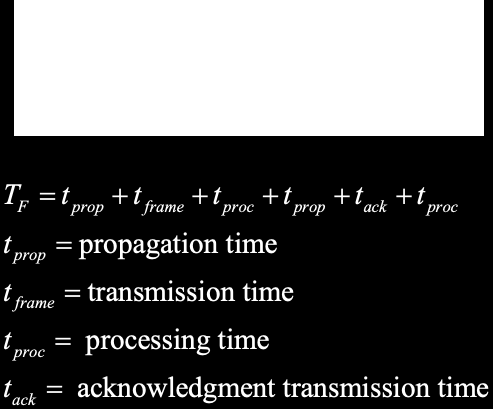
\includegraphics[width=0.8\textwidth]{../assets/ch02/ch02-2_7_2_数据链路控制-004.png}
\end{figure}
图15.4中插入元素A
时，更新操作必须将元素B、C和D向下移动一个位置。
                                                23
如果更新和搜索的设计者不同，那么对于更新设计者的常规要求通常是确保搜索过程看到的二分查找表
是一致的，且表中的键值各不相同。如果不等到完整的更新操作结束就允许进行搜索，似乎很难满足这
个要求。由于对于一个包含32000个元素的网桥数据库，一次更新可能需要很长时间，所以这种等待更
新结束再进行搜索的方式是不可接受的。
因此，可以考虑放宽要求（P3），允许二分查找表中存在重复的键值，只要该表保持有序即可。毕竟，
只要表是有序的，存在两个或更多相同值的键并不会影响二分查找的正确性。
因此，在图15.4中为A创建空位的过程是这样的：先为D创建两个条目，接着为C创建两个条目，然后为B
创建两个条目，每次操作都只对表进行一次写入。最后一步，将A写入B的第一个副本所在的位置。
为了使二分查找芯片保持简单（见第10章），路由处理器负责更新操作，而芯片负责搜索操作。表格存
储在一个单独的片外内存中；内存、处理器和芯片这三个设备可以通过一条公共总线相互通信。抽象地
说，搜索和更新这两个独立的过程同时访问内存。由于使用锁来协调内存访问会导致内存访问速度变
慢，所以这种方式并不可行。
鉴于新的规范允许存在重复键值，有人可能会试图采用最简单的内存读写原子性方式。搜索操作读取内
存，更新操作进行读写；搜索和更新的内存操作可以任意交错进行。一些实现者可能认为，因为二分查
找即使在存在重复键值的情况下也能正确工作，所以这样就足够了。
不幸的是，如图15.4所示，这种方式并不正确。在场景开始时（最左边的图），只有B、C和D分别位于
表的第一、第二和第三个条目中，第四个条目为空。对B进行搜索时从第二个条目开始；与C比较后，二
分查找算法判断应该移动到上半部分，而这里只有第一个条目。
接下来，搜索操作被延迟，同时更新操作开始通过从下往上写入重复项的方式插入A。当更新操作完成
时，B已经移动到了第二个条目。当搜索操作最后检查第一个条目时，它找到了A，并错误地得出B不在
表中的结论。
只要简单地尝试进行正确推理，就能直接发现这类反例。二分查找的标准不变量是，要么正在搜索的元
素（例如B）在当前的二分查找范围内，要么B不在表中。问题在于，更新操作可能会将正在搜索的元素
移动到当前范围之外，从而破坏这个不变量。
在网桥应用中，这种错误的唯一后果是，到达已知目的地的数据包可能会被泛洪到所有端口。这只会稍
微降低性能，不太可能被外部用户注意到！
提高可靠性
对于图15.4中的反例，一种惊慌的反应可能是放弃单副本更新，退回到更安全的双副本方式。然而，这个
反例只是表明，搜索操作必须在没有更新操作干扰的情况下完成。如果能做到这一点，二分查找的不变
量就能保持成立，结果的正确性也能得到保证。这个反例并不意味着相反的情况，即整个更新操作必须
在没有搜索操作干扰的情况下完成。相反的这种特性限制过多，会大大降低搜索速度。


                                                24
有一些简单的方法可以确保搜索操作在没有更新操作干扰的情况下完成。第一种方法是改变架构模型，
毕竟算法学就是一门通过改变问题来适应我们有限智慧的艺术。可以将所有更新写入操作集中通过搜索
芯片进行。当更新操作想要执行写入时，它向搜索芯片提交写入请求并等待确认。搜索芯片完成当前的
搜索周期后，执行所需的写入操作并发送确认信息。然后，搜索芯片可以继续处理下一个搜索任务。
第二种方法与网桥的实现方式更相符。观察发现，路由处理器负责数据包转发。路由处理器请求芯片进
行搜索，并等待几微秒获取答案。最后，路由处理器仅在没有数据包转发（因此也没有搜索操作正在进
行）时才执行更新操作。这样，更新操作可能会被搜索操作中断，但搜索操作不会被更新操作中断。
最终的解决方案依赖于搜索操作能够容忍重复键值，并且通过改变模型将更新和搜索操作集中化来避免
使用锁。需要注意的是，仅将更新操作集中化本身是不够的（如果不放宽规范以允许重复键值），因为
这将要求在没有搜索操作干扰的情况下完成整个更新操作。

不正确的分布式算法设计导致的是生产力的下降，而不是灾难性的故障。流量控制死锁可能会被路由器
重启所掩盖，信元丢失可能会被TCP重传所掩盖。内部条带化算法中未能保持数据包顺序，会导致TCP
性能下降，但不会造成数据丢失。在DRAM条带化中未能考虑所有情况，可能会导致对抗性的访问模
式，使队列出现饥饿现象和数据包丢失，不过这些数据包可以被重传。最后，不正确的二分查找表更新
只会导致数据包泛洪增加。但是，每次重启、重传、性能损失和不必要的泛洪所带来的微小损失累积起
来，可能会造成重大损失。因此，在设计路由器之间以及路由器内部的协议时要格外小心。




                                              25


\chapter{有效传输与复用}
% 来源: 19c9fbb8-4ef2-8b58-8000-0000a991bfcb_2.8_有效传输_复用.pdf
% 提取时间: 2026-02-28T22:51:34+08:00

2.8 有效传输：复用
1. 复用技术概述
复用技术是数据通信中的基础方法，它使得多个信号能够共享单一传输介质，从而优化资源利用率。该
技术广泛应用于电信、计算机网络和广播系统中。




复用技术的主要目标
 ● 提高信道效率：允许多个用户共享带宽资源
 ● 降低基础设施成本：减少专用链路的需求
 ● 增强可扩展性：支持高需求网络(如蜂窝系统)的扩容



2. 复用技术分类
复用技术主要分为以下四大类型，根据信号分割维度的不同进行区分：
(1) 频分复用(FDM)
工作原理
将总带宽划分为多个互不重叠的子频带，每个信号独占一个频段传输。关键技术包括调制解调和带通滤
波。




                                                1
频域




时域
技术特性
 ● 采用模拟调制技术
 ● 需要设置保护频带防止干扰
 ● 频带分配固定且静态


典型应用
 ● 传统广播系统(AM/FM收音机)
 ● 有线电视网络(CATV)
 ● 早期电话系统(载波通信)

目前的AT&T与ITU FDM载波分配标准
 ● 基群（Group）：12 路语音信道 (每路4kHz) = 48kHz，范围从60kHz到108kHz
 ● 超群（Supergroup）：60路信道，420kHz至612 kHz之间载波上5个基群信号的FDM
 ● 主群（Mastergroup）：10个超群




                                                         2
OFDM
LTE采用OFDM主要有这么几点原因：
1、硬件技术的成熟，尤其是数字信号处理芯片技术的成熟，使OFDM实现成本和难度大幅降低。
2、OFDM更容易和MIMO结合。LTE提升速率主要依靠两点：第一是提升占用带宽（从5MHz到
20MHz），第二就是MIMO。
3、OFDM技术更干净，没高通CDMA专利限制。

迈向高数据速率时代
当数据传输速度很快时，由于信号通过不同路径到达接收端的时间有快有慢，前面的比特可能会和后面
几十个比特搅在一起，造成干扰。这种现象叫“符号间干扰”（ISI）。在很多情况下，这种干扰甚至可能
拖累几百甚至几千个比特。简单来说，那些在低速通信时没啥问题的信道，在高速通信时就变得特别糟
糕了！所以，我们必须想办法解决这个问题。
解决方案 - 均衡器(Solution - Equalizer)
贝尔实验室的 Robert Lucky 于 1964 年提出了一种有效解决此类问题的技术方案，即自适应均衡器
（Adaptive Equalizer）。作为一种滤波器，均衡器的主要功能是缓解信道衰落对接收信号（Rx 信号）
的影响，并消除符号间干扰。该系统以失真波形（Distorted Waveform）作为输入，该波形是原始信号

                                                       3
及其多径分量叠加的结果，经过处理后输出为清晰的目标比特流（Clean Desired Bit Stream），其工作
原理如下图所示。




           均衡器的输入是一个失真的波形，而其输出是一个干净的比特流

别把均衡器当成一个物理设备，均衡器其实就是微处理器里的几行代码。均衡器有它的优缺点。它大大
降低了误码率，让系统正常工作。但另一方面，在高速通信系统中，它是传统无线接收端里最耗资源、
要求最高的部分。具体消耗多少资源取决于系统的设计和需求，但它甚至可能占用 75% 的计算资源！在
高速通信中，如果你在一个时间窗口内忙着处理一个比特，而接下来的很多比特已经在接收端排队等着
处理，那问题就大了。这会导致缓冲区被填满的速度比清空的速度还快，显然是不现实的。
所以我们可以得出结论：低速通信对处理器的要求比较简单，而高速通信则需要性能更强的接收端处理
器。但这种高性能处理会消耗大量能量，对于像智能手机这样的电池供电设备来说并不实际。那么有没
有一种技术，可以用更简单的均衡器实现高速通信呢？答案是肯定的，那就是 OFDM。
时域中的 OFDM
正交频分复用(OFDM)也称为多载波调制，使用不同频率的多个载波信号,并在每个信道上发送一些比特。
在时域中，正交频分复用（OFDM）技术将一个高速串行比特流分解为多个低速并行比特流。随后，这
些并行的低速比特流分别调制到一组相互正交的正弦载波上。假设我们有个R bps的数据流，并且可用带
宽为 N fb 中心频率在 f0 。可以使用整个带宽来发送这个数据流，即每个比特的持续时间为1/R。另一
种方法是将该数据流分裂成N个子数据流，并使用串并转换器。每个子数据流的数据率为R/N bps，并通
     ​        ​




过一个独立的副载波来传送，相邻副载波之间相距 fb 。现在每个比特的持续时间就是N/R。其中，正
弦波之间的正交性定义为在特定时间间隔内其内积的积分或求和结果为零。这种正交特性使得各子载波
                             ​




能够在频谱上紧密排列而互不干扰，从而显著提高了频谱利用率。
通过示例详细阐述了这一过程：针对比特流 ( b[k] )，下图展示了以下操作步骤：



                                                         4
                                OFDM 示例
1. 比特流分解
   假设每个比特的持续时间为T，并需要传输总计 9 个比特。在高速通信系统中，发送所有比特所需
   的时间为 9T 秒。为了提高效率，我们将原始比特流分解为 9 条并行比特流，每条比特流的持续时
   间扩展为 9T 秒。
2. 正交子载波生成

   设基频为 f0 = 9T1 ，在此时间间隔内包含 9 个采样点（即一个完整周期）。随后，生成一组频率
            ​       ​




   分别为 f0 , 2f0 , 3f0 , … , 8f0 的正弦波信号。这些正弦波彼此正交，并构成如图所示的 9 个子载
   波（subcarriers）。
        ​       ​       ​   ​




3. 幅度调制
   接下来，将每个子载波与对应的比特值相乘，这种调制方式实现了比特信息到子载波上的映射。
4. 最后，将所有这些幅度缩放的正弦波相加，生成所需信号。请注意，此复合信号的持续时间为 9 T
   秒（与原始比特流的持续时间相同），但包含所有信息。

一、OFDM时域信号的数学表达

                                                              5
假设OFDM系统包含 ( N ) 个子载波，每个子载波的中心频率为
 fk = f0 + k ⋅ Δf , k = 0, 1, … , N − 1 ， Δf 为子载波间隔。
对于第 k 个子载波，其携带的调制符号为 dk (如QAM或PSK调制后的符号），则单个OFDM符号的时
     ​       ​




                                                         ​




                     N −1
域表达式为： s(t) = ∑ dk ⋅ g(t) ⋅ ej2πf t , t ∈ [0, T ]
                             ​   ​
                                                 k   ​




                     k=0
其中：
  ● T 为OFDM符号的持续时间；
  ● g(t) 为矩形窗函数（理想情况下），即 g(t) = 1 （ t ∈ [0, T ] ），否则为升余弦窗等成形函
    数；
  ● ej2πf t 为第 k 个子载波的复指数载波信号。
                 k



二、子载波正交性的时域本质
OFDM的关键特性是子载波在时域上正交，即任意两个不同子载波 fk 和 fm k = m 符号周期
T 内的内积为零：
                                                                 ​   ​




∫ T ej2πfk t ⋅ e−j2πfm t dt = ∫ T ej2π(k−m)Δf t dt = 0 (k =
         ​
                     ​   ​




                                             ​             m)
 0                                       0
正交性的时域直观理解：
 ● 当子载波间隔 Δf =         时，任意两个不同子载波在符号周期 T 内恰好相差整数个周期，因此它
                    1
                                     ​




                    T
   们的乘积在 T 内的积分（能量）为零
 ● 这一特性使得接收端可以通过匹配滤波或**离散傅里叶变换（DFT）分离各子载波信号，避免ICI。

图解
对限制在 [0, 2π] 内的 sin(t) 信号，形成过程如下




                                                                         6
对限制在 [0, 2π] 内的 sin(2t) 信号，形成过程如下




将 sin(t) 和 sin(2t) 信号频谱叠加在一起，形成OFDM的频谱




OFDM有几个优点。首先，频率选择衰减仅影响一些副载波，而不是整个信号。如果据流被前向纠错码
保护，此类衰减就很容易解决。更重要的是，OFDM克服了多径环境中的码间干扰(ISI)。比特率越高，码
间干扰的影响也就越大，因为比特间或符号间的距离越小。使用OFDM，数据率会降低1/N倍，也就是说
符号周期增加了N倍。因此，如果源数据流的符号周期是 Ts ，OFDM信号的周期就是 N Ts 。这就急
剧降低了码间干扰的影响。作为一项设计技巧，我们要选择 N ，使 N Ts 远远大于信道带来延迟的均
                                    ​           ​




方根值。根据上述考虑，在使用OFDM后，也许就没有必要再应用均衡器了，因为它是一种很复杂的设
                                         ​




备，并且带来码间干扰的符号的数量越多，它就越复杂。
与OFDM一起使用的常见调制机制是四相相移键控(QPSK)。在这种情况下，每个被传送的符号用2比特
来表示。OFDM QPSK机制的一个例子是由512个载波构成的6 MHz带宽，载波距略小于12 kHZ。为了使
码间干扰最小化，数据以突发形式传送，每次发送由一个循环前缀及其后紧跟的数据符号构成。这个循

                                                      7
环前缀用于吸收因多径而引起的上一次发送的不稳定性。对于这个系统，每次突发包括由64个符号构成
的循环前级，以及之后的512个QPSK符号。因此在每个副载波上，QPSK符号被持续时间为64/512个符
号时间的前缀分隔开，这个前缀又称为循环前缀(cyclic prefix，CP)。一般来说，当前缀发送完毕时，由
组合的多径信号产生的波形不会是前一次发送的任何样本的函数，因此就不存在码间干扰。
OFDM信号处理涉及两个函数，称为快速博里叶变换(FFT)和快速傅里叶逆变换(IFFT)。FFT是将一组均匀
分布的数据点从时域变换到频域的算法。实际上，FFT是能够进行快速数字傅里叶变换的一个算法族，它
们构成了离散傅里叶变换(DFT)中的一种特殊情况。DFT是指任何能够生成时域函数的量化傅里叶变换的
算法。IFFT是FFT的逆运算。对OFDM来说，源比特流被映射到一组M个副载波频带上。然后，为了生成
发送信号，每个副载波都要执行IFFT操作以生成M个时域信号。这些信号被依次矢量相加，并生成用于
发送的最终时域波形。IFFT操作具有保证副载波互不干扰的效果在接收端，使用FFT模块将输人信号映射
回M个副载波，从中就可以恢复这些数据流了。
(2) 时分复用(TDM)
基本概念
将时间轴划分为固定长度的时隙帧，每个连接周期性占用特定时隙。可分为同步TDM和统计TDM两种形
式。




同步TDM
 ● 固定时隙分配：数据被组织成“帧”：每帧包含一组循环使用的时隙；每个数据源可以被分配一个或
   多个时隙
 ● 严格的时钟同步要求：同步时分复用中同步是指时隙被提前分配给数据源且是固定的。
 ● 存在空闲时隙浪费：如果没有信息，输入设备将发送空时隙。复用的线路上的数据率是固定的。
 ● 同步时分复用 Synchronous time division multiplexing：可以用于数字信号或模拟信号传输数字数
   据。
 ● 脉冲填充：TDM最困难的问题是同步不同的数据源，输入数据率之间也可能不存在简单的比例关
   系，需要在每个输入信号中填充额外的比特或脉冲，直到输入速度被提高到本体时钟信号速率，如
                                                                  8
  下所示




典型应用场景
ITU对于TDM多路电话通信系统，制定了两种准同步数字体系(PDH)和两种同步数字体系(SDH)标准的建
议。
准同步数字体系(PDH)，ITU提出的两个建议：
  ● E体系 PCM30/32路数字载波系统，以2.048Mbps作为基群速率(E1速率) 的数字系列 。欧洲、中国
    采用，并用于国际间传输
  ● T体系 PCM24路数字载波系统，以1.544Mbps作为基群速率(T1速率) 的数字系列。用于北美、日本

我们以E体系为例简单介绍。该体系以2.048Mbps的E1电路为基础，采用时分复用（TDM）技术实
现多路语音和数据信号的数字化传输。E体系采用分层复用结构，每一级将多个低速率信号复合成
更高速率的信号。具体包括：E1（2.048Mbps，30路64Kbps语音信道）、E2（8.448Mbps，4
个E1）、E3（34.368Mbps，4个E2）、E4（139.264Mbps，4个E3）和E5（565.148Mbps，4
个E4）。系统采用PCM编码和CRC校验技术，确保传输质量。E体系具有严格的同步要求，采用
字节交织复用方式，广泛应用于传统电信网络、SDH传输系统等领域。

                                                             9
E体系一次群（E1）帧结构详解




1.基本参数
● 帧长：256 bits（32时隙×8 bits）
● 帧频：8000帧/秒（125μs/帧）


                             10
 ● 总速率：32×8×8000 = 2.048 Mbps
● 有效话路：30路（时隙1-15，17-31）

2. 时隙分配

时隙号                      用途                说明
TS0                      帧同步               交替传送帧同步码（0011011）
                                           和对端告警信息
                                           E1的TS0同步码在偶数帧为
                                           0011011，奇数帧保留第2比特
                                           传告警信息，其他比特固定为1
TS1-TS15                语音信道（第1-15路）       每时隙64Kbps PCM编码
TS16                    信令时隙               采用随路信令（CAS）方式，
                                           通过复帧传送30路的信令
TS17-TS31               语音信道（第16-30路）      每时隙64Kbps PCM编码
 3.复帧结构
 ● 1个复帧 = 16个基本帧（F0-F15）
 ● 信令传输：
    ○ F0的TS16传送复帧同步码（0000）
    ○ F1-F15的TS16传送30个话路的ABCD信令位（每个话路占用4bit）


PDH向SDH/SONET的演进过程
1. PDH时代的局限性（1970s-1980s）
PDH（准同步数字体系）是早期数字传输的核心技术，采用异步复用（各节点时钟独立，允许±50ppm
偏差）和逐级解复用机制，存在以下根本性缺陷：
  ● 制式割裂：欧洲（E1，2.048Mbps）、北美（T1，1.544Mbps）、日本（J1，1.544Mbps）互不兼
    容，跨国通信需复杂转换。
  ● 运维低效：从140Mbps信号中提取2Mbps需层层解复用（如E4→E3→E2→E1），故障定位困难。
  ● 管理薄弱：仅2%的开销字节（如E1的TS0用于同步），无法实现端到端性能监控。

2. SDH/SONET的标准化（1980s末）
为突破PDH限制，国际电信联盟（ITU-T）和ANSI分别主导制定：
  ● SDH（1988年）：基于ITU-T G.707标准，以**STM-1（155.52Mbps）**为基本模块，统一欧洲/


                                                               11
    亚洲市场。
  ● SONET（1984年）：基于ANSI T1.105标准，以**STS-1（51.84Mbps）**为基础，主导北美市
    场。
3. 关键技术革新
SDH/SONET通过以下创新解决PDH痛点：
 技术维度 PDH                      SDH/SONET
 同步机制 准同步（各节点独立时 全网同步（原子钟+SSU，精度达10⁻¹¹）
            钟）
 复用方式 异步比特填充                   同步字节间插（直接分插低阶信号）
 业务映射 硬性速率适配                   **虚容器（VC）**灵活封装PDH业务（如VC-12对应
                               2Mbps）
 管理开销 2%帧开销                    5%段/通道开销（B1/B2/B3字节实现性能监测）
 保护倒换 无保护或人工切换                 自愈环（MS-SPRING，倒换时间<50ms）
4. SDH与SONET的对应关系
 SDH等级 SONET等级 速率（Gbps）        光波长（nm）      典型应用场景
 STM-1 OC-3       0.155        1310/1550    城域网接入、基站回传
 STM-4 OC-12      0.622        1310/1550    省内骨干网、数据中心互联
 STM-16 OC-48     2.488        1550         国家骨干网、海底光缆
 STM-64 OC-192    9.953        1550（DWDM）   超高速骨干网、100G以太网承载
 STM-256 OC-768   39.813       1550         未来400G/1T网络
                               （Coherent）
 5.总结
SDH（STM-N）和SONET（OC-N）是同步数字传输的两大标准体系，通过分层复用实现从155M到
40G的速率覆盖。二者在高速等级（≥155M）可互通，但基础模块和映射方式存在差异。当前
SDH/SONET仍是传统专网的重要技术，但正逐步向更高效的OTN和分组传输演进。
统计TDM

                                                                  12
 ● 动态时隙分配
 ● 支持可变长度数据单元
 ● 更高的带宽利用率

统计时分复用 Statistical Time Division Multiplexing




典型应用场景
统计时分复用（Statistical Time Division Multiplexing，StatTDM）是一种动态分配时隙的复用技术，
适用于突发性数据流量场景。其核心特点是按需分配带宽，相比固定时隙的同步TDM（如E1/T1），能显
著提高信道利用率。以下是典型应用场景：
1. 计算机网络
以太网（Ethernet）：采用统计复用共享总线/交换机端口，动态分配带宽给不同主机，支持
10M/100M/1G等速率自适应。
IP网络：路由器通过统计复用处理不同来源的IP包，实现互联网“尽力而为”传输。
2. 无线通信
4G/5G空口资源调度：基站动态分配时隙和频段给用户（如5G NR的Slot调度），适应移动业务流量的
突发性。
Wi-Fi（802.11协议）：CSMA/CA机制本质是统计复用，允许多终端竞争信道。
3. 数据中心与云计算
                                                                   13
虚拟化网络：虚拟机（VM）间通过vSwitch统计复用物理网卡带宽（如AWS Nitro系统）。
SDN流量工程：控制器动态调整路径带宽分配，应对流量潮汐效应。
4. 语音/视频传输
VoIP（如SIP协议）：将语音包统计复用到IP网络，静默期可释放带宽给其他业务。
视频会议系统：H.323/Skype等动态分配带宽，适应视频码率波动。
同步TDM vs StatTDM 对比
特性                     统计TDM（StatTDM）        同步TDM（如E1）
时隙分配                   动态（按需）                固定（预分配）
适用流量                   突发性数据（IP包）            恒定速率业务（语音）
信道利用率                  高（可超售带宽）              低（存在空闲时隙）
典型协议                   以太网、IP、MPLS           PDH/SDH、T1/E1

(3) 波分复用(WDM)
基本原理
在光纤通信中利用不同波长的光载波传输多路信号，本质上是光域的频分复用技术。




将一束光分解成它的各种颜色           使用耦合器和滤波器的WDM             光复用/解复用器
密集波分复用( DWDM)
密集波分复用（DWDM，Dense Wavelength Division Multiplexing）是一种先进的光通信技术，通过在
单根光纤中同时传输多个波长不同的光信号来大幅提升传输容量。它将光纤的可用光谱划分为多个紧密
间隔的波长通道（通常间隔0.8nm或更小），每个通道可承载独立的数据流，从而实现单光纤传输容量
                                                                14
从数十Gbps到数Tbps的飞跃。DWDM系统的核心组件包括可调谐激光器、光复用器/解复用器和掺铒光
纤放大器（EDFA），这些设备协同工作确保信号在长距离传输中的质量和稳定性。该技术广泛应用于长
途骨干网、海底光缆和数据中心互联等场景，是构建现代高速光网络的基础。
DWDM技术的主要优势在于其极高的频谱利用率和灵活的扩容能力。相比传统的CWDM（粗波分复用）
技术，DWDM的波长间隔更小，可在C波段（1530-1565nm）和L波段（1565-1625nm）内支持160个
以上的波长通道。系统采用数字相干检测技术，结合先进的调制格式（如QPSK、16-QAM），使单波长
速率达到400Gbps甚至更高。此外，DWDM支持灵活栅格（Flexi-Grid）技术，允许动态调整通道间隔
和带宽分配，以适应不同业务需求。随着光器件成本的降低和技术的成熟，DWDM正逐步向城域网和接
入网延伸，为5G、云计算和物联网等应用提供强有力的传输支撑。
 特性                 DWDM                CWDM
 波长间隔               0.4~0.8nm（密集）       20nm（稀疏）
 通道数                80~160（C+L波段）       16~18
 传输距离               1000km+（带放大器）       ≤80km（无放大器）
核心技术组件
 ● 光源：
    ○ 可调谐激光器（ITLA）：波长精确可控（±0.01nm）。
    ○ 调制格式：NRZ（10G）、DP-QPSK（100G）、16-QAM（400G+）。
 ● 光复用/解复用器：
    ○ 阵列波导光栅（AWG）：实现多波长合分波。
    ○ 薄膜滤波器（TFF）：低插损，用于通道选择。
 ● 光放大器：
    ○ 掺铒光纤放大器（EDFA）：C波段（1530~1565nm）放大。
    ○ 拉曼放大器：分布式增益，扩展至L波段（1565~1625nm）。

应用场景
 ● 长途干线：单纤容量可达48Tbps（160λ×300G）。
 ● 数据中心互联（DCI）：低成本简化版DWDM（如OpenZR+）。
 ● 5G前传/中传：通过DWDM承载eCPRI（25G/100G波长）。



(4) 码分复用(CDM，Code Division Multipling)

                                                       15
码分复用（Code Division Multiplexing, CDM）是一种通过正交编码实现多路信号共享同一频带
和时间的复用技术。其核心思想是：
 ● 每路信号分配唯一的扩频码（Spreading Code）
 ● 所有信号在相同频段上同时传输
 ● 接收端通过相关检测分离目标信号


核心技术
正交扩频码是一组具有良好互相关特性的码序列，在码分多址（CDMA）系统中区分不同用户的信
号。其核心特点是：
 ● 正交性：不同用户的扩频码在同步条件下互相关为零（或极低），从而减少多用户干扰
   （MAI）。
 ● 扩频增益：通过将窄带信号扩展到更宽的频带，增强抗干扰和抗多径能力。




通过一个例子来解释正交扩频码的作用。如上图，假设A发送了一个1，而其他信道处于离线状态且没有
噪声。那么接收方将接收到<1,-1,-1,1,-1,1>。这是通过对接收到的信号与A的编码进行直接乘积来解码
的：
<1,-1,-1,1,-1,1> * <1,-1,-1,1,-1,1>
= (1*1) + (-1 * -1) + (-1 * -1) + (1 * 1) + (-1 * -1) + (1 * 1) = 6
这里的6表明非常有信心A发送的是1。如果A发送的是-1，那么直接乘积的结果将是-6。
但是，其他信道呢？信道B的解码是通过计算接收到的信号与B信道的码片序列的直接乘积来完成的。这
给我们：
<1, -1, -1, 1, -1, 1> * <1, 1, -1, -1, 1, 1> = (1) + (-1) + (-1*-1) + (1*-1) + (-1) + (1) = 0


                                                                                           16
因此，为信道A发送的码型序列没有为信道B生成一个值。这是因为信道A的码片序列与信道B的码片序列
正交（线性无关）。

如何生成正交扩频码呢，Walsh码（Walsh-Hadamard Code）是一个典型的生成方法。
1. 基本原理
Walsh码是一种基于哈达玛矩阵（Hadamard Matrix）的正交码，其生成方式如下：
  ● 递归构造：
     ○ 1阶哈达玛矩阵： H1 = [1]
                      ​   ​




     ○ 2n 阶哈达玛矩阵：




                                            ,
    ○   递归实现，可以扩展正交扩频码
Walsh具有如下特点
 ● 正交性：Walsh码最重要的特性是正交性，即任意两个不同的Walsh码的内积为0。例如，对于
                                n−1
    Walsh码 Wi 和 Wj （ i = j )，有 ∑ Wi (k)Wj (k) = 0 。这种正交性使得Walsh码在多
           ​      ​             ​   ​   ​




                                k=0
    址通信中可以有效地分离不同用户的信号，减少多址干扰。
 ● 自相关性：Walsh码的自相关性具有良好的特性。对于一个Walsh码 (W)，其自相关函数在码元同步
    时为最大值（等于码长），在非同步时为0或很小的值。这有助于在接收端进行信号的同步和检测。
 ● 可分性：Walsh码可以按照不同的长度进行分组，较长的Walsh码可以由较短的Walsh码通过一定的
    规则生成。这种可分性使得Walsh码在不同的系统带宽和数据速率要求下具有较好的灵活性。
还有其他的扩频码
 特性               Walsh码            PN码（伪随机码）          Gold码
 正交性              严格正交（同步时） 非正交                        准正交
 长度               2^n               任意长度               2^n−1
 抗干扰              依赖同步              强（异步适用）            中等
 典型应用             CDMA下行链路          加密、抗截获             卫星导航（GPS）


                                                                 17
这是因为Walsh码存在以下一些不足，这使得在一些通信系统中需要结合PN码（伪随机噪声码）来使
用：
 ● 非理想的多址干扰抑制：虽然Walsh码在同步条件下具有良好的正交性，能有效区分不同用户信号，
   但在实际通信环境中，由于多径传播、多普勒频移等因素，信号到达接收端时往往存在不同步的情
   况。此时，Walsh码的正交性会遭到破坏，产生多址干扰，影响系统性能。
 ● 码资源有限：Walsh码的数量是有限的，其数量等于码长。例如，在IS - 95系统中使用64阶Walsh
   码，只能提供64个不同的码字。随着系统中用户数量的增加，码资源会逐渐紧张，当用户数超过码
   资源数量时，就无法为每个用户分配唯一的Walsh码，限制了系统容量。
 ● 对信道变化适应性差：Walsh码是固定的正交码组，一旦确定就难以根据信道的实时变化进行调整。
   而实际通信信道是时变的，信道条件会不断发生变化，如信号衰落、干扰变化等。Walsh码不能很好
   地适应这种变化，无法根据信道状态动态地优化信号传输，降低了系统的性能和效率。
相比之下，PN码具有良好的自相关性和类似噪声的特性，在不同步时也能提供较好的多址干扰抑制能
力，且可以通过不同的序列生成方式提供大量的码资源，还能根据系统需求灵活调整码序列，更好地适
应信道变化。因此，在CDMA等通信系统中，通常将Walsh码和PN码结合使用，以充分发挥它们各自的
优势，提高系统的性能和可靠性。例如，在CDMA系统中，Walsh码用于在前向链路中区分不同的信道，
而PN码用于扩频调制和在反向链路中区分不同的用户。
实现方式
扩频是无线通信的一种重要的编码形式。扩频既可用于传输模拟数据，也可用于传输数字数据。扩频技
术最初是针对军事及情报部门的需求而开发的。它的基本思想是将携带信息的号扩散到较宽的带宽中，
用以加大干扰及窃听的难度。开发出的第一种扩频类型称为跳频（跳频扩频技术是由Hedy Lamarr在
1940年发明的U.S. Patent 2292387，当时26岁）。较新一些的技术是直接序列扩频。这两种技术广泛
应用于各种无线通信标准和产品中。




上图重点描绘了所有扩频系统的主要特点。输人的数据进入信道编码器，以生成模拟信号，这个模拟信
号具有围绕某个中心频率的、相对较窄的带宽。然后这个信号被称为扩频码或扩频序列的数字序列进一
步调制。通常(但并非绝对)情况下，这个扩频码由伪随机样本或伪随机数生成器产生。此次调制带来的影


                                                        18
响是传输信号的带宽有显著增加(频谱被扩展)。在接收端，使用相同的数字序列对扩频信号进行解调。最
后，信号进入信道解码器，被还原成数据。
从这种明显的频谱浪费中可以得到以下几个好处。
 ● 我们可获得对各种噪声和多路失真的抗扰性。扩频最早应用在军事上，就是利用了它对人为干扰的
   抗干扰能力。
 ● 它也可用于信号的隐蔽和加密。只有知道扩频码的接收方才能恢复加密过的信息。
 ● 多个用户可以做到彼此之间很少干扰地独立使用相同的带宽。这个特点被用于蜂窝电话的应用中，
   它所使用的技术就是码分多址。
1）直接序列扩频(DSSS)
直接序列扩频（Direct Sequence Spread Spectrum，DSSS）是一种常用的扩频通信技术，以下从原
理、特点及应用等方面进行介绍：
基本原理
 ● 扩频过程：发送端将待传输的原始信号（通常是速率较低的数字信号）与一个高速伪随机序列（PN
   码）进行模二加（或相乘）运算，从而将原始信号的频谱扩展到一个很宽的频带上。例如，原始信
   号的频谱带宽为 (B_1)，PN码的速率为 (R_c)，且 (R_c\gg B_1)，经过扩频后信号的带宽将扩展到
   与 (R_c) 相关的较宽频带 (B_2)（(B_2\gg B_1)）。
 ● 解扩过程：在接收端，使用与发送端相同的PN码与接收到的扩频信号进行模二加（或相乘）运算，
   将扩频信号还原为原始的窄带信号。由于只有与发送端同步的正确PN码才能完成解扩，其他干扰信
   号在解扩后仍保持在宽带状态，通过后续的窄带滤波等处理，可以有效抑制干扰，恢复出原始信
   号。




                                                            19
2）跳频扩频(FHSS)
跳频扩频（Frequency - Hopping Spread Spectrum，FHSS）是另一种重要的扩频通信技术，以
下从原理、特点和应用等方面进行介绍：
基本原理
 ● 频点随机跳变：发送端在伪随机序列（PN 码）的控制下，按照一定的规律在一组预先指定的
   频率点上随机跳变地发射信号。例如，通信系统预先设定了一个包含多个频点的频率集合，
   PN 码会指示发射机在不同的时刻选择不同的频点进行信号发射，使得原始信号的频谱在这些
   频点之间快速跳变，从而将信号扩展到一个较宽的频带上。
 ● 接收端同步跟踪：接收端需要与发送端保持精确的同步，使用相同的 PN 码和跳频图案来跟踪
   发送端的频率跳变。在每个跳变时刻，接收端能够准确地将本地接收机的频率调谐到与发送端
   相同的频点上，以便正确接收信号。然后通过解跳和解调等处理过程，恢复出原始的信息信
   号。
通常采用多频移键控（MFSK）技术。该技术的特点是信号的频率每Tc秒变化一次，而每个信号元素的
持续时间为Ts秒。慢跳频扩频（Slow FHSS）系统的特征为Tc远大于Ts；相比之下，快跳频扩频（Fast
FHSS）则具有Tc小于Ts的特性。FHSS因其对噪声和干扰的高度抵抗性而著称，尤其是快速跳频系统，
在性能表现上更为优越。


                                                           20
Slow FHSS




Fast FHSS
(5) 空分复用(SDM)
空分复用（Space-Division Multiplexing，SDM）是一种用于提高通信系统容量和频谱效率的技术，以
下从原理、实现方式和应用等方面进行介绍：
基本原理
空分复用是利用空间位置的不同来区分不同的信号，在同一时间和频率资源上同时传输多个独立的信
号，从而提高系统的传输容量。其核心思想是将通信空间划分为多个相互独立的子空间，每个子空间可
以独立地传输不同的信息，使得多个用户或数据流能够在同一频段上同时进行传输而互不干扰。
实现方式

                                                           21
 ● 多天线系统：在发射端和接收端分别部署多个天线，形成多输入多输出（MIMO）系统。通过对不同
   天线发送的信号进行特定的编码和处理，使得接收端能够利用信号在空间传播中的不同特性，如到
   达角度、幅度、相位等，来区分不同天线发送的信号。例如，在一个2×2的MIMO系统中，发射端有
   两根天线，接收端也有两根天线，发射端可以同时通过两根天线发送两个不同的数据流，接收端利
   用信号的空间特征将这两个数据流分离并正确解调。
 ● 智能天线技术：在智能天线系统中，通过波束赋形可以将信号集中发送到用户所在方向，增强
   用户接收到的信号强度，减少对其他用户的干扰。采用具有方向性的天线阵列，通过自适应算法
   调整天线的波束方向，使其指向不同的用户或信号源。这样，不同方向的信号可以在空间上被分
   离，实现空分复用。例如，在移动通信基站中，智能天线可以根据手机用户的位置动态调整波束，
   将信号集中发送到用户所在方向，同时抑制其他方向的干扰信号，提高系统的容量和信号质量。
MIMO
MIMO技术通过提高频谱效率实现了更高数据速率的承诺。由于系统性能的潜在改进以及数字信号处理的
发展，许多无线系统如 IEEE 802.11n WLAN、基于 IEEE 802.16e 的 Mobile WiMAXTM Wave 2 和长
期演进 (LTE) 等移动无线系统近来已经采用了 MIMO技术和多天线技术。所有这些商用无线系统都工作
在高度多径环境下，正是这种多径环境保证了在使用多天线配置时的性能改善。
尽管在多径丰富的环境下运行时，MIMO 具有增强信号鲁棒性和提高容量的潜力，但是 MIMO器件与系
统的开发和测试需要一些高级信道仿真工具，这些工具应当易于配置，并可以准确地表示实际无线信道
和条件。
本文首先回顾 MIMO技术和无线信道的基本特性，然后介绍空间相关概念及其对 MIMO性能的影响。还
包括对 MIMO信道空间特性建模的示范，并描述如何使用商用仪表 (例如信号源) 对这些复杂信道进行仿
真。
从SISO到MIMO多路输入多路输出
通过充分利用无线信道的 "空间" 特性，可以使用布置在无线通信系统中发射机和/或接收机处的多根天
线，实质性地提高系统性能。这些系统，现在广泛称为 "多路输入多路输出 (MIMO)"，即在发射机和接
收机处设置两根或更多根天线。
在學習MIMO之前，需要先介绍一下什么是SISO, SIMO以及MISO。
SISO（Single-Input Single-Output）
在介绍MIMO之前，需要先介绍一下什么是SISO。从字面上理解，SISO 就是单发单收，是一种单输入单输出系
统，发射天线和接收天线之间的路径是唯一的，传输的是1路信号。在无线系统中，我们把每路信号定义为1个空
间流（Spatial Stream）。


                                                                     22
SISO示意图
由于发射天线和接收天线之间的路径是唯一的，这样的传输系统是不可靠的，而且传输速率也会受到限制。
SIMO（Single-Input Multiple-Output）
为了改变这一局面，在终端处增加1个天线，使得接收端可以同时接收到2路信号，也就是单发多收。这样的传输
系统就是单输入多输出，即SIMO。




SIMO示意图
虽然有2路信号，但是这2路信号是从同一个发射天线发出的，所以发送的数据是相同的，传输的仍然只有1路信
号。这样，当某一路信号有部分丢失也没关系，只要终端能从另一路信号中收到完整数据即可。虽然最大容量还
是1条路径，但是可靠性却提高了1倍。这种方式叫作接收分集。
MISO（Multiple-Input Single-Output）
我们换一个思路，如果把发射天线增加到2个，接收天线还是维持1个，会有什么样的结果呢？




MISO示意图
因为接收天线只有1个，所以这两路最终还是要合成1路，这就导致发射天线只能发送相同的数据，传输的还是只
有1路信号。这样做其实可以达到和SIMO相同的效果，这种传输系统叫作多输入单输出，即MISO。这种方式也
叫发射分集。
MIMO
如果收发天线同时增加为2个，那么是不是就可以实现独立发送2路信号、速率翻倍了呢？答案是肯定的，因为
从前文对SIMO和MISO的分析来看，传输容量取决于收、发双方的天线个数。而这种多收多发的传输系统就是
MIMO。

                                                   23
MIMO示意图
MIMO 技术允许多个天线同时发送和接收多个信号，并能够区分发往或来自不同空间方位的信号。通过空分复用
和空间分集等技术，在不增加占用带宽的情况下，提高系统容量、覆盖范围和信噪比。
MIMO技术的优点
MIMO技术的优点是通过增大天线的数量来传输信息子流，将多个数据子流同时发送到信道上，各发射信
号占用同一频带，从而在不增加频带宽度的情况下增加频谱利用率。使用MIMO技术后，可以令无线信号
的传输距离、天线的接受范围进一步扩大，信号抗干扰性更强，无线传输更为精准快速。而前面针对提
升手机在LTE或WiFi环境下的通讯品质，而推出的新式MIMO架构天线方案，无疑为用户带来了更流畅、
快速的无线应用体验。
MIMO技术通过空分复用和空间分集等技术，在不增加占用带宽的情况下，提高系统容量、覆盖范围和信
噪比。MIMO与传统的单天线系统相比多个发射和接收天线为无线系统的设计者打开了一个新的维度--
空间自由度。信号在多对收发天线间经历不同的信道衰落，如果这些衰落的统计特性互相独立，就相当
于在通信系统中引入了多个传输通道。这和增加系统传输带宽几乎可以达到同样的效果。上世纪90年代
贝尔实验室一篇介绍 ‘MIMO V-BLAST’技术的论文引发了学术界MIMO技术研究的热潮。在2000 年至
2010 年，MIMO 技术逐步在移动通信网络得到应用，成为3G 和4G 的重要组成部分。在3G 网络中，
MIMO技术通过分集技术增强传输链路的抗衰落能力，为早期蜂窝通信的稳定性提供了技术支持。随着
4G 长期演进技术（Long Term Evolution，LTE）标准的引入，多用户MIMO 技术实现了对多个用户的
并行传输，显著提升了频谱效率和系统容量。在这一阶段，MIMO 技术被广泛应用于高清视频传输和高
速数据业务场景，成为支撑高速传输的重要技术手段。进入2010 年，大规模MIMO技术应运而生，其核
心思想是在基站端部署数百甚至上千根天线，实现了小尺度衰落的信道硬化和渐进正交，并通过低复杂
度预编码技术，有效减少了用户间的互干扰，显著提升了系统的频谱效率和能量效率。在5G 通信网络
中，大规模MIMO 已成为增强型移动宽带、超
可靠低时延通信和大规模物联网连接场景的核心技术。例如，通过波束赋形技术，大规模MIMO 能够在
毫米波频段有效对抗路径损耗，为工业物联网等高可靠性场景提供毫秒级时延和稳定的连接。自2020 年
以来，MIMO 技术进一步向高维扩展和智能化方向演进。超大规模MIMO（XL-MIMO）在大规模MIMO
的基础上扩展天线阵列尺寸，提高了空间分辨率，大幅提升了空间复用和空间分集增益，可支持更高密
度的用户接入和更加精确的波束赋形，适用于超密集连接和高精度定位场景，是未来6G 高谱效传输的关
键技术之一。
Massive MIMO

                                                         24
Massive MIMO（大规模天线技术，亦称为Large Scale MIMO）是第五代移动通信（5G）中提高系统容
量和频谱利用率的关键技术。它最早由美国贝尔实验室研究人员提出，研究发现，当小区的基站天线数
目趋于无穷大时，加性高斯白噪声和瑞利衰落等负面影响全都可以忽略不计，数据传输速率能得到极大
提高。对于Massive MIMO，我們可以从两方面理解：
（1）天线数 - 传统的TDD网络的天线基本是2天线、4天线或8天线，而Massive MIMO指的是通道数达
到64/128/256个。
（2）信号覆盖的维度 - 传统的MIMO我们称之为2D-MIMO，以8天线为例，实际信号在做覆盖时，只
能在水平方向移动，垂直方向是不动的，信号类似一个平面发射出去，而Massive MIMO，是信号水平维
度空间基础上引入垂直维度的空域进行利用，信号的辐射状是个电磁波束。所以Massive MIMO也称为
3D-MIMO。

4. 总结
复用技术作为通信系统的核心支撑，其发展历程体现了从简单频分到多维复用的演进路径。现代通信系
统往往采用混合复用策略，如5G网络同时整合TDD、OFDMA和SDMA技术。理解各类复用技术的原理和
适用场景，对通信系统设计和优化具有重要意义。




                                                         25


% 第三章
\chapter{网络拓扑}
% 来源: 19c9fbc5-1cc2-87c7-8000-00008e09ec59_3.1_网络拓扑.pdf
% 提取时间: 2026-02-28T22:51:50+08:00

3.1 网络拓扑
相对于点到点连接，网络需要把更多的节点连接起来，为此我们先学习连接的艺术 - Topology
网络拓扑（Network Topology）是指网络中节点（如计算机、服务器、交换机、路由器等）和通信链路
（如电缆、无线连接等）的物理或逻辑排列方式。它决定了数据如何在网络中传输，并直接影响网络的
性能、可靠性和可扩展性。
网络拓扑结构定义了计算节点之间的物理连接方式。良好的拓扑设计需要平衡三个核心指标：链路成本
（布线复杂度）、网络直径（最远通信距离）和对分带宽（网络分割时的最小连接带宽）。我们系统分
析主流拓扑结构的数学特性与工程实现。
拓扑可分为两类：直接网络和间接网络。
直接网络中，处理节点直接连接到交换结构，即交换结构分布在处理节点之间。直接网络包括 环面和超
立方体，以及扁平化蝴蝶等高基数拓扑；
间接网络中，端点网络独立于端点本身—存在专用交换节点，数据包通过这些节点间接转发。间接网络
包括传统蝴蝶拓扑和胖树拓扑。
网络类型影响封装、布线需求、容错能力和成本。例如，直接网络可将交换结构和网络接口控制器
（NIC）功能集成在同一硅封装中，而间接网络通常需要两个独立芯片（NIC和交换结构）。
基数（radix）和维度（dimension）常用于描述这两类网络，但含义不同。对间接网络，基数通常指交
换机的端口数，维度与网络级数相关。而对直接网络，这两个术语的含义相反——基数指每维度的节点
数，增加维度可扩展网络规模。两者本质上是不同网络的二元性：例如，为减少网络直径，可增加间接
网络的基数或直接网络的维度。为与现有文献一致，我们将用“基数”分别指代直接和间接网络的不同属
性。
直连网络
下面将系统阐述几种典型的直连网络拓扑及其特性。

Mesh、Torus和Hypercube都属于direct network，也经常被称为k-ary n-mesh或者k-ary n-cube。网
络的可扩展性主要由基数 k 和维度 n 决定，，共有 N = kn 个终端节点。各维度的基数可能不同，
             n−1
可以表示为 N = ∏ ki     ​   ​




             i=0




                                                                       1
网格（Mesh）拓扑是直连网络中最基础的结构形态，其采用规则的维度化布局方式。在二维网格中，计
算节点以矩阵形式排列，每个节点与东、南、西、北四个方向的相邻节点直连。这种结构展现出优秀的
可扩展性——增加新节点只需扩展矩阵行列，但随之而来的是网络直径的线性增长问题。当通信发生在
矩阵对角线位置时，报文需要穿越2√N跳（N为节点总数）。现代芯片多核互连常采用这种拓扑，如
Intel至强处理器中的2D Mesh互连架构。



环面（Torus）拓扑在网格基础上引入环绕连接，形成维度闭合的环形结构。以3D环面为例，除了
常规的六个平面邻接连接外，每个维度首尾节点也相互连接，这种改进使得最坏情况下的网络直径
降低为√N/2。Cray XT系列超级计算机就采用了3D环面设计，其优势在于均衡的链路利用率，但
当规模扩大时，长距离环绕连线会带来显著的布线复杂度。日本"京"超级计算机的六维环面结构则
进一步突破了维度限制。
间接连接网络
这些直连网络在工程实现时都面临共同挑战：首先是布线复杂度问题，高维拓扑需要解决物理布局与逻
辑拓扑的映射矛盾；其次是非一致延迟特性，相邻节点与跨维度节点间的通信延迟存在数量级差异；最
后是故障恢复难题，分布式路由需要精心设计以避免网络分割。直连网络可利用高基数路由器构建高维
拓扑（如超立方体、网格、环面）。高维拓扑能减小网络直径，但因路由器数量与N成正比，布线复杂度
和成本可能过高。间接网络能更好利用高基数路由器，降低成本和布线复杂度。
                                               2
常见的拓扑如下，
 ● 星型拓扑（Star Topology）所有节点通过独立链路连接到一个中央设备（如交换机、集线器）。中
   央设备负责数据转发。主要用于现代局域网（如家庭网络、企业网）。
 ● 总线型拓扑（Bus Topology）所有节点通过一条共享的通信介质连接。数据以广播形式传输，所有
   节点接收信号，但只有目标节点处理。需使用终结器（Terminator）防止信号反射。布线简单，成
   本低。单点故障（总线断裂导致全网瘫痪）；冲突多（需CSMA/CD等协议解决）；扩展性差（节点
   过多时性能下降）。
 ● 环形网络是由网络中若干节点，通过点到点的链路首尾相连形成一个闭合的环，这种结构使数据在
   环路中沿着一个方向在各个节点间传输，信息从一个节点传到另一个节点，简化了路径的选择。在
   城域网骨干和接入网，在分散的政务网、企业网和校园网中，都可以采用环状的网络。




 ● 树型结构是分级的集中控制式网络，与星型相比，它的通信线路总长度短，成本较低，节点易于扩
   充，寻找路径比较方便，但除了叶节点及其相连的线路外，任一节点或其相连的线路故障都会使系
   统受到影响。
 ● 网状拓扑（Mesh Topology）节点之间通过多条路径直接互联。全网状（Full Mesh）：每个节点与
   其他所有节点直接连接。部分网状（Partial Mesh）：部分节点间直接连接。容错性高，负载均衡能
   力强。
拓扑类型对比
拓扑类型           优点            缺点            典型应用
星型             易管理，故障隔离      中央设备单点故障      现代LAN
总线型            成本低，布线简单      单点故障，冲突多      早期以太网
环型             无冲突，确定性延迟     扩展性差          令牌环网

                                                        3
网状            高冗余，高可靠性      成本高，布线复杂      骨干网
树型            分层管理，易扩展      根节点风险         企业网

蝴蝶网络。可利用高基数路由器降低延迟和成本。 N 节点、基数 k 的网络需 logk N + 1 级，每级
N /k 个路由器。例如，下图展示了一个64节点、基数4的蝴蝶网络(4-ary 3-fly)。蝴蝶拓扑最小化网
                                             ​




络直径，但存在两个缺点：
 1. 缺乏路径多样性（任意源-目的地仅一条路径），非均匀流量下吞吐量差；

 2. 无法利用流量局部性（所有数据包必须穿越网络直径）




                                                          4
传统蝶形拓扑（4-ary 3-fly，64节点）。其中，P代表处理器或终端节点，R代表交换机或路由器。为简
化表示，网络注入端口（终端端口）显示在左侧，而网络弹出端口显示在右侧。但实际上，它们对应的
是相同的物理终端节点。

Clos网络。 在Clos网络中，每对节点之间存在多条路径——每条路径对应一个中间级交换机。这种路径
多样性使得Clos网络能够无吞吐量损失地路由任意流量模式。




与蝶形网络类似，胖树/折叠Clos也是一种间接网络。路由器节点与终端节点分离。网络的第一层将k/2
台主机（终端）连接到交换机，并通过k/2条上行链路连接到下一层的其他交换机。若注入带宽与上行链
路带宽平衡，则称网络为full-provisioned；若注入带宽超过上行链路带宽，则称为oversubscribed。过
载配置在数据中心应用中很常见，因为它能降低成本并提高利用率。Clos网络的输入和输出级可以合并
或折叠在一起，形成折叠Clos或胖树网络（如\begin{figure}[htbp]
\centering
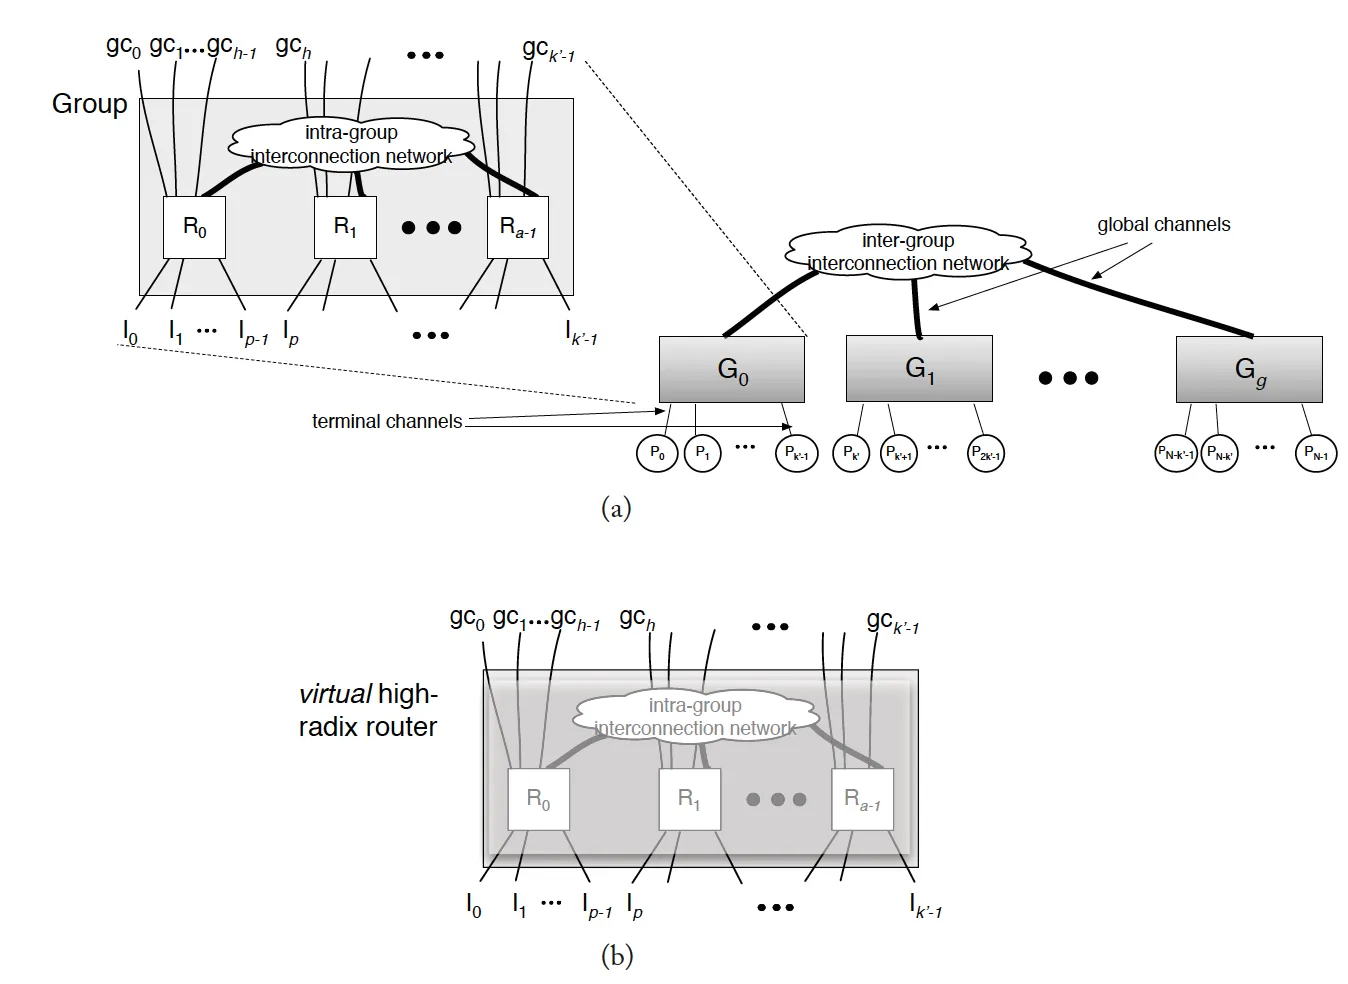
\includegraphics[width=0.8\textwidth]{../assets/ch03/ch03-3_1_网络拓扑-006.png}
\end{figure}
图4.6(b)所示），从而利用输入/输出端口共址的流量局部
性。
然而，Clos或折叠Clos网络的成本几乎是同等容量的蝶形网络的两倍，且延迟更高。成本和延迟的增加
源于数据包需要先路由到任意中间级交换机，再到达最终目的地。这使得网络中的长电缆数量翻倍（成
本约翻倍），并导致穿越的路由器间通道数量翻倍（延迟增加）。
\subsubsection{案例研究：Google Jupiter的演进——从Clos到光交换}

谷歌的数据中心网络架构Jupiter的十年演进，生动展示了Clos拓扑在实际部署中的优势与挑战。2015年，谷歌在SIGCOMM论文中首次披露Jupiter架构，利用商用交换芯片构建五级Clos拓扑，实现了1.3 Pb/s的对分带宽，支持搜索、视频和存储业务的海量需求。

然而，随着规模扩大，Clos拓扑的固有挑战凸显：物理布线复杂性、spine层交换机的高昂成本，以及静态拓扑难以适应动态流量。2022年，谷歌在Jupiter架构中引入了革命性的变革：基于微机电系统（MEMS）的光电路交换机（OCS）。

\textbf{OCS的核心创新}在于将网络拓扑从静态的电域Clos转变为\textbf{动态可重构的直接连接拓扑}。通过OCS，谷歌能够在聚合块之间直接建立光路径，消除了昂贵的spine层电交换机。实际部署表明，这种架构实现了约40\%的功耗降低和30\%的资本支出减少。更重要的是，这种拓扑工程与流量工程的结合，使谷歌能够在不中断业务的情况下实现跨代硬件的平滑升级——这是对传统Clos架构僵化性的根本突破。

谷歌的实践表明，未来的数据中心网络将是"光电混合"的实体：电交换提供细粒度的包级转发，光交换提供大容量的电路级连接。这种融合架构将在AI时代变得愈发重要。

蜻蜓（Dragonfly）拓扑代表了直连网络的最前沿发展，它采用层次化分组设计来优化全局通信。网络被
划分为多个组（Group），组内采用全连接或高维网格，组间则通过稀疏连接形成上层网络。这种结构的
神奇之处在于仅需O(√N)的全局直径，却只需要每个节点3-4个物理端口。美国阿贡国家实验室的"极

                                                            5
光"超算就采用该拓扑，其核心创新在于虚拟通道技术与自适应路由算法的结合，能有效避免热点组间链
路拥塞。




(a) High-level block diagram of dragonfly topology and (b) a virtual high-radix router.
蜻蜓是一种三级分层网络：路由器级、组级和系统级（如上图）。底层每个路由器有三种连接：1)连接到
p个终端；2)通过a−1条本地通道连接到同组其他路由器；3)通过h条全局通道连接到其他组的路由器。因
此，每个路由器的基数（或度数）为k=p+a+h−1。一个组由a个路由器通过本地通道形成的组内互联网络
组成。每组有ap个终端连接和ah个全局通道连接，组内所有路由器共同充当基数为k'=a(p+h)的虚拟路由
器。如上图(b)所示，若忽略组内细节，一个组可视为一个超高基数虚拟路由器（k'>>k）。这种超高基数
使系统级网络能以极低的全局直径（任意两节点间最短路径上昂贵全局通道的最大数量）实现。最多可
连接g=ah+1个组（N=ap(ah+1)个终端），全局直径为1。相比之下，直接用基数k路由器构建的系统级网
络需要更大的全局直径。
在最大规模（N=ap(ah+1)）的蜻蜓网络中，每组间恰好有一条连接。在较小规模的蜻蜓中，每组的全局
连接数超过其他组数量。这些多余的全局连接会均匀分配到各组，确保每组间至少有⌊(ah+1)/g⌋条通
道。蜻蜓参数a、p和h可任意取值，但为在负载均衡流量下平衡通道负载，应满足a=2p=2h。由于每个数
据包在路由中会穿越两条本地通道（全局通道两端各一条）、一条全局通道和一条终端通道，这一比例
能维持平衡。蜻蜓拓扑的路由和负载均衡细节将在第5章讨论。由于全局通道成本高，若偏离2:1的比例，
应超额配置本地和终端通道，以确保昂贵的全局通道充分利用。即网络应满足a≥2h且2p≥2h。通过提高
有效基数，蜻蜓拓扑具有高度可扩展性——使用基数64路由器时，拓扑可扩展至超过256k节点，网络直
径仅为三跳。相比之下，使用基数64路由器的二维扁平化蝶形网络最多扩展至约10k节点，三维版本仅能
扩展至64k节点。

超立方体（hypercube）如图所示，网络中的每个节点可视为一个二进制数。仅有一位数字不同的节点
相互连接。更具体地说，如果两个节点在第 i 位数字上存在差异，则它们在第i维度上相连。在超立方体

                                                                                     6
中，当源节点与目标节点在每个维度上都不同时（例如从图中的000跳转到111），最小路由最多需要
n   跳。然而平均而言，数据包将经历 n/2 跳。




超立方体扩展（HyperX）拓扑扩展了扁平化蝶形，形成更通用的拓扑类别。与扁平化蝶形类似，HyperX
中每维的所有路由器均与同维其他节点全连接，但允许不同维度的交换机数量不同。下图展示了一个
HyperX拓扑示例（L=2维，每维交换机数S1=2、S2=4，集中度T=4，即每个交换机连接4个终端）。定
义HyperX拓扑的另一参数是K，表示每维通道的相对带宽（以终端带宽为单位）。图中假设K=1（所有通
道带宽相等），但若K=2，交换机间通道带宽将是终端通道的2倍。HyperX拓扑可通过四个参数
（L,S,K,T）描述，其中S和K在各维可取值相同（如S1=S2=…=s）形成规则HyperX，或取值不同形成不
规则HyperX。例如，n维超立方体可描述为（L=n,S=2,K=1,T=1），k元n维扁平化蝶形可描述为
（L=n,T=S=k,K=2）。




                                                       7
8


[新增-2026-03] 数据中心网络拓扑

云计算数据中心的网络拓扑与传统企业网络有显著不同。传统数据中心网络主要承载客户机/服务器模式的应用服务，一般采用2层或3层的树形结构（核心层、汇聚层、接入层）。然而，这种传统树形层次结构存在多方面局限性：所有服务器位于同一个2层广播域中；汇聚和核心交换机是服务器之间通信的带宽瓶颈；易于发生"单点故障"。

随着云计算的发展，数据中心网络需要支持：
 ● 超大规模：计算节点数量达到10^5以上量级，交换节点接近10^4量级
 ● 高带宽：服务器之间需要多条通信路径，对分带宽需求巨大
 ● 东西流量主导：数据中心内部流量（东西向）远超进出流量（南北向），比例可达3:1甚至更高
 ● 虚拟机动态迁移：支持VMotion等技术的网络连通性需求

因此，现代数据中心网络拓扑主要采用以下设计：

[新增-2026-03] Fat-Tree拓扑

Fat-Tree是对传统树形层次结构的优化，由Al-Fares等人提出。它仍然分为核心、汇聚和接入3个层次，但具有以下独特之处：

 ● 采用大量统一的廉价商业交换机作为转发设备，避免纵向扩展的高成本
 ● 所有汇聚和接入交换机被划分为不同的集群Pod（k/2台汇聚交换机、k/2台接入交换机），集群内采用全相连方式
 ● 采用多路径路由技术，为服务器之间通信提供较大的对分带宽

Fat-Tree网络中，为实现多路径通信，采用特定的地址分配规则和两级路由表机制。假设使用10.0.0.0/8地址块，Pod内交换机地址形式为10.pod.switch.1，核心交换机地址形式为10.k.j.i，服务器地址形式为10.pod.switch.ID。

[新增-2026-03] Facebook数据中心架构

对于社交网络等特定应用，数据中心的东西流量远超南北流量（可能超出近1000倍）。Fat-Tree结构在这种情况下存在局限性：纵向扩展成本高；昂贵转发设备仍无法有效支撑。

Facebook数据中心采用新型网络结构：
 ● 全面部署廉价架顶交换机（TOR）
 ● 每台架顶交换机以40GBps上行链路与光纤交换机相连
 ● 设计4个相互独立的Spine交换机平面（每个平面可扩展至48台设备）
 ● 集群Pod和骨干平面Spine Plane组成模块化网络拓扑

这种结构通过增加Server Pod实现数据中心扩展，通过增加Spine Plane增加服务器间通信对分带宽。

[新增-2026-03] 无线数据中心网络

随着网络规模扩大，传统有线静态链路面临挑战：布线复杂、难以应对突发流量、改动成本高。无线通信技术为这些问题提供新思路。

60GHz无线通信技术：
 ● 拥有近7GHz宽的可用频谱，可提供Gbps量级速度
 ● 具有抗干扰、防监听特性
 ● 采用有向天线技术、波束成形和波束转向优化链路
 ● 3D-beamforming技术采用反射点到点形式，避免视线链路受障碍物阻塞

自由空间光通信（FSO）：使用可调制的可见或红外光束在自由空间传输，实现更大范围高速传输，避免信号干扰。

[新增-2026-03] 非规则网络结构

REWIRE是针对数据中心网络架构设计的框架，通过优化算法设计无组织、非规则的网络结构：
 ● 在满足用户自定义约束的同时实现最大对分带宽
 ● 最小化端到端延迟
 ● 适用于在现有数据中心基础上进行扩展的场景

REWIRE优化算法分为4步：确定满足约束的网络结构空间；随机选取候选结构；执行local search优化；循环直至找到近似最优结构。

\section{万卡集群的网络拓扑}

随着AI大模型训练规模的指数级增长，单一数据中心的GPU集群已从千卡级别迈向万卡甚至十万卡级别。构建如此规模的训练网络，不仅需要解决单机房的网络架构问题，更需要面对跨机房、跨区域的超大规模互联挑战。本节介绍面向万卡级AI集群的网络拓扑设计。

\subsection{BAG（Backend Aggregation）架构}

BAG（Backend Aggregation，后端聚合）是Meta在其Prometheus等吉瓦级AI集群中采用的核心网络架构技术。它作为集中式的以太网超级汇聚层（Super Spine），负责互联多个Spine层网络，实现跨数据中心和区域的GPU资源池化。

\subsubsection{BAG的定位与功能}

在大型AI集群的分层网络架构中，BAG位于关键的战略位置：

\begin{itemize}
    \item \textbf{区域互联枢纽}：BAG层作为区域网络与主干网络的汇聚点，将分布在多个数据中心的L2网络互联成统一的超级集群
    \item \textbf{容量聚合}：支持Petabit级别的互联带宽（例如，每对区域之间可达16-48 Pbps）
    \item \textbf{统一资源视图}：通过BAG互联，不同物理位置的GPU对上层应用呈现为统一的计算资源池
\end{itemize}

\subsubsection{平面拓扑与分布式拓扑}

BAG层在物理部署上采用分布式架构，以适应大规模集群的需求：

\textbf{平面连接拓扑（Planar Topology）}：BAG交换机在不同区域之间按平面一一对应连接。这种拓扑管理简单，但潜在故障域较为集中。

\textbf{分布式连接拓扑（Spread Connection Topology）}：将链路分散到多个BAG交换机和平面中，提供更丰富的路径多样性和更高的可靠性。当某个BAG交换机或链路故障时，流量可以迅速切换到其他可用路径。

\subsection{跨区域数据中心互联}

BAG架构的核心价值在于支持跨区域的超大规模GPU互联。以Meta的Prometheus集群为例：

\subsubsection{分层互联模型}

\begin{enumerate}
    \item \textbf{建筑内互联}：通过DSF L2网络实现单个建筑内数千GPU的互联
    \item \textbf{区域内互联}：通过BAG层将同一区域的多个建筑互联，形成L3域
    \item \textbf{跨区域互联}：通过BAG-to-BAG连接实现地理分散的数据中心资源的统一调度
\end{enumerate}

\subsubsection{距离与延迟考量}

BAG的分布式架构设计充分考虑了延迟约束：

\begin{itemize}
    \item BAG层与L2边缘之间的距离保持较短，这对于浅缓冲区的NSF（Non-Scheduled Fabric）交换机尤为重要
    \item BAG-to-BAG之间的长距离链路需要采用深缓冲区交换机，以支持PFC等无损拥塞控制协议
    \item 通过优化光纤路由和传输设备，将跨区域延迟控制在RDMA通信可接受的范围内
\end{itemize}

\subsection{多级Clos网络与超配比设计}

万卡级集群的网络拓扑通常采用多级Clos架构的变体，并在不同层级采用差异化的超配比（Oversubscription Ratio）设计。

\subsubsection{三级Clos与超配比}

在典型的万卡集群中，网络通常采用三级架构：

\begin{enumerate}
    \item \textbf{L1层（ToR到Leaf）}：通常采用1:1的无阻塞设计，确保服务器到网络的第一跳带宽充足
    \item \textbf{L2层（Leaf到Spine）}：根据流量模型采用适度的超配比，典型值为4.5:1
    \item \textbf{L3层（Spine到BAG）}：由于跨区域流量相对较小，可以采用更高的超配比（如4.98:1），以降低成本
\end{enumerate}

超配比的选择基于AI训练流量的特征：在数据并行和模型并行训练中，大部分通信发生在同一节点组内，跨区域流量相对有限。因此，适度的高超配比可以在不明显影响性能的情况下显著降低网络成本。

\subsubsection{路由与负载均衡}

BAG架构采用eBGP作为路由协议，并引入链路带宽属性实现UCMP（Unequal Cost Multipath，不等价多路径）：

\begin{itemize}
    \item 根据链路实际带宽进行加权负载分担
    \item 支持动态适应链路故障和带宽变化
    \item BAG-to-BAG连接采用MACsec加密，满足网络安全要求
\end{itemize}

\subsection{混合Fabric架构}

在实际部署中，大型AI集群往往同时采用多种Fabric技术：

\textbf{DSF与NSF的融合}：Meta的Prometheus集群同时部署了DSF（Disaggregated Scheduled Fabric）和NSF（Non-Scheduled Fabric）两种网络：
\begin{itemize}
    \item DSF用于需要高性能、无损传输的训练网络
    \item NSF用于对延迟要求相对宽松的其他后端流量
\end{itemize}

BAG层作为统一的汇聚点，将不同类型的L2网络无缝互联。这种混合架构允许根据具体应用场景选择最合适的网络技术，实现性能与成本的最佳平衡。

\subsection{网络可靠性设计}

万卡级集群的网络可靠性设计需要在多个层面进行考量：

\textbf{故障域分析}：在BAG、数据大厅和电力分配等多个层面进行全面的故障模式分析，确保单点故障不会影响整体训练任务。

\textbf{黑洞避免}：采用多种策略防止路由黑洞，包括：
\begin{itemize}
    \item 受影响的BAG平面流量排空（Draining）
    \item 条件性路由聚合，避免汇聚后的路由震荡
    \item 快速故障检测和路由收敛机制
\end{itemize}

\textbf{增量扩展}：BAG架构支持集群的渐进式扩展。随着AI模型规模的增长，可以通过增加BAG节点和互联链路逐步扩展网络容量，而无需对现有架构进行大规模改造。

\section{[新增-2026-03] AI计算网络创新拓扑}

随着AI大模型训练规模的快速增长，传统数据中心网络拓扑面临成本高、扩展性受限等挑战。华为研究团队在计算网络拓扑领域进行了深入探索，提出了一系列面向AI场景的创新拓扑结构。本节介绍HammingMesh、KNS、Slim Fly和PolarFly四种前沿拓扑，它们在成本、性能和扩展性方面各具特色。

\subsection{HammingMesh拓扑}

HammingMesh是一种专为AI计算集群设计的分层网络拓扑，其核心思想是结合低成本本地互联与高扩展性全局拓扑。该拓扑采用双层架构：本地组（Local Group）使用2D mesh结构，全局层使用Clos拓扑。

\textbf{拓扑参数定义}：HammingMesh由四元组$(a,b,x,y)$定义，其中：
\begin{itemize}
    \item $(a,b)$：本地2D mesh的维度，即每个本地组包含$a \times b$个计算节点
    \item $(x,y)$：全局2D Clos网络的维度
\end{itemize}

\textbf{核心特点}：
\begin{enumerate}
    \item \textbf{低成本本地互联}：本地组内采用PCB铜线直接连接计算芯片，无需昂贵的光模块和交换机，显著降低硬件成本
    \item \textbf{分层解耦设计}：本地通信与全局通信物理分离，本地流量不占用全局网络带宽
    \item \textbf{可扩展全局架构}：利用成熟的Clos拓扑实现全局高对分带宽
\end{enumerate}

\textbf{性能与成本分析}：
\begin{itemize}
    \item All-to-all性能约为同等规模Clos网络的20\%
    \item 相比Dragonfly拓扑成本降低50\%
    \item 相比Clos网络成本降低80\%
\end{itemize}

HammingMesh适用于以本地通信为主、对全局all-to-all性能要求不极致的AI训练场景，如数据并行和流水线并行训练。

\subsection{KNS拓扑}

KNS（K-ary n-dimensional Switched network）拓扑与HammingMesh设计理念相似，但在本地组互联方式上有所区别。KNS在本地组内部使用交换机进行互联，而非直接PCB连接，全局层采用n维Clos拓扑。

\textbf{拓扑特点}：
\begin{itemize}
    \item 本地组通过交换机互联，提供比PCB直连更高的灵活性
    \item 支持n维Clos全局拓扑，扩展性优于2D结构
    \item 2D KNS成本约为Clos网络的40\%
    \item 对分带宽为Clos的一半，all-to-all性能约为50\%
\end{itemize}

KNS在成本和性能之间取得了更好的平衡，适合需要中等全局通信能力的AI训练场景。

\subsection{Slim Fly拓扑}

Slim Fly是一种基于数学图论优化的高效率拓扑，其核心创新在于利用MMS（McKay-Miller-\v{S}ir\'{a}\v{n}）图构建网络结构，达到接近Moore bound的理论极限。

\textbf{理论基础}：
\begin{itemize}
    \item 基于MMS图构建，该图是已知的最大度数为k、直径为2的图类
    \item 达到Moore bound的$\frac{8}{9}$，接近理论最优
    \item 相比同规模Clos网络，可使用更小基数的交换机实现非阻塞特性
\end{itemize}

\textbf{性能优势}：
\begin{enumerate}
    \item 网络直径仅为2跳，延迟极低
    \item 交换机基数需求小，降低硬件成本和功耗
    \item 路径多样性丰富，支持自适应路由
\end{enumerate}

Slim Fly拓扑特别适合对延迟极度敏感的AI推理场景和小规模高速互联场景。

\subsection{PolarFly拓扑}

PolarFly是另一种基于数学图论的前沿拓扑，采用ER（Erd\H{o}s-R\'{e}nyi）极性图作为构建基础。

\textbf{核心特性}：
\begin{itemize}
    \item 基于ER极性图构建，具有优良的对称性和扩展性
    \item 渐进接近Moore bound，在大规模部署时性能优势更加明显
    \item 支持灵活的端口配置，适配不同规模集群需求
\end{itemize}

\subsection{创新拓扑对比分析}

表~\ref{tab:topology_comparison}对上述创新拓扑进行了综合对比：

\begin{table}[htbp]
\centering
\caption{AI计算网络创新拓扑对比}
\label{tab:topology_comparison}
\begin{tabular}{|l|c|c|c|c|c|}
\hline
\textbf{拓扑类型} & \textbf{成本(相对Clos)} & \textbf{对分带宽} & \textbf{All-to-all性能} & \textbf{网络直径} & \textbf{适用场景} \\
\hline
Clos（基准） & 100\% & 100\% & 100\% & $2\log_k N$ & 通用高性能计算 \\
\hline
HammingMesh & 20\% & 中等 & 20\% & 本地1跳+全局多跳 & 数据并行训练 \\
\hline
KNS（2D） & 40\% & 50\% & 50\% & 本地2跳+全局多跳 & 混合并行训练 \\
\hline
Slim Fly & 60\% & 80\% & 85\% & 2 & 低延迟推理 \\
\hline
PolarFly & 55\% & 85\% & 90\% & 2-3 & 大规模训练 \\
\hline
Dragonfly & 40\% & 70\% & 75\% & 3 & 超算中心 \\
\hline
\end{tabular}
\end{table}

从表中可以看出，不同拓扑在成本-性能权衡方面各有侧重。HammingMesh以最低成本满足基本互联需求，Slim Fly和PolarFly则在保持较高性能的同时显著降低成本，为AI基础设施建设提供了更多选择。

\section{[新增-2026-03] 软件定义光电网络}

随着AI模型规模指数级增长，传统电交换网络面临功耗、带宽和灵活性等多重挑战。软件定义光电网络（HyperTPE）通过光交叉连接（OXC）技术和智能控制算法，为超大规模AI集群提供了高效、灵活的网络解决方案。

\subsection{OXC光交叉连接技术}

OXC（Optical Cross Connect，光交叉连接）是软件定义光电网络的核心设备，能够在光层实现灵活的信号路由和调度。

\textbf{OXC技术特点}：
\begin{itemize}
    \item \textbf{全光交换}：光信号直接在光域完成交换，无需光电转换，大幅降低功耗和延迟
    \item \textbf{大容量调度}：单台OXC设备可支持数百端口的全互联，满足超大规模集群需求
    \item \textbf{快速重配置}：通过软件控制实现毫秒级光路切换，支持动态拓扑调整
    \item \textbf{波长级粒度}：支持波长选择性交换，实现精细化的带宽分配
\end{itemize}

\subsection{HyperTPE架构}

HyperTPE（Hybrid Programmable Terabit-scale Photonic-Electronic network）是华为提出的软件定义光电融合网络架构。

\textbf{架构层次}：
\begin{enumerate}
    \item \textbf{光电融合交换层}：OXC负责长距离、大带宽的光路连接，电交换机处理短距离、细粒度流量
    \item \textbf{智能控制层}：集中式控制器统一管理光路和电路资源
    \item \textbf{应用接口层}：提供北向API，支持AI训练框架对网络资源的按需调用
\end{enumerate}

\subsection{拓扑动态重构算法}

HyperTPE的核心能力在于根据AI训练流量特征动态重构网络拓扑。

\textbf{BvN矩阵分解算法}：
基于Birkhoff-von Neumann定理，将流量矩阵分解为多个置换矩阵的凸组合：
\begin{equation}
    T = \sum_{i=1}^{k} \alpha_i P_i, \quad \sum_{i=1}^{k} \alpha_i = 1
\end{equation}
其中$T$为流量矩阵，$P_i$为置换矩阵，$\alpha_i$为权重系数。该分解结果可直接映射为光拓扑配置。

\textbf{贪心流量分配算法}：
对于粗粒度流量分配，采用贪心算法进行优化：
\begin{enumerate}
    \item 按流量大小对通信对排序
    \item 优先为流量大的通信对分配专用光路
    \item 剩余流量通过电交换网络承载
\end{enumerate}

\textbf{拓扑重配置优化模型}：
建立混合整数线性规划（MILP）模型求解最优拓扑：
\begin{align}
    \min_{x,y} \quad & \sum_{i,j} c_{ij}x_{ij} + \lambda \sum_{i,j,k} d_{ijk}y_{ijk} \\
    \text{s.t.} \quad & \sum_{k} y_{ijk} \geq t_{ij}, \quad \forall i,j \\
    & x_{ij} \in \{0,1\}, \quad y_{ijk} \geq 0
\end{align}
其中$x_{ij}$表示光路配置决策，$y_{ijk}$表示流量分配，$t_{ij}$为流量需求。

\textbf{性能指标}：
\begin{itemize}
    \item 256 Pod规模网络：分钟级拓扑计算
    \item 重配置时间减少30\%
    \item 整体网络利用率提升25\%
\end{itemize}

软件定义光电网络为AI大模型训练提供了灵活高效的网络基础设施，代表了数据中心网络演进的重要方向。


\section{蜂窝网络}
% 来源: 19c9fbc4-f642-8f55-8000-0000da7cd9ab_3.1.1_蜂窝网络.pdf
% 提取时间: 2026-02-28T22:51:50+08:00

3.1.1 蜂窝网络
以下是关于蜂窝网的教科书式介绍，内容涵盖组网原理、关键技术及代际演进：


一、蜂窝网的基本概念与组网原理
（一）核心定义
蜂窝网（Cellular Network）是一种采用蜂窝状小区划分的无线通信网络，通过将地理区域划分为多个六
边形小区（类似蜂窝结构），每个小区配备基站（Base Station），实现对用户设备的无线覆盖和通信
服务。其核心思想是利用频率复用技术，在有限的频谱资源下最大化网络容量。
（二）组网架构
1.   小区（Cell）
      ○ 基本覆盖单元，典型形状为六边形（理论上覆盖效率最优），半径通常为几百米到数千米，根
        据地形和用户密度调整。
      ○ 分为宏小区（Macro Cell）（覆盖范围大，用于广域覆盖）、微小区（Micro Cell）（覆盖范
        围较小，用于热点区域）、皮小区（Pico Cell）和飞小区（Femto Cell）（覆盖范围更小，用
        于室内或家庭场景）。
        ■ 微基站（Micro BS）：覆盖半径约 200 米～1 公里，用于中等密度区域（如城区街
          道）。
        ■ 皮基站（Pico BS）：覆盖半径约 50 米～200 米，用于室内或高密度热点（如写字
          楼、购物中心）。
        ■ 飞基站（Femto BS）：覆盖半径约 10 米～50 米，用于家庭或企业小型局域网。




                                                          1
小区分裂（Cell Splitting）是蜂窝网中通过缩小小区半径、增加基站数量来提升网络容量的关键
技术。其核心原理是：在用户密度高的区域将原有的大尺寸小区（如宏小区）划分为多个更小的小
区（如微小区或皮小区），通过缩短基站与用户的距离和增加频率复用次数，在不新增频谱资源的
前提下，提升单位面积内的通信容量和用户服务质量。




     ○ 原小区的频率复用因子为 N（如 7 小区复用模式，N=7），分裂后子小区的覆盖半径缩
       小，同频小区间的距离缩短。为避免同频干扰，需降低频率复用因子（如 N=3 或
       N=1），使相同频率可在更邻近的小区中重复使用，从而提升频谱效率。
     ○ 例：若原小区半径为 R，同频小区间距为 D=3NR；分裂后子小区半径为 R/2，若 N 减
       半，则同频间距 D′=3N/2(R/2)≈D/2，仍需确保 D′ 大于最小干扰距离。
     ○

2. 基站（BS，Base Station）
    ○ 每个小区配备至少一个基站，负责与小区内的用户设备（UE，User Equipment）进行无线信号
      传输，完成信号的调制、解调、编码和解码等功能。
    ○ 早期基站称为BTS（Base Transceiver Station），现代基站（如5G的gNB）集成更多智能化
      功能。
3. 核心网（Core Network, CN）
    ○ 负责处理用户数据、信令交互、移动性管理、鉴权认证等核心功能，通过传输网络（如光纤）



                                                             2
       与基站连接。
     ○ 传统核心网分为电路交换（CS）和分组交换（PS）模块，现代核心网（如5G）采用服务化架
       构（SBA，Service-Based Architecture），实现功能模块化和灵活扩展。
 4. 频率复用（Frequency Reuse）
     ○ 相邻小区使用不同频率，非相邻小区可重复使用相同频率，以提高频谱利用率。例如，7小区复
       用模式中，每个频率组在间隔6个小区后重复使用。


二、蜂窝网关键技术
（一）多址接入技术（Multiple Access Technology）
 ● 频分多址（FDMA，Frequency Division Multiple Access）：将频段划分为多个子信道，用户在频
   域上占用独立信道（如1G的AMPS系统）。
 ● 时分多址（TDMA，Time Division Multiple Access）：将时间划分为时隙，用户在时域上分时共
   享信道（如2G的GSM系统）。
 ● 码分多址（CDMA，Code Division Multiple Access）：为每个用户分配唯一扩频码，通过码型区
   分用户（如3G的WCDMA和CDMA2000系统）。
 ● 正交频分多址（OFDMA，Orthogonal Frequency Division Multiple Access）：将频段划分为正
   交子载波，支持频域资源动态分配（如4G LTE和5G NR系统）。
（二）调制与编码技术
 ● 调制技术：提高频谱效率，如2G的GMSK、3G的QPSK、4G的64QAM、5G的256QAM。
 ● 信道编码：增强抗干扰能力，如卷积码（Convolutional Code）、Turbo码（3G/4G）、低密度奇
   偶校验码（LDPC，5G）和极化码（Polar Code，5G控制信道）。
（三）移动性管理技术
 ● 越区切换（Handover）：用户移动时，通信链路从一个基站切换到另一个基站，分为硬切换（先断
   开原连接再建立新连接，如CDMA系统）和软切换（先建立新连接再断开原连接，如WCDMA系
   统）。
 ● 位置管理：通过位置区（LA，Location Area）和跟踪区（TA，Tracking Area）记录用户位置，支
   持寻呼（Paging）和路由功能。
（四）干扰控制技术
                                                                     3
 ● 功率控制：动态调整基站和用户设备的发射功率，减少小区内和小区间干扰（如CDMA系统的闭环
   功率控制）。
 ● 小区间干扰协调（ICIC，Inter-Cell Interference Coordination）：通过调度资源分配（如频率/时
   隙隔离）降低相邻小区干扰（4G LTE关键技术）。
 ● 波束赋形（Beamforming）：利用多天线技术形成定向波束，增强目标用户信号强度，抑制非目标
   方向干扰（5G NR的Massive MIMO技术）。
（五）双工技术
 ● 频分双工（FDD，Frequency Division Duplex）：上下行通信使用不同频段（如LTE FDD）。
 ● 时分双工（TDD，Time Division Duplex）：上下行通信分时共享同一频段（如LTE TDD和5G NR
   TDD）。


三、蜂窝网的代际演进
蜂窝网技术以“代”（Generation）为单位迭代，每一代均显著提升传输速率、容量和时延性能，下表为
各代技术的核心特征：
 代际      名称           标准化时间 核心技术       典型速率        主要应用场景
 1G      第一代模拟通 1980年代       FDMA、模拟 2.4 kbps      语音通话
         信                   调制（FM）
 2G      第二代数字通 1990年代       TDMA/CDM 9.6 kbps - 语音、短信、
         信                   A、数字调制 14.4 kbps      低速数据
                             （GMSK/QP
                             SK）
 2.5G    GPRS/EDGE 中期        分组交换技术 最高384          网页浏览、彩
                             （GPRS） kbps           信
 3G      第三代移动通 2000年代       CDMA、     2 Mbps - 21 视频通话、移
         信                   WCDMA/CD Mbps         动互联网
                             MA2000/TD
                             -SCDMA



                                                                   4
4G        LTE/LTE-A   2010年代
                          OFDMA、    100 Mbps - 1 高清视频、移
                          MIMO、载波   Gbps         动宽带
                          聚合（CA）
5G        第五代移动通 2019年商用 NR（新空      1 Gbps - 10   物联网、自动
          信               口）、       Gbps          驾驶、
                          Massive                 VR/AR、工业
                          MIMO、毫米                 互联网
                          波、网络切片
6G        第六代移动通 研发中（预计 AI与通信融      理论超100        全域无缝通
          信      2030年商用） 合、太赫兹通    Gbps          信、智能泛在
                          信、空天地海                  服务
                          一体化网络
第一代模拟系统
采用模以下从技术架构、关键技术演进及代际特征角度，对蜂窝网组网技术的演进过程进行专业化阐
述，涵盖从1G到5G的核心变革与技术突破：


一、模拟蜂窝网时代（1G，1970s-1980s）：频分多址与孤立小区组网
技术架构核心
●   单小区覆盖模型：
  采用**宏小区（Macro Cell）**架构，单个基站覆盖半径5-15公里，信号通过全向天线或定
  向天线（扇形分区，如3扇区）辐射。
● 频分多址（FDMA）技术：

   ○ 频段划分：将可用频谱划分为互不重叠的窄带信道（如AMPS系统带宽30kHz/信道，
     TACS系统25kHz/信道），用户通过不同频段实现物理层复用。
   ○ 频率复用机制：采用7小区复用模式（复用因子(N=7)），通过地理上间隔6个小区重用相同
     频段，解决频谱资源有限问题，但受限于同频干扰，容量提升受限。
关键技术局限
●   频谱效率低下：仅支持语音业务，频谱利用率约1-2 bps/Hz，单小区容量仅数十用户。

                                                             5
● 无移动性管理：缺乏越区切换（Handover）机制，用户跨小区需重新拨号，网络连续性差。
● 模拟信号缺陷：易受噪声干扰，保密性差，无法支持数据业务。




二、数字蜂窝网时代（2G，1990s-2000s）：分层组网与信令标准化
组网架构革新
1.   分层小区结构（Heterogeneous Cell Structure）
      ○ 宏小区（Macro Cell）：覆盖郊区及低密度区域，半径1-10公里，支持广域覆盖。

      ○ 微小区（Micro Cell）：部署于城区高密度区域，半径0.5-2公里，分担宏小区话务压力，
        形成宏-微分层网络。
      ○ 小区分裂（Cell Splitting）：通过缩小小区半径（如从10公里降至5公里）并增加基站密
       度，将原小区划分为多个子小区，复用因子(N)不变时容量提升(4倍（面积与半径平方成
       正比）)。
2.   移动性管理架构
      ○ 核心网-接入网分离：

         ■ 基站（BTS）：负责无线信号收发，连接终端（MS）。

         ■ 基站控制器（BSC）：管理多个BTS，执行无线资源分配、越区切换判决（如基于信
           号强度的A3/A5信令）。
         ■ 移动交换中心（MSC）：处理用户呼叫接续、位置登记，跨MSC切换需通过网关MSC
           （GMSC）协调。
      ○ 硬切换（Hard Handover）：先断开原小区连接，再接入新小区，存在短暂通信中断，适
        用于FDMA/TDMA系统（如GSM）。
3.   多址技术升级
      ○ 时分多址（TDMA）：GSM将每个200kHz载波划分为8个时隙（Time Slot），单载波容量
        提升8倍，频谱效率达13 bps/Hz（含信道编码）。
      ○ 码分多址（CDMA，IS-95）：引入正交码分复用（如Walsh码），通过扩频技术实现同频
        复用（复用因子(N=1)），利用功率控制和RAKE接收机抑制多址干扰（MAI），频谱效率
        提升至1.2288 Mcps带宽下约1.5 bps/Hz。
关键技术突破
●    频率复用优化：GSM采用4×3复用模式（(N=4)），结合跳频（Frequency Hopping）降低同频
                                                          6
  干扰，复用因子可进一步降至(N=3)，容量提升50%。
● 信令标准化：定义公共控制信道（CCCH）、专用控制信道（DCCH），实现接入控制、寻
  呼、功率控制等功能的标准化。

三、宽带蜂窝网时代（3G，2000s-2010s）：分组交换与异构网络萌芽
组网架构演进
1.   从电路交换到分组交换
      ○ 核心网IP化：引入分组交换域（PS Domain），支持数据业务（如HSPA下载速率达14.4
        Mbps），与传统电路交换域（CS Domain）并存。
      ○ 无线接入网（RAN）扁平化：UMTS系统中，Node B（基站）通过RNC（无线网络控制
        器）连接核心网，RNC负责切换控制、功率控制等，形成两层架构。
2.   异构网络（Heterogeneous Network, HetNet）雏形
      ○ 微微小区（Pico Cell）：覆盖半径100-500米，部署于室内或热点区域，支持更高数据速
          率。
      ○   小区呼吸（Cell Breathing）：CDMA系统中，通过调整基站发射功率动态改变小区覆盖范
          围，平衡负载（如高负载时缩小覆盖范围，减少干扰）。
3.   切换技术升级
      ○ 软切换（Soft Handover）：CDMA系统中，终端可同时与多个基站建立连接（宏分集），
        实现“先连后断”，降低掉话率，但增加网络信令负荷。
      ○ 接力切换（Batton Handover，TD-SCDMA）：结合硬切换与软切换优势，利用上行同步
        提前获取目标小区参数，减少切换时延。
多址技术与物理层革新
●    正交频分多址（OFDMA，LTE前身技术）：3GPP在HSPA+中引入64QAM调制与MIMO（2×2
  天线），频谱效率提升至30 bps/Hz（20MHz带宽）。
● 智能天线（Smart Antenna）：TD-SCDMA采用8阵元天线阵列，通过波束赋形
  （Beamforming）提升信号强度，抑制干扰，小区边缘速率提升2-3倍。

四、全IP蜂窝网时代（4G/LTE，2010s-2020s）：扁平化架构与干扰协同
                                                            7
组网架构重构
1.   接入网扁平化（Flat RAN）
      ○ 取消RNC节点：LTE中eNodeB（eNB）直接连接核心网（MME/S-GW），实现用户面与
        控制面分离，切换决策由eNB自主完成，时延从数百毫秒降至50ms以下。
      ○ 自组织网络（SON）：eNB通过X2接口自动协调邻区关系，支持自动邻区配置（ANR）、
        干扰协调（ICIC），降低人工运维成本。
2.   超密集异构网络（UDN, Ultra-Dense Network）
      ○ 小小区（Small Cell）大规模部署：引入家庭基站（Femto Cell，覆盖10-100米）、微基站
        （Micro Cell），形成“宏基站+小小区”多层网络，小区密度达10-20个/平方公里，容量
        提升10-20倍。
      ○ 干扰管理技术：
         ■ 部分频率复用（FFR, Fractional Frequency Reuse）：边缘用户使用专用频段，中心用
           户共享全频段，降低跨层干扰。
         ■ 协调多点传输（CoMP, Coordinated Multi-Point）：多个基站联合为同一用户服务，
           提升小区边缘频谱效率（如LTE-A Pro中提升30%）。
3.移动性管理优化
● 基于X2接口的切换：同频切换通过eNB间直接通信完成，时延低于30ms；异频切换由MME协
  助，支持无损切换（GTP-U隧道转发）。
● 载波聚合（CA, Carrier Aggregation）：聚合2-5个载波（最大100MHz带宽），提升峰值速率
  （LTE-A达1Gbps），同时支持跨载波切换。
物理层与多址技术
●    OFDMA上行/下行：下行OFDMA（子载波15kHz）支持频域资源动态分配，上行SC-FDMA
  （单载波频分多址）降低峰均比（PAPR），适合终端发射。
● 大规模MIMO（Massive MIMO）：基站配置64/128阵元天线，通过波束赋形实现空分多址
  （SDMA），单小区容量提升5-10倍，频谱效率达50 bps/Hz（20MHz带宽）。

五、智能蜂窝网时代（5G，2020s-）：分层异构与智能化协同
组网架构革命性突破
1.   空天地海一体化网络（STHA, Space-Air-Ground-Sea Integrated Network）
                                                                8
      ○   低轨卫星（LEO）：补充地面覆盖盲区，如Starlink提供全球宽带接入，时延控制在50ms
          以内。
      ○   无人机基站（UAV/Beehive）：快速部署于应急场景，通过毫米波（如28GHz）与地面基
        站形成临时回传链路。
      ○ 海面基站：采用抗腐蚀天线与长续航设计，覆盖近海区域，支持海事通信与海洋物联网。

2.   超异构网络（Hyper-HetNet）
      ○ 三频组网（Sub-6GHz+毫米波+可见光）：

          ■Sub-6GHz（如3.5GHz）负责广域覆盖与移动性支持；
         ■ 毫米波（24-100GHz）提供短距离超高带宽（单链路速率达10Gbps），用于热点区
           域（如体育场、机场）；
         ■ 可见光通信（VLC）作为补充，在室内通过LED灯实现无射频干扰的数据传输。
      ○ 智能超表面（RIS, Reconfigurable Intelligent Surface）：部署于建筑墙面或基站侧，通过
        数千个无源反射单元动态调控电磁波传播路径，提升小区边缘速率3-5倍，降低穿透损耗
        20dB以上。
3.   分布式单元（DU）与集中式单元（CU）分离
      ○ 云化RAN（C-RAN）：将基站基带处理单元（BBU）集中为CU，射频单元（RRU）作为
        DU分布式部署，通过前传网络（如25G光模块）连接，支持基带资源池共享，降低功耗
        30%以上。
      ○ 边缘计算（MEC, Multi-Access Edge Computing）：在CU或靠近基站的位置部署边缘服
        务器，本地化处理时延敏感业务（如自动驾驶，时延<10ms），减少核心网传输压力。
移动性与干扰管理
●    基于AI的切换决策：利用强化学习（RL）算法，综合信号强度、负载、用户移动轨迹等参数，
     优化切换触发时机，掉话率降低40%。
●    干扰对齐（IA, Interference Alignment）：在毫米波MIMO系统中，通过预编码将多小区干扰信
     号对齐到同一子空间，仅占用1/3维度资源，提升有用信号维度至2/3，频谱效率提升2倍。
多址技术与物理层创新
●    非正交多址（NOMA, Non-Orthogonal Multiple Access）：在功率域复用用户（如强用户与弱
  用户叠加传输），通过串行干扰消除（SIC）分离信号，单小区容量提升50%，适用于物联网
  海量连接场景。
● 太赫兹通信（0.1-10THz）：试验性部署于短距离场景（如芯片间通信、工业传感器网络），带



                                                                    9
    宽达数十GHz，理论速率超100Gbps，但受大气衰减限制，覆盖半径<10米。

六、未来演进方向（6G，2030s预研）
●   太赫兹蜂窝网：探索0.1-10THz频段组网，结合超材料天线实现波束精准控制，支持亚毫米级
    定位与全息通信。
●   基于量子通信的安全组网：引入量子密钥分发（QKD）保障信令安全，量子中继解决长距离密
  钥传输损耗问题。
● 生物启发式网络：模拟蜂巢结构动态调整小区形态，如根据用户密度实时生成“液态小区”，基
  站通过无人机集群或自重构硬件快速部署。

总结：组网演进的核心逻辑
蜂窝网组网技术始终围绕频谱效率提升（从FDMA的1 bps/Hz到5G Massive MIMO的50+
bps/Hz）、覆盖与容量平衡（从单一宏小区到Hyper-HetNet）、移动性增强（从硬切换到AI驱动
的智能切换）三大主线发展，未来将向智能化、空天一体化、太赫兹高频段方向突破，最终实现“泛
在连接、零等待通信、厘米级定位”的终极目标。




                                                   10


\chapter{交换}
% 来源: 19c9fbc3-e182-829e-8000-00002574d509_3.2_交换.pdf
% 提取时间: 2026-02-28T22:51:48+08:00

3.2 交换
电路交换
电路交换（Circuit Switching）是一种通信网络技术，其核心思想是在通信双方之间建立一条专用
的物理通信路径（电路），该路径在通信过程中始终保持连接状态，直到通信结束后才会释放。这
种技术类似于传统电话系统的工作方式，例如拨打固定电话时，电话交换机会在通话双方之间建立
一条独占的物理线路。
工作原理
电路交换的工作过程主要包括以下三个阶段：
1.   建立连接阶段
     ○ 发送方向网络发出连接请求，请求中包含接收方的地址信息。
     ○ 网络通过中间节点（如交换机）逐步建立从发送方到接收方的端到端物理连接，这条线路

       在通信期间由双方独占。
     ○ 示例：传统电话网络中，用户拨号后，交换机通过布线建立通话双方的物理线路。

2.   数据传输阶段
     ○ 连接建立完成后，数据通过这条专用线路进行传输，传输过程中无需进行路由选择，数据
       按顺序直达对方。
     ○ 特点：传输延迟低、数据顺序稳定，但线路利用率可能较低（即使无数据传输，线路也被

       占用）。
3.   连接释放阶段
     ○   通信结束后，双方中的任意一方发起断开请求，网络拆除已建立的物理连接，释放占用的
         线路资源。
电路交换的主要特点
优点                         缺点




                                                   1
1. 传输可靠性高：专用线路避免了其他通信的     1. 线路利用率低：连接建立后即使无数据传
干扰，数据不会丢失或乱序。              输，线路也被独占，资源浪费明显。
2. 延迟固定且低：无需等待路由选择，适合实     2. 灵活性差：无法动态适应数据流量的变化，
时性要求高的业务（如语音通话）。           不适合突发型数据传输（如互联网数据）。
3. 操作简单：通信过程中网络无需处理复杂的     3. 建立连接耗时：需等待线路接通，对短时间
流量控制。                      通信效率较低。

分组交换
分组交换（Packet Switching）是一种基于存储转发机制的通信网络技术，其核心思想是将数据分割成
若干个独立的分组（Packet，也叫数据包），每个分组携带源地址、目的地址等信息，通过网络中的节
点（如路由器）逐跳转发，最终到达目的地。与电路交换不同，分组交换不预先建立专用物理线路，而
是让多个分组在网络中共享带宽资源，动态选择路由路径。
工作原理
1. 数据分割与封装
   ● 发送端将原始数据分割成固定或可变长度的分组（例如IP分组的最大长度约为1500字节）。
   ● 每个分组包含：
      ○ 头部（Header）：源地址、目的地址、分组序号、校验信息等控制信息。
      ○ 载荷（Payload）：实际数据内容。

2. 存储转发与路由选择
   ● 分组通过网络节点（路由器、交换机）传输时，节点会先存储分组，再根据头部的目的地址查找路
     由表，选择下一个转发节点。
   ● 关键特点：
      ○ 不同分组可能通过不同路径到达目的地（如A→B→D和A→C→D两条路径）。
      ○ 无需预先建立连接，网络资源按需分配。

3. 重组与交付
   ● 接收端收到所有分组后，根据分组序号重新组装成完整数据，并校验数据完整性。
   ● 若分组丢失或出错，通过反馈机制请求重传（如TCP协议的确认机制）。


分组交换的主要特点

                                                        2
优点                        缺点
1. 资源利用率高：多个用户共享网络带宽，避免   1. 传输延迟不确定：分组可能因路由拥堵而排
电路交换的“闲置占用”问题。            队，导致延迟波动（实时性较差）。
2. 灵活性强：动态路由适应网络拓扑变化，支持   2. 分组开销：头部信息增加了额外数据量（例如
突发数据传输（如网页浏览、文件下载）。       IP分组头部占20~60字节）。
3. 成本低：无需为每个通信预分配专用线路，适   3. 数据可能乱序：不同分组路径不同，需接收端
合大规模数据网络（如互联网）。           重新排序（通过序号解决）。

分组交换的分类
根据分组处理方式，可分为两类：
1. 数据报交换（Datagram Switching）
  ● 无连接服务：每个分组独立路由，互不关联。

2. 虚电路交换（Virtual Circuit Switching）
  ● 面向连接服务：通信前先建立一条逻辑连接（虚电路），所有分组沿同一路径传输。




数据报交换

                                                    3
数据报的设计理念非常直接：每个数据包都携带足够的信息，使得任何交换机都能够独立决定如何将其
转发至目标地址。具体来说，每个数据包内含完整的最终目的地地址。为了确定数据包的正确传输路
径，交换机会依据转发表（亦称为路由表）进行决策。然而，在规模庞大且动态变化复杂的网络环境中
构建转发表则更具挑战性，尤其是在存在多条可能通往同一目的地路径的情况下。这一过程被称为路
由。我们可以将路由视为一种后台运行的过程，确保每当有新的数据包到达时，都有现成的转发表可供
查询，从而指导该数据包的正确转发。
 ● 无连接特性：由于只要转发表正确填充，数据包便能在任意时刻通过任一交换机立即被转发，因此
   这类网络常被视为无连接的。这与后文将讨论的面向连接型网络形成对比，后者需要在实际数据传
   输前建立并维护一定的连接状态。
 ● 不可预见性：发送端无法事先得知其发出的数据包是否能够成功送达目标地址，或目标主机是否处
   于可用状态。
 ● 独立性：即使目的地相同，连续发送的两个数据包也可能选择不同的路径完成传输，这是因为途中
   某交换机的转发表可能发生变动。
 ● 容错能力：面对交换机或链路故障，如果系统能够及时更新转发表，则这些故障不会对整个通信过
   程产生致命影响。这一点对于提升互联网整体稳定性至关重要。
虚电路交换
另一种分组交换技术采用虚拟电路（VC）的概念。此方法也被称为面向连接模型，要求在实际数据传输
前先行建立一条虚拟路径。整个过程可分为两个阶段：“连接建立”和“数据传送”。
在连接建立阶段，需在源主机与目标主机之间所有经过的交换机上创建相应的“连接状态”。对于单个连
接而言，其状态包括每台涉及交换机内的VC表项记录。具体的VC表项包含如下信息：
  ● 虚电路标识符(VCI)：用于唯一识别本交换机处属于该连接的所有数据包；
  ● 入站接口：指定接收到此VC相关数据包的具体端口；
  ● 出站接口：指明此类数据包离开交换机时所使用的出口；
  ● 新VCI值：用于替换原VCI字段的新值。

当数据包抵达指定入口且其头部携带匹配的VCI时，该数据包应被重定向至指定出口，并更新其头部VCI
字段为新值。值得注意的是，VCI加上传入接口共同定义了一条虚拟连接；在同一交换机内部可能存在多
个同时活跃的虚拟连接。此外，通常情况下，进出方向上的VCI并不一致，这意味着VCI仅在其所在链路
上有效（即具有局部意义）。
每当新增一条连接时，必须为其途经的所有链路分配唯一的VCI，并保证该值未被现有活动连接占用。关
于如何建立连接状态有两种常见方式：一是通过网络管理员手动配置，形成的虚拟电路称作永久虚拟电
路(PVC)；二是由终端设备发起请求，通过信令机制自动设置，这样的虚拟电路则称为切换虚拟电路
(SVC)。SVC允许用户动态地建立及拆除连接而无需人工干预。
关于虚拟电路交换，需要注意以下几点：
                                                 4
●  A到B的传输，因为主机A必须等待连接请求到达远端并在可以发送其第一个数据之前返回数据
   包，之前至少有一个往返时间（RTT）延迟发送数据。
 ● 当连接请求包含主机B的完整地址时（它可能非常大，是网络），每个数据包仅包含一个小标
   识符，即只有一个链接是唯一的。因此，由标头相对于数据报模型减少。更重要的是，查找速
   度很快，因为可以处理虚拟电路号作为表的索引，而不是作为必须查找的键向上。
 ● 如果连接中的交换机或链路出现故障，则表示连接断开需要建立一个新的。另外，旧的需要拆
   下以释放交换机中的表存储空间。
 ● 交换机如何决定转发哪个链路的问题上的连接请求已被掩盖。本质上，这是与建立数据报转发
   表相同的问题转发，这需要某种路由算法.路由将在后面的部分中介绍，并且在那里介绍了算
   法通常适用于路由设置请求以及数据报。
虚拟电路最常见的应用是的构造虚拟专用网络（VPN）。
区别电路交换，分组交换的虚电路交换与数据报交换




交换机微结构
为了实现前几章所述的高基数拓扑结构，需要一种能够扩展至高端口数量的可扩展交换机微架构。传统
用于低基数拓扑的路由器微架构端口数量有限（即6至8个端口），因此可采用集中式仲裁。然而，仲裁
                                                 5
逻辑的复杂度与O(k²)成正比，其中k为路由器的基数（输入和输出端口的数量）。本章将描述一种与低
基数路由器[49, 55]类似的基准路由器设计。由于分配器的复杂性以及连接输入和输出端口所需的布线，
该设计难以扩展至高基数。为了克服这一限制并同时提供高性能，我们介绍了一种采用中间缓冲的分层
交换机结构，通过解耦输入和输出的分配，同时减少所需的中间缓冲量。
路由器微架构基础
图1 展示了基准路由器架构的框图。到达的数据存储在输入缓冲区中。这些输入缓冲区通常分为多个并行
的虚拟通道，用于防止死锁、实现优先级分类，并通过允许被阻塞的数据包通过来提高吞吐量。输入缓
冲区和其他路由器资源以固定大小的单元（称为flit）分配，每个数据包被拆分为一个或多个flit，如图2
所示。




图1 Baseline virtual channel router




图2 (a) Packets are broken into one or more flits (b) Example pipeline of flits through the
baseline router

                                                                                             6
数据包在路由器中的传输可分为每包和每flit的步骤。包头flit（数据包的第一个flit）到达时即触发每包操
作：
 1. 路由计算（RC）：根据包头中存储的信息选择数据包的输出端口。
 2. 虚拟通道分配（VA）：数据包必须独占访问与路由计算输出端口关联的下游虚拟通道。完成这些每
    包步骤后，即可开始数据包的每flit调度。
 3. 交换机分配（SA）：如果输出虚拟通道中有空闲缓冲区，flit可以竞争交叉开关的访问权。

 4. 交换机遍历（ST）：一旦flit获得交叉开关访问权，即可从输入缓冲区传输至输出端口并进入下游路
    由器。
这些步骤对数据包的每个flit重复执行，尾flit（数据包的最后一个flit）传输完成后，虚拟通道被释放，可
供其他数据包使用。\begin{figure}[htbp]
\centering
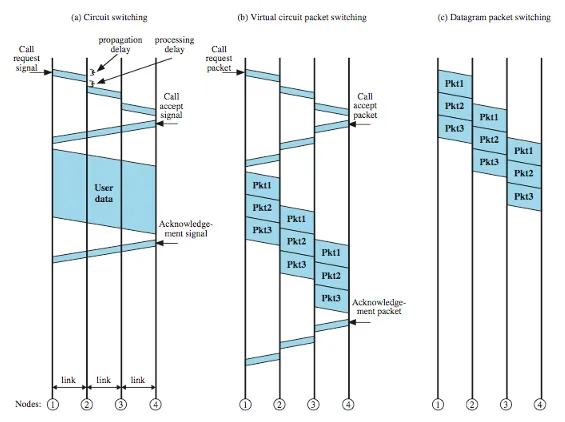
\includegraphics[width=0.8\textwidth]{../assets/ch03/ch03-3_2_交换-002.png}
\end{figure}
图6.2(b)展示了三flit数据包的简单流水线图，假设每个步骤占用一个时钟周期。
将基准微架构扩展至高基数
随着基数增加，集中式分配方法因布线、芯片面积和延迟的急剧增加而变得不可行。本节介绍适用于高
端口数量的分布式交换机和虚拟通道分配结构。
通过采用图3所示的分布式可分离分配器设计，我们解决了交换机分配器的可扩展性问题。分配分为三个
阶段：输入仲裁、本地输出仲裁和全局输出仲裁。第一阶段，每个输入控制器中所有就绪的虚拟通道请
求访问交叉开关。每个输入控制器中获胜的虚拟通道通过驱动请求输出端口的二进制代码到一组水平请
求线上，将请求转发至相应的本地输出仲裁器。




Scalable switch allocator architecture. The input arbiters are localized but the output arbiters are
distributed across the router to limit wiring complexity. A detailed view of the output arbiter
corresponding to output k is shown to the right.
在每个输出仲裁器中，输入请求被解码。第二阶段，每个本地输出仲裁器从其管理的m个输入请求（图
6.3中m=8）中选择一个请求（如有）转发至全局输出仲裁器。最后，全局输出仲裁器从k/m个本地输出

                                                                                                       7
仲裁器中选择一个请求（如有）授予其交换机输出访问权。对于极高基数的路由器，两级输出仲裁器可
扩展至更多级。
分布式仲裁器的每个阶段在相对较少的输入（通常不超过16个）上做出仲裁决策，确保每级可在一个时
钟周期内完成。前两级的仲裁是局部的，仅在物理位置相近的请求中选择。最后一级通过全局布线收集
分布式请求信号，使实际仲裁可在本地执行。确定输出的获胜请求者后，授权信号回传至请求的输入虚
拟通道。为确保公平性，每级仲裁器维护一个基于请求轮转的优先级指针。
虚拟通道分配（VA）比交换机分配更复杂，因为待分配的资源数量乘以虚拟通道数v。与通过信用计数跟
踪下游缓冲区可用性的交换机分配不同，虚拟通道分配中下游虚拟通道的可用性未知。理想的虚拟通道
分配器需允许所有输入虚拟通道监控其等待的所有输出虚拟通道状态，但这种分配器的布线复杂度高达
v²k²，成本过高。
基于交换机分配的设计思路，可构建可扩展的虚拟通道分配器架构。输出虚拟通道的状态保存在每个交
叉点，分配也在交叉点进行。但虚拟通道分配涉及推测，即交换机分配在虚拟通道分配完成前启动以减
少延迟。




图4 Block diagram of a (a) baseline crossbar switch and (b) fully buffered crossbar switch.
全缓冲交叉开关
在交换机的交叉点添加缓冲（图4b）可解耦输入和输出的虚拟通道及交换机分配。这种解耦简化了分
配，减少了对推测的需求，并克服了采用分布式推测分配器的基准架构的性能问题。由于输入和输出交
换机分配完全解耦，赢得输入仲裁的flit会立即转发至其输出对应的交叉点缓冲区。在交叉点，执行与无
缓冲交换机相同的本地和全局输出仲裁。但由于flit已在交叉点缓冲，即使输出仲裁失败也无需重新在输
入端仲裁。

                                                                                             8
中间缓冲区与输入虚拟通道关联。交叉点缓冲区实质上是输入缓冲区针对每个输出的扩展，因此无需为
到达交叉点执行虚拟通道分配——flit已持有输入虚拟通道。输出虚拟通道分配分两步进行：首先通过v选
1仲裁器选择每个交叉点的虚拟通道，再通过k选1仲裁器选择与输出通信的交叉点。
为防止交叉点缓冲区溢出，需采用基于信用的流控。每个输入为其行中的每个kv交叉点缓冲区维护独立
空闲计数器。发送flit至缓冲区时，对应计数器递减；计数为零时，禁止发送。当flit离开交叉点缓冲区
时，返回信用以递增输入的空闲计数。交叉点缓冲区的所需大小由信用延迟（从输入计数器递减到信用
返回的空载交换机延迟）决定。
同一输入行的多个交叉点可能在同周期向不同输出发送flit，从而产生多个信用。高效回传这些信用是一
大挑战。为每个交叉点设置专用信用线成本过高，因此同一输入行的所有交叉点共享一条信用返回总
线。返回信用时，交叉点需仲裁总线访问权。信用返回总线仲裁器采用与输出交换机仲裁器相同的本地-
全局分布式仲裁方法。
在交叉点缓冲区充足的情况下，该设计可实现100%容量饱和吞吐量，因为头部阻塞被完全消除。随着交
叉点缓冲量增加，全缓冲架构逐渐接近虚拟输出队列（VOQ）交换机（每个输入为每个输出维护独立缓
冲区）。全缓冲交叉开关相比VOQ的优势在于无需复杂分配器——6.2节讨论的简单分布式分配方案即可
实现100%吞吐量。
然而，全缓冲交换机的高性能以更大的路由器面积为代价。交叉点缓冲量与vk²成正比，随基数增加成为
芯片面积主导因素。存储面积包括交叉点和输入缓冲区，布线面积包括交叉开关本身及仲裁和信用返回
的控制信号面积。基数增加时，交叉开关带宽（及其面积）保持恒定。布线面积随基数增加源于控制复
杂度的提升。基数超过50时，存储面积超过布线面积。

样例：MELLANOX INFINISCALE IV
InfiniBand协会（ITA）长期制定点对点I/O通信规范，逐步发展为高性能网络结构。InfinisScale IV
（IS4）的链路以2.5Gb/s、5Gb/s和10Gb/s的速率异步运行，宽度可为1x或4x，总链路带宽分别为
10Gb/s（SDR）、20Gb/s（DDR）或40Gb/s（QDR）。




                                                               9
图9 IS4交换芯片的框图，该芯片具有36个端口，每个端口支持4至10 Gb/s，总聚合带宽为2.88 Tb/s的
片外带宽。
IS4微架构采用传统的方法，以非阻塞12×12交叉开关为基本构建块。通过3倍复制形成36端口路由器。
InfiniBand结构中每个主机标有本地标识符（LID），每个交叉开关使用48K条目线性转发表（LFT）通过
目标LID索引路由单播数据包。
多个4x端口可聚合为8x或12x端口，提供每方向40、80或120Gb/s带宽。这使得36端口4x QDR路由器可
视为12端口12x QDR（每方向120Gb/s）路由器，为构建胖树或带网络加速的环面网络提供了灵活性。
每个IS4芯片提供16个服务等级（SL），其中SL15保留给称为管理数据报（MAD）的控制消息。SL在包
头中携带且路由过程中不变。每跳执行服务等级到虚拟通道（VL）的分配。IS4支持最多8个独立VL，可
用于路由算法中的死锁避免、性能隔离或服务质量（QoS）。VL采用基于信用的流控管理下游输入缓冲
区空间，绝不会因输入缓冲区拥塞丢弃数据包，而是阻塞发送端。若其他VL在输入缓冲区中有空间，则
可继续流动。除SL15（管理SL）外，网络链路均采用虚拟直通流控（VCT），硬件不提供流控时由软件
实现。




                                                       10


\section{交换机设计}
% 来源: 19c9fbc3-c752-8f62-8000-00009c915a0b_3.2.1_交换机设计.pdf
% 提取时间: 2026-02-28T22:51:46+08:00

3.2.1 交换机设计
1 交换机
在电话通信中，一次电话连接通常持续数秒甚至数分钟。然而在互联网交换机中，每次连接仅持续一个
数据包的传输时间。对于一个40字节的数据包，在40Gbps的速率下，这个时间是8纳秒。因此，为了以
线速运行，交换系统必须在最短的数据包到达时间内决定（即计算）应该匹配哪些输入和输出链路。这
使得互联网交换机的控制部分（用于建立连接）比电话交换机更难构建。为此，
在数据面，大多数路由器在将可变大小的数据包发送到交换结构之前，会在内部将其分割为固定大小的
信元。
在控制面，根据数据到达情况，交换组件输入输出端口建立连接，可归结为解决一个二分匹配问题：路
由器必须在固定的信元到达时间（时隙）内，尽可能地将输入链路与输出链路进行匹配
1.1 发展历程：从总线到Crossbar




图1 网络交换机的演进，从带有共享CPU的共享总线交换机到每个线路卡带有专用转发引擎的CrossBar
交换机

                                                      1
在介绍基于总线和CrossBar（crossbar）的交换机之前，先了解一种基于共享内存的简单交换机实现方
式是有益的。这种设计的基本原理是：数据包从输入链路进入后被存储到共享内存中，随后从内存读取
并发送到对应的输出链路。这种技术在电话通信中的时隙交换中已有多年应用，同时也适用于小型网络
交换机。
然而，这种设计的主要瓶颈在于内存带宽。假设芯片有8个输入链路和8个输出链路，那么每个数据包需
要经历一次写入和一次读取操作，这意味着内存的运行速度必须达到单链路速度的16倍。为缓解这一问
题，可以通过增加内存访问宽度来优化。例如，输入链路上的串行比特流可以累积到一个移位寄存器
中，当完整的信元累积完成后，将其一次性写入宽字内存。类似地，数据包在读取时也会被加载到输出
移位寄存器中，随后逐位移出到输出链路。
尽管这种共享内存的设计易于在芯片上实现，并可通过流量控制和外部缓冲区扩展，但其扩展性有限。
主要原因是它无法处理超过信元大小的数据包。如果交换机同时收到多个发往不同目的地的小型数据
包，虽然可以将它们打包成一个宽字存储，但无法保证它们能同时被读出。
随着技术发展，交换机已经从简单的共享介质（如总线或共享内存）架构演进到更现代的CrossBar架
构。在早期的共享总线设计中，所有线路卡通过一条高速总线连接，每次只能允许一对线路卡通信。例
如，当线路卡1向线路卡2发送数据包时，其他线路卡之间的通信会被阻塞。此外，在早期路由器中，转
发决策由一个通用CPU负责，这虽然简化了软件设计，但由于通用CPU的低效指令执行和缺乏实时约束
能力，导致性能受限。同时，数据包需要两次经过总线（一次到CPU，一次从CPU到目标），进一步增
加了延迟。
为了缓解CPU瓶颈，后续设计引入了多CPU架构，每个CPU负责一部分线路卡的转发任务。这种方法提
高了吞吐量并降低了单个CPU的性能要求，但也可能引发数据包乱序问题。
尽管如此，共享总线仍然是系统的主要瓶颈。由于总线需要支持多个数据源和目的地，电气负载、信号
上升时间和反射等问题限制了其传输速度。为解决这些问题，CrossBar交换机应运而生。CrossBar交换
机采用一组2N条并行总线（每条源线路卡和目的线路卡各对应一条总线），形成矩阵结构。理论上，这
种设计比单总线架构快N倍，因为在最佳情况下，所有N条总线可以同时传输数据。然而，要充分发挥其
性能潜力，需要解决调度问题，即在每个时隙找到N对不冲突的源-目通信对。这一问题构成了本章研究
的核心内容。
1.2 CrossBar交换结构




                                                    2
图3 基本CrossBar交换机
最简单的CrossBar结构是一个由N条输入总线和N条输出总线组成的阵列，如图3所示。因此，如果线路
卡R希望向线路卡S发送数据，则输入总线R必须连接到输出总线S。实现这种连接的最简单方法是通过一
个“传输”晶体管，如图4所示。对于每一对输入和输出总线，如R和S，都有一个晶体管，当晶体管导通
时，就连接了这两条总线。这样的连接被称为交叉点。请注意，一个具有N个输入和N个输出的CrossBar
交换机有N²个交叉点，每个交叉点都需要一条来自调度器的控制线来控制其导通或关闭。




图4 通过导通连接两条总线的传输晶体管，将来自线路卡R的输入连接到线路卡S。现代CrossBar交换机
用多路复用器树取代了这种简单设计，以降低电容
虽然N²个交叉点看起来数量很多，但通过晶体管进行的超大规模集成电路（VLSI）实现使得引脚数量、
卡连接器技术等成为构建大型交换机时更具限制性的因素。因此，在2002年之前构建的大多数路由器和


                                                  3
交换机使用简单的CrossBar交换背板来支持16 - 32个端口。请注意，通过将输入总线R连接到所有希望
从R接收数据的输出总线，就可以轻松实现多播。然而，多播调度却很棘手。
在实际应用中，只有较旧的CrossBar设计才使用传输晶体管。这是因为随着端口数量的增加，总电容
（第2章）会变得非常大。这反过来又增加了信号传输延迟，在更高速度下这成为了一个问题。现代实现
方式通常在每个输出端使用大型多路复用器树或三态缓冲器。更高性能的系统甚至在交叉点处使用一些
内存（即一个门）对通过CrossBar结构的数据进行流水线处理。

为了确保正确性，控制逻辑必须确保每个输出总线最多连接到一个输入总线（以防止输入数据混合）。
然而，为了提高性能，逻辑还必须最大化并行通信的线路卡对数量。虽然当所有N个输出总线同时忙碌时
可以实现理想的并行性，但在实际情况中，并行性受到两个因素的限制。首先，某些输出线路卡可能没
有数据。其次，两个或更多输入线路卡可能希望向同一个输出线路卡发送数据。由于一次只有一个输入
可以胜出，这就限制了数据吞吐量，如果其他“失败”的输入无法发送数据的话。
因此，尽管有广泛的并行性，但主要的竞争发生在输出端口。如何在最大化并行性的同时解决输出端口
的竞争问题呢？DEC的GigaSwitch首次发明并使用了一种简单而优雅的调度方案来解决这个问题。图5
展示了其中使用的所谓“取票”算法的操作示例。
其基本思想是，每个输出线路卡S本质上为所有等待向S发送数据的输入线路卡R维护一个分布式队列。S
的队列实际上使用一种类似于熟食店柜台的简单票号机制存储在输入线路卡本身（而不是在S处）。如果
线路卡R想要向线路卡S发送一个数据包，它首先通过一条单独的控制总线向S发出请求；然后S通过控制
总线向R返回一个队列号。队列号是R在S的输出队列中的位置编号。
然后R监控控制总线；每当S完成接收一个新数据包时，S会在控制总线上发送它当前正在服务的队列
号。当R注意到它的号码正在被“服务”时，R将其数据包放置在R的输入数据总线上。同时，S确保R - S
交叉点导通。
为了更直观地理解这个算法，考虑图5，在顶部框架中，输入线路卡A有三个数据包，分别发往输出端口
1、2和3。B也有三个类似的数据包发往相同的输出端口，而C有数据包发往输出端口1、3和4。在这个例
子中，假设数据包大小相同（尽管这对于取票算法的运行不是必需的）。




                                                    4
图5 在取票调度机制中，所有输入端口都有一个单一的输入队列，队列中的每个数据包都标有其目的地
输出端口号。因此，在顶部框架中，输入A、B和C向输出端口1发送请求。输出端口1（顶部中间）将第一
个号码分配给A，第二个号码分配给B，依此类推，这些号码用于对输出端口的访问进行序列化
每个输入端口仅处理其队列头部的数据包。因此，算法开始时，每个输入端口通过控制总线向其输入队
列头部数据包的目的地输出端口发送请求。因此，在这个例子中，每个输入端口都向输出端口1发送请求
以获得发送数据包的许可。
一般来说，票号是一个小整数，会循环使用，并按到达顺序发放，就像在熟食店一样。在这种情况下，
假设A的请求首先到达串行控制总线，其次是B，然后是C，尽管左上角的图表看起来这些请求是同时发
送的。由于输出端口1一次只能处理一个数据包，它对请求进行序列化，将T1返回给A，将T2返回给B，
将T3返回给C。
因此，在顶部一行中间的图表中，输出端口1还在另一条控制总线上广播它当前正在服务的票号（T1）。
当A看到它有一个与输入1匹配的号码时，在顶部右边的图表中，A然后将其输入总线连接到1的输出总
线，并在其输入总线上发送其数据包。因此，在最上面一行图表结束时，A已经将其输入队列头部的数据
包发送到了输出端口1。不幸的是，所有其他输入端口，B和C，都被困在等待从输出端口1获得匹配的票
号。
图5中第二行开始时，A为其输入队列中现在位于头部的数据包向输出端口2发送请求；A收到端口2的票
号T1。在第二行中间的图表中，端口1宣布它准备好处理T2，端口2宣布它准备好处理票号T1。结果在第

                                                5
二行最右边的图表中，A连接到端口2，B连接到端口1，相应的数据包被传输。
第三行图表的开始类似，A和B分别向端口3和2发送请求。请注意，可怜的C仍然被困在等待它在两轮前
获得的票号T3，该票号将由输出端口1宣布。因此，在其队列头部的数据包得到服务之前，C不再发出更
多请求。A收到端口3的T1，B收到端口2的T2。然后端口1广播T3（终于！），端口2广播T2，端口3广播
T1。这导致了第三行最后一个图表的结果，其中CrossBar交换机连接A和3、B和2以及C和1。
取票方案在控制状态方面具有良好的扩展性，每个输出端口仅需两个 log2 N 位的计数器，用于存储当
前正在服务的票号以及已分配的最高票号。这使得DEC的千兆交换机（GigaSwitch）能够轻松扩展到36
                                    ​




个端口（Souza等人，1994），即便在20世纪90年代初期，片上内存有限的情况下也是如此。该方案采
用分布式调度器，每个输出端口的仲裁由每个线路卡上的一个所谓的GPI芯片完成；GPI芯片通过控制总
线进行通信。
GPI芯片必须对（串行）控制总线进行仲裁，以便向输出线路卡发出请求并获取队列号。由于控制总线是
广播总线，输入端口可以通过观察排在它前面的端口的服务情况，来判断自己的轮次，然后指示
CrossBar交换结构建立连接。
除了控制状态简单之外，取票方案的优点还在于能够直接处理可变大小的数据包。输出端口在完成当前
数据包的接收后，可以异步广播下一个票号；不同的输出端口可以在任意时间广播它们当前的票号。因
此，与后面描述的所有其他方案不同，该方案无需将数据包拆分成“信元”并在之后重新组装，从而避免
了报头和控制开销。另一方面，由于队首阻塞（HOL blocking）的存在，取票方案的并行性受到限制，
下一节我们将探讨这一现象。
取票方案还具备一个称为搜寻组（hunt groups）的优良特性。任意一组线路卡（并非仅仅是物理上相邻
的线路卡）都可以聚合在一起，形成一个带宽更高的有效链路，即搜寻组。例如，三条100Mbps的链路
可以聚合起来，等效于一条300Mbps的链路。
搜寻组的概念仅需对原始调度算法进行微小修改，因为组内的每个GPI芯片都可以在控制总线上观察彼此
的消息，从而使（公共）票号的本地副本保持一致。发往该组的下一个数据包由搜寻组中第一个空闲的
输出端口处理，这与有多个服务员的熟食店的运作方式类似。虽然基本的搜寻组可能会导致发往不同链
路的数据包重新排序，但通过一个简单的确定性哈希函数进行微小修改，可使来自一个输入的数据包仅
发送到搜寻组中的一个输出端口。这种修改避免了数据包重新排序，但代价是并行性降低。
由于千兆交换机是一种网桥设备，它必须处理局域网多播。由于取票调度机制通过每个输出端口的单独
GPI芯片进行分布式调度，很难协调所有调度器以确保每个输出端口都空闲。此外，等待所有端口为多播
数据包提供空闲票号，会导致一些本可提前处理该数据包的端口被阻塞，从而浪费吞吐量。因此，多播
由中央处理器通过软件处理，因此被视为“二等”业务。
队首阻塞
先不考虑图5的内部机制，注意在三次迭代（三个输入端口，三次迭代）中，原本有九次潜在的传输机
会。然而，在右下角图中所示的连接完成后，B的队列中还有一个数据包，C的队列中有两个数据包。因
                                                   6
此，原本可能传输的九个数据包中，实际上只传输了六个，这使得并行性的优势没有得到充分发挥。
图6简要描绘了仅关注输入 - 输出行为的情况。该图展示了每个输出端口在每个数据包传输时刻所发送
的数据包。每个输出端口都有一个相关的时间轴，上面标注着在相应时间段内发送数据包的输入端口，
如果没有则留空。需要注意的是，这张图延续了图5中的示例，又进行了三次迭代，直到所有输入队列都
为空。




图6 取票式等方案导致的队首阻塞示例。对于每个输出端口，绘制了一个水平时间轴，标注了在相应时
间段内将数据包发送到该输出端口的输入端口，若没有则标记为空白。注意大量的空白，这表明可能存
在浪费的机会，限制了并行性
从图6右侧的图表中很容易看出，只有大约一半的传输机会（更准确地说，24次中有9次）被利用了。当
然，对于某些场景，没有算法能做得更好。然而，其他算法，如iSLIP，可以挖掘更多的并行机会，并且
能在四次迭代内完成同样九个数据包的传输，而不是六次。
在图6的第一次迭代中，所有输入端口都有数据包等待发往输出端口1。由于一次只能有一个输入端口
（即A）向输出端口1发送数据包，B（和C）的整个队列都被阻塞，只能等待A完成传输。由于整个队列
的进度取决于队列头部数据包的传输情况，这种现象被称为队首阻塞（Head-of-line blocking，HOL
blocking）。iSLIP和PIM通过允许被阻塞数据包后面的数据包继续传输（例如，在图6的第一次迭代中，
B输入队列中发往输出端口2的数据包可以被发送到输出端口2）来克服这一限制，但代价是调度算法更
加复杂。
可以使用一个简单的均匀流量模型来分析队首阻塞导致的吞吐量损失。假设每个输入队列的队首有一个
数据包，该数据包发往N个输出端口中每个端口的概率为(1/N)。因此，如果两个或更多输入端口将数据
包发往同一个输出端口，除了一个输入端口外，其他所有输入端口都将被阻塞。由于队首阻塞，其他输
入端口的整体吞吐量就 “损失” 了。
更准确地说，假设数据包大小相等，并且在一次初始试验中，随机过程在每个输入端口从1到N中均匀选
择一个目的端口。我们不关注输入端口，而是关注输出端口o空闲的概率。这仅仅是N个输入端口中没有
一个选择o的概率。由于每个输入端口不选择o的概率为(1 - 1/N)，那么所有N个输入端口都不选择o的概
率为((1 - 1/N)^N) 。这个表达式迅速收敛到(1/e) 。因此，o忙碌的概率是(1 - 1/e)，约为0.63。因此，


                                                               7
交换机的吞吐量不是(N*B)（如果所有N个输出链路都以B比特/秒的速率忙碌运行，理论上可以达到这个
值），而是这个最大值的63%，因为37%的链路处于空闲状态。
这个分析比较简单，并且（错误地）假设每次迭代是相互独立的。实际上，在一次迭代中未发送的数据
包必须在下一次迭代中尝试发送（无需再次随机选择目的地）。经典分析（Karol等人，1987）去除了独
立试验的假设，结果表明实际利用率略低，更接近58.6%。
但是，均匀流量分布现实吗？显然，这种分析非常依赖于流量分布，因为如果所有流量都发往一个服务
器端口，那么任何交换机都无法表现良好。简单分析表明，通过使用搜寻组、在CrossBar交换结构中相
对于链路采用加速技术，以及假设更符合实际的流量分布（即多个客户端向少数服务器发送流量），可
以降低队首阻塞的影响。
然而，应该清楚的是，确实存在一些流量分布情况，队首阻塞会对吞吐量造成极大的损害。想象一下，
每个输入链路都有B个数据包发往端口1，接着是B个数据包发往端口2，依此类推，最后是B个数据包发
往端口N。所有输入端口的输入数据包分布都是如此。因此，显然在调度发往端口1的初始数据包组时，
由于队首阻塞，交换机实际上每次只能从每个输入端口发送一个数据包。因此，如果B足够大，交换机的
吞吐量将降至其可能吞吐量的(1/N) 。另一方面，我们将看到，使用虚拟输出队列（VOQ，本章后面会定
义）的交换机在相同情况下可以实现接近100%的吞吐量。这是因为在这种方案中，每组B个数据包在每
个输入端口都分别存储在不同的队列中。
通过输出排队避免队首阻塞
队首阻塞问题被发现后，有大量论文提出用输出排队取代输入排队来避免队首阻塞。假设数据包可以在
不经过输入排队的情况下被发送到输出端口，那么发往繁忙输出端口的数据包P就不可能阻塞其后面的数
据包。这是因为数据包P被发送到输出端口的队列中，在那里它只会阻塞发往同一输出端口的其他数据
包。
实现这一点的最简单方法是使交换结构的运行速度比输入链路快N倍。这样，即使在给定的时隙内所有N
个输入都将数据包发送到同一个输出端口，所有N个信元也可以通过交换结构发送到输出端进行排队。因
此，纯粹的输出排队要求交换结构内部有N倍的速度提升。这可能成本高昂或难以实现。
淘汰开关（knockout-switch）设计（Yeh等人，1987）提供了一种实际的输出排队实现方式。假设在任
何时隙内接收到N个发往同一目的地的信元的情况很少见，并且预期数量为k，k远小于N。那么，可以通
过将交换结构链路的运行速度设计为输入链路的k倍（而不是N倍）来优化预期情况（P11）。这在交换结
构内部实现了大幅节省。可以通过硬件并行性（P5）使用k条并行总线来实现这一点。
与取票式方案不同，本章中其余的所有方案，包括淘汰开关方案，都依赖于将数据包拆分成固定大小的
信元。在本章的其余部分，将使用信元代替数据包，需要始终记住，在数据包进入交换结构之前，必须
有一个初始阶段将数据包拆分成信元，并在输出端口重新组装。
除了更快的交换速度，淘汰开关方案还需要一个输出队列，该队列接收信元的速度比输出链路的速度快k
倍。使用简单规格设计的幼稚方案可以使用快速先进先出（FIFO）队列来实现，但成本高昂。而且，更
                                                       8
快的FIFO有些过度，因为显然缓冲区无法长期维持其输入和输出速度之间的不平衡。因此，可以放宽缓
冲区规格（P3），使其仅处理信元到达速度比取出速度快k倍的短时段。这可以通过内存交错和k个并行
内存来处理。一个分配器（其运行速度确实为k倍）以循环顺序将到达的信元分发到k个内存中，并且以
相同的顺序读出离开的信元。
最后，该设计必须公平地处理预期情况未满足的情况，即(N>k)个信元同时被发送到同一个输出端口。理
解通用解决方案的最简单方法是先理解三个更简单的情况。
 ● 两个竞争者，一个获胜者：在最简单的情况下，(k = 1)且(N = 2)，仲裁器必须从两个选项中公平地
   选择一个信元。这可以通过构建一个基本的2×2交换元件（称为集中器）来实现，该集中器随机选择
   一个获胜者和一个失败者。获胜者输出的就是被选中的信元。失败者输出在一般情况下很有用，在
   这种情况下，会组合使用多个基本的2×2集中器。
 ● 多个竞争者，一个获胜者：现在，考虑(k = 1)（一次只能接受一个信元）且(N>2)（仲裁器必须从多
   个信元中公平选择）的情况。一种简单的策略是使用分治法（P15，高效数据结构）创建一个由2×2
   集中器组成的淘汰树。就像在网球锦标赛的第一轮比赛中一样，使用(N/2)个基本的2×2集中器对信
   元进行配对，每个集中器代表一场比赛。这构成了树的底层。第一轮的获胜者被发送到第二轮的
   (N/4)个集中器，依此类推。“锦标赛” 以最后一轮结束，根集中器在这一轮中选择一个获胜者。请
   注意，每个集中器的失败者输出仍然被忽略。
 ● 多个竞争者，多个获胜者：最后，考虑一般情况，即对于任意的k和N值，必须从N个可能的信元中
   选择k个信元。一个简单的想法是创建k个单独的淘汰树来计算前k个获胜者。然而，为了公平起见，
   前面树中的失败者必须被发送到后续位置的淘汰树中。这就是为什么基本的2×2淘汰集中器有两个输
   出，一个用于获胜者，一个用于失败者，而不仅仅是一个用于获胜者。失败者输出被路由到后续位
   置的树中。
请注意，如果要从八个选项中选择四个信元，最简单的设计是将八个选项（两两分组）分配给四个2×2淘
汰集中器。这种逻辑会选出四个获胜者，即所需的数量。虽然这种逻辑显然比使用四个单独的淘汰树简
单得多，但可能非常不公平。例如，假设两个流量很大的源(S1)和(S2)恰好被分在一组，而另一个流量较
大的源(S3)与一个流量较小的源分在一组。在这种情况下，(S1)和(S2)获得的流量大约是(S3)的一半。为
了避免这些不公平的情况，淘汰逻辑使用k个单独的树，每个位置对应一个树。
实现这些树的简单方法是在完成位置(j - 1)树的所有逻辑后，严格开始运行位置j树的逻辑。这确保了收
集到所有符合条件的失败者。练习中探讨了一种更快的实现技巧。希望这个设计能让你相信，实现公平
是很困难的。这也是在讨论iSLIP时将再次探讨的主题。
虽然淘汰开关因其引入的技术而值得深入理解，但它实现起来很复杂，并且对流量分布有一定假设。对
于实际拓扑结构而言，这些假设并不成立，在实际情况中，经常会有超过k个客户端同时向一个热门服务
器发送数据。更重要的是，研究人员设计出了相对简单的方法来应对队首阻塞，而无需采用输出排队。
通过虚拟输出排队避免队首阻塞

                                                     9
一种经受住时间考验的解决方案是虚拟输出排队（Virtual Output Queuing，VOQ）（Tamir和Frazier，
1988）。事实上，它比上一节中描述的大多数输出排队解决方案提出的时间更早。VOQ方法是重新考虑
输入排队，并对其进行改进以避免队首阻塞。它通过允许输入端口不仅调度其输入队列的头部数据包，
还调度其他数据包来实现这一点，当队列头部数据包被阻塞时，其他数据包可以继续传输。乍一看，这
似乎非常困难。每个队列中可能有数十万个信元；为每个信元维护哪怕1位的调度状态都需要大量的内存
来存储和处理。
然而，第一个重要的发现是，每个输入端口队列中的信元只能发往N个可能的输出端口。假设在输入队列
X中，信元(P1)在信元(P2)之前，并且(P1)和(P2)都发往同一个输出队列Y。那么，为了保持先进先出
（FIFO）的行为，无论如何(P1)都必须在(P2)之前被调度。因此，在(P1)完成调度之前尝试调度(P2)显然
是浪费资源。因此，可以通过不调度发往每个不同输出端口的第一个信元之外的其他信元来避免明显的
浪费（P1）。
VOQ方法的核心思想是利用一种自由度（P13），将图5中的单个输入队列分解为图7中每个输入端口对
应每个输出端口的单独输入队列。这些队列被称为虚拟输出队列。请注意，图7左上角的图包含与图6相
同的输入信元，只是现在它们被放置在单独的VOQ中。
随着VOQ概念的引入，我们在交换过程中面临一个新的计算问题。对于具有单个（组合）数据包队列的
输入端口，它应该始终（如果可能的话）与队列头部数据包的目的输出端口配对；而对于具有N个VOQ
的输入端口，它有多达N个配对选项，并且必须从中选择一个。更一般地说，具有N个输入端口和N个输
出端口的交换机必须从其(N^2)个VOQ（每个输入端口有N个）中决定在一个时隙内为哪些（或更少）
VOQ提供服务。
正如我们接下来将解释的，在CrossBar交换机中，做出这样的配对决策涉及计算二分匹配。自20世纪70
年代以来，人们就知道，一般来说，二分匹配是一个非平凡的计算问题。实际上，对于大型快速交换机
（即N很大且时隙很短的情况），通用的二分匹配算法计算成本太高。这可能就是为什么VOQ方法在首
次提出后大约十年才被广泛采用，直到专门为交换设计的计算效率高的二分匹配算法，如PIM
（Anderson等人，1993）和iSLIP（McKeown，1999）被发现。

输入排队交换作为二分匹配问题
我们可以将CrossBar交换机的调度问题表述为一个二分匹配问题，具体如下。一个(N×N)的输入排队
CrossBar交换机可以建模为一个加权完全二分图，其中两个不相交的顶点集分别是N个输入端口和N个输
出端口。在这个二分图中，任意输入端口i和任意输出端口j之间都有一条边，这条边对应于输入端口i处用
于缓冲发往输出端口j的数据包的VOQ。这条边的权重定义为该VOQ的长度（即缓冲的信元数量）。一组
这样的边构成一个有效的CrossBar调度，即一个匹配，如果其中任意两条边不共享一个公共顶点。一个
匹配的权重是属于它的所有边的总权重（即所有相应VOQ的总长度）。


                                                              10
在CrossBar调度问题中，有三种类型的匹配起着重要作用：（1）极大匹配；（2）最大匹配；（3）最
大权重匹配（MWM）。如果一个匹配S在添加任何权重不为零且不在S中的边后不再是匹配，那么这个
匹配S就被称为极大匹配。具有最多非零权重边数的匹配称为最大匹配或最大基数匹配。极大匹配和最大
匹配都不考虑边的权重，而最大权重匹配会考虑。最大权重匹配是所有匹配中总权重最大的匹配。在交
换的背景下（其中所有边的权重都是非负的），任何最大匹配或最大权重匹配也是极大匹配，但反之通
常不成立。
虽然使用最大权重匹配（在每个时隙）进行CrossBar调度可以证明在所有流量模式下都能保证100%的吞
吐量（McKeown等人，1999；Tassiulas和Ephremides，1992），并且在经验上可以实现非常低的排队
延迟（McKeown等人，1999），但目前最先进的串行最大权重匹配算法具有非常高的计算复杂度，为
(O(N{2.5} log W))（Duan和Su，2012），其中W是边（VOQ）的最大可能权重（长度）。同样地，最大匹配的情况更不理想：它的时间
复杂度略低，为(O(N{2.5}))（Hopcroft和Karp，1973），然而使用最大匹配作为CrossBar调度通常不能在所
有流量模式下保证100%的吞吐量。长期以来，极大匹配族被认为是CrossBar调度中一种特殊的具有成本
效益的匹配族。一方面，存在高效的分布式算法来计算极大匹配。我们将在下两节中描述两种这样的算
法，即并行迭代匹配（PIM）（Anderson等人，1993）和iSLIP。另一方面，使用极大匹配作为
CrossBar调度可以证明在所有流量模式下至少能实现50%的吞吐量（Dai和Prabhakar，2000），并且
像PIM和iSLIP这样的极大匹配算法通常在实际应用中能提供更好的吞吐量性能。总之，众所周知，除了
在某些良性流量模式（如均匀流量）下，PIM和iSLIP都无法实现100%的吞吐量。
并行迭代匹配（PIM）
严格来说，PIM是一种近似极大匹配算法，也就是说它只是以高概率输出一个极大匹配，iSLIP也是如
此。PIM是一种随机算法（P3a）。具体而言，它可以看作是对Israel和Itai（1986）提出的随机（近似）
极大匹配算法在交换领域的改编。在PIM中，任何输入端口的调度需求只需一个N位的位图，其中N是交
换机的规模。在位图中，第i位为1表示至少有一个信元发往输出端口i。因此，如果N个输入端口中的每个
端口都通过一个N位向量来描述其调度需求，那么调度器只需处理(N^{2})位信息。对于较小的(N ≤32)
，通过控制总线传输或存储在控制内存中的这些位数并不多。




                                                                        11
图7 并行迭代匹配（PIM）方案的工作原理是，让所有输入端口并行地向其希望到达的所有输出端口发送
请求。然后，PIM使用随机化方法进行公平匹配，使得收到多个请求的输出端口随机选择一个输入端口，
而收到多个授权的输入端口则随机选择一个输出端口进行发送。这个三轮过程可以迭代进行，以扩大匹
配的规模。
在图7左上角的图中，从每个输入端口向其非空虚拟输出队列（VOQ）对应的输出端口发送一条线，以此
表示请求的传递。注意，A没有向端口4发送线，因为它没有发往端口4的信元。还要注意，输入端口C为
其输入端口C中发往输出端口4的信元发送了请求，而在图5的单输入队列场景中，该信元是输入队列C中
的最后一个信元。
目前仍需要一种调度算法，将资源与需求进行匹配。虽然调度算法很巧妙，但作者认为真正的突破在于
认识到，使用VOQ后，输入队列调度可以避免队首阻塞（HOL blocking）。为了使图7中的示例与图5相
对应，假设图5场景中的每个数据包在图7中都被转换为单个信元。
为了说明PIM中使用的调度算法，观察图7左上角的图，输出端口1收到了来自A、B和C的三个请求，但在
下一个时隙只能处理一个。一种简单的请求选择方法是随机选择（P3a）。因此，在授权（Grant）阶段
（图7中间上方的图），输出端口1随机选择了B。同样，假设端口2从A和B中随机选择A，端口3从A、B
和C中随机选择A，最后端口4选择其唯一的请求者C。
然而，解决输出端口的竞争是不够的，因为还存在输入端口的竞争。两个输出端口可能会随机授权给同
一个输入端口，而该输入端口必须准确选择一个输出端口来发送信元。例如，在图7中间上方的图中，A

                                                   12
收到了来自输出端口2和3的授权，面临选择难题。因此，需要第三个阶段——接受（Accept）阶段，在
这个阶段，每个输入端口随机选择一个输出端口（既然在授权阶段使用了随机化，为什么不再次使用
呢？）。
因此，在图7右上角的图中，A随机选择了端口2。B和C别无选择，分别选择了端口1和4。CrossBar交换
结构建立连接，数据包从A发送到端口2，从B发送到端口1，从C发送到端口4。在这种情况下，找到的相
应匹配恰好是一个极大匹配，但在某些情况下，随机选择可能会导致匹配不是极大匹配。例如，在不太
可能出现的情况下，端口1、2和3都选择A，那么匹配的规模就只有2。
在这种情况下（图中未显示），算法可能值得屏蔽掉所有已匹配的输入和输出，并对同一即将到来的时
隙进行更多次迭代。如果当前迭代的匹配不是极大匹配，进一步的迭代将使匹配规模至少增加1。请注
意，后续迭代不会使匹配变差，因为现有匹配在迭代过程中会被保留。虽然对于N个输入，达到极大匹配
的最坏情况时间是N次迭代，但简单的推理表明，预期的匹配次数更接近log N。DEC AN - 2的实现
（Anderson等人，1993）在一个30端口的交换机上使用了三次迭代。
然而，我们在图7中的示例每次匹配只使用一次迭代。中间一行显示了第二个时隙的第二次匹配，例如，
A和C都请求端口1（B没有请求，因为B发往1的信元在上一个时隙已发送）。端口1随机选择C，最终的匹
配结果是A与3、B与2、C与1。第三行显示了第三次匹配，这次匹配规模为2。在第三次匹配结束时，只
有输入队列B中发往端口3的信元未发送。因此，在四个时隙内（其中第四个时隙使用较少，本可用于发
送更多流量），所有流量都被发送出去。这显然比图5中的取票式示例更高效。
用iSLIP避免随机化
并行迭代匹配是一种具有开创性的方案，因为它提出了一个观点：通过巧妙的并行化，可以以合理的计
算和硬件成本计算出相当不错的二分匹配。正如罗杰·班尼斯特（Roger Bannister）首次在四分钟内跑
完一英里后，其他人可以在此基础上进一步改进一样。但是，PIM存在两个潜在问题。第一，它使用随机
化，在非常高的速度下可能很难生成合理的随机数源。第二，它需要对数次迭代才能达到极大匹配。鉴
于对数次迭代中的每一次都需要三个阶段，并且整个匹配决策必须在最短的数据包到达时间内完成，因
此，如果有一种匹配方案能够在一两次迭代内接近极大匹配，那就更好了。
iSLIP是一种非常流行且有影响力的方案，它本质上是对PIM进行“去随机化”，并且在一两次迭代后就能
实现非常接近极大匹配的结果。其基本思想非常简单。在PIM中，当一个输入端口或输出端口收到多个请
求时，为了公平起见，它会从这些请求中随机选择一个“获胜”请求。以太网通过随机化来提供公平性，
而令牌环则使用由旋转令牌实现的轮询指针来实现公平性。
同样，iSLIP通过使用旋转指针以轮询方式在多个竞争者中选择下一个获胜者来提供公平性。虽然轮询指
针在初始时可能会同步并导致类似队首阻塞的情况，但从长期来看，至少在模拟中，它们会逐渐摆脱同
步并实现极大匹配。因此，iSLIP的精妙之处不在于使用轮询指针，而在于N个这样的指针在并发运行时
明显没有长期同步。


                                                   13
更准确地说，每个输出（分别对应输入）端口维护一个指针g（分别对应a），初始时设置为第一个输入
（分别对应输出）端口。当一个输出端口需要在多个输入请求中进行选择时，它会选择大于或等于g的最
小输入端口号。同样，当一个输入端口需要在多个输出端口请求中进行选择时，它会选择大于或等于a的
最小输出端口号，其中a是该输入端口的指针。如果一个输出端口与输入端口X匹配，那么该输出端口的
指针会按循环顺序递增到大于X的第一个端口号（即g变为(X + 1)，除非X是最后一个端口，在这种情况下
g会回绕到第一个端口号）。
这种“旋转优先级”的简单机制确保了每个资源（输出端口、输入端口）在所有竞争者之间得到合理公平
的共享，代价是除了每次迭代所需的(N^{2})个调度状态外，还需要额外的(2N)个(\log _{2} N)指针。
图8和图9展示了与图7（以及图5）相同的场景，但使用了两次迭代的iSLIP。由于每一行代表一次匹配的
一次迭代，所以每次匹配用两行表示。因此，图8的三行展示了该场景的前1.5次匹配。同样，图9展示了
剩余的1.5次匹配。
图8左上角的图与图7相同，每个输入端口向其有信元发往的输出端口发送请求。然而，一个不同之处在
于，每个输出端口都有一个所谓的授权指针g，所有输出端口的g初始值都设为A。同样，每个输入端口都
有一个所谓的接受指针a，所有输入端口的a初始值都设为1。




图8 一个iSLIP示例场景的1.5轮匹配
iSLIP的确定性在授权阶段立即产生了差异。比较图8中间上方和图7中间上方的图。例如，当输出端口1
收到来自所有三个输入端口的请求时，它授予A，因为A是大于或等于(g_{1}=A)的最小输入端口。相比之
                                                       14
下，在图7中，端口1随机选择输入端口B。在这个阶段，iSLIP的确定性似乎是一个真正的劣势，因为A向
输出端口3和4都发送了请求。由于3和4的授权指针(g_{3}=g_{4}=A)，端口3和4也都授予A，忽略了B和
C的请求。和之前一样，由于C是端口4的唯一请求者，C获得了来自4的授权。
当备受青睐的A从端口1、2和3收到三个授权时，A接受端口1。这是因为端口1是大于或等于(A)的接受指
针(a_{A})（其值为1）的第一个输出端口。同样，C选择4。完成选择后，A将(a_{A})递增到2，C将
(a_{C})递增到1（在循环顺序中，1大于4的下一个数是1）。只有在这个阶段，输出端口1才将其授权指针
(g_{1})递增到B（比上一次成功授权的端口号大1），端口4同样将其递增到A（比C大1，在循环顺序
中）。
请注意，虽然端口2和3向A授予了授权，但它们不会递增其授权指针，因为A拒绝了它们的授权。如果它
们递增了指针，就可能会出现一种情况：输出端口在未成功授权后不断将其授权指针递增到某个输入端
口I之后，从而持续使输入端口I处于饥饿状态。还要注意，此时的匹配规模只有2；因此，与图7不同，这
个iSLIP场景可以通过第二次迭代得到改进，如图8的第二行所示。注意，在第一次迭代结束时，匹配的
输入和输出并没有像图7右上角那样用实线连接（表示数据传输）。数据传输将等待最后一次（在这种情
况下是第二次）迭代结束。
第二次迭代（图8的中间一行）仅从不匹配的输入端口（即B）向之前未匹配的输出端口发送请求。因
此，B向2和3发送请求（尽管B也有一个发往1的信元，但这次不向1发送请求）。2和3都授予B，B选择2
（这是大于或等于其接受指针1的最小端口）。有人可能认为B应该将其接受指针递增到3（1加上最后接
受的端口号2）。然而，为了避免饥饿，iSLIP在除第一次迭代外的其他迭代中不递增指针，原因将在后
面解释。
因此，即使B连接到2，2的授权指针仍然保持在A，B的接受指针仍然保持在1。由于这是最后一次迭代，
所有匹配对，包括之前迭代中匹配的对（如A与1），都进行连接并进行数据传输（实线表示）。
第三行展示了授权和接受指针的初始同步是如何被打破的。因为只有一个输出端口授予了A，该端口（即
1）得以继续进行，并在这次为A之后的端口提供优先级。因此，即使A有第二个发往1的数据包（在这个
例子中没有），1仍然会授予B。
读者应该仔细研究图8和图9中的其余行，检查授权和接受指针的更新规则，并查看每一轮中哪些数据包
被交换。底线是，到图9第三行结束时，只剩下B发往3的信元需要交换。这显然可以在第四个时隙完
成。




                                                      15
图9 图8所示iSLIP示例场景的最后1.5轮匹配




图10 iSLIP在图6场景中如何避免队首阻塞以提高吞吐量
还要注意，当我们比较图8和图7时，iSLIP看起来比PIM差，因为iSLIP每次匹配需要两次迭代才能达到
PIM一次迭代所达到的匹配规模。然而，这更多地说明了iSLIP的启动代价，而非长期代价。在实际应用
中，一旦iSLIP指针不同步，iSLIP只需一次迭代就能表现得很好，一些商业实现也只使用一次迭代：
iSLIP非常受欢迎。
有人可能会将iSLIP总结为用输入和输出指针的轮询调度取代随机化的PIM。然而，这种描述忽略了iSLIP
的两个微妙之处。
  ● 授权指针仅在第三次阶段（即授权被接受后）递增：直观地说，如果输出端口o授予输入端口I，不能


                                                  16
   保证I会接受。因此，如果o在I之前递增其授权指针，可能会导致从I到o的流量持续饥饿。更糟糕的
   是，McKeown等人（1997）表明，这种简单的轮询方案会将吞吐量降低到仅63%（对于伯努利到
   达的流量），因为指针倾向于同步并同步移动。
 ● 所有指针仅在第一次迭代接受被授予后递增：同样，这个规则是为了防止饥饿，但具体情况更为微
   妙，练习中会要求你思考这个问题。
因此，iSLIP中除第一次迭代外的其他迭代中的匹配被视为一种“额外奖励”，可以提高吞吐量，而不会计
入端口的配额。
iSLIP实现说明
iSLIP硬件实现的核心是一个仲裁器，它在N个请求（编码为位图）中进行选择，以找到第一个大于或等
于固定指针的请求。这就是第2章中提到的可编程优先级编码器；该章还介绍了一种高效实现方式，其速
度几乎与优先级编码器一样快。交换机调度可以通过为每个输出端口配置一个这样的授权仲裁器（用于
仲裁请求），以及为每个输入端口配置一个接受仲裁器（用于仲裁授权）来完成。优先级和多播功能是
通过在输入到达仲裁器之前添加一个过滤器，集成到基本结构中的；例如，优先级过滤器会将除最高优
先级请求之外的所有请求清零。
原则上，单播调度器可以为每个端口设计一个单独的芯片，但由于状态量足够小，可以由一个单独的调
度器芯片处理，该芯片通过控制线路与每个端口连接。此外，多播算法要求每个优先级级别都有一个共
享的多播指针，这也意味着需要一个集中式调度器。然而，集中化意味着从端口线路卡向中央调度器发
送请求和决策会存在延迟。
为了容忍这种延迟，调度器（Gupta和McKeown，1999b）对每个虚拟输出队列（VOQ）中的m个信元
（Tiny Tera中为8个）和每个多播队列中的n个信元（Tiny Tera中为5个）进行流水线处理。这意味着在
Tiny Tera中，每个线路卡必须为每个单播VOQ传输3位信息，表示VOQ的大小，最大为8。对于32个输
出端口和四个优先级级别，每个输入端口必须发送384位的单播信息。每个线路卡还需要为每个优先级级
别中的五个多播数据包的每个扇出（每个扇出32位）进行通信，这导致总共需要传输640位。32×1024
位的输入信息存储在片上静态随机存取存储器（SRAM）中。然而，为了实现更高的速度，每个队列头部
的信息（较小的状态，例如每个单播VOQ仅1位）存储在速度更快但密度较低的触发器中。
现在考虑处理多次迭代的情况。注意，请求阶段仅在第一次迭代时出现，并且每次迭代只需屏蔽已匹配
的输入即可进行修改。因此，K次迭代似乎至少需要2K个时间步长，因为每次迭代的授权和接受步骤各
需要一个时间步长。乍一看，架构似乎规定在第k次迭代的接受阶段之后，才开始第k + 1次迭代的授权阶
段。这是因为需要知道输入端口I在第k次迭代中是否被接受，以避免在第k + 1次迭代中对该输入进行授
权。
实现部分流水线处理的关键在于一个简单的观察（Gupta和McKeown，1999b）：如果输入端口I在第k
次迭代中收到任何授权，那么它必须恰好接受一个，因此在第k + 1次迭代中不可用。因此，可以放宽实
现规范（P3），允许第k + 1次迭代的授权阶段在第k次迭代的授权阶段之后立即开始，从而与第k次迭代

                                                      17
的接受阶段重叠。为此，我们只需使用第k次迭代结束时对输入端口I的所有授权的“或”运算结果，来屏蔽
第k + 1次迭代中I的所有请求。
这使得K次迭代的整体完成时间几乎减少了一半，从2k个时间步长减少到k + 1个。例如，Tiny Tera的
iSLIP实现（Gupta和McKeown，1999b）使用175MHz的时钟速度，在51纳秒（大约OC - 192速度）内
完成iSLIP的三次迭代；鉴于每个时钟周期大约为5.7纳秒，iSLIP大约有9个时钟周期用于完成操作。由于
每个授权和接受步骤需要两个时钟周期，因此流水线处理对于在9个时钟周期内完成三次迭代至关重要；
如果采用简单的迭代技术，则至少需要12个时钟周期。
通过学习计算近似最优匹配
像最大权重匹配（MWM）这样的重匹配，通常在吞吐量和延迟性能方面都是很好的匹配。在大多数用于
交换的二分匹配算法中，如前面描述的PIM和iSLIP，每个时隙的CrossBar调度（匹配）计算都是从头开
始的，换句话说，忽略了之前的计算结果。这在计算上可能显得很浪费（P1）。例如，前一时隙计算出
的重匹配在当前时隙通常仍然是重匹配，因为在前一时隙中，最多可能有N个数据包离开，但在重载情况
下，可能会有接近N个数据包到达。直观地说，如果我们能够从之前时隙使用的匹配中学习到重边，那么
我们可能能够以比从头计算低得多的时间复杂度，增量式地（P12a）计算出新的重匹配。实际上，我们
可以通过接下来几节将描述的一系列自适应算法来实现这一点。
除了前一时隙使用的二分匹配之外，自适应算法还可以从早期计算中学习其他内容，以帮助更快地计算
出良好的新匹配。例如，一个智能的自适应算法可以在过去的许多时隙中逐渐发展并保持对所有(N^{2})
条边（VOQ）权重的 “态势感知”，这可以帮助算法做出快速而明智的匹配决策。在接下来的几节中，我
们假设输入端口和输出端口的数量均为N，并且允许边的权重为0（即相应的VOQ为空）。在这两个假设
下，最大匹配总是包含N条边，并且必然是完全匹配。因此，在本节中我们始终使用 “完全匹配” 这个术
语，以避免任何混淆。
抽样比较：一种极其简单的自适应算法
我们从Tassiulas（1998）提出的自适应算法开始介绍，我们将其称为抽样比较算法。这个算法非常简
单：在每个时隙t，抽样一个（均匀）随机匹配（P3a），记为(R(t))，将其权重与前一时隙使用的匹配
(S(t - 1))的权重进行比较，并将权重较大的匹配作为(S(t))（即用于当前时隙t）。与最大权重匹配算法相
比，抽样比较算法的计算复杂度要低得多，为(O(N))。令人惊讶的是，与最大权重匹配算法一样，抽样比
较算法可以证明在所有流量模式下都能实现100%的吞吐量。然而，在重载情况下，其延迟性能较差，这
可以通过它在重载下经历的排队动态来解释。
可以证明，当前（即在时间t）交换算法的归一化吞吐量大致等于(S(t))的权重与时间t时最大权重匹配
（MWM）权重的比值。特别是，对于任何像抽样比较算法这样要实现100%吞吐量的交换算法，(S(t))的
权重最终必须非常接近最大权重匹配的权重。然而，由于（均匀）随机匹配(R(t))只有极小的概率具有足
够大的权重来超过(S(t - 1))（(S(t - 1))已经相当大），在抽样比较算法下，(R(t)) “获得足够权重” 以接
近最大权重匹配的速度极其缓慢。因此，在很长一段时间内，(S(t))的权重可能比最大权重匹配的权重要
                                                             18
小得多，在此期间交换机的吞吐量远低于100%，结果是在重载情况下，边的权重（VOQ长度）变得非常
大。这就解释了抽样比较算法在延迟性能方面较差的原因。然而，当（几乎）所有边的权重都变得非常
大时，随机匹配(R(t))的权重开始有相当大的概率超过(S(t - 1))的权重，并且(S(t))的权重开始更快地接近
最大权重匹配的权重。这就解释了为什么抽样比较算法最终能够实现100%的吞吐量。
QPS实现
我们现在描述一种数据结构和算法，它能让输入端口以队列比例方式对VOQ进行抽样，并且在需要时
（为接受交换服务）移除任何VOQ的队首（HOL）数据包，这两个操作的（每个端口）计算复杂度均为
(O(1)) 。
该算法包含两个步骤。第一步，我们从当前输入端口队列中的所有数据包中随机均匀抽样一个数据包。
具体来说，如果输入端口所有(N)个VOQ中共有(m)个数据包，那么每个数据包被抽样的概率为(1/m) 。通
过这种均匀抽样，长度为(m_j)的第(j)个VOQ中，有一个数据包被抽样的概率为(m_j/m) ，这正是QPS的
行为。
假设这样抽样出了一个数据包。第二步的一部分工作是找出这个数据包属于哪个VOQ，以便输入端口能
向相应的输出端口提议匹配，并附上队列长度。然而，还需要做更多工作。由于所有交换算法都严格按
照先进先出（FIFO）顺序处理VOQ中的数据包，如果这个提议成功（即被输出端口接受），并且输入和
输出端口对最终成为最终匹配的一部分，那么就需要定位并处理这个VOQ的HOL数据包，该数据包可能
是也可能不是抽样出的那个数据包。因此，第二步的另一部分工作是定位这个VOQ的HOL数据包。
在详细介绍之前，我们列出这种数据结构还需要支持的另外两个基本操作。第一个操作是，任何新到达
的数据包都必须记录在数据结构中，以便在逻辑上 “添加到它所属的VOQ的末尾”。第二个操作是，当调
度算法最终决定将输入端口与一个不同于提议的输出端口配对时（这可能是因为提议被拒绝，或者最初
接受的提议被调度算法覆盖，例如在QPS - SERENA的情况下，在SERENA的合并操作期间），需要定
位并移除（新）相应VOQ的HOL数据包，以便接受交换服务。接下来将展示，这两个操作的复杂度均为
(O(1)) 。
QPS数据结构
我们展示了QPS提议策略的两个步骤，在任何输入端口都可以通过一个主数据结构和一个辅助数据结构
在(O(1))时间内完成，这两个数据结构对所有输入端口都是相同的。图13（A）和（B）展示了在单个输入
端口上，其第(j)个VOQ的HOL数据包被选择用于（交换）服务之前和之后的数据结构。图的上半部分和
下半部分分别展示了主数据结构和辅助数据结构。




                                                         19
图13 单个输入端口上QPS数据结构的操作示意图（改编自Gong等人，2017）
主数据结构是一个包含(N)个记录的数组，对应于输入端口的(N)个VOQ。每个记录(j)（即数组项(j)）都关
联一个链表，该链表按数据包到达顺序指向VOQ中排队的数据包，从HOL数据包开始。链表中的每个节
点包含两个编码为 “⟨字母⟩”（例如A）的指针；一个指针指向数据包缓冲区中实际的数据包（图中未显
示），另一个指针指向辅助数据结构中的相应项（例如项A），我们将其称为反向指针。
为简单起见，图13仅展示了对应VOQ (j)的记录(j) 。每个记录都包含一个头指针和一个尾指针，分别指向
链表的头节点和尾节点。头指针用于在(O(1))时间内定位和移除头节点（即HOL数据包）；它还用于定位
和替换辅助数据结构中对应HOL数据包的数组项。尾指针用于在(O(1))时间内将新到达的数据包插入
“VOQ的末尾”（即第一个基本操作）。
辅助数据结构。图13的下半部分展示了用于抽样的辅助数据结构。假设输入端口所有(N)个VOQ中总共排
队(m)个数据包。辅助数据结构只是一个包含(m)个项的数组，每个项都是一个指针，指向主数据结构中
(N)个链表之一中的一个不同（数据包）节点（例如节点A）。
随着时间推移，尽管数据包有到达和离开，但辅助数据结构始终占据数组中连续的一块区域，其边界由
一个头指针和一个尾指针标识，如图13下半部分所示。这种连续性使得可以在(O(1))时间内从数组中随机
均匀抽样一个项（数据包），这是QPS的关键步骤之一。因此，在数据包到达和离开时，需要保持这种
连续性。数据包到达的情况比较简单：对应新数据包的项插入当前尾指针位置之后，然后更新尾指针。
数据包离开的情况稍微复杂一些：如果离开的数据包在块中留下 “空洞”，则将尾项移动到该空洞位置，
并更新尾指针。
在数据包离开的情况下，主数据结构中被先前尾项（现在移动到 “填充空洞” 位置）指向的（数据包）节
点，其反向指针需要更新为先前空洞的偏移量，即先前尾项现在所在的位置。这显然是一个(O(1))的过
程。类似的过程可用于在(O(1))时间内支持第二个基本操作。
示例说明。为了了解主数据结构和辅助数据结构如何协同工作以实现QPS，考虑图13中的示例，其中数
据包A从辅助数据结构的(m)个数据包中被抽样出来。然而，它不是HOL数据包，因此检查其目的（输
出）端口（即VOQ标识符），结果发现是(j) 。通过访问主数据结构中对应VOQ (j)的第(j)个记录，发现
                                                    20
HOL数据包是数据包B。现在，输入端口提议与输出端口(j)匹配。如果提议被接受，并且输入端口最终与
输出端口(j)匹配，那么数据包B将在当前时隙发往（输出端口(j) ）。主数据结构中第(j)个记录的头指针将
更新为（指向）E，即新的HOL数据包。这些变化在图13（B）中有所体现。这些操作，包括查找HOL数
据包以及更新两个数据结构，都只需要(O(1))时间。
1.3 联合输入输出排队
20世纪90年代末到21世纪初，一种名为联合输入输出排队（Combined Input and Output Queueing，
CIOQ）的交换架构得到了研究（Prabhakar和McKeown，1997；Stoica和Zhang，1998；Chuang等
人，1999；Iyer等人，2002；Yang和Zheng，2003；Giaccone等人，2004；Firoozshahian等人，
2007）。CIOQ的提出是为了通过在输出端口执行数据包调度（下一章的主题）来提供服务质量
（Quality of Service，QoS）保证。在CIOQ中，数据包在输入端口和输出端口都进行排队，这也正是该
架构名称的由来。CIOQ的设计目标是，就输出端口的数据包调度而言，完全模拟输出排队的效果，同时
又无需承担输出排队所带来的高昂成本（输出端口需要N倍的速度提升）。
现在我们详细阐述 “完全模拟” 的概念。对于一个输出排队的交换机，为了提供某种QoS保证，每个输出
端口j需要在输出端口j处的N个虚拟输入队列（Virtual Input Queues，VIQs）之间执行某种数据包调度策
略P（所有输出端口通用），其中第i个VIQ（在输出端口j处）保存着所有从输入端口i到达的数据包。在
输出排队的交换机中，在任何数据包到达实例下，P完全决定了这些数据包的服务顺序，因为每个数据包
在到达时可以直接 “飞” 到其输出端口，不会有任何延迟，这是输出排队交换机所保证的。如果一个交换
机在任何数据包到达实例下，都能产生与输出排队交换机完全相同的数据包服务顺序，而不管两个交换
机在输出端口用于数据包调度时使用何种P，那么就称这个交换机完全模拟了输出排队。
CIOQ交换机与输入排队交换机有很大不同，前者计算的匹配与后者有很大差异。在CIOQ交换机中，在
任何给定时间（周期），输入端口和输出端口之间的匹配是根据P分配给(N^{2})个VOQ或VIQ的队首
（HOL）数据包的截止期限或优先级分数来决定的；这样计算出的匹配π必须是一个稳定匹配（Gale和
Shapley，1962），即不存在一对输入端口和输出端口，它们都（根据这些截止期限或优先级分数）更倾
向于相互配对，而不是当前在π下的配对。相比之下，前面几节中描述的用于输入排队交换机的
CrossBar调度算法与这样的P毫无关系，也不计算稳定匹配。
CIOQ技术从未得到广泛应用，可能是因为它在两个方面成本较高。第一，CIOQ调度算法通常具有较高
的时间复杂度，为(O(N{2}))（每周期），因为为了计算出稳定匹配，需要对这(N{2})个截止期限或优先级分数进行某种
排序（Gale和Shapley，1962）。第二，它们只能保证50%的吞吐量（Chuang等人，1999；Dai和
Prabhakar，2000）。因此，这里的成本在于，为了提供QoS保证（使用P），输出端口需要2倍的速度
提升。Firoozshahian等人（2007）和Prabhakar（2009）解释了CIOQ未得到广泛应用的一个有趣观
点。
CIOQ很可能永远不会被广泛采用，原因如下。如前所述，我们已经有了优秀的输入排队交换算法，如
SW-QPS，它可以以非常低的成本提供出色的吞吐量和延迟性能。我们可以简单地使用这样的算法进行

                                                                 21
数据包从输入端口到输出端口的交换，然后在输出端口执行P。当负载不是太高时，任何数据包在相应输
入端口的排队延迟（由于交换导致）应该很小，因此极有可能在P规定的截止期限前到达其目的输出端
口。这样，我们几乎可以获得CIOQ的全部好处（P提供的QoS保证），而无需承担其高昂的成本。
1.4 扩展到更大和更快的交换机
由于现有的交换方案在扩展到大量端口和更高端口速度时存在各种障碍。这两种方法都通过降低两种主
要交换成本中的一种或两种来实现可扩展性目标，这两种成本分别是交换电路的整体尺寸和二分匹配计
算的时间复杂度。第一种方法基于分治原理，通过使用比单一CrossBar交换结构更节省空间的交换结
构，如Clos交换结构）和Benes交换结构，来减小交换电路的整体尺寸。另一种方法称为负载均衡交换
（Load-Balanced Switching，LBS），它将二分匹配计算的算法成本几乎降为零。然而，它通过使用
两个大型CrossBar交换结构而非一个来实现这一点。
到目前为止，本章主要集中讨论了适用于构建32端口路由器的较小规模交换机。在撰写本文时，大多数
已部署的互联网路由器都属于这一类别，有时这是有充分理由的。例如，建筑布线规范往往会限制从一
个配线间可以服务的办公室数量。因此，位于配线间的局域网交换机采用较小的端口尺寸通常就可以满
足需求。
最近有三个趋势有利于大型交换机的设计：
 1. 密集波分复用（DWDM）：在核心网络中使用密集波分复用技术，有效地在光链路上捆绑多个波
    长，这将显著增加核心路由器必须交换的逻辑链路数量。
 2. 光纤到户：在不久的将来，家庭和办公室很有可能直接通过光纤连接到大型中心局式交换机。
 3. 模块化多机箱路由器：人们对部署由一组通过高速网络互连的路由器组成的路由器集群越来越感兴
    趣。例如，许多网络接入点通过FDDI链路或千兆交换机连接路由器。路由器集群，有时也称为多机
    箱路由器，正变得越来越有吸引力，因为它们允许根据流量需求进行增量扩展，后面会对此进行解
    释。
核心路由器的典型使用寿命为18 - 24个月，之后流量的增加常常导致互联网服务提供商（ISP）淘汰旧
一代路由器，更换新的路由器。多机箱路由器可以将核心路由器的使用寿命延长到五年或更长时间，因
为它允许ISP从小规模开始，然后根据流量需求向集群中添加路由器。
21世纪初，瞻博网络（Juniper Networks）率先推出了其T系列路由器，该系列允许将多达16个单机箱路
由器（每个路由器最多有16个端口）通过交换结构组装成一个实际上的256端口路由器。这个多机箱系统
的核心是一个可扩展的256×256交换系统。同样在21世纪初，思科网络（Cisco Networks）推出了自己
的版本——CRS - 1路由器。
1.4.1 衡量交换机成本


                                                       22
在研究交换机扩展之前，了解交换机最重要的成本指标是很有帮助的。我们确定了两个关键成本指标：
CrossBar交换结构中的交叉点数和匹配算法的复杂度。它们分别对应于CrossBar交换硬件和软件的复杂
度。
  ● 指标#1：交叉点数：在电话交换的早期，交叉点是电磁开关，因此CrossBar交换结构的(N^{2})个交
    叉点是一项主要成本。即使在今天，对于规模为1000的非常大型的交换机来说，这仍然是一项主要
    成本。但是，由于交叉点可以看作只是晶体管，它们在超大规模集成电路（VLSI）芯片上占用的空
    间非常小。
对于电子交换机来说，真正的限制在于集成电路的引脚数量。例如，考虑到目前引脚数量的限制约为
1000个，其中很大一部分引脚必须用于其他因素，如电源和接地，即使是一个500×500交换机的单个位
片也不可能封装在一个芯片中。当然，可以将几个CrossBar交换输入复用在一个引脚上，但这会使每个
输入的速度降低到引脚I/O速度的一半。
因此，虽然CrossBar交换结构确实需要(N^{2})个交叉点（对于足够大的N，这确实很重要），但对于N
值高达200的情况，大部分交叉点复杂度都包含在芯片内部。因此，人们会在芯片内部放置尽可能大的可
实现的CrossBar交换结构，然后将这些芯片互连起来形成更大的交换机。因此，组合交换机的主要成本
是引脚成本和芯片之间的链路数量。由于这两者是相关的（大多数引脚用于输入和输出链路），引脚总
数是一个合理的成本衡量指标。更精确的成本衡量指标会考虑引脚的类型（背板、芯片、电路板等），
因为它们的成本不同。
限制构建大型单片CrossBar交换结构的其他因素包括总线上的电容负载、调度器复杂度以及机架空间和
功率问题。首先，如果试图使用256个输入和输出总线的CrossBar交换方法构建一个256×256的交换
机，负载可能会导致无法满足总线的速度要求。其次，请注意，一些集中式算法，如iSLIP，需要(N^{2})
位的调度状态，随着N的增大，扩展性不佳。
第三，许多路由器受可用性要求的限制，每个线路卡只能放置少数几个（通常是一个）端口。同样，由
于功率和其他原因，对可以放置在一个机架中的线路卡数量通常也有严格要求。因此，端口数量较多的
路由器可能会受到封装要求的限制，需要采用多机架、多机箱的解决方案，即由几个较小的交换结构连
接在一起形成一个更大的组合路由器。
  ● 指标#2：匹配计算的复杂度：在扩展交换机规模时需要考虑的另一个成本是匹配计算的计算复杂
    度。如前所述，对于一个具有N个输入/输出端口的交换机，计算一个良好的CrossBar调度（二分匹
    配）的总时间复杂度至少为(O(N))（在SERENA的情况下），最高可达(O(N^{2.5} log W))（在
    MWM的情况下），其中W是边（VOQ）的最大可能权重（长度）。因此，随着交换机规模N越来越
    大，以线路速率（例如每8纳秒处理一个数据包）为其底层（单片）CrossBar交换结构计算调度变
    得越来越困难。这种时间复杂度的挑战，加上前面提到的减少交叉点数的需求，自然促使研究人员
    和行业采用以下分治方法（P15）。
1.4.2 构建大型交换机的分治方法

                                                          23
分治方法是将大型交换机构建为较小交换机的互连网络。这样一来，每个较小交换机中的匹配计算时间
复杂度变得足够小，可以以线路速率处理，并且，正如我们接下来将详细阐述的，由于交叉点数的
(O(N^{2}))缩放特性，交叉点数也会显著减少。在以下小节中，我们将描述一种这样的分治解决方案，并
简要提及另一种在互联网泡沫时代（20世纪90年代末到21世纪初）实际应用于网络产品中的解决方案。
第一种解决方案受到最初为电话网络中的电路交换提出的Clos网络的启发并基于此。第二种解决方案改
编自用于并行处理的互连网络的经典解决方案。
这两种解决方案的原始思想解决的问题与我们目前定义的交换问题不同。在这两种原始应用中，即电话
网络中的电路交换和并行处理器的互连网络中，在任何时刻哪个 “输入端口” 应与哪个 “输出端口” 配对
是明确的，无需计算。在电话网络中，已建立的电话会话唯一地定义了输入和输出之间的匹配；在互连
网络中，任何时刻通信处理器的配对是由其上运行的并行算法决定的。在这两种解决方案中，计算问题
是，给定大型（虚拟）交换机中输入和输出之间的期望配对，确定实现这种匹配的小型（物理）交换机
的配置。
这个计算问题与我们目前提出的CrossBar调度问题显然不同，CrossBar调度问题恰恰是计算这样的配
对。然而，由于原始应用中存在更严格的约束，这个计算问题在严格意义上不一定更简单。例如，其中
一个约束是所有这些小型交换机都没有缓冲区，因此任何两个不同的输入 - 输出端口对所采用的两条路
径必须不相交（即不能共享中间节点或链路），或者等效地，大型交换机必须是非阻塞的。相比之下，
在分组交换问题中，假设输入端口有足够的缓冲区，并且不施加这样的约束。
1.4.3 适用于中型路由器的Clos网络
尽管目前在VLSI技术中对交叉点的关注度不高，但我们对路由器可扩展交换结构的研究从回顾历史上最
早提出的可扩展交换结构方案开始。Charles Clos在1955年首次提出他的想法，以降低电话交换机中机
电交换的成本。幸运的是，该设计还减少了连接多个较小交换机所需的组件和链路数量。因此，在当今
的环境下它仍然有用。具体来说，瞻博网络的T系列多机箱路由器产品似乎使用了Clos网络，该产品在47
年后的2002年推出。
基本的Clos网络采用简单的分治方法（P15），通过三个阶段的交换来减少交叉点数，如图16所示。第一
阶段将N个总输入分成每组n个输入的组，每个由n个输入组成的组通过一个小型（n×k）交换机连接到第
二阶段。因此，第一阶段有(N/n)个 “小型” 交换机。




                                                   24
图16 三级Clos网络
第二阶段由k个交换机组成，每个交换机都是一个(N / n×N / n)的交换机。每个第一阶段交换机的k个输
出都按顺序连接到所有k个第二阶段交换机。更准确地说，第一阶段交换机i的输出j连接到第二阶段交换
机j的输入i。第三阶段是第一阶段的镜像反转，第二阶段和第三阶段之间的互连也是第一阶段和第二阶段
之间互连的镜像反转。从输出端向左看中间阶段的视图与从输入端看中间阶段的视图相同。更准确地
说，第一阶段的每个(N/n)个输出都按顺序连接到第三阶段的输入。
如果一个交换机在输入和输出空闲时，总是可以使用空闲资源通过交换机建立连接，那么这个交换机就
被称为非阻塞交换机。因此，CrossBar交换机总是非阻塞的，因为它可以选择对应输入 - 输出对的交叉
点，该交叉点不会用于任何其他对。另一方面，在图16中，每个输入交换机到中间阶段只有k条连接，并
且每个中间阶段到第三阶段的任何特定交换机只有一条路径。因此，对于较小的k值，很容易阻塞新的连
接，因为可能不存在从输入I到中间阶段交换机的路径，而该中间阶段交换机又有空闲线路连接到输出
O。
 ● 电话网络中的Clos网络：克洛斯发现，如果(k ≥2 n - 1)，那么得到的克洛斯网络确实可以模拟
   CrossBar交换机（即是非阻塞的），同时将交叉点数减少到(5.6 N \sqrt{N})，而不是(N^{2})。对于
   较大的N，这可以节省大量成本。当然，为了实现这种交叉点数的减少，克洛斯网络增加了两个额外
   的交换阶段延迟，从而增加了延迟，但这通常是可以接受的。
从图17中很容易看出克洛斯定理的证明。如果一个此前空闲的输入i希望连接到一个空闲的输出o，那么考
虑i连接到的第一阶段交换机s。在s中最多可能有(n - 1)个其他输入处于忙碌状态（s是一个n×k交换
机）。这些(n - 1)条忙碌的输入链路最多可以连接到(n - 1)个中间阶段交换机。
同样，关注输出o，考虑o连接到的最后阶段交换机T。那么，T最多可能有(n - 1)个其他输出处于忙碌状
态，并且这些输出中的每一个最多可以通过(n - 1)个中间阶段交换机连接。由于s和T都连接到k个中间阶
段交换机，如果(k ≥2 n - 1)，那么总是可以找到一个中间阶段交换机M，它有一条空闲的输入链路连接
                                                             25
到S，并且有一条空闲的输出链路连接到T。由于S和T被假定为CrossBar交换机或其他非阻塞交换机，因
此总是可以将i连接到M的相应输入链路，并将M的相应输出链路连接到o。
如果(k = 2 n - 1)，并且n设置为其最优值(\sqrt{N / 2})，那么（图16中所有较小交换机的）交叉点总数
变为(5.6 N \sqrt{N})。例如，对于(N = 512)，这将交叉点数从CrossBar交换机的420万个减少到三级克
洛斯交换机的516,096个。更大的电话交换机，如1号电子交换系统（No. 1. ESS），可以处理65,000个
输入，它使用八级交换机来进一步减小交叉点规模。
  ● 减小中间阶段规模：另一方面，对于使用VLSI交换机的网络而言，重要的是交换机的总数以及互连
    交换机的链路数量。请记住，最大可能规模的交换机是在VLSI中制造的，并且其成本是固定的，与
    它们的交叉点规模无关。例如，瞻博网络通过在第一阶段连接16个16×16的T系列路由器，使用克洛
    斯网络构建了一个有效的256×256多机箱路由器。
对于一个完全配置的多机箱路由器，使用标准的克洛斯网络需要在第一阶段有16个路由器，在第三阶段
有16个路由器，在中间阶段有(k = 2×16 - 1 = 31)个交换机。显然，瞻博网络可以（并且确实）通过将(k
= n)来降低这种配置的成本。因此，瞻博网络的多机箱路由器在中间阶段只需要16个交换机。这正是我们
前面提到的使用(3m)个大小为(\sqrt{m}×\sqrt{m})的小型交换机构建一个大型(m×m)交换机的结构。




图17 证明k = 2n - 1的克洛斯网络是非阻塞的
当k从(2 n - 1)减少到(n)时，克洛斯网络会发生什么变化呢？如果(k = n)，克洛斯网络不再是非阻塞的。
相反，它变成了所谓的可重排非阻塞网络。换句话说，只要能够重新安排一些现有的输入和输出之间的
连接，以使用不同的中间阶段交换机，新的输入i就可以连接到o。附录A中描述了相关证明和可能的交换
算法。对理论不感兴趣的读者可以放心跳过这部分内容。
                                                              26
附录A中A.3.1节所有数学内容背后的核心要点如下：第一，(k = n)显然比(k = 2 n - 1)更经济，因为它将
中间层交换机的数量减少了一半。然而，虽然克洛斯网络是可重排非阻塞的，但目前用于交换机调度的
确定性边着色算法似乎相当复杂。第二，电话呼叫的匹配证明假设所有呼叫同时到达输入端口；当有新
呼叫到达时，可能需要重新安排现有呼叫以适应新的路由。
  ● 克洛斯网络和多机箱路由器：克洛斯网络用于电话网络时，必须是非阻塞的或至少是可重排非阻塞
    的；而用于多机箱路由器（即分组交换机）时，则没有这样的要求，这是因为这两种应用之间存在
    一个关键区别：电话交换机没有缓冲区，而（小型）分组交换机有。粗略地说，要求克洛斯网络是
    非阻塞的或可重排非阻塞的，等同于要求它在每个时隙内在中间交换机之间实现完美的负载平衡，
    这在没有缓冲的情况下是必要的。
然而，在有缓冲的情况下，这种负载平衡只需要在统计意义上是完美的，我们接下来将明确这个概念。
我们现在使用带有缓冲区的小型交换机的三级克洛斯网络，构建一个在统计意义上完美负载平衡的大型
交换机。在这个构建中，如前所述，我们将(k = n)，这样每个阶段都有n个交换机。由于(N = n^{2})，在
这种情况下，我们使用(3N)个大小为(\sqrt{N}×\sqrt{N})的交换机组成了一个(N×N)的交换机。例如，当
(N = 1024)时，我们仅使用96个32×32的交换机就构建了一个巨大的1024×1024交换机。我们将证明，
在这个三级克洛斯网络中，无需为这个巨大的1024×1024二分图（每次时隙）计算匹配。相反，每个小
型交换机只需为其32×32的二分图计算匹配，这在计算上要容易得多。
在这个三级克洛斯网络中，可以使用以下简单的随机策略实现统计意义上的完美负载平衡。在这个策略
中，第一阶段的每个交换机将其所有传入数据包统计均匀地分配到第二阶段的所有n个交换机。然后，在
第二阶段的每个交换机处，每个传入数据包都必须转发到第三阶段交换机，该交换机连接着数据包的目
的输出端口。这不会在第二阶段造成负载不平衡，因为可以证明，如果第一阶段的每个交换机都能完美
地实现统计负载平衡，那么在第二阶段的每个交换机处，发往其每个输出端口的流量在统计上是相等
的。出于类似的原因，第三阶段也不会出现负载不平衡。
那么，第一阶段的每个交换机如何才能完美地实现统计负载平衡呢？这可以通过以下简单直观的方案实
现，但有一个需要注意的地方，稍后会解释。我们仅描述第一级单个交换机的操作，因为其他交换机的
操作是相同的；在这个交换机中，我们仅考虑单个输入端口的操作，因为其他输入端口的操作也是相同
的。该方案是，对于每个传入数据包，这个输入端口简单地将其转发到一个输出端口，并且相应地转发
到第二级的一个交换机，这个输出端口和交换机是随机均匀选择的。
这个方案的问题在于，由于负载平衡是在数据包逐个处理的基础上（即在数据包级别）进行的，属于同
一TCP流的两个连续数据包可能会通过第二阶段的两个不同交换机，并经历不同的排队延迟。结果，它
们可能会从（同一个）第三阶段交换机出发，并无序地到达目的地。这种数据包无序到达可能会不必要
地降低TCP流的吞吐量，因为TCP客户端（两端）可能会错误地将其解释为网络拥塞导致的数据包丢
失，并相应地做出反应（例如，减小拥塞窗口的大小）。在互联网泡沫时代，这通常不是一个问题，因
为当时提供给TCP流的平均数据速率通常相当低（通常为几十到几百Kbps），这种数据包重新排序问题
不会使其进一步大幅降低。实际上，在21世纪初，瞻博网络似乎采用了类似的数据包级负载平衡方案，
尽管由于其文档（可能是有意）含糊不清，无法确定其实际做法。
                                                          27
近年来，三级克洛斯网络大多被用于构建大型数据中心网络（可以看作是一个巨大的交换机）
（Loukissas等人，2008；Cao等人，2013；Ghorbani等人，2017；Zhao等人，2019）。然而，如今
TCP流的数据速率要高得多，尤其是在数据中心网络中，这种数据包重新排序问题再也不能被忽视。因
此，最近所有针对三级克洛斯网络的基于数据包的负载平衡解决方案都必须消除或减轻这个数据包重新
排序问题。例如，在Ghorbani等人（2017）的研究中，巧妙地利用了终端主机上现代网卡内置的数据包
重新排序功能，将无序数据包的比例降至最低。
另一种负载平衡方法，即所谓的TCP哈希（Keslassy，2004），不存在数据包重新排序问题。在这种方
法中，属于同一TCP流的所有数据包必须通过克洛斯网络走相同的路径（即链路和交换机）。在第一级
交换机的每个输入端口，这可以通过对每个传入数据包的TCP流标识符（源和目的IP地址、源和目的端口
以及协议标识）进行哈希运算来实现，得到一个介于1到N之间的值，该值对应于这个数据包应该转发到
的交换机输出端口。然而，虽然TCP哈希消除了数据包重新排序问题，但它可能会导致严重的负载不平
衡。例如，大象流（流量很大的流）中的所有数据包都走相同的路径，会使沿途的链路和交换机拥塞。
因此，最近在一种称为安全随机交换（SRS）（Yang等人，2017b）的负载平衡交换（LBS）方案中，
TCP哈希方法通过两种安全机制得到了增强，以有效地缓解这种负载不平衡问题。
1.4.4 适用于大型路由器的贝内斯网络（Benes Networks）
就像1号电子交换系统（No. 1. ESS）电话交换机能够交换65,000条输入链路一样，特纳（Turner，
1997）和查尼等人（Chaney等人，1997）有力地论证了互联网（至少最终）应该由少数几个大型路由器
构建，而非多个较小的路由器。这样的拓扑结构可以减少较小路由器之间用于连接的冗余链路，从而降
低成本；还能缩短最坏情况下的端到端路径长度，减少延迟并提升用户响应时间。
本质上，克洛斯网络（Clos network）仅通过三个阶段，在交叉点复杂度方面大致具有(N\sqrt{N})的缩
放特性。这种权衡和一般算法经验（P15）表明，人们应该能够实现(NlogN)的交叉点复杂度，同时将交
换机的级数增加到(logN)。这样的交换网络在理论上、电话网络以及并行计算行业中已存在多年。其他替
代方案，如蝶形（Butterfly）、德尔塔（Delta）、榕树（Banyan）和超立方体（Hypercube）网络，都
是广为人知的竞争者。
虽然这个主题涉及的内容广泛，但本章仅关注德尔塔网络和贝内斯网络。类似的网络在许多实现中都有
应用。例如，华盛顿大学的千兆交换机（Chaney等人，1997）使用了贝内斯网络，它可以看作是两个德
尔塔网络的组合。附录A的A.4节概述了德尔塔网络与其他类似网络（通常差异较小）之间的区别。
在下面的内容中，我们仅在理论、电话网络和并行计算的历史背景下描述德尔塔网络和贝内斯网络，在
这些背景中，交换机没有或只有很少的缓冲区。我们将解释在这样的背景下，网络设计需要解决由异常
负载模式导致的拥塞问题。然而，在路由器的背景下，（小型）交换机有足够的缓冲区，这些缓冲区以
与克洛斯网络类似的方式进一步缓解了这些问题。
  ● 德尔塔网络（Delta Networks）：理解德尔塔网络最简单的方法是通过递归。假设有N个输入在左
    边，并且这个问题要简化为构建两个较小的（((N / 2))规模）德尔塔网络的问题。为了便于简化，假

                                                             28
  设第一阶段使用2×2交换机。一种简单的方案（图18）是检查每个输入希望与之通信的输出。如果输
  出在上半部分（输出的最高有效位（MSB）为0），那么该输入被路由到上半部分的(N/2)规模的德
  尔塔网络；如果输出在下半部分（即MSB = 1），则该输入被路由到下半部分的(N/2)规模的德尔塔
  网络。
为了节省第一阶段双输入交换机的数量，将输入分组为连续的对，每对共享一个双输入交换机，如图18
所示。因此，如果一对中的两个输入单元要发往不同的输出半部分，它们可以并行交换；否则，其中一
个将被交换，另一个则被丢弃或缓冲。当然，对于两个较小的（((N/2))规模）德尔塔网络，可以重复相
同的递归过程，将它们分解为一层2×2交换机，后面跟着四个(N/4)规模的交换机，依此类推。德尔塔网
络的完整扩展如图19的上半部分所示。请注意，图18中的递归结构在图19的第一阶段和第二阶段之间的
连接中可以清晰看到。




图18 通过将构建N输入德尔塔网络的问题简化为构建两个（N/2）输入德尔塔网络的问题，递归构建德
尔塔网络
因此，将问题简化为2×2交换机需要(logN)个阶段；由于每个阶段有(N/2)个交叉点，二进制德尔塔网络
的交叉点和链路复杂度为(NlogN)。显然，我们也可以通过在第一阶段使用d×d交换机，并将初始网络分
解为d个规模为(N/d)的德尔塔网络来构建德尔塔网络。这将阶段数减少到(log_dN)，链路复杂度减少到
(nlog_dN)。考虑到超大规模集成电路（VLSI）的成本，制造具有尽可能大d值的交换芯片以降低链路成
本更为经济。
德尔塔网络和它的许多近亲（见A.4节），如榕树网络和蝶形网络一样，具有一个很好的特性，称为自路
由特性。对于二进制德尔塔网络，人们可以通过在第i阶段沿着与输出(o=o_1, o_2, ..., o_s)（以二进制表
示）中(o_i)的值相对应的链路，找到从给定输入到给定输出的唯一路径。从图18中应该可以清楚地看到
这一点，在图中我们在第一阶段使用最高有效位，在第二阶段使用第二位，依此类推。对于(d≥2)，将输
出地址写为基数为d的数字，并以类似的方式遵循连续的数字。
在图18中可以直观地看到，德尔塔网络具有可逆性。可以通过以相同的方式跟踪输入的比特位，从输出
追溯到输入。因此，在图18中注意到，在从输出到输入的过程中，输入的倒数第二位选择两个连续的第

                                                         29
一阶段交换机之间的路径，最后一位选择输入。这种可逆性很重要，因为它允许使用德尔塔网络的镜像
反转版本（见图19的下半部分），该版本具有与原始德尔塔网络类似的特性。




图19 上半部分是德尔塔网络（图18），下半部分是镜像反转的德尔塔网络。上半部分用于分配负载，下
半部分用于路由
德尔塔网络的一个问题是拥塞。由于从每个输入到每个输出都有唯一的路径，德尔塔网络显然不是一个
置换网络。例如，如果每对连续的输入都希望向同一个输出半部分发送一个单元，那么只有一半的单元
可以进入第二阶段；如果这种情况重复，只有四分之一的单元可以进入第三阶段，依此类推。因此，对
于某些输出请求的组合，德尔塔网络的吞吐量可能会降低到一条链路的吞吐量，而不是N条链路的吞吐
量。
显然，要使德尔塔网络在任意输入请求的置换情况下都不那么容易出现拥塞，一种方法是在输入和输出
之间添加更多路径。推广克洛斯网络（图16）中的思想，可以构建一个贝内斯网络（图19），它由两个
（(logN)深度）的网络组成：左半部分是标准的德尔塔网络，右半部分是镜像反转的德尔塔网络。从输出
端向左看右半部分：注意从最后阶段到倒数第二阶段的连接与第一阶段和第二阶段之间的连接是相同
的。
人们也可以通过递归（P15）来可视化贝内斯网络，方法是扩展图18，添加一个由2×2交换机组成的第三
阶段，并以与第一阶段交换机连接到中间两个（((N/2))规模）网络相同的方式，将这些第三阶段的交换
机连接到中间的两个网络（图20）。观察到这个递归过程可以直接创建图19，而无需创建两个单独的德
尔塔网络。




                                               30
图20 递归构建贝内斯网络
观察图20中贝内斯网络的递归版本与图16中克洛斯网络的相似之处。可以利用这种相似性证明，贝内斯
网络可以以类似于我们对克洛斯网络可重排非阻塞特性的证明方式（见前面的方框内容），对任意输出
请求的置换进行完美路由。
在两次迭代的每一次中，像之前一样，首先在图20的第一阶段和最后阶段之间进行完美匹配，然后选择
两个中间交换机之一。然而，与克洛斯网络的证明不同，这里的算法必须在（((N/2))规模的）贝内斯网
络中递归地遵循相同的路由过程。或者，整个过程可以用边着色来表述。最终的结论是，在贝内斯网络
中可以完美地路由任意置换；然而，这样做相当复杂，并且不太可能在最短的数据包到达时间内以低成
本完成。
然而，回想前面提到的观点，对于克洛斯网络，一种随机策略在期望意义上比更复杂的确定性边着色方
案更有效。类似于在克洛斯网络中随机选择中间交换机，回到图19，人们可以在第一半部分为每个单元
随机选择一个目的地。然后可以在第二半部分使用反向德尔塔路由，将单元从随机的中间目的地路由到
实际的目的输出端口。使用随机中间目的地的想法可以追溯到瓦利安特（Valiant，1990），他首次在
（单副本）超立方体中使用这种方法进行路由。
与在克洛斯网络中使用随机选择中间交换机的情况一样，可以证明（在期望意义上），只要输入或输出
链路不拥塞，内部链路就不会拥塞。直观地说，负载分担部分将所有从任何输入发往任何输出链路的流
量均匀地分布在图19上半部分的所有N个输出链路上。在第二半部分，由于镜像结构，所有链路的流量又
会汇聚到目的输出链路。
例如，考虑图19中最后阶段第一个交换机的上行链路。一个重要的结论是，这条上行链路将承载发往输
出链路1的一半流量。这是因为这条上行链路承载了来自路由和复制网络（镜像反转的德尔塔网络）上半
部分输入节点的所有发往输出链路1的流量。并且，根据分配网络（德尔塔网络的上半部分）的负载分担
特性，这是发往输出链路1的一半流量。同样，可以论证这条上行链路承载了发往输出链路2的一半流
量。因此，如果输出链路1和2没有饱和，那么最后阶段交换机1的上行链路也不会饱和。对于第二半部分
的任何内部链路，都可以进行类似的论证。
                                                31
1.4.5 负载均衡交换（Load-Balanced Switching）
负载均衡交换（LBS，Chang等人，2002a，b；Ding等人，2014；Jaramillo等人，2008；Keslassy，
2004；Lin和Keslassy，2010；Yang等人，2017a，b）由Chang等人（2002a，b）首次提出，随后由
其他人（如Ding等人，2014；Jaramillo等人，2008；Keslassy，2004；Lin和Keslassy，2010；Yang
等人，2017a）进一步发展，这是另一种扩展到更大和更快交换机的方法。它通过消除前面提到的两个主
要扩展障碍之一来实现这一目标：在克洛斯网络中，每个小型交换机仍然需要进行二分匹配计算，而在
LBS中，这些计算被完全避免。




LB swtich
LBS架构基于瓦利安特负载均衡（Valiant load balancing，Leslie，1982）的思想，该思想早于任何IP
交换机或路由器的设计。它们依赖两个交换阶段来路由数据包。图21展示了一个通用的两阶段负载均衡
交换机的示意图。第一交换阶段将输入端口的第一阶段连接到中间端口的中心阶段，第二交换阶段将中
间端口的中心阶段连接到输出端口的最后阶段。每个交换阶段执行一个预定的周期性连接模式序列（因
此，无需进行二分匹配计算！），使得每个输入在每个交换阶段与每个输出的连接时间为(\frac{1}{N}) 。
LBS的一种典型连接模式是循环移位。例如，以下是一个易于理解和验证的标准循环移位连接模式。第
一交换结构执行一个周期性的 “递增” 匹配序列：在任何时隙t，每个输入端口i连接到中间端口((i + t)
\text{ mod } N) 。Chang等人（2002a）表明，当流量到达过程满足某些温和的平稳条件时，这个周期
性的匹配序列可以将传入流量非常均匀地分布到所有中间端口。另一方面，第二交换结构将执行一个周
期性的 “递减” 匹配序列：在任何时隙t，每个中间端口i连接到输出端口((i - t) \text{ mod } N) 。
尽管Chang等人（2002a）最初提出的基本负载均衡交换机能够实现100%的吞吐量，但它存在一个严重
的问题，即数据包的发送顺序可能会严重混乱。在基本负载均衡交换机中，输入端口的连续数据包在到
达时会被分散到所有N个中间端口。通过不同中间端口的数据包可能会遇到不同的排队延迟。因此，其中

                                                                    32
一些数据包可能会无序地到达它们的输出端口。这对互联网流量是有害的，因为广泛使用的传输控制协
议（TCP）会错误地将无序数据包视为拥塞和数据包丢失的指示。因此，已经提出了许多解决方案
（Ding等人，2014；Yang等人，2017a，b）来解决这个问题。
1.5 扩展到更快的链路速度
上一节重点讨论了交换机如何在规模上进行扩展。本节研究交换机如何在速度上进行扩展。现在，单个
光纤通道的速度可能在某个时候会趋于稳定。在20世纪90年代后期，许多专家表示，由于静态随机存取
存储器（SRAM）和光学的基本限制，单个光纤通道的速度将被限制在OC - 768（40Gbps）。那时，
光纤的容量将用于产生更多的单个通道（例如，使用多个波长），而不是更高速度的单个通道。使用更
多通道只会在增加端口数量方面影响交换，并且可以使用上一节中的技术来处理。
在过去的20年里，这个预测在很大程度上是正确的：在撰写本文时，OC - 768（40Gbps）仍然是广泛
使用的最高链路速度，尽管有100Gbps链路速度的（以太网）产品。然而，历史经验告诉我们，个别应
用确实有可能提高其速度需求，并且技术也可能令人惊讶地跟上步伐，使链路速度从目前的100Gbps提
高到，比如说，20年后的1Tbps。因此，寻找扩展交换机速度的技术是值得的。有三种常见的技术：位
切片、使用短链路和使用随机化内存共享。
1.5.1 使用位切片（bit slicing）实现更高速度的交换结构
应对链路速度增加的最简单方法是使用更快的时钟速率来运行交换电子设备。不幸的是，光速度呈指数
增长，而专用集成电路（ASIC）的时钟速率每年仅增长约10%。然而，根据摩尔定律，芯片上的晶体管
数量每18 - 24个月翻一番，而成本不会增加。因此，应对链路速度增加的最简单方法是使用并行性。
假设可以构建一个每个链路速度为S的CrossBar交换结构。那么，为了处理速度为(kS)（k为常数）的链
路，一种设计可以使用k个CrossBar “切片”。对于从一条链路传来的每组k位，每一位分别发送到每个
CrossBar切片。因此，每个切片看到的链路速度降低为(kS/k = S)，从而可以切实可行地实现。当然，
这意味着重组逻辑的速度也必须能够扩展。
如果以确定性方式将位分配到各个切片（即第一个单元的第1位发送到切片1，第2位发送到切片2，依此
类推），则重组逻辑可以简化，因为它知道下一位将出现在哪个切片上。然而，必须注意避免同步错
误。调度器可以对所有切片做出相同的决策，这使得调度器易于构建。
瞻博网络的T系列（Semeria和Gredler，2001）使用四个活动的交换结构平面（即切片）。它还使用第
五个平面作为热备用，以实现冗余。由于每个平面都使用请求 - 授权机制，如果在超时时间内没有收到
授权返回，则可以检测到平面故障。此时，只有在故障平面中传输的单元会丢失，故障平面将被替换进
行维护，备用平面将被切换投入使用。
到目前为止，虽然很少讨论，但冗余和容错对于大型交换机设计至关重要，因为风险更大。如果一个小
型的8端口路由器出现故障，只会影响少数用户。但是，一个大型的256×256端口的路由器必须几乎始终
正常工作，具备内部冗余以掩盖故障。这是因为在外部使用第二个相同的路由器作为冗余成本太高。大
                                                    33
多数互联网服务提供商（ISP）要求核心路由器符合网络设备构建系统（NEBS，Network Equipment
Building System，2002）标准。通常，大型路由器预计每年最多有五分钟的停机。
1.5.2 使用短链路实现更高速度的交换结构
到目前为止，我们一直忽略了互连网络中各阶段之间链路的物理长度这一特性。链路有多种形式，从芯
片之间的串行链路到背板走线，再到不同线路卡之间的电缆连接。直观地说，链路长度很重要，因为长
导线会增加延迟并降低比特率，除非使用更昂贵的信令技术（如光信令）来进行补偿。
观察Delta网络和Clos网络可以发现，这些网络在各阶段之间至少使用了一些长导线，其长度与 (O(N))
成正比。然而，也有一些互连网络可以使用均匀的短导线进行封装。这些就是所谓的低维网格网络。这
种网格网络在并行计算领域有着复杂的历史，曾被Cray和英特尔的超级计算机使用。
最简单的低维网格是一维环面（1D torus），它基本上是一条节点线，其中最后一个节点也与第一个节点
相连，形成一个逻辑环（图22）。二维环面（2D torus）基本上是一个二维节点网格，其中每行或每列
的最后一个节点也与同一行或列的第一个节点相连。三维环面（3D torus）是将相同的概念扩展到三维
网格。




图22 如何使用短导线在物理上封装一维环面
即使是逻辑上为环的一维环面，也似乎有一条长导线连接第一个和最后一个节点（图22）。然而，有一
种巧妙的方法可以将这条长线路的长度分摊到所有节点上，即利用一个简单的自由度（P13），将前半部
分节点布置在环的正向路径上（图22），后半部分节点布置在反向路径上。虽然从A到B的导线长度可能
翻倍，但这样就不存在长导线了。同样的想法可以扩展到二维和三维环面，通过在各行各列重复这个思
路来实现。
与蝶形（Butterfly）或Delta网络一样，一维环面的问题在于它会受到拥塞的影响，因为两个输入之间只
有两条路径。它还存在高延迟的问题，因为某些节点对之间的传输需要经过 (O(N / 2)) 跳。使用三维环
面可以缓解拥塞和延迟问题。例如，在一个8×8×8的三维环面中，平均每个消息可以（Dally，2002）在
90条长度为6跳的路径中进行选择。
                                                          34
Avici TSR路由器（Dally，2002）就是一个使用三维环面构建的路由器示例。它最多可以处理560个线
路卡，短导线的使用使其封装非常紧凑。一个260线路卡的配置可以通过仅使用跳线连接相邻背板来实现
无电缆封装。560线路卡版本则在两排机架之间使用一组短电缆（Dally，2002）。
除了使用短链路，三维网格还提供了大量的备用路径以实现容错，并且能够以最小的额外成本进行增量
升级。相比之下，一些互连网络往往需要以2的幂次方进行扩展。
1.5.3 利用随机化进行内存扩展
在目前我们所介绍的所有交换机中，数据包在拥塞期间都必须存储在缓冲区中。一般的经验法则是，路
由器需要具备一个往返时间（Roundtrip Time，RTT）的缓冲量，以便拥塞控制算法能够在不导致数据
包丢失的情况下降低传输速度。虽然使用更好的高层拥塞控制算法可能可以突破这个限制，但目前来
看，TCP和随机早期检测（random early detection，RED）的组合仍然需要这么多的缓冲量。以200毫
秒作为往返延迟的保守估计，一个两太比特的路由器必须具备0.4太比特的数据包缓冲区。因此，随着链
路速度的增加，如果在拥塞控制方面没有创新，内存需求也会相应增加。
考虑一个输入缓冲交换机，数据包以OC - 768的速度进入。因此，一个最小尺寸的数据包每8纳秒到达
一次，并且至少需要两次访问内存：第一次是存储数据包，第二次是将其读出以便通过交换结构进行传
输。在撰写本文时，最快的动态随机存取存储器（DRAM）的周期时间为50纳秒，显然，要使用DRAM
满足内存带宽需求，唯一的方法是使用更宽的内存字长。
不幸的是，内存字长不能大于最小尺寸数据包的长度，因为无法保证下一个数据包能同时被读出。也可
以使用静态随机存取存储器（SRAM，在撰写本文时其周期时间为4纳秒，理论上应该刚好够用），但这
样一来，成本会增加4到10倍。
解决这个困境的一种方法是使用并行的DRAM存储体。使用12个并行工作的DRAM存储体，每个存储体具
有40字节的访问宽度，就有可能跟上链路速度。从直观上看，这似乎是可行的。对于任何输入的数据包
流，可以将第一个数据包发送到DRAM 1，第二个发送到DRAM 2，依此类推。然而，由于服务质量
（QoS）和调度算法的原因，数据包的读出顺序并不明确。因此，在某些时间段内，可能所有数据包都
只从少数几个DRAM中读出，从而导致内存带宽竞争，最终造成数据包丢失。
这种内存竞争问题在计算机架构师使用交错内存时是很常见的。例如，如果一个数组按顺序分布在多个
内存存储体中，那么间隔特定步长的访问（例如列访问）可能都会命中同一个存储体。一种可能的巧妙
解决方法是借鉴CYDRA - 2无跨步敏感内存（Rau，1991）设计者的思路。他们的想法是对存储请求进
行伪随机交错，使得除了对同一字的访问之外，任何访问模式都不太可能导致热点问题。实际上，最近
有几篇论文（Lin等人，2009；Wang等人，2010；Zhao等人，2009）提出了实现这种无跨步敏感甚至
对抗性随机内存交错的技术。
在路由器环境中，不是将数据包1发送到DRAM 1，而是将每个数据包随机发送到一个选定的DRAM。当
然，与所有随机交错方案（见前面关于Clos和Benes网络的部分）一样，数据包的重组会变得更加复
杂，需要（在SRAM中？）保存状态以便对这些数据包重新排序。
                                                          35
1.6 结论
本章介绍了构建交换机的多种技术，从小型共享内存交换机，到思科GSR中使用的输入排队交换机，再
到瞻博网络T130和Avici TSR路由器中使用的更大、更具可扩展性的交换结构。
从根本上说，PIM和iSLIP的主要思想是认识到，通过使用虚拟输出队列（VOQ），可以（总共使用
(O(N^{2})) 位或每个端口 (O(N)) 位的通信复杂度）切实可行地传递所有期望的通信模式，从而避免队首
阻塞（HOL blocking）。这些方案进一步表明，使用随机化（PIM）或通过每个端口的轮询指针实现公
平性（iSLIP），可以在 (N log N) 时间内完成最大匹配。这里我们假设，使用如2.2.2节中所述的优先级
编码器等硬件，这种随机化和轮询指针机制可以在 (O(1)) 时间复杂度内实现。
虽然 (N log N) 是一个很大的数字，但通过让N个端口并行执行，可以将时间缩短到log N（在PIM中）或
一个较小的常数（在iSLIP中）。鉴于log N较小，即使是这样的延迟也可以通过流水线处理，使其在最短
的数据包时间内运行。基本的经验是，即使是像匹配这样看似复杂的算法，通过随机化和硬件并行性，
也可以在最短的数据包时间内运行。通过位切片技术可以进一步实现速度扩展。
与PIM和iSLIP相比，SW - QPS是一个令人惊叹的成果。它每个端口的时间复杂度严格为 (O(1)) ，且无
需任何硬件支持。其每个端口的通信复杂度也是 (O(1)) ，而PIM和iSLIP的通信复杂度为 (O(N)) 。然而，
它在整体吞吐量和延迟性能方面比iSLIP更优。它通过充分利用所有相关的算法技术实现了这一点：随机
化、硬件并行性以及极端流水线处理（滑动窗口技术可以说是极端流水线处理的一种体现）。
基于分治方法的算法技术也可以处理更大的端口数量。对交换实际成本的理解表明，即使是简单的三级
Clos交换机，对于端口数量高达256的情况也能很好地工作。然而，对于更大的交换机规模，结合了
（2logN）深度Delta网络的Benes网络更适合这项任务。这两种可扩展交换结构的主要问题都在于调
度。并且，与PIM一样，在这两种情况下，都是通过简单的随机化来简化复杂的确定性算法。在Clos和
Benes网络中，结构上的本质相似性使得可以先进行随机化负载平衡步骤，然后从随机的中间目的地进行
确定性路径选择。
类似的思想也用于通过选择随机的中间线路卡或将给定数据包（信元）随机发送到某个DRAM存储体来
减少内存需求。淘汰开关（knockout switch）使用随机化的2×2集中器树来实现k选N的公平性。因此，
随机化在交换机实现中是一个非常重要的概念。
有趣的是，本章中描述的几乎每一个新的交换机理念都催生了一家公司。例如，Kanakia在贝尔实验室从
事共享内存交换机的研究，然后离开创立了Torrent公司。瞻博网络的创立似乎源于Sindhu关于一种新交
换结构的想法，可能是基于通过随机中间线路卡进行分段的技术。McKeown在iSLIP取得成功后创立了
Abrizio公司。Turner、Parulkar和Cox创立了Growth Networks公司，将Turner的Benes交换机理念商业
化，该公司后来被思科收购。Dally将他在低维网格上实现无死锁路由的想法成功地从Cray计算机应用到
了Avici的TSR路由器中。



                                                                    36
37

\\section{解耦式交换机架构}

随着AI大模型训练规模的爆发式增长，传统机箱式（Chassis）交换机架构面临着前所未有的扩展性挑战。在万卡甚至十万卡级别的GPU集群中，传统交换机的物理限制和性能瓶颈日益凸显。解耦式交换机架构（Disaggregated Switch Architecture）应运而生，通过将交换功能分解为独立的硬件组件，实现了超越传统物理限制的扩展能力。

\subsection{传统机箱式交换机的局限性}

传统高端交换机采用一体化机箱设计，将线卡（Line Card）、交换网板（Fabric Card）、控制引擎和管理模块集成在一个物理机箱内。这种设计虽然便于管理和部署，但在超大规模AI网络场景下存在根本性局限：

\begin{enumerate}
    \item \textbf{端口密度限制}：受限于机箱的物理空间和散热能力，单台交换机的端口数量存在上限。即使采用最高密度的交换芯片，单机箱也难以满足万卡集群对端口数量的需求。
    \item \textbf{背板带宽瓶颈}：机箱内部线卡与交换网板之间通过背板或中置背板（Midplane）连接，背板的信号完整性限制了单链路速率和总交换容量。
    \item \textbf{单点故障风险}：控制引擎、交换网板等关键组件的故障会影响整台交换机的运行，尽管可以通过冗余设计缓解，但成本和复杂度显著增加。
    \item \textbf{扩展不灵活}：当集群规模增长时，需要更换整机或增加机箱数量，无法实现平滑的功能扩展。
\end{enumerate}

\subsection{DSF（Disaggregated Scheduled Fabric）架构}

DSF（Disaggregated Scheduled Fabric，解耦式调度交换架构）是Meta等公司针对AI训练网络提出的新一代交换架构。其核心创新在于将传统交换机的功能组件解耦为独立的网络设备，通过分布式协作实现超大规模交换能力。

\subsubsection{架构组成}

DSF架构由两类核心组件构成：

\textbf{接口节点（IN, Interface Node）}：也称为架顶解耦交换机（RDSW, Rack Disaggregated Switch）。IN是网络对外连接的边界，负责处理与外部网络的路由交互、数据包的封装/解封装以及流量的 ingress/egress 处理。每个IN作为独立的网络设备运行，具备完整的三层路由能力。

\textbf{交换节点（FN, Fabric Node）}：也称为交换网板解耦交换机（FDSW, Fabric Disaggregated Switch）。FN是内部交换的核心，专注于高速数据转发，无需支持复杂的三层路由功能。FN之间通过高速链路互联，形成无阻塞或低阻塞的交换核心。

从外部网络视角看，由多个IN和FN组成的DSF系统表现为一台逻辑上的统一交换机，其外部端口数量等于所有IN外部端口的总和。例如，由128个IN（每个IN提供32个400G端口）和64个FN组成的DSF系统，可被视为一台拥有4096个400G端口的巨型虚拟交换机。

\subsubsection{控制平面设计}

DSF的控制平面基于分布式网络操作系统实现。以Meta的FBOSS为例，它通过FBOSS State DataBase（FSDB）实现跨节点的实时状态同步。所有IN和FN运行统一的网络操作系统实例，通过控制平面协议协同工作：

\begin{itemize}
    \item IN之间维护全互联的BGP会话，交换IPv6邻居状态等路由信息
    \item FN之间通过专用控制协议协调转发状态
    \item 集中式控制器负责全局配置下发和状态监控
\end{itemize}

\subsection{接口节点与交换节点的分离}

IN与FN的分离是DSF架构的核心理念，这种分离带来了多方面的优势：

\textbf{功能解耦}：IN专注于复杂的路由处理、ACL、QoS策略等网络边缘功能；FN则专注于高速、低延迟的数据交换。这种专业化分工允许针对各自场景优化硬件设计。

\textbf{独立扩展}：根据集群规模，可以独立增加IN数量（扩展端口数量）或FN数量（扩展交换容量）。例如，当需要连接更多GPU服务器时，只需增加IN节点；当内部交换容量成为瓶颈时，则增加FN节点。

\textbf{异构硬件}：IN通常采用深缓冲区（Deep Buffer）芯片（如Broadcom Jericho3-AI）以支持复杂的拥塞管理；FN则可采用简化设计的芯片（如Broadcom Ramon3）以降低成本和功耗。

\textbf{故障隔离}：单个IN或FN的故障不会影响整个交换系统的运行。通过适当的冗余设计，可以实现组件级的热插拔和在线更换。

\subsection{包喷洒（Packet Spraying）技术}

包喷洒是DSF架构实现负载均衡的关键技术。传统ECMP（等价多路径）路由依赖流哈希（Flow Hashing）进行负载分担，但在AI训练场景下面临严峻挑战：

\begin{itemize}
    \item \textbf{大象流（Elephant Flows）}：AI工作负载产生持续时间长、流量大的数据流，容易在特定链路上造成拥塞
    \item \textbf{低熵流量}：RDMA通信的流数量有限，哈希结果可能导致多条流映射到同一条路径
    \item \textbf{负载不均衡}：上述因素导致 fabric 链路利用率出现显著偏差
\end{itemize}

包喷洒技术通过以下机制解决这些问题：

\textbf{信元化与多路径分发}：进入DSF的数据包在IN处被分割为固定大小的信元（Cell），这些信元被均匀地喷洒到所有可用的FN路径上。由于信元粒度远小于数据包，可以实现更细粒度的负载分担。

\textbf{信用机制}：DSF采用基于信用的拥塞控制算法。Ingress IN向Egress IN动态请求信用令牌（Credit Token），只有获得信用后才发送信元。这种机制确保了：
\begin{enumerate}
    \item 流量发送速率与接收端处理能力匹配
    \item 网络内部不会出现持续性拥塞
    \item 不同流量类别可以获得差异化的服务质量
\end{enumerate}

\textbf{虚拟输出队列（VOQ）}：每个IN为每个目标端口维护独立的VOQ。VOQ确保发往不同目的地的流量互不干扰，避免了队首阻塞（HOL Blocking）问题。每个VOQ独立调度，实现了细粒度的流量管理。

\textbf{顺序保持}：虽然信元通过不同路径传输，但DSF硬件在Egress IN处负责信元的重新排序，确保数据包按原始顺序交付给终端主机。这种乱序传输、有序交付的模式结合了负载均衡优势和应用兼容性。

\subsection{现代交换芯片技术}

解耦式交换机架构的实现离不开现代高性能交换芯片的支持。当前主流的两款芯片——Jericho3和Ramon3——在DSF架构中扮演着关键角色。

\subsubsection{Jericho3-AI：深缓冲区智能交换机芯片}

Broadcom的Jericho3-AI芯片专为AI训练网络设计，是DSF架构中IN节点的首选芯片：

\textbf{深缓冲区（Deep Buffer）设计}：Jericho3-AI集成了大容量片上缓冲区（数十MB级别），远超传统数据中心交换机的缓冲区大小。深缓冲区带来的优势包括：
\begin{itemize}
    \item 支持长距离链路传输（数公里甚至数十公里），补偿光纤传输延迟
    \item 为大象流提供充足的缓冲头room，避免丢包
    \item 支持复杂的无损拥塞控制协议（如PFC、ECN）的有效实施
\end{itemize}

\textbf{RoCEv2与RDMA支持}：Jericho3-AI针对RoCEv2（RDMA over Converged Ethernet v2）协议进行了深度优化：
\begin{itemize}
    \item 硬件支持PFC（Priority Flow Control），实现链路级的无损传输
    \item 支持ECN（Explicit Congestion Notification）标记，配合端网卡的拥塞控制算法
    \item 优化的数据包处理流水线，降低RDMA操作的延迟
\end{itemize}

\textbf{高基数端口}：单芯片可提供高达432个800G端口或等效的端口组合，支持灵活的端口配置以满足不同规模集群的需求。

\subsubsection{Ramon3：高性能交换网芯片}

Ramon3芯片在DSF架构中主要用于FN节点，专注于提供低成本、高效率的内部交换：

\textbf{简化功能集}：相比Jericho3，Ramon3去除了复杂的三层路由功能，专注于高速数据转发。这种功能简化带来了：
\begin{itemize}
    \item 更低的芯片成本和功耗
    \item 更紧凑的转发流水线，降低延迟
    \item 更高的端口密度
\end{itemize}

\textbf{信元交换优化}：Ramon3针对信元级交换进行了硬件优化，支持高效的信元路由和转发，与DSF的包喷洒机制完美配合。

\textbf{灵活拓扑支持}：支持多种内部互联拓扑，可以根据集群规模和性能需求灵活配置FN之间的连接方式。

\subsection{多级DSF架构}

在实际部署中，DSF架构可以根据规模需求构建为多级拓扑：

\textbf{L1区域}：由GPU机架、IN（RDSW）和FN（FDSW）组成的基本单元。一个L1区域可以互联数千个GPU端口，内部采用无阻塞拓扑。

\textbf{L2区域}：通过第二层Spine DSF交换机（SDSW）互联多个L1区域。SDSW使用与FDSW相同的硬件，但承担汇聚角色。一个L2区域可支持18K+的GPU规模。

\textbf{L3互联}：当需要跨建筑或跨区域互联时，通过Edge DSF交换机（EDSW）和Super-Spine层实现更大规模的互联。这一层通常采用一定的超配比（如4.5:1）以平衡成本与性能。

\subsubsection{输入均衡模式}

DSF架构中的创新特性之一是输入均衡模式（Input Balanced Mode）。该机制确保任何DSF设备的输入带宽不超过输出带宽：

当链路故障发生时，受影响的设备会向全网通告其降级的转发能力。其他设备收到这一信息后，会按比例减少向该设备发送的流量。这种分布式协调机制确保了即使在故障场景下，网络内部也不会出现拥塞。

\section{软件定义交换机与开源生态}

传统交换机采用封闭的软硬件一体化设计，网络操作系统（NOS）与特定硬件深度绑定。这种架构限制了创新速度——新功能的部署往往依赖于设备厂商的路线图，时间周期以月甚至年计。过去十年，以微软SONiC和Meta FBOSS为代表的开源交换机操作系统，正在重塑这一格局。

\\subsection{案例研究：SONiC与软硬件解耦}

微软通过SIGCOMM论文和Open Compute Project（OCP）推动了网络硬件与软件的彻底解耦。SONiC（云端开放网络软件）的出现，标志着交换机操作系统从封闭走向透明。

SONiC的核心创新在于基于容器化的微服务架构。传统的单体式NOS将所有的功能（路由协议、ACL、QoS等）紧密耦合在一起，任何小改动都可能影响整个系统。SONiC将这些功能拆分为独立的容器化服务，每个服务可以独立开发、测试和部署。这种架构允许开发人员在不影响转发平面的情况下更新路由协议或监控组件，新特性的发布周期从数月缩短到数周。

配合SAI（交换机抽象接口），SONiC可以运行在不同厂商的芯片之上。SAI定义了一套统一的API，将底层芯片的硬件细节抽象出来。这意味着，使用Broadcom芯片的交换机和使用Barefoot Tofino芯片的交换机，可以通过相同的SAI接口与SONiC交互。这极大地降低了云厂商对特定硬件供应商的依赖，并促进了网络技术的快速迭代。

\\subsection{案例研究：Meta FBOSS——交换机即服务器}

Meta的自研软件栈FBOSS采用了与SONiC不同的设计理念：将交换机视为一台特殊的"服务器"。FBOSS运行在一个精简的Linux发行版之上，利用Meta成熟的软件部署工具链进行管理。

这种设计带来了几个显著优势：
\\begin{enumerate}
    \\item \\textbf{运维一致性}：网络团队可以使用与服务器团队相同的工具（配置管理、监控、日志收集）来管理交换机，降低了运维复杂性。
    \\item \\textbf{快速迭代}：FBOSS的更新可以像服务器软件一样频繁进行。Meta能够在SIGCOMM 2018中展示的那样，快速部署新特性（如IPv6的全网支持），并能够应对流量在两年内增长30倍的严峻挑战。
    \\item \\textbf{深度可观测性}：由于运行标准Linux，FBOSS可以集成丰富的系统级监控工具，提供比传统NOS更细粒度的可见性。
\\end{enumerate}

\\subsection{案例研究：Meta Minipack——单芯片架构的极致追求}

在2019年的SIGCOMM研究中，Meta介绍了其F16数据中心架构。Meta认为，传统的由多块芯片构成的底座式交换机（Chassis Switch）不仅功耗高，且软件维护复杂。

为此，Meta推出了Minipack——一种基于单块高容量ASIC的128端口100G交换机。通过这种单芯片架构，Meta将机房内的网络跳数显著减少，并将每台设备的功耗和空间占用降低了50\\%。F16拓扑将整个机房划分为16个独立的平面，这种高度并行的设计确保了单点故障不会影响整体的连通性。

Minipack与FBOSS的结合，展示了软硬件协同设计的威力。由于只需要管理单一芯片，FBOSS的软件栈可以大幅简化；而FBOSS的灵活架构又使Minipack能够快速适应新的网络需求。这种"简单硬件+灵活软件"的模式，正在挑战传统网络设备厂商的复杂硬件策略。

\\subsection{趋势展望：可编程芯片与P4}

开源NOS的兴起与可编程交换芯片的普及相辅相成。Intel Tofino、Broadcom Trident3等芯片支持P4语言编程，允许用户自定义数据包处理流水线。SONiC和FBOSS都在积极拥抱这一趋势，通过集成P4编译器和运行时，使用户能够部署自定义的网络功能。

未来的交换机将越来越像服务器——运行开源操作系统、支持可编程硬件、通过标准工具管理。这一趋势不仅降低了网络创新的门槛，也为AI时代需要的高度定制化网络功能（如针对All-Reduce优化的拥塞控制）提供了实现基础。
% Google Cloud数据中心网络架构补充
% 第3章: 交换机设计原理与技术
\subsection{Google Cloud数据中心网络架构演进}

Google作为全球领先的云服务商，其数据中心网络架构经历了十余年的持续演进，从早期的传统Clos架构发展到今天基于光电路交换(OCS)的动态拓扑网络。本节将深入分析Google Jupiter网络的架构设计、关键技术及其对现代数据中心网络的启示。

\subsubsection{Jupiter网络架构概览}

Jupiter是Google构建的大规模数据中心网络架构，旨在为数万台服务器提供高带宽、低延迟的统一网络互联。根据Google在SIGCOMM 2022发表的论文\cite{jupiter2022}，Jupiter网络经历了从传统Clos拓扑到直接连接拓扑的重大架构演进。

\textbf{核心设计目标：}
\begin{itemize}
    \item \textbf{规模扩展性}：支持单个数据中心内数十万台服务器的互联
    \item \textbf{高带宽密度}：每服务器提供100+ Gbps的网络带宽
    \item \textbf{低延迟通信}：数据中心内任意两点延迟低于100微秒
    \item \textbf{增量部署}：支持不停机情况下的网络扩展和技术升级
    \item \textbf{成本优化}：在保持性能的同时降低资本支出和运营成本
\end{itemize}

\textbf{网络规模数据（截至2022年）：}
\begin{itemize}
    \item 支持超过6 Pb/秒的数据中心总带宽
    \item 覆盖数十万台服务器的统一网络fabric
    \item 10年间实现5倍速度和容量提升
    \item 资本支出降低30\%，功耗降低41\%
\end{itemize}

\subsubsection{从Clos到OCS：拓扑架构演进}

传统的大规模数据中心网络通常采用三层Clos拓扑结构：机架顶部交换机（ToR）→汇聚层（Aggregation）→骨干层（Spine）。然而，这种架构面临以下挑战：

\begin{enumerate}
    \item \textbf{技术升级困难}：当网络从40Gbps升级到100Gbps时，预部署的Spine交换机成为瓶颈，限制了新服务器的性能发挥
    \item \textbf{资源利用率不均}：固定的拓扑结构无法适应动态变化的流量模式
    \item \textbf{扩展成本高昂}：每次扩展都需要预先购买和部署最大规模的Spine层设备
\end{enumerate}

\textbf{Google的创新解决方案——光电路交换(OCS)：}

Google开发了基于MEMS（微机电系统）的光电路交换技术，将Jupiter从Clos拓扑演进为直接连接拓扑：

\begin{itemize}
    \item \textbf{消除Spine层}：移除了传统的骨干交换层，直接在汇聚块之间建立动态连接
    \item \textbf{OCS核心组件}：使用可旋转的MEMS镜子动态映射光输入端口到输出端口
    \item \textbf{动态拓扑重构}：通过软件控制实现网络拓扑的灵活调整，无需物理重新布线
\end{itemize}

\begin{table}[htbp]
\centering
\caption{Clos vs OCS架构对比}
\begin{tabular}{|l|c|c|}
\hline
\textbf{特性} & \textbf{传统Clos} & \textbf{OCS直接连接} \\
\hline
拓扑结构 & 固定三层 & 动态可重构 \\
扩展方式 & 预部署Spine & 增量添加汇聚块 \\
重配置时间 & 数周（物理布线） & 毫秒级（软件控制） \\
平均路径长度 & 3-4跳 & 1.4跳 \\
直接路径流量占比 & - & 60-80\% \\
功耗 & 基准 & 降低41\% \\
\hline
\end{tabular}
\end{table}

\subsubsection{Jupiter的光电路交换技术}

\textbf{OCS工作原理：}

光电路交换通过物理调整光路来实现端口间的连接，无需光电转换：

\begin{enumerate}
    \item \textbf{输入光信号}：来自源交换机的光信号进入OCS设备
    \item \textbf{MEMS镜子阵列}：两组可在二维平面旋转的MEMS镜子控制光路走向
    \item \textbf{光路重构}：镜子角度调整将光信号反射到指定的输出端口
    \item \textbf{无包处理}：OCS仅反射光信号，不解析包头或进行路由决策
\end{enumerate}

\textbf{技术优势：}
\begin{itemize}
    \item \textbf{超低延迟}：光信号直接通过，引入的延迟可忽略不计（纳秒级）
    \item \textbf{高带宽}：单根光纤可支持多波长传输（WDM），总带宽达数Tbps
    \item \textbf{低功耗}：无需光电转换和包处理，功耗远低于电交换机
    \item \textbf{可扩展性}：8个OCS机架可支持任意逻辑拓扑的数据中心网络
\end{itemize}

\textbf{拓扑工程与流量工程协同：}

Google采用集中式SDN控制器对Jupiter进行统一管控：

\begin{itemize}
    \item \textbf{拓扑工程(TE)}：根据预测的流量模式调整OCS连接，优化网络拓扑
    \item \textbf{流量工程(TM)}：在固定拓扑内通过路由算法优化流量分布
    \item \textbf{协同优化}：结合拓扑和流量工程，在直接连接架构上实现接近Clos的吞吐量
\end{itemize}

\subsubsection{Google Titanium子系统与Axion处理器}

\textbf{Titanium基础设施处理单元(IPU)}

2024年，Google推出了Titanium子系统，这是一种面向云数据中心的基础设施卸载架构，与AWS Nitro系统理念相似但实现方式有所不同：

\begin{table}[htbp]
\centering
\caption{Titanium IPU核心功能}
\begin{tabular}{|l|l|l|}
\hline
\textbf{功能域} & \textbf{卸载内容} & \textbf{性能指标} \\
\hline
网络卸载 & 虚拟交换、安全组、负载均衡 & 支持100Gbps+网络 \\
存储卸载 & 块存储I/O、加密、校验 & 650K IOPS \\
安全卸载 & 系统启动信任根、加密 & 硬件级安全 \\
管理卸载 & Hypervisor、Borg调度器 & 释放主CPU资源 \\
\hline
\end{tabular}
\end{table}

\textbf{Axion ARM处理器}

Google Axion是Google首款自研的数据中心ARM处理器，于2024年Google Cloud Next大会发布：

\begin{itemize}
    \item \textbf{架构}：基于Arm Neoverse V2，支持Armv9指令集
    \item \textbf{性能}：
    \begin{itemize}
        \item 比当前最快的通用Arm实例快30\%
        \item 比可比的x86实例性能好50\%
        \item 能效比x86高60\%
    \end{itemize}
    \item \textbf{集成}：与Titanium IPU深度集成，主CPU专注于客户工作负载
    \item \textbf{实例类型}：C4A（计算优化）、N4A（成本优化，2025年GA）
\end{itemize}

\textbf{与AWS Nitro的对比：}

\begin{table}[htbp]
\centering
\caption{Google Titanium vs AWS Nitro对比}
\begin{tabular}{|l|c|c|}
\hline
\textbf{特性} & \textbf{Google Titanium} & \textbf{AWS Nitro} \\
\hline
发布年份 & 2024 & 2017 \\
处理单元 & IPU (与Intel合作) & Nitro Cards (自研+合作伙伴) \\
CPU架构 & Axion (ARM) & Graviton (ARM) + x86 \\
网络性能 & 100Gbps (C4A) & 200Gbps (最新代) \\
存储IOPS & 650K & 数百万 (最新代) \\
安全芯片 & Titan (信任根) & Nitro Security Chip \\
\hline
\end{tabular}
\end{table}

\subsubsection{对现代交换机设计的启示}

Google Jupiter和Titanium的演进为现代数据中心网络设计提供了重要启示：

\begin{enumerate}
    \item \textbf{软硬件协同设计}：网络架构需要与上层应用（如AI训练、大数据分析）协同优化，而非孤立设计
    
    \item \textbf{动态拓扑的价值}：OCS技术证明，通过软件定义的光交换可以实现物理拓扑的灵活调整，同时保持高性能
    
    \item \textbf{分层卸载架构}：Titanium展示了如何将基础设施任务（网络、存储、安全）从主CPU卸载到专用硬件，提升整体效率
    
    \item \textbf{ARM在数据中心的崛起}：Axion处理器标志着Google正式加入ARM服务器阵营，与AWS Graviton、Microsoft Cobalt等形成竞争格局
    
    \item \textbf{AI原生网络设计}：随着AI工作负载占比增加，网络设计需要特别考虑大象流、低熵流量等AI训练特有的流量模式
\end{enumerate}

% ============================================================
%  现代网络设备的演进：从ASIC到可编程芯片
% ============================================================
\section{现代网络设备的演进：从ASIC到可编程芯片}

以太网从1970年代诞生至今，历经半个多世纪的变革，但一件有趣的事始终没有改变：构建
网络平台的基石——交换机——仍旧是今天每一个数据中心最不可或缺的设备。与此同时，这
块"基石"本身正在经历一场安静却深刻的革命：从封闭的专有硬件，走向开放的白盒生态；
从固化的ASIC，走向可用代码重新定义数据面的可编程芯片。理解这条演进轨迹，是理解
现代云数据中心网络架构的前提。

\subsection{交换机的本质：从集线器到智能转发}

要理解为什么交换机如此重要，我们先回到它出现之前的世界。

早期以太网使用的核心设备是\textbf{集线器（Hub）}。集线器工作在OSI模型的第一层
（物理层），本质上是一个信号放大器：一个端口收到信号，立刻广播到所有其他端口。这
意味着，如果有$n$台机器接在同一个集线器上，它们共享同一条碰撞域（collision domain），
任意时刻只能有一台机器发送数据。当$n$变大时，碰撞概率急剧上升，CSMA/CD机制虽然
能检测和重传，但有效吞吐量会骤降。这是一个根本性的扩展瓶颈。

交换机（Switch）的出现解决了这个问题。交换机工作在\textbf{数据链路层（第二层）}，
核心能力是基于\textbf{MAC地址}进行精准转发。它内部维护一张\textbf{MAC地址表}
（也叫转发表、CAM表），记录"某个MAC地址在哪个端口方向"。当一帧到达时，交换机
查表，找到目的MAC对应的端口，只把这帧送往那一个端口，而不是广播出去。

这个"查表-精准转发"的设计带来了质的改变：
\begin{itemize}
  \item 每对通信端口之间拥有\textbf{独享带宽}，互不干扰；
  \item 将广播域限制在必要范围内，有效\textbf{隔离广播风暴}；
  \item 支持\textbf{全双工通信}，理论带宽翻倍；
  \item 可以在同一时刻处理\textbf{多对端口的并发转发}，背部总线带宽决定了整机吞吐上限。
\end{itemize}

以一个直观的数字说明差距：以24口100\,Mbps集线器为例，当碰撞概率超过50\%时，有效吞
吐仅约为理论带宽的30\%（即2.4\,Gbps总带宽中实际可用约720\,Mbps）；同规格的二层
交换机则每个端口独享100\,Mbps，24口可同时全速工作，有效带宽接近100\%的线速利用率。
这就是为什么交换机取代集线器之后，局域网带宽"感觉"提升了好几倍——不是信道变快了，
而是碰撞消失了。

MAC地址表的学习过程非常直观：当某端口收到一帧，交换机"记住"源MAC地址和对应端口；
若目的MAC在表中已有记录，则精准转发；若没有，则暂时泛洪到所有端口，等待目的方的回应。
这个自学习机制使得交换机无需人工配置即可正常工作，极大简化了部署。

\subsubsection{交换技术的演进：从共享到独占}

交换机内部的交换方式经历了三代演进，每一代都针对前一代的瓶颈做出改进。理解这条演进
脉络，有助于我们理解为什么今天的数据中心交换机会做出某些特定的设计选择。

\textbf{第一代：端口交换（Port Switching）}是集线器时代的小修小补。它将所有端口分成
若干组，同组内端口共享一条总线，不同组之间通过一个中央交换矩阵互联。碰撞域从一个大
域被切成了若干小域，但本质上仍是共享介质——同组内的端口竞争带宽的问题依旧存在。这
一代方案解决了规模问题，却没有解决效率问题。

\textbf{第二代：帧交换（Frame Switching）}是真正意义上的"每端口独享带宽"方案，也是
现代以太网交换机的核心模式。一旦交换机知道目的端口，就可以建立一条专属的逻辑信道，
不再与其他端口竞争。然而，"什么时候开始转发"这个问题，在不同场景下有三种不同答案：

\begin{itemize}
  \item \textbf{存储转发（Store-and-Forward）}：等收完整帧、验过FCS校验和再转发。好处是
    可以过滤掉错帧，不把错包传播到下一段链路；代价是引入了与帧长度成正比的排队延迟。
    对于一个1500字节的以太帧，在1\,Gbps链路上这个延迟约为$12\,\mu\text{s}$，在10\,Gbps
    链路上则降至约$1.2\,\mu\text{s}$；
  \item \textbf{直通转发（Cut-Through）}：只读取前6字节的目的MAC地址，立刻开始向目的端
    口转发——此时帧的其余内容还在源端口接收中。延迟极低，接近$1\,\mu\text{s}$甚至更低，
    非常适合对延迟敏感的高频交易等场景；但错帧、碰撞帧会被忠实地转发出去；
  \item \textbf{无碎片转发（Fragment-Free）}：读取前64字节再转发。64字节是以太网最小帧
    长，也是CSMA/CD能够可靠检测碰撞的最短帧。因此这种方式能过滤掉碰撞产生的"碎片帧"，
    同时比存储转发的等待时间短很多——是二者的工程折中。
\end{itemize}

\textbf{第三代：信元交换（Cell Switching）}来自ATM（异步传输模式）世界。它把可变长度
的帧切成固定长度的信元（ATM标准规定53字节：5字节头 + 48字节载荷），好处是调度硬件
设计极大简化——每个信元大小相同，缓冲区和交换矩阵的设计可以用简单的定时器驱动。代价
是切割和重组开销不可忽视，53字节中5字节是头部，开销比接近10\%。随着以太网速率从
百兆提升到万兆，ASIC足以应对可变帧长的存储转发，信元交换的优势消失，ATM在局域网
领域逐渐退出历史舞台。

今天的高性能数据中心交换机几乎都采用\textbf{存储转发}模式。原因在于：现代ASIC的流水
线处理能力已经如此之强，一个64字节最小包的存储转发延迟已经压缩到$300\sim500\,\text{ns}$，
与直通转发的延迟差距已经可以忽略；而CRC校验带来的错帧过滤能力，对保障数据中心的链路
质量至关重要——尤其在运行RDMA的无损网络中，一个错帧引发的重传可能触发严重的性能抖动。

\subsubsection{三层交换机：打通二三层的桥梁}

传统路由器工作在第三层（网络层），负责IP包的路由转发。但如果在同一栋楼里不同VLAN
之间通信，每次都要把流量送到楼外的路由器再转回来，这明显是浪费。

三层交换机的出现解决了这个问题：它在二层交换能力之上，集成了IP路由的硬件查找功能。
第一个数据包走软件路径完成路由决策，建立转发条目；后续同流数据包直接由ASIC硬件以
线速完成"一次路由，多次交换"（Route Once, Switch Many）。这种\textbf{硬件路由}
能力使得VLAN间通信的延迟和吞吐与二层交换相差无几，成为数据中心接入层和汇聚层的
标配方案。

\subsection{路由器的架构：控制面与数据面的分离}

路由器与交换机最大的不同，不在于端口速度或价格，而在于它承担了一项更复杂的使命：
在\textbf{不同网络之间}做出最优路径决策。为了理解这一点，我们先看路由器内部的
功能分层。

现代路由器在逻辑上分为两个平面：

\textbf{控制平面（Control Plane）}：负责运行路由协议，构建和维护路由表。典型协议包括：
\begin{itemize}
  \item \textbf{OSPF（Open Shortest Path First）}：链路状态协议，域内路由，采用
    Dijkstra最短路径算法，收敛速度快；
  \item \textbf{BGP（Border Gateway Protocol）}：路径向量协议，域间路由，支撑着整个
    互联网的路由体系；AS之间通过BGP交换可达性信息，每个AS可以实施
    丰富的路由策略（Route Policy）；
  \item \textbf{ISIS（Intermediate System to Intermediate System）}：同样是链路状态
    协议，在运营商骨干网和大型数据中心中广泛使用，扩展性强于OSPF。
\end{itemize}

\textbf{数据平面（Data Plane）}：负责按照控制平面建立的转发表（FIB，Forwarding
Information Base）对每个到来的数据包做快速的IP地址匹配和转发动作。数据平面
的性能（转发速率、延迟）由专用硬件决定，通常是网络处理器（NPU）或
专用ASIC。

这种分离是有深刻原因的。路由协议的计算往往复杂：BGP要处理数十万条路由，OSPF要
运行SPF算法，这些适合在通用CPU上灵活执行。但一旦转发表建好，对每个数据包的查表
动作需要在纳秒级完成。我们来估算一下这个压力有多大：

\begin{quote}
1\,Tbps的线速转发，若数据包平均大小为\textbf{128字节}（加上20字节以太帧头部，
共约148字节），则每秒包数（PPS）约为：
\[
\text{PPS} = \frac{1 \times 10^{12}\,\text{bps}}{148 \times 8\,\text{bits/packet}}
           \approx \frac{10^{12}}{1184} \approx \mathbf{845 \times 10^6\,\text{pkt/s}}
\]
即\textbf{约8.5亿包/秒}。若进一步考虑最坏情况（64字节最小帧），则PPS将达到约
1.5\,\text{Gpps}。这意味着每个数据包分配到的处理时间不足\textbf{1纳秒}。
\end{quote}

在如此极端的时间约束下，即使是最简单的软件哈希查表操作（每次约\(10^2 \sim 10^3\)纳秒）
也望尘莫及。只有将查表逻辑实现为ASIC里的\textbf{硬件流水线}——在芯片时钟的每个
周期内完成一个包的头部解析和表项匹配——才能满足这个要求。这是专用ASIC不可取代
的根本原因。

\subsubsection{路由器内部结构}

一台高端路由器通常由以下核心模块组成：

\textbf{线卡（Line Card）}是路由器与外部网络的接口。每块线卡上集成了端口PHY（物理层
收发器）、MAC/PCS芯片以及一块转发ASIC（或NPU）。当数据包到达时，线卡的转发ASIC
负责完成三项工作：首先对报文做头部解析和完整性校验；其次在本地FIB（由路由引擎下发）
中查找目的IP的下一跳和出端口；最后打上内部标签，经交换网送往目的线卡。线卡的处理能力
决定了整机的"前端速度"，典型高端线卡可支持\textbf{2\,Tbps}的接口总带宽。

\textbf{交换网（Switch Fabric）}是连接所有线卡的内部高速互联网络，相当于路由器的
"内部骨干"。传统设计采用共享总线或共享内存，所有线卡公用同一块交换资源，当线卡数量
增多时，交换网容量很快成为瓶颈。现代高端路由器普遍采用\textbf{多级Clos结构}的交换网
——这正是下文要介绍的胖树（Fat-Tree）拓扑思想的内部应用。思科CRS-1路由器（2004年
发布）内部采用三级Clos交换网，最高支持92个线卡槽位、总交换容量达到92\,Tbps，其内部
结构本质上就是一个按机框级别构建的分布式Clos网络。

\textbf{路由引擎（Route Engine）}是路由器的"大脑"，运行在通用CPU（通常是x86或ARM）
上。路由引擎维护两张表：\textbf{RIB（路由信息表，Routing Information Base）}收录所有
路由协议学到的路由条目，是"原始数据库"；\textbf{FIB（转发信息表，Forwarding
Information Base）}是从RIB中优选出的最优路由，以可供线卡ASIC直接查询的格式存储，
是"转发决策表"。路由引擎将FIB实时同步到各线卡——这个下发过程通常通过内部总线
（如HA总线）完成，速度比外部网络快得多。路由引擎故障（如崩溃重启）\textbf{不影响
已建立的转发状态}：线卡本地的FIB副本继续运作，已有流量照常转发——这就是控制面与
数据面分离的最直接价值体现。

\subsubsection{从路由器到SDN：控制面集中化的思想根源}

传统路由器的控制面"分布式"运行在每台设备上，靠OSPF/BGP等协议在网络设备间协同。
这种方式鲁棒性好，但也带来了问题：每台设备都需要理解复杂协议，配置繁琐，网络行为
难以整体编排。

2006年，斯坦福大学Martin Casado和Nick McKeown提出了\textbf{OpenFlow}的概念：
将控制平面从每台设备中提取出来，集中到一个中央控制器（Controller）；转发设备
只负责执行控制器下发的\textbf{流表（Flow Table）}，实现"数据面哑化，控制面智能化"。
这正是SDN（Software Defined Networking，软件定义网络）思想的核心。

\subsection{芯片的战争：Broadcom ASIC与可编程芯片的路线之争}

如果说交换机是数据中心网络的基石，那么交换芯片（Switch ASIC）就是这块基石的心脏。
理解芯片市场的格局，是理解现代交换机价格、性能、可编程性的关键。

\subsubsection{交换芯片的市场格局}

今天，市面上主流的数据中心交换机——无论是思科、华为、H3C的品牌交换机，还是
广达（Quanta）、Celestica等ODM厂商的白盒交换机——其核心交换芯片几乎都来自
同一家公司：\textbf{Broadcom（博通）}。

Broadcom的Trident系列（接入/汇聚层）和Tomahawk系列（核心层）占据了数据中心交换
芯片市场超过80\%的份额。这并非偶然：博通在交换芯片领域积累了数十年的工艺和IP，其
芯片的功能完整性、稳定性和单位带宽成本都形成了显著的领先优势。

排在其后的竞争者包括：
\begin{itemize}
  \item \textbf{Marvell（美满）}：主打低功耗，在运营商以太网和接入交换机领域有
    较强存在感；其Prestera系列在中低端市场有稳定的用户群；
  \item \textbf{Intel（英特尔）}：通过收购Barefoot Networks进入可编程交换芯片领域
    （后文详述）；
  \item \textbf{国产芯片}：包括以太链路智能、华为海思等，近年来随着信创需求快速发展，
    但在超大规模数据中心的生产部署中仍在追赶阶段。
\end{itemize}

\subsubsection{ASIC的性能边界与"协议无关"的梦想}

Broadcom类的交换ASIC是典型的\textbf{协议相关（Protocol-Dependent）}架构：芯片出厂
时，转发流水线的每个阶段已经被固化——解析以太头、VLAN、IP头、MPLS标签，查ARP表、
FIB表，执行QoS标记……这些处理步骤以硬件电路的形式刻在硅片上，无法修改。

这种设计的优势是性能极致：12.8\,Tbps的单芯片带宽，256个400GbE端口，转发延迟低至
$300\sim500\,\text{ns}$，同时功耗控制在合理范围内。但代价也很明显：\textbf{一旦出现
新协议、新功能需求，就必须等待下一代芯片}。芯片从立项到量产通常需要3-5年，这在
云时代已经是难以接受的周期。

举一个具体的例子。VXLAN协议2011年才提出标准，但早期的Broadcom Trident系列芯片
并不能硬件卸载VXLAN的封装/解封装。阿里、腾讯等互联网公司在部署VPC网络时，不得不
在服务器上用软件（Open vSwitch或DPDK）来做VXLAN处理，付出了大量CPU资源。直到
后续版本的Trident才陆续加入硬件VTEP支持。

这个案例揭示了一个本质矛盾：\textbf{云和互联网业务的创新速度远快于芯片硬件的迭代
周期}。这正是可编程交换芯片诞生的动力。

\subsubsection{可编程芯片：FPGA和P4的崛起}

可编程网络处理的尝试并不新鲜。\textbf{FPGA（Field Programmable Gate Array）}长期
被用于网络设备的原型验证和小批量定制场景——它可以用硬件描述语言（VHDL/Verilog）
重新定义电路逻辑，实现任意协议。但FPGA的单位带宽成本远高于ASIC，且编程模型对网络
工程师不友好，无法大规模部署。

\textbf{NPU（Network Processing Unit）}是另一条路线——专为包处理设计的多核微处理器，
如EZchip、Netronome等。NPU可编程性好，但受限于软件执行的本质，在超高速包处理场景
（如400G/800G）上与ASIC相比存在明显的性能差距。

真正让"可编程高速交换芯片"成为现实的，是Barefoot Networks于2016年推出的
\textbf{Tofino芯片}，以及与之绑定的\textbf{P4语言}。

\subsection{P4与Barefoot TNA：可编程数据平面的工程实践}

2013年，斯坦福大学和普林斯顿大学的研究人员提出了P4语言（Programming Protocol-independent
Packet Processors）。P4的核心思想是：网络工程师应该能够\textbf{用高层语言描述数据平
面的行为}——如何解析报文头、如何匹配-动作，而不必深入到RTL级别的硬件描述。

P4语言脱胎于一种叫做\textbf{PISA（Protocol-Independent Switch Architecture）}的
抽象模型：

\begin{center}
\begin{tabular}{|l|l|l|}
\hline
\textbf{阶段} & \textbf{功能} & \textbf{P4对应构造} \\
\hline
报文解析（Parser） & 从比特流中提取头部字段 & \texttt{parser} 声明 \\
入口Match-Action & 对头部字段做匹配，执行动作 & \texttt{control} + \texttt{table} \\
流量管理（TM） & 排队、调度、ECN标记 & 硬件固化，P4不直接控制 \\
出口Match-Action & 出口方向的二次处理 & \texttt{control} + \texttt{table} \\
反解析（Deparser） & 将修改后的头部重新打包成帧 & \texttt{control deparser} \\
\hline
\end{tabular}
\end{center}

这个抽象模型的精妙之处在于：它和具体的硬件\textbf{解耦}了。同一份P4代码，理论上可以
编译到Barefoot Tofino芯片、也可以编译到FPGA或软件模拟器上运行。

为了让读者对P4语言有直观感受，下面给出一个最小化的\texttt{parser}声明示例，展示如何
解析以太网帧和IPv4包头：

\begin{verbatim}
/* 定义以太网头部结构 */
header ethernet_t {
    bit<48> dstAddr;          // 目的MAC地址
    bit<48> srcAddr;          // 源MAC地址
    bit<16> etherType;        // 上层协议类型（0x0800=IPv4）
}

header ipv4_t {
    bit<4>  version;
    bit<4>  ihl;
    bit<8>  diffserv;
    bit<16> totalLen;
    bit<8>  ttl;
    bit<8>  protocol;
    bit<32> srcAddr;
    bit<32> dstAddr;
}

/* Parser：定义报文解析的状态机 */
parser MyParser(packet_in pkt,
                out headers hdr,
                inout metadata meta) {
    state start {
        pkt.extract(hdr.ethernet);          // 从报文中提取以太网头
        transition select(hdr.ethernet.etherType) {
            0x0800 : parse_ipv4;            // etherType=0x0800跳转IPv4解析
            default : accept;               // 其他协议直接接受（不解析）
        }
    }
    state parse_ipv4 {
        pkt.extract(hdr.ipv4);              // 继续提取IPv4头
        transition accept;                  // 解析完成，进入Match-Action阶段
    }
}
\end{verbatim}

这段代码对应PISA流水线的第一个阶段（Parser）。可以看到P4的核心特征：
\begin{itemize}
  \item \textbf{状态机驱动}：Parser由若干\texttt{state}组成，通过\texttt{transition select}
    按字段值决定跳转——这里\texttt{etherType}字段决定是否进入IPv4解析状态；
  \item \textbf{显式提取}：\texttt{pkt.extract(hdr.X)}明确指定从报文比特流中提取哪个
    头部结构，填入对应的PHV（Packet Header Vector）寄存器，供后续Match-Action阶段使用；
  \item \textbf{协议无关}：若要新增对VXLAN的支持，只需增加一个\texttt{state parse\_vxlan}
    并在\texttt{etherType}/\texttt{protocol}判断中加入对应跳转——无需等待芯片厂商。
\end{itemize}

\subsubsection{Tofino原生架构（TNA）}

Barefoot Networks（后被Intel收购）于2016年6月推出第一代Tofino交换芯片。Tofino不是
简单地在ASIC上加一个CPU，而是从头设计了一个\textbf{完全可编程的转发流水线}。

TNA（Tofino Native Architecture）的核心结构如下：

\textbf{Pipeline与端口的映射}：一块Tofino芯片包含多个独立的Pipeline（流水线）。
每个物理端口属于固定的一个Pipeline，不可跨Pipeline共享处理资源。以典型的4-Pipeline
Tofino为例：1-16端口属于Pipeline 0，17-32端口属于Pipeline 1，以此类推。这意味着
\textbf{在网络设计中，需要将同一子卡的端口规划在同一Pipeline内}，否则跨Pipeline
流量必须经过回环（Recirculate）处理，占用额外带宽。

\textbf{流水线内的阶段（Stage）}：每个Pipeline包含12个可编程的Match-Action单元（MAU，
Match-Action Unit），ingress和egress流各走一遍，共24个逻辑阶段，但硬件资源是共享的。
每个Stage包含固定配额的：
\begin{itemize}
  \item \textbf{SRAM}：用于精确匹配表（Exact Match），如VXLAN VNI到VRF的映射；
  \item \textbf{TCAM}：用于通配符匹配（Wildcard Match），如最长前缀匹配（LPM）路由查找；
  \item \textbf{PHV（Packet Header Vector）}：存放从报文中提取的头部字段的寄存器组，
    是Match-Action操作的基本载体。
\end{itemize}

这些资源是\textbf{全局有限的}，P4程序员的核心工作之一就是在有限的Stage资源中合理
规划表项大小，避免某个Stage成为瓶颈。

\subsubsection{阿里云Tofino实践：SNA高性能云网关}

2017年，阿里云开始基于Tofino研发第一代高性能云网关SNA（Smart Network Appliance），
2019年正式上线。这是国内互联网公司将可编程交换芯片规模落地的最早工程实践之一。

为什么阿里云的网关业务会选择PISA架构的Tofino，而不是更成熟的Broadcom ASIC？答案
在于业务的特殊性：

云网关需要同时处理\textbf{大促模式}和\textbf{公有云模式}两种差异极大的流量场景。
大促场景下，流表规模相对有限，但需要极高的PPS（每秒包数）吞吐；公有云模式下，
租户数量巨大，流表规模需求极高。固化ASIC只能做有限的妥协，而Tofino可以通过重新
编译P4程序，在两种模式下分别优化表项分配——这正是为什么SNA维护了两个版本的P4
程序（大促版本和公有云版本）。

一个典型的资源权衡问题：SNA云网关使用的是4-Pipeline Tofino芯片，但实际对外提供的
带宽只有3.2\,Tbps而非4×1.28\,Tbps=5.12\,Tbps。这是因为其中一个Pipeline被专门用于
Recirculate（报文回环处理），以支持需要多次查表才能完成的复杂业务逻辑。这个"用
带宽换可编程灵活性"的取舍，在固化ASIC上是不可能实现的。

\subsubsection{Tofino vs Broadcom Trident4：硬件资源对比}

为了让读者对两种架构有更直观的认识，这里做一个简要对比：

\begin{center}
\begin{tabular}{|l|l|l|}
\hline
\textbf{特性} & \textbf{Barefoot Tofino} & \textbf{Broadcom Trident4（TD4）} \\
\hline
架构类型 & 可编程PISA & 协议固化ASIC（Tile架构）\\
流水线 & 12 Stage/Pipeline，可编程 & 13 ingress + 3 egress Stage，固化 \\
TCAM用途 & 任意自定义匹配字段 & 固化用于路由/ACL查找 \\
协议扩展 & P4重编译即可 & 需等待下一代芯片 \\
单芯片带宽 & 6.4\,Tbps（Tofino2） & 12.8\,Tbps \\
包转发速率（PPS） & $\sim$2.0\,Gpps（Tofino2） & $\sim$3.2\,Gpps（TD4） \\
典型功耗 & $\sim$300\,W & $\sim$320\,W \\
性能/功耗比 & 略低（可编程开销） & 极致优化（固化流水线） \\
典型应用 & 网关、DPI、自定义协议 & 标准二/三层交换 \\
\hline
\end{tabular}
\end{center}

这两条技术路线并非你死我活的竞争关系，而是在不同场景下互补：Broadcom ASIC用于
标准转发的大规模部署，Tofino系列用于需要快速迭代自定义协议逻辑的场景。

至此，可编程芯片（P4/Tofino）解决了数据平面的灵活性问题——我们终于可以用代码重新定义
转发流水线，而不必等待下一代芯片。然而，数据中心网络还有另一个根本性的问题悬而未决：
\textbf{谁来控制这些设备？} 每台交换机各自独立运行OSPF/BGP的分布式模式，真的是最好的
答案吗？如果可以把控制权集中到软件层，是不是能做更聪明的调度？这个问题将网络界分成了
泾渭分明的两派，引发了软件SDN与硬件SDN之间旷日持久的路线之争。

\subsection{软件SDN与硬件SDN：路线之争的本质}

SDN的故事从OpenFlow开始，但OpenFlow很快发现自己陷入了一个两难困境。理解这个
困境，需要先区分两种截然不同的SDN实现路线。

\subsubsection{硬件SDN：以交换机为VTEP的方案}

\textbf{硬件SDN}是数据中心SDN市场的主流方案，主要由思科、华为、H3C等网络设备厂
商推动。其核心做法是：将VXLAN的VTEP（VLAN Tunnel End Point，即VXLAN封装/解封
装点）部署在物理交换机上，服务器只负责发原始流量，由交换机完成overlay封装。

这种方案的优势很明显：转发性能强（交换机ASIC硬件处理VXLAN封装），服务器CPU
零开销。但随着云规模扩大，硬件SDN的问题逐一暴露出来，可以归纳为三个层面的矛盾。

第一是\textbf{规模与迭代速度的矛盾}。交换机ASIC内置的TCAM和SRAM容量有限，通常
支持数万到数十万条流表项；而大型公有云的VM数量动辄以百万计，每个VM的ARP/MAC
状态都需要占用一条表项。硬件SDN网关无法支撑这个规模。更麻烦的是，一旦需要新增功能
（如支持新的隧道协议），就必须等待芯片厂商的下一代产品——而这个等待通常以年计，与
互联网公司按周迭代的节奏完全脱节。

第二是\textbf{可靠性的矛盾}。在硬件VTEP方案中，VXLAN封装集中在少数几台核心SDN
网关设备上。这些设备一旦出现故障，整个POD的overlay网络都会受影响。传统网络设备
的冷升级（割接窗口）往往需要提前安排业务停机，这对"7×24小时不中断"的云服务来说
是难以接受的成本。

第三是\textbf{软硬件深度耦合}。商业SDN控制器与下层交换机硬件之间的接口往往是私有的，
采购一家厂商的控制器就意味着深度绑定该厂商的交换机平台。这种"锁定效应"不仅拉高了
硬件采购成本，也使得运营商难以引入竞争来降低价格——这与互联网公司追求的"白盒化"
思路背道而驰。

值得注意的是，2020年中国SDN市场规模已达25.9亿元，预计2025年达到120亿元，年均
增速超过30\%。市场在高速增长，但增长的主力是\textbf{软件SDN和混合方案}，而非纯粹
的硬件SDN——大量用户在经历了上述问题后，正在逐步迁移到以服务器端虚拟交换机为核心
的软件定义架构。

\subsubsection{软件SDN：把VTEP搬到服务器上}

软件SDN的核心思路与硬件SDN相反：将VTEP部署在\textbf{服务器或智能网卡}上，
利用Open vSwitch（OVS）、DPDK-vSwitch或eBPF等技术在服务器内核或用户态完成
VXLAN的封装和解封装。

这种方案的优势是灵活性极强：
\begin{itemize}
  \item 租户网络完全用软件定义，表项规模理论上无上限（受服务器内存约束）；
  \item 新协议支持只需升级软件，可以做到不停机滚动更新；
  \item 每台服务器都是独立的VTEP，天然分布式，没有中心单点；
  \item 硬件选型自由——物理交换机只需做标准IP转发，无需特殊SDN功能。
\end{itemize}

阿里云的VPC网络（第三章已详细介绍）就是软件SDN路线的典型代表：HAVS（硬件加速
虚拟交换）将OVS卸载到专用硬件，服务器CPU几乎零开销，同时保留了软件定义的全部灵活性。

\subsubsection{OpenFlow的局限与混合方案的现实}

OpenFlow是SDN最初的标准接口协议：控制器通过OpenFlow协议向交换机下发流表，流表
规定了对特定报文执行的匹配和动作。这个思路理论上完美，但工程实现中遇到了现实障碍：

\textbf{流表规模问题}。OpenFlow v1.0的流表项匹配字段长达252位，是普通IPv4路由TCAM
匹配字段（60-80位）的3倍以上。支持完整OpenFlow流表的TCAM成本极高，现有交换机
芯片能支持的OpenFlow流表条目非常有限（通常只有数千到数万条）。

OpenFlow v1.1引入多级流表（Multi-Table Pipeline）来缓解这个问题：将一条大流表项
分解为多个小表项，利用表间流水线处理降低总条目数。举例来说，若有1万种流需要按
``源IP/目的IP''和``端口/协议''两个维度共同匹配，合并为一张全字段表需要1万条；若
分解为一级``源IP/目的IP''表（1000条）和二级``端口/协议''表（1000条），通过流水线
串联组合即可覆盖相同的$1000 \times 1000 = 1,000,000$种匹配空间，而总条目仅需
2000条。这利用了乘法组合效应：$(M+N) \ll M \times N$，两级各1000条的组合能力
远超单级1万条。

然而即便如此，传统网络设备厂商对OpenFlow的态度始终暧昧：一方面声称支持，另一方面
刻意模糊"软件定义网络"和"网络设备可编程"的概念边界，不愿让控制权真正转移到第三
方控制器。这种局面使得真正意义上的OpenFlow大规模部署，在2015年之后逐渐沉寂。

\textbf{Google B4：迄今最成功的SDN商业应用。}2012年，Google公开宣布在其内部WAN
上实现了流量调度系统B4。B4使用Google自研的定制化分布式交换机，结合SDN和OpenFlow
实现了\textbf{End Application Flow Control}，带宽利用率接近100\%，是传统商业路由器
方案的2-3倍。B4分为Site层和Global层，Site间运行BGP/ISIS，Global层的TE（流量工程）
控制器统一调度跨站点带宽，优先级感知地分配流量——这是OpenFlow在广域网流量工程领域
迄今为止最令人印象深刻的工程实践。

\textbf{路线之争的真正答案：混合而非对立。}回顾硬件SDN和软件SDN的争论，超大规模互联
网公司最终走向了一条\textbf{分层混合}的路线，而非非此即彼的选择。其逻辑是：\textbf{物理
转发层}（underlay）用白盒ASIC交换机做高性能L2/L3转发，追求线速和低延迟；\textbf{租户
虚拟网络层}（overlay）则用软件SDN——将VXLAN封装/解封装部署在服务器端的OVS、DPDK
或智能网卡上，实现无限扩展的流表规模和零停机的快速迭代。两者分工明确：交换机只负责
高速转发IP包，不感知任何租户逻辑；租户逻辑全部封装在服务器的SDN软件层。这种架构既
保留了ASIC的极致性能，又获得了软件SDN的无限灵活性——后文介绍腾讯自研交换机时，读者
会看到这一混合路线在工程中的具体落地。

\subsection{腾讯自研交换机：互联网公司的硬件自主之路}

2014年，腾讯发表了一篇内部文章，宣布推出自研交换机Tswitch。这个时间节点很有意思——
彼时，Amazon、Google、Alibaba等互联网巨头已经悄然开始了自己的交换机自研历程，整个
行业的"自研浪潮"正在形成。

\subsubsection{为什么要自研交换机？}

在回答"怎么做"之前，我们先理解"为什么"。

传统数据中心交换机由Cisco、H3C、华为等OEM厂商提供，软硬件全部封闭。这对快速迭代
的互联网公司而言，存在几个根本性的痛点：

\textbf{功能迭代慢，无法快速响应业务需求。}商业交换机厂商面向全球客户维护庞大的功能
集，一个版本的开发周期通常以年计。互联网公司的网络需求日新月异（虚拟化、VPC、SDN、
大规模BGP等），等待厂商支持往往来不及。以OSPF为例，白皮书可能有150页，但腾讯实际
用到的子特性不超过10个——为了这10个特性，还要购买支持了150页特性的昂贵设备。

\textbf{成本高昂，性价比低。}互联网公司购买商业交换机，可能只用了不到10\%的功能。
自研方案通过购买廉价ODM白盒裸机（广达、Celestica、Foxconn等厂商），在上面运行自
主研发的网络OS，以极低的成本进入万兆时代。百度就以这种方式，相比千兆商业交换机，
以更经济的方式完成了万兆数据中心的建设。

\textbf{故障诊断能力弱，严重依赖厂商。}商业交换机出现问题，查根因依赖厂商支持，
响应周期长。自研交换机拥有完整的源码和调试能力，能快速定位并修复网络故障。

\subsubsection{白盒交换机的生态链}

理解腾讯自研交换机，需要先理解整个白盒交换机产业生态的分层结构：

\textbf{芯片层}：Broadcom、Marvell提供交换ASIC，SDK（软件开发工具包）免费开源给
客户，包含硬件表项的增删改查接口（如路由表、下一跳表的操作）。

\textbf{硬件层（ODM）}：广达（Quanta）、天弘（Celestica）、富士康（Foxconn）、
智邦（Accton）等ODM厂商生产标准化白盒交换机裸机（Bare Metal Box）。这些设备在
硬件规格上与OEM品牌交换机差距不大——因为大家用的是同样的Broadcom芯片。

\textbf{软件层}：互联网公司的核心竞争力所在。软件方案分为三个子层次：
\begin{enumerate}
  \item \textbf{网络系统汇聚层（硬件适配层）}：对芯片SDK进行封装，向上暴露统一的
    业务接口，屏蔽不同芯片厂商的SDK差异。换芯片厂商时，只需修改这一层；
  \item \textbf{协议层}：OSPF、BGP、STP等二三层协议的实现；
  \item \textbf{应用管理层}：CLI、SNMP、gRPC等管理接口。
\end{enumerate}

当时主流的白盒NOS（网络操作系统）授权方案如下：

\begin{center}
\begin{tabular}{|l|l|l|}
\hline
\textbf{软件方案} & \textbf{使用公司} & \textbf{备注} \\
\hline
ICOS & Amazon, Alibaba, Microsoft & 功能最完整，有授权费用 \\
Zebos & Tencent & 有授权费用 \\
Pica8 & Baidu & 有授权费用 \\
Cumulus & Facebook & 有授权费用 \\
Quagga & 院校科研机构 & 免费开源，仅L3路由 \\
\hline
\end{tabular}
\end{center}

腾讯选择了Zebos作为初期的NOS基础，并在此之上构建Tswitch的上层特性和运维能力。
Zebos的选择有其工程逻辑：相比ICOS，Zebos的授权门槛较低，且允许深度定制修改源码，
符合腾讯"快速起步，深度自研"的策略；相比完全开源的Quagga，Zebos提供了工业化程度
更高的L2/L3完整协议栈（含STP/MSTP/OSPF/BGP），可以直接支撑数据中心生产部署，无需
从零补齐二层协议。

\subsubsection{腾讯自研交换机的技术实践}

腾讯Tswitch的演进路线展示了互联网公司自研交换机从"能用"到"好用"再到"智能化"
的成熟路径。

\textbf{转发平面的持续增强。}腾讯Tswitch的功能迭代路线，清晰地反映了数据中心网络在
过去十年的技术演进轨迹。

早期的NOS 1.0以满足基础二三层功能为目标：二层需要STP/MSTP、LACP链路聚合、802.1Q
VLAN；三层需要OSPF/BGP路由协议。这是运行一个生产数据中心的最低门槛。随着业务规模
的扩张，Tswitch逐步引入了几类重要的现代数据中心协议：

其一是\textbf{无损网络支持（RoCE/RDMA）}。AI训练、高性能存储等业务对网络延迟和
可靠性要求极高，要求交换机支持PFC（Priority Flow Control，基于优先级的流量控制）和
ECN（Explicit Congestion Notification，显式拥塞通知）。PFC在检测到端口队列深度超过
阈值时，向上游发送PAUSE帧，暂停该优先级流量的发送，从而实现零丢包传输；ECN则在
队列占用率达到水位时，主动在报文IP头打标（CE位），让发送端提前降速，避免队列满溢。
两者联合使用，可以将大规模GPU训练集群的网络丢包率控制在\textbf{百万分之一}以下。

其二是\textbf{EVPN/VXLAN硬件卸载}。在VPC网络场景下，服务器端的SDN软件完成
VXLAN封装，物理交换机只需做标准IP转发；但在部分场景（如裸金属服务器、容器集群），
交换机需要硬件卸载VXLAN封装/解封装。Tswitch通过升级Broadcom SDK驱动，实现了
在Trident系列ASIC上的VTEP功能，单芯片支持超过\textbf{16K个VNI（VXLAN Network
Identifier）}，满足中等规模租户隔离需求。

其三是\textbf{gRPC控制通道}。传统交换机管理依赖SSH + SNMP/CLI，配置变更需要逐台
登录执行命令。Tswitch引入gRPC作为统一的南向接口，控制器可以批量推送配置和查询状态，
实现数千台交换机的秒级并发配置下发——这是实现Primus集中式路由方案的基础设施前提。

\textbf{可视化与立体监控。}传统商业交换机对运营人员近乎"黑盒"——交换机内部到底发生
了什么，往往只能通过SNMP轮询（每5分钟采一次数据）或者事后查日志来推断。在一个
拥有数千台交换机、数十万条链路的数据中心里，这种"事后诸葛亮"的排障方式意味着：从
故障发生到定位根因，平均耗时以\textbf{小时}计，严重时甚至以天计。

腾讯在Tswitch中构建了一套多层次的网络可观测体系：

\textbf{Telemetry（遥测）}以订阅/推送模型替代了轮询SNMP。交换机每\textbf{1秒}（而非
传统的5分钟）向采集平台推送一次端口速率、队列深度、CPU/内存利用率等状态，使得网络
状态的时间分辨率提升了整整300倍。当一条链路在某次推送窗口内出现异常，告警系统几乎
实时响应，将故障发现时间从分钟级压缩到\textbf{秒级}。

\textbf{IFA（In-situ Flow Analysis）}解决了一个更棘手的问题：端到端延迟的逐跳归因。
传统做法是在源端/目的端各打时间戳，测量往返延迟，但无法判断延迟发生在哪一跳。IFA
在每个中间交换机上，将该跳的入队时间戳和出队时间戳嵌入报文本身（利用报文头的
保留字段），使得接收方可以还原完整的逐跳延迟分解。在一次大促压测中，腾讯工程师
借助IFA数据发现某条核心链路的单跳排队延迟从正常的$30\,\mu\text{s}$飙升到
$3\,\text{ms}$，精准定位到一块存在微突发问题的交换机端口。

\textbf{MOD（Micro-burst On-Demand）}专门应对"微突发"（Micro-burst）这一数据中心
网络的隐形杀手。微突发是指持续时间在\textbf{毫秒以内}的瞬时流量尖峰，持续时间短到
SNMP轮询和常规Telemetry都无法捕获，但却足以将队列瞬间填满、触发丢包。MOD在交换机
本地维护一个高精度（微秒级）的环形缓冲区记录队列深度变化，当检测到队列深度超过
阈值时，立即导出该时间窗口的原始数据，供后端分析系统做事后根因分析。

\textbf{Netsense}通过主动探测补充了被动监测的盲区。Netsense向网络中定期注入探测包
（类似ICMP，但使用专用协议以精确控制发送时间），检测交换机间路径可达性和往返延迟。
相比等待业务报文触发的被动告警，Netsense能在\textbf{无流量区间}提前发现链路异常，
将链路故障感知时间缩短到\textbf{1秒以内}。

这四个工具联合使用，使得腾讯网络运维团队对数据中心网络的"感知颗粒度"从粗放的5分钟/
POD级别，提升为精细的秒级/端口级别——这正是"白盒化运营"的核心价值：拥有源码，
才能拥有这种级别的可观测性。

\textbf{集中式路由方案（Primus）。}传统BGP的收敛速度依赖协议本身的定时器机制，
在大规模拓扑下往往较慢。腾讯自研了Primus集中式路由系统：在规整的叶脊拓扑中，
中央路由控制器直接感知链路状态，指导驱动层快速更新转发表。实测数据显示，
\textbf{直连故障收敛时间提升2-3倍，跨跳故障收敛时间提升近10倍}，从分钟级降至秒内。

Primus的工作原理如下：在规整的叶脊（Leaf-Spine）拓扑中，每台交换机通过gRPC将
实时链路状态持续上报给Primus控制器；控制器在收到链路变更事件后立即执行SPF（最短
路径优先）计算，生成差量转发表（Delta FIB）；最后通过gRPC将更新直接推送到受影响
交换机的驱动层，驱动层调用Broadcom SDK接口直接更新ASIC硬件转发表，\textbf{完全
绕过了传统BGP的Hold Timer（默认90秒）、Keepalive超时和路由重计算的多轮等待}，
这是收敛速度大幅提升的核心原因。

\textbf{零接触配置（ZTP）。}在数据中心批量部署场景下，人工逐台配置交换机效率极低。
Tswitch实现了Zero Touch Provisioning：新设备上架后，开机自动通过DHCP获取管理IP，
连接ZTP服务器，自动下载配置和软件版本，全程无需人工干预。在一次有1000台设备的
新建POD中，ZTP将配置时间从数天压缩到数小时。

\textbf{热升级（Warm Reboot）。}传统交换机升级需要冷重启，业务中断10-30秒甚至更长。
Tswitch实现了基于Docker容器的热升级机制：系统层（Host OS）和应用进程（各协议Docker）
可以独立升级，在升级窗口内实现\textbf{零丢包}或极少量丢包，极大降低了维护成本。

热升级期间转发面保持不中断的关键在于两个机制：其一，\textbf{转发状态保持（Forwarding
State Preservation，FSP）}——转发面进程（ASIC SDK）在升级期间持续运行，路由协议
Docker重启后通过读取共享内存中保存的FIB快照重建路由状态，无需重新计算路由表；其二，
\textbf{优雅重启（Graceful Restart，GR）}——OSPF/BGP进程通过GR机制通知邻居设备进入
辅助模式（Helper Mode），邻居继续正常转发流量但暂停路由更新，直到本机协议进程重新
稳定并发出"重启完成"信号后，邻居才恢复正常的路由更新流程。两个机制协同工作，使得
协议Docker升级对网络流量几乎完全透明。

\subsubsection{自研交换机的价值总结}

回顾腾讯、阿里、Google、Facebook等互联网巨头的自研交换机实践，可以归纳出三条
共同的核心价值：

\begin{enumerate}
  \item \textbf{快速响应业务需求}：自研团队与业务团队同处一个组织，需求到特性的
    周期可以压缩到周级别，而不是传统厂商的年级别；

  \item \textbf{深度可观测性}：拥有完整源码意味着可以在任何关键路径加入监控和调试
    能力，实现"白盒化运营"，故障定位速度数量级提升；

  \item \textbf{降低成本，打破垄断}：白盒化后，硬件从垄断的品牌交换机变为竞争充分
    的ODM市场，价格大幅下降；同时，网络设备的核心价值从硬件转向软件，这正是
    互联网公司的优势所在。
\end{enumerate}

互联网数据中心的未来已经清晰：Broadcom/Marvell等半导体厂商提供成熟的ASIC芯片；
Quanta/Celestica等ODM厂商提供白盒硬件；互联网公司在上面运行自研的NOS和控制平面
软件。传统网络巨头的封闭时代，正在被这场"白盒+软件定义"的革命所终结。

\begin{tcolorbox}[colback=blue!5!white, colframe=blue!50!black,
  title={\textbf{核心概念速览：从ASIC到P4的技术脉络}}]
\begin{itemize}
  \item \textbf{ASIC交换芯片}：Broadcom Trident/Tomahawk，协议固化，性能极致，
    但不可编程；
  \item \textbf{P4语言}：描述数据平面行为的领域专用语言，目标是协议无关（Protocol-Independent）；
  \item \textbf{PISA架构}：Parser → Match-Action Pipeline → Deparser，可编程的抽象
    转发模型；
  \item \textbf{Tofino/TNA}：Barefoot（Intel）的可编程交换芯片，首个商用的P4靶标；
  \item \textbf{OpenFlow/SDN}：控制面与数据面分离，中央控制器统一管控，Google B4是
    最成功的实践；
  \item \textbf{白盒交换机}：ODM硬件 + 开源/自研NOS，互联网公司打破Cisco/华为垄断的
    主要路径。
\end{itemize}
\end{tcolorbox}

\begin{thebibliography}{99}
\bibitem{jupiter2022} Poutievski et al., ``Jupiter Evolving: Transforming Google's Datacenter Network via Optical Circuit Switches and Software-Defined Networking,'' SIGCOMM 2022.
\bibitem{titanium2024} Google Cloud Blog, ``Google Axion and Titanium: A New Era of Infrastructure Efficiency,'' 2024.
\bibitem{axion2024} Google Cloud, ``Google Axion Processors: Performance and Efficiency Redefined,'' 2024.
\bibitem{switch16} 邹银超（衍云），《通信那些事儿篇16——网络平台基石"交换机"》，阿里ATA，2022.
\bibitem{router17} 邹银超（衍云），《通信那些事儿篇17——网络平台基石"路由器"》，阿里ATA，2022.
\bibitem{chip18} 邹银超（衍云），《通信那些事儿篇18——交换机和路由器芯片》，阿里ATA，2022.
\bibitem{tna2021} 于诗，《Barefoot TNA架构及其在网关场景的应用》，阿里云Cstar，2021.
\bibitem{sdn2022} 王云毅（云遇），《路线之争："软件"SDN与"硬件"SDN》，阿里ATA，2022.
\bibitem{tswitch2014} bobqian（钱波），《网络开放浪潮下顺势而为的腾讯自研交换机》，腾讯KM，2014.
\bibitem{tswitch2020} wilsonwen（文权），《网络设备自研之路——自研交换机的今天、明天》，腾讯，2020.
\end{thebibliography}


\section{前缀匹配查找}
% 来源: 19c9fbc3-e932-88ee-8000-0000bb606426_3.2.2_前缀匹配查找.pdf
% 提取时间: 2026-02-28T22:51:49+08:00

3.2.2 前缀匹配查找
考虑伦敦的一个航班数据库，其中列出了飞往 1000个美国城市的航班。一种替代方案是保存一
条记录，指定前往这 1000个城市中每一个城市的路径。假设除了飞往加利福尼亚的航班通过洛杉
矶中转，大多数飞往美国的航班都通过波士顿中转。这一观察可以被利用来将航班数据库从一千条
记录减少到两条前缀记录（USA* → Boston；USA.CA.* → LA）。
这个简化方法的问题在于，像 USA.CA.Fresno这样的目的城市现在会匹配到USA*和USA.CA.*这
两个前缀,此时数据库必须返回最长匹配（USA.CA.*）。因此，前缀可以被用来压缩大型数据库，
但代价是更复杂的最长匹配前缀查找。
正如第 2章中所描述的，互联网使用相同的理念。2022年核心路由器仅存储大约 900,000个前
缀，而不是为每个可能的网络地址存储下数十亿个条目。例如，对于核心路由器来说，加利福尼亚
大学洛杉矶分校（UCLA）这样的大学内的所有计算机，可能都可以通过同一个下一跳来访问。如
果 UCLA 内的所有计算机都被分配了相同的初始位集合（网络号或前缀），那么路由器可以为
UCLA存储一条条目，而不是为 UCLA 的每台计算机存储数千条条目。
自第一版以来，世界发生了显著变化，具体如下：
� 前缀增长 : 自第一版以来，核心路由表的前缀数量从 2004年的大约 150,000个增长到了
2022
年的大约 900,000个。
� IPv6: 在第一版写作时，128位的 IPv6虽然已经被讨论，但由于网络地址转换（NAT）设备的
普及，尚未广泛使用。然而，随着移动设备和物联网（IoT）设备的普及，IPv6的部署速度迅速加
快，到 2022年，Google用户的 IPv6可用率已超过 30%（Google,2022）。
� DRAM与 SRAM:许多路由器硬件查找发现，使用少量片上内存和大容量低延迟的外部DRAM
（动态随机存取存储器）相比SRAM（静态随机存取存储器）更为经济。
� 可编程芯片与 TCAM:例如，英特尔的 Tofino-3（英特尔公司，2022）等芯片已经问世，这
些芯片具有相当大的 TCAM（内容可寻址存储器）并且是可编程的。虽然可以使用 TCAM进行 IP
查找，但新的数据结构可以利用 TCAM扩展到更大的数据库。此外，它们可以使用一种新的用于
路由器编程的高级语言 P4（P4开源编程语言，2022）来编程，执行不同的 IP查找方案。
� 软件定义网络（SDN）:SDN运动允许通过集中控制器改变控制平面（以及通过可编程芯片甚
至数据平面）。每个路由器只需允许一组匹配-动作规则，这些规则可以通过简单地更改匹配的定
义来实现桥接查找、MPLS查找、IP查找或其他形式的查找

                                                     1
� 多核处理器: 处理器变得更快且具有多核。因此，现在在千兆速度下实现 IP查找的软件实现是
可行的。
� 网络功能虚拟化（NFV）: 移动运营商中有一种日益增长的趋势，即用灵活的软件实现来替代
执行网络功能（如最长匹配前缀、防火墙、家长控制等）的复杂中间盒，这种趋势被称为网络功能
虚拟化（NFV，2022）。



尽管发生了这些变化，但基本的算法思想仍然保持不变，只是存在一些我们将指出的小变动，包括
快速的软件实现（如 DXR，2022）和针对大量 DRAM和少量片上 SRAM优化的算法（如 SAIL，
Yang等，2014）。
整个章节的组织如下：第 11.1 节介绍了前缀查找。第 11.2 节描述了减少 IP查找需求的尝试。第
11.3 节展示了基于缓存和并行硬件的非算法技术查找。第 11.4 节描述了基于单比特 Trie 的最简单
技术。
   随后，本章节过渡到描述七种更复杂的方案：多比特 Trie（第 11.5节）、层次压缩Trie（第 11.6
 节）、Lulea压缩 Trie（第 11.7节）、树位图（第 11.8节）、前缀范围上的二分查找（第 11.9节）
                                                      （其现
代表现形式称为 DXR）、前缀长度上的二分查找（第 11.11节）和前缀长度上的线性查找（第 11.12
节）。
本章最后是第 11.13节关于内存分配问题，第 11.14节关于固定功能查找芯片，以及第 11.15节关于
可编程芯片和用于编程的 P4 语言。本章描述的技术（及其相应的原理）在表 11.1 中进行了总
结。




                                                         2
11.1 前缀查找介绍

本节介绍前缀表示法，解释为什么使用前缀查找，并描述评估前缀查找方案的主要指标。



11.1.1 前缀表示法

互联网前缀是用位来定义的，而不是字母数字字符，长度最多为 32 位。然而，令人困惑的是，
IP 前缀通常用点分十进制表示法来书写。例如，在写作时，UCSD（加州大学圣地亚哥分校）有一
个16 位的前缀 132.239。每个点之间的十进制数字代表一个字节。由于二进制中的 132 是
10000100，
239是 11101111，所以 UCSD的前缀在二进制中也可以写作 1000010011101111*，其中星号 *用于
表示其余的位无关紧要。UCSD的主机有以这 16位开头的 32位 IP地址。



                     表 1 本章描述的各种前缀查找方案所涉及的原理
   Table1Principlesinvolvedinthevariousprefix-lookupschemesdescribedinthischapter.

      序号                    原理                             查找方案
     P2a,P10               预计算索引                           标签交换
     P2a,P10         运行时计算传递索引                              IP交换
       P4a           利用 ATM交换机硬件
       P11               缓存整个 IP地址                         查找缓存

                                                                                     3
       P5         硬件并行查找               CAMs
      P4b        扩展前缀以提高速度           受控扩展
       P13        跨度作为自由度    可变跨度 tire
      P4b         压缩以提高速度    Luleatire
     P12P2a       预计算位数集
     P15P12       使用高校查找         前缀长度的二分查找
      P2a      添加标记状态预计算标记观察
      P2a       预计算范围到前缀匹配          前缀上的二分查找

由于前缀可以是可变长度的，表示前缀的另一种常见方法是使用斜杠表示法，其形式为A/L。在这
种情况下，A表示点分十进制表示法的 32位 IP地址，L表示前缀的长度。因此，UCSD的前缀也可
以表示为 132.239.0.0/16，其中长度 16表示只有前 16位（即 132.239）是相关的。描述前缀的第
三种常见方法是使用掩码代替显式的前缀长度。因此，UCSD的前缀也可以描述为 132.239.0.0，
掩码为 255.255.0.0。由于 255.255.0.0的前 16位是 1，这隐含地表示前缀长度为 16位。
在这三种表示前缀的方法中（二进制后面加通配符、斜杠表示法和掩码表示法），后两种在记录大
型前缀时更为紧凑。然而，出于教学原因，使用小型前缀作为示例并以二进制形式书写要容易得
多。因此，在本章中，我们将使用 01110*来表示匹配所有以 01110开头的 32位 IP地址的前缀。读
者应该能够轻松地将这种表示法转换为供应商使用的斜杠或掩码表示法。此外，请注意，大多数前
缀至少有 8 位长；然而，为了使我们的示例更简单，本章使用较小的前缀。11.1.1 为什么前缀
是变长的？
在考虑如何处理可变长度前缀匹配的复杂性之前，值得理解为什么互联网前缀是可变长度的。给定一个
电话号码，例如 858-549-3816，提取前三位数字（即 858）作为区号是很简单的。如果固定长度的前
缀更容易实现，那么可变长度前缀的优势是什么呢？
这个问题的一般答案是，可变长度前缀可以更有效地利用地址空间。这是因为具有大量终端的区域可以
分配较短的前缀，而只有少量终端的区域可以分配较长的前缀。
具体的答案来自互联网地址的历史。互联网起初采用一个简单的层次结构，其中 32 位地址被分为网络地
址和主机号；路由器只存储网络的条目。为了实现灵活的地址分配，网络地址采用了可变大小：A 类
（8 位）、B 类（16 位）和 C 类（24 位）。为了应对 B 类地址的枯竭，无类别域间路由
（CIDR）方案（Rekhter 和 Li，1996）为新的组织分配了多个连续的 C 类地址，这些地址可以通过一
个公共前缀进行聚合，从而减少了核心路由器表的大小。

                                                         4
如今，地址空间可能枯竭的潜在风险使得互联网注册机构在分配 IP 地址时非常保守。一个小型组
织可能只会分配到一小部分 C 类地址，例如一个/30 前缀，这仅允许组织内有四个 IP 地址。许多
组织通过使用网络地址转换（NAT）等方案，在多台计算机之间共享少量 IP 地址来应对这些稀少
的分配。
因此，CIDR 和 NAT 帮助互联网在有限的 32 位地址空间内应对了指数级的增长。虽然采用具有
128 位地址的 IP（IPv6）的速度正在迅速增加，但在短期内 NAT 的有效性以及推出新协议的复杂
性，使得在撰写本文时，32 位 IP 地址仍然占据主导地位。
结论是，部署 CIDR 的决定帮助挽救了互联网，但它也引入了最长匹配前缀查找的复杂性。
11.1.2 查找模型
回顾第 2 章中的路由器模型。一个数据包到达输入链路。每个数据包携带一个 32 位的互联网
（IP）地址。处理器查询转发表以确定数据包的输出链路。转发表包含一组前缀及其对应的输出链
路。数据包与与数据包中目的地址最长匹配的前缀进行匹配，并将数据包转发到相应的输出链路。
确定输出链路的任务称为“地址查找”，这是本章的主题，本章将综述查找算法，并证明查找可以
在千兆和太比特速度下实现。
在寻找 IP 查找解决方案之前，了解一些关于流量分布、内存趋势和数据库大小的基本观察结果是
很重要的，这些内容在表 11.2 中显示。这些观察结果将促使我们了解查找方案的需求。
表 2 关于查找问题的一些当前的数据及其对应解决方案的提示
Table 2 Some current data about the lookup problem and the corresponding implications
for lookup solutions.
观察结果 对查找解决方案的推论
1. 骨干网中有 25 万个并发流
2. 503. 查找受内存访问控制
4. 前缀长度从 8 到 32
5. 今天有 100 万个前缀和多播及主机路由
6. 不稳定的 BGP，多播
7. 更高的速度需要 SRAM
8. IPv6，多播延迟 缓存在骨干路由器中效果并不好查找速度由内存访问次数衡量
简单方案需要进行 24 次内存访问
随着增长，需要 50 万到 100 万个前缀更新时间在毫杪到秒之间
值得最小化内存
今天 32 位和 128 位查找都至关重要
首先，早在 1997 年进行的一项骨干网流量研究（Thompson 等，1997）显示，大约有 25 万个
短时并发流，使用的是相当保守的流量测量方法。测量数据显示，这一数字正在不断增加，轻松超
过了 100 万个并发 TCP 流。这么多的流量意味着缓存解决方案效果不好。
                                                                                   5
其次，同一研究（Thompson 等，1997）显示，路由器接收到的大约一半的数据包是最小尺寸的
TCP 确认。因此，路由器有可能接收到一串最小尺寸的数据包。因此，能够在转发最小尺寸数据
包的时间内进行前缀查找，可以避免输入链路队列的需求，从而简化系统设计。第二个原因是简单
的市场营销：许多供应商声称支持线速转发，这些声称是可以测试的。假设线速转发，以 10
Gbps
（OC-192 速度）转发一个 40 字节的数据包应不超过 32 纳秒，以 40 Gbps（OC-768）转发则
应不超
过 8 纳秒。
显然，对于查找方案来说，最关键的指标是查找速度。第三个观察指出，由于当今计算的成本

主要由内存访问决定，查找速度的最简单衡量标准是最坏情况下的内存访问次数。第四个观察显
示，骨干网数据库中的前缀长度从 8 到 32 不等，因此，天真的方案在最坏情况下需要进行 24 次
内存访问，以尝试所有可能的前缀长度。
第五个观察指出，虽然当前数据库大约有 900,000 个前缀，但可能使用主机路由（完整的 32 位
地址）和多播路由，这意味着未来的骨干路由器将拥有超过 100 万个前缀的前缀数据库。
第六个观察指的是查找数据结构的更新速度，例如添加或删除前缀。不稳定的路由协议实现可能会
导致对更新速度有毫秒级的要求。请注意，无论是秒级还是毫秒级，这都比查找要求低了几个数量
级，这使得实现可以奢侈地在数据结构中预计算（P2a）信息以加速查找，但代价是较长的更新时
间。
第七个观察来自第 2 章。虽然标准的 DRAM 内存便宜，但 DRAM 的访问时间目前约为 20– 40
纳秒，因此在更高速度下可能需要更高速的内存（例如，片上或片外 SRAM，1–5 纳秒）。尽管
DRAM 内存基本上是无限的，但 SRAM 和片上内存由于成本或不可用性而受到限制。因此，第三
个指标是内存使用，其中内存可以是昂贵的高速内存（软件中的缓存，硬件中的 SRAM），也可
以是便宜的慢速内存（例如，DRAM，SDRAM）。
请注意，不进行增量更新的查找方案将需要查找数据库的两个副本，以便在一个副本上进行搜索的
同时在另一个副本上进行查找。因此，仅仅为了将高速内存减少一半，进行增量更新可能是值得
的！
第八个观察涉及前缀长度。IPv6 需要 128 位前缀。多播查找需要 64 位查找，因为完整的组地址
和源地址可以连接成一个 64 位前缀。然而，IPv6 和多播的全面部署仍在进行中。因此，在撰写
本文时，能够支持 32 位和 128 位 IP 查找是很重要的。
总结起来，有趣的指标按重要性排序为查找速度、内存和更新时间。举一个具体的例子，一个好的
片上设计使用 16 兆位的片上内存，可能支持任意一组 1,000,000 个前缀，能够在 8 纳秒内完成
查找，从而在太比特速度下提供线速转发，并且允许前缀在 1 毫秒内更新。
在报告 IP 查找算法的理论性能时，使用以下符号：N 表示前缀的数量（例如，2022 年大型数据

                                                       6
库中的 900,000 个前缀），W 表示地址的长度（例如，IPv4 为 32）。
最后，还有两个额外的观察可以被利用来优化期望情况。
  1. 几乎所有前缀都是 24 位或更少，其中大多数是 24 位前缀，接下来最大的峰值是 16 位。
    一些
    供应商使用这点来显示只有 24 位前缀的最坏情况查找时间；然而，将来可能会导致具有大量
    主机路由（32 位地址）和集成 ARP 缓存的数据库。
  2. 前缀为其他前缀的前缀（例如 00* 和 0001*）的情况相当罕见。事实上，当前数据库中某
    个前缀的最大前缀数是七。
虽然理想的方案是满足最坏情况下查找时间要求，但也希望能够利用这些观察来提高平均存储性能
的方案。
11.1 优化查找
系统设计人员的第一个本能不是解决复杂问题（如最长匹配前缀），而是消除问题。
注意，在像ATM 这样的虚拟电路网络中，当一个源希望向一个目的地发送数据时，会建立一个类
似于电话呼叫的连接。每个路由器上的呼叫编号虚拟电路索引（VCI）是一个中等大小的整数，查
找起来很容易。然而，这需要付出在发送数据之前进行呼叫建立的往返延迟的代价。
根据我们的原则，ATM网络的前一跳交换机将索引（P10，在协议头中传递提示）传递到下一跳交
换机。该索引在前一跳交换机发送数据之前预先计算（P2a）（P3c，将计算转移到空间中）。同
样的抽象理念可以用于数据报网络（如互联网）来简化前缀查找的需求。我们现在描述这个抽象理
念的两个实例：标签交换（第 11.2.1节）和流交换（第 11.2.2节）。




图 1通过让每个路由器将一个索引传递到下一个路由器的转发表中，来取代数据报路由器中对目的
地查找的需求

                                                  7
Figure 1Replacing the need for a destination lookup in a datagram router by having each
router pass an index into the next router’s forwarding table.

11.1.1 线程索引和标签交换
在线程索引（Chandranmenon和 Varghese，1996）中，每个路由器将一个索引传递到下一个路
由器的转发表，从而避免前缀查找。索引由路由协议在拓扑变化时预先计算。因此，在图 11.1中，
源 S向目的地 D发送数据包到第一个路由器 A时，数据包头还包含了一个指向 A的转发表的索引
i。A的 D条目显示下一跳是路由器 B，B在其转发表中存储的 D条目位于索引 j处。因此，A将数据
包发送到 B，但首先将 j写为数据包索引（图 11.1）。这个过程重复进行，路径上的每个路由器都
使用数据包中的索引查找其转发表。
线程索引和虚拟电路索引（VCIs）之间的两个主要区别如下。首先，线程索引是针对每个目的地
的，而不像ATM等虚拟电路网络中那样针对每个活跃的源-目的地对。其次，更重要的是，线程



索引在拓扑变化时由路由协议预先计算。例如，考虑图 11.2，它展示了一个样本路由器拓扑，其中
路由器运行 Bellman–Ford 协议来找到它们到达目的地的距离。
在 Bellman–Ford 算法中（例如，在域内协议路由信息协议 [RIP] 中使用，Perlman，1992），
路由器 R 通过取经过每个邻居到达 D 的成本的最小值来计算其到 D 的最短路径。通过一个邻居
（如 A）的成本是 A到 D的成本（即 5）加上从 R到 A的成本（即 3）。在图 11.2中，R到 D的最
低成本路径是通过路由器 B，成本为 7。R 能够计算这个，因为 R 的每个邻居（如 A，B）将其当
前到 D 的成本传递给 R，如图所示。为了计算索引，我们修改基本协议，使每个邻居除了报告到
目的地的成本外，还报告其到目的地的索引。因此，在图 11.2中，A传递 i，B传递 j；因此，当 R
选择 B 时，它还在其路由表条目中使用 B 的索引 j 来表示 D。总之，每个路由器使用最小成本邻
居的索引作为每个目的地的线程索引。




                                                                                      8
             图 2 通过修改 Bellman–Ford路由来设置线程索引或标签。
    Figure2SettingupthethreadedindexesortagsbymodifyingBellman–Fordrouting.


思科后来引入了标签交换（Meiners等，2008），其概念与线程索引相似，不同之处在于标签交
换还允许路由器传递多个下游路由器的标签（索引）堆栈。然而，这两种方案都不能很好地处理层
次结构。考虑一个从骨干网到达出口域中第一个路由器的数据包。出口域是数据包穿越的最后一个
自主管理网络——假设是数据包目的地所在的企业网络。
   在出口域中的第一个路由器R处避免查找的唯一方法是让出口域外的某个早期路由器将索引
（针对目标子网）传递给R。但这是不可能的，因为先前的骨干路由器应该只有一个针对整个目标
                                              域



的聚合路由条目，因此只能为该域内的所有子网传递一个索引。唯一的解决方案是为域外的路由器
添加额外条目（不可行）或在域入口点进行普通的 IP查找（被选择的解决方案）。今天，标签交
换在一种更通用的形式中蓬勃发展，称为多协议标签交换（MPLS）（Meiners等，2008）。然
而，无论是标签交换还是 MPLS，都无法完全避免普通 IP 查找的需求。

11.1.2 流交换

                                                                              9
第二个优化查找的提案被称为流交换（Newman 等，1997；Parulkar 等，1995）。流交换也依赖
前一跳路由器将一个索引传递到下一跳路由器。然而，与标签交换不同，这些索引是在数据到达时
按需计算的，然后进行缓存。
流交换从包含内部 ATM交换机和（可能较慢的）能够进行 IP转发和路由的处理器的路由器开始。
图 11.3中展示了两个这样的路由器 R1和 R2。当 R2首次向目的地 D发送 IP数据包并到达 R1 的左
输入端口时，输入端口将数据包发送到其中央处理器。这是慢速路径。处理器进行 IP 查找，并在
内部将数据包切换到输出链路 L。到目前为止，这一切都很正常。




图 3在 IP交换中，如果 R1希望切换发送到 D并且目标为输出链路 L的数据包，R1会选择一个空闲
的虚拟电路 I，将映射 I,L 放置在其输入端口，然后将 I 返回给 R2。如果 R2 现在发送标有 VCI I
的数据包到 D，这些数据包将直接被切换到输出链路，而无需经过处理器
Figure3In IP switching, if R1 wishes to switch packets sent to D that are destined for
output link L, R1 picks an idle virtual circuit I, places the mapping I,L in its input port, and
then sends I back to R2.If R2 now sends packets to D labeled with VCI I,the packet will get
switched directly to the output link without going through the processor.

如果 R1决定“切换”发往 D的数据包，情况会变得更加有趣。例如，如果有大量流量发往 D， R1可
能会决定这样做。在这种情况下，R1首先选择一个空闲的虚拟电路标识符 I，将映射 I → L放置在
其输入端口硬件中，然后将 I发送回 R2。如果 R2现在将标有 VCII的数据包发送到 R1的输入端
口，输入端口将查找从 I 到 L 的映射，并将数据包直接切换到输出链路 L，而无需经过处理



器。

                                                                                             10
当然，R2可以与路径中的前一个路由器重复这一切换过程，依此类推。最终，在一系列流交换路
由器的切换部分，IP 转发可以被完全省略。
尽管流交换的设计很优雅，但在骨干网中可能效果不佳。这是因为骨干网流量的寿命较短且呈现出
较差的局部性。相反的观点在 Molinero-Fernandez 和 McKeown（2002）中提出，作者主张基
于 TCP连接的流交换的复兴。他们声称，目前使用电路交换光开关连接核心路由器、骨干网链路
仅以 10% 的容量运行的低利用率以及不断增加的光带宽，都支持在更高速度下电路交换的简单
性。
IP交换和标签交换都是通过在协议头中传递信息来优化 IP查找需求的技术。与 ATM类似，这两种
方案都依赖于传递索引（P10）。然而，标签交换在较早的时间尺度（拓扑变化时间）上预先计算
索引（P2a），而 ATM是在数据传输之前才进行计算。另一方面，在 IP交换中，索引是在数据开
始流动后按需计算的（P2c，惰性求值）。然而，无论是标签交换还是 IP交换，都不能完全避免
前缀查找，并且每种方案都增加了复杂的协议。现在我们重新审视 IP查找的复杂性问题。

11.1.3 标签交换、流交换和多协议标签交换的状态
虽然标签交换和 IP交换最初是为了加快查找速度而引入的，但 IP交换已经消亡。然而，标签交换
以更通用的多协议标签交换（MPLS）（IETFMPLS章程，1997）的形式重新发明了自己，作为提
供流量区分以提供服务质量的机制。正如 VCI提供了一个简单的标签以快速区分流量一样，标签允
许路由器轻松隔离流量以提供特殊服务。实际上，MPLS使用标签来优化数据包分类的需求（第
12章），这比前缀查找要难得多。因此，尽管仍然需要进行前缀匹配，但 MPLS在今天的核心路
由器中也是必不可少的。
简而言之，所需的 MPLS快速路径转发过程如下：识别具有 MPLS头的数据包，提取 20位标签，
并在映射标签到转发规则的表中查找该标签。转发规则指定下一跳，还指定在 MPLS数据包的当
前标签集合上执行的操作。这些操作可以包括移除标签（“弹出标签栈”）或添加标签（“压入标签
栈”）。
路由器的 MPLS实现必须对这一通用过程施加一些限制，以保证线速转发。可能的限制包括要求
标签空间密集，支持的标签数量少于 220（这允许使用更少的查找内存，同时避免使用哈希表），
以及限制在单个数据包上可以执行的标签堆叠操作的数量。



11.2 前缀匹配的非算法技术

                                                       11
在本节中，我们考虑两种不依赖算法方法的前缀查找系统技术：缓存和三态 CAMs。缓存依赖于
地址引用的局部性，而 CAMs 依赖于硬件并行性。

11.2.1 缓存
可以通过使用将 32 位地址映射到下一跳的缓存（P11a）来加速查找。然而，由于骨干网中流量缺
乏局部性，缓存命中率较低（Newman等，1997）。使用大型缓存仍然需要使用精确匹配算法进



行查找。一些研究者提倡为此目的巧妙地修改 CPU缓存查找算法（Chiueh和 Pradhan，1999）。
总的来说，缓存可以有所帮助，但并不能避免快速前缀查找的需求。

11.2.2 三态内容可寻址存储器（CAMs）
三态内容可寻址存储器（TCAMs）允许使用“无关”位，在一次内存访问中提供并行搜索。如今的
TCAMs可以在一个内存周期内进行搜索和更新（例如，10纳秒）并处理任意组合的 100,000个前
缀。它们甚至可以级联形成更大的数据库。然而，TCAMs存在以下问题。




图 4示例前缀数据库用于本章的其余部分。请注意，为了清晰起见，已省略每个前缀对应的下一
跳。Figure4
Sampleprefixdatabaseusedfortherestofthischapter.Notethatthenexthopscorrespondingtoeac
hprefixhave been omitted for clarity.

� 密度扩展：一个 TCAM位需要 10-12个晶体管，而 SRAM需要 4-6个晶体管。因此，TCAM
的密度比 SRAM低，或者占用更多的面积。对于许多路由器来说，板面积是一个关键问题。
� 功耗扩展：由于并行比较，TCAM的功耗较高。然而，CAM供应商正在通过找到关闭部分
CAM

                                                                                    12
的方法来减少功耗，以解决这一问题。功耗是大型核心路由器中的一个关键问题。
� 匹配仲裁：CAM中的匹配逻辑要求所有匹配规则进行仲裁，以确保最高匹配胜出。老一代的
CAM执行一次操作大约需要10纳秒，但对于现代TCAM来说，这已经不再是一个大问题。
� 额外芯片：鉴于许多路由器，如思科 GSR和瞻博 M160，已经有一个专用的应用程序特定集
成电路（ASIC）或网络处理器进行数据包转发，集成分类算法与查找算法，而不增加 CAM 接口
和 CAM 芯片是很有吸引力的。需要注意的是，CAM 通常除了基本的 CAM 芯片外，还需要一个
桥接 ASIC，有时还需要多个 CAM 芯片。
� 内置TCAM的可编程芯片：与上一点提到的额外芯片问题（由分离的 CAM和数据包转发芯片
引起）相比，近年来出现了能够使用内置 TCAM执行转发的可编程芯片，这是一个重大的变化。
例如，英特尔的 Tofino-3（英特尔公司，2022）包含 384个大小为 44×512的 TCAM块，足以
支持大型企业或数据中心，但没有一些算法技巧的话，无法满足骨干网的需求。
总之，CAM技术正在迅速改进，并且在较小的路由器中逐渐取代算法方法。然而，对于可能希望
在未来拥有百万路由数据库的大型核心路由器来说，最好采用能够与 SRAM 等标准内存技术相适
应的解决方案（如我们在本章中所描述的）。SRAM可能始终比 CAM更便宜、更快和更密集。虽



然现在预测算法方法和 TCAM 方法之间的竞争结果还为时过早，但即使是半导体制造商也在两者
之间押注，提供基于算法和基于 CAM 的解决方案。




                                                     13
11.3 单比特 Trie




对于前缀查找的算法技术（P15）调查，最简单的技术是单比特 Trie。考虑图 11.4中的示例前缀数
据库。这个数据库将用于说明本章中的许多算法解决方案。它包含九个前缀，称为 P1到 P9，图中
显示了位串。



实际上，每个前缀都有一个与之关联的下一跳，但在图中省略了。为了避免混乱，前缀名称用来表
示下一跳。因此，在图中，地址 D以 1开头，后面跟着 31个零，将匹配 P4、P6、P7和 P8。最长
匹配是 P7。



                                                 14
图 11.5展示了图 11.4示例数据库的单比特 Trie。单比特 Trie基于分而治之的简单算法技术
（P15），按目的地地址的位进行划分，从最高有效位开始。单比特 Trie 是一个树，其中每个节
点是一个包含 0指针和 1指针的数组。在根节点，所有以 0开头的前缀存储在由 0指针指向的子
Trie中，所有以 1 开头的前缀存储在由 1 指针指向的子 Trie 中。




图 5 图中的示例数据库的单比特 Trie如下所示。
Figure5 Theone-bittrieforthesampledatabaseofFig


       然后，每个子Trie使用分配给该子Trie的前缀的剩余位以类似的方式递归构建。例如，在图
   11.4中，注意到 P1 = 101存储在一条路径中，该路径通过根节点的 1指针、根节点右子节点的 0
指针和路径中下一个节点的 1指针进行跟踪。
需要注意的还有两个细节。在某些情况下，一个前缀可能是另一个前缀的子串。例如，P4 = 1*是
P2 = 111*的子串。在这种情况下，较短的字符串 P4存储在通往较长字符串路径上的一个 Trie节点
中。例如，P4存储在根节点的右子节点中；注意，到这个右子节点的路径是字符串 1，这与 P4相
同。
最后，对于像 P3 = 11001这样的前缀，在我们跟随前三个位后，可能会天真地期望找到对应最后
两位的节点字符串。然而，由于没有其他前缀与 P3共享超过前三个位，这些节点每个只会包含一
                                                    15
个指针。这样的 Trie 节点字符串，每个只有一个指针，称为单向分支。
为了消除这种明显的浪费（P1），可以使用一种简单的技术来压缩单向分支。
在图 11.5中，通过使用一个文本字符串（即“01”）来表示单向分支中的指针，从而实现压缩。因
此，在图 11.5 中，路径上通往 P3 的两个 Trie 节点（每个节点包含两个指针）被一个 2 位的文



本字符串所替代。显然，通过这种转换没有丢失任何信息。（作为练习，确定 Trie 中是否有其他
路径可以类似地压缩。）
要查找目标地址 D的最长匹配前缀，使用 D的位来跟踪 Trie中的路径。路径从根节点开始，继续
直到搜索失败，搜索失败的情况包括到达一个空指针或文本字符串不完全匹配。在跟踪路径的过程
中，算法记录在路径节点上遇到的最后一个前缀。当搜索失败时，这就是返回的最长匹配前缀。
例如，如果 D 以 1110 开头，算法首先跟随根节点的 1 指针到达包含 P4 的节点。算法记住 P4，
并使用 D 的下一个位（1）跟随 1 指针到下一个节点。在这个节点上，算法跟随 1 指针到达 P2。
当算法到达 P2时，用新找到的前缀（P2）覆盖先前存储的值（P4）。此时搜索终止，因为 P2没
有外部指针。
另一方面，考虑搜索一个目标地址 D，其前 5位是 11000。再次使用第一个 1位到达包含 P4
的节点。记住P4作为最后遇到的前缀，然后跟随 1指针到达高度为 2的最右节点。
算法现在跟随 D的第三位（0）到达包含“01”的文本字符串节点。因此，记住 P9作为最后遇到的
前缀。D的第四位是 0，与“01”的第一位匹配。然而，D的第五位是 0（而不是“01”的第二位中的
1）。因此，搜索终止，P9为最长匹配前缀。
Trie的文献（Knuth,1973）没有使用文本字符串来压缩单向分支，如图 11.5所示。相反，经典方案
称为 Patricia trie，使用跳过计数。该计数记录相应文本字符串中的位数，而不是位本身。例如，
我们示例中的文本字符串节点“01”在 Patriciatrie 中将被跳过计数“2”替代。
只要Patricia trie 用于精确匹配，这是完全可行的，这是它们最初的用途。当搜索到达跳过计数节
点时，它会跳过适当数量的位，并跟随跳过计数节点的指针继续搜索。由于跳过的位没有进行匹配
比较，Patricia 要求在搜索结束时，对搜索到的键和 Patricia 找到的条目进行完整的比较。
不幸的是，这在前缀匹配中效果非常差，而前缀匹配并不是 Patriciatries最初设计要处理的应用。
例如，在图 11.5的 Patricia等价物中搜索前 5位为 11000的 D，搜索会跳过最后两位并到达 P3。
此时比较会发现 P3 不匹配 D。

                                                       16
当这种情况发生时，在 Patricia trie 中搜索必须回溯并返回 Trie 向上搜索可能的较短匹配。在这
个例子中，似乎搜索可以记住 P4。但如果 P4也在包含跳过计数节点的路径上遇到，算法甚至不
能确定 P4。因此，必须回溯以检查 P4 是否正确。
不幸的是，BSD的 IP转发实现（Wright和 Stevens，1995）决定使用 Patriciatries作为最佳匹配
前缀的基础。因此，BSD 实现使用了跳过计数；实现还通过用零填充前缀来存储它们。前缀也存
储在 Trie的叶节点中，而不是节点内，如图 11.5所示。结果是，前缀匹配在最坏情况下可能导致
在 Trie 中回溯，最坏情况下需要 64 次内存访问（32 次向下和 32 次向上）。
鉴于使用文本字符串避免回溯的简单替代方案，使用跳过计数是一个糟糕的主意。本质上，这是因
为跳过计数转换没有保留信息，而文本字符串转换保留了信息。然而，由于 BSD的巨大影响，许
多供应商甚至其他算法（例如，Ref.Nilsson和 Karlsson，1998）在其实现中使用了跳过计数。




11.5 多比特 Tire


大多数大容量存储器使用 DRAM。与寄存器访问时间（2纳秒）相比，DRAM的延迟较大（大约
30 纳秒）。由于单比特 Trie 可能需要进行 32 次访问以匹配 32 位前缀，单比特 Trie 的最坏情
况查找时间至少为 32 * 30 = 0.96 微秒。这显然促使了多比特 Trie 查找的需求。一次可以查找
的位数是算法技术（P13）可以利用的一个自由度。
为了以 4 位为步长查找 Trie，主要问题是处理像 10101*（长度为 5）这样的前缀，其长度不是选
择的步长 4 的倍数。如果我们每次查找 4 位，如何确保不会遗漏像 10101* 这样的前缀？受控前
缀扩展解决了这个问题，通过将现有前缀数据库转换为具有更少前缀长度但可能有更多前缀的新数
据库。通过消除所有不是所选步长倍数的长度，扩展允许更快的多比特 Trie 查找，代价是数据库
大小增加。

例如，移除奇数前缀长度将前缀长度从 32减少到 16，并允许每次查找 2位。要移除长度为 3的前
缀如 101*，注意 101* 表示以 101 开头的地址，这又表示以 1010* 或 1011* 开头的地址。因此，

                                                            17
长度为 3的 101*可以被两个长度为 4的前缀（1010*和 1011*）替代，两者都继承了 101*的下一跳
转发条目。

然而，扩展的前缀可能会与新长度的现有前缀冲突。在这种情况下，扩展前缀将被移除。现有前缀
优先，因为它原本长度更长。

本质上，扩展用内存换时间（P4b）。相同的思想可以用于移除除长度 32之外的任何选定长度。
由于 Trie 查找速度线性依赖于长度数量，扩展减少了查找时间。
考虑图 11.4所示的示例前缀数据库，其中包含九个前缀，P1到 P9。图 11.6左侧重复了相同的数据
库。图 11.6 右侧的数据库是通过扩展原始数据库只包含长度为 3 和 6 的前缀构建的等效数据库。
注意 P6 = 1000*扩展到 6位的四个扩展中，有一个与 P7 = 100000*冲突，因此被移除。




11.5.1 固定步长 Trie


    图 11.7展示了与图 11.6相同数据库的 Trie，使用了步长为 3的固定步长 Trie。因此，每个 Trie
   节点使用 3个位。图 11.7中Trie节点内的重复条目与图 11.6右侧的扩展前缀完全对应。例如，图
11.6中的 P6有三个扩展（100001、100010、100011）。




                                                           18
图 6对左侧显示的原始前缀数据库进行受控扩展（其前缀长度为 1、3、4、5和 6）得到扩展数据
库（其前缀长度仅为 3和 6）。
Figure6Controlled expansion of the original prefix database shown on the left (which has
five prefix lengths, 1, 3, 4, 5, and 6)to an expanded database (which has only 2 prefix
lengths, 3 and 6).




这些三个扩展前缀由图 11.7 根节点中的 100 指针指向（因为这三个扩展前缀都以 100 开头），并
存储在根节点右子节点的 001、010和 011条目中。还请注意，根节点中的 100条目存储了一个前
缀 P8（除了指向 P6扩展的指针外），因为 P8 = 100*本身就是一个扩展前缀。

因此，每个 Trie节点元素是包含两个条目的记录：一个存储的前缀和一个指针。Trie查找每次处
理 3 个位。每次跟随指针时，算法都会记住存储的前缀（如果有的话）。当查找在空指针处终止
时，返回路径中的最后一个存储前缀。


                                                                                       19
例如，如果地址 D 以 1110 开头，查找 D 从根节点的 111 条目开始，该条目没有外部指针，但有
一个存储前缀（P2）。因此，D 的查找以 P2 终止。查找以 100000 开头的地址会跟随根节点中
的 100 指针（并记住 P8）。这会导致到达右下角的节点，其中 000 条目没有外部指针，但有一
个存储前缀（P7）。查找以结果 P7终止。可以使用宽内存一次内存访问同时检索指针和存储前缀
（P5b）。

固定步长 Trie的一个特例由 Gupta等人（1998）描述，使用 24、4和 4的固定步长。作者观察
到，具有超过 224位置的 DRAM正在出现，使得 24位步长也是可行的。



11.5.2 可变步长 Trie




              图 7扩展 Trie（每个步长为 3位）对应于图 11.6中的前缀数据库。
Figure7
Expandedtrie(whichhastwostridesof3bitseach)correspondingtotheprefixdatabaseofFig.11.6.

在图 11.7中，最左边的叶节点需要存储 P3 = 11001*的扩展，而最右边的叶节点需要存储 P6
（1000*）和 P7（100000*）。因此，由于 P7，最右边的叶节点需要检查 3 位。然而，最左边的
叶节点没有理由检查超过 2位，因为 P3只有 5位，且根步长为 3位。这里有一个可以优化的自由
度
（P13）。

                                                                                         20
在可变步长Trie中，每个Trie节点检查的位数可以不同，即使是同一层的节点也是如此。为此，
Trie 节点的步长与指向该节点的指针一起编码。可以通过用一个四元素数组替换最左边的节点，
并将步长 2 与指向最左边节点的指针一起编码，将图 11.7 转换为可变步长 Trie（图 11.8）。步长
编码花费 5 位。然而，图 11.8 的可变步长 Trie 比图 11.7 的 Trie 少了四个数组条目。
我们的示例激发了选择步长以最小化 Trie 内存总量的问题。由于扩展用内存换时间，为什么不通
过优化一个自由度（P13），即每个节点使用的步长，来最小化所需的内存呢？为了选择可变步
长，设计者首先要指定最坏情况下的内存访问次数。例如，对于 1 Gbps 的 40 字节数据包和 80
纳秒的
DRAM，我们有 320 纳秒的时间预算，这只允许四次内存访问。这限制了任何搜索路径中的最大
节点数（在我们的示例中为四个）。
在给定这个固定高度的情况下，可以选择步长以最小化存储。这可以通过动态规划（Srinivasan
和 Varghese，1999）在几秒钟内完成，即使对于包含 150,000个前缀的大型数据库也是如此。通
过优化自由度（步长）来最小化在给定最坏情况下树高度的内存使用量。
一个 Trie被称为高度为 h和数据库 D的最优 Trie，如果它在所有针对数据库 D、高度不超过



h 的可变步长 Trie 中具有最小的存储量。很容易证明（见习题）图 11.8 的 Trie 对于图 11.6 左侧
的数据库和高度 2 是最优的。


选择最优步长 Trie 的通用问题可以递归解决（图 11.9）。假设树的高度必须为 h。算法首先选择
步长为 s的根节点。根节点中的 y = 2s个可能指针可以指向 y个非空子 TrieT1,...Ty。如果 s位指
针 pi指向子 TrieTi，那么所有以 pi开头的原始数据库 D中的前缀都必须存储在 Ti中。将这组前缀
称为 Di。




                                                         21
图 8将图 11.7中的固定步长 Trie转换为可变步长 Trie，通过将每个 Trie节点的步长与指向该节点
的指针一起编码。注意，最左边的叶节点现在只包含四个位置（而不是八个），从而将位置数量
从 24减少到 20。
Figure 8Transforming the fixed-stride trie of Fig.11.7 into a variable-stride trie by encoding
the           stride         of           each             trie          node            along
withapointertothenode.Noticethattheleftmostleafnodenowonlycontainsfourlocations(insteado
feight),thusreducing the number of locations from 24 to 20




                       图 9 通过动态规划选择最优的可变步长 Trie。
           Figure9 Pickinganoptimumvariable-stridetrieviadynamicprogramming.

                                                                                           22
假设我们可以递归地找到高度为 h-1和数据库 Di的最优 Ti。在根节点使用一次内存访问后，只剩
下 h-1次内存访问来导航每个子 TrieTi。设 Ci表示最优 Ti所需的存储成本，以数组位置计数。然
后，对于固定的根步长 s，结果最优 Trie的成本 C(s)是 2s（根节点在数组位置中的成本）加上所
有子 TrieTi的成本之和（∑ Ci）。因此，初始步长的最优值是 1⩽ s⩽ 32中使 C(s)最小的值。
递归的简单使用会导致重复的子问题。为避免重复的子问题，算法首先构建一个辅助的单比特
Trie。注意，图 11.9中的任何子 TrieTi必须是单比特 Trie的一个子 TrieN。然后算法使用动态规划
构建从高度 1到 h的每个子 TrieN在原始单比特 Trie中的最优成本和 Trie步长，从最小高度的子
Trie到最大高度的子 Trie自下而上地构建。最终结果是高度为 h的根节点（单比特子 Trie）的最优
步长。详情见 Srinivasan和 Varghese（1999）。
最终，算法的复杂度很容易看出是 O(N*W2*h)，其中 N是原始数据库中前缀的数量，W是目的地
址的宽度，h是期望的最坏情况高度。这是因为在单比特 Trie中有 N*W个子 Trie，每个子 Trie的
高度从 1到 h，每个解决方案需要在最多 W个初始步长 s的可能选择中进行最小化。注意，复杂度
在 N（写作时最大约 150,000）和 h（应较小，最多 8）上是线性的，但在地址宽度（目前 32）
上是二次的。实际上，地址宽度的二次依赖性并不是主要因素。
   例如，Srinivasan和 Varghese（1999）显示，使用高度为 4，优化后的 MAE-East数据库需要
423KB的存储空间，而未优化版本需要2003KB的存储空间。未优化版本使用“自然”步长长度
   8,8,8,8。动态规划在 300MHz的 PentiumPro上运行需要 1.6秒。对于固定步长 Trie，动态程序
更简单，只需 1毫秒即可运行。然而，使用固定步长需要 737KB的存储空间，而不是 423KB。 显
然，1.6 秒对于每次更新运行动态程序来说太长了，无法实现毫秒级更新（Labovitz 等，1997）。
然而，骨干网的不稳定性是由病态情况引起的，在这些情况下，路由器临时被淹没，导致同一组前
缀 S 被重复插入和删除（Labovitz 等，1997）。由于我们无论如何都必须为包括 S 在内的整个集
合分配内存，因此当 S 被删除时，Trie 在内存使用上次优的事实是无关紧要的。另一方面，管理
者添加或删除新前缀的速度似乎更可能是以天为单位。因此，每天运行几秒钟的动态程序是合理
的，并且不会过度影响最坏情况的插入和删除时间，同时仍然允许合理优化的 Trie。



11.5.3 增量更新


                                                            23
图 10 层次压缩（LC）Trie方案将单比特 Trie递归分解为尽可能大的完整子 Trie（左图）。每个
完整子 Trie中的子节点（由虚线框表示）然后被放置在一个 Trie节点中，形成一个特定于所选数
据库的可变步长 Trie。 Figure10 The level-compressed (LC) trie scheme decomposes the 1-
bit trie recursively into full subtries of the largest size
possible(left).Thechildrenineachfullsubtrie(shownbythedottedboxes)arethenplacedinatrienode
toformavariable-stridetrie that is specific to the database chosen.

多比特 Trie有简单的插入和删除算法。考虑添加一个前缀 P。算法首先模拟在新前缀 P的位字符
串上的查找，直到并包括前缀 P中的最后一个完整步长。查找将终止于最后一个（可能不完整的）
步长或到达一个空指针。因此，对于向图 11.7 的数据库添加 P10 = 1100*，查找跟随 110 指针并
在最左边的叶 Trie节点 X处终止。
为了插入和删除的目的，对于多比特 Trie 中的每个节点 X，算法维护一个对应的单比特 Trie，前
缀存储在 X 中。这个辅助结构不需要在高速内存中。此外，对于每个节点数组元素，算法存储其
当前最佳匹配的长度。
在确定必须将 P10添加到节点 X之后，算法将 P10扩展到 X的步长。任何扩展到 P10的数组元素
（当前标记为长度小于 P10的前缀）必须被 P10覆盖。因此，在添加 P10 = 1100*时，算法必须
将 0*的扩展添加到节点 X中。具体来说，节点 X中的 000和 001条目必须更新为 P10。
如果查找在到达前缀中的最后一个步长之前终止，算法会创建新的 Trie 节点。例如，如果添加前
缀 P11 = 1100111*，当在 011条目处找到一个空指针时，查找在节点 X处失败。然后，算法在此位
置创建一个新指针，该指针指向包含 P11的新 Trie节点。然后在这个新节点中扩展 P11。
删除类似于插入。插入和删除的复杂度是执行查找的时间（O(W)）加上完全重建 Trie节点的时间
（O(S)，其中 S是 Trie节点的最大大小）。例如，使用 8位 Trie节点，后者的成本将需要扫描大

                                                                                       24
约 28= 256个 Trie节点条目。因此，为了允许快速更新，关键是还要限制前面描述的动态程序中
任何 Trie 节点的大小。



11.5 层次压缩（LC）Trie




                        图 11LCTrie的数组表示。
                 Figure11 ArrayrepresentationofLCtries.



LCTrie（Nilsson和 Karlsson，1998）是一种可变步长 Trie，其中每个 Trie节点都不包含空条
目。构建 LCTrie的方法是首先找到允许无空条目的最大根步长，然后在子 Trie上递归重复此过
程。图 11.10展示了这个过程，从左侧的单比特 Trie开始，最终形成右侧的 LCTrie。注意，P4和
P5 构成了最大的可能完整根子 Trie——如果根步长为 2，那么前两个数组条目将为空。这样做的
目的是避免空数组元素，以最小化存储。然而，一般的可变步长 Trie 更具可调性，允许在内存和
速度之间进行权衡。
例如，使用 1997年 MAE-East的快照数据，LCTrie的高度为 7，需要 700KB的内存。相比之
下，最优可变步长 Trie（Srinivasan和 Varghese，1999）的高度为 4，使用 400KB的内存。还
记得，最优可变步长计算给定目标高度的最佳 Trie，如果 LC Trie 在其高度上是最优的，它将生
成LC Trie。

                                                          25
在最终形式中，可变步长 LCTrie节点按广度优先顺序布局（首先是根，然后是第二层从左到右的
所有 Trie节点，依此类推），如图 11.11右侧所示。每个指针变成一个数组偏移量。数组布局和完
整子 Trie的要求使得最坏情况下的更新很慢。例如，删除图 11.10中的 P5会导致子 Trie分解的变
化。更糟的是，这几乎会导致图 11.11 中数组表示的每个元素都向上移动。



11.6 Lulea压缩 Trie




           图 12使用 Lulea位图压缩方案压缩图 11.7的根节点（经过叶推之后）。
Figure12
CompressingtherootnodeofFig.11.7(afterleafpushing)usingtheLuleabitmapcompressionschem
e.

虽然 LCTrie和可变步长 Trie尝试通过在每个节点改变步长来压缩多比特 Trie，但这两种方案都有
问题。LCTrie通过使用完整数组避免了由于空数组位置而浪费内存，但这也增加了 Trie的高度，
使其无法调整。另一方面，可变步长 Trie可以通过调整步长来保持较短的高度，但代价是由于
Trie节点中的空数组位置而浪费内存。Lulea方法（Degermark等，1997）是一种多比特 Trie方
案，它使用固定步长的 Trie节点，但通过使用位图压缩显著减少存储。
我们知道，具有重复的字符串（例如，AAAABBAAACCCCC）可以使用表示重复点的位图（即
10001010010000）和压缩序列（即 ABAC）进行压缩。同样，图 11.7 的根节点包含由于扩展而产
生的重复序列（P5, P5, P5, P5）。
Lulea方案（Degermark等，1997）通过使用位图和压缩序列来压缩重复信息，避免了这种明显的
浪费，而不会在查找时间上付出高昂代价。例如，该方案仅使用 160KB内存存储 MAE-East数据
库。这使得整个数据库可以放入昂贵的 SRAM 或片上内存。然而，它在插入时间上付出了高昂的
代价。
                                                                                   26
一些扩展的 Trie 条目（例如，图 11.7 根节点中的 110 条目）有两个值，一个指针和一个前缀。为
了使压缩更容易，算法首先通过将前缀信息下推到 Trie 叶节点，使每个条目只有一个值。由于叶
节点没有指针，我们在叶节点只有下一跳信息，而在非叶节点只有指针。这个过程称为叶推。
例如，为了避免图 11.7 根节点中 110 条目中存储的额外前缀，存储的前缀 P9 被推到最左边的
Trie 节点中的所有条目，除了 010 和 011 条目（它们继续包含 P3）。同样，根节点条目 100 中
的存储前缀 P8 被下推到最右边的 Trie 节点的 100、101、110 和 111 条目中。一旦完成，每个节
点条目只包含一个存储前缀或一个指针，而不是两者兼有。
Lulea方案从一个概念上的叶推扩展Trie开始，用一个值替换连续的相同元素。使用节点位图
（其中 0对应于被移除的位置）来允许对压缩节点进行快速索引。
考虑图 11.7中的根节点。经过叶推后，根节点的序列为 P5,P5,P5,P5,ptr1,P1,ptr2,P2



（ptr1是指向包含 P6和 P7的 Trie节点的指针，ptr2是指向包含 P3的节点的指针）。在将连续的
值替换为第一个值后，我们得到 P5, -, -, -, ptr1,P1,ptr2,P2，如图 11.12中间框所示。最右框显示
了最终结果，其中有一个位图指示移除的位置（10001111）和一个压缩列表（P5,ptr1,P1,ptr2,
P2）。
如果在原始（未扩展的）Trie 节点中有 N 个原始前缀和指针，则压缩节点中的条目数不会超过
2N + 1。直观地说，这是因为 N个前缀将地址空间划分为最多 2N + 1个不相交的子范围，每个子
范围最多需要一个压缩节点条目。
搜索使用步长指定的位数索引到当前 Trie节点，从根节点开始，直到遇到空指针为止。然而，在
跟随指针时，未压缩索引必须映射到压缩节点中的索引。这个映射通过计算节点位图中的位数来完
成。
      考虑图 11.12右侧的数据结构，并搜索一个以 100111开头的地址。如果我们只处理图 11.12左
    侧的未压缩节点，可以使用 100索引到第五个数组元素以获得 ptr1。然而，现在我们必须从图
                                                             11.12
右侧的压缩节点表示中获得相同的信息。
相反，我们使用前三位（100）索引到根节点位图。由于这是设置的第二个位（算法需要计算给定
位之前设置的位数），算法索引到压缩节点的第二个元素。这产生一个指向最右边 Trie 节点的指
针 ptr1。接下来，假设图 11.7最右边的叶节点（经过叶推后）也以相同方式压缩。节点包含序列
P7,
                                                                27
P6,P6,P6,P8,P8,P8,P8。因此，相应的位图是 11001000，压缩序列是 P7,P6,P8。
因此，在最右边的叶节点中，算法使用目标地址的下三位（111）索引到位 8。由于这一位是 0，
搜索终止：在等效的未压缩节点中没有要跟随的指针。然而，为了检索该节点处的最佳匹配前缀
（如果有的话），算法必须找到该条目之前存储的任何前缀。
如果进行扩展，这将是微不足道的，因为值 P8会扩展到 111条目，但由于在压缩版本中 P8值的扩
展序列已被单个 P8值替换，算法需要更多工作。因此，Lulea算法计算位置 8之前设置的位数
（恰好是 3），然后索引到压缩序列的第三个元素。这给出了正确的结果 P8。
Lulea论文（Degermark等，1997）描述了一种使用固定步长 16、8和 8的 Trie。但算法如何高效
地计数大型位图中设置的位数，例如 16 位步长需要使用的 64K 位大小的位图？在继续阅读之
前，尝试使用 P12（为速度添加状态）和 P2a（预计算）原则回答这个问题。
为了加快计数设置的位数，算法为每个位图附加一个摘要数组，该数组包含与位图固定大小块相关
的已设置位的累积计数（预先计算）。使用 64位块，摘要数组占用的存储空间可以忽略不计。计
算位置 i之前设置的位数现在需要两个步骤。首先，访问位置 j的摘要数组，其中 j是包含位 i的
块。然后访问块 j并计算块 j中到位置 i的位数。这两个值的总和就是所需的计数。
虽然 Lulea论文使用 64位块，但图 11.13中的示例使用 8位块。大位图从左到右显示，起始值为
10001001，是从上数第二个数组。每个 8 位块有一个摘要计数，显示为位图上方的一个数组。块
i 的摘要计数计算位图前面块的累积位数（不包括块 i）。
因此，第一个块的计数为 0，第二个块的计数为 3（因为 10001001有三个设置的位），第三个块
的计数为 5（因为 10000001 有两个设置的位，加上前一个块的值 3，得到累积计数 5）。
考虑搜索图 11.13中位置 X之前设置的位数，X可以写作 J011。显然，X属于块 J。算法首先查找摘
要计数数组以检索 numSet[J]。这得出了不包括块 J的累积设置位数。然后算法检索块 J本身
（10011000），并计算块 J前三位的设置位数。由于块 J的前三位是 100，这得出值 1。最后，所



需的总体位计数是numSet[J]+1。




                                                       28
图 13为了在大型位图（例如 64Kbits）中快速计数已设置的位数，位图被划分为多个块，并预先
计算每个块之前已设置的位数摘要计数。
Figure13Toallowfastcountingofthebitsseteveninlargebitmaps(e.g.,64Kbits),thebitmapisdivide
dintochunksanda summary count of the bits set before each chunk precomputed.



块大小的选择是内存大小和速度之间的权衡。将块设为与位图大小相等会使计数非常慢，而将块设
为一位则需要比原始 Trie 节点更多的存储空间。选择 64 位块大小使得摘要数组的大小仅为原始
节点大小的 1/64，但这需要计算 64 位块内设置的位数。计数可以通过软件中的特殊指令和硬件
中的组合逻辑轻松完成。
因此，节点的搜索首先需要索引到摘要表，然后索引到相应的位图块，以计算压缩节点中的偏移
量，最后从压缩节点中检索元素。这每个节点可能需要三次内存引用，这可能会很慢。
最终的 Lulea方案还基于下一跳值压缩条目（具有相同下一跳值的条目即使匹配不同的前缀也可以
被视为相同）。总体而言，Lulea方案具有非常紧凑的存储空间。使用 1997年 MAE-East数据库
的约 40,000条目快照，Lulea论文（Degermark等，1997）报告将整个数据库压缩到约 160KB，
大约每个前缀 32位。
这是一个非常小的数字，因为在数据库中预计每个前缀至少使用一个 20 位指针。紧凑的存储空间
是一个巨大优势，因为它允许前缀数据库潜在地适应有限的片上 SRAM，这是允许前缀查找到
OC-768 速度的关键因素。
尽管存储空间紧凑，Lulea方案有两个缺点。首先，计数位数每个节点至少需要一次额外的内存引
用。其次，叶推使得最坏情况下的插入时间很长。添加到根节点的前缀可能导致信息被推送到成千
上万个叶节点。我们接下来研究的完整树位图方案，通过放弃叶推并使用每个节点的两个位图来克
服这些问题。



11.7 树位图


                                                                                       29
图 14树位图方案通过在每个节点使用两个位图来实现 Lulea的压缩，同时不牺牲快速插入的性
能。第一个位图描述有效指针与空指针，第二个位图描述内部存储的前缀。
Figure14The tree bitmap scheme allows the compression of Lulea without sacrificing fast
insertions by using two bitmaps per node.The first bitmap describes valid versus null
pointers, and the second describes internally stored prefixes.

树位图（TreeBitmap）方案（Eatherton等，2004）的目标是实现与 Lulea方案相同的存储和速
度，同时增加快速插入的目标。虽然我们认为快速插入不如快速查找重要，但它们显然是受欢迎
的。此外，如果处理插入或删除的唯一方法是重建 Lulea压缩的 Trie，那么路由器必须保留其路由
数据库的两个副本，一个用于构建，另一个用于查找。这可能会将每个前缀的存储成本从 32位增
加到 64位，从而使放置整个数据库在片上 SRAM中的芯片支持的前缀数量减半。
为了实现快速插入，从而避免需要两个数据库副本，必须处理 Lulea中的第一个问题，即叶推。当
插入一个小长度的前缀时，叶推可能导致将前缀推到大量叶节点，导致插入变慢。

11.7.1 树位图想法
树位图方案的第一个主要思想是每个 Trie节点有两个位图，一个用于所有内部存储的前缀，另一
个用于外部指针。图 11.14 展示了图 11.12 中根节点的树位图版本。
回顾图 11.12，原始数据库中的前缀 P8 = 100*和 P9 = 110*在左侧图片中缺失，因为它们已被推
到叶节点以容纳两个指针（ptr1指向包含较长前缀的节点，如 P6 = 1000*，ptr2指向包含较长前
缀的节点，如 P3 = 11001*）。这形成了基本的 LuleaTrie节点，其中每个元素包含指针或前缀，
但不能同时包含两者。这允许使用单个位图来压缩 Lulea 节点，如图 11.12 最右侧所示。
相比之下，图 11.14 中的同一个 Trie 节点被分成两个压缩数组，每个数组都有自己的位图。第一
个数组垂直显示，是一个指针数组，包含一个位图，表示存在非空指针的两个位置，以及一个包含
非空指针 ptr1 和 ptr2 的压缩数组。
第二个数组水平显示，是内部前缀数组，包含所有在前 3位内的前缀的列表。用于这个数组的位图
与Lulea编码非常不同，对于每个可能存储在此节点中的前缀都有一个位设置。可能的前缀按
                                                                                          30
字典顺序列出，从 * 开始，然后是 0* 和 1*，接着是长度为 2 的前缀（00*、01*、10*、11*），
最后是长度为 3 的前缀。当相应的前缀出现在 Trie 节点中时，设置位。
因此，在图 11.14 中，在图 11.12 中被推到叶节点的前缀 P8 和 P9 已被恢复，现在对应于内部前
缀位图中的第 12和第 14位。一般来说，对于一个 r位的 Trie节点，有 2r+1− 1个长度为 r或更短的
可能前缀，需要使用一个 (2r+1− 1) 位图。这个方案得名于内部前缀位图以线性化格式表示 Trie：
Trie的每一行从上到下从左到右捕获。
树位图方案的第二个思想是尽量保持 Trie 节点的小型化，以减少给定步长所需的内存访问量。因
此，Trie 节点是固定大小的，仅包含一个指针位图、一个内部前缀位图和子指针。但存储前缀关
联的下一跳信息怎么办？
技巧是将每个 Trie 节点中存储的内部前缀关联的下一跳信息存储在与该 Trie 节点关联的单独数组
中。将下一跳指针放在单独的结果数组中，可能需要每个 Trie节点进行两次内存访问（一次访问
Trie 节点，另一次访问存储前缀的结果节点）。
然而，一个简单的惰性求值策略（P2b）是不在搜索终止前访问结果节点。终止时，算法进行最后
一次访问以获取正确的结果节点。这是对应于路径中最后遇到的包含有效前缀的 Trie 节点的结果
节点。这在末尾只增加了一次内存引用，此外每个 Trie 节点需要一次内存引用。
第三个思想是每个节点只使用一次内存访问，而不像Lulea 需要至少两次内存访问。Lulea 每个节
点需要两次内存访问，因为它使用了较大的步长 8或 16位。这使得位图的大小增加了很多，以至
于唯一可行的计数方式是使用一个必须单独访问的额外块数组。树位图方案通过简单地使用较小步
长的节点（例如 4位）解决了这个问题。这使得位图足够小，以至于整个节点可以通过一次宽访问
来访问（P4a，利用局部性）。可以使用组合逻辑（第二章）来计数位数。

11.7.2 树位图搜索算法
树位图搜索算法从根节点开始，使用目标地址的前 r位（对应于根节点的步长，我们的例子中为
3）在根节点的指针位图中索引到位置 P。如果这个位置有 1，则表示有一个有效的子指针。算法
计算这个 1左边的 1的数量（包括这个 1），并将这个计数记为 I。由于子指针块的起始位置（例
如， y）和每个 Trie节点的大小（例如，S）已知，可以计算子节点的指针为 y + (I*S)。
在移动到子节点之前，算法还必须检查内部位图，看看是否有一个或多个存储的前缀对应于多比特
节点路径中的位置 P。例如，假设 P是 101，并且在根节点位图中使用了 3位步长，如图 11.14所
示。算法首先检查是否有存储的内部前缀 101*。由于 101 对应于内部前缀位图中的第 13 位，算法
                                                      31
可以检查该位置是否有 1（示例中有 1）。如果该位置没有 1，算法将回退检查是否有对应于 10的
内部前缀。最后，如果没有 10前缀，算法检查前缀 1。
这种搜索算法似乎需要多次迭代，与内部位图长度的对数成正比。然而，对于硬件中高达 512位左
右的位图，这只是简单的组合逻辑问题。直观上，这种逻辑执行所有迭代并行，并使用优先编码器
返回最长匹配的存储前缀。
一旦知道在 Trie节点中有一个匹配的存储前缀，算法不会立即从与 Trie节点关联的结果节点中检
索相应的下一跳信息。相反，算法移动到子节点，同时记住存储前缀的位置和相应的父 Trie节
点。目的是记住搜索路径中最后一个包含存储前缀的 Trie 节点 T 及相应的前缀位置。



当搜索遇到扩展位图中相应位置设置为 0 的 Trie 节点时终止。这时，算法最终访问对应于 T 的
结果数组，读取下一跳信息。减少内存访问宽度的进一步技巧在 Eatherton 的硕士论文
（Eatherton, 1995）中有所描述，其中包括许多其他有用的想法。
直观上，树位图中的插入非常类似于没有叶推的简单多比特 Trie 中的插入。前缀插入可能导致
Trie节点完全更改；创建新节点的副本并以原子方式链接到现有 Trie中。Eatherton等（2004）的
压缩结果表明，树位图在压缩和速度方面具有 Lulea方案的所有特点，同时还具有快速插入的能
力。树位图还可以根据硬件实现进行调整，从使用类似 RAMBUS 的内存到片上 SRAM。

11.7.3 PopTrie：一种替代的位图算法
在最初的 Lulea 和 Tree 位图算法提出多年后，一种新的位图算法称为 Poptrie（Asai 和
Ohara， 2015）被提出。该算法得名于人口计数指令（称为 popcount），可以在现代 CPU上计
数设置的位数
（例如在 64 位机器字中）。该算法针对软件实现，可能用于网络功能虚拟化。动机是由于 Tree
位图的存储前缀不是简单的线性位图，因此在软件中难以计算。Poptrie论文（Asai和 Ohara，
2015）描述了一些实验，表明 Tree 位图在软件中相当慢，并提出了一种替代方案。
Poptrie 算法的替代方案是再次使用激进的叶推，因此插入相比 Tree 位图再次变慢。在 Poptrie
中，每个叶节点存储一个关联前缀（对应于其最具体的祖先前缀）。因此，每个多比特 Trie 元素
要么是一个带有关联叶推前缀的空指针，要么包含一个指向后代节点的指针。每个节点都有一个基
本位图，其中的 1表示有效指向后代的指针，0表示存储的前缀。因此，每个 Trie节点都有基本位

                                                    32
图和两个基指针：第一个基指针（base0）指向存储前缀数组的开始，第二个基指针（base1）指
向后代指针数组的开始。
Poptrie 将 IP地址分成 6 位块（一个统一的 6 位步长），所以每个基本位图是 64 位。在搜索期
间，当使用地址的当前块索引位图时，如果该位是 1，则表示有一个后代节点。在这种情况下，搜
索继续通过计数 1的数量并使用计数索引到压缩的指针数组，其起始位置是 base1。如果索引位
是 0，搜索以存储前缀终止。搜索现在通过计数 0 的数量并索引到 base0 数组来检索与最长匹配
关联的下一跳。由于Poptrie 使用 64位位图，计数可以通过popcount 指令在 1个周期内高效地在
软件中完成。
如描述的基本方案由于非常激进的叶推需要大量存储。但许多连续条目具有相同的存储前缀。与我
们对 Lulea的描述类似，可以使用第二个位图（称为 LeafVector）进行一种形式的游程编码。因
此，如果在 base0数组中有一串连续存储的前缀，例如 P4,P4,P4,P5...，则该数组中的 P4副本被
一个 LeafVector位图 1001...替换。
总之，所有三种方案都使用不同但密切相关的位图语义。Lulea 使用单个位图和大步长，但使用摘
要位图来恢复速度。Tree位图不进行叶推，但使用两个位图，一个用于压缩指针，另一个 Tree位
图表示存储的前缀。Poptrie进行激进的叶推，并使用两个位图：一个区分指针和前缀，一个压缩
连续存储的前缀。
虽然 Poptrie论文显示其在软件中的性能优于 Tree位图，但存在两个问题。首先，不清楚 Lulea是
否不能通过较小（例如 6位）步长模拟 Poptrie的转发性能，并使用 popcount指令计数位。其
次，正如我们下面将看到的，当前软件中最快的方法使用不同的策略，基于前缀范围的二分查找。



11.8 基于范围的二分查找




图 15 在一个样本数据库的小子集上进行二分查找，该子集仅包含前缀为 P4 = 1*和 P1 = 101*的
数据。
                                                     33
Figure15
Binarysearchonvaluesofatinysubsetofthesampledatabase,consistingofonlyprefixesP4=1*andP
1=101*.

到目前为止，我们所有的方案（单比特 Trie、扩展 Trie、LC Trie、Lulea Trie、树位图）都是
Trie 变体。是否还有其他算法范式（P15）来解决最长匹配前缀问题？确切匹配是前缀匹配的一种
特殊情况。二分查找和哈希（Cormen 等，1990）是确切匹配的常用技术。因此，我们应该考虑
将这些标准的确切匹配技术推广到前缀匹配。本文部分讨论了二分查找的改编，下一部分将讨论哈
希的改编。
在范围上的二分查找（Lampson等，1998）中，每个前缀表示为一个范围，使用范围的起点和终
点。因此，N个前缀的范围端点将地址空间划分为 2N+1个不相交的区间。该算法（Lampson等，
1998）使用二分查找来找到目标地址所在的区间。由于每个区间对应一个唯一的前缀匹配，算法
预先计算这个映射并将其存储在范围端点中。因此，前缀匹配需要 log2(2N)次内存访问。
考虑一个只有两个前缀的小路由表，P4 = 1*和 P1 = 101*。这是图 11.6中使用的数据库的一个小子
集。图 11.15 显示了如何将二分查找数据结构构建为一个表（左）和一个二叉树（右）。
该方案的起点是将前缀视为地址范围。为简单起见，假设地址是 4位而不是 32位。因此，P4
= 1*范围是 1000到 1111，P1 = 101*范围是 1010到 1011。接下来，在添加整个地址空间的范围
（0000到 1111）之后，所有范围的端点被排序到一个二分查找表中，如图 11.15左侧所示。
在图 11.15 中，范围端点垂直绘制在左侧。图中还显示了每个前缀覆盖的范围。接下来，每个端点
关联两个下一跳条目。最左边的条目称为 > 条目，对应于大于端点但小于下一个范围端点的地
址。最右边的条目称为 = 条目，对应于正好等于端点的地址。
例如，显然任何大于或等于 0000 但小于 1000 的地址都不匹配任何前缀。因此，0000 对应的条
目是-，表示没有下一跳。同样，任何大于或等于 1000但小于 1010的地址必须匹配前缀 P4 =
1*。
唯一微妙的情况是 1011的条目。如果一个地址严格大于 1011但小于下一个条目 1111，则最佳匹配
是 P4。因此，> 指针是 P4。另一方面，如果地址正好等于 1011，则最佳匹配是 P1。因此，=指
针是 P1。
整个数据结构可以构建为一个二分查找表，每个表条目有三个项目，包括一个端点、一个 > 下一
跳指针和一个= 下一跳指针。该表最多有2N个条目，因为每个N个前缀可以插入两个端点。因


                                                                                    34
此，在预先计算下一跳值后，可以使用端点值上的二分查找在 log2 2N 时间内搜索表。或者，表
可以绘制为二叉树，如图 11.15 右侧所示。每个树节点包含端点值和相同的两个下一跳条目。
到目前为止的描述表明，基于值的二分查找可以在 log2 2N 时间内找到最长前缀匹配。然而，可
以使用更高基数的二叉树（如 B树）来减少时间。虽然这样的树需要更宽的内存访问，但对于允
许快速访问连续内存位置的 DRAM来说，这是一个有吸引力的权衡（P4a）。
计算几何（Preparata和 Shamos，1985）提供了一种称为范围树的数据结构，用于找到最窄的范
围。范围树提供快速插入时间和快速 O(log2N)搜索时间。然而，似乎没有简单的方法增加范围树
的基数以获得 O(logMN)搜索时间，其中 M>2。
如前所述，可以使用栈和附加的 Trie轻松在线性时间内构建此数据结构。不难看出，即使使用平
衡二叉树（见练习），添加短前缀也会改变表中大量前缀的 > 指针。Warkhede等（2001）描述
了一种允许快速插入和删除的对数时间技巧。
基于前缀值的二分查找在与多比特 Trie 相比时显得有些慢。然而，与其他受专利限制的 Trie 方案
不同，二分查找没有这种限制。因此，至少有一些厂商将该方案实现到硬件中。在硬件中，使用宽
内存访问（以减少对数的基数）和流水线（允许每次内存访问进行一次查找）可以使该方案足够
快。
1998 年撰写的原始论文（Lampson 等，1998）提出了两个优化以提高软件中的速度。首先，它
建议通过预先计算的最佳匹配前缀表来改进基本二分查找方案的最坏情况内存访问次数。论文显
示，使用数组作为前端的简单技巧将每个分区表中的最大前缀数从 38000 多个减少到 336 个，
从而使二分查找更快（10 次内存访问，相对于原始表大小为 N时的 log2 N + 1 次）。其次，它建
议使用更大的基数而不是二叉树，并利用 Pentium 处理器的缓存行大小使这种 k 路查找在软件中
高效。
最重要的是，Lampson等（1998）提出的基于前缀范围二分查找的高度优化形式，称为DXR
（Zec等，2012），在 2021年首次提出，目前在 2022年使用 8核商品 CPU（AMDR7-1700）上
实现了每秒超过 25 亿次 IP 查找。这使其成为网络功能虚拟化设备的良好构建模块。我们现在描
述 DXR中的新优化。



11.9 带初始查找表的范围二分查找
DXR（Zec 等人，2012 年）中的核心思想仍然是在具有初始表的范围上进行二分查找。因此，如
果根节点有 N 个指针，则可以有指向 N 个不同二分查找表的指针。再次强调，每个前缀都被转换
                                                       35
为一个范围（起始地址和结束地址）。
然而，DXR超越了最初的二分查找范围的想法，使用了多线程和精心的压缩，以巧妙的方式适应
现代 CPU 的高速缓存层次结构。首先，他们使用多线程实现，以便通过增加硬件线程数来隐藏二
分查找的显著成本。其次，他们使用了几种压缩方法来减少内存使用，使得数据库更有可能适合
于 L2/L3缓存。将解析为相同下一跳的相邻地址范围合并。接下来，结束地址可以从下一个区间
的开始派生。因此，每个条目只需要起始地址（2个字节，因为前 16位或更多位已经通过直接查找
解析），以及下一个跳（1或 2个字节用于索引下一个跳表）。对于仅引用 8位下一跳索引并且对
应于
最多 24位前缀长度的块，可以实现进一步的双倍压缩。对于这些块，范围起始地址可以压缩为 8
位
或更少，这是一个很大的节省。最后，他们尝试使用超过 216的初始表大小，并通过使用 16到 21



位之间的位数找到更好的数字。




例如，使用 16位初始表是紧凑的，并且在合成测试中每个前缀的开销小于 2个字节，并且超过
100百万次每秒的查找（Mlps）在单个商品 CPU核心上（DXR，2022）。使用 21位允许在单个
CPU核心上每秒 200Mlps，以增加内存占用的代价，并提供超过 20亿次每秒的总体吞吐量
（DXR，2022）使用 8个核心。FreeBSD中合并的 DXR版本使用了一个两阶段的 trie，在进行二
分查找之前进行了 16-4的分割。



需要注意的是，分区（分成多个前缀搜索表）还降低了更新的成本，因为前缀添加或删除前缀 P
不会影响所有分区表，而只会影响与 P匹配的根条目指向的表。这意味着一个全面构建的成本要比
增量更新要高得多：据报道，对于 16位初始表，全面构建的成本为 70毫秒，对于 20位初始步
                                                     36
长，成本上升到 300毫秒（Zec和 Mikuc，2017年），而增量更新的平均成本据报道为随机测试
（Zec等人，2012 年）平均仅为 10 微秒。



DXR 表现出色的两个根本原因似乎有两个。首先，更大的原因是仔细的压缩使其适应了高速缓存
层次结构；随着表大小的增长，现代处理器的缓存大小也应该增长。其次，二分查找所花费的看似
长时间似乎被线程并行性所隐藏。最近更新的 Zec和 Mikuc（2017）建议，随着 CPU扩展到更多
的硬件线程（例如 36 个线程），这可能会轻松将 DXR 的吞吐量加倍。



尽管DXR在IPv4 方面取得了成功，但不太可能直接适用于IPv6，因为IPv6 具有 128位键和更稀疏
的地址空间。然而，值得指出的是，原始论文 Lampson 等人（1998 年）建议对长标识符进行多
列二分查找（请参阅本章有关多列搜索的练习）。多列搜索与多线程（以及 DXR中使用的压缩思
想）可能是快速软件 IPv6 实现的基础，但需要进行更多的工作。



DXR的代码可在网上找到，并已集成到 FreeBSD中，这使得它可以作为基于 FreeBSD的网络功能
虚拟化设备的一部分使用。



11.10 对前缀长度的二分查找



                                                   37
               图 16 从简单的线性搜索可能的前缀长度到二分查找。
     Figure16 Fromnaivelinearsearchonthepossibleprefixlengthstobinarysearch.

在这一节中，我们将另一种经典的精确匹配方案——哈希，改编成最长前缀匹配。对前缀长度进行
二分查找使用 log2W个哈希，其中 W是最大前缀长度。这可以为 128位 IPv6地址提供非常可扩展
的解决方案。对于 128位前缀，该算法仅需要七次内存访问，而使用具有 8位步长的多位
字典树则需要 16次内存访问。为此，该算法首先根据长度将前缀分开到不同的哈希表中。更具体
地说，它使用一个数组 L 来存储哈希表，使得 L[i] 是指向长度为 i 的所有前缀的哈希表的指针。
假设有相同的小型路由表，仅包含两个前缀 P4 = 1* 和 P1 = 101*，分别为长度为 1 和 3，这是图
11.15中使用的一个小的子集，回顾一下这是图 11.6的一个小的子集。哈希表的数组在图 11.16
的顶部框架（A）水平显示。长度为 1的哈希表存储 P4，垂直显示在左侧，并且在数组中的位置 1



指向它；长度为 3的哈希表存储 P1，显示在右侧，并且在数组中的位置 3指向它；长度为 2的哈
希表为空，因为没有长度为 2的前缀。
                                                                               38
在简单搜索算法中，对于地址 D 的搜索将从最长长度的哈希表 l（即 3）开始，将 D 的前 l 位提
取到 Dl中，然后在长度为 l的哈希表中搜索 Dl。如果搜索成功，则找到了最佳匹配；否则，算法
将考虑下一个较小的长度（即 2）。算法在可能的前缀长度集合中以递减的顺序移动，直到找到匹
配或耗尽长度。
简单的方案有效地在不同的前缀长度中进行线性搜索。类比表明一个更好的算法：二分查找
（P15）。但是，与对前缀范围的二分查找不同，这是对前缀长度的二分查找。差异很大。对于32
个长度，在最坏的情况下，对长度的二分查找需要五个哈希；而对于 32,000个前缀，在前缀范围
上
进行二分查找需要 16次访问。二分查找必须从中位数前缀长度开始，每个哈希必须将可能的前缀
长度分为两半。哈希搜索只给出两个值：找到和未找到。如果在长度为 m的位置找到匹配项，则
必须搜索长度严格大于 m 的匹配项。相应地，如果未找到匹配项，则搜索必须继续在严格小于
m 的长度的前缀中进行。
例如，在图 11.16的部分（A）中，假设搜索从中位数长度为 2的哈希表开始，对于以 101开头
的地址。显然，哈希搜索找不到匹配项。但是在长度为 3的表中有更长的匹配项。由于只有匹配才
会导致搜索移到右半部分，因此必须引入“人为匹配”或标记，以在可能有更长匹配项时强制搜索
移到右半部分。因此，部分（B）在长度为 2的表中引入了一个粗体标记条目 10，对应于前缀
P1=101的前两位。实质上，为了提高速度，添加了状态。这些标记允许在中位数处的探测失败时
排除所有长度大于中位数的长度。对以 101开头的地址 D进行搜索是正确的。在图 11.16的部分
（B）中，假设搜索从中位数长度为 2的哈希表开始，对于以 101开头的地址。在长度为 2的表中
搜索 10（在图 11.16的部分（B），结果是匹配；搜索继续到长度为 3的表，在 P1找到匹配项，并
终止。通常，对于要搜索 P的搜索二分查找将访问的所有长度必须在 P搜索中放置标记。这只增加
了对数数量的标记。对于长度为 32的前缀，只需要在长度为 16、24、28和 30的长度上放置标
记。
不幸的是，该算法仍然不正确。虽然标记可以导致潜在的更长前缀，但它们也可能导致搜索跟随错
误的线索。考虑对在图 11.16 的部分（B）中前三位为 100 的地址 D进行搜索。由于中位数表包
含 10，搜索中间哈希表会导致匹配。这迫使算法在第三个哈希表中搜索 100并失败。但是正确的
最佳匹配前缀在第一个哈希表中，即 P4=1*。标记可能导致搜索陷入死胡同！另一方面，在左半
部分进行回溯搜索将导致线性时间。
为了确保对数时间，每个标记节点 M包含一个变量 M.bmp，其中 M.bmp是与字符串 M匹配的最
长前缀。当 M 插入其哈希表时，这是预先计算的。当算法跟随标记 M 并搜索长度大于 M 的前缀
时，如果算法找不到这样的更长前缀，则答案是 M.bmp。实质上，每个标记


                                                 39
的最佳匹配前缀都是预先计算的。当使用标记获得匹配项时，避免在获得匹配项时搜索中位数以下
的所有长度。包含前缀 P4 和 P1 的数据库的最终版本显示在图 11.16 的部分（C）中。为长度为
2的哈希表添加了指向字符串 10的最佳匹配前缀（即 P4 = 1*）的 bmp字段。因此，当算法搜索
100并在中位数长度为 2的表中找到匹配项时，它会记住搜索长度为 3的表之前遇到的最后一个标
记的 bmp条目 P4。当搜索失败时（在长度为 3的表中），算法返回上一个遇到的标记的 bmp字
段（即 P4）。
从头开始构建简单二分查找数据结构的平凡算法如下。首先确定不同的前缀长度；这确定了要



搜索的长度序列。然后依次将每个前缀 P添加到与 length(P)对应的哈希表中。对于每个前缀，还
要向所有二分搜索将要访问的哈希表（如果尚不存在）中添加一个标记。对于每个这样的标记
M，使用辅助 1 位字典树确定 M 的最佳匹配前缀。Waldvogel 等人（1997 年）描述了进一步的
改进。
虽然在最坏的情况下，搜索算法对IPv4需要五次哈希表查找，但我们注意到，在预期的情况下，大
多数查找应该需要两次内存访问。这是因为预期情况观察 O1显示，大多数前缀要么是 16位，要么
是 24 位（至少在今天）。因此，对 16 位进行二分搜索，然后对 24 位进行二分搜索就足够了。
哈希的使用使得对前缀长度进行二分查找在硬件中有些难以实现。然而，它在大前缀长度（例如
IPv6 地址）方面的可扩展性是值得注意的。



11.11 带硬件辅助的前缀长度线性搜索
上一节表明，我们可以通过添加标记和其他机制使前缀长度的二分搜索起作用。不幸的是，这增加
了复杂性并使插入变慢。本节的想法是重新审视简单的前缀长度线性搜索（我们在上一节中放弃
的），但添加一些硬件辅助使其变得实用。
假设设置是具有芯片内存的硬件（例如 1纳秒访问时间）和大量较慢的 DRAM（例如 50纳秒访问
时间）。我们如何能够通过少量（例如 1或 2个）顺序 DRAM访问进行 IP查找？我们甚至可以承
受高达 32次芯片内存访问，因为芯片访问远远小于单个 DRAM访问。我们将描述两种这样的方
案，都基于使用位图来表示每个长度的存储前缀。由于这些位图是紧凑的，它们可以存储在芯片内
存中；对于每个长度，使用诸如 d-left（Broder和 Mitzenmacher，2001年）这样的方案，在芯
片外的 DRAM中存储相应的哈希表（在第 10.3.3节中描述）。例如，如果只有两个前缀 P4=1∗和
                                                       40
P1=100∗。长度为 1的位图将是 10（对应于 P4的第一个位设置），长度为 2的位图将是 0000，
长度为 3的位图将是 00010000（对应于 P1的第四位设置）。
因此，骨架想法是在芯片上进行顺序或并行搜索以找到最长匹配长度，假设为 L。然后，对芯片外
的 DRAM哈希表进行访问，该哈希表存储所有 L位前缀，使用地址的前 L位作为检索下一跳的关
键。显然，索引位图的朴素使用效果不佳，因为在前缀长度为 32时，相应的位图大小为 232，太
大而无法放入芯片内存中。我们将描述两种方案，展示如何处理由更大长度位图引起的这种内存爆
炸。

11.11.1 使用 Bloom过滤器来压缩前缀位图
观察到，特别是在较大的长度上，位图会非常稀疏。因此，每个位图可以通过所谓的 Bloom 过滤
器（Bloom，1970 年）进行压缩。在 Bloom 过滤器中，任何条目 x 都会被哈希小的恒定次数
（通常为 3次）在独立的哈希函数中（比如 h1(x)=i，h2(x)=j，h3(x)=k），并将位 i，j，k设置在
位图中。因此，如果在长度 L处有 NL个前缀，则理论上显示，NL个前缀需要 cNL位，其中 c是一
个小的常数。
虽然我们将在本书后面研究 Bloom 过滤器，当我们调查测量和安全技术时，现在值得注意的是，
Bloom过滤器没有误负，但可能会有误正。当进行查找不在位的条目 y时，可能发生这种情况，对
应的索引 h1(y)，h2(y)，h3(y)都被设置，导致搜索错误地得出 y存在于该 Bloom过滤器中的结
论。



然而，如果 c足够大，误正的概率就很低。
Dharmapurikar等人（2003年）的一篇论文建议使用 32个 Bloom过滤器在芯片上压缩存储的每
个长度上存储的所有前缀，然后进行芯片外查找。如果 i 是最长长度的 Bloom 过滤器匹配，则进
行芯片外访问到芯片外哈希表 i。然而，Bloom 过滤器很少会出现误正，如果出现这种情况，芯片
将尝试匹配的下一个最小 Bloom过滤器长度，依此类推。尽管在最坏的情况下可能会有几次
DRAM访问（这种病态的 IP地址可以被缓存），但预期的 DRAM访问次数接近 1。然而，这种缺
乏确定性性能导致了下一个被称为 SAIL的提案。

11.11.2 SAIL：在枢轴级别之前使用未压缩的位图
SAIL：在枢轴级别之前使用未压缩的位图
                                                        41
SAIL（Yang 等人，2014 年）的起点在于观察到，直到某个长度（他们称之为枢轴长度），可以
轻松地存储所有位图而无需进一步压缩。特别是，他们建议存储所有位图直到 24位只需要
32Mbits。
因此，他们的实现在长度 24 处进行枢轴操作，但这可以更改。虽然 4 M字节很大，但在芯片上
的 SRAM中是可行的。更好的是，所需的芯片内存量保持不变，即使 IPv4数据库任意增大。他们
还观察到，长度大于 24 位的前缀很少：因此，他们使用前缀扩展来将所有这样的前缀存储在
256 元素的多位字典树节点中，这些节点由芯片外的 DRAM中的它们的 24位前缀索引。请注意，
对于这些罕见的情况，我们需要 256个元素的字典树节点，因为 24位前缀的扩展会产生最多 256
个 32位条目。
由于 SAIL还设计为在软件中运行，所以 SAIL从长度 24开始查找。SAIL首先确定最长匹配是否正
好为 24位，少于 24位，或可能大于 24位。如果匹配为 24位，则 SAIL通过在 DRAM中
查找 24 位下一跳表来终止。如果匹配小于 24 位，则从 23 到 1 依次顺序搜索，尝试每个位图直
到找到最长匹配长度，假设为 W；然后在 DRAM中查找 W长度哈希表。最后，如果匹配大于 24
位
（这应该很少发生），SAIL将使用 IP地址的最后 8位来索引相应的芯片外 DRAM中与地址的前
24
位相对应的多位字典树节点。
然后，关键机制是高效地实现一个谓词，以确定最长匹配是否等于 24、小于 24或可能大于 24。
这比看起来要棘手得多。考虑对应于枢轴长度 24的概念性单比特字典树级别。让正在查找的地址
的前 24 位前缀为 P。
有四种情况需要考虑。如果没有与路径 P对应的字典树节点，则最长匹配必须小于 24。其次，如
果有一个字典树节点，但它是一个纯指针，则搜索必须继续在大于 24 的级别上。但是第 2 种情
况可能会失败，因为不保证在更长的长度上找到匹配（就像在前缀长度二分搜索中一样）。第三种
情况是相应的字典树节点是一个存储的前缀但不是一个指针；但在这种情况下，搜索以 24 位匹配
结束。第四种情况是相应的字典树节点既是存储的前缀又是指针。
例如，考虑我们早期数据库的较小版本，其中 P4 = 1∗，P2 = 101∗，P3 = 11001∗，P7 =
1000000∗和新前缀 P10 = 100∗。如果我们假设枢轴级别为 3，当地址的前 3 位是 000 时，发生
第 1 种情况，而当前 3 位匹配时发生第 2 种情况 110（指向 P3 的纯指针）。此外，当匹配的前
3 位为 101 时（它们匹配 P2而不再是前缀）发生第 3种情况。最后，当匹配的前 3位为 100时
（它们匹配 P10并且可能是更长的匹配 P7）发生第 4 种情况。


                                                       42
  在枢轴级别，单个位图无法区分这四种情况，因为单个索引位只有 2种可能的值。因此，SAIL
 使用了一个称为“枢轴推进”的想法，将四种情况减少到三种情况。例如，第 4 种情况（应该很
                                            少
见）可以通过将存储的前缀扩展到长度 25来消除；因此，前缀可以存储在芯片外的多位字典




11.12 在压缩方案中的内存分配

除了二分搜索和固定步幅的多位字典树之外，本章描述的许多方案需要以不同大小分配内存。因
此，如果一个压缩字典树节点从两个增长到三个内存字，插入算法必须释放大小为 2的旧节点并分
配大小为 3的新节点。操作系统中的内存分配有点启发式，使用诸如最佳适配和最差适配等算法，
这些算法不能保证最坏情况的性能。



事实上，所有标准的内存分配器都可能存在非常糟糕的最坏情况碎片化比。分配和释放可能共同导
致将内存分割成一块块的空洞和小的已分配块。具体而言，如果 Max是最大的内存分配请求的大
小，则当所有空洞的大小为 Max-1且所有已分配的块的大小为 1时，最坏情况发生。这可以通过
使用大小为 的请求分配所有内存，然后进行适当的释放来实现。最终结果是只有 1 的内存被保
                                                  Max
证被使用，因为所有未来的请求可能都是大小为Max。
内存分配器的内存使用直接转化为芯片可以支持的最大前缀数量。假设在不考虑分配器的情况下，
可以证明 20MB的芯片上内存可以在最坏情况下支持 640,000个前缀。如果考虑分配器，并且
Max = 32，则芯片只能保证支持 20,000 个前缀！由于 CAM 供应商在编写时正在宣传最坏情况
                                                   43
下 100,000 个前缀的数字，搜索时间为 10 纳秒，更新时间为微秒。因此，考虑到前缀查找的算法
解决方案通常会压缩数据结构以适应 SRAM中，算法解决方案还必须设计内存分配器，使其快速
且最小化地碎片化内存。
有一个古老的结果（Robson，1974 年）表明，没有对内存进行压缩的分配器的利用率不能比

lo
g
M
a
x
 1 更好。例如，对于 Max = 32，这是 20％。由于这是不可接受的，涉及压缩数据结构的算法
2
解决方案必须使用压缩。压缩意味着移动已分配的块以增加空洞的大小。

压缩在操作系统中几乎不会用到，原因如下。如果您移动内存 M的一部分，则必须纠正所有指向
M 的指针。幸运的是，大多数查找结构都是树形结构，其中任何节点最多只被一个其他节点指
向。通过为每个树节点维护父指针，当 M被重新定位时，指向树节点 M的节点可以得到适当的更
正。幸运的是，只有更新时需要父指针，而不需要搜索。因此，父指针可以存储在用于路由处理器
中更新的数据库的芯片外副本中，而不会消耗宝贵的芯片上 SRAM。
即使解决了这个问题，我们仍需要一个简单的算法来决定何时压缩内存的一部分。有关压缩的现有
文献是在垃圾回收的背景下（例如，Refs.Wilson,1992;LaiandBaker,1996）编写的，并且倾向于
使用全局压缩器，在一个压缩周期中扫描所有内存。为了限制插入时间，需要某种形式的局部压缩
器，它只压缩受更新影响的区域周围的少量内存。



11.12.1 基于帧的压缩



                                                         44
图 17 一个查找芯片的模型，在硬件中使用一个通用的 SRAM进行搜索，这个 SRAM可以是片上
或片外的。在某些情况下，外部存储是廉价的低延迟 DRAM。
Figure17Model of a lookup chip that does a search in hardware using a common SRAM
that could be on or off chip.In some cases, the external memory is cheap low-latency
DRAM

为了展示局部压缩方案的简单性，我们首先描述一个极其简单的方案，它进行最小化的压缩，同时
实现了 50% 的最坏情况内存利用率。然后我们将这个方案扩展，将利用率提高到接近 100
在帧合并中，假设所有M 个内存字被分成大小为Max 的M/Max 个帧。帧合并旨在至少保持内存
利用率为 50%。为了做到这一点，所有非空帧应至少 50% 满。帧合并保持以下简单的不变性：
除了一个未填充的帧外，所有帧都至少 50%满。如果是这样，并且M/Max 远大于 1，那么这将产
生接近 50
分配和释放请求（Sikka和 Varghese，2000年）通过向每个单词添加标签来处理，这些标签有助
于识别空闲内存和已分配的块。唯一的额外限制是所有的空洞必须包含在一个帧内；空洞不能跨越
帧。
如果一个帧非空但利用率低于 50%，则称为有缺陷的帧。为了保持不变性，帧合并有一个额外的
指针来跟踪当前有缺陷的帧，如果有的话。现在，如果一个分配导致之前的空帧成为有缺陷的帧，
如果分配小于Max/2，则可以。同样，如果一个释放导致一个填充了超过50%的帧变成不足50%
满，也是如此。例如，考虑一个包含大小为 1 和大小为 Max-1 的两个已分配块的帧，因此利用率
为 100%。如果大小为Max-1的块被释放，利用率可能降低到1/Max。这可能导致两个帧变为有缺
陷的，这将违反不变性。
维护不变性的一个简单技巧是：假设已经有一个有缺陷的帧 F，并且一个新的有缺陷的帧 F’出现
了。通过将 F和 F’的内容合并到 F中来维持不变性。这显然是可能的，因为 F和 F’都不到一
                                                                                   45
半满。请注意，唯一的压缩是局部的，仅限于两个有缺陷的帧 F和 F’。这种局部压缩导致快速的
更新时间。
通过增加帧大小到 kMax并将有缺陷的帧的定义更改为利用率低于 k/(k+1)，可以改进帧合并的最
坏情况利用率。前面描述的方案是 k=1的特例。增加 k会提高利用率，但会增加压缩的成本。在
Sikka和 Varghese（2000年）中描述了更复杂的分配器，其性能更好。



11.13 固定功能查找芯片模型
在Terabit速度下，查找方案经典上是在芯片上而不是在网络处理器上实现的。我们首先在图
11.17 中描述了一个模型，该模型涉及执行搜索和更新的查找芯片，然后描述了一个针对可编程处
理器的替代模型，例如英特尔（从 Barefoot 收购的）Tofino-3（英特尔公司，2022 年）。查
找芯片
（图 11.17）有一个搜索和一个更新过程，两者都访问一个通用的内存，该内存可以是片上的或片
外的（或两者兼有）。更新过程允许增量更新，并且（可能）对每次更新进行内存分配/释放以及
少量的局部压缩。
实际的更新可以完全在芯片上执行，也可以部分或完全在软件中执行。如果半导体公司希望销售一
个使用复杂更新算法（例如，用于压缩方案）的查找芯片，最好也提供一个硬件更新算法。然而，
如果查找芯片是转发引擎的一部分，完全将更新过程委托给线卡上的单独 CPU 可能更简单。
外部存储器可以是 SRAM，就像图 11.17 中所示，但如今更有可能是更便宜的 DRAM。如果需
要，每次访问外部存储器可以相当宽，甚至高达 1000位。使用宽总线这在今天是完全可行的。搜
索和更新逻辑可以在一个内存周期内轻松并行处理 1000位。请记住，宽字访问可以帮助减少搜索
时间，例如在树位图和基于值的二进制搜索方案中。搜索和更新使用时间多路复用来共享存储查找
数据库的公共内存。因此，搜索过程被允许连续进行 S次内存访问，然后更新过程被允许进行 K次
内存访问。如果 S 为 20 且 K 为 2，则这允许更新从搜索中窃取一些周期，同时仅稍微降低搜索
吞吐量。请注意，这会增加搜索的延迟，最坏情况下增加了 K次内存访问。然而，由于搜索过程
很可能是流水线的，因此这可以被视为额外的流水线延迟很小。


                                                   46
芯片有引脚用于接收搜索（例如键）和更新（例如，更新类型、键、结果）的输入，并且可以返回
搜索输出（例如，结果）。该模型可以被实例化用于各种类型的查找，包括 IP 查找（例如，32
位 IP地址作为键和下一跳作为结果）、桥接查找（48位 MAC地址作为键和输出端口作为结果）
和分类（例如，数据包头作为键和匹配规则作为结果）。
每次添加或删除键都可能导致调用释放一个块并分配一个不同大小的块。每个分配请求可以在1
到 Max个内存字的任何范围内。可以分配的内存总量为 M个字。实际的内存可以是片外的、片上
的或两者兼有。显然，即使是片外的解决方案也将在芯片上缓存任何查找树的第一级。片上内存具
有速度快和成本低的优点。不幸的是，由于当前工艺的限制，片上内存在不使用外部内存（无论
是 DRAM 还是 SRAM）的情况下很难支持 100 万个前缀的数据库。
在内部，芯片通常被大量分段。查找数据结构被分成几个部分，每个部分由不同阶段的逻辑并发处
理。因此，内部 SRAM 可能会被分成几个较小的 SRAM，每个流水线级别可以独立访问。
静态地将SRAM在流水线阶段之间分区存在一个问题（Sikka和Varghese，2000年），因为随



着前缀的插入和删除，每个阶段的内存需求可能会变化。一个可能的解决方案是将单个 SRAM分
成相当多的较小 SRAM，可以通过部分交叉开关动态地分配给各个阶段。然而，设计这样一个在
非常高的速度下使用的交叉开关并不容易，尽管这种方法曾在 Procket 路由器中使用过（Chung
等，2004年）。
本章中描述的所有方案都可以进行流水线处理，因为它们都基于树。树中相同深度的所有节点可以
分配到同一流水线阶段。



11.14 可编程查找芯片和 P4
许多路由器使用类似于上一节中的固定功能查找芯片模型，其中固件中可以进行有限的可编程性。
例如，对于广域网 Arista7500R3/7800R3和 7280R3路由器，其文档
（AristaCorporation,2010）指出，“内部的FlexRoute使用算法方法执行查找”。
相比之下，近年来出现了一些芯片，例如英特尔的 Tofino-3（IntelCorporation,2022），其具有
相当大量的 TCAM，并且可以使用高级语言（如 P4）进行编程。在本节中，我们将简要探讨 P4
和 CAM 的 使 用 。 例 如 ， 基 于 英 特 尔 Tofino3.2T 交 换 硅 的 英 特 尔 Aurora710 声 称

                                                                  47
（IntelCorporation, 2022）可以让数据中心将 IP路由表大小增加到 120万条。此外，TCAM分布
在一组可以使用 P4编程的物理阶段之间。
Tofino-3是所谓的可重构匹配表（RMT）（Bosshart等人，2013）方法的一个示例，用于可编程
网络处理器。简而言之，RMT 方法是上一节描述的固定功能芯片的泛化，它在内部是流水线化
的，每个阶段都可以访问片上SRAM，并且专用于单个功能。相比之下，在RMT 架构中，芯片内
部有大量（例如 32 个）匿名的阶段（不专用于任何功能），并且可以编程（可以编程执行数据包
头部的基本功能）。此外，每个阶段都有RAM 和CAM。事实上，例如Tofino-3中的CAM 是如此
丰富，以至于可以支持大量的路由，而无需任何进一步的算法方法。
 当数据包流经 RMT芯片时，每个数据包头部都通过各个阶段进行流式处理，随后的数据包头部也
以同步的方式进行流式处理，以保持流水线的充满。虽然 SRAM和 CAM页面被分配给物理阶段，
但单个逻辑处理阶段（例如树的处理级别）可以通过被分配更多的物理阶段获得更多的内存。每个
        物理阶段不仅可以由内部专家在固件中进行编程，而且还可以由网络运营商使用一种称为
P4 的更高级别语言进行编程（尽管我们的经验是P4 编程也有些神秘）。这种现场可编程性类似
于由可编程门阵列（FPGA）提供的可编程性。但与 FPGA 不同，像 Tofino-3 这样的芯片速度更
快。然而，它们通过提供有限的可编程性，并使用我们现在探讨的 P4 语言来获得速度。

11.14.1 P4开源编程语言
P4（P4开源编程语言）是一种用于“编程与协议无关的数据包处理器”的高级语言。P4的灵活性和
可扩展性改变了以高速度实现网络功能的方式。P4提供了以下功能：
� 可重构性即使 P4程序被部署到可重构的硬件路由器上，操作员仍可以根据需要在现场修改程
序，这与传统的固定功能 ASIC 不同。



� 协议独立性 P4 语言可以指定处理数据包头的方式，而不受所使用的协议的限制。特别是，虽
然 P4可以支持 IP头，但并不限于 IP。因此，它通过允许自定义报头而不仅仅是可编程路由来概括
了 SDN 方法。
� 目标独立性同一个 P4 程序可以部署到各种硬件上，如 CPU、FPGA 和可编程处理器，例
如
Tofino-3。

                                                         48
首先，P4允许使用可编程解析器定义新的报头。例如，如果一个组织想要在以太网和 IPv4报头之
间添加一个新的安全标签（例如 STAG），P4允许操作员定义 STAG的长度和字段，并将其放置
在以太网和 IPv4 报头之间。
 其次，P4定义了一种处理新报头的方式，其中每个报头由一个表进行处理，这些表可以通过精确
匹配或通配位进行索引（从而在精确匹配、最长匹配前缀和 ACL 查找之间进行抽象）。在一个运
行的示例中，STAG字段可以通过一个精确匹配表进行处理，该表会丢弃在表中的某些 STAG值。
  最后，P4 需要指定一个控制流图，将表的处理链接起来，描述基于其报头字段的数据包的整体
处理。因此，在上面的示例中，控制流图将指定在以太网之后由 STAG表处理报头，之后将报头发
送到 IPv4 查找表。
总之，一个 P4程序有三个主要部分：用于解析的报头规范、用于处理报头的表的规范，以及描
述“主”程序的控制流图，该程序指定了控制在表之间的流动方式。
使 P4具有吸引力的是我们之前提到的 RMT（Bosshart等人，2013）架构，该架构提供了一组通
用的匹配-动作阶段，这些阶段排列在线性流水线中。与传统的 FPGA 互连相比，阶段之间的连线
也较短。每个阶段都配备了足够的 CAM 和 RAM 以及多个并行处理器。然后，程序员或编译器可
以将多个物理流水线阶段（甚至是一部分阶段）分配给在控制流图中定义的逻辑表。
需要注意的是，P4仅提供有限的可重新配置性。一些不能通过P4编程的示例包括队列调度
（Tofino-3确实提供了一组队列调度）、有状态处理（例如 NAT）和内容处理（例如入侵检测、
检测内容签名）。最近出现了大量研究，以解决其中的一些问题。例如，数据包事务（Sivaraman
等人， 2016b）尝试允许可编程的有状态处理，而像 PIFO（Sivaraman等人，2016a）这样的方
案则尝试允许可编程的队列调度。我们将在有关数据包调度的章节中考虑这些方案。
尽管存在这些限制，P4似乎很受欢迎。一些重要的用例包括：
首先，简单地重新分配资源可能是有用的。在核心路由器中，需要更多的转发表，而在边缘路由器
中则需要更少的 ACL；而今天的供应商为每个产品制造了不同的硬件，而单个 P4路由器可以简单
地编程为为不同的市场部署提供特定的路由器。
其次，添加新的报头通常非常耗时。例如，VXLAN（Mahalingam 等人，2020）花费了数年时间
才被添加到定制 ASIC 中；但是在 P4 路由器上可以在几小时内完成。
最后，还有一些新的应用程序，例如测量和安全性，可以以企业特定的方式进行编程。我们将在有
关测量和安全性的章节中考虑其中一些问题。

11.14.2 在 P4模型中进行 IP查找

                                                    49
乍一看，像 Tofino-3这样使用 RMT模型的芯片似乎可以轻松实现 IP查找，因为它们拥有大量的
CAM。然而，这些芯片中的 CAM 数量无法扩展到广域数据库。我们是否可以通过将算法方



法与 TCAM 结合来实现更好的效果呢？
例如，MashUp（Rios和 Varghese，2022）是一种算法和硬件技术的“混合”，它使用 TCAM和
SRAM块的树。虽然 CAM树曾被用于降低功耗或更新成本（例如，CoolCAM（Zane等，2003）
和 TreeCAM（Vamanan和 Vijaykumar，2011），但 MashUp的焦点却在于减少 TCAM位数。它
还可以轻松地在现代可重构流水线芯片（如 Tofino-3（Intel公司））中实现。因此，MashUp可
以将像 Tofino-3这样的芯片的覆盖范围扩展到主干 IPv4和 IPv6数据库，或者比今天使用单个逻
辑 TCAM更大的数据中心。Mashup是基于一种称为“平铺树”的技术。换句话说，Mashup考虑了
构建查找树时 TCAM的内部颗粒大小。请注意，TCAM是以单位为单位存在的，具有 W（宽度）
×D
（深度）的颗粒大小，就像内存页面一样。例如，Tofino-3的 W = 44，D = 512。Tofino-3中的
每个单元 TCAM或块可以在单个时钟周期内对高达 44位（其中任何一个可以是通配符 *）的高达
512个前缀进行最长匹配。例如，要适应当前的 IPv6数据库大小（高达 64位的 150,000个前
缀），直接的方法是水平拼接 2个 TCAM块（64<88），然后垂直拼接 300对这些对
（150,00/512约为 300）。
相比之下，MashUp从一个根开始构建 TCAM块的树，该根可以（换句话说是“平铺”）适应TCAM
 块。这将将前缀的逐位分支树（trie）分解为我们可以递归平铺的子树。为了选择在哪个树级别上
定义根 TCAM，观察树中是否有指针，这些指针代表单个逻辑 CAM中不存在的“开销”。第一个想
           法是通过在下游指针数量较少的高度（称为瘦长度）处切割 trie来减少指针开销。例
如，论文（Rios和 Varghese，2022）显示，对于公共广域 IPv6数据库，指针开销仅为总数据库
大小的 0.41%，在高度 20 处上升到 6.84% 在高度 32 处。
第二个想法是通过在单个 TCAM块中打包多达 D个子树来减少瓦片子树的浪费空间。由于剩余的
前缀位可能在不同的子树中重复，因此需要添加一个 log 2 D 位的消歧标记。尽管存在额外的成
本，但打包确保了在最后一个块中的任何浪费空间（可以是一个单元 TCAM）被分摊到 D个子树
上。换句话说，Mashup将子树打包到单个 TCAM块中以减少内部碎片。
第三个想法是进行“货币兑换”，其中“几乎满”子树被 SRAM页面替换，这一过程作者称之
为“RAM混合化”。由于 SRAM无法进行变长匹配，因此必须通过将变长前缀“扩展”到子树中的最

                                                           50
大长度前缀来加以补救。混合化允许进行货币“套利”，因为 SRAM页面比 TCAM块便宜且更加丰
富（在 Tofino-3中是 3比 1）。
Mashup论文展示了使用所有三种技术的 900k前缀的 IPv4数据库大小的结果：瘦长度、标记聚合
和 RAM混合化。一个
具有 16-4-4-8步幅的四阶段树将 TCAM位数减少了 7倍，与使用单个逻辑 CAM的直接解决方案
相比，RAM页面的成本约为 1000个，这远远少于所有 RAM解决方案所需的 RAM。有关更多详细
信息，请参阅 Mashup 论文（Rios 和 Varghese，2022）。



11.15 总结
在介绍了本章中大量孤立的查找变体之后，获得一些透视是很重要的。因此，我们总结一下查找技
术的现状，并调查了设计中使用的常见原则。
查找技术的现状：随着表格大小（高达 100万个前缀）和速度（几 Tbps的聚合吞吐量）的不断



提高，核心路由器中的查找方案面临着严重的压力。MPLS曾经被认为是绕过查找的一种方法，但
现在主要用于避免流量工程的包分类。CAM（内容寻址存储器）甚至正在侵蚀核心路由器领域，
例如 Tofino-3这样的芯片，但仍无法扩展到广域数据库的大小（尽管像 MashupRios和
Varghese（2022）这样的技术可以解决这个问题）。因此，许多核心路由器供应商，如 Arista
（AristaCorporation，2010），仍然使用和设计基于 RAM的算法方案进行查找。
对于核心中速度为 Terabit的没有 CAM的硬件方案，即使经过了这么多年，TreeBitmap仍然似乎
是适当的选择。然而，可能存在限制 Treebitmap使用的专利。这可能会使其他位图方案（例如
Poptrie（Asai和 Ohara，2015）变得吸引人。Treebitmap曾被用于思科的 CRS-1路由器。另一
方面，基于简化的 SAIL（Yang等，2014）的想法可能适用于使用廉价且丰富的片外 DRAM的硬
件设置。
对于数据中心和企业网络来说，在像 Tofino-3这样的芯片中似乎有足够的 CAM，特别是当利用
（例如 Mashup（Rios 和 Varghese，2022）等方案）来降低功耗和 TCAM 位时。
对于软件实现，DXR方案（Zec等，2012）似乎是当今最好的方法，特别是在网络功能虚拟化

                                                          51
（NFV）的背景下。底层的二进制搜索区间方案允许高效的多线程，其吞吐量随着核心数量的增加
而提高，并适合于 L1 缓存。它也没有受到专利的限制。
最后，基于前缀长度的二分查找是吸引人的，因为它具有向大地址长度扩展的属性。不幸的是，它
的哈希使用使得很难保证查找时间。然而，一些厂商在软件实现中使用它。随着 IPv6 的普及，它
可能会成为未来的竞争对手。
最重要的是，如果压缩字典方案每个前缀使用少于 32位，那么与 CAM相比，压缩字典可以使用
更少的晶体管和功耗。这是因为在 CAM中，查找逻辑分布在 N个存储单元中的每个单元中，而在
算法解决方案中，尽管更为复杂，查找逻辑分布在一个小的、恒定数量的阶段中。对这两种方法进
行仔细的 VLSI 缩放分析将非常有用。
基本原则：尽管这是一章关于查找的内容，并且思考查找需要关注当前的市场趋势，但不要忘记这
是一本关于基本原则的书。有可能，未来的路由器可能会使用全光开关和全光处理，甚至用于查
找。在这种情况下，本章描述的具体算法可能会被丢弃；但也许底层的设计原则将会保留。
本章中描述的所有方案都从分而治之的算法原则开始（通过地址、地址范围或前缀长度进行划
分），但通过其他原则获得了效率。首先，大多数方案使用预计算，这种方法以较慢的插入/删除
时间换取较快的搜索时间。这些方案还利用硬件特性，例如宽存储器，利用快速和慢速存储器，交
换内存以节省时间，并优化给定设计的自由度。表 11.1总结了其中一些方案以及其中使用的原则。
其中许多方案还使用了我们可以称之为信息保留转换。例如，用文本字符串替换一系列单向分支，
或将前缀表示为范围的开始和结束。
最后，本章不能对在学术和专利文献中发表的所有有趣的 IP 查找方案进行充分说明。你可以查阅
相关资料。




                                            52


\chapter{路由}
% 来源: 19c9fbc1-99f2-88bc-8000-00003caa76f3_3.3_路由.pdf
% 提取时间: 2026-02-28T22:51:40+08:00

3.3 路由
1、路由计算方式
1.1 逐跳路由技术（Hop - by - Hop Routing）
核心思想：每个节点独立根据本地路由表转发数据包，路径由逐跳决策累积形成（如传统IGP/EGP）
包含技术：IS - IS、OSPF、BGP（均属于逐跳路由，SR可兼容两种模式）
1.2 源路由技术（Source Routing）
核心思想：由发送端预先定义完整路径，中间节点按路径标识（标签/地址）转发，无需逐跳路由计算
包含技术：Segment Routing（SR）
2、按协议作用范围分类
自治域（AS）是指由单一管理机构控制的网络集合，内部使用统一的IGP协议，对外通过BGP与其他AS
交换路由信息，其编号（AS号）由权威机构分配，用于唯一标识域边界，确保跨域路由的有序管理。
IGP（内部网关协议）和BGP（边界网关协议）是两类不同的路由协议，核心区别在于应用场景和设计目
标：
  ● IGP用于自治域（AS，Autonomous System）内部，旨在通过高效算法计算路径，实现域内快速路
    由收敛和优化转发，例如OSPF、ISIS，其标准是基于链路状态或距离向量算法，关注域内拓扑和
    metric（如带宽、延迟）。
  ● BGP用于自治域之间，是一种路径矢量协议，核心是控制路由传播和选择最优路径，注重策略性
    （如路由过滤、优先级）和稳定性，用于实现跨域互联（如互联网骨干网）。
2.1 内部网关协议（IGP，运行于单一自治系统AS内）
核心思想：在AS内通过链路状态或距离矢量算法计算最优路径，实现高效路由转发。
包含技术：IS - IS、OSPF、RIP（已逐步淘汰）。
(1) IS - IS（ Intermediate System to Intermediate System）
  ● 核心思想：



                                                           1
   基于链路状态泛洪构建全网拓扑，采用分层路由架构（Level - 1/Level - 2）实现大规模网络扩
   展，通过SPF算法计算无环路由。
 ● 关键技术点：
    ○ 分层路由：Level - 1负责区域内路由，Level - 2负责区域间路由，类似OSPF的骨干区域设
      计。
    ○ 快速收敛：通过**PRC（部分路由计算）仅更新变化链路，结合BFD（双向转发检测）**实现
      毫秒级故障感知。
    ○ 流量工程（TE）扩展：通过TED数据库存储链路带宽、延迟等属性，支持基于约束的路径计算
      （如最小延迟路径）。
    ○ SR - IS集成：与Segment Routing结合，使用Node/Link Segment标签实现源路由和显式路径
      控制。
 ● 应用场景：
    ○ 电信运营商骨干网（如5G承载网）：分层设计支持大规模拓扑，TE能力满足带宽敏感型业务需
      求。
    ○ 大型数据中心网络：低延迟、高扩展性适合云厂商内部流量调度。


(2) OSPF（Open Shortest Path First）
  ● 核心思想：
     基于链路状态通告（LSA）泛洪构建拓扑数据库，通过区域划分（如Area 0骨干区域）减少路由计
     算复杂度，SPF算法保证无环路径。
  ● 关键技术点：
      ○ 区域划分：通过Stub区域、NSSA区域过滤外部路由，降低路由表规模。
      ○ 增量SPF（iSPF）：仅重新计算受影响的路由，减少CPU负载；**延迟SPF（Lazy SPF）**合
        并短时间内的拓扑变化。
      ○ OSPF - TE扩展：利用链路状态扩展字段（如带宽、最大预留带宽）支持流量工程路径计算。
      ○ BFD联动：替代传统Hello机制的秒级检测，实现毫秒级故障收敛。
  ● 应用场景：
      ○ 企业园区网络：区域化设计便于管理，适合中大规模网络（如金融、教育行业）。
      ○ 部分服务提供商网络：与IS - IS竞争，常见于Cisco等厂商设备主导的网络。


2.2 外部网关协议（EGP，运行于不同AS之间）
核心思想：通过路径属性（如AS_PATH、MED）实现跨自治系统的路由可达性和策略控制，保障互联网
互联。
                                                                 2
包含技术：BGP（唯一现役EGP协议，RIPng/EGP已淘汰）。
BGP（Border Gateway Protocol）
BGP（Border Gateway Protocol，边界网关协议）是一种基于**路径矢量（Path-Vector）**算法的动
态路由协议，其核心思想是通过传递AS（自治系统）路径信息和路由属性实现路由优选与策略控制。路
径矢量算法的核心在于记录每条路由经过的AS列表，从而避免路由环路并提供灵活的路由选择能力。此
外，BGP还支持丰富的路由属性（如优先级、社区属性等），允许管理员根据业务需求定制路由策略。
为了保证路由更新的可靠性和完整性，BGP采用TCP（传输控制协议）作为传输层协议，确保数据包在
传输过程中不会丢失或乱序。
主要包括如下设备
1. 路由反射器（Route Reflector, RR）与联盟（Confederations）
在传统的IBGP（内部BGP）网络中，所有路由器之间需要建立全连接关系，这会导致邻居数量随节点数
呈平方级增长（即 ( n \times (n-1)/2 )），增加了配置复杂性和系统开销。为解决这一问题，BGP引入
了以下两种关键技术：
  ● 路由反射器（RR）：通过集中式的路由反射器，减少IBGP邻居的数量。反射器将从某些客户端接收
    到的路由信息反射给其他客户端，从而打破全连接要求。
  ● 联盟（Confederations）：将一个大的AS划分为多个子AS，并在子AS之间运行EBGP（外部
    BGP）。这种方式既减少了IBGP邻居数量，又保留了AS内部的路由控制能力。
2. BGP流量工程扩展
随着网络规模的增长和多样化需求的出现，BGP在传统路由功能的基础上进行了多项扩展，以支持更精
细的流量工程（Traffic Engineering, TE）能力。主要包括以下技术：
  ● BGP-LS（Link-State Distribution using BGP）：通过BGP协议发布链路状态信息（如带宽、延
    迟、链路利用率等）到控制器或其他设备，支持跨AS的TE路径计算。该技术广泛应用于SDN（软件
    定义网络）环境中，帮助运营商实现全局视图下的流量优化。
  ● SR-BGP（Segment Routing over BGP）：在BGP更新消息中携带Segment列表（如标签栈），
    实现跨AS的源路由功能。这种技术特别适用于SRv6（Segment Routing over IPv6）网络中的跨域
    路径编排，能够显著提升多域环境下的流量调度灵活性。
3. 安全增强
由于BGP在网络互联中扮演着至关重要的角色，其安全性直接关系到全球互联网的稳定运行。近年来，
针对BGP的安全威胁（如前缀劫持、路由泄露等）日益增多，为此，业界提出了多种安全增强机制：
  ● BGPsec：利用RPKI（资源公钥基础设施）验证路由前缀的合法性，确保路由信息的真实性和完整
    性。通过数字签名机制，BGPsec可以有效防范恶意前缀劫持攻击。
  ● MD5认证：在BGP邻居之间启用基于密钥的消息认证，防止未经授权的设备伪造或篡改路由更新消


                                                                  3
  息。虽然这是一种简单但有效的手段，但需要注意的是，它仅能保护邻居间的消息通道，而无法解
  决更大范围的安全问题。
应用场景
1. 互联网骨干网（ISP间互联）
BGP最初设计的目的就是为了实现全球AS间的路由传递和流量调度。在互联网骨干网中，BGP被广泛用
于ISP之间的互联（Peering）。例如，中国电信与Level 3通过BGP Peering交换路由信息，确保跨洲际
的数据传输高效、稳定。同时，BGP还支持复杂的流量工程策略，例如根据链路质量、成本或SLA（服
务水平协议）调整数据流路径。
2. 企业广域网（SD-WAN）与多云互联
随着企业数字化转型的推进，越来越多的企业开始部署SD-WAN（软件定义广域网）解决方案，以整合
专线、MPLS、互联网等多种接入方式。在此背景下，BGP被用作动态路由发布的核心协议，支持基于策
略的路径选择。例如，企业可以根据业务需求优先使用高可靠性的专线链路，而在专线故障时自动切换
到低成本的互联网链路。此外，在多云互联场景中，BGP同样发挥了重要作用。例如，通过BGP动态发
布自定义路由，企业可以在不同云服务提供商之间实现无缝的流量调度，从而满足低延迟、高可用性等
关键业务需求。
3. 数据中心
BGP（Border Gateway Protocol）在数据中心的应用主要体现在实现高效、灵活和可靠的网络互联与流
量调度。作为互联网核心路由协议，BGP能够帮助数据中心在大规模分布式网络环境中动态选择最优路
径，支持多宿主（Multi-homing）架构以提升网络冗余和容灾能力。同时，通过BGP的策略路由功能，
数据中心可以基于业务需求优化流量分发，实现负载均衡、跨区域互联以及与云服务提供商的无缝对
接，从而提高整体网络的性能和稳定性。
3、移动设备之间的路由
移动设备的普及为互联网架构带来了诸多挑战。互联网最初的设计基于计算机作为大型固定设备的时代
背景，其设计者或许未曾充分预见未来移动设备的广泛使用。因此，可以合理假设，当时的互联网架构
并未将移动设备的兼容性作为优先考虑事项。然而，目前移动计算设备已无处不在，尤其是笔记本电脑
和智能手机，以及越来越多的新兴形式（如无人机）正在快速普及。在本节中，我们将探讨移动设备的
兴起所带来的若干挑战，以及当前为应对这些挑战所采用的一些技术解决方案。
3.1 移动网络面临的挑战

                                                          4
今天，接入无线热点并通过802.11协议或其他无线网络协议连接到互联网已成为一件轻而易举的事情，并
且能够获得相对高质量的互联网服务。实现这一便利的关键技术之一是动态主机配置协议（DHCP）。例
如，在咖啡馆中打开笔记本电脑后，设备能够通过DHCP自动获取IP地址，并与默认网关及域名系统
（DNS）服务器建立通信，从而满足大多数应用程序的基本需求。
然而，如果我们进一步分析，会发现对于某些特定应用场景，单纯依赖DHCP提供的动态IP地址分配机制
可能并不足够。以IP语音通话（VoIP）为例，用户可能在通话过程中从一个热点移动到另一个热点，甚
至从Wi-Fi网络切换到蜂窝网络。在这种情况下，当用户从一个接入网络切换到另一个时，设备需要获取
与新网络对应的新IP地址。然而，通话另一端的设备或电话系统无法即时感知用户的移动行为或新IP地址
的变化。如果没有额外的机制支持，数据包将继续被发送到用户原先所在的网络地址，而非其当前所在
的位置。这种问题如图122所示：当移动节点从下图（a）中的802.11网络切换到图（b）中的蜂窝网络
时，来自对应节点的数据流需要找到通往新网络的路径，进而到达移动节点。
上述场景凸显了移动网络中“位置管理”与“无缝切换”的重要性。如何确保在用户移动过程中保持会话连
续性，同时最小化延迟和数据丢失，成为现代移动网络设计中亟待解决的核心问题之一。




               将数据包从对应节点转发到移动节点
解决上述问题的方法有很多，以下将探讨其中部分方案。假设有一种机制可以将数据包重定向到新地址
而非旧地址，那么核心问题便是安全性。例如，如果允许用户声明“我的新IP地址为X”，如何防止攻击者
伪造类似声明以非法获取或重定向数据包？这凸显了安全性和移动性之间的紧密关联。
上述讨论揭示了一个关键问题：IP地址实际上承担了双重职责。它既是端点的标识符（用于长期标记设
备），又是定位器（用于指导数据包路由）。在设备不移动或移动较少时，这种双重功能看似合理；但
当设备频繁移动时，则需要一个稳定的标识符（如端点标识符或主机标识符）和一个独立的、可动态更
新的定位器。将标识符与定位器分离的思想由来已久，并成为许多现代移动性解决方案的核心原则。
IP地址不变的假设在许多方面根深蒂固。例如，传输协议（如TCP）通常假定连接期间IP地址保持不变。
一种可能的解决方案是重新设计传输协议，使其适应端点地址的变化。然而，更常见的方式是让应用程
                                                 5
序定期重新建立TCP连接，以应对客户端IP地址的变化。尽管这种方法看似低效，但在基于HTTP的应用
（如浏览器或流媒体服务）中十分普遍。其核心思想是让应用程序主动适应IP地址变化，而非维持连接
的表面稳定性。
虽然我们通常关注移动的端点，但路由器也可能具有移动性。尽管在2025年，路由器移动性的重要性仍
不及端点移动性，但在某些场景下却至关重要。例如，在自然灾害摧毁固定基础设施后，紧急响应团队
可能需要部署临时网络，此时路由器的移动性尤为重要。此外，当整个网络中的节点（包括路由器）都
处于移动状态时，系统设计需考虑更多复杂因素，这是后续讨论的重点。
在深入研究支持移动设备的具体方法之前，还需澄清几个概念。无线通信与移动性常被混为一谈，因为
两者确实在许多场景中共存。然而，无线通信的本质是通过非物理介质实现数据传输，而移动性则关注
节点移动过程中与其环境交互引发的问题。事实上，许多使用无线通信的节点并不具备移动性，而部分
移动节点也可能依赖有线通信（尽管较少见）。
最后，本章重点在于探讨网络层移动性（network-layer mobility），即如何处理节点在不同网络之间移
动时的连接问题。在同一802.11网络中切换接入点的操作可由802.11特定机制完成，蜂窝网络也有其内置
的移动性管理机制。然而，在大型异构网络环境中，我们需要互联网提供更通用的移动性支持，以确保
节点跨网络移动时的连通性与稳定性。
3.2 移动主机路由（移动IP）
移动IP（Mobile IP）是当前互联网架构中用于解决将数据包路由到移动主机问题的主要机制。作为一种
增量部署的技术方案，移动IP并未引入显著的新功能，而是通过设计使其能够与现有的非移动设备和大
多数路由器无缝兼容，从而无需对现有网络基础设施进行大规模修改。
在移动IP的框架中，假设每个移动主机都拥有一个永久性的IP地址，称为“家庭地址”（Home
Address）。这个地址的网络前缀与其所属的家庭网络（Home Network）一致，并作为其他主机向该移
动主机发送数据包的初始目标地址。由于家庭地址在主机漫游过程中保持不变，它能够被长生命周期的
应用程序持续使用，因此可以被视为移动主机的长期标识符。
当移动主机从其家庭网络迁移到一个新的外部网络时，通常会通过某些机制（如动态主机配置协议，
DHCP）在新网络上获取一个临时地址。这种地址会随着主机每次漫游到不同的网络而发生变化，因此更
适合作为定位器（Locator）来描述主机的当前位置。然而，需要注意的是，即使主机在外网获得了新的
临时地址，其家庭地址仍然保留，这对于维持主机在移动过程中的通信能力至关重要，这一点将在后续
讨论中进一步展开。
尽管移动IP和DHCP几乎在同一时期被开发出来，最初的移动IP标准并未强制依赖DHCP。然而，DHCP
已成为无处不在的基础协议，广泛应用于动态地址分配场景。在支持移动性的网络架构中，虽然大多数
路由器无需进行任何更改，但至少需要一个具备特定功能的路由器——即“家庭代理”（Home Agent），
位于移动主机的家庭网络中。此外，在某些情况下，还需要另一个具有增强功能的路由器——即“外部代
理”（Foreign Agent），位于移动主机当前连接的外部网络中。外部代理的作用是协助移动主机完成与
其家庭网络之间的通信。下图展示了一个包含家庭代理和外部代理的示例网络拓扑结构，我们将首先分
析在这种配置下的移动IP工作原理。
                                                        6
                   移动主机和移动代理
国内外代理商通常会定期在其代理广告消息所连接的网络中进行通信。当移动主机接入新网络时，主代
理的广告信息使移动主机在离开其归属网络之前能够获知其家庭代理的地址。当移动主机连接到外部网
络时，它会监听外国代理的广告消息，并向该代理注册，同时提供其主代理的地址。随后，外国代理将
联系主代理，发送一条问候消息，通常包含外国代理的IP地址。
在此过程中，任何试图向移动主机发送数据包的节点都会使用该移动主机的主地址。正常的IP转发机制
会将数据包路由至移动主机所在的归属网络。因此，数据包的传递过程可以分为以下三个关键步骤：
 1. 家庭代理如何截获发往移动节点的数据包？

 2. 家庭代理如何将数据包传递给外国代理？

 3. 外国代理如何将数据包最终交付给移动节点？


问题一：家庭代理如何截获数据包？
从表面上看，这一问题较为简单。如图123所示，家庭代理显然位于发送主机与归属网络之间，因此它可
以接收所有目的地为移动节点的数据包。然而，如果发送节点（即通信方）位于网络18上，或者另一个
路由器尝试在网络18上直接路由数据包而不经过家庭代理，该如何解决？为应对这一问题，家庭代理采
用了一种名为“代理ARP”的技术。该技术基于地址解析协议（ARP），但其工作方式略有不同：家庭代
理会在ARP消息中插入移动节点的IP地址，而非其自身的IP地址，同时使用自己的硬件地址。通过这种方
式，同一网络上的其他节点会将移动节点的IP地址与家庭代理的硬件地址相关联。需要注意的是，ARP信
息可能被缓存在其他网络节点中。为了确保这些缓存及时失效，家庭代理在移动节点向外国代理注册时
会发送所谓的“免费ARP”消息。这种消息并非对正常ARP请求的响应，而是主动广播的。
问题二：家庭代理如何将数据包传递给外国代理？
在此环节，我们采用隧道技术来实现数据包的传递。家庭代理只需将原始数据包封装在一个新的IP报头
中，目标地址设置为外国代理的地址，并将其发送到互联网。中间路由器仅看到一个发往外国代理IP地
                                                 7
址的数据包。另一种方法是，在家庭代理与外国代理之间建立一条IP隧道，家庭代理将发往移动节点的
数据包直接放入该隧道中进行传输。
问题三：外国代理如何将数据包传递给移动节点？
当数据包最终到达外国代理时，它会剥离额外的IP封装层，并解析出以移动节点为主地址的IP数据包。此
时，外国代理不能像处理普通IP数据包那样简单地将其转发回归属网络，而是必须识别该地址为已注册
的移动节点。随后，外国代理会根据注册过程中获取的硬件地址（例如以太网地址）将数据包直接传递
给移动节点。
进一步观察
值得注意的是，外部代理和移动节点的功能可以集成在同一设备中。也就是说，移动节点本身可以承担
外部代理的功能。要实现这一点，移动节点需要能够动态获取外部网络地址空间中的IP地址（例如通过
DHCP）。此地址将作为保护地址使用。在我们的示例中，该地址的网络号为12。这种方法具有显著的优
势：它允许移动节点连接到没有外部代理的网络，从而只需在家庭代理和移动节点上部署少量新软件即
可（假设DHCP在外网中可用）。
反向通信：从移动节点到固定节点
反向通信（即从移动节点到固定节点）的过程相对简单。移动节点只需将固定节点的IP地址填入数据包
的目标字段，同时将其永久地址填入源字段，然后按照正常方式将数据包转发到固定节点。当然，如果
通信双方均为移动节点，则上述方法将在每个方向上分别应用。
综上所述，通过结合代理ARP、隧道技术和动态地址分配机制，移动节点能够在不中断连接的情况下实
现跨网络通信，同时保持高效和灵活性。
3.3 移动IP中的路由优化
上述方法存在一个显著的缺陷，即移动节点与其对应节点之间的路径可能并非最优。一种极端情况是，
当移动节点与对应节点位于同一网络中时，由于家庭网络中的移动节点被远端互联网上的归属代理管
理，所有数据包仍需通过归属代理进行隧道传输才能到达移动节点。显然，如果对应节点能够感知到移
动节点实际上位于同一网络，并直接传递数据包，则可以显著优化通信效率。更一般而言，理想的目标
是从对应节点到移动节点的数据流无需经过归属代理。这种次优路径问题通常被称为三角形布线问题，
因为数据包从通信方到移动节点的路径形成了三角形的两条边，而非直接走第三条边。
解决三角形布线问题的核心思想是让对应节点知晓移动节点的转交地址（Care-of Address）。在此基础
上，对应节点可以创建自己的隧道至外部代理，从而优化通信路径。这一过程被视为对原有机制的改
进。若发送方具备必要的软件支持以学习转交地址并建立隧道，则路径得以优化；否则，数据包仍将遵
循次优路由。
当归属代理检测到发往某移动节点的数据包时，它可推断发送方未使用最优路径。此时，归属代理会向
源节点发送“绑定更新”消息，同时将数据包转发至外部代理。源节点在接收到绑定更新后，可在其绑定

                                                    8
缓存中记录移动节点的家庭地址与转交地址的映射关系。当下一次发送数据包至该移动节点时，源节点
可直接通过隧道将数据包发送至外部代理，从而绕过归属代理。
然而，此方案存在一个潜在问题：当移动主机迁移到新网络时，绑定缓存可能过时。若使用了过时的缓
存条目，外部代理将收到不再注册于该网络的移动节点的隧道数据包。在这种情况下，外部代理会向发
送方发送“绑定警告”消息，通知其停止使用该缓存条目。需要注意的是，此机制仅适用于外部代理并非
移动节点本身的情况。因此，绑定缓存条目需要设置有效时间，具体时长由绑定更新消息中指定。
如上所述，移动路由技术虽然带来了一些创新的解决方案，但也引发了若干安全挑战。例如，攻击者可
能试图冒充网络中的其他节点，向归属代理宣称自己是该节点的新外部代理，从而拦截数据包。因此，
引入身份验证机制显得尤为重要。
IPv6中的移动性支持
IPv4与IPv6在移动性支持方面存在显著差异。最显著的一点是，IPv6标准从设计之初便内置了对移动性
的支持，这在一定程度上缓解了增量部署的问题。（更准确地说，IPv6本身是一个巨大的增量部署问
题，但一旦解决，便可作为整体解决方案的一部分。）
由于所有支持IPv6的主机均可随时获取连接到外部网络的地址（通过核心IPv6规范定义的多种机制），
移动IPv6消除了对外部代理的需求，包括将每个主机作为外部代理的能力。
另一个值得注意的特点是，IPv6包含一组灵活的扩展头，这些扩展头可用于优化上述场景中的路由。具
体而言，IPv6节点可以通过在数据包中添加路由标头来避免传统隧道的开销。中间节点会忽略此标头，
但移动节点可将其视为发送到家庭地址的数据包，从而继续维持IP地址固定的假象。相较于传统隧道技
术，扩展头不仅降低了带宽消耗，还减少了处理开销。
移动网络中的未决问题
尽管移动IP技术在理论和实践中均取得了一定进展，但仍有许多未决问题亟待解决。例如，功耗管理在
移动设备中变得愈发重要，特别是对于电池容量有限的小型设备。此外，特殊场景下的移动网络（如无
固定节点的自组织网络）面临独特挑战。其中，传感器网络尤为复杂。传感器设备通常体积小、成本低
且依赖电池供电，这对能耗和处理能力提出了极高的要求。与此同时，无线通信与移动性技术的快速演
进也为移动网络的设计和优化带来了持续的技术挑战。


4 多播路由
以太网等多接入网络在硬件层面支持多播功能。然而，某些应用程序需要在更广泛的互联网规模上实现
高效的多播能力。例如，当无线电台通过互联网进行广播时，相同的数据必须分发到所有调谐至该电台
的主机。这种通信模式属于一对多的范畴。其他典型的一对多应用场景包括新闻分发、实时股票价格更
新、软件补丁推送以及多主机的电视频道传输。其中，最后一个场景通常被称为IPTV（互联网协议电
视）。
此外，还有一些应用程序涉及多对多的通信模式，例如多媒体电话会议、在线多人游戏或分布式仿真系
                                                      9
统。在这种情况下，组成员从多个发送方接收数据，而这些发送方通常是组内的其他成员。对于任何一
个特定的发送方，其发送的数据会被组内所有成员接收。
传统的IP通信机制中，每个数据包都需要单独寻址并发送给单个主机，这种模式并不适合上述应用需
求。如果应用程序需要将数据发送给一个组，它必须为组中的每个成员分别生成并发送包含相同数据的
数据包。这种冗余不仅消耗了不必要的带宽，还导致流量集中在发送主机及其附近的网络和路由器上，
极易超出发送主机的处理能力以及网络基础设施的承载能力。
为了更好地支持多对多和一对多通信，IP协议引入了类似于链路层多播的功能，即IP级多播。这一功能由
以太网等多接入网络提供支持。在此基础上，我们需要引入两个术语来区分不同的通信模式：传统IP一
对一通信被称为单播，而支持多点通信的新机制则称为IP多播。
IP多播的基本模型基于多对多通信的组播组概念，每个组播组都有一个唯一的IP多播地址。主机组成员可
以接收发送到该组的所有数据包副本，且主机可以同时加入多个组播组。组成员关系通过特定协议动态
管理（将在后文详述）。因此，与单播地址标识特定节点或接口不同，多播地址标识的是一个抽象的
组，其成员随时间动态变化。此外，IP多播服务模型允许任何主机向组播组发送数据，即使该主机并非
组成员，并且可以有任意数量的发送方向同一组播组发送数据。
在IP多播中，发送主机只需将数据包发送到组播组的多播地址，而无需了解组内每个成员的具体单播IP地
址。这是因为路由器在网络中负责维护和分发组成员信息。类似地，发送主机也不需要自行复制数据
包，因为路由器会在必要时复制数据包并通过多条链路转发。与使用单播IP逐个发送数据相比，IP多播具
有显著的可扩展性，因为它避免了通过同一条链路多次传输相同数据的情况，尤其是在靠近发送主机的
网络段。
除了最初支持的多对多组播模型外，IP多播还补充了一种针对一对多场景的支持形式，称为源特定组播
（SSM）。在SSM模式下，接收主机指定目标多播组以及特定的发送主机。随后，接收主机将仅接收来
自指定发送方的、指向该多播组的数据包。许多互联网多播应用（如无线电广播）非常适合SSM模型。
相比之下，最初的多对多组播模型有时被称为任意源组播（ASM）。
主机通过专用协议向本地路由器发出加入或退出多播组的信号，从而实现组成员管理。在IPv4中，该协
议为互联网组管理协议（IGMP）；在IPv6中，则为多播侦听发现协议（MLD）。路由器负责根据主机的
请求实现相应的多播行为。由于主机可能因崩溃或其他故障而无法主动退出组播组，路由器会定期轮询
网络，以确认连接的主机是否仍对该组感兴趣。这种机制确保了组成员关系的动态更新和资源的有效利
用。
4.1 多播地址
IP协议在其地址空间中为多播地址预留了一个子范围。在IPv4中，这些地址分配于D类地址空间，而IPv6
同样保留了一部分地址空间用于多播组地址的定义。多播地址的某些子范围被指定为域内多播地址，这
意味着它们可以由不同的管理域独立使用。
由于所有多播地址共享一个共同的前缀，因此在硬件多播实现中会遇到一些问题，尤其是在局域网
（LAN）环境中。以以太网为例，忽略多播地址的共享前缀后，其有效可用的前缀长度仅为23位。换句
话说，为了利用以太网的多播功能，IP协议必须将28位的IPv4多播地址映射到23位的以太网多播地址。
                                                  10
这一映射通过截取IP多播地址的低23位作为以太网多播地址，并忽略高5位来完成。因此，32个IP多播地
址（即2^5）会被映射到同一个以太网地址。
本节以以太网为例讨论支持硬件多播的网络技术，但类似的机制也适用于无源光网络（PON），这是一
类常用于光纤到户（FTTH）接入网络的技术。实际上，PON上的IP组播已经成为向家庭用户提供服务的
重要手段。
当主机加入IP多播组时，它会配置其以太网接口以接收带有相应以太网多播地址的数据包。然而，这种
机制会导致接收主机不仅接收到期望的多播流量，还会接收其他被映射到同一以太网地址的流量（如果
这些流量被路由到该以太网）。因此，接收主机的IP层需要检查每个接收到的多播数据包的IP头部，以确
认其是否属于所需的多播组。综上所述，多播地址长度的不匹配可能导致主机处理不必要的流量，从而
增加了接收端的负担。幸运的是，在某些交换网络（如交换式以太网）中，可以通过交换机识别并丢弃
不需要的数据包来缓解这一问题。
另一个值得关注的问题是发送方和接收方如何确定要使用的多播地址。通常，这一问题通过非银行化手
段解决，例如使用复杂的工具在互联网上发布组地址信息。


4.2 多播路由（DVMRP、PIM、MSDP）
路由器的单播转发表指定了用于转发单播数据包的链路。为了支持多播，路由器还需要维护一个多播转
发表。该表基于多播地址指示数据包应转发的链路，且可能需要通过多个链路转发（此时路由器会对数
据包进行复制）。因此，如果说单播转发表定义了一组路径，那么多播转发表则定义了一组树结构：即
多播分发树。
此外，为了支持源特定多播（SSM）以及任意源多播（ASM），多播转发表还需根据多播地址与源IP地
址的组合指示转发链路，从而进一步定义一组树结构。
多播路由的核心任务是确定多播分发树的过程，或者更具体地说，是建立多播转发表。与单播路由类
似，多播路由协议不仅需要正常“工作”，还必须具备良好的扩展性，能够适应网络规模的增长及不同路
由域的自治性。
DVMRP
距离矢量路由协议可通过扩展支持多播，由此产生的协议称为距离矢量多播路由协议（DVMRP）。
DVMRP是首个被广泛采用的多播路由协议。
回顾距离矢量算法，每个路由器维护一张包含目标地址、成本及下一跳信息的表，并与直接连接的邻居
交换（目标地址，成本）对。扩展此算法以支持多播分为两个阶段：首先，创建一种广播机制，使数据
包能够传播到互联网上的所有网络；其次，改进这一机制以修剪那些没有多播组成员的网络。因此，
DVMRP被归类为“洪泛与修剪”协议。
给定一个单播路由表，每个路由器都知道到达特定目标的最短路径及其对应的下一跳。因此，当路由器
从源S接收到多播数据包时，它会在所有传出链路上转发该数据包（除了数据包到达的链路），但仅限于
                                                 11
数据包通过到达S的最短路径（即数据包来自路由表中与S关联的下一跳）。这种策略确保数据包从S向
外传播，同时避免循环回到S。
这种方法存在两个主要缺点。首先，它会对网络造成洪泛，无法避免那些没有多播组成员的局域网。我
们将在下文中讨论如何解决这一问题。其次，数据包可能会通过连接到同一局域网的多个路由器，这是
由于在非最短路径链路上的洪泛策略导致的。
为了解决第二个限制，可以消除重复转发。一种方法是指定一个路由器作为每个链路的父路由器，相对
于源S，只有父路由器允许从该链路转发多播数据包。选择父路由器的标准是到达源S的最短路径，若有
多个路由器路径相同，则选择IP地址较小的路由器。路由器可以通过与其邻居交换的距离矢量消息来确
定自己是否是某个链路的父节点。
上述优化要求每个路由器为每个源和每条链路维护一位标识，指示其是否是该源/链路对的父节点。需要
注意的是，在互联网环境中，源是指网络而非主机，因为互联网路由器只负责在不同网络之间转发数据
包。这种机制有时被称为反向路径广播（RPB）或反向路径转发（RPF）。之所以称为“反向”，是因为
我们关注的是通往源的路径，而非像单播路由那样关注到达目标的最短路径。
上述RPB机制实现了最短路径广播。接下来的任务是对最短路径树进行修剪，以排除那些没有多播组成
员的网络。这可以通过两个阶段完成。首先，判断叶网络是否没有组成员。如果某个网络上的父路由器
是唯一的路由器，则该网络被视为叶网络。判断网络上是否存在组成员的方法是让每个作为组成员的主
机定期宣告自己的身份，如我们在之前的链路状态多播描述中所提到的。然后，路由器使用这些信息决
定是否停止向该网络转发多播数据包。
第二阶段是将“此处没有G组成员”的信息沿最短路径树向上传播。这通过让路由器在发送给邻居的距离矢
量更新中增加（目标，成本）对来实现，以便通知哪些叶网络对特定组感兴趣。随后，这些信息可以在
路由器之间传播，从而使每个路由器都知道哪些组的数据包应通过哪些链路转发。
需要注意的是，在路由更新中包含所有这些信息的成本较高。因此，在实践中，这些信息仅在某些源开
始向该组发送数据包时才进行交换。换句话说，策略是先使用RPB（其开销仅为基本距离矢量算法的一
小部分），直到特定多播地址变为活跃状态。此时，若某网络没有兴趣接收发往该组的数据包，则会主
动声明这一点，并将信息传播至其他路由器。




                                              12
PIM操作：（a）R4向RP发送Join消息并加入共享树；（b） R5连接共享树；（c） RP构建通过
向R1发送Join消息，将特定于源的树发送到R1；（d） R4和R5通过向发送Join消息，将特定于源
                     的树构建到R1第1页。
当路由器向汇集点（RP）发送加入消息以加入组播组G时，它通过普通的IP单播传输机制进行发送。如
图110（a）所示，路由器R4正在向某个组播组的汇集点（RP）发送加入请求。初始的加入消息为“通配
符”类型，意味着该消息适用于所有可能的发送者。显然，这一A类加入消息在到达RP之前必须经过路径
上的路由器（例如R2）。路径上的每个路由器都会检查该加入消息，并为其创建共享树转发表条目，称
为（，G）条目（其中表示“所有发送者”）。接收端在创建转发表条目时，会检查加入消息的入接口，并
将该接口标记为用于转发此组播组数据包的接口。随后，路由器确定用于转发加入消息至RP的出接口。
此接口将成为接收该组播组传入数据包的唯一合法接口，并最终完成加入消息的转发，构建从RP到R4的
共享树分支，如上图所示。
随着更多路由器向RP发送加入消息，新的分支会被添加到共享树中，如上图（b）所示。需要注意的
是，在这种情况下，加入消息只需到达R2即可。R2可以简单地通过在其转发表条目中添加新的出接口来
扩展树结构，而无需继续向RP转发加入消息。此外，这一过程的最终结果是构建一棵以RP为根的共享
树。
在此基础上，假设某主机希望向组播组发送数据包。为此，它使用组播地址作为目标地址构造数据包，
并将其发送至本地网络中的指定路由器（DR）。假设DR为图110中的R1。在R1和RP之间尚未建立多播组
状态的情况下，R1会通过隧道机制将组播数据包封装在PIM注册消息中，并以RP的单播IP地址为目标发
送。RP作为隧道的终点接收该数据包，解析注册消息，并从中提取组播地址信息。RP知道如何处理此类
                                                  13
数据包，即将其转发到以RP为根的共享树上。在图110的示例中，这意味着RP将数据包发送至R2，R2再
将其转发至R4和R5。从R1到R4和R5的数据包完整传递路径如图111所示。可以看到，隧道数据包使用包
含RP单播地址的封装方式，随后通过共享树将组播数据包发送至R4和R5。
尽管此时所有主机可以通过上述方式向所有接收者发送数据，但这一过程中存在一些效率低下的问题，
主要体现在隧道封装和解封装带来的带宽开销及处理成本。为了优化这一过程，RP会通知沿途的路由器
避免隧道机制，直接将数据包以本地组播的形式转发。具体而言，RP会向发送主机发送一个加入消息
（如图110（c）所示）。这一加入消息沿路径传播，使沿途的路由器（如R3）了解组播组的存在，从而
允许DR将数据包作为本地组播流量转发，而非通过隧道机制。




 沿着共享树传递数据包。R1隧道将数据包转发给RP，RP将其沿着共享树转发给R4和R5。
在此阶段，一个需要特别关注的重要细节是：RP（Rendezvous Point）向发送主机发送的消息内容是针
对特定发送方的，而此前由路由器R4和R5发送的消息则适用于所有发送方。因此，新的加入操作会触发
创建一种特定于发送方的状态，用于标识源与RP之间的路由器。这种状态被定义为（S，G）状态，因为
它仅适用于某个组中的单个发送方，并且与接收方到RP之间的共享树结构相对应。在图110（c）中，我
们可以观察到一条从R1到RP的特定于源的路径（用虚线表示），以及一棵从RP到接收方、适用于所有发
送方的共享树（用实线表示）。
下一步可能的优化是将整个共享树替换为特定于源的树。这种优化是合理的，因为通过RP从发送方到接
收方的路径可能比最短路径更长。这种情况尤其会在某些发送方的数据速率较高时显现。此时，位于树
下游的路由器（例如本例中的R4）会发起一个特定于源的加入请求，朝向该源的方向传播。由于该路径
遵循最短路径指向源的原则，沿途的路由器会为这棵树创建（S，G）状态，最终形成一棵以源为根、而
非以RP为根的树。假设R4和R5都切换到特定于源的树，最终会得到如图110（d）所示的树结构。需要注
                                                    14
意的是，此时的树不再涉及RP。尽管从共享树中移除RP可以简化图表，但在实际网络中，所有具有组接
收方的路由器仍需保留在共享树上，以便应对可能出现的新发送方。
通过以上分析，我们可以更好地理解为什么PIM（Protocol Independent Multicast）被称为“协议独
立”。其核心机制在于利用单播路由来建立和维护多播树，而不依赖于任何特定的单播路由协议。树的构
建完全取决于加入消息所遵循的路径选择，而这一路径是由单播路由协议计算出的最短路径决定的。因
此，严格来说，PIM是“单播路由协议无关”的，这一点与DVMRP（Distance Vector Multicast Routing
Protocol）形成鲜明对比。此外，PIM与互联网协议紧密相关，属于网络层协议范畴。
PIM-SM（Sparse Mode）的设计再次体现了可扩展网络架构中面临的挑战，以及可扩展性与某些优化
目标之间的权衡。共享树的优势在于其降低了路由器状态的数量级，这些状态数量与组的数量成正比，
而不是与发送方数量与组数的乘积成正比。然而，为了实现高效的路由和链路带宽的充分利用，特定于
源的树往往更为理想。
4.3 域间多播与MSDP
当涉及到域间多播时，PIM-SM存在一些显著的局限性。特别是，单一组共享一个RP的设计违背了域自
治的基本原则。对于给定的多播组，所有参与的域都必须依赖于RP所在的位置。此外，即使多播发送方
和接收方位于同一个域内，最初的多播通信仍然需要通过包含RP的域进行转发。因此，PIM-SM通常仅
在单个域内使用，而跨域的应用较为有限。
为了在跨域环境中扩展PIM-SM的多播能力，设计了一种多播源发现协议（Multicast Source
Discovery Protocol, MSDP）。MSDP用于连接不同的域，其中每个域内部运行PIM-SM并拥有自己的
RP。MSDP通过将不同域的RP相互连接，从而实现跨域多播通信。每个RP与其他域的RP之间建立一个
或多个MSDP对等关系，这些对等点通过TCP连接运行MSDP协议。所有参与某个多播组的MSDP对等点
形成一个松散的网格，该网格充当广播网络的角色。MSDP消息通过这一对等网格进行广播，采用类似于
DVMRP上下文中使用的反向路径广播算法。
那么，MSDP通过RP网格广播的具体信息是什么？并非组成员信息，因为当接收方加入某个组时，相关
信息仅在其所属域内的RP上传播。相反，MSDP广播的是源信息，即多播发送方的相关信息。每个RP都
知晓其域内的活跃源，因为每当新源出现时，RP都会接收到注册消息。随后，每个RP会定期通过MSDP
向其对等点广播“源活动消息”，其中包含源地址、多播组地址以及原始RP的信息。
综上所述，PIM-SM与MSDP的结合在多播通信中实现了灵活性与可扩展性的平衡，同时解决了域间多播
的关键挑战。




                                                                15
MSDP操作流程
(a) 源SR向其域内的RP（RP1）发送Register消息。随后，RP1向源SR发送特定于源的Join消息，并向域
B中的MSDP对等体RP2发送MSDP Source Active消息。接着，RP2向源SR发送特定于源的Join消息。
(b) 结果是，RP1和RP2均位于以源SR为根的特定于源的多播树中。
如上图(a)所示，当某个MSDP对等体RP接收到广播消息时，若该RP处于活动状态且其所在多播组存在接
收器，则它将代表该RP向源主机发送特定于源的Join消息。该Join消息会在RP上生成一条源特定树的分
支，如上图(b)所示。最终结果表明，MSDP网络中的每个RP，只要其存在活动接收器的多播组，都会被
添加到新的来源中。当RP从源接收到多播数据时，它会通过共享树将多播数据转发至其域内的接收器。

源特定组播（PIM-SSM）
PIM的初始服务模型与早期的多播协议一致，采用的是多对多模型。在这种模型中，接收者加入一个组，
任何主机均可向该组发送数据。然而，在20世纪90年代末，人们认识到在某些场景下，一对多模型可能
更为实用。许多多播应用实际上只有一个合法的发送者，例如通过互联网传输的会议流媒体。尽管PIM-
SM（Sparse Mode）可以通过创建特定于源的最短路径树来优化最初基于共享树的操作，但这种优化对
主机而言是透明的——主机仅需加入特定于源的路由器树即可。
随着对一对多服务模型需求的增加，PIM-SM的功能得到了扩展，使主机能够明确指定源地址进行路
由。这一改进主要涉及IGMP及其IPv6对应协议MLD的调整，而无需对PIM本身进行重大修改。这一新功
能被称为PIM-SSM（PIM Source-Specific Multicast）。
PIM-SSM引入了一个新的概念——通道（Channel），即源地址S与组地址G的组合。组地址G表面上类
                                                          16
似于普通的IP多播地址，但在IPv4和IPv6中，有一部分多播地址空间被专门分配给SSM使用。为了利用
PIM-SSM，主机会在其本地路由器上通过IGMP成员报告消息指定组和源。路由器则会发送特定于源的
PIM-SM Join消息，从而在特定于源的树中为其自身添加分支。这一过程类似于传统PIM-SM的操作，
但省略了共享树阶段。由于生成的树是源特定的，因此只有指定的源能够在该树上发送数据包。
PIM-SSM的引入带来了以下显著优势，特别是在满足一对多多播需求方面：
  ● 更直接的数据传输：多播数据能够更高效地传递到接收器。
  ● 地址空间的独立性：信道地址实际上是多播组地址与源地址的组合。因此，即使多个域独立使用相
    同的多播组地址，也不会发生冲突，前提是它们仅使用各自域内的源。
  ● 更高的安全性：由于只有指定的源能够向SSM组发送数据，因此恶意主机通过伪造多播流量攻击路
    由器或接收器的风险大大降低。
  ● 跨域支持：PIM-SSM可在不同域之间直接使用，而无需依赖类似MSDP的机制。
    综上所述，SSM是对多播服务模型的重要补充，具有广泛的应用价值。

双向树（BIDIR-PIM）
我们以另一个增强功能结束对多播协议的讨论：双向PIM（BIDIR-PIM）。BIDIR-PIM是PIM-SM的一种
变体，特别适用于域内场景，尤其是当组的发送方和接收方分布广泛时，例如多方视频会议。与PIM-
SM类似，潜在接收者通过发送IGMP成员报告消息（非特定于源）加入组，多播数据包则通过以RP为根
的共享树转发至接收器。然而，与PIM-SM不同的是，BIDIR-PIM的共享树是双向的：来自下游分支的多
播数据包可以向上转发至树的其他分支。
在BIDIR-PIM中，数据包的传输路径针对每个接收器进行了优化，仅在必要时沿树向上移动，并在到达
目标接收器之前向下分发。例如，参考图113(b)，R4将多播数据包顺流转发至R2，同时将同一数据包的
副本逆流转发至R5。
BIDIR-PIM的一个显著特点是，RP地址并不需要实际存在于某个物理设备上，而只需是一个可路由的地
址。这如何实现？Join消息从接收器转发至RP地址，直到到达链路上具有RP地址接口的路由器，此时
Join消息终止。下图(a) 展示了Join消息从R2到R5以及从R3到R6的终止过程。多播数据包的逆流转发类
似于流向RP地址的过程，直到到达链路上具有RP地址接口的路由器。最后，该路由器将数据包逆流转发
至链路，确保链路上的所有其他路由器都能接收到数据包。下图(b)说明了源自R1的多播流量的转发过
程。




                                                       17
                           BIDIR-PIM 操作原理
（a）路由器 R2 和 R3 向 RP（Rendezvous Point，汇聚点）发送 Join 消息，该消息在到达 RP 地址
                             的链路时终止。
  （b）来自 R1 的多播数据包通过 RP 地址链路进行转发，其上游和下游路径与组成员分支相交。
BIDIR-PIM 的局限性与特性分析
目前，BIDIR-PIM 无法跨域使用。然而，在单个域内，相较于 PIM-SM（Protocol Independent
Multicast - Sparse Mode），BIDIR-PIM 具有以下显著优势：
  ● 无需源注册过程：由于路由器已经具备将多播数据包路由至 RP 的能力，因此不需要额外的源注册
    步骤。
  ● 更高效的路由路径：与 PIM-SM 使用共享树的方式相比，BIDIR-PIM 的路由路径更加直接，仅在必
    要时沿树向上回溯，而非始终追溯至 RP。
  ● 更低的路由器状态开销：双向树的状态占用远少于 PIM-SM 中特定于源的树结构，因为 BIDIR-
    PIM 不维护任何特定于源的状态。（需要注意的是，尽管路径效率更高，但某些场景下的路径长度
    可能略长于特定于源的树。）
  ● RP 的去瓶颈化：RP 在 BIDIR-PIM 中不会成为性能瓶颈，甚至在实际部署中可以完全省略物理



                                                               18
  RP 的存在。
  结论：组播方法的选择与优化目标
  从上述特性可以看出，PIM 中的组播方法设计本质上是一个复杂的问题，其核心在于如何在问题空
  间中找到最优解。选择“最佳”的组播模式需要综合考虑以下因素：
● 优化目标：例如带宽利用率、路由器状态占用、路径长度等。
● 应用场景：例如是否支持一对多（one-to-many）或多对多（many-to-many）通信模式。
  因此，组播技术的选择应基于具体的应用需求和网络环境，权衡不同优化标准之间的利弊，以实现
  最适合目标任务的组播部署方案。




                                                   19

\section{大规模集群路由控制系统}

AI大模型训练集群通常包含数万个GPU节点和数千台网络设备，对路由控制系统的规模、性能和可靠性提出了前所未有的挑战。本节介绍面向超大规模AI集群的路由控制系统设计与优化方法。

\subsection{超大规模路由控制挑战}

\subsubsection{控制平面规模挑战}

万卡级AI集群的路由控制面临以下规模挑战：
\begin{itemize}
    \item \textbf{路由表项爆炸}：1.6万张GPU卡集群的路由表项超过5万条，传统控制平面难以高效处理
    \item \textbf{邻居关系膨胀}：BGP全连接模式下邻居数量呈平方级增长，控制平面开销巨大
    \item \textbf{收敛时间延长}：拓扑变化时路由重新计算和分发时间随规模线性增长
\end{itemize}

\subsubsection{AI流量特征挑战}

AI训练流量具有以下特征，对传统路由控制构成挑战：
\begin{enumerate}
    \item \textbf{周期性突发}：集合通信产生周期性流量突发，要求路由快速响应
    \item \textbf{大象流主导}：少数大流占据主要带宽，需要精细化路径规划
    \item \textbf{同步敏感性}：AllReduce等操作对延迟敏感，要求路径一致性保障
\end{enumerate}

\subsection{分层路由控制架构}

为应对超大规模集群的路由控制需求，采用分层控制架构：

\textbf{三层控制体系}：
\begin{enumerate}
    \item \textbf{全局控制器}：负责跨Pod的路由策略制定和全局流量优化
    \item \textbf{域控制器}：管理单个Pod或AZ内部的路由计算和分发
    \item \textbf{边缘代理}：部署在ToR交换机，负责本地快速转发决策
\end{enumerate}

\textbf{控制器协作机制}：
\begin{itemize}
    \item 全局控制器维护全局拓扑视图，定期下发策略给域控制器
    \item 域控制器独立计算本域路由，减少全局控制开销
    \item 边缘代理缓存热点路由，实现微秒级转发决策
\end{itemize}

\subsection{路由计算优化}

\subsubsection{增量路由计算}

针对AI训练周期性流量特征，采用增量路由计算策略：
\begin{enumerate}
    \item 预计算常见通信模式（AllReduce、All-to-All等）的最优路径
    \item 拓扑变化时仅重新计算受影响的路径
    \item 利用路径缓存减少重复计算开销
\end{enumerate}

\subsubsection{分布式路由计算}

将路由计算任务分布到多个控制节点：
\begin{itemize}
    \item 基于网络拓扑划分计算域
    \item 各域控制器并行计算本域路由
    \item 边界路由通过协商机制统一
\end{itemize}

\subsection{快速收敛机制}

\subsubsection{BFD快速故障检测}

采用双向转发检测（BFD）实现毫秒级故障感知：
\begin{itemize}
    \item 检测间隔配置为3.3ms，实现亚10ms故障检测
    \item 与路由协议联动，触发快速重路由
    \item 分层BFD设计，减少检测开销
\end{itemize}

\subsubsection{预计算备份路径}

为关键业务流预计算备份路径：
\begin{enumerate}
    \item 基于拓扑计算多组不相交路径
    \item 主路径故障时快速切换到备份路径
    \item 支持无丢包快速重路由（Fast Reroute）
\end{enumerate}

\subsection{智能流量调度}

\subsubsection{流量感知路由}

结合实时流量信息进行动态路由调整：
\begin{itemize}
    \item 采集链路利用率、队列深度等实时指标
    \item 基于强化学习预测流量趋势
    \item 动态调整路由权重，均衡网络负载
\end{itemize}

\subsubsection{确定性路由}

为AI训练关键流量提供确定性路由保障：
\begin{enumerate}
    \item 为关键QP（Queue Pair）分配固定哈希值
    \item 避免ECMP哈希冲突导致的负载不均
    \item 保障AllReduce等集合通信的同步性能
\end{enumerate}

\subsection{可靠性保障}

\subsubsection{控制器高可用}

\begin{itemize}
    \item 控制平面采用主备架构，秒级故障切换
    \item 状态同步机制保障控制器间一致性
    \item 优雅重启（Graceful Restart）保障升级不中断业务
\end{itemize}

\subsubsection{数据平面保护}

\begin{enumerate}
    \item 保留最后已知良好（Last Known Good）路由
    \item 控制平面故障时数据平面继续转发
    \item 支持最长匹配降级路由
\end{enumerate}

大规模集群路由控制系统通过分层架构、增量计算和智能调度等技术，有效支撑了万卡级AI训练集群的路由需求，为AI大模型训练提供了稳定可靠的网络基础。


\chapter{调度}
% 来源: 19c9fbc1-9cb2-88e6-8000-00003a43d323_3.4_调度.pdf
% 提取时间: 2026-02-28T22:51:42+08:00

3.4 调度
 我们每天都在安排各种事情，比如假期计划或者预约。路由器其实也是一样。它需要处理很多任务，
比如更新路由信息、管理查询，还有最重要的—调度数据包。数据包的调度是由路由器内部的转发处理
器实时完成的。这一章主要讲的是如何高效地调度数据包，同时让某些类型的数据包能获得比其他类型
更好的服务。




              图 1 路由器模型，其中 B3，数据包的调度
  让我们再看看路由器的工作原理（图 1）。当数据包从输入链路进来时，会通过地址查找模块找到目
标地址。地址查找会告诉路由器这个数据包应该从哪个输出链路出去，然后交换系统会把数据包送到对
应的输出端口。到了输出端口后，数据包会被放进一个FIFO队列（先进先出队列）等待发送。如果网络
拥堵，输出链路的缓冲区满了，后面新到的数据包就会被直接丢弃。这是很多路由器默认的做法，叫
做“尾部丢弃”。不过，这并不是唯一的选择：
a）我们可以根据数据包的头部信息，把它们分到不同的队列里，而不是全都塞进一个队列。
b）我们可以用一些策略来决定这些队列的优先级，比如优先级调度或者轮询调度，这样数据包的处理顺
序就不用严格按照到达的先后顺序了。
c）即使只有一个队列，也不一定要等到缓冲区满了才丢弃数据包。有时候，即使缓冲区还没满，我们也
可以提前丢弃一些数据包，这种做法可能听起来有点奇怪，但它确实有它的用途。
  为什么要搞这么复杂呢？因为通过合理的调度，我们可以为不同的数据流提供所谓的“服务质
量”（QoS），比如降低延迟或者保证带宽。要做到这一点，不仅需要调度数据包，还需要在路由器上做
一些资源预留。像RSVP和DiffServ这样的技术就是用来做这些事情的。这是因为QoS的一部分功能，比
如处理资源预留，通常由路由器的控制处理器慢慢处理。我们会聚焦在数据包调度上。

                                                   1
1.   服务质量的动因
 我们会将数据包流分配给队列尝试为流提供保证。注意，这里信息流是数据包的流，它从源到
目的经过相同的路由，并且在路径中的每个路由器或网关需要相同的服务等级。此外，流必须使用
包头中的字段来识别；这些字段通常只从传输、路由和数据链路报头中提取。流的概念是通用的，
适用于数据报网络(如 IP、OSI)和虚拟电路网络(如 X.25、ATM)。例如，在虚拟电路网络中，流可
以通过虚拟电路标识符(VCI)来标识。另一方面，在互联网上，流可以由：(1) 具有与子网A匹配的
目的地址的所有数据包识别，(2)具有与子网 B匹配的源地址的所有数据包识别，以及(3)包含特定
应用层流量的所有数据包识别。本章流识别不是重点，我们假设数据包分类算法可以有效地识别特
定流。

为什么FIFO不够，需要更高复杂性的调度算法呢? 主要原因按重要性排序如下
 ● 维持高吞吐：随着链路速度勉强跟上呈指数增长的需求，互联网上经常会出现拥塞。大多数流量基
   于TCP，它有应对拥塞的机制。然而，有了路由器的支持，可以改善TCP源对拥塞的反应，提高源
   的整体吞吐量。
 ● 流之间公平共享链路：在使用尾丢弃路由器时，客户注意到在网络备份期间，重要的Telnet和电子
   邮件连接会冻结。这是因为备份数据包占据了某个路由器输出的所有缓冲区，排除了该输出链路上
   的其他流。
 ● 为流提供QoS保证：一种更精确的公平共享形式是为流保证带宽。例如，ISP可能希望为其客户保证
   10 Mbps的带宽，作为连接客户站点的虚拟专用网络的一部分。更困难的任务是为流（如视频流）
   保证通过路由器的延迟。如果网络延迟不受限制，直播视频将无法正常工作。
可以对照一下分时操作系统(OS)(如 UNIX)。
 ● 首先，在过载时，OS必须决定要卸载哪个负载;
 ● 其次，为了公平起见，OS经常在一组相互竞争的工作中分摊时间;
 ● 最后，一些操作系统会为某些实时作业的调度提供延迟的保证，比如播放电影。



2 随机早期检测（RED）
  Random Early Detection，简称RED，是一种主动队列管理（Active Queue Management,
AQM）算法，由Sally Floyd和Van Jacobson于1993年提出，是在大多数现代路由器中实现的数
据包调度算法，即使在最高速度下，也已成为事实上的标准。简而言之，RED路由器监控平均输
出队列长度；当它超过一个阈值时，它会以一定的概率随机丢弃到达的数据包，即使可能有空间来

                                                                2
缓冲数据包。被丢弃的数据包起到了信号的作用，让源尽早减速，防止以后出现大量的丢弃数据
包。
  为了理解 RED，我们必须回顾一下互联网拥塞控制算法。图 2 的顶部显示了连接源 S 和目标
D 的网络。假设网络的链路容量为 1Mbps，文件传输速度为 1Mbps。现在假设中间的链路被一个
更快的 10Mbps 的链路所取代。数据包以 10Mbps 的速率到达第二台路由器，第二台路由器只能
以 1Mbps 的速率转发数据包；这就造成了大量的丢包，导致重传速度变慢，导致文件传输的吞吐
量非常低。
  TCP 拥塞控制的机制在发送端维护一个大小为 ( W ) 的窗口，该窗口表示在未收到确认的情况
下允许发送的数据包数量。通过调整窗口大小 ( W )，可以有效控制源端的发送速率，因为源端到
目标端的传输延迟受到发送 ( W ) 个数据包所需时间的限制。TCP 源端的窗口大小 ( W ) 初始值
为 1。在没有发生丢包的情况下，源端会以指数级增长的方式增加窗口大小，每次往返时间
（RTT）将窗口大小翻倍，直至 ( W ) 达到某个预设阈值。在此之后，窗口大小转为线性增长模
式，逐步递增。




                 图 2 依据RED实现拥塞控制
  当网络中发生数据包丢弃时（这一现象可通过接收端返回的多个具有相同序号的确认帧推断得
出），仅需重传被丢弃的数据包以填补传输序列中的“空缺”。这种机制被称为快速重传。在这种
特定场景下，发送端会感知到一定程度的网络拥塞，并将拥塞窗口大小减半（如图2所示），随后
逐步尝试增加窗口大小。然而，若多个数据包同时丢失，发送端的恢复将依赖于一个较长的、约
200毫秒的计时器超时机制。在此情况下，发送端会推断出更为严重的网络拥塞，并将拥塞窗口大
小重置为1（如图2所示）。
  例如，在采用尾部丢弃策略的路由器环境中，如图2顶部所示的示例网络可能会导致发送端的拥
塞窗口逐渐增大，直至路由器因队列溢出而丢弃部分数据包。此时，发送端会将窗口大小重置为1
并重新开始增长。尽管这种行为会导致窗口大小的周期性振荡，但由于与无拥塞控制机制的情况相
                                                   3
比，重传次数显著减少，因此发送端的平均吞吐量仍保持在较高水平。然而，如果发送端能够在每
个周期中将窗口大小降至其最大值的一半（而非完全重置为1），同时完全避免代价高昂的超时
（200毫秒），是否能够进一步优化性能？通过引入RED（随机早期检测）路由器，这种优化情景
更有可能实现。
  RED (Floyd 和 Jacobson, 1993)(图 3)的主要思想是让路由器在所有缓冲区耗尽之前尽早地检
测到拥塞，并向源发出警告。最简单的方案，称为 DECbit 方案(Ramakrishnanand Jain, 1990)，
当其平均队列大小超过阈值时，路由器将向源发送一个“标识”位。由于在当前的 IPv4 报头中没有
空间容纳这样的位，RED 路由器只是以一些小概率丢弃数据包。这使得导致拥塞的流更有可能只
丢弃一个数据包，因此可以通过更高效的快速重传而不是使传输速率变化剧烈的超时来恢复。




图 3 RED是一个早期预警系统，它隐式地通过丢包而不是像 DECbit方案那样显式地通过发送通知
随机早期检测（RED）的实现远比其表面看起来复杂。首先，我们需要利用权重为 w 的加权移动平均
值来估算输出队列的大小。假设每个到达的数据包将其观测到的瞬时队列长度视为一个样本，则平均队
列长度的计算公式为：将当前样本值乘以权重 w ，并与之前的平均队列长度乘以 (1 − w) 相加。换
言之，当 w 较小时，即使某个样本值较大，它对平均队列长度的影响也相对有限。这种设计使得平均
队列长度的变化较为平缓，需要大量的样本才能显著改变其值。这一特性是经过深思熟虑的设计选择，
旨在以往返延迟（例如 100 毫秒）的尺度上检测拥塞，而非响应短暂的瞬时拥塞。
为了简化算法实现并提高效率，可以限制 w 的取值为 2 的幂的倒数（例如 1/512 ）。虽然这种方
法在一定程度上牺牲了参数调节的灵活性，但相较于允许 w 取任意值的情况，它显著优化了计算效
率，因为乘法操作可以被高效的位移操作所替代。




                                                            4
                图 4 使用RED阈值计算丢弃概率
  然而，RED 的复杂性不止于此。丢包概率的计算依赖于如图 4 所示的分段线性函数。具体而言，当
平均队列长度低于设定的最小阈值时，丢包概率为零；当队列长度介于最小和最大阈值之间时，丢包概
率随队列长度线性增加至最大值；当队列长度超过最大阈值时，所有到达的数据包均被丢弃。同样地，
为了减少不必要的通用性（P7），可以采用合理的简化策略，例如将最大阈值设置为最小阈值的两倍，
并确保最大阈值为 2 的幂。通过这种方式，插值计算可以通过两次位移操作和一次减法高效完成。
  进一步的复杂性还体现在如何处理突发流量。如果某源端在短时间内连续发送多个数据包，现有的
RED 版本可能会连续丢弃多个数据包。为降低这种情况发生的概率，从而提升快速重传机制的成功率，
丢包概率会通过一个函数进行调整，该函数依赖于自上次丢弃以来排队的数据包数量。这种调整机制使
得丢包概率随着未丢弃数据包的数量逐渐增加，从而降低了短时间内的连续丢弃事件的发生频率。
  除此之外，还需要考虑针对不同类型流量的差异化处理需求。例如，突发流量可能需要更高的最小阈
值以避免误判。为此，思科提出了加权随机早期检测（WRED），其中阈值可以根据 IP 报头中的服务类
型（TOS）字段动态调整。此外，路由器上的随机数生成也是一个关键问题。通常的做法是利用路由器
中某些看似随机的寄存器值（例如高速时钟的低阶位）作为随机数来源。这些低阶位由于更新速度远快
于数据包到达速率，因此能提供足够的随机性。
  综上所述，尽管 RED 的核心思想看似简单，但在实际部署中却涉及诸多复杂的设计考量，特别是在
千兆级网络环境中。尽管如此，RED 凭借其良好的可行性和适应性，已成为现代路由器设计中不可或缺
的一部分。

3 近似公平丢弃（AFD）
                                                5
    有人可能会说，RED其实不是数据包调度算法，而是一种准入控制机制，因为路由器只是按照“先
来后到”的顺序（FIFO）转发所有没被RED丢弃的数据包。不过，我们后面会讨论真正的数据包调度算
法，这些算法的任务是决定多个流量或流之间如何公平地分配带宽。相比这些算法，RED及其变种（比
如思科路由器用的加权RED）计算和系统开销都比较小，但在公平分配带宽方面表现也差一些。不过，
这并不是说RED有问题：它本来就是为了拥塞控制设计的，能顺便在一定程度上实现公平带宽分配，已
经算是额外的好处了。
    因此，当“近似公平丢弃”（AFD）的技术被提出时，大家都觉得挺惊喜。AFD的计算和系统开销跟
RED差不多，但它的公平带宽分配效果却接近一些实际的数据包调度算法（比如Deficit Round Robin，
简称DRR）。虽然加权RED也可以对不同流量进行差异化丢弃，但它无法准确实现目标带宽分配（比如
按某种公平性标准分配带宽），这是它的一大局限。相比之下，AFD可以做到几乎和DRR一样精细、准
确的带宽分配。
AFD的基本原理
AFD的核心思想是通过动态调整丢弃率来实现带宽的公平分配。在无需维护所有流状态的情况下，实
现“流级别的公平丢弃策略”。以下是AFD算法的详细步骤：
1. 流量分类
必须具备“流感知”能力。大多数传统AQM算法（如RED）是包级别的，对“包”一视同仁。但在网络中，
大流（如视频或UDP洪水）和小流（如网页、短TCP连接）应区别对待，才能实现公平。AFD首先将网
络流量分为不同的类或流。分类可以基于多种因素，如源IP地址、目的IP地址、端口号、协议类型等。分
类的目的是为了能够对不同类型的流量进行独立的带宽管理。
2. 流量监控
采用哈希方法估算各流的发送速率/影响力。AFD 不维护每个流的精确状态（这在高速路由器上开销太
大），而是用哈希桶（hash buckets）来聚类流，从而估算每个流对拥塞的“贡献度”。AFD通过监控每
个类的流量到达率来估计每个类的带宽使用情况。监控通常在几个往返时间（RTT）的时间尺度上进
行，以确保估计的准确性。监控可以通过统计每个类的数据包数量或字节数来实现。
3. 丢弃率计算
拥塞时采用“选择性惩罚”策略。
 ● 如果流“贡献”大（即高速发送），那么它被丢包的概率就高。
 ● 如果流很“温和”（即低速发送），那么其包将尽量保留。




                                                       6
这种策略叫做 “惩罚大流，保护小流”（Punish heavy hitters, protect mice flows）。基于每个类的流
量到达率，AFD计算一个丢弃率，以确保每个类都能获得公平的带宽份额。丢弃率的计算类似于DRR中
的虚拟时间概念，但更为简化。具体来说，AFD使用以下步骤来计算丢弃率：
 ● 估计到达率：AFD估计每个类的流量到达率。假设在第i个类的到达率为 ri 。                ​




 ● 设置丢弃率：AFD根据估计的到达率设置丢弃率。丢弃率的设置基于一个公平性准则，例如最大-最
   小公平性（max-min fairness）。具体来说，AFD确保每个类的丢弃率 Di 使得折扣后的到达率     ​




   ri (1 − Di ) 接近其公平发送率 rif 。
     ​       ​               ​




思想很简单：时间被分成若干个长度为一个RTT的小段。路由器会测量并估计每个流量类在当前时间段
的到达率，常用方法包括，滑动窗口加权平均（EWMA）。然后根据这些数据设置下一个时间段的丢弃
率。具体来说，假设当前时间段某个流量类 i 的到达率是 ri ，那么在下一个时间段，AFD会设置一个
                                         ​




丢弃率 Di ，使得调整后的到达率 ri (1 − Di ) 等于 min(ri , rif ) , 这里 rif 是分配给流量 i 的公平
发送速率，它是通过所有流量类的到达率和链路带宽，按照最大-最小公平性原则计算。
         ​               ​       ​           ​   ​   ​




4. 动态调整
AFD动态调整丢弃率以反映网络中的实时流量变化。如果一个类的流量增加，其丢弃率也会相应增加，
从而限制该类的带宽使用。反之，如果一个类的流量减少，其丢弃率也会减少，以允许更多的带宽使
用。
5. 数据包处理
当数据包到达时，AFD根据当前的丢弃率决定是否丢弃数据包。如果一个类的丢弃率高，到达的数据包
更有可能被丢弃。这种动态调整确保了带宽的公平分配。
AFD的应用场景
AFD特别适用于需要轻量级公平带宽分配的场景，例如在资源受限的设备（如某些网络交换机或路由
器）中，或者在需要快速响应流量变化的动态环境中。
通过这种方式，AFD提供了一种在计算和系统开销方面较为轻量级的公平带宽分配机制，适用于需要快
速响应和低开销的网络环境。
    AFD的优势在于，它可以诱导出几乎和DRR一样精确的目标带宽分配，同时系统开销比DRR低得
多。比如，AFD不需要像DRR那样为每个流量类或每条流单独分配缓冲区，而DRR必须这么做（我们在
第7.2节会详细解释）。此外，AFD和DRR在处理传入数据包时的计算复杂度都是O(1)，也就是说它们的
计算效率相当。综合来看，AFD的性价比更高。目前，AFD和DRR都在思科的交换机和路由器产品中得
到了应用。

                                                                     7
4 令牌桶限速
  在讨论随机早期检测（RED）机制时，通常假设所有数据包共享一个统一的输出队列，并在队列入口
决定是否丢弃数据包。然而，一个问题值得思考：如果不区分不同流，能否为共享同一队列的流提供带
宽保障？例如，许多客户要求限制流量的速率。更具体地说，ISP可能希望限制其网络中的新闻流量不超
过1 Mbps。第二个例子是，UDP流量从路由器流向缓慢的远程线路。由于UDP源目前不对拥塞做出反
应，通过让管理员限制UDP流量小于远程线路速度，可以避免下游拥塞。幸运的是，这些带宽限制的例
子可以通过一种称为令牌桶监管的技术轻松实现，该技术仅使用每个流的单个队列和一个计数器。
  令牌桶限速（Token Bucket Policing）是一种经典的流量监管算法，用于控制数据流的传输速率，
确保其符合预定义的带宽规范。该算法通过维护一个虚拟的令牌桶来实现流量管控，其核心思想是：系
统以恒定的速率生成令牌并存入桶中，每个令牌代表一定量的数据传输权限。当数据包到达时，必须消
耗相应数量的令牌才能被放行；若桶中令牌不足，则根据策略对数据包执行丢弃或标记操作。
  令牌桶的运行机制包含两个关键参数：令牌生成速率（R）和桶容量（B）。令牌生成速率决定了长期
允许的平均数据速率，而桶容量则限制了短时间内允许的突发流量大小。这种设计使得令牌桶算法既能
保证流量的长期平均速率不超过预定值，又能容忍合理的突发传输，从而有效适应实际网络流量的波动
特性。
   注意，与漏桶算法相比，令牌桶算法的主要优势在于其对突发流量的适应性。漏桶算法强制平滑输出
流量，可能造成不必要的延迟；而令牌桶算法通过积累的令牌允许合规的突发传输，更符合许多实际应
用场景的需求。举个例子，我们可以限制一个流长期的平均速率为 100 Kbps，但允许它以最高 4 KB 的
速度短暂发送数据。因为大多数应用都会有突发流量，所以允许一定程度的突发是有好处的。而且，这
种方法对下游节点也有帮助，因为它可以减少突发流量引发的短期拥堵和丢包问题。其实现原理如图 5
所示。




                                                       8
                   图 5 令牌桶概念图
 你可以这样理解：每个流都有一个“桶”，这个桶会以指定的平均速率 R 每秒填充“令牌”。不过，桶的
容量是有限的，最多只能装 B 个令牌。如果桶满了，新来的令牌就会被丢弃。当数据包到达时，只有桶
里的令牌数量足够支付数据包的大小（以比特为单位），数据包才能被发送出去。如果令牌不够，数据
包就只能排队等待，直到有足够的令牌。因为桶最多能装 B 个令牌，所以突发流量会被限制在最多 B 比
特，之后流量会以更稳定的速率 R 每秒发送。这可以通过每个流使用一个计数器和计时器来轻松实现
——计时器用来增加计数器的值，而计数器的值永远不会超过 B。当数据包发送出去时，计数器的值会
相应减少。
 令牌桶整形有一个缺点：它需要为每个流单独设置一个队列。因为有些流可能会暂时用完令牌，必须
等待新的令牌生成，而其他流可能已经攒够了令牌。
5 多个出站队列和优先级
我们现在来看看多队列可能会用到的调度规则：
首先，得注意一点：现在我们需要根据数据包的头部信息来决定它应该被放到哪个出站队列里。这个操
作可以通过复杂的数据包分类技术来完成，也可以用更简单的方法，比如检查IP头部中的TOS字段。
其次，还要记住的是，我们仍然可以在把数据包放入正确的出站队列之前把它丢弃，这样可以实现像
RED（随机早期检测）和令牌桶这样的流量管理机制。
最后，我们遇到了一个新问题：如果有多个队列同时需要发送数据包，我们得决定下一个该处理哪个队
列，以及什么时候处理。

                                                9
图 6 单个出站队列(左)与多个出站队列(右)。基于丢弃的规则(如 RED 和警务)可以用单个队列实
现，但其他可能性，如轮询和优先级，也可以用多个队列实现。
作为多队列调度原则的最简单的例子，考虑严格优先级。例如，假设有两个出站队列，一个用于高
级服务，另一个用于其他数据包。假设数据包根据 IP包头中的 TOS位被多路分解到这两个队列。
在严格优先级中，只要高优先级队列中有一个数据包，我们总是会在低优先级队列之前服务高优先
级队列。
这里，我们可以参考操作系统的调度算法。

7 提供带宽保证
鉴于路由器可以为部分流量设置预留，我们现在回到调度器执行这些预留的问题上来。在本节中，
我们将集中讨论带宽预留，下一节再考虑延迟预留。我们将从第7.1节中的一个比喻开始，说明这
个问题；然后在第7.2节中描述一个解决方案。

7.1 偏狭的包裹服务
为了说明这个问题，让我们考虑一个假设的包裹服务，称为偏狭的包裹服务，如图7所示。两位顾
客，琼斯和史密斯，使用包裹服务通过卡车将他们的包裹送到下一个城市。
起初，所有的包裹都放在装货码头的一个队列中，如图8所示。不幸的是，装货码头的大小有限。
还发生了这样的情况：在繁忙时期，琼斯会在史密斯发货前不久发送他所有的包裹。结果是，当史
密斯的包裹在繁忙时期到达时，它们被拒绝了；史密斯被要求改天再试。
为了解决这种不公平的问题，偏狭的包裹服务决定在装货码头前使用两个队列，一个给琼斯，一个
给史密斯。在繁忙的时候，为史密斯的队列留出一些空间。队列以循环方式提供服务。不幸的是，
即使这样也没有很好地工作。
                                                10
图7 一个假设的包裹服务。




图8 一个FIFO队列用于装载包裹，不幸的是被琼斯霸占了。
这是因为邪恶的琼斯（见图9）巧妙地使用了始终比史密斯的大包裹。由于琼斯的两个大包裹可以
包含史密斯的七个包裹，结果是在繁忙时期琼斯可以得到史密斯3.5倍的服务。因此，史密斯更高
兴了，但他仍然不满意。




 FIGURE 9 Two queues and round-robin make Smith happier . . . but not completely happy.


                                                                                          11
偏狭的包裹服务短暂尝试过的另一个想法实际上是切割包裹成片，比如单位立方体，这些切片需要
标准时间来处理。然后，公司可以一次处理每个客户的切片。他们称这种方法为切片循环。当最初
的实地试验引起顾客的强烈不满时，偏狭的包裹服务决定他们不能物理地将包裹切成片。然而，他
们意识到他们可以计算出一个包裹在假想的切片系统中离开的时间。然后，他们可以按照包裹在假
想系统中应该离开的顺序来处理包裹。这样的系统对于任何组合的包裹（哦，包裹）大小来说确实
是公平的。
不幸的是，模拟假想系统就像实时执行离散事件模拟。至少，这需要记录每个队列头部包裹的出发
时间戳，并选择最早的时间戳来处理下一个；因此，这种选择所需的时间（使用优先级队列）与队
列数量的对数成正比。每当发送一个包裹时都必须这样做。
更糟糕的是，当一个新的队列变得活跃时，潜在的所有时间戳都必须改变。这在图10中展示。琼斯
有一个在他队列头部的包裹，预计在时间12离开；史密斯有一个预计在时间8离开的包裹。现在，
想象布朗引入了一个包裹。由于布朗的包裹在假想的切片系统中必须扫描一次，而其他三个切片扫
描一次，琼斯和史密斯的速度从每两片一片下降到每三片一片。这可能意味着布朗的到来会导致所
有时间戳的更新，这一操作的复杂性与流的数量成线性关系。

7.2 赤字轮询
所有这些关于包裹服务的事情是怎么回事？显然，包裹对应于数据包，包裹办公室对应于路由器，
装货码头对应于出站链路。更重要的是，看似戏谑的切片循环对应于一个开创性的想法，称为位循
环或DKS（Demers, Keshav, 和 Shenker）方案（Demers等人，1989）。模拟的位循环提供了可
证明的公平带宽分配和一些非常严格的延迟界限；不幸的是，它在千兆速度下难以实现。Stiliadis
和Varma（1996b）的论文提出了对位循环的一个重大改进，展示了如何将DKS方案的对数开销降
低到排序的对数开销。排序可以在高速下使用硬件多路堆栈完成；然而，对于带宽保证来说，赤字
轮询（DRR）仍然比DKS更复杂。




图10 布朗的到来导致琼斯和史密斯的时间戳发生变化。一般来说，当一个新的流变得活跃时，开
销与流的数量成线性关系。
                                                          12
现在，虽然位循环提供了带宽保证和延迟界限，但我们首先要观察的是，许多应用程序可以从仅仅
带宽保证中受益。因此，一个有趣的问题是，是否存在一个更简单的算法，可以仅仅提供带宽保
证。当然，我们正在放松系统要求，为更高效的实现铺平道路，正如P3所建议的。
如果我们只对带宽保证感兴趣，并希望有一个常数时间的算法，一个自然的出发点是轮询。所以我
们问自己：我们能否保留轮询的效率，同时添加一点状态来纠正图9中例子的不公平性？
一个银行类比激发了解决方案。每个流都被给予一个量子，这就像一个定期工资，每个轮询周期都
会被记入流的银行账户。与大多数银行账户一样，一个流不能花费（即发送相应大小的数据包）超
过其账户中的金额；该算法不允许银行账户透支。然而，自然地，余额会留在账户中，以便在下一
个时期可能花费。因此，任何可能的轮询中的不公平都会在随后的轮询中得到补偿，从而实现长期
的公平。
更准确地说，对于每个流i，该算法保持一个量子大小Qi和一个赤字计数器Di。分配给流的量子大
小越大，它获得的带宽份额就越大。在每个轮询扫描中，该算法将为流i服务的尽可能多的数据
包，其大小小于Qi+Di。如果流i的队列中仍有数据包，该算法会将“赤字”或剩余部分存储在Di中，
以便下次有机会时使用。很容易证明，该算法在长期内对任何数据包大小组合都是公平的，并且实
现起来只需要比轮询多几个指令。




图11 赤字轮询：开始时，所有赤字变量都被初始化为零。轮询指针指向活跃列表的顶部。当第一个队列
被服务时，量子值500被加到赤字值上。服务完队列后，剩余的量留在赤字变量中。


                                              13
图12
赤字轮询（2）：在发送了一个大小为200字节的数据包后，F1的队列中还剩下300字节的配额。然而它
无法在当前轮次使用这些配额，因为队列中的下一个数据包大小为750字节。因此，这300字节将会被顺
延到下一轮，在下一轮它可以发送总计大小为300字节（上一轮的剩余配额）加上500字节（当前轮次的
配额）的数据包。
考虑图11和图12中说明的例子。我们假设所有流的量子大小为500，有四个流。在图11中，轮询指
针指向F1的队列；该算法将量子大小500加到F1的赤字计数器上，现在为500。因此，F1有足够的
资金发送其队列头部大小为200的数据包，但不能发送第二个大小为750的数据包。因此，剩余的
300被留在F1的赤字账户中，算法跳到F2，留下如图12所示的画面。
因此在第二轮中，该算法将发送F2队列头部的数据包（留下0的赤字），F3队列头部的数据包（留
下400的赤字），以及F4队列头部的数据包（留下320的赤字）。然后它返回到F1的队列。F1的赤
字计数器现在增加到800；这反映了过去账户余额300加上新的存款500。然后该算法发送大小为
750的数据包和大小为20的数据包。假设没有更多的数据包到达F1的队列，如图12所示。因此，由
于F1队列为空，该算法跳到F2。
奇怪的是，当跳到F2时，该算法并没有留下F1队列中800-750-20=30的赤字。相反，它将F1的赤
字计数器归零。因此，赤字计数器是一个有点奇怪的银行账户，除非账户持有人能证明“需
要”（以非空队列的形式），否则会被清零。也许这类似于福利账户。

7.3 赤字轮询的实现和扩展
                                                 14
如前所述，DRR有一个主要的实现问题。该算法可能会访问许多没有数据包要发送的队列。如果
可能的队列数量远大于活动队列的数量，这将是非常浪费的。然而，有一个简单的方法可以避免空
闲跳过不活动的队列，那就是为速度添加冗余状态（P12）。
更准确地说，该算法维护一个辅助队列ActiveList，它是包含至少一个数据包的队列索引的列表。
在示例中，F1在它的最后一个数据包被服务后被从ActiveList中移除。如果F1的数据包队列不为
空，该算法会将F1放在ActiveList的尾部，并跟踪任何未使用的赤字。请注意，这防止了一个流在
空闲时在其账户中增加量子。
请注意，DRR在流之间按比例共享带宽。例如，假设有三个流F1、F2和F3，它们的量子大小分别
为2、2和3，都有预留。那么，如果这三个流都处于活动状态，F2应该获得输出链路带宽的
2/(2+2+3)=2/7。如果，例如，F3处于空闲状态，那么F2保证获得输出链路带宽的
2/(2+2)=1/2。在任何情况下，一个流都被保证在它处于活动状态的期间获得最小带宽，该带宽与
它的量子大小与所有预留的量子大小总和的比例成正比。
DRR的效率如何？只要每个流的量子大于最大尺寸的数据包，出队一个数据包的成本就是固定数
量的指令，因为只要访问一个队列，就会发送一个数据包。例如，如果一个流的量子大小为1，该
算法将不得不访问一个队列100次来发送一个大小为100的数据包。因此，如果最大数据包大小为
1500，流F1要接收的带宽是流F2的两倍，我们可以安排F1的量子为3000，F2的量子为1500。同
样，就我们的原则而言，我们注意到避免量子设置的通用性（P7）允许更高效的实现。
DRR的扩展
我们现在考虑DRR的两个扩展：分层DRR和带有单个优先级队列的DRR。
分层赤字轮询
在所谓的基于类的排队（CBQ）方案（Floyd和Jacobson, 1995）中引入了一个有趣的带宽共享模
型。这个想法是指定一个用户层次结构，可以共享一个输出链路。例如，一个跨大西洋的链路可以
由两个组织按其支付链路费用的比例共享。考虑两个组织A和B，它们分别支付链路成本的70%和
30%，因此希望在带宽中拥有相应的保证份额。然而，在组织A内部有两种主要的流量类型：Web
用户和其他用户。组织A希望限制Web流量，当A的其他流量存在时，只获得A的流量份额的
40%。同样，B希望视频流量在B的其他流量存在时不超过总流量的50%（图13）。




                                                   15
               图13 基于类别的带宽共享队列规范示例。
假设在某一时刻，组织A的流量只有Web流量，而组织B既有视频流量也有其他流量。那么A的
Web流量应该获得A的全部带宽份额（比如说，1 Mbps链路中的0.7 Mbps）；B的视频流量应该获
得剩余份额的50%，即0.15 Mbps。如果A的其他流量上线，那么A的Web流量的份额应该下降到
0.7x0.4=0.28 Mbps。CBQ可以使用每个节点的分层DRR调度器轻松实现。例如，我们将使用
DRR调度器来划分A和B之间的流量。当访问A的队列时，我们为A的流量运行DRR调度器，然后访
问Web队列和其他流量队列，并按其量子的比例为它们提供服务。
带有优先级的赤字轮询
思科系统公司实施的一个简单想法（称为修改后的DRR，或MDRR）是将DRR与优先级结合起
来，以允许IP语音的最小延迟。这个想法如图14所示，允许路由器最多有八个流队列。数据包是根
据IP TOS字段中的位（称为IP优先级位）放入队列中的。然而，队列1是一个特殊的队列，通常保
留给IP语音。有两种模式：在第一种模式下，队列1被赋予严格优先于其他队列的优先级。因此，
在图中，我们会先服务队列1的所有三个数据包，然后再在队列2和3之间交替。另一方面，在交替
优先级模式下，队列1的访问与对剩余队列的DRR扫描交替进行。因此，在这种模式下，我们会先
服务队列1，然后是队列2，然后是队列1，然后是队列3，依此类推。




                FIGURE 14 Cisco’s MDRR scheme.

8 提供延迟保证的调度器
到目前为止，我们只考虑了在多个队列之间提供带宽保证的调度器。我们的例外是MDRR，这是一
个临时解决方案。我们现在考虑提供延迟界限的问题。这种情况类似于几位厨师共用一个烤箱，如
图15所示。冷冻食品厨师（类似于FTP流量）更关心吞吐量而不是延迟；普通厨师（类似于SSH流
量）关心延迟，但对于快餐厨师（类似于语音或实时视频流量）来说，小延迟对业务至关重要。

                                                 16
FIGURE 15 Three types of chefs sharing an oven, among whom only the fast-food chef needs
bounded delay.
在实践中，大多数路由器使用DRR等算法实现某种形式的吞吐量共享。然而，几乎没有商业路由
器实现保证延迟界限的调度器。结果是，实时视频（例如远程手术）可能并不总是工作得很好。这
对于商业用途可能是不可接受的。解决这个问题的一种方法是拥有高度未充分利用的链路，并采用
MDRR等临时方案。如果带宽变得充足，这可能会奏效。然而，流量确实会增加以补偿增加的带
宽；看看Netflix导致的流量激增就知道了。
理论上，我们之前提到的模拟位循环算法（Demers等人，1989）保证了隔离和延迟界限。因此，
它被用作IntServ提案的基础，作为一种可以集成视频、语音和数据的调度器。然而，位循环，也
称为广义处理器共享，接下来将详细描述，是不现实的，因为它需要在每次服务一位后进行（相
对）昂贵的上下文切换。
WFQ，也在Parekh和Gallager（1993）中被称为分组化广义处理器共享（PGPS），提供了对
GPS的密切近似。WFQ没有昂贵的上下文切换问题，因此是现实的，因为它的调度是按数据包进
行的，而不是按位进行的。然而，正如第10节将展示的那样，WFQ微妙地依赖于GPS，如下所
述：WFQ的（调度）策略声明包含了数据包的GPS虚拟完成时间的引用，因此其实现需要跟踪
GPS时钟；这两个概念都将在第9.4节中定义。
几十年来，人们普遍认为GPS时钟跟踪操作需要对每个数据包进行禁止的高计算复杂度O(n)
（Parekh和Gallager，1993；Bennett和Zhang，1996a；Stiliadis和Varma，1996b,a；Bennett
和Zhang，1997；Chao和Guo，2001），其中n是并发流的数量。因此，WFQ一直被认为是不切
实际的；因此，已经提出了几个WFQ近似方案（例如，Zhang，1991；Bennett和Zhang，
1996a, 1997；Cobb等人，1996；Stiliadis和Varma，1996b；Suri等人，1997），以将对GPS跟
踪的复杂度降低到每个数据包O(logn)，所有这些都付出了GPS跟踪误差的代价。然而，现在已知
GPS跟踪的最坏情况计算复杂度确实可以通过Valente（2004）提出的增强数据结构将每个数据包
限制在O(logn)。有了这个，WFQ的计算复杂度也可以被限制在每个数据包O(logn)，使得WFQ可
以说与WFQ近似方案一样计算效率高。
接下来的几节（第9节至第14节）开始更严格地解释为什么在提供延迟界限的同时还要保证公平性
是一个挑战。虽然没有这些初步内容，很难欣赏Quick Fair Queuing（第14节）背后的创新，但不
                                                                                           17
太关心理论基础的实现者可能希望直接跳到第14节。

9 广义处理器共享
提供延迟和公平性保证的完美服务策略是GPS（Keshav等人，1990；Parekh和Gallager，
1993），我们之前将其描述为“模拟位循环”算法。在GPS调度器中，所有积压的流都以加权的方
式同时被服务，如下所述。在速率为r的链路上，由GPS调度器服务的每个流Fi在每一时刻t以速率
ri=r*φi/(Σj∈B(t)φj)被服务，其中B(t)是时刻t积压的流的集合。

9.1 一个简单的例子
使用下面的简单例子有助于解释GPS调度器及相关概念。我们考虑一个数据包调度实例，其中有
三个流，即F1、F2和F3，权重相等为1。假设它们共享一个服务速率为1比特每秒的链路。流i的第j
个数据包表示为pi,j。它的到达时间和长度（以比特为单位）分别表示为 ai,j 和 li,j 。设
a1,1 = a1,1 = a3,1 = 0, a1,2 = a2,2 = a3,2 = 3 ，以及 a3,3 = 4 。设
                                                                                     ​    ​




l1,1 = 7, l1,2 = 1, l2,1 = 5, l2,2 = 4, l3,1 = 3, l3,2 = 1 ，以及 l3,3 = 6 。
       ​       ​               ​         ​       ​       ​                ​




   ​               ​               ​         ​       ​        ​                ​




                               FIGURE 16 GPS graph of a simple packet arrival instance.
这个实例的服务计划，表示为GPS图，如图16所示。每个矩形对应一个数据包，每一行（矩形）
对应一个流。每行的高度对应于相应流的权重。由于所有流的权重都是1，所以所有行的高度都相
同。每个数据包的长度等于面积，在这种情况下（因为所有矩形的高度都相同）也等于矩形的长
度。例如，如图16所示，第3行包含三个长度分别为3、1和6的矩形。它们对应于F3中的三个数据
包 p3,1 、p3,2 , p3,3 。
           ​           ​   ​




在GPS下，所有三个流在时间0开始接收服务，每个流的速率为1/3比特每秒，因为所有三个流的
第一批数据包都在时间0到达。GPS图的x轴对应于虚拟时间，定义为GPS为积压流提供的服务比
特数。例如，在图16中，虚拟时间7（比特）时，所有三个流都已接收到7比特的服务。显然，对
                                                                                              18
应的实际时间为21（秒），因为在虚拟时间间隔[0,7]（比特）内，假设链路速率为r=1比特每秒，
三个流共接收到21（比特）的服务。

9.2 GPS虚拟开始和完成时间的递归定义
尽管GPS不能直接用作现实的调度器，如前所述，但与GPS相关的一些概念在指定、推理和实现
现实调度器（如WFQ、WF2Q（Bennett和Zhang，1996a）和WFQ+（Bennett和Zhang，
1997））时非常重要。其中一个概念是数据包pi,k的GPS虚拟完成时间，定义为该数据包在GPS下
完成服务的虚拟时间，表示为fi,k。例如，在图16中，数据包p3,2的GPS虚拟完成时间是4（比
特）。同样，数据包pi,k的GPS虚拟开始时间定义为该数据包在GPS下开始接收服务的虚拟时间，
表示为si,k。例如，p3,2的GPS虚拟开始时间是3。一般来说，任何数据包的虚拟开始时间和虚拟
完成时间都可以通过以下简单的递归公式计算：
                                           (1)
                  ​ fi,k = si,k + li,k /φi
                       ​   ​   ​            (2)
这里，V(ai,k)是对应于ai,k的实际到达时间的虚拟时间。例如，当数据包p3,2在时间a3,2=3到达
时，相应的虚拟时间V(3)=1/3，因为在实际时间间隔[0,1]内，有三个积压流共享GPS服务，每个流
接收1/3比特的服务。如(1)所述，数据包pi,k的虚拟开始时间定义为fi,k-1（其前一个数据包pi,k-1
的虚拟完成时间）和V(ai,k)中的较大者。这是因为，根据GPS策略，数据包pi,k在GPS下不能开始
接收服务，直到同一流的前一个数据包pi,k-1在GPS下完成服务。由于在每个GPS轮次中流Fi接收
φi比特的服务，GPS虚拟完成时间比GPS虚拟开始时间晚li,k/φi比特，这正是公式(2)。公式(1)和
(2)意味着以下事实。
事实1. 数据包的虚拟开始时间和虚拟完成时间在数据包到达时就已经确定。特别是，它们既不依赖
于未来的数据包到达，也不会随着未来数据包的到达而改变。
例如，当数据包p3,3在真实时间4（秒）到达时，它的虚拟开始时间s3,3和虚拟完成时间f3,3已知
分别为4（比特）和10，并且即使在真实时间4（秒）之后的某个时间点（比如真实时间5）有新的
流共享链路带宽，它们也保持不变。由于GPS图中的x轴对应于虚拟时间，另一种说法是，GPS图
中现有数据包（矩形）的开始和结束位置不会随着未来数据包的到达而改变。
相比之下，数据包的预期实际完成时间可能会随着未来数据包的到达而改变；这一点在第7.1节的
偏狭包裹服务示例中提到过。因此，确切地说，直到“完成”事件实际发生之前，数据包的实际完
成时间并不确定。例如，在时间0+时，数据包p1,1的预期实际完成时间是15，因为此时队列中只有
三个数据包p1,1、p2,1和p3,1，它们的长度分别为7、5和3比特，GPS调度器需要15秒来完成对p1,1
（三个中最长的）的服务。然而，在时间3+时，由于p1,2、p2,2和p3,2在真实时间3到达，其预期
实际完成时间变为18，而在时间4时，由于p3,3在真实时间4到达，其预期实际完成时间变为21。
                                                      19
此外，我们不能确定p1,1的实际完成时间确实是21，直到它的虚拟完成时间7（从时间0+开始已
知）在真实时间21到来。更一般地说，任何未来虚拟时间对应的实际时间在（真实和虚拟）时间到
来之前是不确定的。这使得跟踪GPS时钟的任务变得更加棘手，正如第9.4节将展示的那样。
如公式(1)所示，当数据包pi,k在真实时间ai,k到达时，我们需要获得相应的虚拟时间V(ai,k)。换句
话说，我们需要计算与真实时间ai,k相对应的虚拟时间。
这种虚拟到实际的映射在数学上是明确定义的，或者换句话说，不会受到前面提到的“直到时间到
来才最终确定”的问题的影响，因为这里的映射是在数据包已经到达（在时间ai,k）之后进行的。
然而，这种映射所涉及的计算，即上述GPS时钟跟踪任务的主体，并不是一件容易的事，我们将
在第9.4节详细阐述。
虽然在图16中这种计算似乎很简单，但当调度实例不那么“友好”时，情况就不是这样了。在下一
节中，我们将介绍一个不比图16中的实例大多少，但稍微复杂一点的实例。即使在这个相当简单的
实例中，GPS时钟跟踪也变得更加复杂。

9.3 另一个数据包到达场景
上述工作中提出的一个场景用于展示一种算法，该算法在最坏情况下以O(logn)的计算复杂度跟踪
GPS时钟。它与之前的简单场景在两个重要方面有所不同。首先，所有流的权重不相同。其次，
与前一个实例中GPS图中的数据包“背靠背”且没有“间隙”不同，这个场景中有一个“空洞”。现
在，当一个新的流在真实时间t到达时，确定相应的虚拟时间V(t)不再是一件简单的事情。
更准确地说，考虑一个数据包调度场景，其中有三个流，即F1、F2和F3，权重分别为1、1和2。它
们再次共享一个速率为r=1比特每秒的链路。术语pi,j、ai,j和li,j的定义与之前相同。数据包到达实
例包括p1,1，其ai,1=0且li,1=20, p2,1，其ai,1=11且li,1=10, p3,1，其ai,1=23且li,1=10，最后是p2,2，
其ai,2=39且li,2=10。




                 FIGURE 17 GPS graph of a more complicated instance.
                                                                            20
这个实例的GPS图如图17所示。第一个数据包p1,1的GPS虚拟开始和完成时间很容易计算：s1,1=0
且f1,1=20。后续数据包的时间需要一些推理。对于第二个数据包p2,1，其虚拟开始时间s2,1是11，
因为在真实时间间隔[0,11]内，F1是唯一活跃的流，在此期间获得了11比特的服务。其虚拟完成时
间f2,1是s2,1+li,1/φ2=21。当数据包p3,1在t=23到达时，相应的虚拟时间V(23)是17，因为在真实
时间间隔[11,23]内，F1和F2都处于活跃状态，每个流在GPS下接收6比特的服务。因此，
s3,1=17，由于F3的权重为2（因此数据包p3,1的高度是其他数据包的两倍），f3,1=s3,1+li,1/
φ3=17+10/2=22。
通过这个例子的解释，我们现在准备准确地说明虚拟时间的演变。设ti，i=0,1,2,…，是过去（即早
于当前时间t）发生的事件的真实时间，这些事件导致了积压流集合的变化；请注意，我们在这里
强调“过去”这个词，因为在任何真实时间t=η时，函数V(t)的图像仅针对真实时间区间[0,η]最终确
定。有两种类型的此类事件。第一种类型是，由于来自该流的新数据包到达（从该流），之前未积
压的流变为积压。例如，在图17中，当数据包p3,1到达时会发生这样的事件。
然而，在图16中，数据包p1,2在真实时间3到达并不会导致此类事件，因为在GPS图中p1,1和p1,2
是“背靠背”的（即之间没有间隙），积压流的总权重保持不变。第二种类型的事件是，之前积压
的流变为未积压。例如，在图17中，当数据包p1,1在真实时间35下在GPS下完成服务时会发生这样
的事件。
通过定义ti，很明显t0<t1<t2<…。GPS虚拟时间V(t)，作为真实时间t的函数，是根据(3)和(4)计算
的，如下所示。
 V (t0 ) = 0 , (3)
     ​




                                         , 0 ≤ τ ≤ ti − ti−1 , i = 1, 2, 3, … (4)
                                 τ
 V (ti−1 + τ ) = V (ti−1 ) +
                             Σj∈B(t ) ϕj
         ​           ​                           ​   ​   ​




                               i−1
                                         ​   ​

                                     ​




我们现在通过“归纳法”证明(4)中对V(·)的定义与我们刚才陈述的虚拟时间是一致的。假设V(ti-1)
的值等于真实时间ti-1对应的虚拟时间。那么，在区间[ti-1,ti]内，积压流的总权重是Σj∈B(ti-
1)φj。由于ti-1+τ∈[ti-1,ti]对于任何0≤τ≤ti-ti-1，我们通过GPS策略的定义（作为位循环）得到
(4)。

9.4 跟踪GPS时钟
当p2,2在真实时间t=39到达时，我们需要计算相应的虚拟时间V(39)。在图17中，我们“显示”这个虚拟时
间在f2,1=21“之后”但在f3,1=22“之前”。在实践中，这样的“之前和之后”关系必须在能够确定V(39)的值
之前确定。确定这种“之前或之后”关系的一种方法是主动计算并维护每个积压流中最后一个数据包的预
期实际完成时间，如下例所示。


                                                                               21
示例。在图17中，在真实时间t=23+时，与虚拟完成时间f1,1=20、f2,1=21和f3,1=22相对应的预期实际完
成时间分别是V^(-1)(20)=23+(20-17)*4=35, V^(-1)(21)=35+(21-20)*3=38，以及V^(-1)(22)=38+(22-
21)*2=40，分别。注意乘法项4、3和2是在真实时间间隔[17,20]、[20,21]和[21,22]内积压流的总权重。
由于a2,2=39介于V^(-1)(21)=38和V^(-1)(22)=40之间，我们知道V(39)=21+(39-38)/2=21.5（因为
V^(-1)(21)=38，且在真实时间间隔[38,39]内的总权重是2）。
这个示例还突出了之前提到的一个重要事实。也就是说，跟踪GPS时钟包括两种相互交织的任务类型。
第一种是评估V^(-1)(v)（即给定虚拟时间计算实际时间），第二种是评估V(t)（即给定过去真实时间计算
虚拟时间）。每种类型都依赖于另一种。例如，在图17所示的实例中，为了评估V(39)，我们需要评估
V^(-1)(21)。但要获得这个虚拟完成时间21（对于数据包p2,1），我们需要评估V(11)=11（当数据包p2,1在
真实时间t=11到达时）。
由于这种相互依赖性，尽管只有GPS虚拟完成时间（对于数据包）在WFQ和WF2Q的政策声明中使用，
正如第10节和第11节将分别展示的那样，也许讽刺的是，实现这两个政策的关键困难来自于在计算预期的
未来实际时间（假设在此未来时间之前不会有新流到达）时出现的困境，对应于未来的虚拟（完成）时
间，这将在下面解释。
虽然这两种类型的GPS时钟跟踪任务都可以通过主动计算并维护预期的实际完成时间来完成，如前面的
示例所示，但这样做的高昂代价是最坏情况下每个数据包O(n)的计算复杂度。这是因为，如果（新流的
第一个数据包）到达，所有预先计算的实际完成时间都将改变并需要重新计算，而且可能有O(n)个。事
实上，主动计算实际完成时间在Parekh和Gallager（1993）中被建议作为WFQ算法的一部分，用于跟踪
GPS时钟。大多数后来的论文引用了Parekh和Gallager（1993）中提到的每个数据包O(n)的复杂度，用
于执行WFQ。
然而，预先计算所有（预期的）实际完成时间可以说是“自找麻烦”。相反，似乎我们只需要预先计算其
中最早的一个来跟踪GPS时钟（P2b）。例如，在前面的示例中，当p3,1在真实时间23到达时，我们只
需要预先计算V^(-1)(20)=35，即前面描述的三个GPS虚拟完成时间（f1,1=20、f2,1=21和f3,1=22）中最
早的一个对应的实际时间。然后，直到真实时间t=35，调度器才会唤醒，并设置下一个预期的GPS实际
完成时间（即V^(-1)(21)=38）。我们通过这种方式展示了基于定时器的实现，调整总权重并安排下一个
唤醒时间，称为清理，因为每次这样的操作都对应于与前一个积压流离开相关的必要维护。
一旦调度器在真实时间t=35再次唤醒，清理操作需要将积压流的总权重从4调整为3（因为F1在t=35之后
不再积压），并设置下一个唤醒时间为V^(-1)(21)=38。这一次，调度器并没有在预定的真实时间t=38醒
来。相反，在t=38时，调度器因p3,1的到达而被“粗暴唤醒”。当这种情况发生时，调度器计算V(39)=21+
(39-38)/2=21.5，总权重调整为3（因为F1再次积压），并将下一个唤醒时间改为t=39+(22-
21.5)*3=40.5（之前为t=40）。请注意，数据包p2,1和p2,2之间存在一个小的间隙。这是因为p2,1在真
实时间t=38下在GPS下完成服务，而p2,2直到真实时间t=39才到达。
通过这种理想的基于定时器的实现，每次清理操作的时间复杂度，包括计算下一个（实际）预期唤醒时
间（可能由于“粗暴唤醒”而改变）和调整积压流的总权重，都是O(1)，如前面的实例所示。此外，我们
可以在平衡优先级队列（如堆或平衡二叉树）中维护积压流最后一个数据包的GPS虚拟完成时间，以便
                                                                               22
可以在O(logn)时间内获得下一个最早的预期GPS虚拟完成时间（通过调用ExtractMin()方法）。例如，
在前面的实例中，在时间23+时，优先级队列包含三个节点，分别以虚拟完成时间20、21和22为键。因
此，理论上跟踪GPS时钟的每次计算的总计算复杂度是每个数据包O(logn)。
然而，为了让这种O(1)的清理算法在实践中发挥作用，其操作必须紧密跟随当前时间的进展，如下所述：
当当前时间是t时，所有过去事件的清理操作必须在t之前完成，否则我们无法在O(logn)的时间内计算
V(·)。然而，可能会出现大量（例如O(n)）此类事件在短时间内（见Zhao和Xu（2004）中的一个例子）
需要清理的情况。在这种情况下，我们必须在短时间内执行O(n)次清理操作，总时间复杂度为O(n)。因
此，实践中最坏情况下的时间复杂度仍然是每个数据包O(n)。
Zhao和Xu（2004）首次详细阐述了理论与实践之间的这种不一致。不久之后，Valente（2004）提出的
GPS时钟跟踪工作解决了这种不一致，提出了一种数据结构和算法，在理论和实践之间取得了良好的平
衡。通过这种新解决方案，每次清理操作的时间复杂度较高，为O(logn)（而不是O(1)），但在“粗暴唤
醒”事件中计算V(·)的最坏情况时间复杂度也被限制在O(logn)。因此，这种新解决方案允许WFQ和
WF2Q算法的最坏情况时间复杂度都被限制在每个数据包O(logn)。

10 加权公平排队
在本节和下节中，我们将区分数据包调度策略和数据包调度算法，就像我们在操作系统文献中区分策略
和机制一样。一旦我们展示了WFQ策略可以如何简洁地陈述，以及实现WFQ算法的难度，这种区别将变
得更加清晰。
我们现在描述WFQ（Parekh和Gallager，1993），上述按数据包工作的保守调度策略，它紧密逼近GPS
策略。为了陈述WFQ策略，只需指定在繁忙期间数据包的服务顺序，因为对于所有保守调度策略，给定
任何数据包到达实例，它们的繁忙期间是相同的（因此不模糊）。同样由于WFQ的保守性质，只需指定
当当前数据包传输完成时，应该选择哪个数据包进行传输，因为在一个保守策略中不允许有空闲时间
（在连续服务两个数据包之间）。有了GPS虚拟完成时间的概念，WFQ策略关于“下一个服务谁”可以简
洁地陈述如下：
在所有当前在队列中的数据包中，选择具有最早GPS虚拟完成时间的数据包进行服务。
我们强调WFQ策略的一个微妙属性。如果我们将策略陈述中的“虚拟完成时间”替换为“预期实际完成时
间”（当需要做出“下一个是谁”的决定时），策略保持不变。这是因为不难证明，对于任何一对真实时间
τ1≤τ2，它们的相应虚拟时间满足V(τ1)≤V(τ2)：因此，基于虚拟完成时间的排序与基于实际完成时间的
排序相同。然而，从实现的角度来看，这种替换后的策略陈述是不好的。这是因为（如前所述）实际时
间对应的未来虚拟时间v在v到达之前并未最终确定。相比之下，数据包的虚拟完成时间在数据包到达时
确定，并且在之后不会改变，如第9.2节中的事实1所述。
为了说明WFQ策略的工作原理，并给读者提供如何实现它的直觉，我们使用WFQ来调度图16中所示的数
据包到达实例。不难验证，得到的服务顺序是p3,1、p3,2、p2,2、p1,1、p1,2、p2,2和p3,3。
                                                      23
WFQ被认为是GPS的近似：已经证明（例如，在Parekh和Gallager，1993中），给定任何数据包到达实
例，WFQ调度下的每个数据包的实际完成时间与GPS调度下的实际完成时间之差，上限是服务最大尺寸
数据包所需的链路速率r的时间。例如，在数据包到达实例中，不难验证，对于七个数据包中的每一个，
这个差异总是上限为7/1=7，其中7是最大数据包大小，r=1是链路速率。
接下来，我们简要讨论WFQ算法，即WFQ策略的实现。WFQ算法由两部分组成。第一部分是GPS时钟的
跟踪，通过它可以确定每个数据包的GPS虚拟完成时间。第二部分是将所有当前在队列中的数据包的
GPS虚拟完成时间存储在一个平衡优先级队列数据结构中，如堆，以便可以通过调用ExtractMin()方法来
确定“下一个是谁”，该方法每次调用（数据包）的时间复杂度为O(logn)。由于第二部分是直接的，我们
只详细描述如何实现第一部分，即GPS时钟跟踪，在第12节中。

11 最坏情况公平加权公平排队
在本节中，我们描述了另一种称为最坏情况公平WFQ或简称WF2Q的调度策略（Bennett和Zhang，
1996b）。WF2Q是对WFQ的修改，以提高其公平性。我们刚刚展示了在WFQ下，任何数据包的服务完
成时间都不会比在GPS下晚太多。然而，前者可能会比后者领先相当多的时间。由于这种短期内可能出
现的较大领先，服务不同流时可能会出现显著的公平性问题，正如我们使用WF2Q论文（Bennett和
Zhang，1996b）中的一个例子所示。
在这个例子中，有11个流，分别表示为F1、F2、...、F11。其中流F1、F2、...、F10每个权重为1，流F11权
重为10。根据这个权重分配，流F1、F2、...、F10获得链路速率的50%，流F11获得另一半。流F1、
F2、...、F10每个在真实时间0有一个数据包到达，而流F11在真实时间0、0.1、0.2、...、0.9分别有10个
数据包到达。所有数据包的长度都是1比特，链路的速率是1比特每秒。这个数据包到达实例的GPS图如图
18所示。
在WFQ下，数据包的服务顺序将是p11,1、p11,2、...、p11,10、p1,1、p2,1、...、p10,1。换句话说，在WFQ
下，F11在其所有10个数据包被服务完之前，其他10个流的所有10个数据包都不会被服务。虽然这与预期
的50/50速率分配一致，但这种分配方式的公平性听起来非常不公平：F11在其50%的分配全部完成之
前，其他10个流没有任何分配。另一种看待这种不公平的方式是，数据包p11,10在GPS下的实际完成时间
是20，但在WFQ下是10，因此前者比后者领先10。




                                                                  24
                     FIGURE 18 A motivating example for WF2Q.
这种领先时间可能会增长为O(nL)，其中n（这里是11）是流的总数，L（这里是1）是最大数据包长度，
因为对于任何n，我们可以创建一个数据包到达实例，如第18图所示，其中一个流（如这里的F11）获得
50%的带宽，而其他n-1个流（如这里的F1、F2、...、F10）平等地分享剩余的50%。对于某种调度策
略，任何数据包在该策略下的实际完成时间可能比GPS下的实际完成时间提前或滞后的最大时间称为T-
WFI（Bennett和Zhang，1996b），其中T代表（实际完成）时间，WFI代表加权公平指数。使用这个定
义，我们可以说WFQ的T-WFI是O(nL)。
既然WFQ已经是GPS的近似，读者可能会想知道是否可以设计一个比WFQ更公平的数据包调度策略。令
人惊讶的是，答案是肯定的，解决方案就是WF2Q。Bennett和Zhang（1996b）证明了WF2Q具有可能
的最小（最佳）T-WFI，即O(L)（不随n增长）。WF2Q策略可以简洁地陈述如下。
在所有当前在队列中符合条件的数据包中，选择具有最早GPS虚拟完成时间的数据包进行服务。
WF2Q与WFQ略有不同，即“下一个是谁”仅从那些在数据包队列中符合条件的数据包中选择。在任何时
间t，如果一个数据包应该在t下在GPS下开始服务，则称该数据包是符合条件的。使用相同的数据包到达
实例，我们现在展示WF2Q策略在图18所示的数据包到达实例下导致了一个更公平的服务计划。
在时间0，数据包p11,1是第一个在WF2Q下接受服务的数据包，因为它在时间0符合条件（因为其GPS开
始时间是0）。当p11,1在真实时间1完成服务时，实际时间变为1。然而，与WFQ下的计划不同，数据包
p11,2不能下一个接受服务，因为在这一点上（真实时间1），相应的虚拟时间是0.05，但p11,2的GPS开
始时间是0.1（所以它还不符合条件）。因此，下一个服务的是p1,1（假设流ID用于平局决胜）。
当p1,1在真实时间2完成服务时，p11,2符合条件，因为相应的虚拟时间是0.1，因此下一个服务的是
p11,2。通过这种推理，其余数据包的服务顺序是p2,1、p11,3、p3,1、...、p11,10、p10,1。换句话说，服
务在F11和其他10个流之间交替进行。这个计划更加公平，因为可以证明（例如，在Bennett和Zhang，
1996b中），对于任何数据包，其在WFQ下的实际完成时间既不会比GPS下的实际完成时间滞后超过
L/r，也不会提前超过L/r，所需的服务最大尺寸数据包的时间。
                                                             25
12 有效GPS时钟跟踪的数据结构和算法
如前所述，GPS时钟跟踪归结为给定真实时间t作为输入，精确计算相应的虚拟时间V(t)。Valente
（2004）提出了一种称为形状数据结构的增强数据结构，以执行此计算，每次数据包的最坏情况时间复
杂度为O(logn)（P15）。为了更清楚地描述形状数据结构及其伴随算法，我们将这个问题转化为一个更
清晰的计算问题，该问题被证明是等价的。在后一个问题中，我们需要回答一个关于楼梯的查询，如图
19所示。
12.1 楼梯查询问题
在这个楼梯中，每个台阶的宽度（run）和高度（rise）的值是精确已知的，并且假设最左边垂直线的x坐
标为0。例如，图19中第一个台阶的宽度和高度用粗体突出显示。我们的计算问题是，给定任何t>0作为
输入，我们需要找到一个垂直线的x坐标，比如说v，使得0线以下和v线“在楼梯下”的面积是t，如图19所
示。一个要求是，所提出的解决方案应该具有每次查询的低最坏情况时间复杂度O(logn)，其中n是楼梯
中的台阶数。




               FIGURE 19 Data structure (before arrival).
有了这个计算问题的指定，我们预计大多数读者能够在几分钟内想出这样的解决方案。例如，对于每个
台阶边缘的垂直线，比如说x坐标为vi，我们首先预先计算（P3b）0线和v线之间的面积，并将它们存储
在一个平衡优先级队列中。然后，给定任何t，我们可以在这些面积上执行二分搜索，以在O(logn)时间内
找到相应的v。
当强加以下三个要求时，这个计算问题变得更加具有挑战性。正如我们即将解释的，不时地，可能会根
据其右边缘的x坐标“插入”一个新的台阶到楼梯中。例如，在图20中，在图19中两个先前连续的台阶之间
插入了一个新台阶。第一个要求是，所提出的解决方案在面对这样的插入时，仍然能够在O(logn)时间内
回答问题。

                                                       26
请注意，基于预计算的解决方案将不再能够在O(logn)时间内工作，因为每个预计算的面积值都会随着新
台阶的插入而改变，更新它们都需要O(n)时间。因此，需要一个不同的数据结构和算法，第二个要求
是，当插入一个台阶时，更新这个数据结构的时间复杂度也必须是O(logn)。我们还将很快展示，不时
地，楼梯的最左边的台阶需要被移除，并且这个数据结构需要更新以正确考虑移除。第三个也是最后一
个要求是，这种更新的代价也必须限制在O(logn)。




                    FIGURE 20 Data structure (after arrival).
12.2 增强数据结构
增强数据结构 A 是基于一个传统的如二叉搜索树的数据结构构建的，我们称之为基础数据结构 B 。在
B 中，通常有一组逻辑不变量 IB 与它的数据字段相关联，当 B 更新时，需要使用 B 的函数调用
（或在面向对象编程术语中的方法）来维护。例如，当要在二叉搜索树中插入一个新节点时，需要找到
                        ​




插入点（通过对树进行二叉搜索），并且可能需要向上或向下移动一些节点（在算法文献中称为旋转
（Cormen等人，2009）），以维护以下不变量：当节点以中序遍历顺序列出时，它们的搜索键值是单
调递增的。
增强数据结构 A 通常包含几个不在基础数据结构 B 中的新数据字段。这些新数据字段与它们相关的逻
辑不变量，我们称之为 IA\B ，在更新 A 时需要维护。然而，由于 B 的方法是在不知道这些新数据
字段的情况下编程的，它们通常“不尊重” IA\B ，这意味着当调用这些方法时，它们可能会破坏 IA\B
                ​




。例如，正如我们将在下一小节中展示的，当AVL树（Adelson-Velsky和Landis，1962）作为基础数据
                                    ​                            ​




结构时，插入和删除会导致旋转，这些旋转会破坏增强数据结构中与新数据字段相关的不变量。因此，
在编程增强数据结构 A 时，我们通常需要修改从 B 继承的一些方法的实现，以修复这些方法对这些不
变量造成的损害。




                                                                27
                               图21 形状与树的关系。




     FIGURE 22 The “staircase” representation of the GPS graph shown in Fig. 16.
12.3 “形状”数据结构
在本节中，我们专注于Valente（2004）提出的“形状”数据结构的设计，用于跟踪GPS时钟。我们首先
将GPS时钟跟踪问题转化为上述“二叉搜索楼梯”问题，然后描述形状数据结构如何解决后者。
GPS图的楼梯表示
上述楼梯对应于GPS图在特定真实时间 t 的某种表示。这种表示与图16-18中使用的不同之处在于三个
方面。首先，我们将积压流（在时间 t ）的顺序从上到下排序，根据每个流中最后一个数据包的GPS虚
拟完成时间。其次，我们不在任何两个“相邻”流之间留出垂直空间，因此虚拟完成时间（按升序排列）

                                                                                   28
与这些流的横向边界一起形成了楼梯的轮廓。第三，我们省略了同一流中相邻数据包的所有垂直边界，
以便每个流在图中看起来像一个“无缝的板”。这种省略在技术上是合理的，因为这些边界在GPS时钟跟
踪中没有算法意义。
我们在图22中展示了这种楼梯式的GPS图表示，楼梯（轮廓）用粗体突出显示。该图对应于图16中所示
的数据包到达实例的GPS图，在时间 t = 3 （所有七个数据包都已到达）时。流F1，其最后一个数据包
的GPS虚拟完成时间最早为8，是顶部的第一个“板”。其次是F2和F3，它们的GPS虚拟完成时间分别为9
和10。
GPS图的楼梯表示使我们能够“可视化”上述基于定时器的O(1)复杂度GPS时钟跟踪解决方案的缺陷，如
下所述。在任何GPS图表示中，当前的虚拟时间线（即虚拟时间线）从左向右移动。有缺陷的算法要求
在虚拟时间线移动到台阶的垂直边（“上升”）的右侧时，移除楼梯的最左边台阶，作为上述清理操作的
一部分。换句话说，清理操作必须“沿着陡峭的楼梯快速下行”。然而，这个要求是有问题的，因为楼梯
的一段可能是“陡峭的”，有许多O(n)个“小台阶”，对应于上述情况，即许多积压流的最后一个数据包的
GPS完成时间在一个很短的时间间隔内。
“楼梯查询处理”由形状数据结构
形状数据结构有三个主要设计目标。第一个目标是允许清理操作在需要时远远落后于虚拟时间线的进
展，以便每次清理都可以在“方便的空闲时间”（即不受虚拟时间线进展的持续压力）下完成，并且在整
个时间间隔内，清理操作的总体最坏情况时间复杂度保持在O(logn)。这个目标如果实现，将直接解
决“沿着陡峭楼梯快速下行”的缺陷。第二个目标是在“粗鲁唤醒”（在时间t）时，尽管清理操作可能远远
落后于虚拟时间线，但每次评估V(t)的最坏情况时间复杂度仍保持在O(logn)。第三个目标是允许新到达
的流（导致“粗鲁唤醒”）的第一个数据包（目前也是最后一个数据包）的GPS虚拟完成时间插入形状数
据结构，最多花费O(logn)时间。这个操作对应于上述在楼梯中插入新台阶（板）的操作。
这三个目标对应于上述“楼梯查询”计算问题的三个要求。楼梯中的情况正是GPS图在上述真实时间t时的
表示，当需要计算相应的虚拟时间V(t)时。楼梯中的每个台阶对应一个流，其高度是流的权重，其x坐标
是流中最后一个数据包的GPS虚拟完成时间。在虚拟时间线V(t)之前的流不再积压，而在真实时间t时的
流则积压。
假设这个楼梯包含m个台阶（流），其x坐标（虚拟时间）按升序排列为 v1 < v2 < ⋯ < vm ，如图
21(a)所示。我们还假设在任何新流到达之前的最后一次事件（“粗鲁唤醒”）发生在时间 t0 ，相应的虚
                                                   ​   ​       ​




拟时间 v0 = V (t0 ) 小于 v1 ，即楼梯中最早的GPS完成时间；这个假设将在我们描述形状数据结构后
                                                           ​




放宽。有了这个假设， v0 是楼梯的左边缘的x坐标，如图21(a)所示。这个假设有以下微妙的含义：每个
      ​    ​       ​




流，比如说从上数的第i个流（台阶），在 v0 和 vi 之间积压。换句话说，楼梯下的整个区域是“实心
               ​




的”（即没有间隙）。因此，楼梯下 v0 和 V (t) 之间的面积等于 t − t0 。因此，我们计算 V (t) 的
                               ​   ​




问题等同于上述“楼梯查询”问题（其中 t0 = 0 且 v0 = V (t0 ) = 0 ）。
                       ​                       ​




                           ​           ​   ​




正如前面提到的，形状数据结构是一种增强数据结构。它的基础数据结构是一个平衡搜索树，如AVL
（Adelson-Velsky和Landis，1962）或红黑树（Cormen等人，2009），有一个特殊的规定：所有键都

                                                                   29
只存储在叶节点中。众所周知，这个规定可以在不增加数据结构（任何方法的）渐近计算复杂度的情况
下实现。例如，在B+树（Elmasri和Navathe，2010）中，所有键都存储在叶节点。对于图21(a)中所示
的楼梯，树恰好包含m个叶节点，这些叶节点中包含的键值正是这m个值。更准确地说，如果我们对该树
进行中序遍历并“打印”仅叶节点的键，输出将正好是 v1 , v2 , v3 , ⋯ , vm 。                  ​   ​           ​                   ​




代替键，每个内部节点保留其子树根节点的最小和最大键值的范围信息，换句话说，是其子树中键值的
范围。这个范围信息有两个用途。首先，在没有键的情况下，内部节点依靠这些信息来执行二叉搜索。
例如，在插入一个具有特定键值的新叶节点时，需要找到插入点（通过对树进行二叉搜索），并且可能
需要向上或向下移动一些节点（在算法文献中称为旋转），以维护上述不变量。其次，这个范围的宽
度，或者更准确地说，两个键值之间的差异，用于计算增强数据结构的一个附加（相对于基础数据结
构）数据字段，称为面积。由于只有叶节点包含键，维护树的平衡的算法步骤，如各种旋转操作（例如
AVL树中的RR、RL、LR、LL旋转），需要适当地修改，如B+树中那样。
详细的数据结构设计
我们现在描述形状数据结构。我们递归地描述它，因为其基础数据结构，一个平衡二叉搜索树，最好通
过递归来解释。形状数据结构，对应于图21(a)中所示的楼梯，如图21(b)所示，其中展示了两个顶层的详
细信息，其余部分被省略。如前所述，由L0为根的（整个）树包含m个叶节点，键值为
 v1 , v2 , v3 , ⋯ , vm 。因此，根节点L0的（键）范围是 (v0 , vm ] ，其中 vk 是范围的“中间”点。这个
 vk 大致是“本应是”的中间点，如下所述：如果这棵树是一个普通的平衡二叉搜索树，其中每个节点，
  ​               ​       ​       ​                                       ​                       ​           ​




无论是内部的还是叶节点，都与一个键值相关联，那么根节点L0将与键值 vk 相关联，或者与排名顺序
      ​




中“接近”的某个值相关联（例如， vk−2 ）。
                                                                                                          ​




                                              ​




我们现在继续到树的下一个层次。其左子节点L1的范围是 (v0 , vk ] ，因此左子树包含k个叶节点，键值
为 v1 , v2 , … , vk 。其右子节点L2的范围是 (vk , vm ] ，因此右子树包含 m − k 个叶节点，键值为
                                                                              ​               ​




 vk+1 , vk+2 , … , vm 。我们不给这两个范围命名中间点，因为图21(b)中没有这样的细节。有了这个中
          ​                   ​                   ​       ​




间点字段，对二叉搜索树的二叉搜索就很直接了：将搜索键与中间点（例如L0处的 vk ）进行比较，然
              ​                           ​




后根据比较结果在左子树或右子树中继续搜索。
                                                                                                                  ​




现在，我们描述形状数据结构中的三个“增强”数据字段。为此，我们首先描述一个我们想要实现的具体
目标。根节点联合的实线封闭区域（IV）和（V）对应于根节点维护的形状信息。我们想知道它的面积是
小于还是大于 t − t0 ，即自从上次评估函数 V (⋅) （在时间 t0 ）以来经过的实际时间；“等于”的情
况是微不足道的，因此我们在这里和后续讨论中忽略它。搜索将在“小于”的情况下在左子树中进行，在
                                      ​                                               ​




其他情况下在右子树中进行。虽然自然地包括数量（IV）+（V）作为一个新的数据字段，但从数据结构
和算法设计的角度来看，这个数量在节点插入或删除时很难维护。相反，我们维护另外两个数量，从这
些数量可以轻松（即在O(1)时间内）计算出这个数量。其中一个数量是实线封闭区域（I）的面积，用原
始论文中的W表示。另一个是楼梯的高度，即流 F1 , F2 , … , Fk 的总权重，因此在图21(b)中表示为
 [1..m] 。滥用符号一点，我们将区域（IV）的面积也表示为（IV），将区域（I）的面积也表示为
                                                      ​       ​                           ​




（I），依此类推。有了这个符号滥用，这三个数量（（IV）、[1..m]和（I））之间的关系是（IV）=（
 vk − v0 ）* [1..m] - （I）。基础数据结构字段（键）范围和两个增强数据结构字段面积和高度的值，
      ​               ​




                                                                                                                      30
对于图21(b)中的树节点L0、L1和L2，如图所示。根节点的面积关联的区域是L0.area = （I）+ （II）+
（III）。这个面积用于计算区域（VI）+（V），在比较之前应该首先与 t − t0 进行比较（如果有的
话）。它的（键）范围是（ v0 , vm ]（以 vk 为“中间点”），如前所述，其高度区域的面积显然是
                                                                        ​




[1..m]。其左子节点L1的这些三个字段的值是L1.area = （I），L1.range = （ v0 , vk ]，和L1.height =
                             ​   ​               ​




                                                                                ​       ​




       k
[1..k] ∑ i 。其右子节点L2的这些值是L2.area = （II），L2.range = （ vk , vm ]，和L2.height = [(
            ​                                                               ​       ​




      i=1
                m
k+1     )..m] ∑ i 。不难检查L0、L1和L2的这三个字段的值满足以下三个方程：L0.area =
                    ​




              i=k+1
L1.area + L2.area + |L2.range| * L1.height，(5) L0.height = L1.height + L2.height， (6) L0.range =
L1.range * L2.range。 (7) 更一般地，对于任何节点及其两个子节点，三元组中的这三个字段的值满足
上述三个方程。（第一个方程对应于Valente（2004）中的“定理1”，其中“面积”被“ δW ”所替代。）
这三个方程正是增强数据结构的附加数据字段需要满足的一组逻辑不变量。当“=”（等于）被“:=”（赋
值）替换时，得到的三个赋值命令可以用于修复这些不变量可能因对基础数据结构的一些“破坏性”方法
调用（如节点插入和删除）而受到的损害。
在介绍增强数据结构（三个附加数据字段）和相关不变量时，我们选择了一个最方便且最清晰的表示方
式。然而，这种表示方式在设计描述在上面运行的“楼梯查询”算法时显得笨拙。例如，使用这种表示方
式，算法从根节点开始，检查 t − t0 < ∣L0 .range∣ ∗ L0 .height − L0 .area 。如果是这样，它继续
到左子节点L1并检查 t − t0 < ∣L1 .range∣ ∗ L0 .height − L1 .area 。如果答案是否定的（并且排除
                                         ​   ​           ​          ​




了相等的情况），那么算法必须回溯到父节点L0，然后到L1的左子节点进行下一次（二分搜索）比较，
                         ​           ​               ​       ​




这虽然不完美（但由于二分搜索的时间复杂度仍然是O(logn)）但并不错误。因此，为了便于干净的算法
设计，我们让父节点“借用”（缓存）其子节点中这三个数据字段的值，以便上述第二次比较可以在L0而
不是L1上进行。通过这种“借用”，二分搜索可以像往常一样从根节点向下遍历到叶节点，而不需要“回
溯”。




                                                                                             31
                        FIGURE 23 Data structure (after arrival).
楼梯的左边缘对应于在最近的清理操作中从形状数据结构中删除的流记录的GPS完成时间。当发生这样
的清理时，如何修复形状（增强）数据结构的逻辑不变量将在稍后讨论。到目前为止，我们假设
 v0 < v1 ，以便二分搜索（对于V(t)线）从楼梯的左边缘精确开始。在实践中，我们几乎肯定会遇到
 v0 > v1 的情况，因为正如前面解释的，形状数据结构的目的正是允许清理的时间线远远落后于V(t)线
      ​   ​




（因此函数V(·)最后一次评估的时间 t0 ）。我们现在描述 v0 > v1 的情况（我们仍然有
      ​   ​




 v1 < v2 < … < vm ），如图23所示。为了解决这种情况，我们需要对算法逻辑进行两个更改。首
                        ​                    ​   ​




先，我们用 vc = V (tc) 替换树节点范围字段中的每个 v0 出现，其中 vc 和 tc 是最近清理操作的虚
      ​   ​   ​




拟时间和真实时间，分别。例如，L0的范围现在是 (vc, vm ] 而不是 (v0 , vm ] 。其次，算法逻辑在以下
                                     ​




方面进行了扩展：算法不仅要“按需”映射t到V(t)，还要输出区域（III）+（IV）的值，如图23所示。因
                                         ​               ​   ​




此，我们的“归纳假设”是这个逻辑在时间 t0 时成立，即算法在时间 t0 时输出了 v0 = V (t0 ) 和区域
（III）的值。基于这个“归纳假设”，我们现在展示如何修改后的算法提供扩展逻辑（输出V(t)和（III）+
                            ​                        ​           ​   ​




（IV）在时间t）。回想一下，我们可以查询形状数据结构，该结构编码了这个楼梯，以找到一个虚拟时
间线v，使得楼梯下V(tc)和v之间的面积等于（I）+（II）。由于楼梯在V(t0)线的右侧是实心的（因为在
 t0 和t之间没有新的流到达），我们有（II）= t - t0。然而，（I）的面积不一定等于t0 - tc，因为楼梯
下tc和t0之间的面积不一定是实心的。相反，（I）的面积可以计算为包围矩形（( (v0 − vc) ∗ [1..m]
  ​




）减去（III），其中（III）是已知的，感谢“归纳假设”。因此，我们的算法是查询楼梯，以找到一个虚拟
                                                                 ​




时间线v，使得楼梯下vc和v之间的面积是（ v0 − vc ）* [1..m] - （III）+ t - t0。正如刚才解释的，形
状数据结构可以处理这个查询，因为它对应于第一种情况。
                                ​




这个v是我们正在寻找的V(t)的值。一旦我们得到了V(t)的值，（IV）的面积就可以计算为（V(t) - v0）*
[1..m] - (t - t0)。现在，我们已经得到了（III）+（IV）的值，所以“归纳证明”完成了。
                                                                         32
在插入和删除下的不变量维护
在本节中，我们首先描述会破坏增强数据字段不变量的两种方法调用，即流记录的插入或删除，以及如
何修复这些不变量。然后，我们描述GPS时钟跟踪操作如何触发这两种方法调用。
我们只描述插入操作，因为删除操作类似。节点的插入首先由作为平衡二叉搜索树的基础数据结构处
理。请注意，在我们的特殊情况中，所有键都存储在叶节点中，插入的新节点必须是叶节点。在平衡二
叉搜索树（如AVL或红黑树）中插入新叶节点会触发一系列旋转（例如AVL中的LL、LR、RL和RR类
型），这些旋转首先向上遍历树，然后可能向下遍历（但不一定一直到底部的另一个叶节点）。这将破
坏受旋转和从最低共同祖先到树根的路径影响的节点集合S中的增强数据字段的不变量。因此，我们需要
修复这条“破坏路径”上所有节点的这些不变量。由于在AVL或红黑树等平衡树数据结构中，S中的节点总
数和树的高度都是O(logn)，不变量修复操作的时间复杂度是O(logn)。
最后，我们描述GPS时钟跟踪操作如何触发插入和删除。插入和删除可以通过三种不同的方式发生。首
先，每次清理操作都会导致一个叶节点被删除，该叶节点对应于二叉搜索树中最左下角的叶节点，该节
点的键值是最低的。其次，一个新流在时间t到达，如图20所示，将导致一个“楼梯查询”，以计算V(t)，
即该流第一个数据包的GPS虚拟开始时间。其GPS虚拟完成时间需要插入到形状数据结构中。第三，一
个新数据包到达，比如说 pi,k+1 （当前积压流 Fi 中的第 k + 1 个数据包 pi,k+1 ）在时间t到达现有
的（即当前积压的）流 Fi ，将导致插入（叶节点，键值为 fi,k+1 ，即 pi,k+1 的GPS虚拟完成时间）
                       ​     ​                       ​




和删除（叶节点，键值为 fi,k ，即前一个数据包 pi,k 的GPS虚拟完成时间），除了计算V(t)的“楼梯查
               ​                             ​   ​




询”。请注意，在这种情况下，我们必须有V(t) < fi,k ，否则 Fi 在时间t不是积压的。
                   ​                 ​




                                 ​       ​




我们注意到，在实际操作中，WFQ调度器通常可以“摆脱”不执行任何清理操作，原因如下。要调度的链
路的利用率水平通常远低于100%。在这种情况下，链路的忙期（对于链路的组合队列）通常不是很长，
因此二叉搜索树中的叶节点数量不会大到足以开始造成麻烦（例如，超出可用内存或使树“过高”）。
然后，“抛掉”（例如，通过发出“memset”+“free”系统调用）整个增强数据结构在忙期结束时的做法将
解决问题。可以想象，在实际操作中，这种“宽松”的清理方法可以大大减少清理时间。

13 实现WFQ和WF2Q
Valente（2004）证明了仅形状数据结构就足以实现WFQ。然而，WF2Q的实现比WFQ更难，因为除了
跟踪GPS时钟和排序GPS虚拟完成时间之外，其实现还必须以某种方式维护合格数据包的集合。Valente
（2004）证明了另一种增强数据结构和算法，由Stoica和Abdel-Wahab（1995）提出，用于实现另一
种称为最早合格虚拟截止时间优先（EEVDF）的调度策略，可以用于执行每个WF2Q操作，即在最坏情
况下以O(logn)时间找到（下一个）合格的数据包，该数据包具有最低的GPS虚拟完成时间。
Valente（2004）提出的WF2Q实现包含形状数据结构和EEVDF数据结构。每个到达的数据包首先由形
状数据结构处理，以获得其虚拟开始和完成时间，如上所述，然后插入到EEVDF数据结构中，用于

                                                          33
EEVDF调度；该数据包的虚拟开始和完成时间被视为EEVDF调度的合格时间和截止时间。我们将这种数
据结构和算法总结为第18节中的练习题。

14 快速公平队列（QFQ）
回想第11节，WF2Q调度算法可以以最小的T-WFI（在某一策略下，任何数据包的实际完成时间可能比
GPS下的实际完成时间提前或滞后的最大时间，如第11节所定义）紧密逼近GPS调度器，时间复杂度为
O(logn)，使用第12节中描述的复杂数据结构（用于跟踪GPS时钟和排序GPS虚拟完成时间）和第13节中
描述的算法（用于检查资格）。在本节中，我们描述了一种称为QFQ（快速公平队列）的调度算法，它
可以实现与WF2Q几乎相同的T-WFI，但时间复杂度仅为O(1)。
1 公平轮询（FRR）算法
公平地说，QFQ并不是第一个几乎与WF2Q一样公平但时间复杂度为O(1)的调度算法。公平轮询（FRR）
（Yuan等人，2009）是第一个这样的算法。接下来，我们首先描述FRR，因为QFQ建立在FRR的基础上
并加以改进。FRR的设计基于以下见解：调度权重相同或相似的n个流在计算上要比调度权重非常不同的
流容易得多（如第11节中F11和其它10个流之间的权重差异可能相差O(n)倍）。这个见解可以从以下两个
事实中看出：（1）当所有流的权重相同或相似时，即使是轮询调度器（如DRR，时间复杂度为O(1)）的
T-WFI也不会随着n的增长而增长；（2）然而，当流的权重非常不同时，即使WFQ（时间复杂度为
O(logn)）的T-WFI也会随着n的增长而线性增长，如第11节所示。
基于这个见解，FRR的想法是将流捆绑成组，使得在每个组内，流的权重相似。分组是按照以下“指
数”方式进行的：每个流 Fk 属于组 i = logC ϕk ，其中 ϕk 是 Fk 的权重。这里C是一个控制FRR时
间复杂度和服务质量保证之间权衡的参数；较大的C导致组数较少，从而获得更好的时间复杂度，但也导
                 ​            ​           ​   ​




致更差的QoS保证（更具体地说，更差的延迟界限）。C通常设置为整数值，如2。为方便起见，我们在
下文中假设C=2。在这种情况下，每个组内的流权重最多相差2倍。分组的一个效果是组数G与n无关，或
者说相对于n是O(1)。不难证明 G = logC (ϕmax /ϕmin ) ，其中 ϕmax 和 ϕmin 分别是流的最大和最
小权重。当C=2时，在所有可想象的使用案例中，我们有G ≤ 64。
                          ​       ​   ​           ​   ​




在将流分组后，FRR采取了以下双层方法进行成本效益高的数据包调度：它对组间进行细粒度调度，对
组内流间进行粗粒度调度（P3b），如下所述。FRR将每个组（流）视为一个超级流，并使用WF2Q的一
个变体来服务这些G个超级流。这个变体，其时间复杂度为O(G log G)，比标准的WF2Q（时间复杂度为
O(log G)）计算上更昂贵，因为在这种使用情况下（FRR的WF2Q），组的权重可以动态变化（例如，当
组的组成流之一重新积压时），而在标准使用情况下，流的权重从不变化；然而，由于G很小（G ≤
64，如上所述），O(G log G)在技术上仍然是O(1)。注意，这种组间的细粒度调度（使用WF2Q的变
体）对于FRR实现良好的公平性是必要的，因为（超级流的组成流）不同超级流可以有非常不同的权
重，而在它们之间使用粗粒度调度器可能导致T-WFI随n线性增长的糟糕情况，如上所述。

                                                               34
一旦FRR选择一个组进行服务，它将根据扩展形式的DRR，按照轮询顺序选择该组所属流之一的HOL数
据包进行服务；请注意，即使是轮询调度器在对组内流进行调度时也能实现良好的公平性，因为这些流
的权重在设计上是相似的。通过这种双层方法，FRR实现了出色的整体公平性，同时具有技术上为O(1)的
低时间复杂度。
2 QFQ如何改进FRR
QFQ通过三项修改改进了FRR，将FRR的技术上为O(1)（实际上是O(G log G)）时间复杂度降低到真正的
O(1)，换句话说，消除了其对G的依赖，从而实现了QFQ。第一个修改是使用WF2Q+（Bennett和
Zhang，1996a）中提出的近似虚拟时间函数V(t)。WF2Q+与WF2Q几乎相同，只是它的V(t)只是近似跟
踪GPS时钟（而WF2Q则精确跟踪）。这种近似，加上即将描述的第三个修改，允许WF2Q+时钟以真正
的O(1)（独立于n和G）时间复杂度进行跟踪。权衡（P3b）是，其公平性保证，以T-WFI衡量，略逊于
WF2Q。
第二个修改是，它不仅根据流的权重 ϕk ，还根据其最大数据包大小 Lk 将流 Fk 分配到一个组。更准
确地说，它将流 Fk 分配到流组i，其中 i = log2 (Lk /ϕk ) （基数C=2）。Checconi等人（2013）表
                         ​                     ​       ​




明，使用WF2Q+时钟的这种修改导致QFQ的一个很好的特性，这是其真正O(1)时间复杂度的关键：系统
            ​                      ​   ​   ​




中任何两个流的HOL数据包的WF2Q+虚拟完成时间之差被一个小常数 δ 所限制，无论流量到达模式如
何。这个特性的一个较弱版本被称为全局有界时间戳（GBT）属性，在Bennett和Zhang（1996a）中提
出。
第三个修改是，为了对HOL数据包的WF2Q+虚拟完成时间进行排序（在每个组内），在每个组i中，
WF2Q+虚拟完成时间被四舍五入到某个单位值 σi 的倍数。对于每个组索引i， σi 的值被定义为 2i
（位）。通过这种 σi 整数舍入，任何HOL数据包的舍入WF2Q+虚拟完成时间只能取少量可能的值，这
                               ​                   ​




要归功于上面描述的GBT属性。因此，对任何组内舍入WF2Q+虚拟完成时间（以决定哪个流的HOL数据
包将被传输）的排序可以在O(1)时间内使用桶排序（P14）完成。在本节的其余部分，我们省略了“舍入
WF2Q+”的限定词，理解为所有提及的虚拟完成和开始时间都具有这个限定词。
对于属于组i的任何流Fk，由于其最大归一化数据包长度Lk/φk小于2σi，这是由于我们如上所述将流分配
到组的方式。这个属性反过来保证了任何数据包的虚拟完成时间不会比其虚拟开始时间晚超过2σi。对于
每个组i，定义s(i)为所有流（它们的HOL数据包）中最早的虚拟开始时间。为了实现O(1)时间复杂度，
QFQ做出了以下简化的假设：f(i)被假定为s(i) + 2σi。可以说，如果一个数据包的长度远小于其所属流的
最大数据包长度，这个假设对这个组的HOL数据包有些不公平。然而，由于组内数据包仍然按照其实际
虚拟完成时间的顺序提供服务，这种假设对整体公平性的总体影响通常很小（P3b）。
QFQ的调度策略现在可以精确地陈述如下：每当链路变为空闲时，QFQ策略在那些应该在WF2Q+时钟下
开始服务的合格组中，选择具有最早虚拟完成时间的组进行服务。直观地说，就像在WF2Q策略的实现
中一样，实现QFQ策略的调度算法需要同时进行排序（虚拟完成时间）和资格检查。

                                                               35
QFQ算法设法在这两种检查中都做到O(1)时间。关键思想是，在任何时候，将G个组划分为四个子集，根
据一个组是否准备好（R）接收服务或被阻塞（B），以及一个组是否有资格（E）或没有资格（I），并
为这四个子集维护不变量（在任何时候）。由于G ≤ 64，我们可以用G ≤ 64个不同的位置来表示这些G
个组；因此，每个子集（这些G个组的）可以用一个64位长的位图（P14）来编码，其中每个位的值表示
相应的组是否在该子集中。在这些不变量在任何时候都得到维护的情况下，QFQ算法归结为在每次调度
或维护事件中执行以下基本操作几次：在一个子集中识别具有最小索引的组。但这相当于在编码子集的
64位整数（位图）中“找到第一个”（FFO，第13.16节中提到）。由于大多数现代CPU都有一个内置的
FFO指令（P4c），该指令在一个时钟周期内完成，QFQ算法可以在几个时钟周期内处理每个调度或维护
事件。对于一个调度事件，在QFQ算法使用FFO识别出具有最小索引的组之后，它再次使用FFO在该组
内识别具有最小虚拟完成时间的流。
第一个子集是ER（合格且准备就绪）子集。每当QFQ算法选择下一个要服务的组时，它从这个子集中选
择。在任何时候t，ER子集维护两个不变量。首先，它包含“正确的”组，比如说组i*，在时间t选择（在时
间t），在这个意义上，组i*既有资格又具有所有合格组中最早的虚拟完成时间。其次，ER中所有组的虚
拟完成时间按其组索引排序，如下所述：对于任何i1, i2 ∈ ER且i1 < i2，组i1的虚拟完成时间不晚于组i2
的虚拟完成时间。有了这两个不变量，为了找到“正确的”组，QFQ算法只需要在ER的64位长位图上执行
FFO。
然而，如果没有额外的“魔法”，显然有些事情是错误的：肯定会有一个有资格的组的索引小于i*，在这种
情况下，FFO不会定位到“正确的”组i*。QFQ的巧妙之处在于阻塞所有这样的组，并将它们推到第二个子
集，称为EB（合格且被阻塞）。与ER子集相比，EB子集不包含“正确的”组i*，满足上述第二个不变量，
如Checconi等人（2013）在定理5中所证明的。另外两个子集是IB（不合格且被阻塞）和IR（不合格且
准备就绪）。Checconi等人（2013）展示了IB和IR组满足两个不变量：（1）这些组的虚拟开始时间按其
组索引排序；（2）这些组的虚拟完成时间按其组索引排序。注意（1）和（2）可以同时为真，因为我们
假设f(i) = s(i) + 2^{\sigma_i}，如上所述。
随着时间的推移，一个组可能需要从一个子集移动到另一个子集，每次这样的移动对应于一个上述维护
事件。正如Checconi等人（2013）所示，有四种类型的移动：（1）IB→IR；（2）IR→ER；（3）
IB→EB；（4）EB→ER。QFQ算法有两个显著特点：（1）在这四种移动情况下，可以维护有关这四个
子集的所有四个不变量；（2）每次这样的移动的维护成本（时间复杂度）都是真正的O(1)（因为它主要
涉及FFO操作）。正如Checconi等人（2013）所示，这两个特点都源于（1）假设f(i) = s(i) +
2^{\sigma_i}；（2）上述GBT属性；（3）分组规则i = \log_2(L_k/\phi_k)。由于其真正的O(1)时间复
杂度和优秀的QoS保证（接近WF2Q），QFQ算法已被集成到Linux内核中（QFQ源代码在Linux内核
中，2012）。

15 面向可编程数据包调度

                                                                 36
我们在第11.15节中在可编程IP查找和P4的背景下介绍了可编程交换机和路由器的概念。正如第11.15节中
提到的，P4目前不支持可编程排队规则（即数据包调度策略），但已经投入了大量研究努力来实现这一
目标。在本节中，我们介绍可编程数据包调度的概念，并描述两个代表性的研究提案。
15.1 推入式先出（PIFO）框架
在PIFO框架下，Sivaraman等人（2016a），数据包调度是可编程的，因为可以从模板中实例化几种不同
的数据包调度算法，通过选择不同的参数值。例如，配备了支持这种可编程能力的数据包调度算法的数
据中心网络，可以让网络运营商实例化最适合网络的调度算法。
PIFO框架可以支持工作和非工作守恒的数据包调度算法。然而，由于前者是本章的重点，我们在本节的
其余部分只考虑前者，并隐含地理解我们只指的是工作守恒算法。PIFO的设计基于以下观察：数据包调
度算法只需要对数据包到达做出一个决定：现有数据包（当前在数据包队列中的数据包）应该以什么顺
序被服务？对于许多算法来说，这个决定可以在数据包入队时做出，因为对于任何两个即将离开的数据
包，它们应该被服务的相对顺序不会随着任何未来数据包的到达而改变。例如，在WFQ中就是这样，因
为任何数据包的QPS虚拟完成时间在数据包到达时就已经确定。然而，并非所有工作守恒算法都有这个
不变属性。例如，尽管WF2Q算法是工作守恒的（见第18节中的练习题10），但它没有这个不变属性
（见第18节中的练习题11）。
这个不变属性很重要，因为它与可编程性相关，因为具有这个属性的数据包调度算法可以使用一种称为
推入式先出（PIFO）队列的抽象数据结构来实现（Sivaraman等人，2016a）。PIFO是一个优先级队
列，允许元素根据元素的等级被推到任意相对位置，但总是从头部出队。在数据包调度使用工作守恒算
法的上下文中，这个等级是一个时间戳，指示数据包相对于其他数据包的优先级。例如，在WFQ中，数
据包的时间戳是其GPS虚拟完成时间。因此，在这个上下文中，PIFO实际上就是一个标准的优先级队
列。然而，使用PIFO这个术语（而不是简单地称之为优先级队列）有三个原因。首先，在数据包调度的
上下文中，PIFO不仅仅是一个抽象数据结构：它还体现了上述不变属性，即现有数据包的服务顺序不会
随着未来数据包的到达而改变。其次，正如Sivaraman等人（2016a）所解释的，对于具有这个不变属性
的非工作守恒算法，PIFO是一个日历队列。第三，PIFO这个术语最早是在Chuang等人（1999）中引入
的，用于描述所提出的组合输入和输出队列（CIOQ）交换算法（在第13.17节中描述），其中PIFO仅指
这个不变属性（而不是数据结构）。在后续内容中，我们将工作守恒的数据包调度算法称为PIFO兼容，
如果它具有这个属性。
对于每个支持的PIFO兼容算法，只有一个参数需要在可编程数据包调度框架下指定：一个回调过程，在
数据包到达时立即为每个数据包分配一个时间戳。在Sivaraman等人（2016b）中，这样的回调过程被称
为调度事务。例如，WFQ中的调度事务可以使用第12节中描述的有效的GPS时钟跟踪算法来实现。另一
个例子是，FIFO（先进先出）中的调度事务是微不足道的：数据包的时间戳仅仅是数据包的到达时间。
Sivaraman等人（2016a）展示了这个可编程数据包调度框架支持，除了WFQ和FIFO之外，还有其他几
种著名的算法（包括那些非工作守恒的），如令牌桶过滤（在第4节中描述）、分层数据包公平队列（即

                                                    37
WF2Q+）（Bennett和Zhang，1996a）、最少松弛时间优先（Leung，1989）、速率控制服务纪律
（Zhang和Ferrari，1994）和细粒度优先级调度（例如，最短作业优先）。
15.2 通用数据包调度器
可编程数据包调度意味着，当交换机的数据包调度算法因新的带宽分配标准而改变时，交换机必须重新
编程。然而，频繁地重新编程交换机会干扰生产网络的高速操作。Universal Packet Scheduler论文
（Mittal等人，2015）研究了公平性标准的改变是否必然需要交换机重新编程。是否存在一个通用数据包
调度器S，可以模仿（称为重放）任何数据包调度算法的带宽分配行为？如果这个问题的答案是肯定的，
那么我们只需要一次性地在可编程交换机上编程S，之后永远不需要重新编程它。
为了简要介绍通用数据包调度器的概念，我们必须引入一些术语和符号。考虑一个由路由器通过链路连
接的路由器网络，边界由入口和出口路由器组成。每个路由器使用某种数据包调度算法来调度其输出链
路上的数据包，不同的路由器可能使用不同的数据包调度算法。
我们用 {Aα } 表示这些路由器使用的数据包调度算法的集合，意思是路由器 α 使用算法 Aα 。考虑
一个数据包到达实例 {(p, i(p), path(p))∣p ∈ P } 到入口路由器，其中 P 是一组数据包， i(p) 是数
          ​                                                          ​




据包 p 到达入口路由器的时间， path(p) 是数据包 p 通过网络到出口路由器的路径。设 o(p) 是数
据包 p 的离开时间（从网络中），或者说数据包 p 离开相应的出口路由器的时间。那么
 {(path(p), i(p), o(p))∣p ∈ P } 被称为一个调度。
假设我们现在在这些路由器上使用另一组数据包调度算法 {A′α } ，给定相同的数据包到达实例的结果调
度是 {(path(p), i(p), o′ (p))∣p ∈ P } ，其中 o′ (p) 是数据包 p 在 {A′α } 下的离开时间。在Mittal
                                              ​




等人（2015）中，如果对于所有 p ∈ P ， o′ (p) ≤ o(p) ，则称 {A′α } 重放 {Aα } 。通用数据包调
                                                         ​




度器是这样的调度器，当被所有路由器使用时，可以被“操纵”来重放任何可行的调度，定义为可以由某
                                                     ​         ​




个 {Aα } 产生的调度。这里，用于“操纵”通用数据包调度器的信息限于通常用于数据包调度的头部值，
如优先级值或时间戳。例如，不允许数据包 p 在头部有一个“完整路径调度”，指定数据包 p 在路径
      ​




 (p) 上每个跳点的离开截止时间。
Mittal等人（2015）展示了以下理论结果。首先，在一些温和且常识性的假设下，一般情况下不存在通用
数据包调度器。其次，如果对于每个数据包 p ∈ P ，在其路径上最多有两个拥塞点，那么可以操纵
Least Slack Time First (LSTF) 算法（Leung, 1989）成为一个通用数据包调度器，其中操纵是在入口点
为其数据包头部分配适当的松弛（在调度中）值。拥塞点是数据包必须等待其传输机会的节点（路由
器）。
第三，如果每个数据包的路径上最多有一个拥塞点，那么简单的优先级调度算法也可以被操纵成一个通
用数据包调度器，其中操纵是为每个数据包 p 分配一个适当的优先级值。最后，如果一个数据包的路径
上可能有三个以上的拥塞点，那么同样不存在通用数据包调度器。第二和第三个结果在实践中可能是有
用的，因为在数据中心和广域网中，通常每个路径上最多有两个拥塞点：入口路由器和出口路由器。

                                                                           38
16 可扩展的公平队列
使用多个队列为每个流提供服务，我们已经看到：（1）一个常数时间算法（DRR）可以提供带宽保证，
即使是使用软件在QoS上，以及（2）一个对数时间开销算法可以提供带宽和延迟保证；此外，可以使用
第12节中描述的高级数据结构将对数开销降到最低。因此，在从小型边缘路由器到更大的骨干（核心）
路由器的网络设备中实现QoS似乎很容易。
不幸的是，即使是Thompson等人（1997年）对骨干路由器的较早研究也显示，大约有250,000个并发
流。随着流量的增加，我们预计这个数字将增长到一百万甚至更大，因为互联网的速度和流量都在增
加。在骨干路由器中为百万流保持状态可能是一项艰巨的任务。如果状态保存在SRAM中，所需的内存量
可能非常昂贵；如果状态保存在DRAM中，状态查找可能会很慢。
更有说服力的是，互联网扩展和聚合的支持者指出，目前的互联网路由仅使用大约1,000,000个前缀来覆
盖超过十亿个节点。为什么QoS需要如此多的状态，而IP的其他组件却不需要？特别是，虽然QoS状态可
能在今天是可管理的，但它可能对互联网的可扩展性构成严重威胁。就像前缀聚合多个IP地址的路由一
样，有没有办法聚合流状态？
聚合意味着骨干路由器将以相同的方式对待流组。聚合要求：（1）合理地将组成员视为相同对待，以及
（2）从数据包头部到聚合组有一个有效的映射。例如，在IP路由的情况下：（1）一个前缀聚合了许多
共享相同输出链路的地址，通常是因为它们位于相对地理区域内，以及（2）最长匹配前缀提供了一个从
头部目标地址到适当前缀的有效映射。
我们描述了三种提供聚合QoS的有趣提议：随机聚合（随机公平队列）；网络边缘的聚合（DiffServ）；
以及网络边缘的聚合与对行为不当的流的有效的监管（核心无状态公平队列）。
16.1 随机聚合
SFQ（McKenney，1991）背后的想法是，通过交易公平性的确定性来减少状态。在这个提议中，骨干路
由器保持一组固定的流队列，比如说125,000个，它们在这些队列上执行DRR。当数据包到达时，一些数
据包字段集（比如说，TCP和UDP流量的目标、源以及目标和源端口）被哈希到一个流队列。因此，假
设一个流是由用于哈希的字段集定义的，给定的流将总是被哈希到同一个流队列。因此，对于250,000个
并发流和125,000个流队列，大约2个流将共享同一个流队列或哈希桶。
随机公平队列有两个缺点。首先，不同的骨干路由器可以将流哈希到不同的组，因为路由器需要能够在
哈希分布不均匀时更改其哈希函数。其次，SFQ不允许某些流被区别对待（无论是在一个路由器内还是
在路由器之间），这是QoS的一个关键特性。因此，SFQ只提供某种可扩展的和统一的带宽公平性。
16.2 边缘聚合

                                                   39
DiffServ提议（Blake等人，1998）背后的三个想法是：通过将流聚合成类来放宽系统要求（P3），以减
少区分流的能力为代价；将类到核心路由器的映射从核心路由器转移到边缘路由器（P3c，空间上转移计
算）；以及在IP头部（P10）中传递类信息到核心路由器。
因此，边缘路由器将流聚合成类，并使用IP TOS字段中的标准化值标记数据包类。IP服务类型（TOS）
字段原本打算用于这样的用途，但它从未被标准化；像思科这样的供应商在其网络中使用它来表示流量
类，如IP语音，但没有标准化的流量类定义。DiffServ组概括并标准化了这种供应商行为，为正在标准化
的类保留了值。正在讨论的一个类是所谓的加速服务，其中为该类保留了一定的带宽。另一个是保证服
务，它在输出队列中为RED提供了较低的丢弃概率。
然而，关键是，在DiffServ中，骨干路由器的工作要轻松得多。首先，它们根据TOS字段中的少数字段值
将流映射到类。其次，骨干路由器只需要管理少量的队列，通常是每个类一个队列，有时是一个类内的
每个子类一个队列；例如，保证服务目前指定了类内的三个服务级别。然而，边缘路由器必须根据类似
于ACL的规则和可能检查整个头部来将流映射到类。不过，这是一个很好的权衡，因为边缘路由器的工
作速度较慢。
16.3 边缘聚合与监管
使用边缘聚合，两个流（比如说F1和F2）如果预留了带宽（比如说B1和B2），可能会被聚合成一个类，
该类名义上预留了一些带宽，该带宽是B >= B1 + B2，适用于类中的所有流。考虑图24。假设F1决定超
额订阅并以高于B的速率发送。图24中的边缘路由器ER可能目前有足够的带宽让F1和F2的所有数据包通
过。不幸的是，当这个聚合类到达骨干（核心）路由器CR时，假设核心路由器带宽受限，必须丢弃数据
包。
理想情况下，CR应该只丢弃超额订阅的流，如F1，并让F2的所有数据包通过。




FIGURE 24 If flows F1 and F2 are aggregated by the time they reach the core router CR, how can
the core router realize that F1 is oversubscribing without keeping state for each (unaggregated)
flow?



                                                                                              40
然而，CR如何判断哪些流是超额订阅的呢？它可以通过为所有通过的流保持状态来实现，但这将破坏可
扩展性。一个聪明的想法，称为核心无状态公平队列（Stoica等人，1998），观察到边缘路由器ER有足
够的信息来区分超额订阅的流。因此，ER可以使用原则P10，将信息传递到CR的数据包头部。
然而，CR应该如何处理超额订阅的流呢？丢弃所有这样标记的数据包可能过于严厉。如果有足够的带宽
供一些超额订阅的流使用，那么CR合理地丢弃与超额订阅程度成比例的数据包似乎是合理的。因此，ER
应该在数据包头部传递一个与流超额订阅程度成比例的值。为了实现这个想法，CR可以随机丢弃
（P3a），丢弃概率与超额订阅程度成比例。
虽然这有一些误差概率，但已经足够接近。最重要的是，随机丢弃可以在不保留任何流状态的情况下在
CR上实现。实际上，CR正在实现RED，但丢弃概率是基于边缘路由器设置的包头部字段计算的。
虽然核心无状态是一个不错的想法，但我们注意到，与SFQ（可以独立于路由器合作实现）和DiffServ
（已经获得了对其标准化的TOS字段使用的足够支持）不同，核心无状态公平队列目前只是一个研究提
案（Stoica等人，1998）。

17 总结
在本章中，我们解决了路由器的另一个主要实现瓶颈：调度数据包以减少拥塞的影响，并为某些流提供
公平性和QoS保证。我们从提供拥塞反馈的方案（如RED）开始，逐步上升到提供带宽和延迟QoS保证
的方案。我们还研究了如何使用DiffServ等技术在核心路由器上扩展QoS状态。
一个实际的路由器通常必须选择这些单独方案的组合。如今，许多路由器提供RED、近似公平丢弃
（AFD）、令牌桶监管和多个队列及DRR。然而，重点是，除了提供延迟保证的方案外，所有这些方案
都可以高效实现。
即使是提供出色延迟保证的方案也可以相当高效地实现。例如，我们已经展示了WFQ和WF2Q都可以通
过第12节中描述的高级形状数据结构，以仅O(logN)的时间复杂度（每个数据包）提供出色的延迟保证。
此外，第14节中描述的快速公平队列（QFQ）可以以O(1)的时间复杂度提供类似的延迟保证。许多组合
方案也可以使用我们概述的原则高效实现。练习探讨了其中一些组合。
为了使本章自成一体，我们花了大量篇幅讨论诸如拥塞控制和资源预留等主题，这些主题实际上与本书
的主要内容是外围的。我们真正关心的是使用我们的原则来解决调度瓶颈。
为了避免忘记这一点，我们一如既往地提醒您，表1总结了本章中使用的技术和相应的原则。




                                                 41
5 通用处理器共享
通用处理器共享（GPS）是一种理想化的调度算法，属于公平排队（Fair Queuing）算法家族的理
论基础。GPS为多任务系统提供了一种完美的公平资源共享模型，其核心思想是通过虚拟时间机
制，为每个数据流提供独立、隔离的虚拟服务器，确保所有活动流能够同时获得公平的带宽分配。
GPS模型由Parekh和Gallager在1993年提出，已成为服务质量（QoS）保障的理论基准。
在 GPS中，一个调度器处理 N 个流（也称为“classes”或“sessions”），并为每个流配置一个权重
wi 。然后，GPS 确保对于任意一个流 i 和某个时间区间 (s, t] ，如果流 i 在此区间内持续处于
飞空状态（即队列从未为空），那么对于任何其他流 j ，以下关系成立：
  ​




                      wj Oi (s, t) ≥ wi Oj (s, t)
                         ​    ​                   ​           ​




其中， Ok (s, t) 表示流 k 在时间区间 (s, t] 内输出的比特数。
可以证明，每个流 i 至少获得如下速率：
      ​




                                        wi
                             Ri =             R
                                          ​




                                       N
                                  ​                       ​




                                      ∑j=1 wj ​       ​




其中， R 是服务器的总速率。
这是一个最小速率。如果在某一时间段内，某些流未使用其带宽，则剩余的容量将由活动流根据其各自
的权重进行分配。例如，考虑一个 GPS 服务器，其权重设置为 w1 = 2, w2 = w3 = 1 。在这种情况
下，第一个流将至少获得一半的容量，而另外两个流各获得 1/4 的容量。然而，如果在某个时间区间
                                                                  ​   ​   ​




(s, t] 内，只有第二个和第三个流是活动的，它们将各自获得一半的容量。

5.1 一个简单的例子
以下通过一个 网络带宽分配的例子 说明通用处理器共享（GPS）的工作机制，帮助理解其核心原理和公
平性逻辑。
场景设定
假设服务器总带宽为 ( r = 100 Mbps})，需要调度 3个数据流（流A、流B、流C），每个流分配的权重分
别为：
 ● 流A：( wA = 5 )
          ​




                                                                              42
 ● 流B：( wB = 3 )            ​




 ● 流C：( wC = 2 )                ​




总权重为 ( ∑ wi = 5 + 3 + 2 = 10 )。     ​




根据GPS模型，每个流的最小速率为： ri = ∑wwi i ⋅ r              ​
                                                    ​




                                                            ​




计算得：
                                                        ​




        5
 ● 流A：    × 100 = 50, Mbps
       10
                ​




 ● 流B：
        3
          × 100 = 30, Mbps
       10
                    ​




 ● 流C：
        2
          × 100 = 20, Mbps
       10
                        ​




情况1：所有流持续积压（满负荷传输）
假设三个流始终有数据需要传输（队列不为空），则它们严格按照权重分配带宽，实际速率等于最小速
率：
 ● 流A：50 Mbps（占50%）
 ● 流B：30 Mbps（占30%）
 ● 流C：20 Mbps（占20%）



情况2：某一流空闲（部分流未占满带宽）
假设流B在某段时间内空闲（无数据传输），则剩余带宽由活动流（流A和流C）按权重重新分配。
此时总活动权重为 wA + wC = 5 + 2 = 7 ，新的速率为：    ​   ​




 ● 流A：
       5
         × 100 ≈ 71.43, Mbps
       7
        ​




 ● 流C：
       2
         × 100 ≈ 28.57, Mbps
       7
            ​




 ● 流B传输数据：0 Mbit
 ● 总传输量：约100 Mbit（仍占满服务器带宽，流A和流C按权重“瓜分”流B的空闲带宽）




6.权重公平队列（WFQ）
                                                                43
用于在多个数据流之间公平分配带宽资源。它通过为不同数据流设置 权重（Weight）来实现差异化服
务，既保证低权重流的基本带宽需求，又允许高权重流在资源空闲时占用更多带宽。WFQ 是 通用处理
器共享（GPS）模型的近似实现，适用于实际网络中变长数据包的场景。
1. 权重分配与带宽比例
 ● 权重（Weight）的定义
   每个队列 i 被赋予一个正实数权重 wi ，代表该队列对带宽资源的“优先级”或“资源占比权值”。
   权重越大，队列获得的带宽比例越高。
                                             ​




 ● 带宽分配公式

   假设总可用带宽为 R ，所有队列的权重之和为 ∑ wj ，则队列 i 的 最小保证带宽 为：​




               wi
     ri =          ⋅R
                ​




              ∑ wj
         ​              ​




                    ​




     ○       动态共享机制：当某队列无数据发送时，其带宽会按权重比例分配给其他活跃队列。例如，若
             队列B空闲，队列A可独占全部 (100Mbps)。
2. 虚拟完成时间（Virtual Finish Time, VFT）
WFQ 通过 虚拟完成时间 VFT 将离散数据包的处理顺序映射到 GPS 的理论完成时间，证明在数据包到
达服从一定条件（如独立同分布）时，WFQ 的队列延迟上界与 GPS 一致，从而实现近似公平性。
VFT的计算规则
 ● 若队列 i 为空，新数据包的 VFT = 当前时间 + 数据包大小/ wi 。                           ​




 ● 若队列 i 非空，新数据包的 VFT = 前一个数据包的 VFT + 数据包大小/ wi 。                        ​




调度器始终选择 VFT 最小的数据包 优先发送，确保高权重流的数据包（或小尺寸数据包）优先传
输，同时保证低权重流不会被饿死。

设当前系统时间为 t ，处理数据包的顺序为其进入队列的顺序，每个数据包 p 的长度为 Lp ，所属队
列为 i ,权重为 wi 。
                                                                             ​




                            ​




 ● 情况1：队列 i 为空
   新数据包的虚拟完成时间为：
                            Lp
     VFT = t +
                                     ​




                                         ​




                            wi   ​




     ○       物理意义：假设从当前时间 t 开始，持续占用 ∑wwi ⋅ R 带宽处理该数据包，其完成时间
                                                     ​




                                                                 ​




                                                         j   ​




                                                                                 44
         为 t + Lrip ，而 ri = ∑wwi j ⋅ R ，因此 Lrip = Lpw⋅i∑⋅ Rwj 。
                 ​
                     ​




                         ​           ​
                                                          ​




                                                              ​




                                                                                                  ​
                                                                                                          ​




                                                                                                              ​
                                                                                                                                      ​




                                                                                                                                          ​
                                                                                                                                                  ​




                                                                                                                                                      ​




     为简化计算，WFQ 直接使用 Lwpi （忽略总带宽 R ），最终调度顺序与理论模型一致。
     ○
                                                                      ​




                                                                          ​




 ● 情况2：队列 i 非空
                                                                  ​




   假设队列中前一个数据包的虚拟完成时间为 VFTprev ，则新数据包的虚拟完成时间为：
                                     Lp
     VFT = VFTprev +
                                              ​




                                     wi
                                                  ​




         物理意义：模拟前一个数据包处理完毕后，立即开始处理当前数据包的“流体”过程。
                                          ​




     ○


3. 调度策略：基于VFT的优先级队列
 ● 全局优先级队列
   WFQ 维护一个 全局队列，存储所有队列中待发送的数据包，并按 虚拟完成时间（VFT）升序排
   列。
 ● 调度规则
    ○ 每次从全局队列中选取 VFT 最小的数据包 发送，确保“理论上应先完成的数据包”优先传输。
    ○ 若多个数据包的 VFT 相同，则按队列优先级或到达顺序（如 FIFO）处理。


示例：调度过程解析
假设现有两个队列：
 ● 队列1（权重 w1 = 2 ：数据包A（长度4）、数据包C（长度6），依次到达。
                             ​




 ● 队列2（权重 w2 = 1 ：数据包B（长度3），在数据包A之后到达。
                                 ​




计算各数据包的VFT：
 1. 数据包A（队列1，第一个数据包） VFTA = t0 +
                                     4
                                       = t0 + 2
                                     2
                                                                                      ​       ​                       ​           ​




                                       = t1 + 3 (假设 t1 = t0 + 1)
                                    3
 2. 数据包B（队列2，第一个数据包） VFTB = t1 +
                                    1
                                                                                  ​       ​                       ​           ​                           ​       ​




 3. 数据包C（队列1，第二个数据包） VFTC = VFTA +
                                        6
                                           = (t0 + 2) + 3 = t0 + 5
                                        2
                                                                              ​                       ​                   ​                   ​               ​




调度顺序：比较 VFT 值，假设 t0 = 0 ，则：                           ​




 ● 数据包A（VFT=2）→ 数据包B（VFT=4）→ 数据包C（VFT=5）。
 ● 实际传输顺序与 GPS 模型中“按权重比例连续分配资源”的理论结果一致：
     ○ 队列1在 t = 0 ∼ 2 处理数据包A（占用 2/3 带宽），
     ○ 队列2在 t = 2 ∼ 5 处理数据包B（占用 1/3 带宽，需时间 3/(1/3R) = 9/R ，假设



                                                                                                                                                                      45
           R=1         ，则耗时3单位时间，与 VFT 一致）。

4. 公平性与饥饿避免
 ●   公平性的数学本质
     WFQ 通过 VFT 确保任意时刻 t ，队列 i 已获得的服务量（即已传输的数据包总长度）满足：
     Si (t)    Sj (t)
            ≤                      (∀i, j)
       ​               ​




      wi         wj
               ​               ​




   其中     为队列 i 在时间 t 内的累计服务量。这保证了各队列的服务量与权重成正比，实
           ​               ​




          Si (t)
   现“按比例公平”（Proportional Fairness）。
                   ​




 ● 饥饿避免
   由于每个队列的数据包都会被分配有限的 VFT（只要队列持续有数据到达），低权重队列的数据包
   不会因高权重队列的持续流量而无限期延迟，从而避免“饿死”。
5. 与GPS模型的关系
 ● GPS的理想假设
   假设数据以“流体”形式连续到达和处理，每个队列 (i) 的数据被按权重比例 (w_i / \sum w_j) 实时
   分配带宽，无分组开销。
 ● WFQ的近似性
   通过 VFT 将离散数据包的处理顺序映射到 GPS 的理论完成时间，证明在数据包到达服从一定条件
   （如独立同分布）时，WFQ 的队列延迟上界与 GPS 一致，从而实现近似公平性。

WFQ 的问题在于，在某些情况下，它无法很好地近似 GPS（广义处理器共享）。在以下示例中，所有
数据包的大小均为 1，数据速率是每时间单位 1 个数据包。共有六个流，其权重如下：流 F1 被分配了总
输出链路的 50% 权重，而流 F2 至 F6 各自被分配了 10% 的权重。此时，F1 流同时到达了六个数据
包，而 F2 至 F6 每个流各到达了一个数据包。




                                                           46
GPS 在 t=0 到 t=10 时间段内处理来自 F2 至 F6 的数据包。此外，它还在 t=0 到 t=2 处理了 F1 的第
一个数据包（A），接着从 t=2 到 t=4 处理数据包 B，以此类推。




WFQ 以图中所示的方式处理这些数据包。注意，在处理完 E 数据包后出现了一个空隙。WF2Q（或称
Worst Case Fair Weighted Queue）也被展示出来，并且在高权重数据包之间没有大的间隔。
WF2Q （Worst Case Fair Fair Weighted Queue）通过对 WFQ 算法进行轻微修改实现了这一点。与
WFQ 类似，WF2Q 也使用了虚拟时间的概念。虚拟完成时间是指 GPS 完成发送该数据包的时间。然
而，与 WFQ 不同的是，WF2Q 并不是寻找队列中所有数据包的最小虚拟完成时间，而是寻找那些虚拟
开始时间已经过去的、具有最小虚拟完成时间的数据包。虚拟开始时间是指 GPS 开始发送该数据包的时
间。虚拟开始时间和虚拟完成时间定义如下：
F(i, k, t) = MAX{F(i, k-1, t), R(t)} + P(i, k, t)
S(i, k, t) = MAX{F(i, k-1, t), R(t)}
其中：
  ● i = 连接编号


                                                                47
 ●  k = 数据包编号
 ● t = 时间
 ● R(t) = 轮次编号（虚拟时间）
 ● P(i, k, t) = 在时间 t 到达的连接 i 上第 k 个数据包以连接 i 的带宽进行传输所需的时间
 ● F(i, k-1, t) = 连接 i 上第 (k-1) 个数据包的完成编号

解释：
 1. F(i, k, t) 表示在时间 t，连接 i 上第 k 个数据包的完成时间。它由两部分组成：
      ○ 前一个数据包的完成时间 F(i, k-1, t) 和当前轮次编号 R(t) 中的最大值，表示数据包的起始时
         间；
      ○ 再加上当前数据包的传输时间 P(i, k, t)。

 2. S(i, k, t) 表示在时间 t，连接 i 上第 k 个数据包的开始时间。它等于前一个数据包的完成时间 F(i,
    k-1, t) 和当前轮次编号 R(t) 的最大值。
 3. R(t) 是虚拟时间的概念，通常用于公平队列调度算法中，表示当前系统的虚拟进度。

 4. P(i, k, t) 取决于连接 i 的带宽以及第 k 个数据包的大小，用来计算该数据包的传输时间。

 5. F(i, k-1, t) 表示连接 i 上前一个数据包的完成时间，它是计算当前数据包完成时间的基础。




                                                                 48


% 第四章
\chapter{体系结构}
% 来源: 19c9fbc1-c952-8bb0-8000-000023e32f4d_4.1_体系结构.pdf
% 提取时间: 2026-02-28T22:51:43+08:00

4.1 体系结构
1.   体系结构
我们一直在追求的是在保证底层硬件性能（performance）的同时，使系统易于使用（easy to use）。
性能包含稳定性，可扩展能力，以及快速迭代的能力。易用性来自于使用强大的系统抽象。在实际部署
过程中，性能和可用性往往存在tradeoff，例如过分抽象可能会因为不能做全栈优化带来巨大的性能损
失。
  网络体系结构
1.1.

首先，当电脑第一次联网，由于人们首先想到的是让两台或多台电脑相互通讯，因此，大家构思出
了如下图的逻辑。




互相之间可以通讯的两个服务可以满足最终用户的一些需求，让我们把这个图再详细一点，添加一
些网络协议栈组件：




上述这个修改过的模型自20世纪50年代以来一直使用至今。一开始，计算机很稀少，也很昂贵，
所以两个节点之间的每个环节都被精心制作和维护。随着计算机变得越来越便宜，连接的数量和数
                                                       1
据量大幅增加。随着人们越来越依赖网络系统，工程师们需要保证他们构建的软件能够达到用户所
要求的服务质量。当然，还有许多问题急需解决以达到用户要求的服务质量水平。人们需要找到解
决方案让机器互相发现、通过同一条线路同时处理多个连接、允许机器在非直连的情况下互相通
信、通过网络对数据包进行路由、加密流量等等。
在这其中，有一种叫做流量控制的东西，下面我们以此为例。流量控制是一种防止一台服务器发送
的数据包超过下游服务器可以承受上限的机制。这是必要的，因为在一个联网的系统中，你至少有
两个不同的、独立的计算机，彼此之间互不了解。计算机A以给定的速率向计算机B发送字节，但
不能保证B可以连续地以足够快的速度来处理接收到的字节。例如，B可能正在忙于并行运行其他
任务，或者数据包可能无序到达，并且B可能被阻塞以等待本应该第一个到达的数据包。这意味着
A不仅不知道B的预期性能，而且还可能让事情变得更糟，因为这可能会让B过载，B现在必须对所
有这些传入的数据包进行排队处理。
一段时间以来，大家寄希望于建立网络服务和应用程序的开发者能够通过编写代码来解决上面提出
的挑战。在我们的这个流程控制示例中，应用程序本身必须包含某种逻辑来确保服务不会因为数据
包而过载。在我们的抽象示意图中，它是这样的：




幸运的是，技术的发展日新月异，随着像TCP/IP这样的标准的横空出世，流量控制和许多其他问
题的解决方案被融入进了网络协议栈本身。这意味着这些流量控制代码仍然存在，但已经从应用程
序转移到了操作系统提供的底层网络层中。
这个模型相当地成功。几乎任何一个组织都能够使用商业操作系统附带的TCP/IP协议栈来驱动他
们的业务，满足高性能和高可靠性的要求。
多年以来，计算机变得越来越便宜，并且到处可见，而上面提到的网络协议栈已被证明是用于可靠

                                            2
连接系统的事实上的工具集。随着节点和稳定连接的数量越来越多，行业中出现了各种各样的网络
系统，从细粒度的分布式代理和对象到由较大但重分布式组件组成的面向服务的架构。
历史往往会重演，为了处理更复杂的问题，需要转向更加分散的系统（我们通常所说的微服务架
构），这在可操作性方面提出了新的要求。下面则列出了一个必须要处理的东西：
①计算资源的快速提供
②基本的监控
③快速部署
④易于扩展的存储
⑤可轻松访问边缘
⑥认证与授权
⑦标准化的RPC




因此，尽管数十年前开发的TCP/IP协议栈和通用网络模型仍然是计算机之间相互通讯的有力工
具，但更复杂的架构引入了另一个层面的要求，这再次需要由在这方面工作的工程师来实现。例
如，对于服务发现和断路器，这两种技术已用于解决上面列出的几个弹性和分布式问题。
 ● 服务发现是指在满足特定查询条件的前提下，自动定位服务实例的过程。例如，一个名


                                               3
    为“Teams”的服务可能需要查找一个名为“Players”的服务实例，且该实例
    的 environment属性需设置为 production。此时，通过调用服务发现机制，系统将返
    回一个符合指定条件的服务实例列表。在集中式架构中，这一任务相对简单，通常可以通过诸
    如DNS、负载均衡器以及端口约定（如所有服务默认将HTTP服务器绑定至8080端口）等传统
    手段实现。然而，在分布式或高度分散的环境中，服务发现的复杂性显著增加。过去依赖于
    DNS解析来获取依赖关系的方式，已无法满足现代分布式系统的需求。当前，服务需要处理诸
    如客户端负载均衡、多环境配置、地理位置分布等复杂的挑战。相比于以往仅需一行代码即可
    完成主机名解析的场景，如今的服务实现可能需要引入大量额外逻辑，以应对分布式架构带来
    的各种问题，包括但不限于服务注册、健康检查、动态路由和容错机制等。
 ● 断路器背后的基本思路非常简单。将一个受保护的函数调用包含在用于监视故障的断路器对象
    中。一旦故障达到一定阈值，则断路器跳闸，并且对断路器的所有后续调用都将返回错误，并
    完全不接受对受保护函数的调用。通常，如果断路器发生跳闸，你还需要某种监控警报。
这些都是非常简单的设备，它们能为服务之间的交互提供更多的可靠性。然而，跟其他的东西一
样，随着分布式水平的提高，它们也会变得越来越复杂。系统发生错误的概率随着分布式水平的提
高呈指数级增长，因此即使简单的事情，如“如果断路器跳闸，则监控警报”，也就不那么简单
了。一个组件中的一个故障可能会在许多客户端和客户端的客户端上产生连锁反应，从而触发数千
个电路同时跳闸。而且，以前可能只需几行代码就能处理某个问题，而现在需要编写大量的代码才
能处理这些只存在于这个新世界的问题。 这也是大型复杂库，如Twitter的Finagle和Facebook的
Proxygen，深受欢迎的原因，它们能避免在每个服务中重写相同的逻辑。




                                                       4
大多数采用微服务架构的组织通常遵循上述模型。然而，随着系统中服务数量的增长，该模型逐渐
暴露出诸多问题。即便使用了诸如Finagle这样的库，项目团队仍需投入大量时间将这些库与系统
的其他部分集成，这一过程成本高昂且复杂。有时，这种成本显而易见，例如工程师被分配到专门
负责构建工具的团队；但更多时候，这种成本是隐性的，表现为产品研发周期的显著延长。
第二个问题在于，上述架构对微服务所使用的工具、运行时环境以及编程语言施加了限制。微服务
库通常针对特定平台开发，无论是某种编程语言还是像JVM这样的运行时环境。如果开发团队选
择了一个不受支持的平台，则往往需要将代码移植到新平台，这无疑是对有限工程资源的一种浪
费。在这种情况下，工程师无法专注于核心业务逻辑或产品功能，而是被迫投入大量精力构建工具
和基础设施。正因如此，许多中型企业倾向于在内部服务中仅支持单一平台，以减少不必要的复杂
性。
最后，值得一提的是该模型在管理层面的问题。尽管库模型可以抽象出实现微服务架构需求所需的
功能，但它本身仍然是一个需要维护的组件。必须确保数千个服务实例所使用的库版本一致或至少
兼容，而每次库的更新都会带来巨大的工作量：需要重新进行集成、测试和部署所有服务，即使这
些服务本身并未发生任何变化。这种管理负担不仅增加了运营复杂性，还可能导致服务更新的延
迟，进一步影响系统的敏捷性和可维护性。
正如我们在网络协议栈中所观察到的那样，大规模分布式服务所需的底层功能应当下沉至平台层实
现。通过这种方式，开发者能够基于高层协议（如HTTP）构建复杂的应用程序与服务，而无需关
注底层TCP协议如何管理网络数据包的传输细节。这种分层设计模式正是微服务体系结构所倡导
的：服务开发工程师可以将精力集中在业务逻辑的实现上，而不必耗费时间去重复编写服务基础设
施代码或管理整个系统的依赖库和框架。将这一理念映射到我们的架构图中，可以得到如下所示的
内容：




                                             5
通过修改网络协议栈来引入这一层次并非一项切实可行的任务。目前，许多解决方案倾向于利用一
组代理来实现该目标。其核心理念是，服务不会直接与下游组件建立连接，而是将所有流量导向一
个轻量级的软件组件，从而以透明的方式注入所需的功能。在这一领域，首个有据可查的技术突破
采用了“Sidecar”概念。Sidecar 是一个辅助进程，它与主应用程序并行运行，并为主应用提供额
外的功能支持。




随着微服务架构的日益普及，我们最近看到了一波新的代理浪潮，它们足以灵活地适应不同的基础
设施组件和偏好。
Service Mesh
在这种模式中，每个服务都配备了一个代理Sidecar 。由于这些服务只能通过代理Sidecar 进行通
信，我们最终会得到类似于下图的部署方案：




                                                  6
什么是服务网格（Service Mesh）？
服务网格是一种专用的基础设施层，旨在处理服务间通信。它通过复杂的服务拓扑结构，确保请求能够
以可靠且高效的方式进行传递。在实际应用中，服务网格通常以轻量级网络代理的形式实现，并以边车
（Sidecar）模式与应用程序代码共同部署。这种设计使得服务网格在运行过程中对应用程序完全透明，
无需修改业务逻辑或代码即可发挥作用。其核心价值在于突破了传统孤立代理的局限性，将分布式系统
中的代理组件视为一个有机整体，从而构建出一个具备可观测性、安全性和控制能力的统一网络层。这
种架构不仅提升了系统的可管理性，还为企业级微服务治理提供了强有力的支持。

随着微服务部署被迁移到更为复杂的运行时中去，如Kubernetes和Mesos，人们开始使用一些平
台上的工具来实现网格网络这一想法。他们实现的网络正从互相之间隔离的独立代理，转移到一个
合适的并且有点集中的控制面上来。




来看看这个鸟瞰图，实际的服务流量仍然直接从代理流向代理，但是控制面知道每个代理实例。控
制面使得代理能够实现诸如访问控制和度量收集这样的功能，但这需要它们之间进行合作：




                                                7
完全理解服务网格在更大规模系统中的影响还为时尚早，但这种架构已经凸显出两大优势。首先，
不必编写针对微服务架构的定制化软件，即可让许多小公司拥有以前只有大型企业才能拥有的功
能，从而创建出各种有趣的案例。第二，这种架构可以让我们最终实现使用最佳工具或语言进行工
作的梦想，并且不必担心每个平台的库和模式的可用性。
1.1.1.   终端节点
终端节点是网络的端点。它们包括个人计算机以及提供服务的服务器。终端节点专用于计算而非网
络，通常设计为支持通用计算。因此，终端节点瓶颈通常取决于结构（structure）和规模
（scale）。
 ● 结构：为了能够运行任意代码，个人计算机和大型服务器通常有一个操作系统在应用程序和硬
   件之间进行调解。为了简化软件开发，大多数大型操作系统被精心设计为分层软件（layered
   software）；为了保护操作系统免受其他应用程序的影响，操作系统实现了一套保护机制
   （protection mechanisms）；最后，核心操作系统例程（如调度程序和分配器）使用针对尽
   可能广泛的各类应用程序的通用机制（general mechanisms）。不幸的是，分层软件、保护
   机制和过度通用性的结合，即使使用最快的处理器，也会极大地减慢网络软件的速度。
 ● 规模：提供Web和其他服务的大型服务器的出现带来了进一步的性能问题。特别是，像Web服
   务器这样的大型服务器通常有成千上万的并发客户端。许多操作系统使用的数据结构和算法效
   率低下，这些算法是为连接数较少的时代设计的。
下表列出了主要终端节点瓶颈及其原因和解决方案。第一个瓶颈是由于传统操作系统结构导致数据
包数据在保护域之间进行拷贝；在Web服务器中，由于文件系统和校验和等其他操作（如检查所
有数据包数据的校验和）的类似拷贝，情况变得更加复杂。
                                                     8
 瓶颈             原因          示例解决方案
 拷贝             保护、结构       在没有操作系统干预的情况下拷贝多个数据
                            块（例如，RDMA）
 上下文切换          复杂调度        用户级协议实现 事件驱动的Web服务器
 系统调用           保护、结构       应用程序到驱动程序的直接通道（如 VIA）
 定时器            随定时器数量扩展    时间轮
 多路分解           随端点数量扩展     BPF和Pathfinder
 校验和/循环冗余校      通用性 随链路速度扩展 多比特计算
 验
 协议代码           通用性         头部预测

1.1.2.   中间设备
尽管我们专注于互联网路由器，但本书描述的所有技术同样适用于其他网络设备，如网桥、交换
机、网关、监视器和安全设备，以及IP之外的协议，如光纤通道。因此，在其余部分，将路由器视
为“通用网络互连设备”通常是有用的。与终端节点不同，这些是专用于网络处理的设备。因此，
路由器内部几乎没有结构开销，只使用非常轻量级的操作系统，并且有一个清晰分离的转发路径，
通常完全在硬件中实现。路由器面临的基本问题不是结构问题，而是由规模和服务引起的。
 ● 规模：网络设备面临两个方面的扩展：带宽扩展和节点数量扩展。带宽扩展是因为光链路不断
   变快。并且由于各种新应用的出现，互联网流量持续增长。节点数量扩展是因为随着更多企业
   上线，连接到互联网的端点越来越多。
 ● 服务：速度和规模的需求推动了20世纪80年代和90年代的网络行业，因为越来越多的企业上
   线（例如Amazon.com），并且创造了全新的在线服务（例如eBay）。但互联网的成功要求
   我们在未来十年更加关注通过提供性能、安全性和可靠性方面的保证来使其更有效—在拥塞时
   延迟、在攻击期间保护和在故障时可用性。
主要路由器（网桥/网关）瓶颈及其原因和解决方案。
 瓶颈       原因                  示例解决方案
 精确查找     链路速度扩展              并行哈希
 前缀查找     链路速度扩展 前缀数据库大小扩展 压缩多比特Trie树

                                                    9
 数据包分类    服务差异化 链路速度和大小扩展    决策树算法 硬件并行性（CAMs）
 交换       光电速度差距 排头阻塞        交叉开关 虚拟输出队列
 公平排队     服务差异化 链路速度扩展 内存扩   加权公平排队 赤字轮询 DiffServ，核心
          展                  无状态
 内部带宽     内部总线速度扩展           可靠条带化
 测量       链路速度扩展             Juniper的DCU
 安全       攻击数量和强度扩展          使用布隆过滤器的追踪 提取蠕虫签名

2.   硬件
如果链路速度为40Gbps（例如OC-768），路由器必须在8纳秒内完成40字节数据包的转发。在这种速
度下，数据包转发通常直接由硬件实现而非可编程处理器。若不了解硬件设计师的工具和约束条件，就
无法参与这类硬件密集型设计。不过，通过几个简单模型，即使对硬件毫无兴趣的人也能理解甚至参与
硬件设计。
互联网查找通常通过组合逻辑实现，数据包存储在路由器内存中，而路由器本身则由交换机和查找芯片
等组件构成。因此我们的旅程从逻辑实现开始，继而探讨内存内部结构，最后以基于组件的设计收尾。
更多细节可参考经典计算机体系结构著作（Hennessey和Patterson，1996）。
终端节点架构模型
处理器是一种状态机，它接收指令和数据序列作为输入，并将输出写入打印机和终端等I/O设备。为支持
大型程序，处理器将大部分状态存储在外部DRAM中。由于DRAM访问延迟较高（约60纳秒），处理器
通过SRAM缓存（小容量高速存储器）提升速度。一级缓存（L1）集成在处理器芯片上，二级缓存
（L2）位于外部。缓存通过地址哈希快速查找数据，利用时间局部性（频繁访问相同地址）和空间局部
性（访问相邻地址）提升效率。
如下图所示。处理器通过总线与其他组件通信，I/O设备采用内存映射机制（如网卡内存映射到地址100-
200），通过总线发送读写指令实现统一访问。现代机器支持直接内存访问（DMA），允许磁盘或网卡
直接读写内存，但总线竞争会导致处理器等待。图中，网卡实际位于与内存总线分离的I/O总线（如PCI
总线）上，其速度通常低于内存总线。




                                                       10
关键启示：网络应用的吞吐量受最慢总线（通常是I/O总线）限制。更糟的是，为保持操作系统结构，每
个收发包需要多次穿越总线。因此需要优化数据拷贝，避免冗余总线传输。
现代处理器采用多级流水线、超标量和多线程架构提升并行性（参见经典参考[Hennessey等，
1996]），但这些创新主要解决计算瓶颈而非数据移动瓶颈。下面通过示例探讨替代架构：
示例：基于交叉开关的终端节点架构




上图展示用可编程硬件开关（switch fabric）替代传统总线的设计。开关内部含多条并行总线，可同时
连接多对端点，以通过并行交换机实现并发处理和网络流量。例如处理器访问内存1时，网卡可同时访问
内存2。当处理器需读取网络数据时，开关可重新配置连接关系。若空包缓冲队列在两组内存间交替存
储，该设计能有效工作。Infiniband技术尝试替代处理器I/O总线。此例表明，即使协议设计者也能基于
简单硬件模型构想提升网络性能的架构。

                                                   11
路由器架构




一个路由器模型，标出了转发路径中的三个主要瓶颈：地址查找（B1）、交换（B2）和输出调度（B3）
模型涵盖高端（如Juniper M系列）和低端（如思科Catalyst）路由器。路由器本质是连接输入链路
（左）和输出链路（右）的盒子，其核心任务是根据包目的地址将其从输入链路交换到对应输出链路。
实际中两个方向的双向链路常集成在同一物理接口。路由器存在三大瓶颈：查找（B1）、交换（B2）和
输出调度（B3）。
查找
当包到达输入链路i时，处理器检查其32位IP地址。假设某包目的地址前六位是100100，处理器通过转发
表（FIB）确定输出链路。FIB存储前缀（如01*）与输出链路的映射关系，采用最长前缀匹配（LSP）规
则。例如100映射到链路6，1映射到链路2，则示例包应转发到链路6。




                                                  12
早期路由器采用共享处理器，后来（如思科GSR系列）改为每接口专用处理器。最初使用通用CPU，现
今最快路由器采用可编程ASIC芯片。但由于客户需求变化（如Web负载均衡），部分新路由器改用网络
处理器—专为网络优化的通用处理器。
交换
完成查找后，处理器控制内部交换系统将包从链路i转移到链路6。早期采用总线结构，但当N个输入链路
速率均为B时，总线带宽需达B·N。电气效应（如总线容性负载）限制了总线速度。现代高速路由器采用
并行交换架构，通过N条总线实现输入输出全连接。
队列管理
完成交换的包若遇链路拥塞，将进入输出队列。传统路由器采用FIFO队列，现代路由器通过复杂调度算
法保障公平性和延迟上限。
除核心功能外，路由器还需处理以下任务：
 ● 头部校验：检查版本号、选项长度，验证校验和，递减TTL并重算校验和。这些操作通常硬件实现。
 ● 路由处理：通过RIP/OSPF（域内）和BGP（域间）协议构建转发表。LSP包被识别为路由处理器目
    标后，会通过交换系统送达路由处理器。后者维护链路状态数据库并计算最短路径，最终将新转发
    表加载到各转发处理器。
 ● 协议处理：实现SNMP（提供远程可读计数器）、TCP/UDP（远程通信）和ICMP（错误报文）。
 ● 分片与ARP：部分功能如分片（大包拆分）、重定向（错误路由通知）和ARP（地址解析）可能仍
    在快路径处理。
现代路由器还需支持新功能：
 ● 内容感知处理：企业级路由器可能根据包内容（如Web URL）转发到不同服务器。
 ● 流量统计：计费和流量监测

示例：
可编程交换机
可编程交换机是一种网络设备，它具有能够根据用户需求进行自定义配置的功能。它通过使用软件定义
网络（SDN）技术，使用户能够灵活地控制和管理网络流量。与传统交换机相比，具有更高的灵活性和
可扩展性。传统交换机的功能是固定的，无法根据用户需求进行定制。而可编程交换机可以通过编程和
配置来实现各种不同的网络功能和策略。
📎
an_exhaustive_survey_on_p4_programmable_data_plane_switches_taxonomy_applications_challen
ges_and_future_tren.pdf
网络处理器（Network Processor）
网络处理器是可编程处理器，专为网络流量优化。例如英特尔IXP1200网络处理器（[Spalink等，2000]
评估）内含六个177MHz处理器，每个处理器从输入队列接收包，DRAM存储包数据，查找后将包标记输
                                                                                      13
出链路放入输出队列。华为也有大量的NP交换机。处理器需负责DRAM读写。IXP1200中，32字节数据
从队列到DRAM需45周期，反方向需55周期。40字节最小包处理需200周期=1.12微秒，仅支持约90万
包/秒的转发速率。通过六核并行和线程级并行（每个处理器维护四个上下文），理论峰值达21.6M包/
秒。部分网络处理器还提供特殊指令加速查表，或通过硬件引擎实现包头/数据分离处理（避免小包场景
下的性能瓶颈）。
缓冲与光交换
随着光纤链路速率提升，核心路由器中实现组合逻辑和存储的电子器件成为瓶颈。当前光信号需转换为
电信号进行路由处理，再转换回光信号发送。全光路由器可避免光电转换，但光学IP查找和密集光存储
仍不成熟。因此光通信创业公司多采用电子控制的光电路交换（非包交换），作为ISP网络核心连接传统
路由器。当R1-R2间流量增加时，运营商可人工调整光路带宽（时间尺度约分钟级）。但由于流持续时
间短导致资源浪费，包交换路由器短期内仍将占主导地位。

3.   协议
3.1.   抽象协议模型
协议是参与节点的状态机，包含接口和消息格式规范。下图展示了协议状态机模型，描述状态机如何响
应接口调用、接收消息和定时器事件（如发送消息、设置定时器）。




                   协议节点的状态机抽象模型
协议共有的功能：
 1. 底层数据操作：协议需收发数据包，涉及读写每个字节的操作（如TCP将接收数据复制到应用缓冲
    区，路由器将包从输入链路交换到输出链路）。TCP头还包含需计算数据校验和的操作，数据复制
    也涉及缓冲区等资源分配。
 2. 顶层解复用：状态机需将数据分发给多个客户端（如TCP根据端口号将网页数据分发给浏览器进
    程，并可能唤醒该进程）。


                                                    14
虽然这些通用功能代价高昂，但通过恰当技术可显著降低开销。衡量系统（如网络或单台路由器）性能
的两大核心指标是吞吐量（单位时间完成的作业数）和延迟（作业完成的最长时间）。ISP等系统所有者
追求最大吞吐量以增加收益，用户则希望端到端延迟低于几百毫秒（影响远程过程调用等计算速度）。
通信协议通常包含以下3个要素：
（1）语义：是指对构成协议的元素含义的解释。例如，在基本型数据链路控制协议中规定，数据
报文中的第一个协议元素的语义表示所传输报文的报头开始，接着是报文；而第二个协议元素的语
义表示正文的开始，接着是正文，等等。
（2）语法：规定将若干协议元素和数据结合起来表示一个完整内容时所应遵循的格式。如，在传
送数据报文时，协议元素和数据组合的次序为：报头开始符，报文，正文开始符，正文，正文结束
符，最后是奇偶校验码。
（3）规则：规定事件的执行顺序和匹配速率，如通信双方进行发送和应答的次序。作为典型的分
布式系统，网络系统通过协议保证整体系统工作。上层通过修改协议配置、策略和规则影响网
络。
3.2.   网络协议模型
为了保证通信双方能够正确，自动地进行通信，必须在信息传输顺序，信息格式和信息内容等方面制定
一套规则和约定，这种规则和约定的集合就是网络协议（network protocol）。
抽象导致分层。为支持不同通信介质，不同机器平台，多种通信规范，多种应用业务，要解决很多技术
问题。实现计算机网络通常采用层次结构，每一层完成特定功能，各层协调起来构成整个网络系统。总
的思想是从底层硬件提供的服务开始， 每一层提供一级服务，使得高层服务能够由低层服务来实现。换
句话说，每个协议需要定义两类接口：1）服务接口（service interface），定义本地对象可以在协议上
执行的操作，如发送接收消息操作；2）对等接口（peer interface），定义在实现通信服务的协议对等
实体间交换的信息格式/含义和通信方式。协议的定义通常我们需要去读 协议规范（protocol
specification）。协议规范用文字，伪码，状态转移图，分组格式化图等方式表示。程序员需要根据协
议规范实现可操作的（interoperate）程序。在网络体系结构中网络通信的建立必须是在通信双方的对等
层进行，不能交错。 在整个数据传输过程中，数据在发送端时经过各层时都要附加上相应层的协议头和
协议尾（仅数据链路层需要封装协议尾）部分，也就是要对数据进行协议封装，以标识对应层所用的通
信协议。




                                                     15
协议的设计过程中需要考虑几件事情。1）每一层功能定义；2）协议封装；3）跨层消息的复用和
解复用

开放互联模型（OSI）
OSI（Open System Interconnect），即开放式系统互联。 一般都叫OSI参考模型，是ISO（国际标准化
组织）组织在1985年研究的网络互联模型。该体系结构标准定义了网络互连的七层框架（物理层、数据
链路层、网络层、传输层、会话层、表示层和应用层），即ISO开放系统互连参考模型。在这一框架下进
一步详细规定了每一层的功能，以实现开放系统环境中的互连性、互操作性和应用的可移植性。
各层功能叙述如下：
(1)物理层(Physical Layer)
物理层是OSI参考模型的最低层，它利用传输介质为数据链路层提供物理连接。它主要关心的是通过物理
链路从一个节点向另一个节点传送比特流，物理链路可能是铜线、卫星、微波或其他的通讯媒介总的来
说物理层关心的是链路的机械、电气、功能和规程特性。
(2)数据链路层(Data Link Layer)
数据链路层是为网络层提供服务的，解决两个相邻结点之间的通信问题，传送的协议数据单元称为数据
帧。 数据帧中包含物理地址（又称MAC地址）、控制码、数据及校验码等信息。该层的主要作用是通过
校验、确认和反馈重发等手段，将不可靠的物理链路转换成对网络层来说无差错的数据链路。 此外，数
据链路层还要协调收发双方的数据传输速率，即进行流量控制，以防止接收方因来不及处理发送方来的
高速数据而导致缓冲器溢出及线路阻塞。
(3)网络层(Network Layer)

                                                            16
网络层是为传输层提供服务的，传送的协议数据单元称为数据包或分组。该层的主要作用是解决如何使
数据包通过各结点传送的问题，即通过路径选择算法（路由）将数据包送到目的地。另外，为避免通信
子网中出现过多的数据包而造成网络阻塞，需要对流入的数据包数量进行控制（拥塞控制）。当数据包
要跨越多个通信子网才能到达目的地时，还要解决网际互连的问题。
(4)传输层(Transport Layer)
传输层的作用是为上层协议提供端到端的可靠和透明的数据传输服务，包括处理差错控制和流量控制等
问题。该层向高层屏蔽了下层数据通信的细节，使高层用户看到的只是在两个传输实体间的一条主机到
主机的、可由用户控制和设定的、可靠的数据通路。 传输层传送的协议数据单元称为段或报文。
(5)会话层(Session Layer)
会话层主要功能是管理和协调不同主机上各种进程之间的通信（对话），即负责建立、管理和终止应用
程序之间的会话。会话层得名的原因是它很类似于两个实体间的会话概念。例如，一个交互的用户会话
以登录到计算机开始，以注销结束。
(6)表示层(Presentation Layer)
表示层处理流经结点的数据编码的表示方式问题，以保证一个系统应用层发出的信息可被另一系统
的应用层读出。如果必要，该层可提供一种标准表示形式，用于将计算机内部的多种数据表示格式
转换成网络通信中采用的标准表示形式。数据压缩和加密也是表示层可提供的转换功能之一。
(7)应用层(Application Layer)
应用层是OSI参考模型的最高层，是用户与网络的接口。该层通过应用程序来完成网络用户的应用
需求，如文件传输、收发电子邮件等。

OSI的设计者想当然的认为这个模型和以此模型为框架开发的协议将会主宰计算机通信领域，最终
取代各种专用的协议实现，并与像TCP/IP这样的多厂商模型竞争。只是这一设想从来都没实现
过。虽然在OSI背景下成功地开发了很多有用的协议，但是整体上的七层模型并未取得成功。相
反，TCP/IP体系结构已经占了主导地位。导致这一结果的原因有很多。也许其中最重要的原因在
于当关键性的TCP/IP协议已经成熟并经过了充分的测试的时候，类似的OSI协议却还在开发阶
段。就在企业开始认识到有必要进行跨网交互操作的时候，只有TCP/IP是现成的，并且已经准备
就绪。另一个原因是OSI模型没有必要这么复杂，它用七层结构实现的任务在TCP/IP中用了较少
的层照样完成。

TCP/IP协议体系结构
TCP／IP 协议体系结构是在实验性的分组交换网ARPANET上展开的协议研究开发工作的成果，
ARPANET由美国国防部高级研究计划署(Defense Advanced Research Projects Agency，DARPA)资
                                                                     17
助。TCP／IP协议体系结构通常称为TCP／IP协议族。这个协议族集合了大量的协议，这些协议已经通过
因特网体系结构研究会(Internet Architecture Board, IAB)作为因特网标准发布。TCP/IP网络体系结构，
并非国际标准，但由于其简洁，实用，在计算机网络中占有很重要的地位，成为事实上的工业标准。
TCP/IP的各层
大体上说，可以认为通信涉及三个要素：应用程序、计算机和网络。应用程序的例子包括文件传送程序
和电子邮件。在这里我们关心的应用程序是分布式的应用程序，涉及到两个计算机系统之间的数据交
换。这些应用程序以及其他一些应用程序，通常运行在能够支持多个并行程序的计算机上。计算机连接
到网络，需要交换的数据通过网络从一台计算机传送到另一台计算机上。因此，把数据从一个应用程序
传送到另一个应用程序，首先要做的就是设法把数据交给应用程序所在的计算机，还要设法将数据传送
给计算机中的目的应用程序。




头脑中有了这些概念，我们可以将通信任务分割成五个相对独立的层：
 ● 物理层：负责的是数据传输设备（如工作站或计算机）与传输媒体或网络之间的物理接口。这一层
   主要定义了传输媒体的特点、信号状态、数据率等诸如此类的特征。
 ● 链路层：负责封装和解封装IP报文，发送和接受ARP/RARP报文等。
 ● 网络层：负责路由以及把分组报文发送给目标网络或主机。网络接入层的主要任务是为与同一个网
   络相连的两个系统提供网络接入，并且为它们的数据选择路由以穿过网络。如果两个设备分别连接
   到不同的网络，这时需要有一些进程负责将它们的数据跨越多个互联的网络。这就是网际层的功
   能。这一层使用网际协议（Internet Protocol，IP)来提供经过多个网络的路由选择功能。IP协议不仅
   要在端系统中实现，同样也要在路由器中实观。路由器是连接两个网络的处理器，它的主要功能是
   把数据沿着从源到目的端系统的路径从一个网络转发到另一个网络。
 ● 传输层：负责对报文进行分组和重组，并以TCP或UDP协议格式封装报文。不管正在交换数据的应
   用程序是什么，通常都要求数据能够可靠地交换。也就是说，我们希望确保所有数据都能顺利到达
   目的应用程序，并且到达时的顺序与它们发送时的顺序是一致的。如同我们将要看到的，提供可靠
                                                                 18
    性的机制与应用程序的类型基本上没什么太大的关系。因此，有理由将这些机制集中到同一层中，
    并由所有的应用程序来共享。这一层就称为主机对主机层或运输层。提供此类功能的最常用的协议
    是传输控制协议(Transmission Control Protocol, TCP)。
  ● 应用层：负责向用户提供应用程序，比如HTTP、FTP、Telnet、DNS、SMTP等。应用层所包含的
    是用于支持各种不同的用户应用程序的逻辑。对于各种不同类型的应用程序，如文件传送程序，需
    要一个独立的专门负责该应用程序的模块。

4.   软件
4.1.   网络协议栈
操作系统是一种位于硬件之上的软件，旨在为应用程序员提供更便捷的开发环境。在大多数互联网路由
器中，对处理时间敏感的包转发直接在硬件上运行，而不经过操作系统。时间不敏感的代码则运行在精
简版的操作系统上，例如Cisco的IOS。然而，为了提高端到端性能（例如云计算），实现者需要理解操
作系统的成本与收益。

在操作系统设计中，宏内核（Monolithic Kernel）、微内核（Microkernel） 和 libOS（Library
Operating System） 是三种典型的架构模式。它们在系统结构、模块组织方式以及网络协议栈等子系
统的实现上存在显著差异。下面从基本概念出发，逐步分析它们在网络协议栈处理上的区别。

     基本概念
4.1.1.

1. 宏内核（Monolithic Kernel）
  ● 定义：将操作系统的核心功能（如进程管理、内存管理、文件系统、设备驱动、网络协议栈等）全
    部运行在内核态，作为一个整体运行。
  ● 特点：
     ○ 高性能：因为所有模块在内核空间直接调用，通信开销小。
     ○ 复杂性高：代码量大，模块耦合度高，稳定性较差，一个模块出错可能影响整个系统。
  ● 代表系统：Linux、Unix（如BSD）、Windows NT（虽然部分模块在用户态，但核心仍偏向宏内
    核）。
2. 微内核（Microkernel）
  ● 定义：只将最基本的功能（如进程调度、进程间通信、基本内存管理）放在内核态，其他功能（如
    文件系统、设备驱动、网络协议栈）放在用户态作为独立服务运行。

                                                               19
  ●  特点：
       ○ 模块化强：各功能模块独立，易于扩展和维护。
       ○ 稳定性高：一个服务崩溃不会导致整个系统崩溃。
       ○ 性能较低：因为模块间通信需要通过内核进行消息传递，开销较大。
  ● 代表系统：Mach、QNX、L4微内核系列。

3. libOS（Library Operating System）
  ● 定义：将操作系统功能以库的形式链接到应用程序中，每个应用拥有自己的“个性化”操作系统，运
     行在用户态，不依赖传统内核提供系统调用。
  ● 特点：
       ○ 高度定制化：每个应用可以按需选择需要的系统功能。
       ○ 性能潜力高：因为没有传统内核的系统调用开销，直接在用户态执行系统功能。
       ○ 隔离性差：每个应用独立运行自己的OS，缺乏统一的内核管理，隔离性和安全性需要额外机制
         保障。
  ● 代表系统：Google 的 gVisor、Unikernel（如 MirageOS）、Amazon 的 Firecracker（部分理
     念）。

     网络协议栈的处理区别
4.1.2.

网络协议栈是操作系统中的重要子系统，负责处理网络数据包的收发、协议解析、路由等任务。在不同
架构下，网络协议栈的实现方式、性能表现和系统交互方式存在显著差异。
1. 宏内核中的网络协议栈
  ● 位置：网络协议栈完全运行在内核态。
  ● 特点：
     ○ 高性能：因为协议栈与内核其他模块（如网络设备驱动）直接交互，无需跨特权级调用，数据
       路径短，延迟低。
     ○ 系统调用开销小：应用程序通过系统调用（如      read/ 
                                         write）访问网络，由内核直接处
       理。
     ○ 开发复杂：协议栈的修改和扩展需要重新编译内核或加载内核模块，灵活性较差。
  ● 典型实现：Linux 的 TCP/IP 协议栈就是典型的宏内核实现。

2. 微内核中的网络协议栈
  ● 位置：网络协议栈作为用户态的服务运行，与内核隔离。
  ● 特点：

                                                                      20
    ○    模块化与安全性高：协议栈崩溃不会影响内核，系统更稳定。
       ○ 性能较低：因为应用程序与协议栈之间需要通过内核的进程间通信（IPC）机制进行交互，数据
         需要在用户态和内核态之间多次拷贝，延迟较高。
       ○ 可扩展性好：可以动态加载或替换不同的网络协议栈实现。
  ● 典型实现：Mach 微内核中，网络协议栈是作为独立用户态服务运行的；QNX 也采用类似方式。

3. libOS 中的网络协议栈
  ● 位置：网络协议栈作为库函数直接链接到应用程序中，完全运行在用户态。
  ● 特点：
       ○ 极致性能潜力：没有系统调用和内核切换开销，数据路径最短，适合高性能场景（如高频网络
         通信、DPDK 类似场景）。
       ○ 完全定制化：应用可以自由选择或实现自己的协议栈，甚至可以针对特定硬件优化。
       ○ 隔离性与安全性挑战：由于缺乏内核级隔离，多个应用如果共享资源可能存在安全风险，需要
         依赖虚拟化或其他隔离机制（如沙箱）。
  ● 典型实现：
       ○ gVisor：虽然不是典型的 libOS，但它拦截系统调用并在用户态模拟内核行为，包括网络协议
         栈，从而提升安全性和可控性。
       ○ Unikernel：将整个应用和所需操作系统功能（包括协议栈）编译成一个单一镜像，运行在用户
         态或轻量虚拟化环境中，如 MirageOS。
       ○ DPDK + 应用程序：虽然不是严格意义上的 libOS，但 DPDK（Data Plane Development
         Kit）允许应用程序直接访问网卡，绕过内核协议栈，是一种“用户态协议栈”的实践。

抽象是我们为了应对现实世界的复杂性和不规则性而发明的理想化或假象。为了简化在裸机上的编程难
度，操作系统为应用程序员提供了抽象。处理原始硬件的三大核心难题是：中断处理、内存管理和I/O设
备控制。为了应对这些难题，操作系统提供了无中断计算、无限内存和简单I/O的抽象。
我们可以通过查看 /proc/interrupts 观察网卡的硬中断， /proc/softirqs 观察网卡软中断，
良好的抽象能提高程序员的生产力，但也会带来两个成本：
 1. 抽象机制的实现开销。例如，进程调度可能会增加Web服务器的开销。

 2. 抽象可能隐藏硬件能力，阻碍程序员优化资源使用。例如，操作系统的内存管理可能阻止程序员将
    查找数据结构保留在内存中以最大化性能。
接下来，我们将建模进程、虚拟内存和I/O 抽象的成本与底层机制。


                                                                 21
4.2.   通过进程实现无中断计算
程序在处理器上运行时，可能很快被网络适配器的中断打断。如果应用程序员必须直接处理中断，那么
一个100行的程序能正常运行都算奇迹。因此，操作系统提供了进程这一抽象，让程序员能够以无中断、
顺序执行的方式编写代码。
进程抽象通过三种机制实现：上下文切换、调度和保护，前两者下图所示。




程序员看到的进程P1似乎在独占处理器运行（上方时间线）。但实际上，处理器可能被定时中断打断，
导致操作系统调度程序接管（下方时间线）。此时，操作系统需保存P1的状态到内存，并可能切换到进
程P2运行，恢复其状态。因此，处理器的时间线可能涉及频繁的进程间上下文切换，由调度程序协调。
最后，保护机制确保一个进程的错误或恶意行为不会影响其他进程。
作为计算代理，“进程”有三种形式：
 1. 中断处理程序：用于处理紧急请求（如网络适配器收到消息），仅使用少量状态（如寄存器）。

 2. 线程：轻量级进程，共享相同内存（变量），切换成本低于完整进程。

 3. 用户进程：使用完整机器状态（内存+寄存器），进程切换开销较高。

以下示例展示这些概念如何影响终端节点的网络性能。
示例. BSD UNIX中的接收端活锁（Receiver Livelock）
在BSD UNIX中，数据包到达时触发中断，处理器保存当前进程（如Java程序）状态，跳转到中断处理程
序。该程序将数据包复制到内核的IP包队列，请求一个软件中断线程，然后退出。若无其他中断，调度
程序会优先运行该线程（而非用户进程）。




                                                 22
内核线程完成TCP/IP处理，将数据包放入目标应用程序的套接字队列。调度程序随后可能唤醒浏览器进
程。
在高负载下，系统可能陷入接收端活锁（Mogul & Ramakrishnan, 1997）：CPU将所有时间用于处理入
站包，却因应用程序无法运行而最终丢弃这些包。例如，连续的数据包到达会让最高优先级的中断处理
程序独占CPU，导致IP或套接字队列溢出。
此外，网络代码的延迟和吞吐量受“进程”激活时间影响。假设中断延迟约2μs（空调用），Linux进程上
下文切换约10μs。虽然看似微小，但千兆以太链路上，10μs内可到达30个最小包（40字节）。


4.3.   通过虚拟内存实现无限内存
在虚拟内存中，程序员看到的线性地址空间由编译器分配变量位置（如变量X位于虚拟地址1010）。该抽
象通过页表映射和按需调页实现。




                                                         23
如图 程序员看到的是连续的虚拟内存（上方），实际通过页表映射到物理内存和磁盘页（下方）。
虚拟地址需转换为物理地址。最简单的方法是偏移映射，但更灵活的方式是页表查询：将虚拟地址的高
位（如20位）作为页号，低位（12位）作为页内偏移。所有虚拟页可映射到任意物理页，未驻留的页
（如图中虚拟页2）标记为磁盘存储，访问时触发缺页异常，由OS从磁盘加载。
这种机制解决了存储分配和内存限制问题：OS只需管理固定大小的空闲页列表，程序员则可使用近乎无
限（仅受磁盘和地址位数限制）的内存空间。
地址转换可能拖慢指令执行（每次需额外访问页表）。现代CPU通过转译后备缓冲器（Translation
Look-aside Buffer，TLB）缓存最近使用的映射，由内存管理单元（MMU）硬件完成转换。页表还提
供进程间保护：非法访问会触发缺页异常，确保进程无法越权读写内存。
虽然路由器转发直接操作物理内存，但终端节点的网络代码依赖虚拟内存。虚拟内存可能带来TLB未命
中等开销，但也提供优化机会（如通过操作页表避免数据拷贝，详见1.3数据拷贝）。


4.4.   通过系统调用实现简单I/O
让应用程序员直接处理各类I/O设备的复杂性是不可行的。因此，操作系统将设备抽象为可读写的内存。




                                                     24
如图 程序员看到的磁盘、网络适配器等设备如同普通内存（上方），实际由内核通过设备驱动管理复杂
细节（下方）。
从简单I/O接口调用到实际设备读写（带完整参数）的代码称为设备驱动。若仅考虑抽象，驱动代码可放
在公共库中供应用调用。但像磁盘这样的共享设备必须受保护，错误进程可能破坏数据。因此，安全设
计要求仅内核（不可被应用破坏的受保护区域）能直接控制设备。
当浏览器需读取网页时，必须通过系统调用跨越应用-内核边界。系统调用是一种受保护的函数调用，硬
件指令会提升特权级别（内核模式），允许访问OS内部。调用返回后，应用恢复普通权限。系统调用比
函数调用更昂贵（涉及特权切换和参数检查），现代机器上可能耗时几微秒。

4.5.   Socket 接口
应用程序与操作系统的接口就是Socket接口，即 Socket 是操作系统提供的网络编程接口，用于实现进
程间的网络通信。它具有良好的可移植性，几乎所有现代操作系统（如 Linux、Windows、macOS 等）
都支持 Socket 接口，使得开发者可以编写跨平台的网络应用程序。




                                                    25
应用程序将可靠传输的任务委托给传输控制协议（TCP）。TCP的职责是为收发双方应用程序营造双向
共享数据队列的假象—事实上两者之间隔着不可靠的网络。发送方写入本地TCP发送队列的数据，应当
按相同顺序出现在接收方的TCP接收队列中，反之亦然。TCP通过将队列数据分割成段并重传未收到确
认（ACK）的段来实现这一机制。若应用程序（如视频会议）不需要可靠性保障，可选择用户数据报协
议（UDP）。UDP不保证可靠性，因此不需要ACK或重传。
TCP和UDP等传输协议通过互联网将数据段从发送节点传至接收节点，实际传输工作则委托给互联网路
由协议IP。每个IP包由TCP段加上包含目标IP地址的路由头组成。数据包从源到目的地的过程经由中间路
由器，路由表通过路由协议（尤其在拓扑变化时）动态构建。常用路由协议包括距离向量协议（如
RIP）、链路状态协议（如OSPF）和策略路由协议（如BGP）。




                                                 26
socket() 函数原型
 1   int socket(int domain, int type, int protocol);


该函数用于创建一个套接字描述符（socket descriptor），类似于文件描述符，后续的网络操作都通过
这个描述符进行。函数返回值为非负整数表示成功，-1 表示失败。
domain（协议族）
指定网络层使用的协议族，常用取值包括：
  ● AF_INET：IPv4 协议
  ● AF_INET6：IPv6 协议
  ● AF_UNIX 或 AF_LOCAL：Unix 域套接字（本地通信）
  ● AF_PACKET：底层数据包接口（用于原始套接字）

type（套接字类型）
指定传输层的通信语义，主要分为三种类型：
流套接字（Stream Socket）
  ● 类型值： SOCK_STREAM
  ● 协议：通常使用 TCP（传输控制协议）
  ● 特点：
     ○ 面向连接：通信前需建立连接（三次握手），通信结束后释放连接（四次挥手）
     ○ 可靠传输：保证数据顺序和完整性，提供丢包重传机制
     ○ 字节流：无消息边界，数据像水流一样连续传输
  ● 适用场景：HTTP、SMTP、FTP 等需要可靠传输的应用

数据报套接字（Datagram Socket）
  ● 类型值： SOCK_DGRAM
  ● 协议：通常使用 UDP（用户数据报协议）
  ● 特点：
     ○ 无连接：无需建立连接，直接发送数据
     ○ 不可靠：不保证数据到达顺序或是否到达
     ○ 数据报：有消息边界，接收方需按发送的完整数据报接收
     ○ 低延迟：无需握手和重传机制，传输速度快
  ● 适用场景：实时音视频流、游戏、DNS 等对延迟敏感的应用

原始套接字（Raw Socket）
                                                       27
 ●  类型值： SOCK_RAW
  ● 特点：
      ○ 直接访问底层协议（如 IP、ICMP）
      ○ 允许自定义协议头，可用于网络协议测试或实现特殊功能
      ○ 需要 root/admin 权限
  ● 适用场景：网络诊断工具（如 ping、traceroute）、协议分析器、网络攻击工具等

protocol（协议号）
网络协议栈根据端口号识别应用进程，将数据交给对应的应用程序。设置为 0，表示由系统根据 domai
n 和 type 自动选择合适的协议：

  ● 对于  SOCK_STREAM + AF_INET，默认使用 TCP（协议号 6）
  ● 对于  SOCK_DGRAM + 
                       AF_INET，默认使用 UDP（协议号 17）

若需指定特定协议（如 ICMP），可使用对应的协议号（如 IPPROTO_ICMP）。常用协议和端口号有




4.6 网络驱动模型
成功建立 socket 连接后，我们就能获得它的输入输出流，通信的本质是对输入输出流的处理。通
过输入流，读取网络连接上传来的数据，通过输出流，将本地的数据传出给远端。




                                                    28
在操作系统中，数据包的封装格式是 sk_buff（Socket Buffer）
在 Linux 内核网络子系统中， sk_buff是用于封装网络数据包的核心数据结构，负责在网络协议栈
（从网卡驱动到应用层）中传递数据包。它的设计直接影响网络性能和内存管理效率。
 sk_buff 定义于 
              <linux/skbuff.h>，用于存储数据包的 元数据（如协议头、长度、校验和
等）和 有效载荷（数据内容）。其核心字段包括：
关键字段




                                                           29
1    struct sk_buff {
2         用于管理数据包的长度
         /*
3          表示整个数据包的总长度（包括所有协议头和数据负载）。
         len:
4             ：表示当前协议层以下的数据长度（例如，在网络层，data_len 表示链路层头部的
         data_len
     长度）。
 5     通过 len 和 data_len 的配合，sk_buff 可以灵活地管理多层协议头和数据负载。
 6        */
 7        unsigned int len, data_len;
 8
 9                通过一组指针来管理数据包的实际内容，这些指针包括：
          //sk_buff
10        /*
11        head：指向缓冲区的起始地址（分配的内存起始位置）。
12        data：指向当前协议层数据的起始位置（例如，链路层头部之后的位置）。
13        tail：指向当前协议层数据的结束位置（数据负载的末尾）。
14        end：指向缓冲区的结束地址（分配的内存结束位置）。
15        */
16        unsigned char *head, *data, *tail, *end;
17
18       描述数据包的网络层、传输层等协议头信息 */
          /*
19                        // 数据包来自或发往的网络设备
          struct net_device *dev;
20        struct sock *sk;// 关联的套接字这个字段。
21                        // 主要用于传输层（如 TCP、UDP），用于将数据
     包与应用程序的套接字关联起来。
22        union {
23            struct tcphdr *th;
24            struct udphdr *uh;
25            struct iphdr *ip_hdr;
26            // 其他协议头指针
27        };
28
29        /* 时间戳、优先级、路由信息等         */
30        unsigned long timestamp;       // 记录数据包的时间戳，用于计算延迟、排序等。
31        __u32 priority;                // 表示数据包的优先级，用于 QoS（服务质量）管
     理。
32      struct dst_entry *dst;           // 路由信息，用于描述数据包的下一跳、出口设备
     等信息。
33
34      /* 用于协议栈各层之间的传递 */
35        struct sk_buff *next, *prev;   //   链表指针，用于组成队列
36
37   };




                                                                  30
为了便于组织数据结构本身， sk_buff组织成双向链表




内存布局
 ● 动态缓冲区： sk_buff 本身占用固定大小内存，数据部分通过       head 和 
                                                    data 指针指向动
   态分配的缓冲区。
 ● 头部预留空间： head 与    data 之间的区域用于协议栈各层（如链路层、网络层）添加协议头
   （例如 Ethernet 头、IP 头）。
 ● tail和end的空间是为了cacheline align对齐的问题导致的，这是操作系统的内容。

分配缓存变化的过程




                                                              31
1. 当 TCP 被要求传输某些数据时，它会按照特定标准分配缓冲区（如 TCP 最大段大小
   （mss）、对分散 / 聚集 I/O 的支持等）。
2. TCP 通过（skb_reserve）在缓冲区头部预留足够空间，以容纳所有层的报头（TCP、IP、链
   路层）。参数 MAX_TCP_HEADER 是所有层报头的总和，其计算考虑了最坏情况：由于
   TCP 层不知道传输将使用何种接口类型，因此为每一层预留了尽可能大的报头空间。它甚至
   考虑了多个 IP 报头的可能性（因为当内核编译支持 IP-over-IP 时，可能会有多个 IP 报
   头）。
3. TCP 有效载荷被复制到缓冲区中。请注意，图 2-8 只是一个示例。TCP 有效载荷可能以不同
   的方式组织；例如，它可以存储为片段。在第 21 章中，我们将了解分段缓冲区（通常也称为
   分页缓冲区）的样子。
4. TCP 层添加其报头。
5. TCP 层将缓冲区交给 IP 层，IP 层也会添加其报头。
6. IP 层将 IP 数据包交给相邻层，该层会添加链路层报头。



sk_buff 在网络协议栈中的流动
   sk_buff 是网络协议栈中数据包的核心载体，它贯穿整个协议栈，从数据包的接收、协议解析、路
由、转发，到最终的发送。以下是 sk_buff 在网络协议栈中的典型流动过程：
数据包接收（从网卡到协议栈）
 1. 网卡接收到数据包后，通过 DMA 将数据包写入内核的内存缓冲区。

                                                     32
2. 网卡驱动将数据包封装为一个 sk_buff 结构体，并设置 head、data、tail、end 等指针，指
   向数据包的起始和结束位置。
3. sk_buff 被传递到网络协议栈的链路层（如以太网驱动），链路层解析以太网头部，更新
   data 指针，跳过链路层头部。
4. 链路层将 sk_buff 传递到网络层（如 IPv4/IPv6），网络层解析 IP 头部，更新 data 指针，跳
   过网络层头部。
5. 网络层根据目标 IP 地址进行路由决策，决定是否转发或交给传输层处理。
6. 如果数据包是发给本机的，网络层将 sk_buff 传递到传输层（如 TCP/UDP），传输层解析传
   输层头部，更新 data 指针，跳过传输层头部。
7. 传输层将 sk_buff 交给应用程序（通过套接字）。



数据包发送（从应用程序到网卡）
 1. 应用程序通过系统调用（如 send/write）将数据发送到内核。
 2. 内核将数据封装为 sk_buff，设置 data 指针指向应用层数据。
 3. 传输层（如 TCP/UDP）添加传输层头部，更新 data 指针，跳过传输层头部。
 4. 网络层（如 IPv4/IPv6）添加网络层头部，更新 data 指针，跳过网络层头部。
 5. 链路层（如以太网）添加链路层头部和尾部（如 CRC 校验），更新 data 指针，跳过链路层
    头部。
 6. 网卡驱动将 sk_buff 中的数据通过 DMA 写入网卡，最终发送到网络中。



值得注意的是，在早期的 Linux 内核中，网络接口卡（NIC）接收数据包时完全依赖 硬件中断：
● 每当网卡收到一个数据包，就会触发一次中断，通知内核处理数据。
● 问题：在高流量场景下，频繁的中断会导致 CPU 负载过高（中断上下文切换频繁），且多个
  中断之间可能存在竞争，降低整体吞吐量。

NAPI（New API） 是 Linux 内核中用于优化网络数据包接收性能的一种机制，全称为 New API
for Network Interfaces。它诞生于 2.4 内核版本，旨在解决传统中断驱动接收数据包时的性能瓶
颈问题，尤其在高并发网络场景下表现更优。
NAPI 采用 中断驱动与轮询结合 的方式，核心逻辑如下：
 1. 中断触发：当网卡收到第一个数据包时，触发硬件中断，通知内核有数据到达。



                                                          33
2.  关闭中断并轮询：内核在中断处理程序中 临时关闭该网卡的中断，然后通过 轮询方式批量处
    理后续数据包，直到缓冲区数据处理完毕或达到预设的轮询次数上限。
 3. 重新开启中断：处理完批量数据后，重新开启网卡中断，等待下一次数据到达

通过这样做，可以
 ● 减少中断次数：通过批量处理数据包，显著降低高流量下的中断频率，减轻 CPU 负担。
 ● 均衡 CPU 资源：避免单个网卡中断过度占用 CPU，可结合内核调度机制将数据包处理分散
    到多个 CPU 核心。




NAPI 与硬件联合优化
NAPI 的高效运行依赖网卡支持 中断合并（Interrupt Coalescing） 或 RSS（Receive Side
Scaling，接收端扩展） 等特性：
 ● 中断合并：网卡在收到多个数据包后才触发一次中断，减少中断频率，即外设中断次数累计到
   一定阈值，或者到达某个timeout，再向CPU发送中断。
 ● RSS：将不同流的数据包分发到多个 CPU 核心，结合 NAPI 的多核轮询，进一步提升并行处
   理能力。

                                                            34
从数据拷贝的角度再看一遍数据传递的过程：
注意
 1. sk_buff本身不存储数据，通过指针指向真正的数据包内存空间
 2. 在各层传递时，只需要调整指针相应位置即可




在 Linux 网络子系统中，当网卡接收到一个网络数据包时，会通过 DMA（Direct Memory Access，直
接内存访问）将数据包写入内核预先分配的内存缓冲区，这些缓冲区组成一个环形队列，称为 rx_rin
g（接收环形缓冲区）。接下来，内核需要从 rx_ring 中取出数据包，并将其封装为
 sk_buff（socket buffer）结构体，以便交给网络协议栈进行进一步处理。

步骤 1：网卡将数据包写入 rx_ring
这一步是由网卡硬件完成的，属于数据接收的前置阶段：
 1. 网卡从网络中接收到一个数据包。

 2. 网卡通过 DMA 将数据包写入内核内存中的       rx_ring 缓冲区。

 3. 网卡更新  rx_ring 的硬件指针（如  head 指针），指向新写入的数据包位置。

此时，数据包已经存在于内核内存中，但内核尚未感知到它的存在。
步骤 2：内核检测到 rx_ring 中有新数据包

                                                           35
内核需要通过某种机制发现 rx_ring 中有新的数据包到达，这可以通过两种方式实现：
 1. 中断机制：
     ○ 网卡在写入数据包后，会触发一个硬件中断，通知内核有新数据包到达。
     ○ 内核的中断处理程序会响应中断，并开始处理             rx_ring 中的数据包。

 2. 轮询机制（NAPI，New API）：
     ○ 在高流量场景下，中断机制可能带来较大的开销。因此，Linux 引入了 NAPI 机制。
     ○ 在 NAPI 模式下，内核会定期轮询       rx_ring ，检查是否有新数据包到达，而不是依赖中断。

无论哪种方式，内核最终都会开始从 rx_ring 中读取数据包。
步骤 3：内核从 rx_ring 中取出数据包
内核通过 rx_ring 的软件指针（如 tail 指针）访问 rx_ring 中的缓冲区，取出数据包。具
体过程：
 1. 内核检查   rx_ring 的 tail 指针，确定下一个待处理的数据包位置。

 2. 内核从  rx_ring 的缓冲区中读取数据包的内容（包括链路层头部、网络层头部、传输层头部和
    数据负载）。
 3. 内核将  tail 指针向前移动，指向下一个待处理的缓冲区，以便后续的数据包可以被处理。

此时，数据包已经被内核“看到”，但还没有被封装为 sk_buff。
步骤 4：分配 sk_buff 结构体
在从 rx_ring 中取出数据包后，内核需要为这个数据包分配一个 sk_buff（socket buffer）结构
体。 sk_buff 是 Linux 网络子系统的核心数据结构，用于封装和管理网络数据包。
 1. 内核调用   alloc_skb() 函数（或类似的分配函数）从内存中分配一个         sk_buff 结构体。

 2. sk_buff 的分配通常是从内核的 SLAB 分配器（内存管理机制）中完成的，以确保高效的内存分
    配和回收。
此时， sk_buff 已经被创建，但还没有与数据包的内容关联。
步骤 5：将数据包内容拷贝或映射到 sk_buff
这一步是关键：内核需要将 rx_ring 中的数据包内容与刚刚分配的 sk_buff 关联起来。根据具
体的实现方式，这一步可能涉及以下两种方法之一：
方法 1：数据拷贝（Copy）
 ● 内核将   rx_ring 缓冲区中的数据包内容拷贝到        sk_buff 的缓冲区中。
 ● 这种方法简单直接，但会带来额外的 CPU 开销，因为需要将数据从一个内存区域拷贝到另一个内存
    区域。
 ● 在早期的 Linux 实现中，或者在某些特殊场景下，可能会使用这种拷贝方式。


                                                                  36
方法 2：数据映射（Zero-Copy 或 Direct Mapping）
 ● 更常见的现代实现中，内核会直接将            rx_ring 缓冲区的物理地址或虚拟地址映射到       sk_buff
    的缓冲区中，而不进行数据拷贝。
 ● 这种方式避免了数据拷贝的开销，提高了性能。
 ● 例如：
     ○ 在 
         NAPI + 
                 GRO（Generic Receive Offload）的实现中，内核可以直接将   rx_ring 中
       的数据包内容映射到 sk_buff。
     ○ 在高性能网络框架（如      AF_XDP 或  DPDK）中，数据包甚至可以直接从     rx_ring 传递
       到用户态，完全避免内核中的数据拷贝。
无论采用哪种方式，最终的结果是： sk_buff 的 data 指针指向了数据包的内容（包括链路层头
部、网络层头部等）。
步骤 6：设置 sk_buff 的元信息
在将数据包内容与 sk_buff 关联之后，内核需要设置 sk_buff 的各种元信息，以便协议栈能够
正确地处理数据包。这些元信息包括：
 1. 数据包长度：
     ○ 设置 sk_buff 的 
                      len 字段，表示整个数据包的总长度（包括链路层头部、网络层头部、
       传输层头部和数据负载）。
     ○ 设置 data_len 字段，表示当前协议层以下的数据长度（例如，在网络层，              data_len 表
       示链路层头部的长度）。
 2. 协议类型：
     ○ 设置 sk_buff 的 
                      protocol 字段，表示数据包的协议类型（如        ETH_P_IP 表示 IPv4
       数据包）。
 3. 网络设备信息：
     ○ 设置 sk_buff 的 
                      dev 字段，指向接收数据包的网络设备（如网卡）。

 4. 时间戳：
     ○ 设置 sk_buff 的 
                      timestamp 字段，记录数据包的接收时间，用于计算延迟、排序等。

 5. 其他信息：
     ○ 设置 sk_buff 的 
                      priority（优先级）、       dst（路由信息）等字段，为后续的协议栈
       处理提供支持。
步骤 7：将 sk_buff 传递给协议栈
完成 sk_buff 的封装后，内核会将 sk_buff 传递给网络协议栈进行进一步处理。具体过程如
下：
                                                                       37
1. 链路层处理：
    ○ 内核调用链路层（如以太网驱动）的处理函数，解析链路层头部（如 MAC 地址）。
    ○ 更新 
         sk_buff 的 
                    data 指针，跳过链路层头部。

2. 网络层处理：
    ○ 链路层将 sk_buff 传递给网络层（如 IPv4/IPv6），解析网络层头部（如 IP 地址）。
    ○ 更新 
         sk_buff 的 
                    data 指针，跳过网络层头部。
3. 传输层处理：
    ○ 网络层将 sk_buff 传递给传输层（如 TCP/UDP），解析传输层头部（如端口号）。
    ○ 更新 
         sk_buff 的 
                    data 指针，跳过传输层头部。

4. 应用层处理：
    ○ 如果数据包是发给本机的，传输层会将       sk_buff 交给对应的套接字（ 
                                                  struct sock），
      最终传递给应用程序。

从 rx_ring 到 sk_buff 的关键点
 步骤 操作                        说明
 1      网卡将数据包写入 rx_ring    硬件完成，通过 DMA 写入内核内存
 2      内核检测到 rx_ring 中有新数据 通过中断或轮询机制
        包
 3      内核从 rx_ring 中取出数据包 通过 tail 指针访问缓冲区
 4      内核分配 sk_buff 结构体    从内存中分配一个新的 sk_buff
 5      将数据包内容映射或拷贝到 sk_buf 避免拷贝（零拷贝）或直接拷贝
      f

6     设置 sk_buff 的元信息        包括长度、协议类型、时间戳等
7     将 sk_buff 传递给协议栈       从链路层到应用层的逐层处理




                                                              38

\input{ch04-additions-dpu-cxl}

\chapter{数据拷贝}
% 来源: 19c9fbbe-eb32-8796-8000-0000e5e98b5d_4.2_数据拷贝.pdf
% 提取时间: 2026-02-28T22:51:37+08:00

4.2 数据拷贝
除了传统操作系统结构的限制，应用层与操作系统缓冲区之间的数据拷贝是可以避免的。消除这些冗余
拷贝有助于软件更好地发挥硬件性能潜力。本章将探讨如何通过技术手段降低数据操作成本，同时保持
系统模块化设计并避免大规模改动。
具体内容包括：
 1. 分析冗余数据拷贝的成因与机制。
 2. 通过重构操作系统和网络代码，在端节点本地避免数据拷贝。
 3. 利用远程直接内存访问（RDMA）技术，减少大传输时的拷贝与控制开销。

 4. 在Web服务器文件系统中消除文件缓存与应用间的冗余拷贝。
 5. 探讨校验和计算、加密等全量数据操作，提出分层集成处理方法。

 6. 超越数据拷贝问题，分析缓存使用不当对性能的影响及优化策略。


1 为何会出现数据拷贝
为展示处理服务器上的GET请求时涉及的冗余拷贝，下图描述在最坏情况下从磁盘读取文件数据到通过
网络适配器发送相应数据段所涉及的数据传输过程。
图中的主要硬件组件包括CPU、内存总线、I/O总线、磁盘和网络适配器。主要的软件组件包括Web服务
器应用程序和内核。涉及的两个主要内核子系统分别是文件系统和网络系统。为了简化模型，图中仅展
示了一个CPU（许多服务器是多处理器，尤其是多核机器），并且只关注静态内容的请求（许多请求是
动态内容，由通用网关接口（CGI）进程提供，通过某种进程间通信机制，如UNIX管道，将这些内容传
递给服务器）。




                                                1
直观地说，故事很简单。文件通过read()系统调用从磁盘读取到应用程序缓冲区。然后，HTTP响应与应
用程序缓冲区的内容一起通过write()系统调用经TCP连接发送到客户端。网络子系统中的TCP代码将响
应数据分割成适合传输的数据段，并在每个数据段中添加TCP校验和后将其传输到网络适配器。
真实情况会稍微复杂。首先，文件通常被读取到内核内存中的一个区域，称为文件缓存（图中的
copy1）。这样做的好处是，后续对热门文件的请求可以直接从主内存中提供服务，而无需缓慢的磁盘
I/O。然后，文件从文件缓存拷贝到Web服务器应用程序缓冲区（图中的copy2）。由于应用程序缓冲区
和文件缓存缓冲区位于主内存的不同部分，这种拷贝只能通过CPU从第一个内存位置读取数据并写入第
二个内存位置来完成。
随后，Web服务器执行write()到相应的套接字。由于应用程序可以在write()之后随时重用其缓冲区（甚
至释放它），网络子系统中的内核不能简单地从应用程序缓冲区传输数据。特别是TCP软件可能需要在
不可预测的时间后重新传输文件的一部分，到那时应用程序可能希望将其缓冲区用于其他目的。
因此，UNIX（以及许多其他操作系统）提供了所谓的拷贝语义。write()调用中指定的应用程序缓冲区被
拷贝到一个套接字缓冲区（内核中的另一个缓冲区，位于与文件缓存或应用程序缓冲区不同的内存地
址）。这在图中称为copy3。最后，每个数据段在添加IP和链路头后被发送到网络（通过拷贝数据从套接
字缓冲区到网络适配器内的内存），这称为copy4。
在这四个拷贝操作和校验和计算中，每个操作都会消耗资源。所有四个拷贝操作以及校验和计算都会消
耗内存总线的带宽。内存位置之间的拷贝（copy2和3）实际上更糟糕，因为它们需要对总线进行一次读
和一次写操作来传输内存中的每个bit。TCP校验和需要对每个bit进行一次读操作和一次写操作来附加最
终的校验和。最后，如果CPU执行繁重的拷贝工作（所谓的编程I/O），copy1和4的开销可以与copy2和
3一样高；然而，如果设备本身执行拷贝（所谓的DMA），仅需要一次总线读或写操作。
这些拷贝操作还会消耗I/O总线带宽，最终消耗内存带宽本身。假设内存每 x 纳秒提供一个大小为 W
位的字，则内存的理论吞吐量极限为 W /x 位每纳秒。例如，即使假设使用DMA，这些拷贝操作确保服
                                                     2
务器的内存总线被每个文件发送的字使用7次。因此，Web服务器的吞吐量不能超过 T /7 ，其中 T 是
内存和内存总线中较慢者的速度。其次，额外的拷贝操作消耗了更多的内存。同一个文件可以存储在文
件缓存、应用程序缓冲区和套接字缓冲区中。
综上所述，冗余拷贝以两种基本且相互独立的方式对性能造成损害。首先，由于占用了超出实际需求的
总线和内存带宽，Web服务器的运行效率受到制约，其性能表现低于总线的理论传输能力，即便在处理
驻留在内存中的文档时亦是如此。其次，由于内存资源的过度消耗，Web服务器被迫从磁盘读取数量显
著高于正常比例的文件，而非充分利用文件缓存机制，从而进一步加剧了性能瓶颈。
理想情况下，所有这些繁琐的总线传输操作都应被消除。显然，如果数据已在缓存中，则无需进行
copy1，因此可以忽略它。如果数据不在缓存中，服务器将以磁盘速度运行，这本身就太慢了（尽管使用
快速的非易失性存储器会改变这一状况）。copy3似乎没有必要——为什么不能直接将数据从文件缓存的
内存位置发送到网络呢？同样，copy2也似乎没有必要。而拷贝4则是不可避免的。
2 通过本地重构减少拷贝
本节首先集中讨论Copy 3，即当网络消息被发送（接收）时，从应用程序到内核缓冲区（或反之）的基
本拷贝。这是网络中的一个基本问题，独立于文件系统问题。假设协议是固定的，但本地实现（至少是
内核）可以重构。当然，目标是进行最小的重构，以便继续利用现有内核和应用程序软件中的大量投
资。我们首先描述基于利用适配器内存的技术。然后，描述拷贝避免的核心思想（通过共享物理页面的
重新映射）及其陷阱。其次，展示如何通过基于I/O流的预计算和缓存来优化页面重新映射；然而，这项
技术涉及更改应用程序编程接口（API）。最后，第4节描述了另一种技术，该技术使用虚拟内存
（VM），但不更改API。
2.1 利用适配器内存
在内存映射架构中，内存可位于总线上的任意位置。内存映射机制表明，CPU通过读写设备物理内存空
间的某一部分，与所有外围设备（如适配器和磁盘）进行通信。因此，尽管内核内存通常驻留在主内存
子系统中，理论上并无限制阻止我们将部分内核内存部署在适配器上，而适配器通常具备一定的内存资
源。
通过充分利用适配器的现有内存，并利用这种灵活的内核内存布局策略，可将部分内核内存直接放置于
适配器上。这一设计的优势在于，当数据从应用程序复制到内核内存后，实际上已存在于适配器中，从
而避免了为完成网络传输而进行的额外数据拷贝操作。最终，这种优化不仅减少了数据传输的开销，还
显著提升了系统效率。如下图所示：




                                                  3
                消除内核到适配器之间的拷贝需求
注意图中忽略了任何从磁盘到内存的传输。本质上，无用的Copy 3现在与必要的Copy 4结合，形成一次
拷贝。
校验和的机制主要基于费用分摊的理念。其核心思想是，在数据从应用程序缓冲区传输到内核内存（由
适配器驻留）的过程中，处理器通过编程I/O（PIO，即由处理器主导的输入/输出操作）读取数据包的每
个字。由于这种总线读取操作具有较高的开销，CPU可以在数据拷贝过程中顺带计算校验和。具体而
言，CPU通过维护一个累加寄存器来存储传输字的累加和，从而实现这一目标。
然而，实际的数据传输任务并非由CPU直接完成，而是由适配器通过直接内存访问（DMA）机制来执
行。因此，当CPU不再参与数据拷贝过程时，校验和的计算责任应转移到适配器上，并在DMA传输过程
中对数据字进行校验和计算。
尽管这种设计在理论上具有一定的吸引力，但它存在三个显著的缺陷。首先，这种方法要求网络适配器
具备大量内存以支持多个高吞吐量的TCP连接（这些连接通常需要较大的窗口尺寸）。这将导致适配器
的成本显著增加，可能超出用户的预期预算。其次，在某些实现方式中，校验和由CPU在接收数据包并
将其拷贝到应用程序缓冲区时计算。然而，这种操作可能导致数据损坏的风险。虽然校验和不匹配的情
况最终会被检测到，但在此期间可能会引发尴尬的局面，例如应用程序可能已经读取了错误的数据。最
后，这种方式在性能和可靠性之间的权衡上存在一定局限性，可能无法完全满足高可靠性和高效率的系
统需求。
2.2 使用写时拷贝（copy-on-write）
我们来探讨一种新的思路，通过虚拟内存（VM）重映射技术，在大多数场景下避免应用程序和内核之间
的数据拷贝操作。这种技术的核心思想是利用写时拷贝（Copy-On-Write, COW）机制。回想一下，为
                                                    4
什么我们需要单独的数据拷贝？原因之一是应用程序可能会修改缓冲区的内容，从而破坏TCP协议的语
义；另一个原因是应用程序和内核运行在不同的虚拟地址空间中。
一些操作系统（比如Mach）提供了一种非常巧妙的机制——写时拷贝（COW）。借助这种机制，进程
可以在内存中以极低的成本复制虚拟页（VP）。具体来说，COW并不会真的立即复制整个页面的数据，
而是让新创建的副本和原始页面共享同一个物理页（P）。这只需要更新少量的描述符（也就是几个内存
字），而不是直接拷贝整个数据包（例如1500字节的数据）。只有当原始数据的所有者尝试修改数据
时，操作系统才会介入，自动生成两个独立的物理副本（P 和 P'）。此时，原始所有者继续使用 P 并可
以对其进行修改，而副本则指向旧的物理页 P'。虽然在这种情况下会触发物理页的完整拷贝，但这种情
况通常很少发生（或者只有少数页面会被修改），因此整体开销仍然较低。
基于这一机制，应用程序可以为内核创建一个写时拷贝的副本。如果应用程序在极少数情况下修改了缓
冲区，内核会执行一次昂贵的物理拷贝操作。然而，由于这种修改并不常见，系统整体性能依然得到了
优化。实际上，这正是惰性求值（Lazy Evaluation）的一种体现，旨在最小化常规情况下的开销。最
后，值得一提的是，校验和的计算可以通过CPU在数据传输到适配器内存或从适配器内存传回时完成，
也可以通过适配器上的CRC硬件来加速。
不过需要注意的是，许多常见的操作系统（如UNIX和Windows）并未直接提供写时拷贝的支持。但通过
理解COW背后的核心原理，即虚拟内存的灵活运用，我们仍然能够实现类似的效果，并从中受益！
实现copy-on-write




                    使用copy-on-write
现在大多数电脑都用虚拟内存（VM）技术。简单来说，程序员写程序时，可以假装有一个无限大的内存
空间。实际上，这个“无限内存”是虚拟的，编译器会把程序里的变量分配到一个虚拟地址表里。比如，
某个变量在虚拟地址表里的位置是1010，但这个地址并不直接对应真实的物理内存。虚拟地址会通过一
个叫页表的东西，映射到实际的物理内存上，而这些物理内存可能在硬盘或者主内存里。
                                                   5
虚拟地址分成两部分：高位的部分表示“页号”，低位的部分表示“页内偏移”。举个例子，假设虚拟地址
有32位，其中高20位是页号，低12位是页内偏移。物理内存也被分成一块一块的，每块叫一个物理页，
比如每 212 字节算一页。当程序访问一个虚拟地址时，系统会根据页号查页表，找到对应的物理页。如
果需要的页不在内存里（可能还在硬盘上），硬件就会发出一个信号，让操作系统把它从硬盘加载到内
存。
为了加快查找页表的速度，避免每次都去内存里找页表，还有一个叫TLB（Translation Lookaside
Buffer，转译后备缓冲器）的小缓存，专门用来快速找到虚拟地址对应的物理页。
说到这里，就能解释COW（写时复制）是怎么工作的了。假设有一个虚拟页X，它指向物理内存中的页
P。如果系统想把这个页的内容复制到一个新的虚拟页Y（比如另一个进程需要用到），最笨的方法是重
新分配一个物理页P'，然后把P的内容拷贝过去，再让Y指向P'。但其实有更聪明的办法：直接修改页
表，让新的虚拟页Y也指向原来的物理页P。因为现代操作系统通常用很大的页，改页表比拷贝数据快得
多。
不过，这里有个细节：为了让COW生效，系统会在原始虚拟页X的页表条目里设置一个特殊的标记，叫
COW保护位。如果程序想修改X的内容，硬件会发现这个标记，然后发出信号给操作系统。这时，操作
系统才会真正分配一个新的物理页P'，把P的内容拷贝过去，然后让X指向P'，同时清除COW标记。而虚
拟页Y仍然指向原来的物理页P。
2.3 Fbufs：优化页面重映射




上图给出了一个具体的例子来说明页面重映射的过程。假设操作系统想快速把进程1（比如某个应用程
序）中的数据复制到进程2（比如内核）的某个虚拟页（比如VP 8）。乍一看，似乎只需要修改进程2中
VP 8对应的页表条目，让它指向进程1中VP 10已经指向的数据就行了。然而，这个简单的说法忽略了很
多额外的开销和细节。

                                                      6
1.   多级页表：现在的系统大多用多级页表来做内存映射，因为如果把虚拟地址（比如20位的虚拟页
     号）直接映射到一个页表里，会占用太多内存。所以，实际操作时需要分几层页表来完成映射。为
     了方便在不同机器上使用，还有通用的和特定机器的页表设计。这样一来，修改页表就不只是简单
     的一次操作，而是要涉及多个步骤。
  2. 获取锁并修改页表条目：页表是大家共享的东西，为了避免冲突，必须加个“锁”来保护它。修改之
     前要先拿到这个锁，改完后再释放它。
  3. 刷新TLB缓存：为了加快地址转换速度，常用的页表映射会被存在一个叫TLB的缓存里。当你为某个
     虚拟地址（比如VP 8）写入新的位置时，必须找到TLB里对应的旧记录，并把它清除或更新，否则
     可能会出问题。
  4. 分配目标页的位置：虽然我们假设目标页的位置是VM 8，但在真正拷贝数据之前，还得先找一找目
     标进程里有没有空闲的页表条目。这一步也需要一些计算。
  5. 锁定页面防止被换出：物理内存有限，某些页面可能会被换到磁盘上，给其他页面腾地方。为了确
     保你正在使用的页面不会被换出去，必须先把它“锁定”。但这会增加一些额外的工作量。
在多处理器和多核系统中，所有这些开销都会变得更严重。表面上看，页表映射看起来非常高效——它
似乎可以在固定时间内完成，跟数据包大小没关系。但实际上，这个“固定时间”里的“固定成本”非常
高。 针对这个问题，Druschel和Peterson提出了一个叫做“fbufs”（快速缓冲区）的操作系统功能，成
功解决了大部分甚至全部的页面重映射开销问题。
fbufs的核心思想：
如果应用程序需要通过网络向操作系统内核发送大量数据包，那么某些缓冲区可能会被反复使用。操作
系统可以提前计算好（预计算）这些缓冲区的所有页面映射信息，等到实际传输数据时就不需要再花时
间映射页面了。或者，可以在第一次传输时建立这些映射（虽然前几个数据包会慢一些），但之后把这
些映射缓存起来，后续的数据包就不会有额外开销了。这样一来，在大多数情况下，页面重映射的开销
就被彻底消除了。
实现fbufs最简单的方法是使用共享内存。比如，把多个页面P1到Pk同时映射到内核和所有发送数据的应
用程序A1到Ak的页表中。但这其实是个糟糕的想法，因为这样可能会导致应用程序A1不小心读取到A2发
的数据包，破坏安全性和隔离性。
更好的办法是为每个应用程序到内核的传输单独保留（或懒惰地建立）一组共享页面。例如，可以为
FTP、HTTP等不同的服务分别设置一组缓冲区（页面）。更广泛地说，有些操作系统除了内核和应用程
序之外，还会定义多个安全子系统。因此，fbuf的设计者提出了一种叫做“路径”的概念，用来描述数据
在不同安全域之间的流动。比如，对于前面提到的简单场景，路径可以是从内核到应用程序，或者从应
用程序到内核（比如FTP到内核，或者内核到HTTP）。稍后我们会解释为什么路径是单向的—也就是
说，为什么每个应用程序都需要两条路径（一个方向一条）。



                                                        7
提前在路径中每个域的页表里映射好页面，或者等到需要时再创建缓冲区页面，这样可以避免在初始化
完成后实时处理路径时重新映射页面的额外开销。
上面的图展示了一个稍微复杂点的例子：以太网功能是内核级驱动程序实现的，TCP/IP协议栈是在用户
级的安全域中实现的，而Web应用程序则在应用层运行。每个安全域都有自己独立的一套页表。接收数
据的路径依次经过以太网、TCP/IP、Web，还有一条路径是以太网、OSI、FTP。
通过提前映射或按需懒加载的方式把缓冲区页面加到路径中每个域的页表里，可以在数据包第一次到达
并发送后，避免后续实时路径中重新映射页表的麻烦。
说到这里，你可能会问，为什么路径只能单向走？原因是，路径上的第一个进程被认为是写入者，后面
的进程都只负责读取。这可以通过设置页表条目中的权限位来实现：第一个进程的页表条目允许写操
作，而其他进程的页表条目只允许读操作。显然，这种方式是有方向性的，在两个方向上不对称，所以
路径必须是单向的。不过，这种设计确实提供了一定程度的保护。




                                               8
                      写优化
在上图中，我们用两个域的路径来展示这个过程。需要注意的是，在路径上的第一个应用程序里，页面8
被“预映射”到了第二个应用程序的页面10。这其实挺麻烦的，因为当第二个应用程序读取页面8的信息
时，它得想办法知道这个页面其实对应的是它自己这边的虚拟页面10（VP 10）。为了避免这种复杂性，
设计者遵循了一个简单的原则—避免不必要的复杂性，并规定fbuf在路径上的所有应用程序中都映射到
相同的虚拟页面（VP）。要实现这一点，可以在每个进程的虚拟内存（VM）中预留一些初始页面，专门
用来作为fbuf页面。
到目前为止，你可能觉得问题已经解决了，但实际上还有一些棘手的地方需要处理。为了保证安全性，
我们只允许一个程序负责写入数据，而其他程序只能读取数据。但这样一来，这些页面就变成“只读”的
了—只有写入者才能修改它们。那么问题来了：当数据沿着调用栈向下传递时，怎么给数据包添加头部
呢？解决方案如下图所示。这里的数据包实际上是一个组合结构，由多个部分组成，包括指向不同fbuf
的指针。通过向这个组合结构中添加普通缓冲区或者新的fbuf，就可以轻松地为数据包添加头部了。




                                                9
Using aggregate objects to allow adding layers to add headers while allowing only a single writer.
              使用聚合对象来允许添加层以添加头部信息，同时只允许单个写入器。

截至目前，fbuf方案已经采用了底层虚拟内存（VM）映射的思想，并通过分摊映射成本（尤其是在大规
模数据包传输场景中）来进一步提升效率。在典型情况下，页表更新操作被完全消除，这一优化可以在
常规操作系统中实现。如何在引入高效机制的同时保留标准的拷贝语义？具体而言，如果应用程序在将
一个fbuf传递给内核后继续对其进行写操作，系统应如何处理？传统的操作系统（如UNIX）无法依赖写
时复制（Copy-On-Write, COW）机制来解决这一问题。
fbufs最终的设计选择是放弃对标准拷贝语义的支持，转而对API进行修改。在这种新模型下，应用程序
开发者需要特别注意，避免在将fbuf传递给内核后对其执行写操作，直到该fbuf被内核归还至空闲列
表。为了防止因错误或恶意代码导致意外写入，内核会在fbuf从用户态传递至内核态时短暂地禁用写权
限（即切换写允许位），并在fbuf归还时重新启用该权限。如果应用程序尝试在写权限被禁用的情况下
进行写操作，将触发异常并导致应用程序崩溃，但其他进程的运行不会受到影响。
由于切换写允许位会引入一定的开销，而这正是fbufs试图避免的性能损耗，因此fbuf设施还提供了一种
替代形式的fbuf，称为“易失性（volatile）”fbuf。值得注意的是，如果写入方是一个可信实体（如内核
本身），则无需强制实施写保护。即使内核中存在导致意外写入的错误，整个系统的稳定性仍可能受到
影响，因为这种错误通常会导致系统级崩溃。
这种对API的改动乍看之下显得颇为激进。这是否意味着需要重写大量现有的基于UNIX网络栈的应用程
序？鉴于此任务的不可行性，研究者提出了多种解决方案。首先，可以通过扩展现有API的方式添加新的
系统调用。例如，Thadani和Khalidi（1995年）在其Solaris扩展中引入了uf_write()调用，作为标准
write()调用的补充。那些希望提升性能的应用程序可以选择使用这些新增的系统调用来重写部分逻辑，
从而利用fbuf机制带来的优化。
其次，这些扩展可以用于实现常见的I/O子系统（如UNIX的stdio库），这些子系统往往被多个应用程序
共享。通过链接到经过优化的库，应用程序本身无需任何修改即可从中受益。最终，实际的关键问题并
不在于API是否发生了变更，而在于应用程序开发者需要付出多大的努力来适应这些变更并从中获得性能
提升。
总结来说，fbuf方案通过牺牲标准拷贝语义和引入额外的开发约束，在特定场景下显著提升了性能。尽
                                                                                                10
管这种设计带来了API层面的重大变化，但通过合理的扩展和兼容性设计，其在实际应用中的推广障碍可
以得到有效缓解。
2.5 零拷贝在今天是否被使用？
随着我们转向100 Gbps，在进行了所有主要优化（例如，称为巨型帧的大MTU大小和一种称为分段卸载
的批处理形式，我们将在下一章中学习）之后，Linux网络栈的吞吐量在每个核心上饱和于约42 Gbps。
剩下的主要瓶颈仍然是内核与用户空间之间以及相反方向的数据拷贝。考虑在Linux中通过页表映射实现
零拷贝的提议的时机可能已经成熟，无论是在接收端（A reworked TCP zero-copy receive API，2018
年）还是在发送端（sendmsg，2022年）。
发送端的零拷贝提案由De Bruijn提出（sendmsg），使用了前几章描述的思想。再次假设应用程序必须
锁定并小心不要重用正在被内核使用且映射的缓冲区。应用程序可以通过内核放置在套接字相关错误队
列中的通知消息来判断何时可以安全重用缓冲区页面，序列号允许将通知与已完成的发送调用匹配。
接收端的提议更为复杂，因为内核必须将接收到的数据包放入通用缓冲区，确定其目标应用程序，然后
将缓冲区映射到应用程序的用户空间。正如我们之前在本文中看到的，这需要网络适配器或NIC将头部与
数据分离，并将数据对齐到页面。补丁（A reworked TCP zero-copy receive API，2018年）将MTU设
置为61,512——这允许十五个4096字节的页面数据，加上IPv6的40字节和TCP的32字节。这个补丁的有
趣之处在于，它不是使用内存映射（mmap()）来处理文件，而是实现了针对TCP套接字的mmap()。在
受控环境中的基准测试显示，每兆字节处理时间的潜在减少为3倍（A reworked TCP zero-copy
receive API，2018年）。
mmap是Linux提供的一种内存映射文件的机制，它实现了将内核中读缓冲区地址与用户空间缓冲区地址
进行映射，从而实现内核缓冲区与用户缓冲区的共享。这样就减少了一次用户态和内核态的CPU拷贝，
但是在内核空间内仍然有一次CPU拷贝。
请注意，这些最近的提议都没有使用本文中进一步优化的建议，例如fbufs来分摊页映射的成本，使其在
一系列调用中有效。此外，它们仅被考虑，并未在实际部署中使用。然而，零拷贝机制今天已广泛部
署，作为两种其他更专业技术的部分。第一种是通过DPDK（Data Plane Development Kit）（2018
年）方法进行的内核旁路，我们将在下一章中学习。第二种是涉及RDMA的系统。
3 使用远程DMA避免拷贝
虽然fbufs提供了一种减少应用程序和内核之间重复拷贝的合理方法，但其实还有更直接的办法，这种办
法不仅能减少拷贝，还能大幅降低控制上的开销。举个例子，如果你要通过以太网把一个1MB的文件从
一台工作站传到另一台，这个文件通常会被切成一堆小块，每块1460字节。然后，CPU得挨个处理这些
小块，完成TCP协议相关的工作，并且把每个数据包（可能通过类似fbufs的零拷贝接口）搬到应用程序
的内存里。
换个角度想想，CPU是怎么协调磁盘和内存之间的DMA（直接内存访问）操作的。CPU只需要告诉磁
                                                                11
盘：“嘿，把数据写到这块地址范围就行。”然后它就可以去干别的事了，等磁盘把一兆字节的数据都传
完，才会通知CPU：“主人，活儿干完了。” 请注意，这跟刚才网络传输的情况不一样，在那里CPU得对
每个小块数据亲力亲为。
这个对比启发了我们：为什么不能在网络上传输数据时也用类似DMA的方式呢？这就是所谓的RDMA
（远程直接内存访问）。实际上，这个想法最早是由一群计算机架构师在VAX Clusters系统中提出的，
时间可以追溯到1986年。有趣的是，据说当时有个搞VAX Clusters的人跑去DEC的网络团队学习网络知
识，结果被嘲笑了，还被扔了一本大学教材。但半年后，他带着RDMA的设计回来了。
RDMA的核心思想是：数据应该可以直接在两台计算机的内存之间通过网络传播，而不需要两边的CPU
对每个数据包都指手画脚。换句话说，两个网络适配器应该自己搞定一切：一个负责从内存里读数据，
另一个负责把数据写到目标内存里，整个过程就像DMA一样高效。不过，要实现这个目标，有两个关键
问题需要解决：
 1. 接收端的适配器怎么知道数据该放到哪？如果它还得回头问主机，那就违背了初衷。

 2. 安全性怎么保证？毕竟，恶意数据包可能会试图覆盖接收方的重要内存区域，这可不是小事。
    接下来，我们会先回顾一下这个早期的想法，然后再看看它在现代技术中的实现，比如光纤通道、
    Infiniband 方案。
3.1 在集群中避免拷贝
三十年前，数字设备公司（DEC）推出了一款非常成功的商业产品，叫VAX Clusters。它是一个可以扩
展计算能力的平台，专门为数据库应用等需求设计。这个系统的核心是一个叫计算机互连（CI）的高速
网络，速度达到140-Mbit，使用类似于以太网的协议。用户可以把多台VAX计算机和一些带网络功能的
磁盘连接到这个系统上。由于需要在远程磁盘和VAX内存之间传输大量数据，高效的数据拷贝变得非常
重要，也正是在这个背景下，RDMA技术应运而生。
RDMA的目标是让数据包一到达目标设备时，就能直接进入它们最终要去的地方。听起来简单，但实际
操作起来并不容易。在传统的网络中，数据包到达后，处理器至少得先检查一下这些数据包，然后决定
它们该去哪儿。即使CPU看了数据包的头部信息，也只能根据目标应用程序来决定把数据放到哪个接收
缓冲区队列里。
举个例子：假设某个接收应用程序已经为应用程序1分配了页面1、2和3，供适配器使用。如果第一个数
据包到达并被送到页面1，而第三个数据包先于第二个数据包到达，并且被错误地放到了页面2而不是页
面3，问题就来了。因为页面1、2和3是用来存储接收文件的，CPU可以在传输结束后重新整理这些页
面，但对于大文件来说，这种整理会非常麻烦。而且，即使是在理论上顺序传输的链路上，由于数据包
可能丢失或乱序，这种情况还是可能发生。




                                                     12
                       DMA across the network
VAX Clusters的做法是这样的：让目标应用程序提前锁定一组物理页面（比如图中的页面11和16），这
些页面就是文件传输的目标内存区域。不过，逻辑上这些物理页面会被显示成一组连续的逻辑页面（比
如图8中的页面1和2），统称为缓冲区B。这个缓冲区的名字B会被传给发送方应用程序。
接下来，发送方会在每个数据包的协议头中附带缓冲区名称和偏移量信息（比如P10）。这样一来，假如
第三个数据包没有按顺序到达，但它包含了缓冲区B和页面3的信息，那么这个数据包可以直接存到缓冲
区B的页面3中，即便它比第二个数据包先到。这样，等所有数据包都到达后，就不需要再花时间重新整
理页面了。
为了实现“不让处理器每次数据包到达时都分心”的目标，还需要满足几个额外的要求。首先，适配器必
须能自己处理传输协议（包括重复检查等工作），就像TCP那样。其次，适配器得能区分数据包的头部
和数据部分，只有数据部分才能被拷贝到目标缓冲区。
最后，允许任何携带缓冲区ID的数据包直接写入内存其实挺危险的，可能成为一个安全隐患。为了降低
风险，缓冲区ID里会包含一个难以猜测的随机字符串。更重要的是，VAX Clusters只在集群内部的可信
主机之间使用。如果要把这种方法推广到互联网上的数据传输，难度会大得多。
3.2 RDMA的现代实现
VAX Clusters引入了一个早期的存储区域网络（SAN）。存储区域网络（SAN）是连接多台计算机到共
享存储的后端网络，通常通过网络附加磁盘实现。今天有几个VAX Clusters的继任者提供SAN技术。
光纤通道(Fiber Channel)
1988年，美国国家标准协会（ANSI）下的一个工作组开始制定一种叫“光纤通道”（Fibre Channel）的
新标准。这个技术的目标之一是把当时常用的SCSI接口（小型计算机系统接口，用来连接工作站和本地
磁盘）扩展到更远的距离。所以，在很多光纤通道的使用场景中，SCSI协议仍然被用在光纤通道上。
相比VAX Clusters这种早期的网络技术，光纤通道在网络底层设计上更先进。它用了些现代技术，比如
通过交换机连接的点对点光纤链路。这让它的速度能飙到64 Gbps，还能覆盖比VAX Clusters大得多的
距离。交换机甚至可以远程连接，这让一些交易公司能在远处备份所有交易数据。不过，用了交换机就
                                                       13
得注意流控问题，特别是要小心避免丢包，这样才能保持网络看起来像一个无损的计算机总线。
在安全性方面，光纤通道比VAX Clusters稍微强一点。在VAX Clusters里，只要设备名字对上了，就能
随便访问其他设备的存储。而光纤通道可以把网络分成多个“区域”，每个区域的设备只能看到自己区域
内的存储，看不到其他区域的东西。一些新产品还引入了认证机制，进一步加强了安全。
尽管底层技术有这些不同，但核心思想其实差不多。通过命名缓冲区进行远程直接内存访问（RDMA）
仍然是关键技术。虽然光纤通道在和基于以太网的RDMA技术（比如RoCE）竞争时面临挑战，但它依然
是存储区域网络（SAN）的核心技术，并且短期内不会被淘汰。
光纤通道之所以在SAN中一直受欢迎，可能和固态硬盘（SSD）以及非易失性存储器（NVM，比如PCI
Express上的NVMe）的普及有关。光纤通道的延迟特别低，这对高性能存储非常重要。虽然以太网方案
在成本上有一定优势，但光纤通道的性能可能是它在SAN中仍然占据主导地位的原因。
Infiniband
InfiniBand的设计初衷源于对当时工作站和PC内部I/O总线（如PCI总线）性能瓶颈的观察。尽管PCI总线
的最大带宽为533 MB/s，但随着现代高速外设（例如千兆以太网接口卡）的普及，其性能已无法满足需
求。尽管市场上出现了一些临时性解决方案（如PCI-X总线），但内部计算机互连技术亟需一种类似于外
部网络从10-Mbit以太网向千兆以太网演进的扩展能力。
此外，研究发现，计算机内部通常存在三种独立的网络技术：用于网络连接的接口（如以太网）、用于
存储设备的接口（如通过光纤通道实现的SCSI）以及用于内部设备通信的PCI总线。基于奥卡姆剃刀原
则，简化系统架构的需求促使业界考虑用一种统一的网络技术替代这三种异构技术。在此背景下，康
柏、戴尔、惠普、IBM和Sun等公司联合成立了InfiniBand贸易协会，旨在推动这一目标的实现。
InfiniBand规范借鉴了许多光纤通道底层网络技术的核心思想，并采用基于交换机和点对点链路的架构设
计。与此同时，InfiniBand引入了多项创新特性：它以下一代互联网协议中的128位IP地址为基础进行寻
址；支持将单个物理链路虚拟化为多个独立的逻辑链路（称为通道）；具备服务质量（QoS）和多播功
能；并采用了远程直接内存访问（RDMA）技术，显著减少了数据传输过程中的内存拷贝开销。
尽管InfiniBand未能像以太网解决方案那样迅速普及，也未在存储区域网络（SAN）领域取代光纤通道的
地位，但它在高性能计算（HPC）领域依然占据重要地位。特别是在超级计算环境中，InfiniBand被广泛
应用于构建高性能互连网络（如SHARP技术，2019年）。此外，InfiniBand还被用于加速大规模机器学
习工作负载，通过网络计算抽象技术（如SHARP）提升分布式计算效率。例如，在橡树岭国家实验室和
洛斯阿拉莫斯国家实验室部署的全球最大的两台超级计算机中，每台均使用了近10,000个InfiniBand节点
（SHARP，2019年）。
RoCE 融合以太网的RDMA：
Infiniband中的RDMA（远程直接内存访问）运行在一种使用基于信用的流控制机制的网络上，这种机制
的主要目的是确保网络无损。通过这种方式，Infiniband能够在高性能计算和数据中心环境中提供极高的
吞吐量和极低的延迟。然而，由于Infiniband的设计初衷是运行在几乎无丢包的网络环境中，因此其
RDMA传输协议（通常在网卡NIC上实现）并未被优化以高效地处理数据包丢失的情况。当接收方接收到
乱序的数据包时，它会直接丢弃该数据包，并向发送方发送一个NACK（否定确认）。这种行为会导致发
                                                        14
送方重新传输整个滑动窗口中的所有数据包，从而显著降低性能，特别是在出现丢包的情况下。
相比之下，RoCE（基于融合以太网的RDMA）的核心思想是将RDMA功能移植到标准以太网上，而不是
依赖于Infiniband专用硬件。RoCE选择在UDP之上运行，而非TCP，这使得它能够继承UDP的轻量级特
性，同时避免了TCP的复杂连接管理和拥塞控制开销。然而，为了防止因网络拥塞而导致的丢包（这是
以太网中最常见的丢包原因），RoCE引入了一种称为PFC（优先流控制）的粗略形式的流控制机制。
PFC的作用是在交换机层面进行流量管理，当下游交换机感知到拥塞时，它会向上游交换机发送信号，
要求其暂停特定优先级的数据流，直到下游交换机的缓冲区压力得到缓解。通过这种方式，PFC可以在
数据包实际被丢弃之前采取预防措施，从而减少丢包的可能性。
需要指出的是，PFC这种流控制机制与Infiniband中基于信用的流控制相比，虽然更加简单易实现，但它
也存在一定的局限性。例如，PFC的“暂停”信号可能会导致整个网络中的流量暂停传播，从而引发所谓
的“暂停风暴”问题。此外，PFC只能针对特定优先级的流量进行控制，而无法像Infiniband那样对每个数
据流进行精细化的信用管理。尽管如此，PFC作为一种折衷方案，能够在现有的以太网基础设施上实现
接近无损的网络环境，这对于RoCE的广泛应用至关重要。总的来说，这两种技术分别代表了两种不同的
设计理念：Infiniband追求极致的性能和精确的流控制，而RoCE则更注重兼容性和易部署性。
\subsection{案例研究：数据中心拥塞控制的演进}

传统TCP的拥塞控制基于丢包信号——当检测到丢包时降低发送速率。这种"丢包即降速"的粗放策略在现代数据中心面临严峻挑战：AI训练和分布式存储等应用对长尾延迟极度敏感，一个数据包的延迟可能导致成千上万个GPU的空转。过去十年，SIGCOMM上的工业界研究展示了拥塞控制从"反应式"向"主动式"、从"粗放"向"精确"的演进。

\textbf{微软Azure与DCQCN}：微软在SIGCOMM 2016发表的RoCEv2大规模部署研究是网络领域最具影响力的经验分享之一。RDMA能够绕过CPU直接操作远程内存，但其对"无损网络"的苛刻要求使其在超大规模以太网部署中充满风险。

微软通过引入基于DSCP的优先级流量控制（PFC），成功解决了原有VLAN-based PFC在三层路由环境下的局限性。为了控制PFC可能引发的死锁和"暂停风暴"，微软开发了\textbf{数据中心量化拥塞通知（DCQCN）}算法。DCQCN利用交换机的显式拥塞通知（ECN）信号，结合端点的速率限制器，实现了平滑的流量调节。

微软的实践证明，通过精细的参数调优和硬件协同，原本属于实验室环境的RDMA可以在包含上万台服务器的公共云中稳定运行，将99.9百分位的网络延迟从毫秒级降低到了百微秒级。

\textbf{谷歌Swift协议}：谷歌于2020年提出的Swift协议针对云环境下的多租户和高动态性进行了优化。Swift将RTT（往返时间）作为主要的拥塞信号，通过对\textbf{亚微秒级延迟变化}的精确捕捉，在丢包发生前就主动调整发送速率。

这种"延迟敏感"的特性对于分布式存储和RPC调用至关重要，因为它能有效抑制长尾延迟（Tail Latency），从而保证上层应用的SLA。Swift的设计哲学代表了拥塞控制的新方向：从"丢包后补救"到"延迟前预防"。

\textbf{AWS SRD协议}：亚马逊在2020年推出的可扩展可靠数据报（SRD）协议做出了一个大胆的选择：提供\textbf{可靠但无序的交付}。SRD发现，在现代多路径数据中心网络中，TCP的按序交付约束和对丢包的敏感性已成为性能瓶颈。

SRD的核心机制包括：\textbf{多路径并发发送}——利用ECMP路径多样性将数据包随机喷淋到成百上千条路径；\textbf{硬件级微秒重传}——在定制的Nitro网络卡中实现，能够在微秒级感知链路波动并进行重传；\textbf{乱序容忍}——主要服务于EBS存储和HPC/AI负载，这些应用可以通过应用层缓存处理乱序，从而换取极低的尾部延迟。

通过将SRD协议封装在EFA接口中，AWS成功将原本只能在专用超级计算机上运行的MPI和NCCL负载迁移到了公共云中，构建了包含近50万颗Trainium芯片的超大规模AI算力集群。

\textbf{趋势总结}：从DCQCN到Swift再到SRD，拥塞控制的演进呈现三个共同趋势：\textbf{更细粒度的信号}（从丢包到ECN再到亚微秒RTT）、\textbf{更主动的干预}（从反应式降速到预防式调度）、\textbf{更深度的软硬协同}（算法与DPU/智能网卡紧密集成了）。这些创新使得数据中心网络能够支撑AI时代对带宽和延迟的极致需求。

4 扩展到文件系统




回想一下上图，为了处理对文件X的请求，服务器可能需要从磁盘读取X（Copy 1）到内核缓冲区（代表
文件缓存），然后将文件缓存拷贝到应用程序缓冲区（Copy 2）。如果文件已在缓存中，Copy 1在服务
器有足够内存的情况下通常会被忽略，这对于流行文件来说是合理的假设。主要目标是移除Copy 2。请
注意，在Web服务器中不必要地将拷贝次数翻倍不仅会减半有效总线带宽，还可能减半服务器缓存的大
小。这反过来会由于更高的未命中率而降低服务器性能，这意味着更大比例的文档以磁盘速度而非总线
速度提供服务。

                                                     15
本节调查三种用于移除冗余文件系统拷贝（Copy 2）的技术。首先，描述一种称为共享内存映射的技
术，可以减少Copy 2，但与网络子系统集成不佳。其次，描述IO-Lite，本质上是将fbufs扩展到包括文
件系统。最后，描述一种称为I/O拼接的技术，许多商业Web服务器都在使用。
4.1 共享内存
现代UNIX系统（Stevens，1998年）提供了一个方便的功能叫 mmap()，它可以让程序（比如服务器）
把文件直接“映射”到自己的内存空间里。其他操作系统也有类似的功能。简单来说，当一个文件被映射
到程序的内存中时，就好像这个程序在内存里有了文件的一个副本。这听起来好像有点多余，因为文件
系统本身已经在内存里缓存了文件的内容。不过，由于操作系统的虚拟内存机制很聪明，实际上并没有
真正复制文件内容，而是让多个程序和文件系统共享同一份物理内存中的文件数据。
有一个叫Flash Web服务器的软件（Pai等人，1999年），它利用 mmap()把经常用的文件映射到内存
中，从而避免了图1中提到的两次数据拷贝（Copy 1和Copy 2）。但由于内存资源有限，Flash不能把所
有文件都一直放在内存里，而是只能缓存文件的一部分。它会用一种叫LRU（最近最少使用）的策略，
把长时间没用过的文件从内存中移除。
需要注意的是，文件系统本身其实已经有类似的缓存功能了（而且它运行在内核里，对内存资源的管理
更精准）。但Flash之所以还要自己搞一套缓存，是为了避免那两次不必要的拷贝。虽然Flash通过 mmap
()绕过了文件系统的拷贝，但它仍然受限于UNIX系统的API，因此在网络传输时还是避免不了第三次拷
贝（Copy 3）。就在我们以为解决了Copy 2的问题时，讨厌的Copy 3又冒出来了！
有一种方法可以同时避免Copy 3，那就是结合使用 TCOW和 mmap()（Brustoloni和Steenkiste，
1996年）。但这也有它的缺点，而且这种方法并不通用，无法解决通过UNIX管道与CGI进程交互时的数
据拷贝问题。
4.2 IO-Lite：缓冲区的统一视图
虽然把仿真拷贝和 mmap()结合起来可以去掉所有多余的数据拷贝，但这种方法还是有一些不足的地
方。首先，它没法避免CGI应用程序和Web服务器之间的数据拷贝。这些CGI程序通常是以独立进程运行
的，它们通过UNIX管道把动态内容传给服务器进程。而管道这种进程间通信方式，本质上还是需要在两
个地址空间之间拷贝数据，这就带来了额外的开销。
其次，我们发现现有的方案都没解决一个很耗时的操作——TCP校验和计算。当同一个文件被缓存命中
时，除了第一个包含HTTP头的响应包外，后面返回文件内容的数据包对所有请求来说都是完全一样的。
那为什么不能把这些TCP校验和也缓存起来呢？这确实是个好主意，但传统缓冲方案效率太低，因为要
建立一种能根据数据包内容映射到校验和的缓存机制。
这一节介绍的IO-Lite缓冲方案（Pai等，1999b）是基于fbuf思想的一个扩展，专门应用到了文件系统领
域。它的特点是可以去掉上图中所有的冗余拷贝，甚至还能消除CGI进程和服务器之间的重复拷贝。它通
过一种特殊的缓冲区编号机制，让子系统（比如TCP）能够快速识别哪些数据包是重传的，从而进一步
优化性能。

                                                               16
IO-Lite可以看作是fbuf的“升级版”，但由于整合了文件系统，复杂度明显提高了。需要注意的是，fbuf
和 mmap()没法一起用。这是因为 mmap()允许应用程序自己选择缓冲区的地址和格式，而fbuf的地
址和格式是由内核决定的。所以，如果应用程序用虚拟地址空间映射了一个文件，想直接通过fbuf发送
数据就不行了，因为两者的地址空间不一致，必须得做一次物理拷贝。为了解决这个问题，IO-Lite把
fbuf的概念扩展了一下，覆盖了文件系统的场景，这样就不需要依赖 mmap()了。另外，IO-Lite是在
通用操作系统（比如UNIX）上实现的，这点和fbuf不一样。不过除了这两点区别，IO-Lite继承了fbuf的
所有核心思想：通过不可变的缓冲区（IO-Lite里叫slices）实现只读共享、使用复合缓冲区（叫buffer
aggregates），以及针对路径延迟创建缓冲区缓存（叫I/O stream）。
尽管核心思想差不多，但IO-Lite还得面对一些新挑战，主要来自和文件系统的整合：
  1. 它需要处理多个应用、TCP代码和文件服务器之间复杂的共享缓冲区模式。

  2. IO-Lite的页面可能同时扮演两种角色：一种是虚拟内存页面（由磁盘分页支持的文件备份），另一
     种是文件页面（由实际磁盘文件支持）。
  3. 它得找到一种在UNIX系统中优雅集成的方式，同时尽量避免大规模改动现有系统。

目前，AWS和Azure等云计算厂商在高性能存储服务（如AWS Nitro SSD）中部分采用了IO-Lite
的零拷贝思想。阿里云在2023年发布的“神龙架构”升级中，通过定制网卡支持类似IO-Lite的共享
内存传输，用于其分布式数据库PolarDB的日志同步。




通过有效地传递指向单一IO-Lite缓冲区的指针（通过虚拟内存映射），IO-Lite消除了所有冗余拷贝。假
设文件、TCP校验和以及HTTP响应都已缓存，Web服务器只需要将这些缓存值一次性拷贝到网络接口即
可。上图展示响应GET请求的新流程：文件从磁盘读入系统缓存时以IO-Lite缓冲区形式存储；应用读取
文件时不进行物理拷贝，而是创建指向该缓冲区的buffer aggregate；当应用发送文件至TCP时，网络系
统获取同一IO-Lite页面的指针。IO-Lite通过引用计数确保缓冲区安全重用。

                                                      17
该方案还包含两项优化：1）应用缓存常见文件的HTTP响应，通常只需最小修改即可复用；2）IO-Lite
为每个缓冲区分配唯一编号，TCP模块维护按编号索引的校验和缓存，使得重复传输文件时只需首次计
算校验和。这些改进彻底消除了冗余操作。
IO-Lite还可实现零拷贝管道：当CGI进程与服务器进程采用该IPC机制时，在保持进程隔离安全性的前提
下消除所有拷贝。此外允许应用定制缓存策略，支持Web服务器基于大小和访问频率的智能缓存。值得
注意的是，IO-Lite无需完全移除内核或深度绑定应用与内核即可实现这些优化。
4.3 通过I/O拼接避免文件系统拷贝




      图片加载失败
在I/O拼接中，通过一个“拼接”磁盘I/O流和网络I/O流的系统调用，消除了与用户空间缓冲区之间拷贝带
来的所有间接操作。一如既往，如果文件在缓存中，则可以省略拷贝操作1。

I/O拼接是一种常用的技术，目的是减少文件系统和网络子系统之间不必要的数据拷贝。简单来说，它的
核心思想就是把多个小的读写操作合并成一个大的操作，从而减少系统调用的次数和数据拷贝的开销。
具体怎么实现呢？I/O拼接通过维护一个大的缓冲区池来完成任务。比如，当应用程序需要读取文件时，
Web服务器会把多个小文件块先合并到一个大的缓冲区里，然后一次性把这个缓冲区的数据传给网络子
系统。同样，当应用程序要发送数据时，服务器也会先把多个小数据块合并到一个大缓冲区，再一次性
通过网络发送出去。
这种方式的好处很明显：它减少了系统调用的次数，因为每次系统调用都会消耗一定的资源。同时，通
过把小数据块合并成大数据块，也减少了数据拷贝的次数——数据只需要从文件系统拷贝到网络缓冲区
一次，而不是多次。
I/O拼接的实现通常依赖于操作系统提供的一些底层机制，比如 mmap()和共享内存。有了这些机制，
Web服务器可以直接访问文件系统和网络缓冲区，省去了传统意义上的数据拷贝过程。
                                                  18
尽管I/O拼接很有效，但它也有一些缺点。首先，它需要应用程序和操作系统紧密配合，这可能限制了它
的通用性。其次，合并小的操作可能会增加延迟，因为应用程序得等足够多的数据准备好才能继续下一
步。最后，管理这些缓冲区也需要精心设计，否则可能会导致缓冲区耗尽或者性能瓶颈。
不过，尽管有这些问题，I/O拼接仍然是一项非常有效的优化技术，尤其是在高负载的Web服务器环境
中。它证明了通过优化I/O操作可以显著提升系统性能，并为未来的研究和开发提供了重要参考。
远程直接内存访问（RDMA）与文件系统的结合
随着RDMA技术越来越成熟，研究人员开始琢磨怎么把它和文件系统结合起来，进一步提升I/O性能。简
单来说，RDMA能让数据直接在内存之间传输，完全不用CPU插手。这为解决文件系统和网络子系统之
间的重复拷贝问题提供了新思路。
一种常见的做法是把RDMA和共享内存机制结合起来。具体来说，文件系统把数据存放在共享内存区
域，而RDMA可以直接访问这些区域，这样就省去了传统方式中那些繁琐的数据拷贝步骤。这种方法特
别适合高性能计算（HPC）环境，因为在这些场景下，多个节点需要频繁地共享和交换数据。
还有一种方法是利用RDMA的“零拷贝”特性来优化文件系统的缓存机制。在这种方式下，文件系统的缓
存直接放在RDMA能访问的内存区域，远程节点可以直接读取这些缓存，既减少了延迟，又降低了数据
传输的开销。这种方式在高负载的Web服务器环境中也有很大的应用潜力。
不过，尽管RDMA和文件系统的结合看起来很有前景，实际操作时还是有不少挑战。首先，RDMA需要专
门的硬件支持，这可能会增加系统成本。其次，安全性是个大问题，必须设计得当，防止未经授权的访
问和数据泄露。最后，RDMA的管理需要和文件系统的管理紧密结合，才能保证数据的一致性和完整
性。
即便如此，RDMA与文件系统的结合仍然是一个值得研究的方向，特别是在那些对带宽要求高、延迟要
求低的应用场景中。它展示了通过整合不同技术来优化I/O性能的可能性，也为未来的研究和开发提供了
重要参考。
5 总结
与线性规划中的椭球算法和快速混合马尔可夫链理论等理论技术的精妙和复杂相比，诸如避免拷贝等系
统技术似乎平淡无奇。然而，可以认为系统的复杂性不在于深度（即每个组件自身的复杂性），而在于
广度（即组件之间的复杂关系）。或许，优化Web服务器内存带宽所需的对HTTP、文件系统、网络代
码、指令缓存实现等方面的广泛理解，为这一观点提供了一些证据。




                                              19


\chapter{数据包处理}
% 来源: 19c9fbbf-3572-80d1-8000-0000fd05999a_4.3_数据包处理.pdf
% 提取时间: 2026-02-28T22:51:38+08:00

4.3 数据包处理
在计算机网络中，数据包处理是网络设备（如路由器、交换机、防火墙、负载均衡器等）和操作系统
（如 Linux 内核）的核心功能之一。数据包处理手段指的是对网络数据包进行操作的各种技术和方法，
这些手段可以用于实现数据包的过滤、转发、修改、分析等功能。
以下从数据包处理的基本目标出发，分类介绍常用的数据包处理手段，包括其功能、应用场景和技术实
现。
 数据包处理手段 功能描述                   常见实现工具/技术
 过滤           根据规则决定是否允许数据包通过 ACL、iptables、BPF
 转发           将数据包从输入端口转发到输出端口 路由器、交换机、SDN
 修改           修改数据包的头部或负载       NAT、IP 转换、协议封装
 丢弃           主动丢弃不符合规则的数据包     防火墙、QoS、拥塞控制
 复制           将数据包复制多份          端口镜像、流量镜像
 分类           根据特定字段对数据包进行分类    五元组分类、DSCP、流表匹配
 调度           决定数据包的发送顺序        FIFO、优先级队列、WFQ
 分析           分析数据包的内容和行为       tcpdump、Wireshark、NetFlow、IDS
这些手段可以单独使用，也可以组合使用，以满足不同的网络需求。在实际应用中，数据包处理手段的
选择取决于具体的场景和目标，例如性能、安全性、可扩展性等。
我们介绍几个主要手段：

1、网络数据包处理框架
1. Netfilter+iptables/nftables
Netfilter 是 Linux 内核中用于实现网络数据包过滤、处理和地址转换的框架，是 Linux 网络子系统的核
心组件之一。它提供了一系列钩子函数（Hook Functions），允许在数据包流经协议栈的不同阶段（如
数据包进入内核、转发、出站等）对其进行拦截和处理。基于 Netfilter 可实现防火墙（如 iptables）、
网络地址转换（NAT）、流量监控、数据包修改等功能。通过用户空间工具（如 iptables、nftables）配
置规则，Netfilter 能灵活控制数据包的流向，增强网络安全性和管理能力，是构建 Linux 网络服务和安
                                                                1
全策略的基础技术。




2. eBPF & XDP XDP（extended Berkeley Packet Filter + eXpress Data
Path）
eBPF（扩展的伯克利数据包过滤器） 是 Linux 内核中的一种高性能、可编程的执行引擎，允许用户在
不修改内核源码的情况下，动态地向内核注入自定义的程序，用于处理和监控网络、系统调用、性能事
件等。1992 年，最初的 BPF（Berkeley Packet Filter）用于 tcpdump，只能在用户态过滤网络数据
包。2014 年，Linux 3.18 引入 eBPF，扩展了 BPF 的功能，支持更多内核钩子点（如网络、系统调
用、跟踪点等）。2016 年至今：eBPF 生态快速发展，支持 XDP（高性能网络）、 tc（流量控
制）、 socket（网络过滤）、安全策略等。




                                                                   2
eBPF 通过允许在操作系统中运行沙盒程序的方式，应用程序开发人员可以运行 eBPF 程序，以便在运
行时向操作系统添加额外的功能。如今，eBPF 被广泛用于驱动各种用例：在现代数据中心和云原生环境
中提供高性能网络和负载均衡，以低开销提取细粒度的安全可观测性数据，帮助应用程序开发人员跟踪
应用程序，为性能故障排查、预防性的安全策略执行(包括应用层和容器运行时)提供洞察，等等


钩子概览
eBPF 程序是事件驱动的，当内核或应用程序通过某个钩子点时运行。预定义的钩子包括系统调用、函数
入口/退出、内核跟踪点、网络事件等。




如果预定义的钩子不能满足特定需求，则可以创建内核探针（kprobe）或用户探针（uprobe），以便在
内核或用户应用程序的几乎任何位置附加 eBPF 程序。



                                                  3
如何编写 eBPF 程序 ？
在很多情况下，eBPF 不是直接使用，而是通过像 Cilium、bcc 或 bpftrace 这样的项目间接使用，这些
项目提供了 eBPF 之上的抽象，不需要直接编写程序，而是提供了指定基于意图的来定义实现的能力，
然后用 eBPF 实现。




如果不存在更高层次的抽象，则需要直接编写程序。Linux 内核期望 eBPF 程序以字节码的形式加载。
虽然直接编写字节码当然是可能的，但更常见的开发实践是利用像 LLVM 这样的编译器套件将伪 c 代码
编译成 eBPF 字节码。
加载器和校验架构
确定所需的钩子后，可以使用 bpf 系统调用将 eBPF 程序加载到 Linux 内核中。这通常是使用一个可用
的 eBPF 库来完成的。下一节将介绍一些开发工具链。


                                                          4
当程序被加载到 Linux 内核中时，它在被附加到所请求的钩子上之前需要经过两个步骤：
验证
验证步骤用来确保 eBPF 程序可以安全运行。它可以验证程序是否满足几个条件，例如：




● 加载 eBPF 程序的进程必须有所需的能力（特权）。除非启用非特权 eBPF，否则只有特权进程可
  以加载 eBPF 程序。
● eBPF 程序不会崩溃或者对系统造成损害。
● eBPF 程序一定会运行至结束（即程序不会处于循环状态中，否则会阻塞进一步的处理）。




                                                     5
JIT 编译
JIT (Just-in-Time) 编译步骤将程序的通用字节码转换为机器特定的指令集，用以优化程序的执行速
度。这使得 eBPF 程序可以像本地编译的内核代码或作为内核模块加载的代码一样高效地运行。
Maps
eBPF 程序的其中一个重要方面是共享和存储所收集的信息和状态的能力。为此，eBPF 程序可以利用
eBPF maps 的概念来存储和检索各种数据结构中的数据。eBPF maps 既可以从 eBPF 程序访问，也可
以通过系统调用从用户空间中的应用程序访问。




下面是支持的 map 类型的不完整列表，它可以帮助理解数据结构的多样性。对于各种 map 类型，共享
的或 per-CPU 的变体都支持。
 ● 哈希表，数组
 ● LRU (Least Recently Used) 算法
 ● 环形缓冲区
 ● 堆栈跟踪 LPM (Longest Prefix match)算法
 ● ...



Helper 调用
eBPF 程序不直接调用内核函数。这样做会将 eBPF 程序绑定到特定的内核版本，会使程序的兼容性复
杂化。而对应地，eBPF 程序改为调用 helper 函数达到效果，这是内核提供的通用且稳定的 API。



                                                         6
可用的 helper 调用集也在不断发展迭代中。一些 helper 调用的示例:
 ● 生成随机数
 ● 获取当前时间日期
 ● eBPF map 访问
 ● 获取进程 / cgroup 上下文
 ● 操作网络数据包及其转发逻辑



尾调用和函数调用
eBPF 程序可以通过尾调用和函数调用的概念来组合。函数调用允许在 eBPF 程序内部完成定义和调用
函数。尾调用可以调用和执行另一个 eBPF 程序并替换执行上下文，类似于 execve() 系统调用对常规进
程的操作方式。




eBPF 安全
能力越大责任越大。
eBPF 是一项非常强大的技术，并且现在运行在许多关键软件基础设施组件的核心位置。在 eBPF 的开
发过程中，当考虑将 eBPF 包含到 Linux 内核中时，eBPF 的安全性是最关键的方面。eBPF 的安全性是
                                                        7
通过几层来保证的：
需要的特权
除非启用了非特权 eBPF，否则所有打算将 eBPF 程序加载到 Linux 内核中的进程必须以特权模式
(root) 运行，或者需要授予 CAP_BPF 权限 (capability)。这意味着不受信任的程序不能加载 eBPF 程
序。
如果启用了非特权 eBPF，则非特权进程可以加载某些 eBPF 程序，这些程序的功能集减少，并且对内
核的访问将会受限。
验证器
如果一个进程被允许加载一个 eBPF 程序，那么所有的程序仍然要通过 eBPF 验证器。eBPF 验证器确
保程序本身的安全性。这意味着，例如：
 ● 程序必须经过验证以确保它们始终运行到完成，例如一个 eBPF 程序通常不会阻塞或永远处于循环
   中。eBPF 程序可能包含所谓的有界循环，但只有当验证器能够确保循环包含一个保证会变为真的退
   出条件时，程序才能通过验证。
 ● 程序不能使用任何未初始化的变量或越界访问内存。
 ● 程序必须符合系统的大小要求。不可能加载任意大的 eBPF 程序。
 ● 程序必须具有有限的复杂性。验证器将评估所有可能的执行路径，并且必须能够在配置的最高复杂
   性限制范围内完成分析。
 ● 验证器是一种安全工具，用于检查程序是否可以安全运行。它不是一个检查程序正在做什么的安全
   工具。
加固
在成功完成验证后，eBPF 程序将根据程序是从特权进程还是非特权进程加载而运行一个加固过程。这一
步包括：
 ● 程序执行保护： 内核中保存 eBPF 程序的内存受到保护并变为只读。如果出于任何原因，无论是内
   核错误还是恶意操作，试图修改 eBPF 程序，内核将会崩溃，而不是允许它继续执行损坏/被操纵的
   程序。
 ● 缓解 Spectre 漏洞： 根据推断，CPU 可能会错误地预测分支并留下可观察到的副作用，这些副作
   用可以通过旁路（side channel）提取。举几个例子: eBPF 程序可以屏蔽内存访问，以便在临时指
   令下将访问重定向到受控区域，验证器也遵循仅在推测执行（speculative execution）下可访问的
   程序路径，JIT 编译器在尾调用不能转换为直接调用的情况下发出 Retpoline。
 ● 常量盲化（Constant blinding）：代码中的所有常量都是盲化的，以防止 JIT 喷射攻击。这可以防


                                                                  8
  止攻击者将可执行代码作为常量注入，在存在另一个内核错误的情况下，这可能允许攻击者跳转到
  eBPF 程序的内存部分来执行代码。
抽象出来的运行时上下文
eBPF 程序不能直接访问任意内核内存。必须通过 eBPF helper 函数来访问程序上下文之外的数据和数
据结构。这保证了一致的数据访问，并使任何此类访问受到 eBPF 程序的特权的约束，例如，如果可以
保证修改是安全的，则允许运行的 eBPF 程序修改某些数据结构的数据。eBPF 程序不能随意修改内核
中的数据结构。

为什么使用 eBPF ？
可编程性的力量
让我们从一个类比开始。你还记得 GeoCities 吗? 20 年前，网页几乎完全由静态标记语言（HTML）编
写。网页基本上是一个文档，有一个应用程序（浏览器）可以显示它。看看今天的网页，网页已经成为
成熟的应用程序，基于 web 的技术已经取代了绝大多数用需要编译的语言所编写的应用程序。是什么促
成了这种演进 ？
简短的回答是通过引入 JavaScript 实现可编程性。它开启了一场巨大的革命，导致浏览器几乎演变成一
个独立的操作系统。
为什么会发生这个演进 ？程序员不再受制于运行特定浏览器版本的用户。提升必要构建模块的可用性，
将底层浏览器的创新速度与运行在其上的应用程序解耦开来，而不是去说服标准机构需要一个新的
HTML 标签。这当然有点过于简化这个过程中的变化了，因为 HTML 确实随着时间的推移而一直发展，
并对这个演进的成功做出了贡献，但 HTML 本身的发展还不足够满足需求。
在将这个示例应用于 eBPF 之前，让我们先看一下在引入 JavaScript 过程中的几个关键方面：
 ● 安全：不受信任的代码在用户的浏览器中运行。这个问题通过沙箱 JavaScript 程序和抽象对浏览器
   数据的访问来解决。
 ● 持续交付：程序逻辑的演进必须能够在不需要不断发布新浏览器版本的情况下实现。通过提供适当
   的底层构建模块来构建任意逻辑，解决了这个问题。
 ● 性能：必须以最小的开销提供可编程性。这个问题通过引入即时（JIT）编译器得到了解决。由于同
   样的原因，上述所有方面都可以在 eBPF 中找到完全对应的内容。
eBPF 对 Linux 内核的影响

                                                         9
现在让我们回到 eBPF。为了理解 eBPF 对 Linux 内核的可编程性的影响，有必要对 Linux 内核的体系
结构及其与应用程序和硬件的交互方式有一个高层次的了解。




Linux 内核的主要目的是对硬件或虚拟硬件进行抽象，并提供一致的 API（系统调用），允许应用程序运
行和共享资源。为了实现这一点，内核维护了一组广泛的子系统和层来分配这些职责。每个子系统通常
允许某种级别的配置，以满足用户的不同需求。如果无法配置所需的行为，则需要更改内核，从历史上
看，只剩下两个选项：
 原生支持                        内核模块
 1. 更改内核源代码并使 Linux 内核社区相信改动 1. 编写一个内核模块。
 是有必要的。                      2. 定期修复它，因为每个内核版本都可能破坏
 2. 等待几年后，新的内核才会成为一个通用版 它。
 本。                          3. 由于缺乏安全边界，有可能损坏 Linux 内核。

有了 eBPF，就有了一个新的选项，它允许重新编程 Linux 内核的行为，而不需要更改内核源代码或加
载内核模块。在许多方面，这与 JavaScript 和其他脚本语言解锁系统演进的方式非常相像，对这些系统
进行改动的原有方式已经变得困难或昂贵。

开发工具链
                                                         10
已经有几个开发工具可以帮助开发和管理 eBPF 程序。它们对应满足用户的不同需求:
bcc
BCC 是一个框架，它允许用户编写 python 程序，并将 eBPF 程序嵌入其中。该框架主要用于应用程序
和系统的分析/跟踪等场景，其中 eBPF 程序用于收集统计数据或生成事件，而用户空间中的对应程序收
集数据并以易理解的形式展示。运行 python 程序将生成 eBPF 字节码并将其加载到内核中。




bpftrace
bpftrace 是一种用于 Linux eBPF 的高级跟踪语言，可在较新的 Linux 内核（4.x）中使用。bpftrace
使用 LLVM 作为后端，将脚本编译为 eBPF 字节码，并利用 BCC 与 Linux eBPF 子系统以及现有的
Linux 跟踪功能（内核动态跟踪（kprobes）、用户级动态跟踪（uprobes）和跟踪点）进行交互。
bpftrace 语言的灵感来自于 awk、C 和之前的跟踪程序，如 DTrace 和 SystemTap。




                                                                    11
eBPF RUST 语言库
aya-rs 是一个用于在 Rust 中开发、加载和管理 eBPF 程序的高性能、安全的库，它简化了 Linux 内核
编程，适用于网络过滤、性能分析和系统跟踪等场景。
sh
                                                   Plain Text
 1   cargo build --target=bpf --release




eBPF Go 语言库
eBPF Go 语言库提供了一个通用的 eBPF 库，它将获取 eBPF 字节码的过程与 eBPF 程序的加载和管理
进行了解耦。eBPF 程序通常是通过编写高级语言，然后使用 clang/LLVM 编译器编译成 eBPF 字节码
来创建的。




                                                                12
libbpf C/C++ 库
libbpf 库是一个基于 C/ c++ 的通用 eBPF 库，它可以帮助解耦将 clang/LLVM 编译器生成的 eBPF 对
象文件的加载到内核中的这个过程，并通过为应用程序提供易于使用的库 API 来抽象与 BPF 系统调用的
交互。




                                                               13
2. 路由子系统
 ● 功能：实现数据包的路由决策，决定数据包的转发路径。
 ● 实现机制：
    ○ 路由子系统是 Linux 内核网络协议栈的一部分，负责维护路由表并根据目标地址选择下一跳。
    ○ 数据包在经过 PREROUTING 和 
                            FORWARD 钩子点时，会由路由子系统决定其转发路径。
 ● 典型用途：
    ○ 数据包转发。
    ○ 策略路由（基于源地址、服务类型等选择不同的路由路径）。



3. TC（Traffic Control）
 ● 功能：实现流量控制、QoS（服务质量）和数据包处理。
 ● 实现机制：
    ○ tc 是 Linux 内核中的流量控制工具，支持通过 eBPF 程序或传统的队列规则（如 HTB、
      CBQ）对流量进行分类、限速、整形等操作。
    ○ tc 可以与 eBPF 结合，实现灵活的流量处理逻辑。
 ● 典型用途：
    ○ 流量整形和限速。
    ○ QoS 策略（如保障高优先级流量的带宽）。
    ○ 基于 eBPF 的高级流量处理（如动态负载均衡）。




                                                           14

\input{ch04-additions-p4-cilium}
\input{ch04-additions-ai-network}

\section{包过滤}
% 来源: 19c9fbbc-4a12-88c0-8000-00009d2ee8a0_4.3_包过滤.pdf
% 提取时间: 2026-02-28T22:51:36+08:00

4.3 包过滤
一种协议，就像复印中心或冰淇淋店一样，应该能够为多个客户端提供服务。协议的客户端可以是终端
用户（如文件传输协议的情况）、软件程序（例如，当traceroute工具使用互联网协议时），甚至是其他
协议（如电子邮件协议SMTP使用TCP的情况）。
因此，当一条消息到达时，接收协议必须将接收到的消息分发给适当的客户端。这个功能被称为解复
用。解复用是数据链路、路由和传输协议的一个组成部分。它是第2章抽象协议模型的基本部分。




\begin{figure}[htbp]
\centering
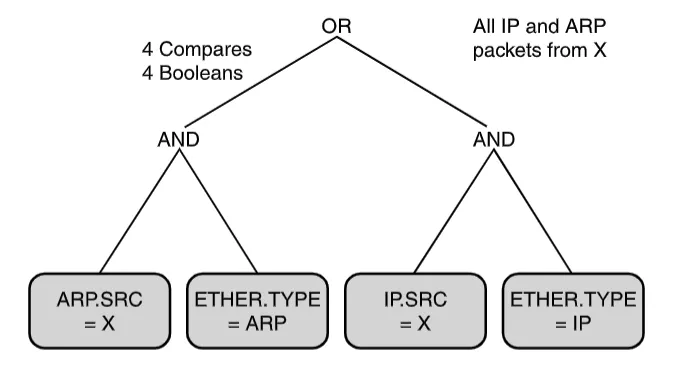
\includegraphics[width=0.8\textwidth]{../assets/ch04/ch04-4_3_包过滤-001.png}
\end{figure}
图8.1 传统的分层解复用是每一层利用层头部中的一个字段，将数据包解复用到上面的下一层软件。
传统上，解复用是通过使用接收到的消息各层头部中包含的解复用字段，逐层进行的。这种方式被称为
分层解复用，如图8.1所示。例如，在图中从下往上看，一个数据包可能通过以太网到达工作站。以太网
驱动程序会检查这个数据包，它会查看一个所谓的协议类型字段，以确定正在使用哪种路由协议（如
IP、IPX）。假设类型字段指定为IP，以太网驱动程序可能会向上调用IP软件。
在IP处理之后，IP软件会检查IP头部中的协议ID字段，以确定传输协议（如TCP或UDP？）。假设是
TCP，数据包将被传递给TCP软件。在完成TCP处理后，TCP软件会检查数据包中的端口号，以便将数
据包解复用到正确的客户端，例如，传递给实现HTTP的进程。
传统的解复用相当直接，因为每一层基本上都是对层头部中的某些字段进行精确匹配。这可以很容易地
实现，比如使用我们将在第10章描述的哈希方法。当然，每一层的查找成本会累积起来。
相比之下，本章重点讨论早期解复用，这在高速情况下是一项更具挑战性的任务。回顾图8.1，早期解复
用在数据包首次到达时，通过一次操作就能确定接收到的数据包所经过的整个协议路径。在最后一个例
子中，早期解复用可以一举确定网页数据包的路径是以太网、IP、TCP、网页。或许“分层解复用”是个
更好的术语。然而，本书采用了更被广泛接受的“早期解复用”这一名称。

                                                     1
一般来说，早期解复用的难点在于还需要允许应用程序灵活指定它们希望运行的底层协议，或者它们希
望接收其数据包的协议。这对于流量监测或安全应用特别有用。然而，如果早期解复用仅限于过去20年
已成为标准的TCP连接，那么问题就简单得多，并且（正如我们在第6章所示）可以通过数据包转向机制
来完成，该机制检查协议是否为TCP和IP（以太网中的类型字段），然后根据TCP四元组进行解复用。
回想一下，Linux通过两种方式之一进行“早期解复用”：要么使用TCP四元组的哈希值来分配负载（接收
数据包转向，即Receive Packet Steering或RPS），要么将数据包发送到运行应用程序的核心（接收流
转向，即Receive Flow Steering或RFS）。RFS也使用四元组的哈希值，但用它来索引一个表，表项指
向数据包应被转向的核心。
虽然这种基于简单哈希的机制在处理TCP和IP时效果很好，但它无法解决应用程序可以实时指定的其他协
议的早期解复用问题，例如流量监测应用所需的协议。这就是本章的主题。
本章的结构如下。8.1节阐述了早期解复用的原因，8.2节概述了高效解复用解决方案的目标。本章其余部
分研究了早期解复用的各种实现方式。本章从开创性的CMU/斯坦福数据包过滤器（CSPF）开始（8.3
节），接着介绍常用的伯克利数据包过滤器（BPF）（8.4节），最后介绍一些较新的方案，如
Pathfinder（8.5节）和DPF（8.6节）。
本章描述的解复用技术（以及所使用的相应原理）总结在表8.1中。
快速参考指南
伯克利数据包过滤器（BPF）是免费提供的。然而，其他解复用算法效率更高。希望设计解复用例程的
开发者应该考虑8.5节中描述的PathFinder。虽然动态数据包过滤器（DPF，见8.6节）速度更快，但许多
开发者可能会发现DPF中动态代码生成的需求是一个障碍。还要记得，对于TCP连接的早期解复用现在
已经成为标准，并且在Linux中可以通过各种转向机制实现。因此，本章中的技术仅对流量监测等灵活解
复用有用。
8.1 早期解复用的机遇与挑战
为什么早期解复用是个好主意呢？第6章讨论了以下基本动机。
 ● 灵活的用户级实现：早期解复用最初的原因是为了允许在用户级灵活实现协议，同时避免过多的上
   下文切换。
 ● 高效的用户级实现：随着时间的推移，开发者意识到早期解复用还可以通过最小化上下文切换次数
   来实现高效的用户级实现。主要的额外技巧是将协议实现构建为一个共享库，可以链接到应用程
   序。
请注意，随着针对TCP数据包的接收数据包转向原语的出现，如今在用户级实现TCP已经很容易。然
而，早期解复用还有其他优点。
 ● 数据包优先级排序：早期解复用允许对重要数据包进行优先级排序，并快速丢弃不必要的数据包。


                                                         2
   例如，第6章表明，通过对接收的数据包进行早期解复用，将数据包直接放入每个套接字队列中，可
   以缓解接收器活锁问题。这使得系统在过载时可以丢弃慢速进程的消息，同时允许表现良好的进程
   继续接收消息。更普遍地说，早期解复用对于通过服务区分来为流量流提供服务质量保证至关重
   要。如果所有流量都被解复用到一个公共的内核队列中，那么在过载期间共享缓冲区填满时，重要
   数据包可能会丢失。如今的路由器出于类似原因进行数据包分类（第12章和第14章）。早期解复用
   允许对数据流的处理进行显式调度；调度和计费可以结合起来，以防止诸如优先级反转等异常情
   况。
 ● 路径定制：一旦知道了数据包的路径，就可以对代码进行定制以处理该数据包，因为更广泛的上下
   文是已知的。例如，与其让每一层协议都检查数据包长度，不如本着P1原则只检查一次，避免明显
   的浪费。莫斯伯格（Mosberger）和彼得森（Peterson）在1996年将路径的理念发挥到了逻辑极
   致，他们描述了一种操作系统，其中路径是一等公民对象。
 ● 快速分发：本章和第6章已经通过数据包过滤器和用户级协议实现描述了这个想法的一个实例。早期
   解复用避免了每层的复用成本；更重要的是，它避免了有时在分层复用中可能产生的控制开销。
8.2 目标
如果早期解复用是个好主意，那么它容易实现吗？如果每个数据包在最外层（如数据链路层或网络层）
头部携带一些信息，用于标识最终端点，那么早期解复用就特别容易实现。这是P14原则的一个例子，即
在层头部传递信息。例如，如果网络协议是像ATM这样的虚电路协议，ATM虚电路标识符（VCI）可以
直接标识数据包的最终接收者。
然而，像IP这样的协议并没有提供这样的便利。多协议标签交换（MPLS）确实提供了这种便利，但正如
第11章所描述的，MPLS通常仅在路由器之间使用。即使使用像ATM这样的协议，可用的VCI数量也可能
有限。由于没有单个解复用字段，因此需要更复杂的数据结构，我们称之为数据包过滤器或数据包分类
器。当然，正如我们一开始所指出的，仅针对TCP连接使用TCP四元组的哈希值来实现这一点很容易，
但更通用的解决方案需要更好的数据结构。
这样的数据结构将完整的数据包头部作为输入，并将输入映射到一个端点或路径。直观地说，数据包的
端点代表接收应用程序进程，而路径代表在端点消耗数据包之前处理数据包时需要调用的协议序列。在
描述如何构建数据包过滤器之前，以下是一个好的早期解复用算法的目标。
 ● 安全性：许多早期解复用算法是在内核中基于用户级程序的输入实现的。每个用户程序P指定它希望
   接收的数据包。与Java程序一样，设计者必须确保不正确或恶意的用户不会影响其他用户。即使在
   今天，这对于流量监测也尤为重要。
 ● 速度：由于解复用是实时进行的，早期解复用代码应该快速运行，特别是在只指定了单个过滤器的
   情况下。
 ● 可组合性：如果N个用户程序指定了描述它们期望接收的数据包的数据包过滤器，理想情况下，实现
   应该将这N个单独的数据包过滤器组合成一个复合数据包过滤器。复合过滤器应该具有这样的特性：
                                                      3
  搜索复合过滤器比单独搜索N个过滤器中的每一个都要快，特别是对于较大的N。
本章从一个温和的生物学视角出发，描述了一系列数据包过滤器种类，每一种后续的改进都比前一种更
能实现这些目标。不出所料，最早的种类几乎已经“灭绝”，尽管它因其简单性和历史意义而值得关注。
8.3 CMU/斯坦福数据包过滤器：开创性的数据包过滤器
CMU/CSPF（莫古尔等人，1987年）是为了在Mach操作系统中实现用户级协议而开发的。在CSPF模型
中，应用程序向内核提供一个程序，描述它们希望接收的数据包。应用程序A提供的程序对数据包头部进
行操作，如果数据包应该被路由到应用程序A，则返回true。就像老款德州仪器计算器一样，这种编程语
言是一种基于栈的表达式树模型实现。




如\begin{figure}[htbp]
\centering
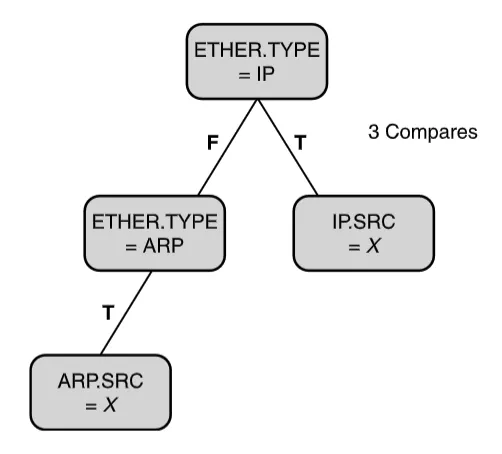
\includegraphics[width=0.8\textwidth]{../assets/ch04/ch04-4_3_包过滤-002.png}
\end{figure}
图8.2所示，树的叶子代表对数据包头部的简单测试谓词。一个测试谓词的例子是与固定值的相等比
较；例如，在图8.2中，ETHER.TYPE = ARP表示检查接收到的数据包中的以太网类型字段是否与为ARP
（地址解析协议）数据包指定的常量值匹配。树中的其他节点代表布尔运算，如AND和OR。
因此，图8.2中表达式树的左子树代表从源IP地址X发送的任何ARP数据包，而右子树代表从源IP地址X发
送的任何IP数据包。由于根节点代表一个OR操作，整个树表示请求由源X发送的所有IP或ARP数据包。这
样的表达式可以由调试工具代表希望检查来自源X的IP流量的用户提供给内核。

 图片加载失败
虽然表达式树模型提供了一种过滤器的声明性模型，但实际上这些过滤器使用一种命令式的基于栈的语
言来描述表达式树。为了确保安全性，CSPF提供了功能有限的栈指令；为了限制运行时间，它没有跳转
或循环结构。安全性还通过实时检查程序的加载和存储来实现，以消除非法的内存引用。因此，会监控
栈引用以确保其在栈范围内，并且会检查对数据包的引用以确保其在正在解复用的数据包长度范围内。
8.4 伯克利数据包过滤器：实现高性能监测

                                                      4
CSPF通过使用功能有限的指令和对内存访问进行运行时边界检查来保证安全性。然而，CSPF不具备可
组合性，并且在速度方面存在问题。数据包过滤器设计的下一个变革是引入了BPF（麦卡恩和雅各布
森，1993年）。
BPF的设计者特别希望将BPF用作高性能网络监测工具（如tcpdump）的基础，对于这些工具来说，速度
至关重要。他们注意到，即使使用如图8.2所示的单个CSPF表达式树，也存在两个速度问题。
 ● 架构不匹配：CSPF栈模型是为PDP - 11设计的，因此与现代RISC架构不太匹配。首先，必须模拟
   栈，这意味着每次进行布尔运算时都需要额外的内存引用来更新栈指针。其次，RISC架构通过将变
   量存储在快速寄存器中并直接从寄存器进行计算来提高效率。因此，为了在RISC架构中提高效率，
   尽可能多的计算应该在寄存器值被重用之前使用该寄存器值进行。例如，在图8.2中，CSPF模型每
   次引用以太网类型字段（检查与ARP和IP的相等性）时都将导致两次单独的内存加载。在现代机器
   上，更好的方法是将类型字段存储在寄存器中，并一次性完成所有与类型字段的比较，以减少内存
   引用。
 ● 模型效率低下：即使忽略CSPF所需的额外内存引用，表达式树模型通常也会导致比严格必要的操作
   更多。例如，在图8.2中，注意到CSPF表达式需要进行四次比较才能评估所有叶子节点。然而，注
   意到一旦我们知道以太网类型等于ARP（如果我们从左到右评估），那么额外检查IP源地址是否等于
   X就是多余的（原则P1，避免浪费）。主要问题是在表达式树模型中，随着计算的进行，没有办
   法“记住”数据包解析状态。这可以通过构建状态机的新模型来解决。
CSPF还有另外两个小问题。它只能解析数据包头部中固定偏移量处的字段；因此，它不能用于访问封装
在IP头部内的TCP头部，因为这需要首先解析IP头部长度字段。CSPF还仅使用16位字段处理头部，这使
得处理32位字段（如IP地址）所需的操作数量增加了一倍。
BPF通过以下方式解决了这些问题。首先，它用基于寄存器的语言取代了基于栈的语言，并带有一个间
接操作符，可以帮助解析TCP头部。使用“LOAD [12]”这样的命令将指定数据包偏移量处的字段加载到寄
存器中，该命令加载以太网类型字段，以太网类型字段恰好从以太网数据包的起始位置偏移12字节处开
始。
BPF然后可以进行比较和跳转，如“JUMP_IF_EQUAL ETHERTYPE_IP, TARGET1, TARGET2”。这条指
令将累加器寄存器与IP以太网类型字段进行比较；如果比较结果为真，程序跳转到行号TARGET1；否
则，跳转到TARGET2。BPF允许以8位、16位和32位块进行操作。




                                                                 5
更根本的是，BPF使用计算的控制流图（CFG）模型，如\begin{figure}[htbp]
\centering
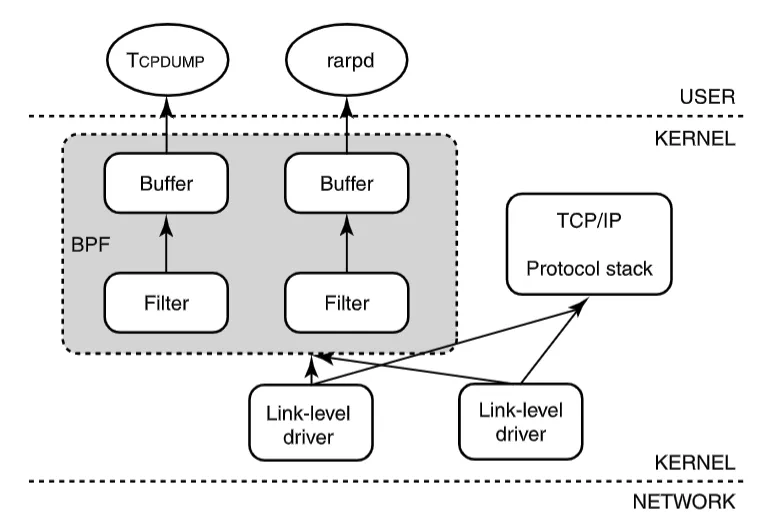
\includegraphics[width=0.8\textwidth]{../assets/ch04/ch04-4_3_包过滤-003.png}
\end{figure}
图8.3所示。这基本上是一个从根节点开始的状
态机，其状态在每个节点处更新，然后转移到其他节点状态，转移用指向其他节点的弧线表示。状态机
首先检查以太网类型字段是否为IP；如果是，则只需检查IP源字段是否为X即可返回true。如果不是，则
需要检查以太网类型字段是否为ARP以及ARP源是否为X。注意，在状态机的左分支中，我们不检查IP源
地址是否为X。因此，图8.3中最坏情况下的比较次数为3次，而图8.2中为4次。
BPF被用作许多工具的基础，包括著名的tcpdump工具，用户可以使用该工具获取链路上流动的TCP数
据包的可读记录。BPF被嵌入到BSD内核中，如\begin{figure}[htbp]
\centering
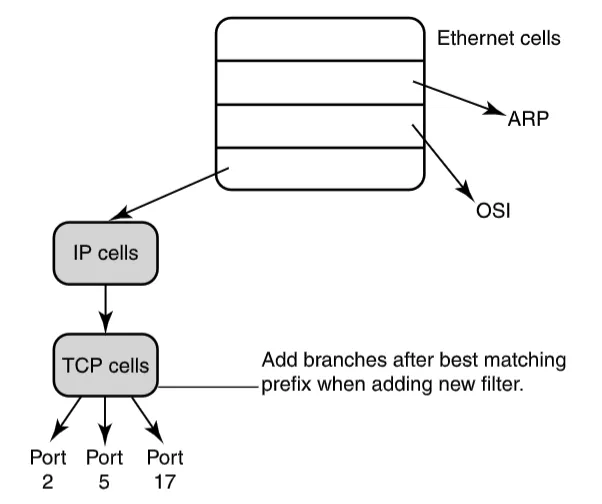
\includegraphics[width=0.8\textwidth]{../assets/ch04/ch04-4_3_包过滤-004.png}
\end{figure}
图8.4所示。




当数据包到达网络链路（如以太网）时，数据包由适当的链路层驱动程序处理，通常会传递到TCP/IP协
议栈进行处理。然而，如果BPF处于活动状态，则首先调用BPF。BPF根据当前指定的每个用户过滤器检
查数据包。对于每个匹配的过滤器，BPF将过滤器指定的尽可能多的字节复制到每个过滤器的缓冲区

                                                 6
中。注意，多个BPF应用程序可能会导致同一数据包的多个副本被缓冲。该图还显示了除tcpdump之外
的另一个常见BPF应用程序，反向ARP守护进程（rarpd）。
BPF还有两个对高性能也很重要的小特性。首先，BPF在缓冲之前过滤数据包，这避免了不必要的浪费
（P1），因为大多数接收到的数据包可能不是BPF应用程序想要的。这种浪费不仅包括缓冲区的内存，
还包括复制所需的时间（第5章）。
其次，由于数据包可能到达得非常快，而read()系统调用相当慢，BPF允许批处理（P2c），并允许在一
次调用中将多个数据包返回给监测应用程序。为了处理这个问题并区分数据包边界，BPF为每个数据包
添加一个头部，其中包括时间戳和长度。tcpdump的用户不必使用这个接口；相反，tcpdump提供了一
个更用户友好的接口：接口命令被编译为BPF指令。

 图片加载失败

8.5 Pathfinder：分解常见检查
BPF相较于CSPF是一种更优化的方案，因为它提高了单个过滤器的处理速度。然而，每个数据包仍必须
依次与每个过滤器进行比较。因此，处理时间会随着过滤器数量的增加而延长。幸运的是，对于典型的
BPF使用场景而言，这并非问题。例如，一个典型的tcpdump应用程序可能仅向BPF提供少量过滤器。
然而，在早期解复用用于区分大量数据包流或路径的情况下，情况就有所不同了。特别是，每个TCP连
接可能会提供一个过滤器，而繁忙服务器中的并发TCP连接数量可能非常大。为了应对这种环境变化
（用户级网络），出现了另一种成功的改进方案——Pathfinder（Bailey等人，1994年）。Pathfinder超
越了BPF，它具备可组合性，这使得它能够扩展以服务大量用户。
为了理解Pathfinder的解决方案，假设有500个过滤器，每个过滤器除了指定不同的TCP端口对外，其他
内容完全相同（以太网类型字段为IP，IP协议类型为TCP ）。如果依次处理每个过滤器，就需要将数据
包的以太网类型与（相同的）IP以太网类型字段进行500次比较，并将IP协议字段与（相同的）TCP协议
值进行500次比较。这显然是一种浪费（原则P1）。
接下来，将数据包中的TCP端口号与500个过滤器中每个指定的500个端口对进行比较，这种做法的弊端
并不明显。然而，这与线性搜索精确匹配的原理完全相同。这表明，当单个过滤器数量较多时，将所有
单个过滤器集成到一个复合过滤器中，可以显著减少不必要的比较。具体而言，可以使用哈希（原则
P15，使用高效的数据结构）来进行精确搜索，这样就可以用少量比较替代500次比较。
正如我们在本章开头反复提到的，如果仅处理TCP连接，这种哈希的概念已经通过接收数据包转向机制
实现。但如果想要对通用协议进行灵活的解复用，则需要更复杂的数据结构。
用于此目的的数据结构如图8.5所示。其基本思想是将BPF中每个过滤器的控制流图（CFG）进行叠加，
以便对同一字段的所有比较都放置在单个节点中。最后，每个节点都被实现为一个哈希表，其中包含所

                                                            7
有比较值，从而用哈希查找替代线性搜索。




 图片加载失败
图8.5展示了一个示例，其中至少有四个过滤器，其中两个指定目的端口号为2和5的TCP数据包；目前，
忽略指向TCP端口17的虚线，稍后将其作为过滤器插入的示例。除了TCP过滤器外，还有一个或多个指
定ARP数据包的过滤器，以及一个或多个指定使用OSI协议数据包的过滤器。
根节点对应以太网类型字段；哈希表包含过滤器中使用的每个可能的以太网类型字段值。每个节点条目
都有一个值和一个指针。因此，ARP条目指向进一步指定必须接收的ARP数据包类型的节点；OSI条目也
是如此。最后，对应IP的以太网类型字段指向对应IP协议字段的节点。
在IP协议字段节点中，对应TCP（值为6）的一个值将指向TCP节点。在TCP节点中，有三个值分别指向
目的端口值为2和5的过滤器（请记住，17尚未插入）。当一个TCP数据包到达时，解复用过程如下。
从根节点开始搜索，对以太网类型字段进行哈希处理，以找到与IP对应的匹配值。该值的指针将指向IP节
点，在IP节点中，对IP协议类型字段进行哈希处理，以找到与TCP对应的匹配值。该值的指针将指向TCP
节点，在TCP节点中，对数据包中的目的端口值进行哈希处理，以找到最终匹配的过滤器。
Pathfinder的数据结构与一种常见的数据结构——前缀树（trie）非常相似，第11章将更全面地介绍前缀
树。简而言之，前缀树是一种树结构，其中每个节点包含一个指向子树的指针数组；每个数组为固定字
符集中的每个可能值包含一个指针。
为了在前缀树中搜索关键字，需要将关键字分解为字符，并使用第i个字符对从根节点开始路径上的第i个
节点进行索引。以这种方式在节点i进行搜索会得到一个指针，该指针指向节点i + 1，然后在节点i + 1中
继续递归搜索。可以将Pathfinder结构视为对前缀树的扩展，它使用数据包头部字段（例如以太网类型字
段）作为连续的搜索字符，并使用哈希表替代每个节点中的数组。

                                                     8
众所周知，前缀树能够快速插入新的关键字。基于这种相似性，Pathfinder拥有快速插入或删除过滤器的
算法也就不足为奇了。例如，考虑插入一个对应TCP端口17的新过滤器。与前缀树一样，插入算法首先
搜索这个新过滤器的最长匹配前缀（第11章）。
这个最长匹配对应于路径“以太网类型 = IP，IP协议 = TCP”。由于此路径已由其他两个TCP过滤器创
建，因此无需重复创建。插入算法只需添加与新过滤器中超出最长匹配部分对应的分支（在这种情况下
是单个分支）。因此，只需更新TCP节点中的哈希表，添加一个指向端口17过滤器的新指针即可。
更准确地说，Pathfinder中的基本原子单元称为单元格（cell）。一个单元格指定数据包头部中的一个位
字段（使用偏移量、长度和掩码）、一个比较值和一个指针。例如，忽略指针，检查IP头部中协议字段
的单元格为(9, 1, 0xff, 6)——该单元格指定应将IP头部的第十个字节用全1掩码进行掩码处理，并与值6进
行比较，值6代表TCP。
给定用户的单元格串联在一起形成该用户的模式。多个模式通过不重新创建已存在的单元格进行叠加，
从而形成Pathfinder前缀树。最后，指定相同位字段但不同值的多个单元格使用哈希表进行合并。
除了使用哈希表替代数组外，Pathfinder还超越了前缀树，它使每个节点都包含任意代码。实际上，
Pathfinder认识到前缀树是一种特殊的状态机，可以通过在前缀树的每个节点执行任意操作来进行扩展。
例如，Pathfinder可以通过允许除前面描述的比较单元外的可加载单元来处理分片数据包。这是必要的，
因为对于分片数据包，只有第一个分片指定TCP头部；将各个分片链接在一起的是第一个分片中描述的
公共数据包ID。
Pathfinder通过在第一个分片到达后放置一个额外的可加载单元格（以及指定源地址等的正常IP比较单元
格）来处理分片，该可加载单元格加载数据包ID。通过不指定单元格中的比较值来指定一个单元格为可
加载单元格。
可加载单元格最初不是Pathfinder前缀树的一部分，而是IP单元格的一个属性。如果第一个分片匹配，则
将加载的单元格插入到Pathfinder前缀树中，现在它可以根据新加载的数据包ID匹配后续分片。在所有分
片都处理完毕后，可以删除这个新添加的单元格。最后，Pathfinder通过将后续分片的处理推迟到第一个
分片到达，来处理后续分片先于第一个分片到达的情况。
8.6 动态数据包过滤器：编译器来帮忙
到目前为止，Pathfinder被描述为一种树形结构，但实际上其数据结构可以泛化为有向无环图
（DAG）。有向无环图允许两个不同的过滤器在Pathfinder图中最初沿着不同的路径，然后汇聚到共享
的路径后缀。例如，在为目的端口80的TCP数据包提供过滤器时，该数据包可能是分片的，也可能是非
分片的，这种情况下有向无环图就很有用。虽然需要为分片和非分片的IP数据包分别指定不同的单元格
路径，但这两条路径可以指向同一组TCP单元格。
最后，Pathfinder还允许使用从单元格引出的“或”（OR）链接。其原理是，每个“或”链接指定一个值，
检查每个“或”链接以找到匹配的值，然后沿着该链接继续处理。

                                                        9
为了在拥塞期间对数据包进行优先级排序（如第6章所述），解复用例程必须在接收数据包所需的最短时
间内完成。Pathfinder的软件实现速度很快，但通常无法跟上线路速率。幸运的是，Pathfinder状态机可
以在硬件中实现，从而以线路速率运行。这与使用前缀树进行IP查找以线路速率工作的方式类似（第11
章）。
Bailey等人（1994年）描述的硬件原型为了提高速度牺牲了部分功能。它以16位块为单位工作，仅实现
了最基本的单元格功能；不过，它在硬件中实现了分片处理。功能的限制意味着Pathfinder硬件只能用作
缓存，以加速处理不太常见情况的Pathfinder软件。一个运行频率为100MHz的原型设计预计处理一个40
字节的TCP消息需要200纳秒，这对于1.5Gbps的速率来说已经足够。通过使用更快的时钟频率、更快的
内存和流水线遍历状态机，该设计可以扩展到更高的线路速率。
动态数据包过滤器：编译器来帮忙
Pathfinder的故事以借助硬件实现高速解复用作为结尾。鉴于如今大多数工作站和个人电脑不太可能配备
专用的解复用硬件，实现者似乎必须在早期解复用带来的灵活性和软件分类器有限的性能之间做出选
择。因此，高性能TCP（Clark等人，1989年）、主动消息（von Eicken等人，1992b）和远程过程调用
（RPC）（Thekkath等人，1993年）的实现都采用手工编写的解复用例程，也就不足为奇了。
动态数据包过滤器（DPF）（Engler和Kaashoek，1996年）试图同时兼顾灵活性和性能。DPF基于
Pathfinder前缀树的理念，但它通过在每次添加或删除过滤器时将分类器重编译为机器代码，消除了单元
格处理中固有的间接操作和额外检查。实际上，DPF为前缀树中的每个单元格生成单独的优化代码，而
不是使用可以解析前缀树中任意单元格的通用未优化代码。
DPF基于动态代码生成技术（Engler，1996年），该技术允许在运行时生成代码，而不是在内核编译时
生成。DPF应用了原则P2，即时间上的计算转移。需要注意的是，这里的运行时指的是分类器更新时
间，而不是数据包处理时间。
这一点很关键，因为这意味着DPF必须能够以足够快的速度重新编译代码，以免减慢分类器的更新速
度。例如，建立一个连接可能需要几毫秒，同时需要添加一个过滤器来识别端点。相比之下，以千兆速
率接收一个最小尺寸的数据包可能只需要几微秒。尽管有这样的时间差，但实现亚毫秒级的编译时间仍
然具有挑战性。
为了理解为何为每个单元格使用专门的代码是有用的，需要了解Pathfinder中单元格处理效率低下的两个
常见原因：
 ● 解释开销：Pathfinder代码在内核代码编译时确实会被编译为机器指令。然而，从某种意义上说，这
    些代码是在“解释”一个通用的Pathfinder单元格。例如，考虑一个指定了四元组（偏移量、长度、
    掩码、值）的通用Pathfinder单元格C。当数据包P到达时，用于检查单元格是否与数据包匹配的理
    想化机器代码如下：


                                                        10
 1                        将单元格中指定的偏移量加载到寄存器R1中 *)
     LOAD R1, C(Offset); (*
 2                        将单元格中指定的长度加载到寄存器R2中 *)
     LOAD R2, C(length); (*
 3                        将偏移量指定的数据包字段加载到R3中 *)
     LOAD R3, P(R1, R2); (*
 4                      将单元格中指定的掩码加载到寄存器R1中 *)
     LOAD R1, C(mask); (*
 5   AND R3, R1; (* 按照单元格中的指定对数据包字段进行掩码处理 *)
 6                       将单元格中指定的值加载到寄存器R2中 *)
     LOAD R2, C(value); (*
 7   BNE R2, R3; (* 如果掩码处理后的数据包字段不等于值，则进行分支 *)
请注意，第1、2、4和6行中的额外指令和额外内存引用是为了从通用单元格加载参数，以便后续进行比
较。
 ● 安全检查开销：由于用户编写的数据包过滤器不可信，所有实现都必须进行检查以防范错误。例
   如，必须在运行时检查对数据包字段的每次引用，以确保其在当前正在解复用的数据包范围内。同
   样，需要实时检查内存引用的对齐情况；在许多机器上，未对齐到字大小倍数的内存引用可能会导
   致陷阱。在进行这些额外检查后，前面显示的代码片段会变得更加复杂，并且包含更多指令。
通过为每个单元格专门编写代码，DPF可以利用将单元格添加到Pathfinder图时已知的信息，消除这两个
开销来源。
 ● 消除解释开销：由于DPF在创建单元格时就知道所有单元格参数，因此它可以生成将单元格参数直
   接编码为机器代码立即操作数的代码。例如，前面解析通用Pathfinder单元格的代码片段可以简化为
   更紧凑的特定单元格代码：
 1                             将数据包字段加载到R3中 *)
     LOAD R3, P(offset, length); (*
 2   AND R3, mask; (* 使用指令中的掩码对数据包字段进行掩码处理 *)
 3   BNE R3, value; (* 如果字段不等于值，则进行分支 *)
请注意，加载参数的额外指令以及（更重要的）额外内存引用已经消失，因为参数直接作为立即操作数
放置在指令中。
 ● 降低安全检查开销：在预期情况下（原则P11），可以通过在编译时推断大多数引用是字对齐的来减
   少对齐检查。这可以通过检查完整的过滤器来实现。如果初始引用是字对齐的，并且当前引用（偏
   移量加上所有先前头部的长度）是字长度的倍数，那么该引用就是字对齐的。只有在编译时推断失
   败时（例如，在进行间接加载时，如可变大小的IP头部），才需要进行实时对齐检查。同样，在编
   译时可以确定任何单元格中使用的最大偏移量，并在数据包处理之前进行一次检查，以确保最大偏
   移量在当前数据包的长度范围内。
一旦发现了好的方法，就应该充分利用它。DPF进一步利用编译时的知识进行如下优化。第一个优化是
将对相邻字段的小访问合并为一次大访问。其他优化将在练习中探讨。
DPF存在以下潜在缺点，但通过精心设计可以加以控制：
 ● 重新编译时间：回想一下，当向Pathfinder前缀树添加过滤器时（图8.5），只需创建原始前缀树中



                                                    11
   不存在的单元格。DPF通过缓存现有单元格的代码，并将这些代码直接复制（而不是从头重新创
   建）到新的分类器代码块中，对这种预期情况进行了优化（原则P11）。只有新创建的单元格才需要
   生成新代码。同样，当向哈希表添加新值时（例如，图8.5中添加的新TCP端口），除非哈希函数发
   生变化，否则代码将被重用，只需更新哈希表。
 ● 代码膨胀：解释的一个标准优点是代码更紧凑。为每个单元格生成专门的代码似乎会产生过多的代
   码，尤其是在过滤器数量较多的情况下。庞大的代码占用空间可能会反过来导致指令缓存性能下
   降。然而，仔细研究发现，DPF生成的不同代码块数量仅与所有过滤器检查的不同头部字段数量成
   比例。这比过滤器的数量更具扩展性。例如，对于10000个同时存在的TCP连接，DPF可能只生成三
   个专门的代码块：一个用于以太网头部，一个用于IP头部，以及一个用于TCP头部的哈希表。
DPF的最终性能数据令人印象深刻。在可比平台上，DPF解复用消息的速度比Pathfinder快13 - 26倍
（Engler和Kaashoek，1996年）。不过，添加过滤器的时间仅比Pathfinder慢三倍。动态代码生成只占
这种插入开销增加的40%。
无论如何，较大的插入成本似乎是为更快的解复用付出的合理代价。最后，DPF解复用例程似乎可以与
手工编写的解复用例程相媲美甚至超越它们；例如，一个用于解复用IP数据包的DPF例程只需要18条指
令，而Clark（1985年）报告的早期值为57条指令。虽然这两个实现是在不同的机器上进行的，但这些数
字在一定程度上体现了DPF的性能优势。
DPF带来的启示有两点。第一，DPF表明可以同时实现性能和灵活性。就像编译器生成的代码通常比手工
编写的代码更快一样，DPF代码似乎使手工编写解复用代码不再必要。第二，DPF表明以线路速率进行解
复用可能不需要硬件支持。实际上，在硬件实现中允许在创建过滤器时进行动态代码生成可能很困难。
软件解复用可以使用更便宜的工作站；它还可以使解复用代码从处理器速度的提升中受益。
技术变革可能使设计假设失效
在架构和操作系统领域，有不少创新在最初使用后被弃用，之后又重新被采用。这可能看起来像是时尚
的反复（比如“1995年褶边衣领又流行起来”），或者是重新发明轮子（即“天下并无新事” ），但要知道
何时以新的形式重拾旧想法，需要对当前技术有深入理解。
以电话网络核心为例，过去它通过模拟信号传输语音通话。随着光纤和晶体管的出现，如今电话网络核
心的大部分语音信号都采用T1和SONET层级体系进行数字传输。然而，随着光纤波分复用技术的出现，
至少有一些人讨论回归模拟传输。
因此，优秀的系统设计师必须持续关注现有技术，查看系统设计假设是否已不再成立。莫古尔等人在
1987年提出CSPF时提到了动态编译的概念，但并未深入探讨。CSPF的设计者认为，针对特定的过滤器
集定制代码（每次添加过滤器时都重新编译分类器代码）过于“复杂”。
在CSPF设计之时，动态编译可能速度较慢，而且无法在不同系统间移植；由于存在其他瓶颈，当时采用
动态编译所带来的收益也很有限。然而，到了设计DPF的时候，包括VCODE（恩格勒，1996年）在内的

                                                         12
许多系统已经设计出了相当快速且可移植的动态编译基础设施。DPF的其他分类器实现方式也消除了其
他瓶颈，这使得动态编译的优势更加明显。
8.7 结论
虽说“需求是发明之母”这句话略显陈词滥调，但它往往是正确的。新的需求推动新的创新；而没有需求
则解释了为什么创新没有更早出现。CSPF过滤器是在主要需求为避免进程上下文切换时实现的；在实现
这一目标后，提高过滤器性能就只是次要影响了。BPF是在主要需求为高效实现少数过滤器，以使像
tcpdump这样的监测工具能以接近线路速率运行时实现的。在实现这一目标后，扩展到大量过滤器的需
求似乎就没那么重要了。
Pathfinder是为了支持x - kernel（Hutchinson和Peterson，1991）中的用户级网络，并允许Scout
（Mosberger和Peterson，1996）将路径作为一等对象进行多方面利用而实现的。在找到了可行的硬件
实现方案后，或许提升软件性能就显得不那么重要了。DPF是为了在可扩展操作系统的环境中（Engler等
人，1995），实现高性能网络以及完全的应用级灵活性而设计的。表8.1总结了本章所使用的技术以及相
关的主要原理。
然而，鉴于如今TCP/IP的广泛应用，以及主流操作系统中数据包转向机制的可用性，目前还不清楚
Pathfinder和DPF在今天是否值得采用，毕竟它们增加了复杂性。BPF对于监测工具而言仍然有用。




                                                                 13


\chapter{现代优化技术}
% 来源: 19c9fbb8-d222-8ee0-8000-000075e33130_4.4_现代优化技术.pdf
% 提取时间: 2026-02-28T22:51:36+08:00

4.4 现代优化技术
Linux内核及网络技术领域又涌现出一系列更高级的优化手段。这些技术进一步突破了传统网络栈的瓶
颈，特别是在处理超高速网络（如100Gbps+）和超低延迟场景下表现卓越。以下是主要的优化方向及代
表性技术：
1.   XDP（eXpress Data Path）
XDP是Linux内核4.8+引入的超高性能网络数据路径，直接在网卡驱动层处理数据包：
 ● 原理：

    ○ 使用eBPF（Extended Berkeley Packet Filter）程序在网卡接收数据包后立即执行，允
      许快速决策（转发、丢弃、修改）。
    ○ 完全在内核态处理，甚至可在解析IP头前就完成过滤，避免不必要的协议栈处理。
 ● 优势：
    ○ 亚微秒级延迟，吞吐量比NAPI高3-5倍。
    ○ 动态可编程：可实时加载/更新eBPF程序，无需重启内核。
 ● 应用：高性能防火墙、DDoS防护、流量分流等。


2.   硬件卸载（Hardware Offload）
将部分网络处理任务交给网卡硬件完成，减轻CPU负担：
TCP/UDP分段卸载（TSO/GSO）
 ● 原理：网卡硬件自动将大尺寸数据包分割为符合MTU的小数据包，减少CPU的分段开销。

校验和计算卸载
 ● 原理：网卡硬件计算TCP/UDP/IP校验和，避免CPU处理。

SR-IOV（Single Root I/O Virtualization）
 ● 原理：网卡虚拟化出多个虚拟功能（VF），每个VF可直接分配给虚拟机或容器，实现近乎物
      理网卡的性能。
3.   内核旁路（Kernel Bypass）技术
传统网络数据包需经过内核协议栈处理，存在上下文切换和内存复制开销。内核旁路技术绕过内
核，让应用程序直接访问网卡硬件，大幅降低延迟：

                                                                 1
DPDK（Data Plane Development Kit）
 ● 原理：通过UIO（Userspace I/O）或VFIO（Virtual Function I/O）机制，允许用户空间程序
       直接操作网卡队列，绕过内核协议栈。
     ● 优势：减少内核上下文切换和内存拷贝，实现微秒级延迟；支持多线程并行处理数据包。

     ● 应用：网络功能虚拟化（NFV）、高性能防火墙、负载均衡器等。

PF_RING
 ● 原理：在内核中优化网络数据包的接收路径，提供零拷贝机制，同时允许用户空间程序快速访
       问数据包。
     ● 优势：相比DPDK，对内核依赖更强，但实现更轻量，适合特定场景（如流量监控）。


4.   零拷贝（Zero-Copy）技术
减少数据包在内存中的复制次数是提升性能的关键：
内核内零拷贝
 ● 示例：Linux的 
             splice()、 
                        sendfile()系统调用，在内核空间直接完成文件或socket
         间的数据传输，避免用户空间与内核空间的来回拷贝。
用户空间零拷贝
     ● DPDK通过内存映射（mmap）让用户空间程序直接访问网卡缓冲区，无需内核复制。
     ● RDMA与内存语义网络：基于RDMA技术实现远程内存直接访问，消除传统网络栈的开销。


5.   数据面和控制面分离

5.1  软件定义网络（SDN）与控制面/数据面分离架构
软件定义网络（SDN）是一种革命性的网络架构范式，其核心思想是将网络的控制平面与数据平面解耦，
实现网络流量的集中化、可编程控制。

传统网络设备（如路由器、交换机）将控制逻辑（如路由协议、策略决策）与数据转发功能紧密集成
在硬件中，这种紧耦合架构导致网络灵活性受限、配置复杂、创新缓慢。SDN通过以下方式改变了这一
现状：
● 控制平面集中化：将原本分散在各设备中的控制逻辑集中到SDN控制器（Controller）上，控制器
  维护全局网络拓扑视图，通过南向接口（如OpenFlow）向数据平面设备下发流表规则。
● 数据平面简化：数据平面设备（OpenFlow交换机）专注于高速数据包转发，无需运行复杂的路由
  协议，其转发行为完全由控制器通过流表决定。
● 网络可编程性：网络管理员可通过北向API（REST API、Python SDK等）编写应用程序，动态定义
  网络行为，实现流量的灵活调度、负载均衡、安全策略部署等。

典型应用场景：
● 数据中心网络虚拟化：SDN可自动为不同租户创建隔离的虚拟网络，支持网络功能虚拟化（NFV）
  和微服务架构。
● 流量工程与QoS保障：基于全局流量视图，SDN控制器可动态计算最优路径，避开拥塞链路，保障
  关键业务的服务质量。
● 网络安全与微分段：通过细粒度的流表控制，实现东西向流量的微分段隔离，有效遏制横向攻击
  蔓延。

OpenFlow协议是SDN南向接口的事实标准，它定义了控制器与交换机之间的通信协议，允许控制器
下发、修改、删除流表项。然而，传统OpenFlow主要支持固定功能的匹配字段（如MAC地址、IP地址、
端口号），对更复杂的数据包处理（如深度包检测、自定义协议解析）支持有限，这催生了可编程数据
平面技术的发展。


6.  AI时代的网络架构演进

随着人工智能（AI）特别是大语言模型（LLM）训练需求的爆发式增长，数据中心网络面临着前所未有的挑
战。传统面向通用云计算设计的网络架构，在处理AI训练特有的流量模式时暴露出诸多局限性。

6.1  传统Clos网络的局限性

Clos网络架构因其高带宽、无阻塞的特性，长期以来是数据中心网络的主流选择。该架构采用多级交换
机互联，如典型的三层结构：脊（Spine）-叶（Leaf）-接入（ToR）。然而，在AI训练场景下，这种架构面
临根本性挑战：

类比理解：传统Clos网络如同一座设计精良的城市道路系统，能够高效处理日常通勤的多样化交通流。但
当需要运输超大型的特殊货物（如火箭部件）时，即使道路再宽敞，单一的运输路线也可能成为瓶颈。

核心问题源于AI训练工作负载的三个关键特征：

● 大象流（Elephant Flows）：AI训练任务生成持续时间长、数据量巨大的单条数据流。在分布式训练
  中，梯度同步和参数更新可能涉及数百GB甚至TB级别的数据传输，这些"大象流"一旦哈希到某条
  特定链路，就会造成该链路的严重拥塞。
  
  定义：大象流（Elephant Flows）指持续时间较长、数据量巨大的网络数据流，与短暂的"老鼠流"
  （Mouse Flows）相对。在AI训练场景中，典型的All-Reduce集体通信会产生大量大象流。

● 低熵流量（Low Entropy）：AI训练中的集体通信（Collective Communication）如All-Reduce、
  All-to-All等操作，涉及固定数量的GPU节点之间的大规模数据交换。这导致流量模式高度规律、
  可预测，可用路径的多样性（熵）极低。
  
  定义：低熵流量（Low Entropy Traffic）指网络流量中具有高度规律性和可预测性的数据流集合，
  其随机性（熵）不足以充分发挥ECMP（等价多路径路由）的负载均衡效果。

● 次优的Fabric利用率：由于上述两个因素的叠加效应，Clos网络中各链路的带宽利用率呈现严重
  的偏斜分布。部分链路过载导致拥塞和队头阻塞（Head-of-Line Blocking），而大量链路则处于
  空闲状态，造成昂贵的网络投资无法充分发挥效用。

Meta公司在实践中尝试了多种解决方案来缓解这些问题，包括BGP策略优化、负载感知ECMP、基于流量
工程的预计算等，但每种方案都存在明显局限：

● BGP策略优化：通过固定上行链路来降低低熵问题，但无法处理链路故障后的回退场景。
● 负载感知ECMP：能够感知大象流并重新哈希，但参数调优复杂，且可能导致数据包乱序，这对
  依赖顺序传输的RDMA通信是灾难性的。
● 流量工程预计算：根据模型特征预配置Leaf交换机，但随着网络规模扩大，配置复杂度呈指数增长，
  且集中式方案对故障响应缓慢。

6.2  Meta的解决方案：DSF架构

面对传统架构的根本性局限，Meta开发了DSF（Disaggregated Scheduled Fabric，解耦调度型Fabric）
作为下一代AI训练网络架构。

定义：DSF（Disaggregated Scheduled Fabric）是Meta开发的面向AI训练的下一代网络架构，通过将
传统单体机箱式交换机解耦为分布式组件，结合信元交换和信用机制，实现近最优的负载均衡和拥塞
控制。

DSF的核心创新在于其"双域架构"，将网络划分为两个逻辑域：

● 以太网域（Ethernet Domain）：连接服务器端点，保持与传统网络设备的兼容性，处理标准的
  以太网帧。
  
● Fabric域（Fabric Domain）：在DSF内部，数据包被切分为等长的信元（Cells），通过信元喷射
  （Cell Spraying）技术均匀分布在所有可用路径上，在出口处重新组装为完整数据包后交付。

这种架构类似于现代物流系统：传统网络如同一个包裹从起点到终点只能走一条固定的路线，而DSF
则像是一个高度自动化的分拣中心，将每个包裹拆分为标准化的小件，通过多条并行的传送带同时运输，
在目的地重新组合。

DSF由两类核心组件构成：

● 接口节点（Interface Nodes, INs）/架顶解耦交换机（RDSW）：负责与外部网络连接，处理路由
  功能和以太网协议转换。对外部网络而言，整个DSF呈现为一个逻辑上的单一大型交换机。
  
● Fabric节点（Fabric Nodes, FNs）/Fabric解耦交换机（FDSW）：作为内部交换元件，专精于高速
  信元转发，无需支持复杂的第三层路由功能。

DSF采用VOQ（Virtual Output Queue，虚拟输出队列）机制和基于信用的拥塞控制算法：

● 信元喷射（Cell Spraying）：不同于传统ECMP依赖哈希选路，DSF将数据包切分为固定大小的
  信元，通过所有可用路径并行传输，由出口接口节点负责按序重组，确保端到端的顺序交付。
  
● 信用分配（Credit-Based Allocation）：入口节点在发送数据前需向出口节点申请信用令牌
  （Credits），系统根据当前路径可用性、拥塞程度和带宽利用率做出实时调度决策，实现平滑的
  带宽交付。
  
● 虚拟输出队列（VOQ）：为每个目的地端口和服务类别维护独立的队列，实现细粒度的流量管理，
  确保无损（Lossless）传输。

6.3  DSF的扩展架构

Meta已经基于DSF技术构建了多个规模的AI集群：

● DSF L1区域（AI Zone）：包含多个扩展单元（Scaling Units），每个单元是连接到RDSW的GPU机架
  组。通过两级平面设计，单个AI区域可支持数千GPU互联。
  
● DSF L2双阶段Fabric：通过第二级脊DSF交换机（SDSW）互联多个L1区域，形成非阻塞拓扑，
  可支持高达18K×800G GPU的互联规模。
  
● DSF区域互联（L3）：通过边缘PoD和超脊层实现跨区域互联，构建超大规模"超级集群"。

6.4  未来展望

DSF代表了数据中心网络架构向AI原生设计演进的重要方向。随着AI模型规模持续增长，网络架构需要
从根本上重新思考：

● 异构GPU和NIC的兼容性支持
● 跨区域"超级集群"的构建
● Hyperports技术：在ASIC层面将多个端口聚合成单一逻辑端口，进一步降低大象流对IP互联的影响

\subsubsection{BAG：后端聚合网络}

Meta为解决超大规模AI集群的跨区域互联问题，开发了后端聚合（Backend Aggregation, BAG）技术。BAG作为"超级脊层"网络，连接多个数据中心和区域，支持吉瓦（Gigawatt）级别的AI训练基础设施。

\textbf{BAG的核心设计特征}：

● \textbf{集中式超级脊层}：BAG层位于区域网络与Meta骨干网之间，作为多个L2网络结构的聚合点。这种设计将分布式计算资源抽象为统一的计算池。

● \textbf{模块化硬件设计}：采用配备Jericho3（J3）ASIC线卡的机箱式交换机，每块线卡提供多达432个800G端口，支持PB级带宽（例如每对区域之间16-48 Pbps）。

● \textbf{超配比设计}：从L2结构到BAG的典型超配比约为4.5:1，这是一种成本与性能之间的折中设计——并非所有GPU都需要同时以满带宽与其他区域的GPU通信。

● \textbf{路由与安全性}：BAG内部路由采用eBGP，并引入链路带宽属性以支持非等价多路径（UCMP）负载均衡。BAG-to-BAG连接采用MACsec加密，确保跨区域数据传输的安全性。

● \textbf{故障恢复机制}：设计了多层次的故障缓解策略，包括主动排空受影响的BAG平面、条件性路由聚合等，确保从芯片级故障到数据中心级灾难的全方位容错能力。

\textbf{DSF与BAG的协同}：DSF和BAG是专用AI网络架构的两个互补组成部分。DSF负责解决数据中心\textbf{内部}的互联挑战；而BAG则解决数据中心\textbf{之间}乃至跨区域的大规模互联问题。可以把整个网络想象成一座城市的高速公路系统：DSF是城市内部的道路网络，负责将车辆（数据包）从起点高效送达目的地；BAG则是连接多个城市的高速铁路，负责跨区域的快速运输。两者协同工作，共同构成了支撑超大规模AI训练的完整网络基础设施。

\vspace{0.5em}
\noindent\textbf{要点总结：}AI训练网络面临大象流和低熵流量的双重挑战，传统Clos网络的ECMP
机制难以实现有效负载均衡。DSF通过信元级喷射、信用机制控制和VOQ队列管理，实现了近最优的
网络利用率，代表了数据中心网络向AI原生架构演进的重要方向。


7.  可编程交换机与P4

软件定义网络（SDN）实现了控制平面与数据平面的分离，但传统的OpenFlow协议仅支持预定义的匹配-
动作表项，限制了网络创新的灵活性。可编程数据平面技术的出现，使得网络设备能够执行用户自定义的
包处理逻辑，为网络功能创新开辟了全新空间。

7.1  P4语言简介

定义：P4（Programming Protocol-Independent Packet Processors）是一种领域特定语言（DSL），用于
描述可编程网络设备（如交换机、网卡、路由器）的数据平面处理行为。P4的设计目标是让网络工程师
能够像编写软件一样定义硬件的数据包处理流水线。

P4语言由P4语言联盟维护，其核心设计理念包括：

● 协议无关性（Protocol Independence）：P4不预设任何特定的网络协议，程序员可以定义自定义
  的包头格式和解析逻辑，支持从传统以太网到未来新型协议的各种场景。
  
● 目标无关性（Target Independence）：P4程序可以在不同的硬件目标上运行，包括：
  - 可编程硬件ASIC（如Intel Tofino、Barefoot Tofino）
  - 网络处理器（NPU）
  - FPGA（现场可编程门阵列）
  - 软件交换机（如Open vSwitch、基于eBPF/VPP的实现）
  
● 可重构性（Reconfigurability）：P4程序可以在运行时动态加载和更新，无需重启设备或更换硬件。

P4程序主要定义三个核心组件：

● 解析器（Parser）：定义数据包解析状态机，指定如何从比特流中提取包头字段。例如，可以定义
  如何解析标准的以太网→IP→TCP/UDP包头，也可以定义全新的自定义协议格式。
  
● 控制流水线（Control Pipeline）：定义匹配-动作表（Match-Action Tables）的处理流程，决定
  数据包经过哪些处理阶段、执行何种转发决策。这是P4程序的核心逻辑所在。
  
● 逆解析器/重组器（Deparser）：定义输出数据包的重新组装逻辑，包括修改后的包头和原始负载。

类比理解：传统固定功能交换机如同一台只能播放预置曲目的音乐盒，而可编程交换机配合P4语言则
如同一架钢琴，演奏者（网络工程师）可以自由谱写和演奏任何乐曲（定义任何包处理逻辑）。

7.2  可编程数据平面的优势

可编程数据平面相比传统固定功能网络设备具有以下显著优势：

● 快速协议创新：新协议的部署无需等待硬件升级。当IPv6、VXLAN、Geneve等新协议出现时，
  传统网络需要更换或升级硬件才能支持，而可编程交换机只需加载新的P4程序即可立即支持。
  
● 定制化网络功能：可以在数据平面实现高度定制化的功能，如：
  - 带内网络遥测（In-band Network Telemetry, INT）：在数据包经过网络时收集延迟、队列长度
    等实时信息，随数据包携带到接收端，实现精细的网络可视化。
  - 自定义负载均衡：基于应用层信息或实时网络状态做出智能转发决策。
  - 网络功能卸载：将防火墙、负载均衡器、DPI（深度包检测）等功能直接卸载到交换机硬件执行。
  
● 资源优化：传统网络功能通常需要专用设备（如硬件防火墙、负载均衡器），而可编程交换机可以
  在同一硬件上通过软件定义实现多种网络功能，减少设备数量和运营成本。
  
● 敏捷响应：网络策略的变更从"配置变更+设备重启"简化为"程序热加载"，响应时间从分钟/小时
  级缩短到秒级。

7.3  P4与eBPF的协同

P4语言可以与eBPF技术形成互补，共同构建灵活高效的数据平面：

● P4-to-eBPF编译：P4程序可以通过p4c-eBPF后端编译为eBPF字节码，在Linux内核的XDP或
  TC钩子点执行。这使得即使没有专用可编程交换机硬件，也能利用P4的表达能力。
  
● Cilium的应用：Cilium是一个基于eBPF的Kubernetes网络和安全解决方案，其内部大量使用P4
  风格的思想来定义数据包处理流水线。Cilium利用eBPF在Linux内核中实现了高效的服务网格、
  网络策略和可观测性。
  
定义：Cilium是一个开源的容器网络接口（CNI）插件，基于eBPF技术为Kubernetes等容器编排平台
提供高性能的网络连接、负载均衡、网络安全和可观测性能力。

Cilium的核心架构包括：

● Cilium Agent：运行在每个节点上的用户态代理，负责接收Kubernetes API的事件（如Pod创建、
  Service更新、网络策略变更），并将这些高级抽象编译为eBPF程序加载到内核。
  
● eBPF数据平面：在内核网络栈的关键位置（如XDP、TC、Socket层）注入eBPF程序，实现：
  - 高效的Pod-to-Pod通信，绕过iptables等传统机制的复杂性
  - L3/L4层网络策略执行，支持基于标签的细粒度访问控制
  - L7层应用感知，可基于HTTP路径、gRPC方法等应用层信息制定策略
  - 基于eBPF的高性能负载均衡，替代kube-proxy
  
● Hubble：提供基于eBPF的网络流可观测性，实时捕获和可视化集群内的网络流量。

7.4  应用场景与实践

可编程交换机和P4技术在以下场景展现出独特价值：

● 数据中心网络可视化：通过INT技术，运维人员可以精确定位网络拥塞点，追踪特定流量的端到端
  路径，大幅缩短故障排查时间。
  
● 金融高频交易：利用可编程交换机的亚微秒级转发延迟和自定义逻辑，实现超低延迟的交易执行
  和网络优化。
  
● 5G核心网UPF（用户面功能）：利用可编程交换机实现GTP-U隧道的线速处理，满足5G网络对
  吞吐量和延迟的严苛要求。
  
● AI/ML推理优化：在交换机层面对AI推理请求进行智能调度和负载均衡，提升GPU集群的利用率。

\vspace{0.5em}
\noindent\textbf{要点总结：}P4语言实现了数据平面的可编程化，使网络创新从"硬件驱动"转向
"软件定义"。配合eBPF和Cilium等现代技术，可编程数据平面正在成为云原生网络和AI基础设施的
核心使能技术。


8.  数据处理器（DPU）与内存扩展

随着数据中心工作负载的复杂化和多样化，传统以CPU为中心的架构面临着越来越大的压力。数据处理器
（DPU）和Compute Express Link（CXL）技术的出现，正在重塑数据中心的基础架构范式，推动硬件
资源的池化和解耦。

8.1  DPU的作用和架构

定义：DPU（Data Processing Unit，数据处理器）是一种专门用于处理数据中心基础设施任务的
可编程处理器，与CPU、GPU并列成为现代计算的三大核心组件。

DPU的出现源于一个核心观察：在现代数据中心中，CPU越来越忙于处理"元工作"——网络协议处理、
安全加密、存储虚拟化、虚拟化开销等——而非实际的应用计算。据统计，在某些云环境中，CPU可能
花费30%甚至更多的周期处理这些基础设施任务。

类比理解：如果CPU是餐厅的主厨，专注于烹饪（业务逻辑计算），那么DPU就像是一位专门处理食材
准备、订单管理、库存监控的后厨主管，让主厨能够专注于真正的烹饪工作。

DPU的典型架构包含三个核心组件：

● 高性能CPU核心：通常采用ARM架构的多核处理器，运行嵌入式操作系统（如Linux），负责
  控制平面任务和复杂协议处理。
  
● 高速网络接口：支持100Gbps、200Gbps甚至400Gbps的网络连接，能够以线速（Line Rate）
  解析、处理和转发数据包。
  
● 硬件加速引擎：专用硬件单元用于加速特定任务：
  - 加密/解密引擎（支持IPsec、TLS等）
  - 压缩/解压缩引擎
  - 存储加速引擎（NVMe-oF、纠删码计算）
  - 正则表达式匹配引擎（用于深度包检测）
  - AI推理加速器

DPU的主要功能包括：

● 网络功能卸载：将虚拟交换机（vSwitch）、网络地址转换（NAT）、负载均衡等网络功能从主机
  CPU卸载到DPU，实现接近物理网络的性能。
  
● 安全功能卸载：在DPU上执行防火墙、入侵检测/防御、微分段等安全功能，提供硬件级隔离，
  防止主机被攻破后安全策略被绕过。
  
● 存储功能卸载：支持NVMe over Fabrics（NVMe-oF）、存储虚拟化、数据去重和压缩，实现
  高性能的存储访问。
  
● 虚拟化管理：作为"超级网卡"，DPU可以管理虚拟机的网络、存储和安全，实现硬件辅助的
  虚拟化，大幅降低虚拟化开销。

业界主流DPU产品包括：

● NVIDIA BlueField系列：BlueField-3集成16个ARM核心和专用加速引擎，支持400Gbps网络，
  在0.7V核心电压下实现网络、存储、安全功能的完全卸载。
  
● Intel IPU（Infrastructure Processing Unit）：基于FPGA或ASIC架构，主要面向云服务商提供
  基础设施卸载能力。
  
● AMD Pensando DSC系列：专注于云网络和存储卸载，被微软Azure等大规模云环境采用。
  
● Marvell OCTEON系列：提供从25Gbps到400Gbps的多种规格，广泛应用于5G基站和数据中心。

8.2  CXL（Compute Express Link）技术

定义：CXL（Compute Express Link）是一种开放的行业标准高速互联技术，基于PCIe物理层，
支持CPU、GPU、DPU、内存设备和其他加速器之间的高效、缓存一致性内存访问。

CXL的出现旨在解决传统数据中心架构中的"冯·诺依曼瓶颈"——计算速度受限于CPU从内存获取
数据和指令的速度。CXL通过以下创新突破这一限制：

● 缓存一致性（Cache Coherency）：CXL允许主机CPU和连接设备（如GPU、AI加速器）共享
  一致的内存视图。当多个设备访问同一块内存时，硬件自动维护缓存一致性，无需复杂的软件
  同步机制。
  
● 内存扩展与池化：CXL使得内存可以从CPU的物理插槽中"解放"出来，实现：
  - 内存扩展（Memory Expansion）：通过CXL连接额外的内存设备，突破主板DIMM插槽的限制
  - 内存池化（Memory Pooling）：多个主机共享一个大型内存池，按需动态分配
  - 内存共享（Memory Sharing）：多个主机可以同时访问同一块内存，实现高效的进程间通信
    和数据共享

● 资源解耦与可组合性：CXL支持构建"可组合数据中心"（Composable Data Center），其中
  计算、内存、存储、网络资源可以独立扩展和按需组合，打破传统服务器机箱的边界。

CXL协议栈包含三个子协议：

● CXL.io：兼容PCIe协议，用于配置、寄存器访问和传统的I/O操作。
  
● CXL.cache：支持设备缓存主机内存的缓存一致性协议，允许设备像访问本地缓存一样高效
  访问主机内存。
  
● CXL.memory：用于主机直接访问设备内存（如GPU的HBM），或设备内存扩展卡。

CXL技术演进：

● CXL 1.0/1.1（2019）：基础版本，支持缓存一致性设备连接。
  
● CXL 2.0（2020）：引入交换机和内存池化支持。
  
● CXL 3.0（2022）：重大升级，支持多级交换、内存共享、Fabric能力，可实现多达4095个
  实体访问全局Fabric连接内存（G-FAM）。
  
● CXL 3.1/3.2：进一步增强可管理性和安全性，优化延迟和带宽效率。

8.3  数据中心的硬件解耦趋势

DPU和CXL技术共同推动数据中心架构向"硬件解耦"（Hardware Disaggregation）方向演进：

传统服务器架构：计算、内存、存储、网络资源紧密耦合在同一物理机箱内，扩展时需要整体更换
服务器，造成资源碎片化（如某台服务器内存不足但CPU空闲，另一台则相反）。

解耦架构：各类资源独立部署为资源池，通过高速互联（如CXL、RDMA over Converged Ethernet）
按需组合成逻辑"服务器"。这种架构带来显著优势：

● 提高资源利用率：独立扩展各类资源，避免"一机一用"造成的资源浪费。
  
● 灵活应对不同工作负载：AI训练任务可以配置更多GPU内存，数据库任务可以配置更多DRAM，
  无需更换硬件。
  
● 简化运维和降低成本：资源标准化后，故障替换和升级更加简单，整体TCO（总拥有成本）降低。
  
● 支持异构计算：CPU、GPU、DPU、FPGA、AI加速器等可以灵活组合，构建最适合特定工作负载的
  计算环境。

典型应用场景：

● AI训练集群：通过CXL连接TB级内存池，支持大型模型训练；DPU卸载网络通信和存储访问，
  让GPU专注于计算。
  
● 内存数据库：利用CXL内存扩展卡将单节点内存容量提升到数十TB，支持大规模内存数据库
  部署。
  
● 云原生基础设施：DPU作为"云入口"，在硬件层实现多租户隔离、网络安全和存储虚拟化，
  提供接近裸机性能的云服务。

\vspace{0.5em}
\noindent\textbf{要点总结：}DPU通过卸载基础设施任务解放CPU，CXL通过内存一致性互联打破
资源边界。二者结合正在推动数据中心从"以服务器为中心"向"以资源池为中心"的范式转变，
为AI时代的计算需求提供灵活、高效的硬件基础。


9.  总结与展望

本节介绍的现代网络优化技术——从XDP/eBPF到DPDK、从SDN到P4可编程交换机、从DPU到CXL——
共同描绘了一幅数据中心网络演进的全景图：

● 性能维度：通过内核旁路、硬件卸载、可编程数据平面，网络延迟从毫秒级降至微秒甚至亚微秒级，
  吞吐量从Gbps提升到Tbps级。
  
● 灵活性维度：从固定功能硬件到软件定义网络，从封闭式架构到开放可编程，网络创新的周期
  从年缩短到天。
  
● 资源效率维度：通过DPU和CXL实现计算、内存、网络资源的解耦和池化，数据中心能够更精细地
  匹配资源供给与工作负载需求。

展望未来，随着AI模型的持续扩大（万亿参数级）和实时应用（AR/VR、自动驾驶、工业控制）的兴起，
数据中心网络将继续向以下方向演进：

● 更强的可编程性：从数据平面可编程扩展到控制平面可编程，实现全栈软件定义。
  
● 更深的软硬件协同：网络协议栈与硬件加速器的深度协同优化，如CXL与RDMA的融合。
  
● 更智能的流量管理：利用机器学习实现自适应路由、预测性拥塞控制和自动故障恢复。
  
● 更广泛的资源池化：从单机资源池化扩展到跨机架、跨数据中心的资源池化，构建真正的
  "数据中心即计算机"。

这些技术不仅是学术研究的课题，更是正在大规模部署的生产实践。理解它们的工作原理和设计思想，
对于设计下一代网络系统和优化现有基础设施具有重要的现实意义。


\section{SIGCOMM十年洞察——互联网巨头的网络创新}
\input{ch04-additions-sigcomm}

% 第五章
\chapter{虚拟网络与隧道}
% 来源: 19c9fbb7-1832-8871-8000-0000523133ac_5.1_虚拟网络与隧道.pdf
% 提取时间: 2026-02-28T22:51:34+08:00

5.1 虚拟网络与隧道
我们来聊一个你可能没想到的问题，结束对IP的介绍。这个问题在今天（2025年6月6日）变得越来越重
要。到目前为止，我们的讨论主要集中在如何让不同网络上的设备自由地互相通信。这其实是互联网的
核心目标——比如，每个人都希望能给任何人发邮件，一个新网站的创建者也希望尽可能多的人能访问
他们的网站。然而，在很多情况下，这种“完全开放”的连接方式并不合适，反而需要更加受控的通信方
式。虚拟专用网络（VPN）就是一个典型的例子。
“VPN”这个词被用得太多了，定义也五花八门，但我们可以简单理解：先搞清楚什么是私有网络，再来
看什么是VPN。假设一家公司有几个办公地点，它通常会租用电话公司的专线，把这些地点连接起来，
形成一个私有网络。在这个网络里，数据只能在公司内部的各个办公地点之间传输，这样可以保证安
全。要让这个私有网络“虚拟化”，就是把那些专属的专线换成一种共享的网络资源，同时仍然保持类似
的功能。比如，虚拟电路（VC）就是一个不错的选择，因为它可以在公司各个站点之间建立逻辑上的点
对点连接。
举个例子：如果公司X有一条从站点A到站点B的虚拟电路，那么它可以在站点A和站点B之间传输数据。
但公司Y的数据包是没法直接传到站点B的，除非公司Y自己也建立了一条到站点B的虚拟电路。而且，这
种虚拟电路的建立可以通过管理手段进行限制，避免公司X和公司Y之间的“串线”。
图1展示了两家公司的私有网络。在图82(b)中，这两家公司的网络都被迁移到了一个基于虚拟电路的共享
网络上。虽然它们现在共用了同样的传输设施和交换机，但各自的私有网络特性（比如只能在公司内部
传输数据）仍然保留了下来。这就是所谓的虚拟专用网络（VPN）。




 图1. 虚拟专用网络的一个示例：(a) 两个独立的专用网络；(b) 共享公共交换机的两个虚拟专用网络

                                                      1
在图1中，展示了一个基于虚拟电路网络（如ATM）的站点间受控连接架构。类似的功能亦可通过IP网络
实现，以提供等效的连接服务。然而，直接将各企业的站点接入一个统一的互联网络并非可行方案，因
为这可能导致公司X与公司Y之间形成非预期的连接，而这恰恰违背了安全隔离的设计初衷。为解决这一
问题，引入了一种新的技术概念——IP隧道。
IP隧道可被视为一种虚拟的点对点链路，逻辑上连接一对节点，而这些节点可能在物理上被多个中间网
络分隔。该虚拟链路通过在隧道入口路由器上配置远端隧道路由器的IP地址来建立。当入口路由器需要
通过该虚拟链路传输数据包时，它会将原始数据包封装到一个新的IP数据报中。此时，封装后的IP头部的
目标地址被设置为隧道远端路由器的IP地址，而源地址则为封装路由器自身的IP地址。通过这种方式，数
据能够在逻辑上隔离的路径中安全传输，从而有效避免不同企业站点之间的非授权通信。




       图2. 一个贯穿互联网的隧道。18.5.0.1 是 R2 的地址，R1 可以通过互联网访问到它
在隧道入口处路由器的转发表中，这个虚拟链路看起来与普通链路非常相似。例如，考虑图2中的网络。
已经从 R1 到 R2 配置了一个隧道，并为其分配了虚拟接口编号为 0。因此，R1 中的转发表可能如表13
所示。
NetworkNum                     NextHop
1                              Interface 0
2                              Virtual interface 0
Default                        Interface 1
路由器 R1 配备了两个物理接口和一个虚拟接口。其中，物理接口 0 连接到网络 1，而物理接口 1 连接到
一个规模较大的互联网络，并作为转发表中未匹配到更具体路由条目时的默认出口。此外，R1 的虚拟接
                                                         2
口用于隧道通信。假设 R1 从网络 1 接收到一个目标地址属于网络 2 的数据包。根据其转发表，该数据
包应通过虚拟接口 0 发送。为实现这一操作，路由器会将原始数据包封装在一个新的 IP 头中，新 IP 头
的目标地址设置为 R2（18.5.0.1），随后按照常规流程继续转发该数据包。由于 R2 的地址属于网络号
为 18 的网络（而非网络 1 或网络 2），因此该封装后的数据包将通过默认接口转发至互联网络。
一旦数据包离开 R1，它对外界而言表现为一个普通的、目标地址为 R2 的 IP 数据包，并按照常规方式
被互联网络中的路由器逐跳转发，直至抵达 R2。当 R2 接收到该数据包后，发现其目标地址与自身匹
配，于是移除外层 IP 头并解析内层数据包的有效载荷。此时，R2 识别出内层数据包的目标地址位于网
络 2 中，并以常规方式处理该数据包。由于 R2 直接连接到网络 2，它会将该数据包转发至目标网络。
图 2 展示了数据包在传输过程中封装形态的变化。
尽管 R2 在此场景中作为隧道的终点，但这并不妨碍其执行普通路由器的功能。例如，R2 可能会接收到
一些未经过隧道封装的数据包，但只要这些数据包的目标地址是其路由表中已知可达的网络，R2 将以常
规方式转发这些数据包，确保网络通信的正常运行。
您或许会思考，为何有人会不辞辛劳地构建隧道，并在数据包穿越互联网络时更改其封装方式。这一行
为背后存在多方面的原因，其中之一是安全性。通过结合加密技术，隧道能够为跨越公共网络提供一种
高度私密的通信方式。另一个原因可能与网络功能的支持有关。例如，路由器 R1 和 R2 可能支持某些在
中间网络中并不广泛部署的功能（如多播路由）。通过隧道将这些路由器连接起来，可以构建一个虚拟
网络，在该网络中，所有具备特定功能的路由器仿佛直接相连，从而实现所需功能的无缝传递。
第三个原因在于支持非 IP 协议的数据包传输。在 IP 网络上传输非 IP 协议的数据包时，只要隧道两端的
路由器能够处理这些协议，IP 隧道即可充当一条点对点的链路，允许非 IP 数据包通过。此外，隧道还提
供了一种机制，能够强制将数据包传递到特定目的地，即使其原始头部（即被封装在隧道头部内的头
部）指示它应前往其他地方。由此可见，隧道技术是一种强大且灵活的工具，可用于在互联网络中构建
虚拟链路。事实上，这项技术的通用性极高，以至于可以递归使用，最常见的应用场景便是通过 IP 隧道
传输 IP 数据包。
然而，隧道技术并非没有弊端。首先，它会增加数据包的长度，这对于短小的数据包来说可能导致显著
的带宽浪费。较长的数据包则可能因超过路径的最大传输单元（MTU）而触发分片操作，而分片本身又
会引入一系列问题，如性能下降和潜在的丢包风险。其次，隧道两端的路由器可能面临性能开销，因为
它们需要执行额外的操作，包括添加和移除隧道头部，这比普通的转发操作更加复杂。最后，负责配置
隧道并确保路由协议正确处理隧道的管理实体也需要承担一定的管理成本，包括监控、故障排查和维护
工作。因此，在实际应用中，必须权衡隧道技术带来的优势与潜在的性能和管理挑战。




                                                    3


[新增-2026-03] 虚拟机动态迁移与网络支持

虚拟机动态迁移（VMotion）是云计算数据中心的关键技术，它允许在不中断服务的情况下将运行中的虚拟机从一台物理服务器迁移到另一台。这对网络提出了特殊要求：

[新增-2026-03] VMotion的网络挑战

传统数据中心网络中资源（虚拟机）分配不能跨越3层设备，这限制了虚拟机迁移的范围。为克服这一缺陷，云计算数据中心网络采用两种解决思路：

1. 设计"大二层"网络
通过扩展VLAN或使用VXLAN等隧道技术，扩大虚拟机分配的范围，使得虚拟机可以在更大范围内迁移而不改变IP地址。

2. 借助隧道技术
使虚拟机的分配能够在"虚拟2层"中得以进行。通过MAC-in-IP或MAC-in-UDP隧道，将二层流量封装在三层网络中传输，实现跨三层设备的虚拟机迁移。

[新增-2026-03] 虚拟机迁移的协议支持

为实现快速便捷的虚拟机迁移，需要以下网络支持：

 ● 预拷贝（Pre-copy）迁移：在迁移过程中，源主机持续将内存页面复制到目标主机，同时记录被修改的页面（脏页），迭代直至脏页数量足够小，然后暂停虚拟机传输剩余脏页。这要求网络提供足够的带宽支持大量内存数据的快速传输。

 ● 后拷贝（Post-copy）迁移：先传输最小状态使虚拟机在目标主机快速启动，然后在运行过程中按需从源主机获取内存页面。这要求网络提供低延迟以保证页面获取不会显著影响性能。

 ● 实时迁移的网络优化：包括压缩传输数据、去重相同内存页面、预测热页面优先传输等技术，都依赖于网络的高带宽和低延迟特性。

[新增-2026-03] 数据中心网络与VMotion的协同设计

现代数据中心网络设计充分考虑虚拟机迁移需求：

 ● 网络虚拟化：通过软件定义网络（SDN）技术，实现虚拟机网络策略的自动跟随迁移，确保迁移后网络配置（ACL、QoS等）自动生效。

 ● 分布式虚拟交换机：在多台物理服务器上构建统一的虚拟交换机，对上层虚拟机屏蔽底层物理分布，实现透明的跨主机虚拟机通信和迁移。

 ● 东西流量优化：由于虚拟机迁移主要产生数据中心内部的东西向流量，网络拓扑设计（如Fat-Tree、Clos）专门优化东西向带宽，避免传统树形结构的汇聚层瓶颈。

\section{云时代的虚拟网络：从VPN到VPC的演进}

回望2010年代初，当我们今天讨论阿里云的VPC专有网络时，很少有人还记得阿里云最初的网络架构——Classic网络。但理解Classic时代，是我们理解整个虚拟网络演进史的关键起点。正如研究任何复杂系统一样，我们不能从最终形态入手，而必须从它的起点开始，理解那些看似"不得已而为之"的设计背后，究竟隐藏着怎样的技术权衡。

图4展示了阿里云虚拟网络从2012年到2019年的完整演进路径。这条演进路线可以分为四个阶段：\textbf{Classic时代}（2012-2015）以AVS v1/v2和MAC NAT/ARP Proxy为核心，解决了快速上线的问题；\textbf{DPDK-AVS时代}（2016-2017）通过用户态网络处理突破性能瓶颈，为高性能实例奠定基础；\textbf{VPC + HAVS时代}（2017-2018）引入Overlay网络和Session化架构，实现了虚拟网络与物理网络的解耦；\textbf{规模化与智能化时代}（2018-2019）通过分层Overlay、公网上移、IPv6双栈等技术创新，支撑了集团网络和公共云的大规模运营。

\begin{verbatim}
  阿里云虚拟网络演进路线（2012-2019）

  2012        2015          2017           2018           2019
    │          │             │              │              │
    ▼          ▼             ▼              ▼              ▼
  ┌────┐    ┌──────┐     ┌───────┐     ┌────────┐     ┌────────┐
  │Classic│ → │DPDK- │  → │VPC 1.0│ → │HAVS + │ → │规模化  │
  │网络   │   │AVS   │     │+ Overlay│   │DPDK轮转│   │+ IPv6  │
  └────┘    └──────┘     └───────┘     └────────┘     └────────┘
  │          │             │              │              │
  ├─大二层   ├─用户态转发   ├─Overlay解耦  ├─Session化   ├─分层卸载
  ├─MAC NAT │ ├─VHOST-USER ├─VXLAN/VNI  ├─热升级      ├─公网上移
  ├─ARP     │ ├─SR-IOV    ├─vRouter    ├─热迁移支持  ├─NAT64
   Proxy   │ ├─零拷贝    ├─VSwitch    ├─SmartNIC  ├─Classic迁移
            │            │            │ 卸载       │
            │            │            │            │
            └──── 带宽墙突破 ────┘            └─ 规模挑战 ──┘

       图4. 阿里云虚拟网络演进路线图。
            横轴为时间，纵向按照"问题→方案→新问题→新方案"的逻辑展开。
\end{verbatim}

\subsection{Classic时代：专线租用与隔离的代价}

2012年，阿里云上线了第一代云服务器ECS。那时候的阿里云工程师们面临一个紧迫的问题：在资源有限、研发周期紧张的情况下，如何快速实现云主机的网络功能？答案是一个朴素的方案——Classic网络。为什么要叫它"Classic"？这个名字本身就暗示了它的定位：这是最经典、最直接的网络模式，虚拟机和物理网络共享同一个二层平面，网络地址转换（NAT）、安全隔离全都靠软件层面的虚拟交换机实现。

如果我们把时间拨回到那个年代，会发现阿里云的选择其实代表了整个云计算行业的共同选择。不只是阿里云，AWS的EC2早期、腾讯云、UCloud等早期云计算厂商，几乎都采用了类似的网络架构。这不是因为大家缺乏创新意识，而是因为在那个阶段，有太多更紧迫的问题需要解决——计算虚拟化、存储虚拟化、调度系统......网络只是其中一环。Classic网络"简单直接"的特性，恰好适应了快速迭代的开发节奏。

让我们来仔细剖析Classic网络的架构特征。

\textbf{扁平的大二层架构}

Classic网络的核心特征是"扁平的大二层"。这里说的"扁平"，是指整个Classic网络在二层是完全打通的，所有虚拟机都共享同一个二层广播域。这带来一个直接的好处：虚拟机之间可以直接通过MAC地址通信，转发路径简单，延迟低。在Classic网络中，从VM A到VM B的数据包可能只需要经过：VM A的虚拟网卡 $\rightarrow$ 宿主机上的AVS $\rightarrow$ 物理交换机 $\rightarrow$ 目标宿主机AVS $\rightarrow$ VM B。整个路径最多只有3跳（如果两台虚拟机在同一台宿主机上，则只有1跳）。

然而，这种架构也埋下了一个隐患——当虚拟机数量从几十台增长到几万台时，二层广播域的规模就成了一个严峻的挑战。想象一下，如果每个虚拟机每分钟发送一次ARP请求（这在正常的网络启动过程中很常见），那么几万台虚拟机就会产生每秒数百次的ARP广播。这些广播报文会泛洪到整个大二层网络，给物理交换机带来巨大的处理压力。

更糟糕的是，大二层架构使得网络的隔离性变得脆弱。在Classic网络中，所有租户的虚拟机都在同一个二层域内，虽然有VLAN和安全组来提供隔离，但这种隔离本质上是"软"的——如果配置错误，或者虚拟机伪造了不属于它的MAC地址，就可能导致"串线"风险。

\textbf{AVS：阿里云自研虚拟交换机}

在Classic网络中，有几个关键技术组件协同工作。首先是AVS——阿里云自研的虚拟交换机（Alibaba Virtual Switch）。AVS部署在每台物理主机（Host）上，充当虚拟机的网络入口和出口。它的逻辑架构基于Linux的Netfilter框架构建，虚拟机通过虚拟网卡设备连接到AVS。

具体来说，虚拟网卡的前端连接虚拟机，后端连接到Host上的Static Bridge。Static Bridge是Linux内核提供的一种软件桥接设备，它可以将多个网络接口连接在一起，形成一个二层交换域。在AVS中，Static Bridge扮演了"内部交换机"的角色，所有连接到同一台宿主机的虚拟机，通过Static Bridge直接通信，无需经过物理网络。

虚拟机的数据通路分为TX（发送）和RX（接收）两个方向。让我们详细分析TX方向的数据流程：

第一站是Static Bridge。当虚拟机发送一个网络报文时，这个报文首先进入Static Bridge。Static Bridge根据目标MAC地址查找内部的MAC表，如果目标MAC在同一台宿主机上，就直接转发给对应的虚拟机；如果目标MAC不在本地，就将报文发送到物理网卡。

第二站是QoS模块。QoS（Quality of Service）模块负责实现网络限速功能。在云环境中，不同规格的虚拟机有不同的带宽上限（如1Mbps、100Mbps、1000Mbps等）。QoS模块通过Linux的tc（traffic control）工具，对每个虚拟机的出方向流量进行整形，确保带宽不超过规格限制。

第三站是ARP Proxy模块。这个模块是解决大二层广播风暴的关键，我们稍后会详细分析。

第四站是ACL模块。ACL（Access Control List）模块实现安全组控制——这是云平台最重要的安全机制之一。当虚拟机发送或接收报文时，ACL模块根据安全组规则判断是否允许通过。安全组规则本质上是一系列iptables规则，它们可以基于源/目标IP、端口、协议等条件对流量进行过滤。

第五站是VLAN Conf模块。虽然Classic网络是"扁平"的，但在某些场景下，仍然需要VLAN来提供额外隔离。VLAN Conf模块负责为报文打上或去除VLAN标签。

第六站是MAC NAT模块。这个模块是Classic网络的核心创新之一，我们稍后会详细分析。

第七站是Static Bridge和NIC Bonding。最后，报文经过物理网卡发出。NIC Bonding（网卡绑定）模块将多个物理网卡绑定在一起，提供更高的带宽和更好的可靠性。

\textbf{MAC NAT：地址空间压缩的艺术}

说到这里，你可能会问：为什么需要MAC NAT？这个问题触及了Classic网络的一个核心限制。

我们知道，物理交换机的MAC地址表（Neighbor表或FDB——Forwarding Database）容量是有限的。以典型的数据中心交换机为例，其MAC表容量通常在32K到128K之间。这意味着，交换机最多只能记住这么多MAC地址条目。

当虚拟机数量增长到数万台时，如果所有虚拟机都使用真实的、唯一的MAC地址，交换机根本无法存储这么多表项。更糟糕的是，MAC表耗尽后，新的MAC地址将无法学习，导致交换机将报文泛洪到所有端口——这会进一步加剧广播风暴。

因此，AVS引入了MAC NAT机制。具体来说，同一台物理主机上的多台虚拟机，在对外通信时共享同一个"公共MAC地址"（PubMAC）。当报文从虚拟机发出时，AVS将虚拟机的真实MAC地址转换为PubMAC；当报文从外部进入时，AVS再将PubMAC转换回虚拟机的真实MAC。

这种转换是如何实现的呢？答案是通过"内部MAC表"。AVS维护了一张内部MAC表，记录了每个虚拟机真实MAC与PubMAC的映射关系。这张表只存在于AVS内部，物理网络完全不可见。从物理网络的角度看，所有来自同一台宿主机的报文，都来自同一个MAC地址。

MAC NAT的效果是显著的。假设一台宿主机运行了100台虚拟机，如果没有MAC NAT，就需要交换机学习100个MAC地址；有了MAC NAT，只需要学习1个MAC地址。这将物理网络中的MAC地址数量降低了两个数量级。

\textbf{ARP Proxy：广播抑制的智慧}

另一个Classic网络必须解决的关键问题是广播风暴。由于Classic网络是二层互通的，如果大量广播、组播报文泛洪到网络上，对网络设备的压力可想而知。这些报文会消耗交换机的CPU和带宽资源，影响正常业务流量的转发。

AVS的解决方案是让虚拟机触发的广播（组播）终结在Host上，不让它们进入物理网络。但ARP报文是个例外——因为ARP是获取对端MAC地址的必要途径，而ARP本身也是一种广播报文。

为了解决这个问题，AVS中实现了ARP Proxy组件。ARP Proxy的核心思想是"代理"虚拟机的ARP请求，使得大多数ARP请求可以在本地解决，而无需泛洪到整个网络。

让我们来详细分析ARP Proxy的工作原理。

当虚拟机发出ARP请求报文（询问"IP X的MAC地址是什么？"）时，ARP Proxy首先截获这个报文，而不是让它直接发出。然后，ARP Proxy查看本地的ARP Cache——这是一个存储了最近解析结果的缓存表。如果在Cache中找到有效的条目（即IP X的MAC地址已经被解析过），ARP Proxy就按Cache条目封装ARP应答报文发回给虚拟机。整个流程到此就结束了，虚拟机不会感知到这个ARP请求曾经被"代理"过。

但如果Cache没有命中（这通常发生在第一次解析某个IP时），ARP Proxy就会"替"虚拟机发送ARP请求。它首先修改ARP请求报文中的原MAC地址为PubMAC，然后转发ARP请求报文到物理网络。当ARP Proxy收到来自交换机的ARP应答报文后，它会更新本地Cache，然后将应答报文转发给虚拟机。

ARP Proxy还有一个重要的功能：ARP流控。如果某台虚拟机短时间内发送大量ARP请求（ARP Flood），ARP Proxy可以对其进行限速，防止对整个Classic网络造成影响。这就好比是一个"门卫"，确保每个租户的ARP行为不会影响到其他租户。

\textbf{Classic网络的局限性}

Classic网络的这些设计，在早期很好地支撑了阿里云的业务发展。但随着业务规模的增长，它的局限性也越来越明显：

首先是地址空间不足的问题。Classic网络中的所有虚拟机共享一个内网地址段。在阿里云早期，这个地址段是172.16.0.0/12。随着虚拟机数量的增长，这个地址空间逐渐变得拥挤，不同租户之间可能需要通过NAT来区分，增加了复杂度。

其次是迁移域受限的问题。在Classic网络中，虚拟机的迁移范围受限于大二层网络的规模。当虚拟机需要跨机房迁移时，往往需要改变IP地址，这对应用来说是一个挑战。

再次是安全隔离不够的问题。虽然有VLAN和安全组，但大二层架构使得跨租户的流量可能经过相同的物理设备，理论上存在被窃听的风险。

最后是与物理网络强耦合的问题。Classic网络的很多行为依赖于物理网络的配置（如交换机的MAC表容量、STP协议等）。当物理网络发生变更时，可能需要同步调整虚拟网络配置，运维复杂度高。

正是这些问题的积累，推动着阿里云踏上了向VPC演进的道路。在接下来的章节中，我们将详细探讨VPC的设计理念和实现技术。

\subsection{软件虚拟交换机的诞生：DPDK-AVS的登场}

时间来到2016年，阿里云的工程师们开始着手解决一个困扰已久的问题：虚拟交换机的性能瓶颈。在Classic网络中，AVS运行在Linux内核空间，每次网络报文的处理都需要经过内核协议栈的多个模块。

让我们以一次虚拟机到虚拟机的通信为例，分析报文处理的具体路径。当虚拟机A向虚拟机B发送一个数据包时，这个数据包首先被virtio-net驱动接收。virtio-net是一个半虚拟化的网卡驱动，它允许虚拟机高效地与宿主机共享网络设备。数据包进入内核后，会经过Netfilter框架的多个hook点——这是Linux内核用于网络包过滤和修改的通用框架。

在NF_INET_PRE_ROUTING hook点，Netfilter会检查是否配置了相应的iptables规则。如果有涉及NAT、过滤等功能的规则，内核需要执行这些规则，这通常涉及大量的内存访问和条件判断。然后，数据包到达PREROUTING链，进行路由决策。如果目标是本地，就将数据包递交给上层协议栈；如果目标是其他主机，就进入FORWARD链。

经过内核协议栈的"重重关卡"后，数据包终于到达目标虚拟机的接收队列。此时，虚拟机需要处理一个中断，通知有数据到达。Linux内核的中断处理机制涉及上下文切换、锁竞争等开销。以一次中断处理为例：硬件中断触发 $\rightarrow$ CPU跳转到中断处理程序 $\rightarrow$ 关中断 $\rightarrow$ 处理中断 $\rightarrow$ 开中断 $\rightarrow$ 唤醒等待进程。这个过程本身就有几十微秒的延迟。

你可能会觉得，毫秒级的延迟对于大多数互联网应用来说应该可以接受。确实，对于网页浏览、文件下载等场景，几毫秒的额外延迟难以被用户感知。但对于那些对网络性能要求极高的业务——比如高频交易、实时游戏、视频直播——这个延迟是不可接受的。

以高频交易为例，交易指令需要在毫秒甚至微秒级别送达交易所服务器。在"快就是利润"的交易世界里，1毫秒的延迟可能意味着数十万元的损失。以视频直播为例，为了保证画面流畅，需要在50毫秒内完成数据的发送和确认。如果网络延迟超过这个阈值，观众就会感受到明显的卡顿。

更重要的是，随着云计算业务的蓬勃发展，单台物理主机上运行的虚拟机数量越来越多，网络吞吐量成为制约云服务品质的关键瓶颈。一台配置了100Gbps网卡的物理服务器，如果CPU全部用来处理网络报文，每秒可以处理约1.5亿个64字节的小包。但实际的网络处理还包括协议解析、安全检查、流量整形等功能，这些都会消耗额外的CPU资源。

问题的根源在于：传统的虚拟交换机架构，是用软件来实现网络转发的，而软件转发必然受制于CPU的处理能力。当网络带宽从10Gbps增长到25Gbps、50Gbps甚至100Gbps时，即使CPU全部用来做网络转发，也无法线速处理所有报文。这就是所谓的"带宽墙"。

\textbf{DPDK：绕过内核的数据平面}

DPDK（Data Plane Development Kit）的出现，为解决这个问题提供了一个全新的思路。DPDK是Intel发布的一套高性能数据包处理开发工具包，它的核心理念是"绕过内核"——让数据平面直接在用户态处理，从而避免内核协议栈的开销。

要理解DPDK的设计哲学，我们首先需要理解为什么传统内核网络栈的性能如此受限。

第一个原因是上下文切换。当应用程序需要发送或接收网络数据时，需要在内核态和用户态之间进行上下文切换。这种切换涉及寄存器保存/恢复、内存映射切换等操作，每次切换都有微秒级的开销。对于高频率的网络操作，这种开销是不可忽视的。

第二个原因是内存复制。在传统内核网络栈中，数据包在用户缓冲区和内核缓冲区之间需要多次复制。以一个接收到的数据包为例：网卡DMA将数据放入内核缓冲区 $\rightarrow$ 内核协议栈处理 $\rightarrow$ 复制到用户缓冲区。这至少涉及两次内存复制操作。

第三个原因是中断驱动。每当网卡收到数据包，都会触发一个硬件中断。CPU需要停止当前任务来处理这个中断，然后才能处理数据包。对于小包高吞吐量的场景，中断的频率可能非常高（如每秒数百万次），这会严重占用CPU资源。

第四个原因是锁竞争。在多核系统中，多个CPU核心可能同时访问共享的网络数据结构（如路由表、连接跟踪表等）。这需要使用锁来保证一致性，而锁的开销在高并发场景下是显著的。

DPDK通过一系列技术创新来解决这些问题：

首先是用户态驱动（UIO/VFIO）。DPDK使用用户态驱动来直接访问网卡，完全绕过了内核。当网卡收到数据包时，直接DMA到用户态缓冲区，应用程序可以直接访问，无需内核介入。

其次是大页内存（HugePages）。传统Linux使用4KB的内存页，这导致TLB（Translation Lookaside Buffer）缓存命中率低。每次内存访问都需要查询页表，页表遍历是内存访问中最耗时的操作之一。DPDK使用2MB甚至1GB的大页，减少了TLB miss的概率。

再次是无锁数据结构。DPDK为多核并行处理设计了无锁队列、环形缓冲区等数据结构，避免了锁竞争带来的开销。

最后是轮询模式驱动（PMD）。DPDK不使用中断来通知数据包到达，而是让CPU持续轮询网卡的接收队列。虽然这会增加一些CPU占用，但避免了中断处理的开销，对于高吞吐量场景是值得的。

\textbf{DPDK-AVS：阿里云的高性能虚拟交换机}

2017年，阿里云推出了基于DPDK的全新虚拟交换机——DPDK-AVS（也称为DPDK-Apsara Virtual vSwitch）。DPDK-AVS的架构设计与Classic AVS有本质的不同。

在Classic AVS中，虚拟机通过virtio-net设备和Tap设备连接到内核空间的Bridge，所有报文处理都在内核完成。这种架构的优势是简单——它利用了Linux内核已有的网络功能，不需要额外的开发工作。但缺点是性能受限，如前所述。

而在DPDK-AVS中，虚拟机通过VHOST-USER后端直接接入DPDK-AVS，报文处理完全在用户态进行。VHOST-USER是QEMU/KVM提供的一种 virtio 后端实现，它允许虚拟机与用户态的DPDK进程共享大页内存，避免了内核桥接的开销。

这种架构带来的优势是革命性的。

\textbf{收发包模式的改变}：传统virtio-net使用中断驱动的模式，当网卡的接收队列收到报文时，会触发一个中断通知虚拟机处理。这个中断处理过程本身就有几十微秒的延迟。在DPDK-AVS中，虚拟机通过VHOST-USER与DPDK-AVS共享一个大页内存区域，DPDK-AVS将收到的报文直接写入共享内存，虚拟机通过轮询来读取。这种"零拷贝"的路径大幅减少了数据复制的次数和开销。

具体来说，传统virtio-net的数据路径是：网卡DMA $\rightarrow$ 内核缓冲区（sk_buff） $\rightarrow$ 复制到用户缓冲区 $\rightarrow$ 虚拟机。而DPDK-AVS的数据路径是：网卡DMA $\rightarrow$ 用户态大页缓冲区 $\rightarrow$ 虚拟机（零拷贝）。这减少了至少一次内存复制操作。

\textbf{CPU资源的优化}：DPDK-AVS可以使用较少的CPU核心来达到更高的转发性能。测试数据显示，DPDK-AVS只需要2个超线程（2HT）就能提供比Classic AVS 8个超线程更高的转发质量和吞吐量。这意味着，DPDK-AVS可以将更多CPU资源留给用户的业务虚拟机。

以阿里云的网络增强型实例为例。该实例配备了专门的DPDK-AVS处理单元，在标准测试配置（2个Intel Xeon Platinum处理器，256GB内存，50Gbps网络）下，实测小包转发性能可达1500万pps（64字节UDP包），端到端延迟低于8微秒。如果使用Classic AVS来实现同样的性能，测试数据显示Classic AVS通常只能达到每秒100-200万包——这意味着DPDK-AVS的性能提升达到7-15倍。而DPDK-AVS只需要占用2-4个CPU超线程（2-4HT），Classic AVS要达到同等性能则需要占用8个甚至更多的超线程。从每HT产出看，DPDK-AVS的效率是Classic AVS的4倍以上。

\textbf{网络与存储流量的隔离}：在传统架构中，网络流量和存储流量共享物理网卡和CPU资源。当存储I/O负载较高时，网络性能会显著下降——因为CPU需要同时处理网络中断和存储I/O，导致"争抢"现象。

DPDK-AVS通过SR-IOV（Single Root I/O Virtualization）技术解决了这个问题。SR-IOV允许将一个物理网卡虚拟成多个VF（Virtual Function），每个VF可以独立分配给不同的虚拟机或功能模块。DPDK-AVS使用独立的VF处理网络流量，并通过DPDK独占一组CPU核心进行转发。这样，网络流量和存储流量在硬件层面就隔离了，不会相互影响。

\textbf{全用户态的可靠性}：由于所有网络处理都在用户态进行，即使DPDK-AVS出现程序bug（如内存越界、空指针解引用等），也只会导致用户态进程崩溃或重启，而不会影响整台物理服务器的稳定性。这与内核态模块的"一挂全挂"形成鲜明对比。在Classic AVS时代，一次内核模块的panic可能导致整台服务器重启，影响数千台虚拟机；而DPDK-AVS的故障影响范围被限制在进程级别。

\textbf{性能数据与业务收益}

阿里云在不到一年的时间内，新部署了250多个DPDK-AVS集群，支撑了6万多台物理机的网络增强实例。这些集群分布在阿里云的数据中心，为数百万用户提供高性能网络服务。

在第三方性能评测中，DPDK-AVS的各项指标遥遥领先于竞争对手。以小包转发性能为例，DPDK-AVS实测可达1500万pps，而Classic AVS通常只能达到100-200万pps。延迟方面，DPDK-AVS的端到端延迟实测低于8微秒，而Classic AVS通常在100微秒以上——差距达到12倍以上。

尤其是在双十一等流量高峰期，网络增强实例更是供不应求。许多电商、游戏、金融等对网络性能敏感的企业，纷纷选择使用DPDK-AVS支撑的网络增强实例来应对流量高峰。

DPDK-AVS的成功，不仅解决了当时的性能瓶颈，也为后续的虚拟网络演进奠定了技术基础。它证明了用户态网络处理的可行性，为进一步探索硬件加速打开了大门。

然而，软件虚拟交换机终究有其物理极限。随着云上业务规模的进一步扩大，阿里云开始面临新的挑战——如何在更低的成本下实现更高的性能？这推动着他们走向了硬件加速的道路。在接下来的章节中，我们将探讨AVS如何逐步引入硬件卸载能力，以及HAVS架构的设计理念。

\subsection{VPC 1.0：从二层隔离走向三层虚拟化}

如果说Classic网络代表了"虚拟机与物理网络共处一个平面"的思路，那么VPC（Virtual Private Cloud）则代表了一种完全不同的哲学——让虚拟网络与物理网络解耦，各自独立演进。

\textbf{VPC的核心思想}

VPC的核心理念是通过Overlay网络，在三层IP网络之上构建一个虚拟的二层网络。Overlay这个词本身就有"覆盖"的意思——我们可以把它理解为在现有的物理网络之上，再构建一层"虚拟网络"。这层虚拟网络有自己的地址空间、自己的拓扑结构、自己的路由规则，与物理网络完全隔离。

在VPC中，每个用户（或者说每个租户）拥有自己独立的虚拟网络。这个网络与物理网络完全隔离——物理网络只负责传输IP报文，而这些IP报文实际上是"承载着"虚拟网络报文的"隧道报文"。从物理交换机的角度看，它只看到一堆普通的IP报文；只有到了隧道的两端（VTEP——VXLAN Tunnel End Point），隧道报文才会被解封装，露出里面的虚拟网络报文。

这种设计的优势是显而易见的。

首先是独立的地址空间。在Classic网络中，所有虚拟机共享一个内网地址段，不同租户之间只能通过NAT来区分。这就好比是一个大办公室里的所有员工共用一个电话号码——虽然可以通过分机号来区分，但毕竟不够直观和灵活。而VPC允许每个用户使用自己的私有IP地址空间。以阿里云为例，VPC支持RFC 1918定义的私网地址（10.0.0.0/8、172.16.0.0/12、192.168.0.0/16），用户可以在这些范围内自由规划地址，彻底消除了地址冲突的隐患。

其次是更强的安全隔离。由于物理网络根本不认识虚拟网络的MAC地址和VLAN标签，租户之间不可能发生"串线"。即使两个租户使用了相同的私有IP地址（如10.0.1.0/24），在VPC层面它们也是完全隔离的——因为每个VPC有独立的隧道标识（如VXLAN的VNI），不同VPC的流量在物理网络上不会混淆。

再次是灵活的路由控制。VPC提供了"软件定义的路由"——在Classic网络中，虚拟机的路由行为是由物理交换机和AVS共同决定的，用户难以定制。而VPC将路由控制权完全交给用户：用户可以在VPC内创建自定义的路由表，控制虚拟机之间的流量走向；可以设置路由策略，决定哪些流量可以出VPC、哪些可以进入VPC；甚至可以通过VPN将VPC与本地数据中心连接起来，构建混合云架构。

\textbf{VPC 1.0的技术架构}

从技术实现角度来看，VPC 1.0引入了几个关键组件。

首先是vRouter（虚拟路由器）。vRouter是VPC的核心网络枢纽，负责VPC与其他网络（公网、其他VPC、本地网络）之间的流量转发。在物理网络中，路由器是连接不同网络的关键设备；在VPC中，vRouter扮演同样的角色，但它是运行在软件层面的。vRouter通常部署在VPC的网关节点上，通过软件方式实现传统的三层路由功能。

vRouter的转发能力是VPC性能的关键因素。在早期，vRouter可能面临与Classic AVS类似的性能瓶颈——随着VPC内虚拟机数量的增长，vRouter的路由表和转发性能可能成为瓶颈。这也是为什么后来阿里云在vRouter上也引入了DPDK和硬件卸载技术。

其次是VSwitch（虚拟交换机）。VSwitch是VPC中连接虚拟机的二层设备。与Classic网络中的AVS不同，VSwitch只负责VPC内部的流量交换，不直接接入物理网络。所有跨主机的虚拟机通信，都需要通过vRouter进行路由和转发。

这种"交换+路由"的分离设计，与传统物理网络中的"接入交换机+汇聚路由器"架构是一致的。区别在于，这些组件都是虚拟化的，可以根据需要进行弹性伸缩。当VPC内的虚拟机数量增长时，可以自动增加VSwitch的数量或提升vRouter的性能；当负载下降时，也可以相应缩减资源。

\textbf{VXLAN：Overlay的核心协议}

在数据层面，VPC采用了Overlay封装技术。阿里云的VPC实现使用VXLAN（Virtual Extensible LAN）协议，将虚拟网络的二层报文封装在UDP报文中进行传输。

VXLAN是VMware、Cisco等厂商在2014年提出的标准协议，它解决了传统VLAN在云计算环境下的局限性。传统VLAN只有12位的ID空间，最多支持4096个虚拟网络——对于大型云计算平台来说远远不够。VXLAN使用了24位的VNI（VXLAN Network Identifier），理论上可以支持1600万个虚拟网络。

VXLAN的工作原理如下：当虚拟机A向虚拟机B发送一个报文时，首先，虚拟机A的报文进入VSwitch。VSwitch发现目标虚拟机B在另一台宿主机上，需要跨主机通信，于是将报文封装为VXLAN格式：原始以太网帧作为负载，外面套上一层UDP头（目的端口通常是4789）、VXLAN头（包含VNI）、IP头（VTEP之间的IP）和以太网帧头。这个封装后的报文通过物理网络传输到目标宿主机，目标宿主机的VSwitch解封装后将报文交给虚拟机B。

图3展示了一个完整的VXLAN报文封装结构。从内到外，VXLAN报文依次包含：原始以太网帧（包含内层源/目标MAC、内层VLAN tag、内层IP头、内层TCP/UDP头，以及应用层数据）；VXLAN头部（8字节，包含8位Flags字段、24位Reserved字段、24位VNI字段，以及8位Reserved字段）；UDP头部（源端口由VTEP通过哈希算法生成，用于ECMP负载均衡；目的端口固定为4789，这是IANA分配的VXLAN端口）；外层IP头部（源IP为源VTEP地址，目标IP为目标VTEP地址）；以及最外层的以太网帧头（包含外层源/目标MAC，以及外层Ethernet Type）。

\begin{verbatim}
  VXLAN 报文封装结构（从内到外）
  ┌────────────────────────────────────────────────────────────────┐
  │                      外层以太网帧头 (14B)                      │
  │   外层目标MAC (6B)  │  外层源MAC (6B)  │  EtherType (2B)      │
  └────────────────────────────────────────────────────────────────┘
  ┌────────────────────────────────────────────────────────────────┐
  │                       外层IP头 (20B)                           │
  │  版本/IHL/TOS (4B) │ 总长度 (2B) │ ID/Flags/Frag (6B)        │
  │        TTL (1B)    │  协议=17 (1B) │   首部校验和 (2B)       │
  │              外层源IP地址 (4B)                                 │
  │              外层目标IP地址 (4B)                               │
  └────────────────────────────────────────────────────────────────┘
  ┌────────────────────────────────────────────────────────────────┐
  │                       UDP头 (8B)                               │
  │   源端口 (2B, VTEP哈希)  │  目的端口=4789 (2B)  │  UDP长度 (2B) │
  └────────────────────────────────────────────────────────────────┘
  ┌────────────────────────────────────────────────────────────────┐
  │                     VXLAN 头部 (8B)                           │
  │   Flags (1B, b111000)  │        Reserved (23b)               │
  │                    VNI (24b)                                   │
  │                       Reserved (8b)                             │
  └────────────────────────────────────────────────────────────────┘
  ┌────────────────────────────────────────────────────────────────┐
  │                     原始以太网帧                                │
  │  内层目标MAC (6B)  │  内层源MAC (6B)  │  VLAN/EtherType (4B)  │
  │                  内层IP头 + 传输层头 + 应用层数据               │
  └────────────────────────────────────────────────────────────────┘
       图3. VXLAN 报文封装格式。原始帧被封装在 UDP/VXLAN/IP/ETH 多层头部中，
            VNI (24位) 是区分不同虚拟网络的关键字段，VTEP 之间通过外层 IP 路由。
\end{verbatim}

VXLAN的关键创新在于"隧道端点"（VTEP）的概念。每个VTEP负责VXLAN报文的封装和解封装，它只需要知道"如何到达另一个VTEP"（这在物理网络层面通过普通路由即可实现），而不需要理解虚拟网络的拓扑细节。这种分离使得VPC可以在任何支持IP的网络上运行——即使物理网络本身不支持VXLAN，只要它能传输IP报文即可。

\textbf{为什么选择VXLAN而不是NVGRE或STT？}

在VXLAN成为云计算行业标准之前，还存在两种类似的Overlay封装协议：NVGRE（Network Virtualization using Generic Routing Encapsulation）和STT（Stateless Transport Tunneling）。

NVGRE由Microsoft等厂商提出，使用GRE（Generic Routing Encapsulation）协议来封装虚拟网络报文。与VXLAN的关键区别在于：NVGRE的负载分担字段是GRE头的"Key"字段（需要GRE解析），而不是VXLAN的UDP源端口。这意味着，在支持ECMP（等价多路径）的网络中，VXLAN更容易实现流级别的负载均衡——因为UDP源端口可以直接从内层报文头部计算出来，无需额外解析。而NVGRE的GRE Key字段分散在报文的不同位置，硬件交换机在不做深度解析的情况下难以高效地提取这个字段。

STT由Nicira（VMware）提出，也使用TCP-like的封装方式。STT的设计初衷是利用TCP的拥塞控制机制来管理Overlay流量——但这恰恰也是它的弱点：STT需要在端点模拟TCP的行为（序列号、确认号等），这增加了软件实现的复杂度；而且，STT报文在物理网络看来是一个"畸形"的TCP流（没有真正的三次握手），可能被某些防火墙或安全设备拦截。相比之下，VXLAN的UDP封装更加"干净"——UDP是一个无处不在的传输层协议，几乎所有网络设备都能正确处理它。

从硬件卸载的角度看，VXLAN也有优势。VXLAN的封装结构（UDP + 固定位置VNI）使得网卡可以更容易地实现线速封装/解封装。而NVGRE需要解析GRE头，STT需要实现完整的TCP状态机，对硬件实现的要求更高。因此，主流网卡厂商（Intel、Mellanox、Broadcom等）对VXLAN的硬件卸载支持最为完善，这也是阿里云选择VXLAN的重要原因之一。

\textbf{控制平面与数据平面的分离}

VXLAN设计的精妙之处在于：它将虚拟网络的控制平面和数据平面完全分离。数据平面（即报文的封装、转发）由VTEP执行，这些操作可以在硬件或软件中实现，取决于性能需求。而控制平面（即如何知道虚拟机B在哪个VTEP上）则可以灵活设计。

最简单的控制平面是"泛洪和学习"——当VTEP需要知道某个MAC地址在哪里时，它首先将ARP请求封装为VXLAN并泛洪到所有VTEP；收到ARP应答的VTEP记录下这个MAC与源VTEP的对应关系。这种方式简单但效率不高，对于大规模部署有局限性。

更高级的控制平面使用"集中式控制器"——如OpenFlow控制器或阿里云的飞天网络控制平面。控制器维护整个虚拟网络的状态，当虚拟机发生迁移时，控制器立即更新相关VTEP的转发表，确保流量能够正确路由。

阿里云的VPC采用了混合的控制平面策略：对于短时间的VM迁移，使用泛洪和学习机制确保可达性；对于需要快速收敛的场景，使用集中式控制器进行优化。

\textbf{VPC 1.0的意义与局限}

VPC 1.0的推出，标志着阿里云虚拟网络从"大二层"时代迈入了"Overlay"时代。这个转变的意义深远：

它解决了Classic网络面临的地址空间不足问题——每个VPC可以拥有独立的地址空间，租户之间不会冲突。

它提供了更强的隔离性——VXLAN隧道确保了不同VPC之间的流量完全隔离。

它支持更灵活的组网——用户可以自定义VPC内的网络拓扑，创建多个子网，设置路由策略。

它为混合云铺平了道路——通过VPN或专线，用户可以将VPC与本地数据中心连接起来。

然而，VPC 1.0本身也有其局限性。它仍然主要依赖软件转发，在高性能场景下可能面临性能瓶颈；它的功能相对有限（如早期的VPC不支持安全组、VPN等高级功能）；它的运维复杂度较高，需要专门的工具和培训。这些局限性推动着阿里云继续完善VPC的功能和性能，也催生了后续的硬件加速方案。

\section{硬件加速的必然：从DPDK到SmartNIC}

\subsection{AVS软件卸载：为什么软件终究不够}

2017年的双十一，创造了人类电商史上的又一个奇迹——每秒54.4万笔交易峰值，全天成交额超过1682亿元。这个数字的背后，是数以万计的云服务器在支撑。当我们把目光聚焦在这些服务器的虚拟交换机上时，会发现一个残酷的现实：即使是最优化的DPDK-AVS，也有自己的极限。

让我们来做一些具体的计算，理解软件虚拟交换机的性能边界。

假设一台物理服务器配备了2个25Gbps的网卡，总带宽是50Gbps。如果每个数据包平均大小是500字节（考虑到TCP确认包、DNS查询等小包的存在，这是一个保守的估计），那么每秒需要处理的数据包数量是：

\[
\text{每秒包数} = \frac{\text{带宽}}{\text{包大小} \times 8} = \frac{50 \times 10^9}{500 \times 8} = 12.5 \times 10^6 \text{ pps}
\]

即每秒1250万个小数据包。对于纯软件转发的DPDK-AVS来说，即使使用8个CPU核心进行并行处理，每个核心也需要处理超过150万pps的包。考虑到每个包的处理还需要执行协议解析、安全检查、流量统计等额外操作，实际的处理能力可能更低。

现代CPU每周期大约可以执行几条指令（具体取决于CPU架构和指令类型）。对于1GHz的CPU，每秒有10^9个时钟周期。如果每个包的平均处理需要200个时钟周期，那么1个CPU核心每秒可以处理约500万pps。这意味着，要达到1250万pps的吞吐量，至少需要3个满载的CPU核心。

更重要的是，这个极限还会随着网络功能的增加而降低。在实际生产环境中，虚拟交换机不仅要做基本的报文转发，还要执行复杂的功能：

首先是安全检查（ACL/安全组）。每当一个报文经过虚拟交换机时，需要与一系列ACL规则进行匹配。这些规则可以基于源/目标IP、端口、协议、MAC地址等多个字段。平均而言，每个报文可能需要匹配10-50条规则。ACL匹配的时间复杂度是O(n)，其中n是规则数量。

其次是流量整形（QoS）。QoS需要对每个虚拟机的流量进行计量和限速，确保不超过其规格限制。这涉及到令牌桶算法、队列调度等复杂操作。

再次是会话跟踪（Session/连接跟踪）。对于有状态的流量转发（如NAT、负载均衡），虚拟交换机需要维护连接状态表。每当一个报文到达时，需要查找对应的会话；如果是一个新连接，则需要创建会话条目。

最后是隧道封装/解封装。对于VXLAN流量，需要添加或去除额外的头部，这在软件中也是不小的开销。

每一项功能都会消耗CPU cycles，最终导致整体吞吐量下降。实测数据表明，当同时开启ACL、QoS、Session等功能时，DPDK-AVS的吞吐量可能下降30\%到50\%。

\textbf{成本问题：被"浪费"的CPU核心}

除了性能瓶颈，还有成本问题需要考虑。

我们知道，DPDK-AVS需要独占一组CPU核心来进行网络转发。这些核心不能运行用户的业务虚拟机，也不能运行其他系统进程。以阿里云的网络增强型实例为例，该实例规格配备了8个vCPU，其中2个（25\%）被DPDK-AVS占用，剩余6个（75\%）可以分配给用户。

这个比例看起来还可以接受。但当我们考虑整个阿里云的规模时，问题就变得严重了。假设阿里云有10万台物理服务器，每台服务器平均有4个DPDK-AVS核心被占用（用于不同类型的网络功能），那么总计有40万个CPU核心被用于网络转发。

如果这些核心可以用于运行用户虚拟机，按照每核心每年约100美元的云服务价格（这是保守估计），每年"浪费"的成本就是4000万美元。这还不包括这些核心的电力消耗、散热成本等。

因此，从成本角度来看，也迫切需要将更多的网络功能卸载到专用硬件上。

\textbf{SmartNIC：智能网卡的崛起}

正是这些挑战——性能瓶颈和成本压力——推动着阿里云将目光投向了硬件加速，特别是SmartNIC（智能网卡）。

SmartNIC是一种内置了可编程芯片的网卡，它可以在网卡上直接执行网络功能，释放CPU的计算压力。与传统的网卡相比，SmartNIC不仅仅是"更快的网卡"，它实际上是一台小型的专用计算机。

SmartNIC的核心组件通常包括：

首先是网络处理单元（NPU或网络处理器）。这是一种专门设计用于网络包处理的芯片，可以高效地执行协议解析、头部修改、校验和计算等操作。

其次是可编程逻辑（FPGA）。FPGA允许用户自定义硬件逻辑，实现特定的协议处理或算法。对于云计算场景，FPGA可以用于实现自定义的VXLAN封装、安全检查等功能。

再次是高速内存（TCAM、DDR等）。TCAM（三态内容寻址存储器）是一种特殊的内存，可以同时在多个位置进行并行查找，常用于ACL规则的快速匹配。

最后是高速接口（PCIe Gen3/Gen4、100G Ethernet等）。SmartNIC需要高速接口与服务器CPU和其他设备通信。

与传统的网卡相比，SmartNIC的核心优势在于：

\textbf{线速处理能力}：SmartNIC上的专用网络处理器可以在硬件层面线速处理网络报文，不受CPU性能的限制。即使是100Gbps的网络带宽，SmartNIC也能轻松应对，没有软件转发那种"带宽墙"的限制。

\textbf{可编程性}：现代SmartNIC采用FPGA或ASIC芯片，支持用户自定义的网络功能。这意味着，云厂商可以根据自己的需求，在网卡上实现特定的协议处理、安全检查、流量分析等功能，而不受网卡固件的限制。

\textbf{CPU卸载}：将网络功能卸载到网卡上后，服务器CPU可以完全专注于运行用户业务。据统计，一张好的SmartNIC可以"释放"相当于8-16个CPU核心的计算能力。这些释放的CPU资源可以用于运行更多的虚拟机，或者降低服务器的配置要求。

阿里云的硬件加速之路始于2017年。最早期的方案是将AVS的部分功能（如VXLAN封装/解封装）卸载到网卡上执行，而控制平面仍然运行在服务器CPU上。这种"部分卸载"的策略，降低了技术风险，也证明了硬件加速的可行性。

然而，硬件加速也带来了新的挑战。首先是架构复杂度的增加——当网络功能分布在软件和硬件两个层面时，如何保证它们之间的协调一致？其次是升级维护的困难——软件版本可以快速迭代，而硬件的升级周期通常更长。再次是成本问题——SmartNIC的价格是普通网卡的数倍，需要权衡投入产出比。

这些挑战的应对，推动着阿里云设计出了更加完善的HAVS架构。

\subsection{HAVS：可编程硬件上的虚拟交换}

回顾AVS的演进历史，我们可以看到一条清晰的技术演进脉络。

AVS v1和v2版本，虽然实现了基本的虚拟交换机功能，但架构上存在一些历史遗留问题。这些问题不是"错误"，而是"技术债务"——在快速迭代的开发阶段，这些设计可能是合理的选择；但随着系统的发展，这些设计逐渐成为瓶颈。

\textbf{对Linux的强依赖}

AVS v1/v2实际上是由多个Linux内核层面的驱动模块组成的，通过内核的Netfilter串联起来。这种设计导致对内核版本、iptables、tc等有严重依赖。

具体来说，每个功能模块（ARP Proxy、ACL、QoS等）都是作为Linux内核模块实现的，它们通过Netfilter的hook机制串联在一起。这种架构的优点是可以利用Linux内核已有的基础设施（如iptables、tc），加快开发速度。但缺点也很明显：

第一，对内核版本的强依赖。当Linux内核版本升级时，可能导致AVS模块不兼容。这限制了内核升级的频率，也增加了测试的工作量。

第二，内存分配的问题。Linux内核部分功能涉及到kmalloc等连续物理内存申请的问题。kmalloc只能分配物理连续的内存，当系统运行一段时间后，内存碎片化会导致分配失败。线上环境曾多次出现tc qdisc高阶内存分配失败导致的系统负载上升、不稳定，严重时甚至导致服务器hang。

第三，iptables的扩展性问题。ACL功能依赖于iptables，而iptables随着规则数的增加性能急剧下降。当安全组规则数量达到数万条时，iptables的匹配时间可能从微秒级增长到毫秒级。

\textbf{架构的离散性}

不同的功能模块（iptables、tc、ARP Proxy等）各自独立运行，无法共享公共的库和数据结构。这导致同一个功能模块在不同地方需要实现多遍，开发效率低下，维护成本高企。

例如，MAC地址解析功能在ARP Proxy和MAC NAT两个模块中都有实现。虽然它们的逻辑类似，但由于运行在不同的上下文（不同模块、不同内存空间），无法直接复用代码。这不仅增加了开发工作量，也增加了维护成本——当需要修改MAC解析逻辑时，需要同时修改两处。

\textbf{性能瓶颈}

由于各功能模块的架构是离散串行的，随着新业务的增加，总体性能线性下降。例如：

iptables随着规则数的增加性能急剧下降——这是因为iptables使用链表存储规则，每条规则的匹配都需要遍历链表。

QoS依赖ip-route2的tc，有巨大的锁开销——tc的队列管理涉及大量的锁操作，在多核环境下成为瓶颈。

Session管理的效率低下——v1/v2版本的AVS使用"每报文匹配"的架构，每个报文都需要遍历所有规则才能确定如何处理。

\textbf{可维护性差}

AVS v2的RPM安装包就有十几个之多。Classic和VPC功能封装在不同的安装包中，不同的虚拟化平台（Xen和KVM）上也有不同的安装包。每个模块都有自己独立的一套运维工具和脚本。

这种分散的架构带来了严重的运维挑战：升级时需要同时升级多个包，每个包之间可能存在依赖关系；回滚时需要同时回滚多个包，如果某个包回滚失败可能导致系统不一致；故障排查时需要检查多个模块的日志和状态，每个模块的日志格式和诊断命令都不一样。

由于模块之间业务上耦合但部署上独立，运维部署升级和回滚都十分复杂。一次看似简单的安全补丁，可能需要在数百台服务器上手动操作数小时。

\textbf{HAVS的架构重构}

HAVS（High-performance AVS）的设计目标，就是从根本上解决这些问题。

HAVS将所有功能统一整合，重新架构，可同时支持Classic网络和VPC，并针对硬件加速进行了优化设计。与其说HAVS是一个新版本的AVS，不如说它是一个全新的系统——虽然名字还叫AVS，但内部架构已经完全不同。

在架构层面，HAVS采用了"控制平面+数据平面"分离的设计。这种设计模式借鉴了软件定义网络（SDN）的思想，但在实现上更加务实。

控制平面负责策略下发、状态管理等逻辑，运行在服务器CPU上。它包括：

路由控制模块——管理VPC的路由表，决定报文的下一跳；
安全策略模块——管理ACL规则和安全组，负责安全检查；
会话管理模块——维护TCP/NAT会话状态，支持有状态的转发；
设备管理模块——与OpenStack/Kubernetes等云平台对接，响应资源创建/删除请求。

数据平面负责实际的报文转发，既可以在CPU上运行（软件FastPath），也可以卸载到SmartNIC上运行（硬件FastPath）。这种设计使得HAVS可以灵活地在软件和硬件之间切换，根据业务需求选择最优的转发路径。

\textbf{Session化的转发架构}

在技术实现上，HAVS引入了几个关键创新。

首先是Session化的转发架构。与传统的每报文匹配规则不同，HAVS将网络流量抽象为"会话（Session）"。

什么是会话？简单来说，会话是一系列具有相同特征的报文组成的数据流。例如，一个TCP连接就是一个会话——第一个SYN报文会创建一个会话条目，后续属于这个连接的报文都可以通过查找会话表来快速处理。

Session化的优势是显著的。对于属于同一会话的后续报文，直接根据会话表进行转发，无需重复匹配复杂的ACL规则。这大幅提升了转发效率，也减少了规则数量对性能的影响。

以一个典型的HTTP连接为例：连接建立时，第一个报文需要经过完整的处理流程——检查源IP是否被禁止、目标端口是否开放、应用层协议是否匹配等，可能涉及数十次规则匹配。但连接建立后，后续数百甚至数千个报文只需要查找会话表——这只需要一次内存访问。

会话表的存储也有讲究。HAVS使用高性能的哈希表来存储会话条目，支持O(1)时间复杂度的查找。对于有状态的转发（如NAT），会话条目还包含地址转换的信息。

会话超时管理也是一个重要的考虑。当一个会话长时间没有流量时，需要将其从会话表中删除，释放内存。HAVS使用多级超时机制：高频会话使用较短的超时，低频会话使用较长的超时。

\textbf{热升级能力}

HAVS的控制平面支持热升级——在升级过程中，新的控制平面进程可以接管旧进程管理的连接状态，实现用户无感知的平滑升级。

热升级的工作原理如下：当需要升级HAVS时，控制系统首先在目标服务器上启动新版本的进程；新进程与旧进程建立通信，接收旧进程的会话状态和配置信息；新进程验证接收到的状态后，向控制系统报告"就绪"；控制系统开始将流量切换到新进程；旧进程在完成流量切换后退出。

整个过程中，用户的业务流量不会中断。测试数据显示，对于一个包含10万会话的HAVS实例，热升级过程中的流量中断时间可以控制在100毫秒以内——这对大多数应用来说都是不可感知的。

这解决了传统AVS升级需要中断业务的问题。在v1/v2时代，升级AVS意味着需要重启虚拟机或迁移虚拟机到其他服务器，这对用户来说是有感的。

\textbf{对热迁移的支持}

虚拟机迁移是云计算的核心能力之一。在虚拟机迁移过程中，需要保持网络会话的连续性。如果虚拟机迁移后，之前建立的TCP连接全部断开，用户体验将大打折扣。

HAVS的Session架构天然支持会话状态的迁移。当虚拟机迁移到新的物理服务器时，原服务器的会话状态可以"迁移"到新服务器。

迁移过程如下：当虚拟机开始迁移时，源服务器上的HAVS将会话状态序列化并传输到目标服务器；目标服务器上的HAVS接收并解析会话状态，重建会话表；当虚拟机在目标服务器上启动后，流量会被引导到新服务器；由于会话表已经就绪，用户流量无需重新建立连接。

这种方法确保了迁移过程中连接的连续性。对于SSH会话、数据库连接等长连接应用，这种能力尤为重要。

\textbf{硬件卸载的深度优化}

HAVS不仅支持将基础的封装/解封装操作卸载到SmartNIC，还支持将安全检查、流量统计等功能的全部或部分卸载到网卡上。

具体来说，HAVS的硬件卸载分为几个层次：

第一层是基础卸载——将VXLAN封装/解封装卸载到网卡。这种卸载已经被广泛采用，它可以将隧道处理的开销从CPU转移到网卡。

第二层是安全卸载——将ACL规则的匹配卸载到网卡。网卡使用TCAM来存储规则，可以线速匹配每个报文。当规则数量较少时（通常小于1万条），这种卸载可以完全消除ACL的性能影响。

第三层是计量卸载——将流量统计和限速卸载到网卡。网卡使用专门的计数器来记录每个流的流量，使用令牌桶算法来进行限速。这可以将QoS的处理从CPU卸载，释放更多的CPU资源。

这种深度的硬件卸载，可以将SmartNIC的性能优势发挥到极致。

测试数据显示，相较于DPDK-AVS，HAVS在吞吐量、延迟、CPU利用率等指标上都有显著提升：

吞吐量提升30\%到50\%——得益于Session架构和硬件卸载；
延迟降低50\%——减少了很多不必要的数据处理；
CPU占用降低40\%——更多的处理被卸载到网卡。

特别是对于小包场景，HAVS的性能提升尤为明显——这得益于Session架构减少了规则匹配的次数，以及硬件卸载避免了CPU参与每个报文的处理过程。

HAVS的成功，不仅解决了AVS的历史遗留问题，更为阿里云的虚拟网络架构演进奠定了坚实的基础。在此基础上，阿里云进一步实现了HAVS与DPDK-AVS的协同轮转，使得线上服务器可以根据业务需求灵活切换转发模式。

\subsection{HAVS与DPDK-AVS的共存与轮转}

2018年，阿里云的虚拟交换机迎来了一个重要的里程碑——DPDK-AVS全面上线。然而，此时线上还运行着大量的HAVS服务器，这些服务器主要支撑存量用户的Classic网络实例。如果能够将这些HAVS服务器升级为DPDK-AVS，将直接获得显著收益。

\textbf{轮转的价值}

将HAVS升级到DPDK-AVS，可以带来多方面的收益：

第一，HAVS共享集群可以直接升级到网络增强集群，大幅提升资源的投入产出比。网络增强实例的单价更高，可以为阿里云带来更多收入。

第二，由于DPDK-AVS 2HT就可以提供比HAVS 8HT更高的服务质量，项目成功实施后将节省大量CPU核心。以阿里云10万台服务器的规模计算，每年可节省的成本达到数亿元。

第三，DPDK-AVS在物理网卡层面将网络流量与存储流量隔离，使用独占的CPU，彻底解决了困扰ECS多年的网络存储争抢问题。用户体验将显著提升。

第四，全用户态改造，根除了因为程序bug导致整服务器宕机的风险。这将大幅减少因服务器宕机导致的客户投诉和赔偿。

第五，统一AVS架构，避免两套架构重复开发测试、运维，显著提高开发效率，简化库存管理。维护两套架构需要双倍的开发人员和运维人员。

这，就是HAVS轮转DPDK-AVS项目的背景。

\textbf{挑战与方案分析}

然而，改造过程面临一个基本约束：不能影响用户。这意味着，我们需要一种在用户无感知的情况下，将HAVS升级为DPDK-AVS的方案。

团队最先考虑的方案是热升级——类似于HAVS自身的热升级能力，将VM和物理网卡侧的网络流量从老的AVS切换到新的AVS。

热升级AVS，就是将VM和物理网卡的流量从老的AVS切换到新的AVS。由于AVS还会基于Session提供状态ACL、SLB等业务功能，所以热升级时还涉及拷贝Session以及配置信息同步。

总结起来，热升级AVS，本质上是完成以下工作：

配置信息同步——将老AVS的配置复制到新AVS；
Session拷贝——将老AVS的会话表复制到新AVS；
VM侧网络流量切换——将虚拟机的流量从老AVS引导到新AVS；
物理网卡侧网络流量切换——将物理网卡的流量从老AVS引导到新AVS。

然而，进一步分析发现，这个方案面临几个难以克服的挑战。

首先是VM侧接入方式的差异。DPDK-AVS为了提高开发跟运维效率，运行在用户态，VM通过VHOST-USER后端直接接入DPDK-AVS。而在HAVS上，VM是通过VHOST-NET关联Tap设备，再通过Bridge将Tap设备接入HAVS。

这两种接入方式的区别是本质的。VHOST-USER使用共享内存的方式让VM和DPDK-AVS直接通信，不需要经过内核；而VHOST-NET/Tap/Bridge的方式需要经过内核协议栈。由于VM接入AVS的方式是在VM启动时指定的，无法热修改。

其次是大页内存的问题。DPDK-AVS为了提高TLB命中率，VM及VHOST-USER都使用了2M大页。而HAVS使用透明大页。VM流量切换到DPDK-AVS需要重新分配大页内存给VM，不重启VM似乎也无法做到。

再次是物理网卡侧网络流量切换的难点。由于DPDK-AVS开启了网卡VF功能，从物理网卡层面隔离网络流量和存储流量，所以升级到DPDK-AVS也需要UP/DOWN网卡，重新加载驱动。如果NC流量小于10G（单网卡容量），可以采取逐网卡切换的方式升级；但当NC流量大于10G时，就无法做到无损切换了。

综上所述，似乎没有方案能不重启VM跟网卡，将NC升级到DPDK-AVS。

\textbf{轮转热迁移的创新}

既然重启不可避免，有没有办法重启VM，但对用户没有影响呢？答案就是轮转热迁移。

轮转热迁移的思路很巧妙：先将VM热迁移到其他服务器，腾空HOST；然后在腾空的HOST上直接部署DPDK-AVS；最后再将VM迁移回来。

在这个过程中，用户只经历了VM热迁移的短暂中断（通常在毫秒级），而没有服务中断。

这个方案涉及两个关键技术。

第一项关键技术是对于各种业务热迁移都能做到毫秒级断网。热迁移对网络来说，本质是如何快速地将"VM从NC_A迁移到NC_B"这个事件通知到所有相关的网络设备。

毫秒级断网的关键在于热迁移Relay机制。当VM从源主机迁移到目标主机时，与VM保持通信的对端可能感知到MAC地址的变化（如果迁移跨网段）或者短暂的不可达（ARP缓存过期）。

Relay机制通过在迁移过程中保持一个"中转"路径，确保即使VM的物理位置发生变化，通信对端仍然能够找到VM。Relay设备会"替"VM临时响应ARP请求，直到VM迁移完成并完成新位置的宣告。

Relay的工作原理可以分为以下几个阶段：

第一阶段（迁移前）：源主机上的HAVS向Relay设备同步该VM的所有会话状态和路由信息。Relay设备建立对应的"影子"转发规则，记录该VM的原始MAC/IP和当前位置。

第二阶段（停机拷贝期间）：VM在源主机上暂停运行，最后一次增量内存被传输到目标主机。此时，VM的所有网络连接处于"冻结"状态——从对端看来，连接仍然存在（因为对端的TCP状态机尚未感知到连接中断），但没有新数据发送。

第三阶段（切换时刻）：迁移控制系统通知Relay设备"VM即将切换位置"。Relay设备将对应的"影子"规则激活，开始代为转发目的地址为该VM的所有报文。这些报文被Relay截获后，重新路由到VM的新位置（目标主机）。这个过程在毫秒级完成。

第四阶段（VM在新位置启动）：VM在目标主机上启动，HAVS立即宣告VM的新位置（通过发送无偿ARP或GARP报文）。网络中的交换机更新CAM/ARP表，将MAC/IP映射指向新的物理位置。同时，HAVS向Relay设备同步最新的会话状态，Relay逐渐将转发权交还给正常的网络路径。

第五阶段（清理）：当Relay确认所有对端已经完成路由更新后，删除本地的"影子"规则。整个Relay机制退出。

整个过程中，通信对端的TCP连接从未断开——对端的TCP状态机认为连接始终保持，而实际的数据路径在Relay的帮助下悄悄切换到了新位置。这正是"热迁移对用户无感知"的技术基础。

第二项关键技术是支持跨AVS版本的热迁移。HAVS和DPDK-AVS虽然转发架构不同，但都支持基于Session的转发模式。

在迁移过程中，HAVS可以将VM相关的Session信息同步给DPDK-AVS，使得新创建的DPDK-AVS能够立即处理该VM的流量，无需重新建立所有连接。这项技术涉及会话状态的序列化和传输，需要确保状态的完整性和一致性。

通过HAVS轮转DPDK-AVS项目，阿里云在短短几个月内完成了数万物理服务器的升级改造。数万虚拟机被成功迁移，迁移成功率达到99.99\%以上。

更重要的是，这个项目的成功经验，为后续的架构演进提供了一个可复用的模式——通过热迁移实现无感知的基础设施升级。这个模式后来被应用到更多的场景中，如内核升级、固件更新、安全补丁等。

\section{VPC的规模化挑战}

\subsection{VM热迁移：网络一致性的极限挑战}

虚拟机热迁移（Live Migration）是云计算数据中心最核心的技术之一。简单来说，热迁移允许将一台运行中的虚拟机从一台物理服务器迁移到另一台，整个过程对用户是透明的——用户的应用不会感知到底层基础设施的变化。

在前面讨论HAVS架构时（第4.2节），我们已经介绍了HAVS的Session化设计如何支持热迁移——会话状态可以随虚拟机一起迁移，确保TCP连接不会中断。本节我们将聚焦VPC Overlay网络给热迁移带来的额外挑战：VTEP更新、跨可用区双写等HAVS架构本身无法解决、VPC特有的一致性问题。

这项技术的价值在于多个方面。

首先，它实现了硬件故障的"零容忍"。当某台物理服务器出现硬件故障时——如内存错误、硬盘损坏、电源故障——运行在其上的虚拟机可以自动热迁移到健康的服务器上，用户服务不会中断。这大幅提升了云平台的可靠性指标。

其次，热迁移使得资源调度更加灵活。数据中心可以根据负载情况，将虚拟机迁移到资源更充裕的服务器上。例如，当某台服务器CPU负载过高时，可以将其上的部分虚拟机迁移到负载较低的服务器，实现负载均衡。在维护窗口期，运维人员可以先将虚拟机迁移走，对服务器进行维护，然后再将虚拟机迁回来。

再次，热迁移支持弹性伸缩。在弹性伸缩场景中，当业务负载增加时，可以快速启动新虚拟机；当负载下降时，可以将虚拟机迁移到少数服务器上，然后释放空闲服务器。

\textbf{热迁移对网络的挑战}

然而，虚拟机热迁移对网络系统提出了极高的要求。

想象一下：当你正在观看一段视频时，视频数据正通过某个网络路径传输。如果此时虚拟机突然"跳"到了另一个物理位置，而网络没有及时更新转发表，你会看到什么？答案是一段视频卡顿或者马赛克。

这个问题的根源在于：网络的状态（路由表、ARP缓存、连接跟踪表等）都是与物理位置相关的。当虚拟机迁移到新位置时，这些状态需要"跟过去"，否则就会导致通信中断。

让我们来详细分析热迁移的网络挑战。

在经典的大二层网络中，虚拟机的MAC地址与所在的二层网络直接相关。当虚拟机从一个物理服务器迁移到另一个时，如果两台服务器在同一个二层网络内（它们连接到同一个物理交换机，或者通过Trunk链路相连），MAC地址仍然有效，转发表只需要更新虚拟机的新位置即可。然而，如果两台服务器不在同一个二层网络内（比如跨交换机、跨机房），MAC地址就会失效，需要重新进行地址解析。

地址解析的过程可能需要数百毫秒到数秒不等——这对于实时应用来说是不可接受的。

\textbf{VPC Overlay的优雅解法}

VPC的Overlay网络为这个问题提供了一个优雅的解决方案。

在VPC中，虚拟机的MAC地址和IP地址都是虚拟的，与物理网络解耦。虚拟机迁移时，只需要更新Overlay网络的封装信息（比如VXLAN的VTEP——VXLAN Tunnel End Point地址），物理网络完全不需要感知。

具体来说，当虚拟机从服务器A迁移到服务器B时，VPC控制平面会立即更新VXLAN的映射表——原来指向服务器A的VTEP，现在指向服务器B。之后发往这个虚拟机的流量，会自动被路由到新的服务器。

这种"映射更新"的过程非常快速——在阿里云的实现中，控制平面可以在50毫秒内完成更新。这意味着，迁移后的短暂中断时间被控制在毫秒级别，对于大多数应用来说都是不可感知的。

但这并不意味着VPC的热迁移就没有挑战了。在实际实现中，还有几个关键问题需要解决。

\textbf{Session一致性问题}

首先是Session一致性问题。对于有状态的业务（如TCP连接、NAT会话），当虚拟机迁移到新位置时，这些会话状态需要保持连续性。

想象一下：你正在使用一个基于TCP的远程桌面连接到虚拟机。如果VM迁移后，TCP连接全部断开，你会看到桌面瞬间黑屏，然后需要重新连接。虽然重新连接可能只需要几秒钟，但这对于用户体验来说是明显的"断层"。

解决这个问题的方法是"有状态热迁移"。顾名思义，有状态热迁移不仅迁移虚拟机的内存和CPU状态，还迁移与网络相关的会话状态。

阿里云的实现方案中，会话状态作为虚拟机内存的一部分，通过热迁移的"预拷贝"（Pre-copy）机制传输到新服务器。在预拷贝阶段，源服务器先传输虚拟机的全部内存到目标服务器；然后，只传输内存中"脏"（被修改）页面的增量；这个过程反复进行，直到脏页数量足够少，才进行最终的停机拷贝。

在这个过程中，HAVS的Session状态会被同步传输。当迁移完成、虚拟机在目标服务器启动后，新服务器上的HAVS会继承原服务器的Session表项，确保用户流量不会中断。

当然，Session同步也有其局限性。如果会话数量非常大（如数十万个），同步这些会话可能需要较长时间。在极端情况下，可能需要在迁移前将一些"冷"会话丢弃，由应用程序在需要时重新建立。

\textbf{网络策略跟随的问题}

其次是网络策略跟随的问题。在云计算环境中，虚拟机的网络策略（如ACL安全组、带宽限制）通常与虚拟机本身绑定，而非与物理位置绑定。

以安全组为例，安全组定义了允许哪些流量进出虚拟机。当虚拟机迁移时，这些安全组规则需要自动"跟随"到新服务器。

阿里云的解决方案是通过集中式的控制平面来管理网络策略。当虚拟机迁移时，控制平面会立即将相关的策略下发到新的AVS/HAVS上。由于策略的下发是独立于数据平面的，所以可以实现毫秒级的策略生效。

这种设计的另一个好处是：即使虚拟机还没有完全迁移到新服务器，新服务器上的HAVS也已经配置好了相关的策略。当虚拟机开始接收流量时，安全策略已经就绪。

\textbf{迁移中断时间的优化}

再次是迁移中断时间的问题。即使有上述优化，虚拟机热迁移本身也会带来短暂的网络中断。

这个中断时间主要用于：源服务器停止发送流量、传输最后的增量数据、更新目标服务器的转发表、通知通信对端新的位置等。

阿里云通过多种技术来优化中断时间：

优化迁移协议——减少数据传输的轮次；
压缩传输数据——减少需要传输的数据量；
预测热页面——优先传输可能被访问的内存页；
并行传输——利用多个网络路径同时传输。

实测数据显示，对于典型的Web应用虚拟机（4GB内存，网络连接数小于1万），阿里云可以将迁移中断时间控制在50毫秒以内。对于大多数应用来说，这个级别的中断是不可感知的——它比一次正常的TCP超时重传还要短。

\textbf{跨可用区迁移}

最后是跨可用区迁移的挑战。在阿里云的架构中，一个地域（Region）包含多个可用区（Zone）。每个可用区是独立的物理数据中心，有自己的网络、供电、冷却系统。跨可用区迁移用于实现更高可用性——即使整个可用区发生灾难性故障，业务也可以在另一个可用区继续运行。

然而，跨可用区的虚拟机迁移涉及更长的网络路径和更多的网络设备，网络一致性的维护更加复杂。

首先，跨可用区的网络延迟更高。同一可用区内的迁移，延迟通常在亚毫秒级；而跨可用区的延迟可能在1-10毫秒。这对于热迁移的停机切换时间有直接影响。

其次，跨可用区涉及更多的网络设备。虚拟机可能需要经过多个路由器和交换机才能到达目的地，任何一个设备的故障都可能导致迁移失败。

阿里云通过"双写"机制来解决跨可用区迁移的一致性问题。在迁移过程中，虚拟机的状态同时在源和目标两个位置保持一致，直到确认目标位置已经准备好接收所有流量后，才停止源位置的写入。这种方式可以确保跨可用区迁移的强一致性，但也带来了更高的复杂度和成本。

VM热迁移技术的持续演进，体现了云计算平台对"零中断"服务的不懈追求。随着网络技术的进步和架构的优化，热迁移的适用范围不断扩大，为云计算的弹性运维提供了坚实的基础。

\subsection{集团Overlay落地：规模化的工程实践}

2018年对于阿里云来说是具有里程碑意义的一年。在这一年的双十一中，阿里云的技术架构经历了严峻的考验——单日交易峰值达到2135亿元，比上一年增长27\%。支撑这个天文数字的，是阿里集团数十万台物理服务器、数百万个虚拟机，以及覆盖全球的数据中心网络。

然而，随着业务的快速发展，集团网络面临着前所未有的挑战。

最核心的问题是：如何让数量庞大的虚拟机实例能够像在一个本地网络中一样自由通信，同时又要保证隔离性和安全性？

\textbf{双轨并行的历史架构}

在Overlay网络技术成熟之前，阿里集团采用了两种并行的网络架构。

第一种是经典的VLAN大二层网络。虚拟机可以在大二层内自由迁移，延迟低、配置简单。这种架构与阿里云公共云的Classic网络类似，所有虚拟机共享同一个二层广播域。VLAN提供了基础的隔离能力，但VLAN ID只有4096个，无法支持大量的隔离域。

第二种是基于硬件的MPLS VPN。通过路由器和交换机的硬件转发实现多租户隔离。这种架构提供了更强的隔离性和可扩展性，但配置复杂、灵活性差。每增加一个新的"租户"（业务部门），都需要在路由器上配置一系列的VRF（Virtual Routing and Forwarding）、LDP（Label Distribution Protocol）等协议。

这两种架构并行运行了多年，各自服务不同的业务场景。随着业务规模的增长，运维成本也在不断上升——需要维护两套独立的网络设备和配置体系，任何变更都需要在两个系统中同步进行。

\textbf{集团Overlay的技术挑战}

阿里云的解决方案是：将VPC Overlay技术从公共云扩展到整个集团网络。

这并不是一个简单的"复制粘贴"过程。公共云的VPC与集团内部网络有本质的差异。公共云的租户是外部客户，每个客户有自己的VPC；网络策略由平台统一管理；租户之间的隔离是强制的。而集团内部网络的"租户"是各个业务部门，它们之间可能有合作关系，希望能够方便地互相访问；网络策略可能由业务部门自行定义；隔离可以是灵活的。

将这些差异简单地罗列出来，我们就得到了集团Overlay落地需要解决的几个关键挑战。

第一个挑战是地址空间的统一规划。

不同的业务部门可能使用了相同的私有IP地址段。例如，电商部门可能使用了10.0.1.0/24作为内部网络的地址段，而云计算部门也可能使用了相同的地址段。在Classic网络时代，由于大二层的隔离，这两个部门实际上不会发生冲突。但在VPC Overlay中，如果要将这些业务接入统一的Overlay网络，就需要进行地址规划，避免Overlay隧道两端的地址冲突。

解决的方法是采用"租户ID+原始地址"的编码方案。每个业务部门被分配一个唯一的租户ID（这在阿里集团内部称为"BizID"），Overlay隧道报文中的内层地址包含租户ID信息。这样，即使两个业务部门使用了相同的内网地址（如10.0.1.5），在Overlay层面也能被正确区分——它们分别属于不同的租户。

具体来说，阿里云在VXLAN头部的VNID字段中嵌入了租户ID。VNID是24位字段，阿里云对其做了分层编码：高8位用于表示Region（地域），中间8位用于表示BizID（业务部门ID），低8位用于表示部门内的子网ID。这种编码方式使得：
\begin{itemize}
    \item 同一个业务部门在不同Region的流量，可以根据VNID高8位区分，避免跨Region的路由混淆；
    \item 同一个Region内，不同业务部门的流量根据中间8位BizID区分，确保即使地址重叠也不会串线；
    \item 同一个业务部门内部，不同子网的流量根据低8位子网ID区分，实现精细化的网络隔离。
\end{itemize}
这种编码方案的另一个好处是：VTEP可以根据VNID直接判断报文是否属于"本端可处理"的范围内，而不需要解析内层IP地址。这大幅简化了VTEP的转发表查找逻辑。

例如，假设某台交换机收到一个VXLAN报文，VNID = 0x010203，其中Region = 0x01、BizID = 0x02、子网 = 0x03。VTEP可以直接将这个VNID映射到对应的VRF（Virtual Routing and Forwarding实例），而无需查看内层IP地址。这意味着，即使两个业务部门使用了完全相同的内网地址段（如10.0.0.0/8），只要BizID不同，VTEP也能正确区分它们的流量。

第二个挑战是性能与成本的平衡。

Overlay封装会引入额外的头部开销。以VXLAN为例，每个报文需要增加50字节的头部：8字节UDP头 + 8字节VXLAN头 + 16字节外层IP/以太网头 + 8字节FCS。这意味着，如果原本的报文是64字节（以太网最小帧），封装后会变成114字节，开销增加了78\%！

对于小包应用来说，这个开销是巨大的。如果一个应用每秒发送100万个64字节的小包，物理网络需要承载114Mbps的带宽，而不是64Mbps。

如何在保持Overlay灵活性的同时，减少封装开销对性能的影响？

阿里云的解决思路是"分层Overlay"。对于性能敏感的业务（如搜索、推荐等高性能计算场景），使用硬件卸载的VXLAN，数据平面完全在网卡上处理。网卡使用专用的硬件逻辑来执行封装/解封装，几乎不占用CPU资源。对于灵活性要求高的业务（如开发测试环境），使用软件Overlay，数据平面在HAVS上处理。软件Overlay的配置更加灵活，支持更多的功能，但性能略低。

这种分层的可行性来自于VXLAN本身的协议设计——VXLAN只是一种封装格式，它不关心封装的"执行者"是软件还是硬件。无论是HAVS还是SmartNIC，只要实现了正确的VXLAN封装/解封装逻辑，就能正确地处理VXLAN流量。这使得两种方案可以无缝共存于同一个VPC网络中。

分层决策的判断标准主要有三个维度：

\textbf{吞吐量需求}：当单台服务器的Overlay吞吐量需求超过10Gbps时，优先考虑硬件卸载方案。因为软件Overlay在处理小包时的CPU消耗是线性增长的，高吞吐量意味着需要占用更多的CPU资源。

\textbf{功能复杂度}：当业务需要动态修改Overlay策略（如频繁的VNI变更、复杂的ACL规则）时，软件Overlay更有优势。硬件Overlay的策略更新通常需要通过固件刷新来实现，周期较长。

\textbf{部署规模}：对于大规模标准化部署（如基础设施层的服务器），硬件Overlay的边际成本更低——网卡上的硬件逻辑可以服务多台虚拟机，不需要为每台虚拟机分配独立的CPU资源。对于小规模灵活部署，软件Overlay更加经济。

这两种方案的共存是通过VPC的控制平面统一管理的。控制平面根据业务需求自动选择合适的Overlay路径，对上层应用透明。这种"软件为主、硬件为辅"的混合策略，平衡了性能和灵活性，是阿里云大规模Overlay网络能够稳定运行的关键。

第三个挑战是运维复杂度的大幅增加。

当Overlay网络覆盖整个集团时，任何一个环节的配置错误都可能导致大范围的网络故障。传统的"telnet到设备上查配置"的方式已经无法适应规模化的要求。

想象一下：当你在telnet到一台核心路由器上敲命令时，可能一不小心敲错了ACL规则，导致整个部门的网络中断。而这种配置错误在大规模网络中可能非常隐蔽——也许只有特定的流量模式才会触发问题，测试阶段可能完全发现不了。

阿里云通过构建"Overlay网络的控制平面"来解决这个问题。

所有的VPC配置、VXLAN隧道建立、MAC地址学习等信息，都通过统一的控制平面进行管理。控制平面运行在专门的服务器集群上，通过BGP、OVSDB等协议与物理网络设备对接。

为什么选择BGP和OVSDB这两种协议？这背后有精心的技术选型考量。

BGP（Border Gateway Protocol）是互联网域间路由的事实标准，它的核心优势是"大规模+高可靠"。BGP天然支持跨域的路由传播，具有丰富的路径属性（如AS-Path、MED、Local-Preference等），可以实现复杂的路由策略。在集团Overlay的场景中，不同业务部门可能属于不同的"自治系统"（AS），BGP可以自然地表达这种归属关系。此外，BGP支持路由聚合和衰减机制，可以有效控制路由表的规模。对于阿里集团这种级别的网络，BGP是唯一能够承载如此大规模路由信息的协议。

OVSDB（Open vSwitch Database）协议则是Open vSwitch生态的核心组成部分，它定义了"控制器与交换机之间的配置同步"机制。OVSDB使用JSON-RPC作为传输协议，数据模型基于RFC 7047定义的OVSDB Schema。通过OVSDB，控制器可以动态地增删VTEP、修改VLAN/VXLAN配置、查询交换机端口状态。这使得网络配置可以"软件定义"——管理员通过API修改配置，由控制器自动同步到所有相关的交换机。

阿里云的控制平面采用了"集中式控制器+BGP/OVSDB数据通道"的混合架构：集中式控制器负责整体策略的决策（如路由计算、安全组规则分发），BGP负责VXLAN隧道端点之间的路由信息传播，OVSDB负责VSwitch层面的配置同步。这种分层设计使得控制平面具有良好的可扩展性——控制器集群可以水平扩展，BGP和OVSDB的分布式特性确保了控制平面本身的可靠性。

当管理员修改VPC配置时——例如增加一条路由、修改一个安全组规则——控制平面会自动将变更同步到所有相关的网络设备。这个同步过程是原子的——要么所有设备都更新成功，要么全部回滚。这避免了部分更新导致的网络不一致。

同时，控制平面还提供了完整的网络拓扑视图和故障诊断工具。当发生网络故障时，管理员可以在控制平面的界面上直观地看到流量路径、检查各节点的配置、定位问题根因。

\textbf{集团Overlay的业务价值}

集团Overlay的全面落地，带来了显著的业务价值。

首先，集团内部的网络架构得到了简化。原来并行的VLAN网络和MPLS网络逐步统一为Overlay网络，减少了运维成本。据估算，每年可节省网络运维人力数百人月。

其次，不同业务部门之间的网络隔离得到了加强。Overlay隧道确保了跨部门通信的安全可控，即使两个部门使用了相同的IP地址，也不会发生串线。

再次，网络弹性大幅提升。新业务上线不再需要申请硬件网络设备，通过Overlay网络可以快速构建隔离的虚拟网络。一台新服务器接入Overlay网络，只需在控制平面注册，即可自动获取网络配置，整个过程可能只需要几分钟。

更重要的是，集团Overlay的实践为阿里云公共云的VPC技术演进提供了宝贵的经验。

许多在集团内部验证过的技术方案——如分层Overlay、热迁移优化、租户地址编码等——随后也被引入到公共云产品中，惠及了更多的云上客户。集团网络和公共云的网络技术在实践中相互促进、共同演进。

\subsection{公网上移：告别硬件NAT}

在云计算的早期，虚拟机访问公网（互联网）通常采用一种叫做"NAT网关"的设备。

NAT网关的作用是将虚拟机发出的私有IP报文，转换（翻译）为公网IP地址，使虚拟机能够访问外部网络；同时，它还要将外部网络返回的报文，转换回对应的私有IP地址，确保通信的双向性。

NAT是一种历史悠久的技术。早期是为了解决IPv4地址不足的问题——多个私有IP设备可以共享一个公网IP访问互联网。在云计算场景下，NAT还有另一个重要作用：隐藏内部网络结构，提高安全性。

在阿里云的Classic网络时代，NAT功能是由专用硬件设备实现的。这些硬件NAT设备被部署在数据中心的关键位置，承担着将大量虚拟机的私网流量转换为公网流量的任务。这种架构在当时是合理的——硬件NAT的性能高、延迟低，能够支撑早期的云计算业务。

\textbf{硬件NAT的局限性}

然而，随着业务规模的增长，硬件NAT的局限性日益凸显。

首先是扩展性问题。硬件NAT设备的容量是固定的——当虚拟机数量超过设备容量时，需要添加更多的NAT设备。这带来了复杂的负载均衡和容错设计。你需要配置NAT设备的高可用（主备或集群模式），需要健康检查来检测设备故障，需要流量调度来均匀分配负载......这些配置和维护工作本身就是一个挑战。

更糟糕的是，当双十一等流量高峰期来临时，NAT设备往往成为瓶颈。假设你购买了1万台ECS实例，它们都需要访问公网。如果NAT设备的总带宽只有100Gbps，当所有实例同时以10Mbps的带宽访问公网时，总带宽需求达到100Gbps，正好达到NAT设备的上限。一旦流量再增加，NAT设备就会成为瓶颈，部分虚拟机无法正常访问公网。

其次是成本问题。高性能硬件NAT设备的价格不菲——一台高端NAT网关的价格可能达到数十万甚至上百万元人民币。随着虚拟机规模的增长，NAT设备的采购和维护成本成为一笔不小的开支。

再次是灵活性问题。硬件NAT设备的配置通常比较僵化，难以适应云环境下快速变化的需求。例如，当需要为某些虚拟机分配固定的公网IP时，硬件NAT往往无法很好地支持。

此外，硬件NAT还带来了单点故障的风险。如果一台NAT设备发生故障，所有依赖它的虚拟机都无法访问公网。虽然可以配置主备来提高可用性，但这增加了复杂度和成本。

\textbf{公网上移的技术架构}

阿里云的"公网上移"方案，就是将NAT功能从专用硬件迁移到通用服务器上，通过软件方式实现。

公网上移这个名字本身就暗示了它的核心理念——不再依赖专用的硬件设备，而是将公网访问的"网关"功能迁移到普通的计算节点上。这些计算节点可以是DPDK-AVS或HAVS，通过软件来实现NAT功能。

公网上移的技术架构有几个关键组件。

首先是软件NAT的实现。阿里云在HAVS/DPDK-AVS上实现了高性能的软件NAT模块，利用DPDK的无锁队列、多核并行等优化技术，软件NAT的性能已经可以媲美甚至超越专用硬件NAT。

软件NAT的工作原理与硬件NAT类似：维护一张NAT表，记录"内网IP:端口"到"公网IP:端口"的映射关系；当私有IP报文离开时，将源IP和端口替换为分配的公网IP和端口；当公网响应返回时，根据NAT表查找对应的私有IP和端口，将报文转发给正确的虚拟机。

测试数据显示，单台DPDK服务器可以支撑数百万的并发NAT会话，吞吐量达到数十Gbps。这个性能已经可以与入门级的硬件NAT设备媲美。

其次是弹性扩缩容能力。由于软件NAT运行在普通服务器上，可以根据负载情况动态调整NAT实例的数量。

当流量增加时，可以快速启动更多的NAT实例；当流量下降时，可以释放部分NAT实例以节省资源。这种弹性能力是硬件NAT无法提供的。

例如，在双十一高峰期，可以临时增加NAT实例来处理突发流量；高峰期过后，这些实例可以被释放，将资源用于其他用途。这种"用多少买多少"的模式，可以大幅节省成本。

再次是统一管控平台。公网上移后，所有的NAT配置（包括端口映射、带宽限制、安全策略等）都通过云平台统一管理。

管理员可以在控制台上配置NAT规则——如某个VPC内的所有虚拟机共享一个公网IP、某个特定的虚拟机独占一个公网IP、某个IP段的所有流量限制在100Mbps等。系统会自动将配置同步到所有NAT实例。

这种集中式的管理方式大大简化了运维工作。以前，管理员需要登录每台NAT设备来配置规则；现在，只需在控制台操作一次，所有设备自动同步。

\textbf{公网上移的额外收益}

公网上移还带来了一个额外的好处：降低了网络架构的复杂度。

在传统的架构中，硬件NAT设备需要与路由器、防火墙、负载均衡器等网络设备配合工作，拓扑复杂、故障点众多。

以一个典型的三层架构为例：虚拟机 $\rightarrow$ 虚拟交换机 $\rightarrow$ 硬件NAT $\rightarrow$ 路由器 $\rightarrow$ 防火墙 $\rightarrow$ 负载均衡器 $\rightarrow$ 互联网。这条路径上有多个设备，任何一个设备故障都可能导致网络中断。

公网上移后，NAT功能集成到了计算节点的虚拟交换机中，网络拓扑变得更加扁平：虚拟机 $\rightarrow$ 虚拟交换机（含NAT） $\rightarrow$ 路由器 $\rightarrow$ 互联网。故障点减少了，排查问题也更容易。

当然，公网上移也面临一些技术挑战。

最大的挑战是性能抖动。当同一台服务器上的多个虚拟机同时发起大量NAT会话时，可能会相互影响。与硬件NAT的专用芯片相比，软件的NAT实现更容易受到邻居虚拟机流量干扰。

例如，当某台虚拟机的流量突然爆发时，可能会占用大量的NAT表项和CPU资源，导致同一台服务器上其他虚拟机的NAT性能下降。这种"吵闹邻居"（Noisy Neighbor）问题在共享基础设施中是常见的。

阿里云通过多种手段来缓解这个问题：CPU资源隔离——NAT处理使用专用的CPU核心，不与其他虚拟机共享；流量调度优化——将NAT流量分散到多个处理线程，避免单线程瓶颈；配额限制——为每个虚拟机设置NAT会话数量的上限。

总的来说，公网上移是阿里云网络虚拟化演进的一个重要里程碑。它证明了软件定义网络的可行性，也为后续的网关产品化（如NAT网关、共享带宽包等）奠定了技术基础。

\section{新时代的VPC：IPv6与跨代迁移}

\subsection{VPC IPv6双栈的工程实践}

2018年，工信部发布了《推进互联网协议第六版（IPv6）规模部署行动计划》，明确要求到2020年底，国内主要互联网服务应完成IPv6改造。作为国内最大的云计算服务商，阿里云面临着艰巨的任务——不仅要让新的VPC实例支持IPv6，还要让存量的IPv4 VPC实例也能平滑接入IPv6网络。

IPv6的好处是众所周知的：近乎无限的地址空间、更简单的报文头部、内置的IPSec支持......但对于已经运行了多年、积累了海量应用和配置的网络来说，向IPv6迁移是一项艰巨的挑战。

在Classic网络向VPC演进的过程中，阿里云积累了大量基于IPv4的实践经验和技术债务。这些经验和技术债务，如何在IPv6时代继续发挥作用，是一个需要深入思考的问题。

\textbf{IPv6带来的新挑战}

从技术角度来看，VPC IPv6面临几个核心挑战。

首先是地址规划的问题。在IPv4时代，阿里云已经为VPC分配了大量的私有地址段。这些地址段是精心规划的，不同的VPC使用不同的地址段，避免冲突。但在IPv6时代，地址空间理论上是无穷无尽的——每个VPC可以分配一个/56甚至/48的IPv6地址段。

这种巨大的地址空间变化，带来了全新的地址规划思路。在IPv4时代，地址是稀缺资源，需要"精打细算"。一个大型企业可能只有几个/24的地址块，需要通过子网划分、VLSM等技术在多个部门之间共享。

在IPv6时代，地址不再是稀缺资源。每个部门、每个应用、甚至每台设备，都可以拥有独立的地址段。地址规划的重点从"如何节省地址"转变为"如何方便管理"。

阿里云在IPv6地址规划中采用了层次化的方案：Region ID + 可用区ID + VPC ID + 虚拟机ID。这种编码方式使得从IPv6地址可以直观地推断出设备的位置和归属，简化了故障排查和安全审计。

以一个具体例子来说明这个编码方案的实际应用。假设阿里云华东1（杭州）Region的代码是"cn-hangzhou"（简化表示），某台虚拟机的IPv6地址为：

\begin{verbatim}
fd00:0000:0c01:0002:0000:0000:0005:0001/128
│   │     │    │   │          │          │
│   │     │    │   │          └─ 虚拟机ID (0005:0001)
│   │     │    │   └─ VPC ID (0000:0000)
│   │     │    └─ 可用区ID (0002)
│   │     └─ Region ID (000c = cn-hangzhou)
└─ 局部唯一地址前缀 (fd00::/8, ULA, 相当于IPv6的"私网地址")
\end{verbatim}

从这个地址我们可以直接读出：这是Region cn-hangzhou、可用区02、VPC ID为0、虚拟机ID为5.1的一台ECS。相比IPv4时代的点分十进制IP地址（172.16.1.5），IPv6的十六进制表示更能直观地反映网络层次关系。

其次是双栈的复杂性。

当一个VPC同时启用IPv4和IPv6时，就进入了"双栈"模式。这意味着：

虚拟机需要同时配置IPv4和IPv6地址。虽然IPv6支持自动地址配置（SLAAC），但在云环境中，通常由平台统一分配地址，这需要相应的逻辑。

网络策略需要同时考虑两种协议。安全组、ACL等规则需要同时支持IPv4和IPv6表达。原来的规则可能需要复制两份，或者需要同时学习两种协议。

网络故障排查的复杂度翻了一倍。同一个连接问题，可能是IPv4的问题，也可能是IPv6的问题，需要分别排查。

再次是DNS的复杂性。在IPv4时代，DNS记录主要是A记录（域名到IPv4地址）。在IPv6时代，需要增加AAAA记录（域名到IPv6地址）。而且，客户端会优先尝试IPv6连接，如果IPv6连接失败再回退到IPv4。这个过程可能导致意外的连接问题。

\textbf{分阶段推进的策略}

阿里云采用了分阶段推进的IPv6策略。

第一阶段，推出NAT64网关。

NAT64是一种将IPv6客户端访问转换为IPv4后端服务的网关产品。对于那些后端服务暂时无法升级到IPv6的场景，NAT64提供了一种过渡方案。

NAT64的工作原理是：网关监听一个IPv6地址，接收来自IPv6客户端的访问请求；将请求中的IPv6目标地址转换为对应的IPv4地址；将转换后的请求转发给后端的IPv4服务器；将服务器返回的IPv4响应转换回IPv6响应，返回给客户端。

对于后端服务来说，整个过程是透明的——它完全不知道客户端使用的是IPv6。

阿里云的NAT64网关部署在VPC的出口网关位置，接收来自外部IPv6网络的访问请求，将其转换为IPv4流量后转发给后端ECS。

这里需要说明一下为什么选择HAVS而非DPDK-AVS来实现NAT64网关。NAT64网关与普通的虚拟交换机不同，它需要维护大规模的会话状态表（用于记录IPv6地址到IPv4地址的映射关系），并且需要动态地进行地址转换。HAVS的Session化架构天然适合这种场景——HAVS维护的会话表（Session Table）可以直接用于NAT64的地址映射查找，无需额外开发。而且，HAVS支持将地址转换的查表操作卸载到网卡硬件（TCAM查找），这使得NAT64网关可以在高性能硬件上实现数十Gbps的转换吞吐量。相比之下，DPDK-AVS虽然性能更高，但它更侧重于"无状态的快速转发"，对于需要维护大量会话状态的NAT64场景，HAVS的统一会话管理能力更为合适。

第二阶段，推出VPC ECS IPv6——让VPC内的虚拟机原生支持IPv6地址。

在这个阶段，虚拟机的网络接口会同时分配一个IPv4地址和一个IPv6地址。用户可以选择只使用IPv6进行通信，或者同时使用双栈。

对于新创建的VPC，默认启用IPv6；对于存量VPC，用户可以手动开启IPv6功能。IPv6地址由平台自动分配，也可以由用户指定。

第三阶段，实现Underlay网络的IPv6升级——这是最困难的一步。

因为Underlay网络涉及大量的物理设备（交换机、路由器等），这些设备的升级周期长、风险高，需要与网络设备厂商紧密配合。

阿里云采取了"软硬分离"的策略：Overlay层（VXLAN隧道、VSwitch等）先行支持IPv6，Underlay层的IPv6升级逐步推进。这意味着，即使物理网络还不支持IPv6，VPC内的虚拟机也可以使用IPv6通信——因为VXLAN封装本身是IP无关的，外层IP可以是IPv4或IPv6。

\textbf{IPv6 ND Proxy的实现}

在双栈实现中，有一个特别值得关注的技术细节：IPv6的ND（Neighbor Discovery）协议与IPv4的ARP协议的不同。

ARP用于解析IPv4地址对应的MAC地址，而ND是IPv6中用于类似目的的协议。ND协议使用ICMPv6报文进行地址解析，比ARP更加复杂，也提供了更多的扩展能力。

在Classic网络中，我们有ARP Proxy来处理ARP请求，防止广播风暴。在VPC中，我们同样需要IPv6 ND Proxy来处理ND请求。

在VPC中实现IPv6支持，需要在虚拟交换机上实现IPv6 ND Proxy功能。这个功能类似于Classic网络中的ARP Proxy——当虚拟机发起ND请求时，ND Proxy截获请求报文，根据本地缓存的ND表项进行响应；如果缓存未命中，则将请求转发到适当的网络位置。

ND Proxy还负责ND表项的维护和超时管理。与ARP Cache类似，ND表项也有生命周期，需要定期刷新。ND Proxy通过发送邻居请求（Neighbor Solicitation）来验证表项的有效性。

\textbf{IPv6的安全考量}

IPv6还带来了一个新的安全问题：SLAAC（Stateless Address Autoconfiguration）攻击。

在SLAAC模式下，IPv6主机可以自行配置地址。攻击者可以发送伪造的路由器公告（Router Advertisement）报文，声称自己是网关，从而让受害者使用攻击者指定的IPv6地址。这样，攻击者就可以实施"中间人"攻击，窃取或篡改通信内容。

阿里云通过在虚拟交换机上实现ND Snooping和RA Guard等安全机制来防范这类攻击。

ND Snooping会监听虚拟机发出的ND报文，记录下"IP $\leftrightarrow$ MAC"的对应关系。如果某个虚拟机声称自己是另一个IP的拥有者，ND Snooping会检测到这个异常并报警或阻止。

RA Guard会过滤掉虚拟机发出的路由器公告报文，防止虚拟机伪装成路由器。在云环境中，只有平台的网络设备才有资格发送RA报文。

阿里云的VPC IPv6实践，为国内云计算行业的IPv6升级提供了宝贵的经验。截至2019年，阿里云已实现了VPC ECS的全面IPv6支持，并持续推进Underlay网络和更多云产品的IPv6改造。

\subsection{Classic迁移到VPC：存量改造的系统工程}

在云计算的世界里，"迁移"是一个永恒的主题。

随着VPC的日益成熟，越来越多的用户开始考虑将业务从Classic网络迁移到VPC。然而，对于已经在线上运行多年、积累了海量资源的用户来说，这个迁移过程绝非易事。

阿里云面临的挑战是：Classic网络中的ECS实例数量以百万计，这些实例承载着不同行业、不同规模客户的业务。将它们迁移到VPC，不仅仅是技术层面的问题，更涉及到用户体验、业务连续性、迁移成本等多方面因素。

\textbf{用户视角的迁移需求}

让我们从用户的视角来看待这个问题。

假设你是一家企业的IT负责人，你的服务器上运行着公司的核心业务系统——电商网站、ERP系统、数据库等。当阿里云告诉你"Classic网络要逐步淘汰了，请迁移到VPC"时，你最关心的是什么？

第一，业务不能中断。公司的业务系统必须7x24小时运行，任何计划外的停机都意味着损失——直接的收入损失、客户信任的下降、员工生产力的降低。

第二，迁移过程要平滑。你不想在半夜被叫起来处理迁移故障，不想在周末加班来应对迁移问题。

第三，可以灰度回滚。如果迁移出了问题，要能够快速回退到之前的状态，而不需要从头开始排查。

第四，迁移进度可控。你想知道迁移需要多久，以便安排后续的工作计划，与业务部门协调时间窗口。

第五，投入产出比合理。迁移本身需要投入人力和时间成本——迁移团队需要熟悉新架构，应用团队需要测试兼容性，运维团队需要学习新工具。你希望这个成本是值得的，而不是"为迁移而迁移"。

这些需求听起来简单，但要全部满足，却需要一套完整的迁移方案和工具链。

\textbf{混挂：最简单的迁移路径}

阿里云为Classic到VPC的迁移提供了几种方案，适用于不同的场景。

首先是"混挂"方案——这是最简单、最直接的迁移路径。

混挂的核心思想是：新创建的ECS实例放在VPC中，而存量ECS实例保持在Classic网络中，通过负载均衡器（SLB）同时挂载两类实例。

这样，来自公网的流量可以同时访问Classic和VPC中的ECS。用户可以逐步将后端服务器从Classic迁移到VPC，而无需改变公网访问的方式。

混挂方案的优势是简单。用户只需要在SLB中添加VPC ECS作为后端，无需修改应用的代码或配置。整个过程可以在线完成，不影响现有服务的可用性。

但它也有局限性。Classic ECS和VPC ECS在同一个SLB后端池中，但它们在内网层面是隔离的。这意味着，Classic ECS无法直接访问VPC ECS的内网服务（如VPC中的RDS、Redis等）。如果应用涉及内网通信，可能需要其他方案。

混挂方案适合的场景是：应用主要通过公网访问，内网通信较少或可以调整。

\textbf{混访：打通云产品的访问}

为了解决内网隔离的问题，阿里云推出了"混访"方案。

云数据库RDS、对象存储OSS等云产品支持同时被Classic网络和VPC网络中的ECS访问。这些产品会提供两个访问域名（经典网络访问域名和VPC访问域名），用户可以根据需要选择使用哪种方式访问。

例如，RDS MySQL可能提供两个访问地址：

经典网络地址：rm-xxx.mysql.rds.aliyuncs.com（解析到经典网络的内网IP）

VPC网络地址：rm-xxx-vpc.mysql.rds.aliyuncs.com（解析到VPC的内网IP）

用户可以根据ECS所在的网络类型，选择相应的访问地址。

当然，随着时间的推移，这个方案也在持续优化和提升用户体验。

混访开启后是经典和VPC两个域名，应用需要根据运行环境选择相应的域名。这点显然用户体验不太友好。那么有没有办法让域名统一呢？

随着PrivateZone（内网DNS）产品的上线，给这个问题的解决带来了契机。通过DNS解析，经典网络和VPC网络相同域名解析到不同的VIP，同时云产品会把DNS包自动路由到正确的网络。

这种方式给用户带来的直接好处是：混访域名统一，ECS上的应用无需做任何修改。应用只需要连接一个域名，DNS会根据ECS所在的网络类型自动返回正确的IP地址。

\textbf{ClassicLink：跨网络的桥梁}

进一步，阿里云还推出了ClassicLink功能，它允许Classic ECS访问VPC内的资源，而无需改变Classic ECS的网络配置。

ClassicLink就像是Classic网络和VPC之间的一座"桥梁"。通过ClassicLink，Classic ECS可以像访问Classic网络内的资源一样，访问VPC内的资源——包括其他VPC内的ECS、RDS、SLB等。

ClassicLink的工作原理是：在Classic网络中注入VPC的路由——当Classic ECS访问VPC内的目标时，报文会被路由到VPC的网关；VPC网关收到报文后，进行正常的VXLAN封装/解封装，将报文送达目标。

ClassicLink使得迁移过程更加平滑。用户可以先通过ClassicLink让Classic ECS访问VPC资源，逐步将应用组件迁移到VPC，最后再完全切换。

\textbf{单ECS迁移：完整的迁移方案}

对于那些需要完全迁移的场景（如公司决定彻底弃用Classic网络），阿里云提供了"单ECS迁移"工具。

这个工具可以帮助用户将单个ECS实例从Classic网络迁移到VPC，迁移过程中保持以下关键属性不变：

公网IP不变。对于依赖固定IP访问的用户来说尤为重要。某些企业可能将IP加入了防火墙白名单，或者在代码中硬编码了服务器的IP地址。如果迁移后IP发生变化，将带来大量的修改工作。

私网IP不变则保证了虚拟机之间内部通信的连续性。由于VPC的Overlay网络支持与Classic网络相同的私网地址段，迁移后的VPC ECS可以使用与原来相同的私网IP地址，无需修改应用程序的网络配置。

迁移过程如下：

第一步，准备阶段。在VPC中创建一个与原Classic ECS相同配置的VPC ECS；在VPC ECS上部署与原ECS相同的应用和数据；配置VPC ECS的网络和安全组，使其可达；进行功能测试，确保应用正常工作。

第二步，切换阶段。通过DNS或负载均衡将流量切换到新的VPC ECS；监控业务指标，确保切换成功。

第三步，清理阶段。确认所有流量已经切换到VPC ECS；释放原Classic ECS。

迁移过程中还有一个关键技术挑战：DNS解析的平滑切换。

在Classic时代，ECS的内网域名解析由阿里云的内网DNS服务器统一管理。迁移到VPC后，用户可以使用PrivateZone自定义DNS解析。PrivateZone允许用户定义自己的DNS记录，覆盖平台默认的解析。

阿里云通过提供迁移工具，帮助用户将原有的DNS记录迁移到PrivateZone。迁移工具会扫描原ECS的配置，提取出DNS解析记录（如/etc/hosts中的条目、应用程序配置的域名等），自动创建对应的PrivateZone记录。

迁移过程中的解析一致性也得到保证。在切换期间，Classic DNS和PrivateZone可以同时生效，确保无论流量切换到哪台服务器，DNS解析都能正确返回。

\textbf{迁移工程的启示}

Classic到VPC的迁移是一项持续多年的系统工程。随着技术的进步和用户需求的演变，阿里云也在不断优化迁移方案和工具。

迁移的本质是"用新架构替换旧架构，同时保持业务连续性"。这个过程不仅仅是技术问题，更是工程管理问题。它需要：

周密的规划——了解迁移的范围、风险、资源需求；
平滑的方案——分阶段迁移、灰度回滚；
高效的执行——自动化工具、标准化的流程；
及时的响应——监控告警、问题排查、应急恢复。

这些原则在未来的网络演进中仍将发挥指导作用。

回过头来看，从Classic到VPC的演进之路，其实折射出了整个云计算网络技术的发展脉络：

早期的"能用就行"——Classic网络虽然有局限性，但满足了快速上线的需求；

中期的"性能优化"——DPDK-AVS、HAVS等解决了性能瓶颈；

后期的"规模化和智能化"——Overlay、硬件卸载、智能运维等支撑了大规模运营。

每一步演进，都是在解决前一步遗留问题的同时，为下一步的发展埋下伏笔。而驱动这个演进的力量，既有业务需求的推动（用户需要更高的性能、更强的隔离），也有技术创新的拉动（新的硬件、新的算法带来了新的可能）。正是这种双向作用，推动着阿里云的网络技术不断向前。



% 第六章
\chapter{网络测量}


\section{AI训练网络的性能测量}

随着大规模AI模型训练的兴起，网络测量技术面临新的挑战。AI训练工作负载与传统云计算流量存在本质差异，这要求测量工具和方法进行针对性优化。

\subsection{大规模集群的性能挑战}

AI训练工作负载与传统云计算流量存在本质差异。训练任务通常涉及数千乃至数万个加速器之间的密集通信，采用\textbf{RDMA（Remote Direct Memory Access，远程直接内存访问）}技术通过UDP协议交换数据。这种通信模式产生了所谓的"\textbf{大象流}（elephant flows）"——持续时间极长、数据量巨大的流量。与此同时，AI训练还呈现出\textbf{低熵（low entropy）流量}特征，即由于参与集合操作的GPU数量有限，导致IP流的数量较少、模式重复可预测。

Meta的实践经验表明，即使拥有顶尖的网络设备和计算资源，未经优化的大规模集群性能可能远低于预期。小型集群的通信带宽和利用率能够达到90\%以上，但未优化的大型集群利用率可能从10\%到90\%大幅波动，性能极不稳定。

\subsection{带宽利用率测量}

在大规模AI训练集群中，带宽利用率测量面临独特挑战。由于大象流的存在，传统基于流的哈希分配策略失效。多个大象流通过哈希算法被分配到同一条链路时，该链路过载而其他链路空闲，产生严重的负载不均衡现象。

有效的带宽利用率测量需要关注以下关键指标：
\begin{itemize}
    \item \textbf{链路级带宽利用率}：测量每个物理链路的使用情况，识别热点链路
    \item \textbf{端到端带宽利用率}：评估从源GPU到目标GPU的实际可用带宽
    \item \textbf{集合通信带宽}：测量AllReduce、AllGather等集体操作的有效带宽
    \item \textbf{带宽不均衡度}：量化不同路径之间的带宽利用率差异
\end{itemize}

Meta采用了拓扑感知调度来优化带宽利用——确保相互通信频繁的GPU尽可能部署在物理距离较近的位置，通常是同一机架或同一叶交换机下。这种策略减少了通信延迟，同时最小化了向上层网络传输的流量，减轻了脊层和超级脊层的负载压力。

\subsection{延迟和拥塞检测}

AI训练对延迟极其敏感，特别是集体通信操作中的同步延迟。有效的延迟测量和拥塞检测是保障训练效率的关键。

\subsubsection{关键延迟指标}

在AI训练网络中，需要测量的核心延迟指标包括：
\begin{itemize}
    \item \textbf{端到端延迟}：数据包从源GPU到目标GPU的传输时间
    \item \textbf{队列延迟}：数据包在网络设备队列中的等待时间
    \item \textbf{同步延迟}：集体通信操作中各节点之间的同步等待时间
    \item \textbf{重传延迟}：由于丢包或拥塞导致的重传等待时间
\end{itemize}

\subsubsection{拥塞检测机制}

传统TCP/IP网络依赖于丢包作为拥塞信号，但RDMA网络采用无损（lossless）设计，使用基于优先级的流控制（PFC）来防止丢包。在这种环境下，拥塞检测需要依赖其他信号：

\begin{enumerate}
    \item \textbf{队列长度监测}：监控交换机端口的队列深度，预测拥塞风险
    \item \textbf{暂停帧计数}：统计PFC暂停帧的发送和接收频率
    \item \textbf{信用等待时间}：在RDMA传输中，监控发送方等待接收信用的时间
    \item \textbf{往返时间（RTT）变化}：检测RTT的异常增加作为拥塞指示
\end{enumerate}

\subsection{Meta的desync debug工具介绍}

可调试性被Meta识别为大规模训练中的主要挑战之一。当训练作业因某块GPU停滞而中断时，在数千块GPU中定位问题根源极其困难。

\subsubsection{desync debug工具原理}

Meta开发的\textbf{desync debug}工具专门用于解决大规模AI训练中的同步问题诊断。该工具的核心功能包括：

\begin{itemize}
    \item \textbf{同步点检测}：检测集体通信操作（如AllReduce）中的同步延迟异常
    \item \textbf{掉队者识别}：识别在同步点处造成延迟的慢速节点（straggler）
    \item \textbf{性能异常关联}：将性能异常与网络事件、硬件故障关联
    \item \textbf{分布式追踪}：跨所有GPU节点收集时间线数据，构建全局性能视图
\end{itemize}

\subsubsection{desync debug的工作机制}

desync debug工具暴露分布式训练的细节，帮助工程师更快、更容易地识别问题。其工作机制基于以下关键洞察：

\begin{enumerate}
    \item \textbf{同步模式分析}：在集体通信操作中，所有参与者应在近似时间点到达同步点。desync debug监控这些同步点，检测显著偏离预期时间线的节点。

    \item \textbf{层次化诊断}：工具采用层次化方法，从整个集群逐步缩小到特定机架、特定服务器，最终定位到具体的GPU。

    \item \textbf{与飞行记录器协同}：desync debug与分布式集合通信飞行记录器（distributed collective flight recorder）协同工作，后者捕获集合通信的历史状态，为事后分析提供数据支持。
\end{enumerate}

\subsubsection{实际应用效果}

Meta的实践经验表明，这些诊断工具对于运维大规模AI集群至关重要。随着规模扩大，故障从罕见事件转变为常态，快速诊断和恢复能力直接影响集群的有效利用率。desync debug工具能够将原本需要数小时的故障定位时间缩短至分钟级别，显著提升了大规模AI集群的运营效率。

\subsection{小结}

AI训练网络的性能测量代表了网络测量技术的新前沿。与传统网络相比，AI训练网络具有以下特点：

\begin{itemize}
    \item \textbf{流量模式差异}：大象流和低熵流量对测量方法提出新要求
    \item \textbf{延迟敏感性}：同步延迟直接影响训练效率，需要精细化测量
    \item \textbf{规模挑战}：万卡级别的集群要求分布式测量和诊断工具
    \item \textbf{工具创新}：desync debug等专用工具填补了传统测量工具的空白
\end{itemize}

这些测量技术的发展不仅支持了当前大规模AI训练的需求，也为未来更大规模的基础设施奠定了基础。

\chapter{AI大模型训练网络}
\chapter{大规模AI基础设施设计}
\label{ch:ai-infrastructure}

\section{引言}

随着生成式人工智能（Generative AI）的迅猛发展，构建支撑大规模模型训练的基础设施已成为数据通信领域面临的核心挑战之一。Meta在其2024至2026年的基础设施演进过程中，逐步构建了从两万四千块GPU到吉瓦（Gigawatt）级别AI集群的完整技术体系。这一演进过程不仅体现了计算规模的指数级增长，更揭示了传统网络架构在面对AI训练工作负载时的根本性局限。

AI训练工作负载与传统云计算流量存在本质差异。训练任务通常涉及数千乃至数万个加速器之间的密集通信，采用\textbf{RDMA（Remote Direct Memory Access，远程直接内存访问）}技术——这是一种允许网卡绕过操作系统内核、直接读写远程服务器内存的技术——通过UDP协议交换数据。这种通信模式产生了所谓的"\textbf{大象流}（elephant flows）"——持续时间极长、数据量巨大的流量。可以将其类比为高速公路上行驶的超长货车队：想象一下，一条高速公路上既有普通私家车，也有绵延数公里的超长重型卡车编队。传统路由策略像随机分配车道，如果多个超长车队碰巧被分配到同一条车道，这条车道就会彻底堵死，而其他车道却空空如也。

与此同时，AI训练还呈现出\textbf{低熵（low entropy）流量}特征——即由于参与集合操作的GPU数量有限，导致IP流的数量较少、模式重复可预测。这就好比在少数几条车道上承载大量车辆，即使总容量充足，局部拥堵也难以避免。这种低熵特性会引发哈希碰撞和链路拥塞。传统的基于哈希的\textbf{ECMP（Equal-Cost Multi-Path，等价多路径）}路由策略——这是一种基于哈希算法将流量分散到多条等价路径的路由策略——在这种场景下表现不佳，因为流量无法均匀分布在所有可用路径上，部分链路过载而其他链路闲置，造成网络资源的严重浪费。

因此，学术界和工业界亟需重新思考数据中心网络的设计理念，从通用计算优化转向专门针对AI工作负载的定制化架构设计。本章将系统性地分析Meta在这一领域的工程实践，从网络架构的革新、超大规模集群的互联技术，到计算与存储的协同设计，全面展示大规模AI基础设施设计的核心原理与技术实现。

\section{从传统网络到专用AI网络}

\subsection{传统Clos网络的局限性}

传统数据中心网络广泛采用Clos拓扑结构，这种架构通过多级交换机的递归连接实现无阻塞（non-blocking）或低阻塞的网络特性。在通用云计算环境中，Clos架构表现出色，因为其流量模式相对分散，单个流的持续时间较短，且流数量众多，能够充分利用ECMP机制实现负载均衡。

然而，当面对AI训练工作负载时，传统Clos网络暴露出一系列结构性问题。首先，大象流的存在使得基于流的哈希分配策略失效。由于AI训练过程中的梯度同步、参数更新等操作涉及海量数据的持续传输，单个流可能长时间占用某条链路的大部分带宽。当多个大象流通过哈希算法被分配到同一条链路时，该链路过载而其他链路空闲，产生严重的负载不均衡现象——正如我们之前所说的，多条超长货车队挤在同一条车道，而其他车道却空无一车。

其次，低熵流量特征进一步加剧了哈希碰撞问题。在集体通信操作（如AllReduce、AllGather）中，参与通信的GPU数量有限，导致生成的IP流数量相对较少。有限的流数量意味着哈希空间被不充分探索，流与链路之间的映射容易出现冲突。这就像是在一个只有几条出口的高速收费站，大量车辆被迫挤向有限的通道，即使其他通道完全空闲。即使网络整体具备充足的带宽容量，局部拥塞仍会导致训练性能下降。

Meta的工程团队曾尝试多种方法来缓解这些问题。例如，他们设计了基于边界网关协议（BGP）的策略，使从加速器经由叶交换机接收的流量根据目的地固定到特定上行链路。这种方法在稳定状态下缓解了低熵问题，但在故障场景下失效，因为此时回退机制仍依赖ECMP路由。他们还尝试了负载感知的ECMP方案，虽然能够处理胖流和低熵问题，但调参困难且会产生乱序包，这对RDMA通信极为不利——RDMA要求数据包按序到达，乱序会导致严重的性能退化。此外，基于流量工程的解决方案预先计算特定模型使用的流模式，在作业开始前配置叶交换机，但这种方法随着网络规模增长变得过于复杂，且其中央化特性使其对故障的响应迟缓。

\subsection{向专用AI网络的演进}

上述挑战表明，修补传统网络架构无法从根本上解决问题，必须采用全新的设计理念。这一认识推动了专用AI网络架构的诞生，其核心思想是将网络从通用数据包转发系统转变为针对AI工作负载优化的数据调度系统。

专用AI网络的关键特征包括：支持细粒度的负载均衡机制以应对大象流，采用无哈希的转发策略以避免低熵问题，实现无损（lossless）传输以支持RDMA操作，以及提供可扩展的架构以支持数万GPU的互联。这些需求催生了多种创新技术，其中最具代表性的是\textbf{解耦式调度网络（Disaggregated Scheduled Fabric, DSF）}和\textbf{后端聚合（Backend Aggregation, BAG）}技术。

这里需要明确两者的关系与定位：\textbf{DSF和BAG是专用AI网络架构的两个互补组成部分}。DSF负责解决数据中心\textbf{内部}的互联挑战，通过创新的交换架构实现机架间的高效通信；而BAG则解决数据中心\textbf{之间}乃至跨区域的大规模互联问题，作为连接多个DSF区域的"超级脊层"。可以把整个网络想象成一座城市的高速公路系统：DSF是城市内部的道路网络，负责将车辆（数据包）从起点高效送达目的地；BAG则是连接多个城市的高速铁路，负责跨区域的快速运输。两者协同工作，共同构成了支撑超大规模AI训练的完整网络基础设施。下文将首先介绍BAG技术，因为它代表了从宏观视角解决跨区域互联问题的思路。

\section{后端聚合：连接万卡集群}

\subsection{BAG的设计理念}

随着AI集群规模从单数据中心扩展到多数据中心甚至跨区域部署，如何在保持性能的同时实现超大规模互联成为核心挑战。Meta提出的后端聚合（Backend Aggregation, BAG）技术正是为解决这一问题而设计的中心化以太网超级脊层网络。

\textbf{BAG拓扑的核心特征}是采用集中式超级脊层连接多个L2网络结构。具体来说，BAG层位于区域网络与Meta骨干网之间，充当多个数据中心之间的"交通枢纽"。想象一下：多个城市的机场（L2结构）通过一个大型航空枢纽（BAG超级脊层）连接起来，乘客（数据包）可以先到达枢纽，再转机前往最终目的地。这种设计将分布式计算资源通过高容量网络抽象为统一的计算池，从而支持吉瓦级别的AI训练基础设施。

BAG的主要功能是跨多个数据中心和区域互连多个脊层网络。以Meta的Prometheus项目为例，BAG层作为区域网络与Meta骨干网之间的聚合点，使得构建超大AI集群成为可能。

BAG设计面临的关键约束包括距离限制、缓冲区容量和延迟要求。由于BAG-to-BAG连接可能跨越较长的物理距离，这要求使用具备深缓冲区（deep buffer）能力的交换机，以支持如基于优先级的流控制（PFC）等无损拥塞控制协议。深缓冲区提供了充足的头部空间（headroom buffer），确保在网络拥塞时不会丢失数据包，这对RDMA通信至关重要。

\subsection{架构实现}

BAG架构采用模块化硬件设计，使用配备Jericho3（J3）ASIC线卡的机箱式交换机，每块线卡提供多达432个800G端口。这种高密度的端口配置使得BAG能够以PB级带宽（例如每对区域之间16-48 Pbps）支持区域间的海量数据传输需求。中心化的BAG集线器使用更大的机箱以容纳众多分支（spoke）和长距离链路，通过优化的缓冲区利用策略适应不同长度的电缆连接。

在拓扑设计上，BAG层在区域间采用平面（planar）或分散（spread）连接拓扑，选择依据主要是站点规模和光纤可用性。平面拓扑按照平面一对一连接BAG交换机，管理相对简单但将潜在的故障域集中。分散连接拓扑则将链路分布在多个BAG交换机和平面上，增强了路径多样性和系统韧性。

从L2结构到BAG的典型\textbf{超配比（oversubscription ratio）}约为4.5:1。超配比表示下行带宽与上行带宽的比值——例如4.5:1意味着下行总带宽是上行总带宽的4.5倍。这是一种成本与性能之间的折中设计：并非所有GPU都需要同时以满带宽与其他区域的GPU通信，因此可以适当减少上行带宽以降低成本。而BAG-to-BAG的超配比则根据区域需求和链路容量灵活调整。

BAG与下层L2结构的连接方式取决于所采用的网络技术。对于DSF结构，BAG通过每个数据中心的特殊后端边缘机柜（edge PoD）连接到DSF L2区域；对于非调度结构（NSF），每个BAG平面连接到来自所有脊平面的脊训练交换机（STSW），形成有效的4.98:1超配比。

\subsection{路由策略与安全性}

BAG内部路由采用外部边界网关协议（eBGP），并引入链路带宽属性以支持非等价多路径（UCMP）负载均衡。UCMP允许流量根据链路容量按比例分配，而非传统的等量分配，从而更高效地利用异构网络资源。这种机制还提供了强大的故障处理能力，当某条链路失效时，流量能够自动重新分配到其他可用路径。

在安全方面，BAG-to-BAG连接采用MACsec加密，确保跨区域数据传输的机密性和完整性，符合企业网络的安全合规要求。此外，网络设计详细规划了端口条带化（port striping）、IP地址分配方案，并进行了全面的故障域分析，以确保高可用性并最小化故障影响范围。

\subsection{故障恢复机制}

大规模网络中的故障不可避免，因此BAG设计了多层次的故障缓解策略。针对黑洞（blackholing）风险，BAG采用多种技术手段，包括主动排空（draining）受影响的BAG平面，以及条件性路由聚合。这些机制确保在硬件故障或链路中断时，网络能够快速收敛，将服务中断时间降至最低。

故障分析覆盖BAG层、数据大厅级别和电力分配级别，确保从芯片级故障到数据中心级灾难的全方位容错能力。这种分层故障管理策略对于支持吉瓦级AI集群的持续运行至关重要。

\section{解耦式调度网络：DSF架构}

\subsection{两域架构设计}

解耦式调度网络（Disaggregated Scheduled Fabric, DSF）代表了数据中心网络架构的根本性创新。其核心思想是打破传统单体机箱式交换机的物理限制，将线卡（line cards）和交换网板（fabric cards）解耦为独立互联的硬件设备，构建分布式交换系统。

\textbf{DSF采用独特的双域架构}，将网络划分为\textbf{以太网域}和\textbf{交换结构域}。这两个域就好比邮政系统中的不同环节：以太网域是传统的街道地址系统，负责基于标准以太网协议的数据包路由；交换结构域则像是现代化的包裹分拣中心，负责高效地将"包裹"（数据包单元）快速分发到正确的出口。

具体来说，在以太网域中，服务器和传统网络协议正常运行；而在交换结构域中，数据包被分割为单元（cells），通过包喷洒（packet spraying）技术均匀分布在所有可用路径上，在出接口处重新组装后交付给以太网域。这种设计的精妙之处在于，对外部网络基础设施而言，分布式的接口节点和交换节点表现为单一统一的交换机，其外部端口总数等于所有接口节点外部端口的总和，有效创建了超越物理限制的虚拟机箱交换机。

DSF架构由两类核心组件构成：\textbf{接口节点（Interface Nodes, INs）}，也称为机架解耦交换机（RDSWs）；以及\textbf{交换节点（Fabric Nodes, FNs）}，即交换网解耦交换机（FDSWs）。接口节点负责外部连接和路由功能，与更广泛的数据中心基础设施交互；交换节点则作为内部交换单元，专注于高速流量在结构内部的分发，无需三层路由能力。

\subsection{控制平面与操作系统}

DSF的控制平面基于Meta开源的网络操作系统FBOSS构建，支持解耦式结构的多ASIC控制需求。FBOSS通过与FBOSS状态数据库（FSBD）通信，实现跨节点的实时状态同步。这种设计确保在分布式环境下，网络状态的一致性和及时更新，为动态流量调度提供基础。

FBOSS的开放性和可编程性使DSF能够快速适应不断演进的AI工作负载需求，同时也为网络故障诊断和性能优化提供了丰富的工具和接口。

\subsection{虚拟输出队列机制}

\textbf{虚拟输出队列（Virtual Output Queuing, VOQ）}是DSF实现无损传输的核心机制。可以把VOQ想象成一个现代化的机场值机系统：传统机场只有一个统一的等待区（输入队列），如果最前面的乘客遇到了问题，后面所有乘客都被堵住——这就是\textbf{队头阻塞（head-of-line blocking）}问题。而VOQ就像是机场为每个目的地航班设立了独立的候机室，每个目的地的乘客在各自的候机室等待，互不影响。

具体来说，\textbf{VOQ机制为每个目标端口独立维护虚拟队列}。在DSF中，进入的数据包根据其目标端口被导向相应的虚拟输出队列，每个队列独立调度传输。这种细粒度的流量管理能够精确适应AI工作负载的通信模式，避免不同类型流量之间的相互干扰。当某个输出端口拥塞时，只有指向该端口的流量受到影响，其他流量继续正常传输，从而最大化网络吞吐量。

\subsection{包喷洒技术}

包喷洒是DSF最具创新性的特性之一，也是其区别于传统以太网结构的关键所在。与依赖哈希的传统方法不同，DSF利用硬件能力在结构域内将数据包分割为单元并均匀喷洒在所有可用路径上，同时在接口节点处确保有序交付给端主机。

这种技术的实现依赖于基于信用的分配机制（credit-based allocation scheme）。入口接口节点动态地向出口接口节点请求信用令牌，系统根据当前路径可用性、拥塞水平和带宽利用率做出实时决策。这种机制使DSF能够在所有可用网络路径上实现接近最优的负载均衡，有效利用结构的全部带宽容量。

包喷洒技术的优势在处理混合流量模式和动态网络条件时尤为明显。无论流量特征如何变化，DSF都能自动适应，无需人工重新配置或流量工程干预。这与传统ECMP形成鲜明对比——后者在流量模式变化时往往需要进行复杂的重新调优。

\subsection{DSF拓扑扩展}

DSF架构通过多级扩展支持不同规模的AI集群。在基础层面，AI区域（AI zone）包含多个扩展单元（scaling units），每个单元是一组连接到该区域RDSW的GPU机架。同一AI区域内的所有RDSW通过公共的FDSW层互联。RDSW采用深缓冲区Jericho3-AI芯片，FDSW则使用Ramon3芯片，两者均运行FBOSS操作系统。RDSW与FDSW之间使用2x400G FR4光模块连接。

为支持单一AI区域内的更高GPU规模，DSF创建两个相同的网络平面，构成DSF L1区域，这是更大规模GenAI集群的构建模块。通过第二级脊DSF交换机（SDSW）互连四个DSF L1区域，形成DSF L2区域。SDSW使用与FDSW相同的硬件，通过非阻塞拓扑实现高达18,000块800G GPU的互联规模。

在更大规模部署中，五个DSF L2区域通过L3超级脊层互联。每个数据中心的边缘机柜（Edge PoD）包含40个FDSW和128个边缘DSF交换机（EDSW）。EDSW在硬件上与RDSW相同，但功能上专用于提供到L3超级脊的连接。每个EDSW使用4x800G链路连接到四个超级脊设备，每个边缘机柜总计提供2,000个800G端口。

在L3互联层面，路由信息的交换采用内部BGP（iBGP）会话连接EDSW与建筑物内所有RDSW，启用BGP add-path功能使RDSW能够通过全部2,000个下一跳学习聚合路由。EDSW与L3超级脊之间使用eBGP，仅交换聚合路由信息。由于训练模型的分片特性，L3超级脊层的流量预期较少，因此4.5:1的超配比足以满足需求。

\subsection{输入平衡模式}

DSF引入了一项创新特性——输入平衡模式（input-balanced mode）。该功能智能地平衡各层之间的可达性信息，确保在发生故障时避免在结构层和脊层出现拥塞。这种前瞻性的设计体现了DSF对大规模网络中故障常态化的深刻认识，通过协议层面的优化提升系统整体韧性。

\section{存储与计算协同设计}

\subsection{Tectonic分布式存储系统}

大规模AI训练不仅对网络架构提出挑战，也对存储系统提出了严苛要求。随着训练任务日益多模态化，消耗大量图像、视频和文本数据，数据存储需求呈指数级增长。同时，将这些海量存储整合到高性能、高能效的架构中成为必须解决的难题。

Meta开发了Tectonic分布式存储解决方案来满足AI集群的数据和检查点（checkpointing）需求。Tectonic采用基于Linux用户态文件系统（FUSE）的API，针对闪存介质进行优化，使数千块GPU能够以同步方式保存和加载检查点。检查点同步是大规模分布式训练中的关键挑战——任何延迟都会导致昂贵的计算资源闲置。

在硬件层面，存储部署基于YV3 Sierra Point服务器平台，配备市场上最高容量的E1.S SSD。除了更高容量的SSD外，每机架的服务器数量经过定制，以实现每台服务器的吞吐量容量、机架数量减少和相关能效之间的最佳平衡。利用OCP服务器如同乐高积木般的构建块特性，存储层能够灵活扩展以满足当前和未来更大规模AI集群的需求，同时具备对日常基础设施维护操作的容错能力。

\subsection{Hammerspace并行文件系统}

除Tectonic外，Meta还与Hammerspace合作开发并部署了并行网络文件系统（NFS），以满足AI集群的开发者体验需求。Hammerspace的一项关键优势是使工程师能够对使用数千块GPU的作业执行交互式调试——代码变更能够立即在环境中的所有节点上可见。

\textbf{Tectonic和Hammerspace构成了分层存储架构的两个互补层次}。可以把这种架构类比为计算机的内存层次结构：Tectonic相当于高速缓存（Cache），专注于为AI训练提供高吞吐量的数据存取和检查点服务；而Hammerspace则相当于主内存，优化开发者的交互式工作体验。两者的区别在于：\textbf{Tectonic专注于训练数据的高吞吐存取}，针对大规模并行读写进行了深度优化；\textbf{而Hammerspace优化开发者的交互式调试体验}，提供类POSIX文件语义和即时全局可见性。

Tectonic分布式存储与Hammerspace的结合实现了快速迭代速度，同时不牺牲规模。这种分层存储架构设计反映了Meta对AI研发工作流程的深刻理解：高性能的分布式存储满足训练吞吐需求，而并行文件系统则优化了开发者的交互体验。

\subsection{Grand Teton计算平台}

计算层面，Meta采用自主设计的Grand Teton开放GPU硬件平台。Grand Teton是在多年AI系统集成经验基础上发展的产物，将电源、控制、计算和结构接口集成到单一机箱中，实现更优的整体性能、信号完整性和热性能。它提供快速的可扩展性和简化的设计，能够快速部署到数据中心集群并易于维护和扩展。

Grand Teton与Meta的其他内部创新（如Open Rack电源和机架架构）相结合，使Meta能够以专为当前和未来应用定制的方式构建新集群。这一设计哲学体现了软硬件协同优化的思想——计算平台的设计充分考虑了网络结构和存储系统的特性，形成端到端的优化方案。

Meta自2015年的Big Sur平台起就开始开放设计其GPU硬件平台，这一传统延续到Grand Teton，并贡献给开放计算项目（OCP），推动行业开放创新。

\section{性能优化与调试}

\subsection{大规模集群的性能挑战}

构建大规模AI集群的难点不仅在于硬件部署，更在于充分释放硬件潜力。Meta的实践经验表明，即使拥有顶尖的网络设备和计算资源，未经优化的大规模集群性能可能远低于预期。具体而言，小型集群的通信带宽和利用率能够达到90\%以上，但未优化的大型集群利用率可能从10\%到90\%大幅波动，性能极不稳定。

这种性能退化的根本原因在于规模扩大带来的复杂性。随着GPU数量增加，网络拓扑变得更加复杂，流量模式更加难以预测，故障概率相应提高。传统的针对小规模集群的优化策略在大规模环境中失效，需要全新的系统级优化方法。

\subsection{拓扑感知调度}

为应对上述挑战，Meta对其内部作业调度器进行了重大改进，引入网络拓扑感知能力。\textbf{拓扑感知调度的核心思想可以概括为"把经常聊天的GPU放在同一间宿舍"}——确保相互通信频繁的GPU尽可能部署在物理距离较近的位置，通常是同一机架或同一叶交换机下。

这种策略带来了两方面收益：首先减少了通信延迟，因为数据无需经过多级交换机；其次最小化了向上层网络传输的流量，减轻了脊层和超级脊层的负载压力。可以设想一个简单例子：假设有4个GPU，A和B之间、C和D之间通信频繁，但A与C、B与D之间几乎没有通信。拓扑感知调度会将A和B部署在同一机架，C和D部署在另一机架，这样机架间只需传输极少的流量。

拓扑感知调度需要在资源利用率和通信性能之间取得平衡。过于严格的局部性要求可能导致资源碎片化，降低整体利用率；而过于宽松的策略则无法获得网络局部性带来的性能优势。Meta的解决方案体现了对这一权衡的深刻把握。

\subsection{网络路由优化}

除调度优化外，Meta还优化了网络路由策略，并与NVIDIA集合通信库（NCCL）协同改进以实现最佳网络利用率。NCCL是GPU间高效通信的基础软件，其配置直接影响网络流量的分布特征。通过与NCCL的协同优化，Meta确保上层应用生成的流量模式与下层网络架构的最佳工作点相匹配。

这种软硬件协同优化是大规模AI集群设计的核心原则之一。单独优化网络硬件或软件都无法达到最佳效果，只有将两者作为一个整体系统设计，才能充分释放规模带来的算力红利。

\subsection{故障诊断工具}

可调试性被Meta识别为大规模训练中的主要挑战之一。当训练作业因某块GPU停滞而中断时，在数千块GPU中定位问题根源极其困难。为解决这一问题，Meta正在开发诸如desync debug和分布式集合通信飞行记录器（distributed collective flight recorder）等工具。

这些工具暴露分布式训练的细节，帮助工程师更快、更容易地识别问题。desync debug能够检测并定位同步点处的性能异常，而飞行记录器则捕获集合通信的历史状态，为事后分析提供数据支持。这些诊断能力的建设对于运维大规模AI集群至关重要，因为随着规模扩大，故障从罕见事件转变为常态，快速诊断和恢复能力直接影响集群的有效利用率。

\subsection{框架层优化}

在PyTorch框架层面，Meta识别并解决了多个性能瓶颈。其中一个关键改进针对进程组初始化过程——在大规模集群中，这一过程的启动时间可能长达数小时。通过系统性优化，Meta将启动时间缩短至分钟级别，显著提升了开发者体验和集群周转效率。

此外，充分利用NVIDIA H100 GPU支持的新数据类型（如8位浮点数FP8）进行训练，需要投资额外的并行化技术。Meta与训练框架和模型编写团队紧密合作，使软件栈能够适应不断演进的基础设施，充分利用硬件新特性带来的性能增益。

\subsection{存储检查点优化}

在存储层面，Meta针对数千个训练rank的检查点操作进行了深度优化，使其能够在数百毫秒内完成。这一优化对于提升大规模训练的有效时间占比至关重要——如果检查点操作耗时过长，昂贵的GPU计算资源将被迫等待，造成巨大浪费。

\section{小结}

本章系统性地分析了Meta在大规模AI基础设施设计方面的工程实践，从网络架构的革新到计算存储的协同优化，展现了构建吉瓦级AI集群的完整技术图景。以下是本章的核心要点：

\begin{enumerate}
    \item \textbf{网络架构革新}：传统Clos网络因大象流和低熵流量问题不再适用于AI训练，这推动了专用AI网络的诞生。大象流就像高速公路上的超长货车队，低熵问题就像少数车道承载大量车辆，都会导致严重的负载不均衡。
    
    \item \textbf{BAG与DSF的协同}：\textbf{后端聚合（BAG）}作为"超级脊层"负责跨区域互联，采用集中式超级脊层连接多个L2结构；\textbf{解耦式调度网络（DSF）}则负责数据中心内部互联，通过双域架构（以太网域+交换结构域）实现高效通信。两者共同构成了完整的AI网络基础设施。
    
    \item \textbf{DSF的关键创新}：DSF通过\textbf{虚拟输出队列（VOQ）}机制——为每个目标端口独立维护虚拟队列——解决了队头阻塞问题；通过\textbf{包喷洒技术}实现无损负载均衡，突破了物理交换机的限制。
    
    \item \textbf{分层存储架构}：\textbf{Tectonic}专注于训练数据的高吞吐存取，\textbf{Hammerspace}优化开发者的交互式调试体验，两者形成互补的分层存储架构。
    
    \item \textbf{系统性优化}：从拓扑感知调度（把经常通信的GPU放在同一间宿舍）到框架层优化，从网络路由策略到故障诊断工具，系统性优化是充分释放规模效益的必要条件。
\end{enumerate}

展望未来，随着AI模型规模和数据量的持续增长，基础设施设计将面临更大挑战。Meta的实践表明，开放创新、软硬件协同、以及针对工作负载特性的定制化设计，是应对这些挑战的有效路径。这些经验不仅适用于Meta的特定场景，也为整个行业构建下一代AI基础设施提供了宝贵参考。


% 第七章
\chapter{绿色计算与数据中心可持续性}
% 第7章：绿色计算与数据中心可持续性
% 创建时间: 2026-03-21
% 本章讨论数据中心的能源效率、可持续性和绿色计算技术

\section{引言}\label{sec:green-intro}

在数字化浪潮席卷全球的今天，数据中心已成为现代社会的"数字心脏"。从社交媒体到人工智能，从电子商务到云计算，每一项数字服务背后都依赖着成千上万台服务器的持续运转。然而，这颗"数字心脏"的跳动需要消耗巨大的能量——根据国际能源署（International Energy Agency, IEA）的估算，2024年全球数据中心耗电量约占全球总电力消耗的1.5\%，且这一比例仍在快速增长。

\begin{definition}[数据中心能耗]
数据中心能耗（Data Center Energy Consumption）指数据中心内所有IT设备（服务器、存储、网络设备）以及配套基础设施（冷却系统、供电系统、照明等）运行所消耗的电能总和。通常以千瓦时（kWh）或兆瓦时（MWh）为单位计量。
\end{definition}

\subsection{数据中心能耗挑战}

如果将整个互联网比作一座城市，那么数据中心就是这座城市的"发电厂"。但与物理城市不同的是，这座"数字城市"的发电厂必须24小时不间断运转，且随着人工智能、大数据等技术的爆发式发展，其"用电量"正以惊人的速度增长。

\begin{analogy}[数据中心的"能量胃口"]
想象一家24小时营业的巨型超市：传统的IT负载就像超市的日常照明和收银系统，而现代AI训练集群则好比超市内数千台同时运转的烤箱——不仅需要更多电力，还会产生大量热量需要散去。2024年，单个AI训练集群的功率密度已从传统的每机架5-10kW飙升至50kW以上，这对供电和散热系统提出了前所未有的挑战。
\end{analogy}

数据中心能耗增长的主要驱动因素包括：

\begin{enumerate}
    \item \textbf{AI与机器学习工作负载的爆发}：大语言模型（LLM）训练需要数千甚至数万个GPU协同工作，单个GPU的热设计功耗（TDP）已超过700W，整机架功耗轻松突破50kW。
    \item \textbf{数据量的指数级增长}：全球数据总量每两年翻一番，存储和处理这些数据需要更多的计算资源。
    \item \textbf{边缘计算的扩展}：为降低延迟，计算能力正在向网络边缘分散，导致数据中心数量增加。
\end{enumerate}

\subsection{碳中和目标}

面对气候变化的严峻挑战，全球主要科技公司和各国政府纷纷设定了雄心勃勃的碳中和目标。

\begin{definition}[碳中和与净零排放]
\textbf{碳中和}（Carbon Neutral）指通过节能减排、植树造林、购买碳信用等方式，抵消自身产生的二氧化碳排放量，实现净零排放。

\textbf{净零排放}（Net Zero Emissions）指在特定时间范围内，人为造成的温室气体排放量与从大气中清除的温室气体量达到平衡。这比碳中和更严格，通常要求覆盖整个价值链（Scope 1、2、3）。
\end{definition}

以Meta为例，该公司承诺：
\begin{itemize}
    \item 2030年前实现全价值链净零排放
    \item 2031年前将Scope 1和Scope 2排放量在2021年基础上减少42\%
    \item 2030年前实现"水资源正效益"（Water Positive），即通过水资源恢复项目返还比消耗更多的水
    \item 截至2024年，Meta支持的风能和太阳能项目已向全球电网输送超过15GW的清洁可再生能源
\end{itemize}

类似地，Google承诺2030年实现全天候无碳能源运营，Microsoft则计划2030年实现碳负排放。这些目标不仅体现了企业的社会责任，也推动了整个数据中心行业的绿色转型。

\subsection{液冷技术}

随着AI芯片功耗的持续攀升，传统风冷技术已接近其散热极限。液冷技术以其卓越的散热效率，成为下一代数据中心的标准配置。

\begin{definition}[液冷技术]
液冷技术（Liquid Cooling）是指使用液体（水、特殊冷却液等）作为热交换介质，将IT设备产生的热量带走的技术。相比空气，液体的比热容和导热系数都高出数百倍，因此散热效率显著提升。
\end{definition}

\begin{analogy}[风冷vs液冷：吹风机与水冷系统]
想象你需要冷却一杯热咖啡：用嘴吹气（风冷）虽然有效，但效率有限；而将杯子放入冷水浴中（液冷），热量会迅速被水吸收，冷却效果立竿见影。数据中心液冷的原理类似——冷却液直接接触发热的CPU/GPU，以极高的效率带走热量。
\end{analogy}

液冷技术主要分为以下几类：

\subsubsection{直接芯片液冷（Direct-to-Chip Liquid Cooling）}

直接芯片液冷通过安装在CPU/GPU表面的冷板（Cold Plate），使冷却液在芯片表面流动带走热量。冷却液不直接接触电子元件，通过金属冷板进行热交换。

\begin{itemize}
    \item \textbf{优势}：兼容现有服务器设计，改造成本较低，可将PUE降至1.1左右
    \item \textbf{局限}：仅冷却主要发热元件，其他部件仍需风冷辅助
    \item \textbf{应用}：Google、Meta等公司的AI训练集群广泛采用
\end{itemize}

\subsubsection{浸没式液冷（Immersion Cooling）}

浸没式液冷将整台服务器或服务器主板完全浸没在特殊的介电冷却液中。根据冷却液是否发生相变，又分为：

\begin{enumerate}
    \item \textbf{单相浸没冷却}：冷却液保持液态循环流动，通过换热器将热量排出。常用矿物油或合成流体。
    \item \textbf{两相浸没冷却}：冷却液在芯片表面沸腾汽化（吸收热量），蒸汽在冷凝器中液化（释放热量）。使用特殊氟化液，散热效率极高。
\end{enumerate}

\begin{table}[htbp]
\centering
\caption{液冷技术对比}
\begin{tabular}{lccc}
\toprule
\textbf{技术类型} & \textbf{散热能力} & \textbf{整体PUE} & \textbf{适用场景} \\
\midrule
传统风冷 & <15kW/机架 & 1.5-2.0 & 通用计算 \\
直接芯片液冷 & 30-50kW/机架 & 1.05-1.15 & 高密度AI训练 \\
单相浸没冷却 & 50-100kW/机架 & 1.03-1.10 & 超大规模数据中心 \\
两相浸没冷却 & >100kW/机架 & 1.03-1.08 & 极限密度计算 \\
\bottomrule
\end{tabular}
\label{tab:liquid-cooling-comparison}
\end{table}

浸没式液冷的市场正在快速增长。根据市场研究数据，全球数据中心液冷市场规模预计从2024年的56.5亿美元增长至2034年的484.2亿美元，年复合增长率达23.96\%。

\subsubsection{液冷的环境效益}

Meta的研究表明，在适当条件下，液冷比传统风冷可减少高达17\%的碳排放。主要环境效益包括：
\begin{itemize}
    \item 大幅降低冷却系统能耗，提升PUE
    \item 减少或消除对水资源的依赖（尤其是两相浸没冷却可实现零水耗）
    \item 余热温度更高（50-60°C vs 风冷的30-40°C），更易于回收利用
    \item 消除服务器风扇，降低噪音和机械故障率
\end{itemize}

\subsection{AI辅助数据中心冷却概述}

人工智能技术不仅在消耗数据中心资源，也正在帮助优化数据中心的运营效率。AI辅助冷却系统通过实时分析大量传感器数据，动态优化冷却参数，是实现数据中心智能化运营的关键技术。

Google是这一领域的先驱。2016年，Google DeepMind团队开发的机器学习系统通过分析数据中心内的数千个传感器数据点，将冷却能耗降低了40\%，节能约15\%。该系统通过"数据采集-预测优化-反馈控制"的闭环，将传统基于规则的控制升级为基于数据驱动的智能控制。更详细的案例分析将在后续章节中深入展开。

除了冷却系统，数字孪生（Digital Twin）技术也在数据中心运营中发挥重要作用——通过创建数据中心的完整虚拟模型，工程师可以在仿真环境中测试不同的策略，预测能耗和水耗变化，优化资源规划和法规合规性。

\section{可再生能源}\label{sec:renewable-energy}

提高能效只能减少单位计算的能耗，要实现真正的碳中和，数据中心必须转向可再生能源。

\subsection{100\%可再生能源目标}

\begin{definition}[100\%可再生能源匹配]
100\%可再生能源匹配（100\% Renewable Energy Matching）指企业通过购买可再生能源证书（REC）、签署电力采购协议（PPA）或自建发电设施，使其年度总用电量与等量的可再生能源发电量相匹配。注意这并不意味着每时每刻都使用可再生能源，而是年度总量的平衡。
\end{definition}

各大科技公司的可再生能源承诺：

\begin{table}[htbp]
\centering
\caption{主要科技公司可再生能源承诺}
\begin{tabular}{lccc}
\toprule
\textbf{公司} & \textbf{目标年份} & \textbf{目标内容} & \textbf{2024年进展} \\
\midrule
Meta & 2030 & 全价值链净零 & 100\%电力匹配清洁能源 \\
Google & 2030 & 全天候无碳能源 & 已达成100\%年度匹配 \\
Microsoft & 2030 & 碳负排放 & 已签约超过12GW可再生能源 \\
Amazon & 2025 & 100\%可再生能源 & 已实现90\% \\
\bottomrule
\end{tabular}
\label{tab:renewable-commitments}
\end{table}

\subsection{风能和太阳能应用}

风能和太阳能是目前数据中心最主要的可再生能源来源。

\subsubsection{大规模风电项目}

风电具有规模大、成本低的优势，非常适合为大型数据中心供电。例如：
\begin{itemize}
    \item Meta在美国德克萨斯州、俄克拉荷马州等地投资建设了多个吉瓦级风电场
    \item 截至2024年，Meta支持的风能项目累计向全球电网增加了超过15GW的清洁电力
    \item 一个典型的1GW风电场可为约300,000个家庭供电，相当于一个超大规模数据中心园区的用电量
\end{itemize}

\subsubsection{分布式太阳能}

太阳能更适合分布式部署，可在数据中心屋顶或附近土地安装：
\begin{itemize}
    \item 数据中心屋顶光伏系统可直接为设施供电，减少传输损耗
    \item 配合储能系统，太阳能可在白天存储能量供夜间使用
    \item 新加坡等土地资源紧张的国家正在探索浮动太阳能等创新方案
\end{itemize}

\subsection{储能技术}

可再生能源的间歇性是最大挑战——太阳能只在白天发电，风能发电受风力条件影响。储能技术可以平滑这些波动。

\begin{definition}[储能系统]
储能系统（Energy Storage System, ESS）是指将电能转换为其他形式能量（化学能、势能、动能等）存储，并在需要时转换回电能的技术系统。常见的数据中心储能方案包括锂电池储能、液流电池和氢能储能。
\end{definition}

\begin{analogy}[储能系统：数据中心的"充电宝"]
就像手机充电宝在电网供电充足时储存能量、断电时提供备用电源一样，数据中心的大型储能系统在可再生能源充足时充电，在供电不足或电价高峰时放电。这不仅支持可再生能源接入，还能降低电费支出。
\end{analogy}

数据中心储能的主要应用场景：
\begin{enumerate}
    \item \textbf{削峰填谷}：在低电价时段充电，高电价时段放电，降低电费成本
    \item \textbf{可再生能源平滑}：平滑太阳能和风能的输出波动，提高供电稳定性
    \item \textbf{备用电源}：在电网故障时提供不间断电源，替代传统柴油发电机
    \item \textbf{需求响应}：参与电网调频调峰，获得辅助服务收益
\end{enumerate}

\section{水资源管理}\label{sec:water-management}

数据中心不仅需要电力，还需要大量水用于冷却。在全球水资源日益紧张的背景下，水资源管理已成为数据中心可持续发展的关键议题。

\subsection{数据中心用水优化}

\begin{definition}[用水效率指标]
\textbf{WUE}（Water Usage Effectiveness，用水效率）是衡量数据中心水资源使用效率的指标：
\begin{equation}
    \text{WUE} = \frac{\text{年用水量（升）}}{\text{IT设备年用电量（kWh）}}
\end{equation}

理想的WUE接近0，表示数据中心不消耗水资源。行业标准WUE约为1.8 L/kWh。
\end{definition}

水资源紧张的现状：
\begin{itemize}
    \item 全球约40\%的人口面临水资源短缺问题
    \item 数据中心冷却用水占运营用水的绝大部分
    \item 一个典型的10MW数据中心每年可能消耗超过1亿升水
\end{itemize}

\subsection{蒸发冷却vs水冷}

\begin{analogy}[蒸发冷却：人体出汗机制]
蒸发冷却的原理与人类出汗降温类似：当水蒸发时，会从周围环境吸收热量（汽化潜热），从而降低环境温度。在干燥气候下，这种冷却方式效率极高；但在湿度高的地区，空气中的水分已接近饱和，蒸发效果大打折扣。
\end{analogy}

\subsubsection{蒸发冷却系统}

蒸发冷却利用水蒸发吸热的原理进行降温，主要包括：
\begin{itemize}
    \item \textbf{直接蒸发冷却}：外部空气通过水垫后直接进入数据中心，简单高效但增加湿度
    \item \textbf{间接蒸发冷却}：通过换热器将室外冷空气的"冷量"传递给室内循环空气，不增加室内湿度
\end{itemize}

蒸发冷却的优缺点：
\begin{itemize}
    \item 优点：能耗极低，PUE可低至1.15以下
    \item 缺点：耗水量大，不适合高湿度地区
\end{itemize}

\subsubsection{干式冷却与液冷}

为减少对水资源的依赖，越来越多的数据中心采用：
\begin{itemize}
    \item \textbf{干式冷却器}：完全依靠空气散热，零水耗但能耗较高
    \item \textbf{两相浸没冷却}：使用介电液体循环，无需补水，可实现零水耗运行
    \item \textbf{混合冷却}：根据气候条件智能切换蒸发冷却和干式冷却
\end{itemize}

Meta承诺到2030年实现"水资源正效益"——即通过水资源恢复项目返还比数据中心消耗更多的水。这包括：
\begin{itemize}
    \item 在数据中心周边种植耐旱植物，减少景观用水
    \item 安装节水设备，提高用水效率
    \item 投资水资源恢复项目，支持流域保护和清洁饮水项目
\end{itemize}

\section{硬件层面的能效}\label{sec:hardware-efficiency}

软件优化和基础设施改进之外，硬件本身的能效设计是实现绿色计算的根基。

\subsection{服务器能效设计}

现代服务器设计正从多个维度追求能效：

\subsubsection{芯片级能效}

\begin{enumerate}
    \item \textbf{先进制程}：从7nm到5nm再到3nm，晶体管尺寸缩小带来的能效提升遵循登纳德缩放定律（尽管正在放缓）
    \item \textbf{动态电压频率调节（DVFS）}：根据负载动态调整CPU/GPU的频率和电压，空闲时大幅降低功耗
    \item \textbf{专用加速器}：使用ASIC、FPGA等专用芯片替代通用CPU执行特定任务，能效可提升10-100倍
\end{enumerate}

\subsubsection{系统级能效}

\begin{itemize}
    \item \textbf{高电压直流供电（HVDC）}：减少AC-DC转换环节，供电效率从传统UPS的90\%提升至95\%以上
    \item \textbf{整机柜设计}：Meta的Open Rack设计优化了供电和散热架构，支持更高功率密度
    \item \textbf{模块化设计}：Meta提出的"Design for Sustainability"原则强调模块化设计，支持硬件的升级和复用，延长设备生命周期
\end{itemize}

\subsection{存储介质能效比较}

存储是数据中心的另一大能耗来源。不同存储技术的能效差异显著：

\begin{table}[htbp]
\centering
\caption{存储介质能效对比}
\begin{tabular}{lccc}
\toprule
\textbf{存储类型} & \textbf{每TB功耗（W）} & \textbf{性能（IOPS/TB）} & \textbf{适用场景} \\
\midrule
HDD（机械硬盘） & 3-8 & 低（~100） & 冷数据归档 \\
TLC SSD & 3-5 & 高（>10,000） & 热数据、高性能计算 \\
QLC SSD & 1-3 & 中（1,000-5,000） & 温数据、大容量存储 \\
\bottomrule
\end{tabular}
\label{tab:storage-efficiency}
\end{table}

\subsubsection{HDD vs SSD}

传统机械硬盘（HDD）虽然在存储成本上仍有优势，但能效和性能正在被固态硬盘（SSD）超越：
\begin{itemize}
    \item HDD的性能（带宽/TB）随容量增长而下降——更大的HDD虽然存储更多数据，但读写速度没有同比增加
    \item SSD没有机械部件，随机访问性能比HDD高100倍以上
    \item SSD的功耗曲线更平缓，空闲功耗显著低于HDD
\end{itemize}

\subsubsection{QLC SSD的兴起}

QLC（Quad-Level Cell）SSD每个存储单元存储4比特数据，比TLC（3比特）密度更高、成本更低。

\begin{definition}[QLC NAND]
QLC（Quad-Level Cell）NAND闪存是指每个存储单元可存储4比特（16种电压状态）的闪存技术。相比SLC（1比特）、MLC（2比特）和TLC（3比特），QLC提供最高的存储密度和最低的每GB成本，但写入速度和耐久性相对较低，适合读密集型工作负载。
\end{definition}

Meta在其数据中心中积极引入QLC SSD作为HDD和TLC SSD之间的中间层：
\begin{itemize}
    \item QLC SSD的功耗效率显著优于HDD，尤其在读密集型工作负载中
    \item 随着2Tb QLC NAND芯片和32层堆叠技术的成熟，单盘容量可达512TB
    \item 服务器层面，QLC存储服务器的字节密度目标是当前TLC服务器的6倍
    \item 从HDD迁移到SSD可减少驱动器、服务器、机架、电池备份单元（BBU）和电源（PSU）的数量，整体碳排放大幅降低
\end{itemize}

\section{Meta的可持续发展实践}\label{sec:meta-sustainability}

作为全球领先的技术公司，Meta在数据中心可持续发展方面进行了大量创新实践。

\subsection{Design for Sustainability}

2025年，Meta发布了"Design for Sustainability"（可持续设计）指南，提出了一系列减少IT硬件碳排放的设计原则：

\begin{enumerate}
    \item \textbf{模块化与复用}：设计可升级、可复用的硬件模块，延长设备生命周期，减少电子垃圾
    \item \textbf{绿色钢材}：在机架和机箱中使用通过电弧炉（EAF）生产的绿色钢材，可使用100\%可再生能源和更高比例的回收材料
    \item \textbf{低碳混凝土}：Meta开发了AI优化的低碳混凝土配方，通过调整水泥配比和使用替代材料，降低数据建筑施工阶段的碳排放
    \item \textbf{液冷推广}：在高密度场景中推广液冷技术，相比风冷可减少17\%的碳排放
\end{enumerate}

\subsection{供应链减排计划}

Meta的净零供应商参与计划（Net Zero Supplier Engagement Program）旨在推动供应链减排：
\begin{itemize}
    \item 2021年从39家核心供应商起步，2024年扩展至183家供应商
    \item 这些供应商合计占Meta供应链相关排放的50\%以上
    \item 目标到2026年，三分之二的关键供应商设定科学碳目标
    \item 截至2024年底，48\%（按排放贡献计）的供应商已设定此类目标
\end{itemize}

\subsection{水资源管理创新}

Meta在水资源管理方面的具体措施：
\begin{itemize}
    \item 自2017年以来，已参与超过30个水资源恢复项目
    \item 包括保护野生动物的流域保护项目、减少污染的水质改善项目、支持安全饮水的卫生设施项目
    \item 2024年，91\%的自有数据中心建设废弃物被从填埋场转移
    \item 100\%的数据中心建筑获得LEED金级认证，总面积近3600万平方英尺
\end{itemize}

\section{小结}\label{sec:green-summary}

本章探讨了数据中心可持续发展的关键技术与实践。从能耗挑战到碳中和目标，从PUE优化到液冷技术，从可再生能源到水资源管理，我们系统地分析了绿色计算的核心要素。

\begin{keypoints}
\begin{enumerate}
    \item 数据中心能耗占全球电力消耗的1.5\%且持续增长，AI工作负载是主要驱动力
    \item PUE是衡量数据中心能效的核心指标，先进液冷技术可将PUE降至1.1以下
    \item 液冷技术（直接芯片冷却、浸没式冷却）是应对高密度AI计算散热挑战的关键方案
    \item 100\%可再生能源匹配是科技公司的普遍承诺，风能和太阳能是主要来源
    \item 水资源管理日益重要，WUE指标和节水技术（如两相浸没冷却）受到关注
    \item 硬件层面，QLC SSD等高密度、低功耗存储技术正在替代传统HDD
    \item Meta等公司的实践表明，通过系统性方法（Design for Sustainability）可显著降低数据中心环境影响
\end{enumerate}
\end{keypoints}

绿色计算不仅是企业的社会责任，也是经济理性的选择——能源和水资源的成本节约，以及监管合规的要求，都推动着数据中心向更可持续的方向发展。随着AI技术的持续演进，如何在满足计算需求增长的同时控制环境影响，将是数据中心行业面临的长期挑战。

\section{数据中心的能耗挑战：从规模扩张到绿色转型}\label{sec:energy-challenge}

随着人工智能技术的爆发式发展，数据中心正面临着前所未有的能耗挑战。本节将深入分析能耗现状、基础设施架构演进、冷却技术创新以及绿色能源应用的系统性变革。

\subsection{全球能耗现状与AI时代的电力冲击}

让我们从一个震撼的数字开始：训练一次GPT-3大语言模型，大约需要消耗1.287 GWh的电力——这相当于约1200个美国家庭一整年的用电量。当我们将视线从单个模型扩展到整个AI产业，2024年全球数据中心的用电量已达约4600 TWh，占全球总电力消耗的1.5\%。更令人担忧的是，这一比例正以每年15\%-20\%的速度增长，主要驱动力正是AI训练和推理工作负载的指数级扩张。

\begin{analogy}[AI训练的"电力黑洞"]
想象一下，一座拥有50万人口的城市，其全部居民一整年的用电量，可能只相当于一个大型AI数据中心3-6个月的消耗。而这还只是"看得见"的IT设备用电。如果我们把服务器散热、供电损耗、照明等所有配套能耗都算上，这个数字还要乘以1.5-2.0。这就是为什么说AI训练正在成为一个"电力黑洞"。
\end{analogy}

能耗增长的深层原因可以追溯到三个技术趋势：

\begin{enumerate}
    \item \textbf{芯片功耗的持续攀升}：NVIDIA A100 GPU的热设计功耗（TDP）为400W，而H100飙升至700W，最新的H200更是达到1000W以上。单机柜功率密度从传统的5-8kW快速跃升至50kW以上，部分AI训练集群甚至突破100kW。

    \item \textbf{模型规模的指数级增长}：GPT-3拥有1750亿参数，训练数据量高达45TB。而后续的GPT-4参数量估计超过万亿级别，训练能耗可能达到GPT-3的10-50倍。

    \item \textbf{推理需求的规模化爆发}：ChatGPT在推出后两个月内月活用户即突破1亿，每天处理数十亿次查询。推理阶段的能耗虽然低于训练阶段，但长期运行的累积效应不容忽视。
\end{enumerate}

\subsection{PUE：衡量能效的核心指标及其局限性}

\begin{definition}[PUE - Power Usage Effectiveness]
PUE（能源使用效率）是衡量数据中心能效最核心的指标，其定义为：

\begin{equation}
    \text{PUE} = \frac{\text{数据中心总用电量}}{\text{IT设备用电量}}
\end{equation}

理想情况下，PUE=1.0表示所有电力都用于IT设备，没有任何浪费。传统数据中心的PUE通常在1.5-2.0之间，而通过液冷、自然冷却等先进技术，现代高效数据中心可将PUE降至1.05-1.15。
\end{definition}

PUE的计算可以进一步分解为：
\begin{equation}
    \text{PUE} = 1 + \frac{\text{冷却系统能耗} + \text{供电系统损耗} + \text{照明及其他}}{\text{IT设备用电量}}
\end{equation}

从这个分解公式可以看出，降低PUE的关键在于减少冷却和供电环节的能耗。然而，PUE指标存在一个重要的局限性：它只关注能效，不衡量IT设备本身的计算效率。换句话说，一个PUE=1.05的数据中心，如果IT设备利用率只有30\%，整体能效可能还不如一个PUE=1.2但利用率90\%的数据中心。

\subsection{阿里巴巴基础设施架构演进：从IDC 1.0到IDC 3.0}

阿里巴巴作为中国最大的云计算服务商，其基础设施架构的演进轨迹反映了整个行业的技术变迁。我们可以将其分为三个阶段：

\subsubsection{IDC 1.0：传统三层架构时代}

在云计算早期阶段，阿里巴巴采用的是传统的数据中心架构，其特点可以概括为"被动支撑、按需建设"：

\begin{itemize}
    \item \textbf{架构特点}：数据中心、服务器、网络三层分离，各层技术栈独立演进，缺乏整体协调
    \item \textbf{供电系统}：采用传统交流供电+UPS不间断电源架构，供电效率约90-94\%
    \item \textbf{冷却系统}：以风冷空调为主，冷冻水系统+冷却塔的组合，PUE通常在1.5-2.0
    \item \textbf{机架密度}：单机架功率5-8kW，受限于风冷散热能力
    \item \textbf{运维方式}：人工巡检为主，资源配置以静态规划为主，电力利用率仅50-60\%
\end{itemize}

IDC 1.0时代面临的核心问题是：基础设施技术的迭代速度跟不上业务增长速度，导致大量服务器搬迁（FY2017年搬迁超过10万台），造成严重的成本浪费和效率损失。

\subsubsection{IDC 2.0：模块化数据中心时代}

随着业务规模的快速增长，阿里巴巴开始探索模块化、标准化的数据中心建设模式：

\begin{itemize}
    \item \textbf{架构特点}：引入数据中心容器化（Container DC）概念，数据中心成为可复制、可扩展的模块化单元
    \item \textbf{供电系统}：开始试点高压直流（HVDC）供电系统，减少AC-DC转换损耗，效率提升至95-98\%
    \item \textbf{冷却系统}：因地制宜采用自然冷却技术（如千岛湖湖水源冷却、张北新风冷却），PUE降至1.2-1.4
    \item \textbf{机架密度}：提升至12-20kW/Rack
    \item \textbf{运维方式}：引入自动化运维系统，开始尝试数据驱动的资源管理
\end{itemize}

IDC 2.0时代解决了部分规模化问题，但仍然面临挑战：单机架功率密度受限于风冷技术上限，无法满足AI训练集群的散热需求；系统间协同仍然有限，未能实现真正的"Datacenter as a Computer"。

\subsubsection{IDC 3.0：超大规模智能数据中心时代}

面向AI时代的云计算需求，阿里巴巴提出了IDC 3.0架构愿景：

\begin{itemize}
    \item \textbf{架构特点}：软硬件深度协同，数据中心、服务器、网络、计算、存储、调度平台、DC大脑七层一体化设计
    \item \textbf{供电系统}：全面采用HVDC+板载UPS架构，供电效率达到99\%以上，支持30kW+/Rack的高密度部署
    \item \textbf{冷却系统}：大规模部署浸没式液冷技术，PUE目标降至1.05-1.10，全年可实现90\%以上的自然冷却
    \item \textbf{机架密度}：突破30kW/Rack，面向GPU集群设计
    \item \textbf{运维方式}：智能化运营（DC大脑），基于AI的实时调度和预测，电力利用率提升至85\%以上
\end{itemize}

\begin{table}[htbp]
\centering
\caption{阿里巴巴数据中心架构演进对比}
\begin{tabular}{lccc}
\toprule
\textbf{技术指标} & \textbf{IDC 1.0（2005-2015）} & \textbf{IDC 2.0（2015-2020）} & \textbf{IDC 3.0（2020-）} \\
\midrule
机架功率密度 & 5-8 kW/Rack & 12-20 kW/Rack & 30-50 kW/Rack \\
供电效率 & 90-94\% & 95-98\% & 99\%+ \\
典型PUE & 1.5-2.0 & 1.2-1.4 & 1.05-1.10 \\
电力利用率 & 50-60\% & 70-80\% & 85\%+ \\
运维方式 & 人工巡检 & 自动化 & 智能化（AI驱动） \\
\bottomrule
\end{tabular}
\label{tab:alibaba-idc-evolution}
\end{table}

\subsection{数据中心冷却技术：从风冷到液冷的革命性突破}

冷却系统能耗通常占数据中心非IT能耗的40-50\%，是PUE优化的核心战场。冷却技术的演进经历了三次革命：

\subsubsection{第一代：传统风冷技术}

传统风冷技术采用空调系统（精密空调）产生冷风，通过地板送风口将冷风送入机架前部，冷风流经服务器后吸收热量变为热风，从机架后部排出，再通过回风管道回到空调系统。

\begin{table}[htbp]
\centering
\caption{传统风冷系统分类与特点}
\begin{tabular}{lp{6cm}c}
\toprule
\textbf{冷却方式} & \textbf{技术特点} & \textbf{适用场景} \\
\midrule
水冷式冷冻水系统 & 采用螺杆或离心式压缩机，散热依靠冷却水蒸发，逼近湿球温度，效率较高 & 大型数据中心（IT面积>1000m²） \\
风冷式冷冻水系统 & 室外机一体化设计，无需冷却塔，逼近干球温度，效率低于水冷 & 中小型数据中心、水资源短缺地区 \\
直接膨胀风冷 & 制冷剂直接在盘管中蒸发制冷，结构简单但效率较低 & 小型数据中心、边缘计算节点 \\
\bottomrule
\end{tabular}
\label{tab:air-cooling-types}
\end{table}

传统风冷系统的根本局限在于：空气的导热系数仅为0.026 W/(m·K)，比水低了两个数量级。这意味着要带走相同的热量，需要的空气流量远大于水，导致风机功耗巨大。当单机架功率超过15kW时，风冷系统的经济性和可靠性都急剧下降。

\subsubsection{第二代：冷板式液冷技术}

冷板式液冷通过安装在CPU/GPU表面的金属冷板，使冷却液在微通道内流动，将芯片热量带走。冷却液（通常是去离子水或乙二醇水溶液）不直接接触电子元件，通过金属冷板进行热交换。

\begin{table}[htbp]
\centering
\caption{冷板式液冷vs浸没式液冷对比}
\begin{tabular}{lcc}
\toprule
\textbf{技术指标} & \textbf{冷板式液冷} & \textbf{浸没式液冷} \\
\midrule
散热能力 & 30-50 kW/Rack & 50-150 kW/Rack \\
整体PUE & 1.05-1.15 & 1.03-1.08 \\
改造成本 & 中等（需改造服务器设计） & 高（需全新服务器架构和数据中心设计） \\
维护复杂度 & 中等（需处理管路漏水风险） & 高（需处理冷却液兼容性和更换问题） \\
水耗 & 与传统风冷相当 & 单相：与水冷相当；两相：接近零水耗 \\
适用场景 & 高密度AI训练集群 & 超大规模数据中心、极限密度计算 \\
\bottomrule
\end{tabular}
\label{tab:liquid-cooling-comparison}
\end{table}

阿里巴巴在千岛湖数据中心的实践中，创新性地采用了湖水直接自然冷却+冷板式液冷的组合方案：30米以下深层湖水的常年温度为7-11℃，湖水直接送入精密空调冷盘管，年均PUE降至1.25以下，是国内PUE最低的数据中心之一。相比传统风冷数据中心，每年可节约用电约4000万度，减少碳排放约3.6万吨。

\subsubsection{第三代：浸没式液冷技术}

浸没式液冷将整台服务器或服务器主板完全浸没在特殊的介电冷却液中。根据冷却液是否发生相变，又分为单相浸没冷却和两相浸没冷却。

\textbf{单相浸没冷却}：冷却液保持液态循环流动，通过外部换热器将热量排出。常用矿物油或合成流体，散热效率高但液体用量大。

\textbf{两相浸没冷却}：冷却液在芯片表面沸腾汽化，吸收汽化潜热（远高于液体比热容），蒸汽在冷凝器中液化放热。使用特殊氟化液（如Novec系列），散热效率极高，可实现全年自然冷却。

\begin{table}[htbp]
\centering
\caption{三种冷却技术的PUE对比（以10MW IT负荷、北京气候条件为例）}
\begin{tabular}{lcccc}
\toprule
\textbf{冷却技术} & \textbf{电制冷时间占比} & \textbf{预冷时间占比} & \textbf{完全自然冷却时间} & \textbf{制冷系统PUE贡献} \\
\midrule
传统风冷（进风18℃） & 45.7\% & 16.8\% & 37.5\% & 0.43 \\
高温风冷（进风30℃） & 0.3\% & 13.3\% & 86.4\% & 0.14 \\
冷板式液冷 & <10\% & 15-20\% & >70\% & 0.05-0.10 \\
两相浸没液冷 & <5\% & 10-15\% & >80\% & 0.03-0.08 \\
\bottomrule
\end{tabular}
\label{tab:cooling-pue-analysis}
\end{table}

浸没式液冷的核心挑战在于：现有服务器架构和数据中心的兼容性改造难度大；冷却液成本高；部分材料（如连接器密封材料）在液体中的长期稳定性需要验证。但考虑到其在散热能力和PUE方面的绝对优势，阿里巴巴已将浸没式液冷技术作为未来高密度计算的终极解决方案。

\subsection{供配电系统优化：从效率94\%到99\%的跨越}

数据中心供配电系统的效率提升看似微小的几个百分点，但考虑到数十万千瓦的功率基数，年节电量可达数百万度。供配电系统的优化主要从以下几个维度展开：

\subsubsection{UPS效率提升：从传统到模块化}

传统大型UPS系统在低负载下效率急剧下降，而数据中心实际负载通常只有设计容量的30-50\%。现代模块化UPS通过"N+1"或"2N"冗余设计，在高负载下仍可保持95\%以上的效率。阿里巴巴自研的板载UPS（BBU）将UPS功能集成到服务器电源内部，效率达到98-99\%。

\begin{equation}
    \text{供电系统总效率} = \eta_{\text{变压器}} \times \eta_{\text{配电柜}} \times \eta_{\text{UPS}} \times \eta_{\text{PDU}}
\end{equation}

其中，传统供电系统的总效率约90-92\%，而HVDC+板载UPS架构可提升至96-98\%。

\subsubsection{高压直流（HVDC）vs传统交流供电}

\begin{table}[htbp]
\centering
\caption{HVDC vs传统交流供电对比}
\begin{tabular}{lcc}
\toprule
\textbf{技术指标} & \textbf{传统交流供电（AC）} & \textbf{高压直流供电（HVDC）} \\
\midrule
AC-DC转换次数 & 3-4次（市电→配电→UPS→PDU→服务器电源） & 1-2次（市电→HVDC整流器→服务器） \\
效率 & 90-94\% & 95-99\% \\
可靠性 & 2N冗余，复杂度高 & N+1冗余，系统简洁 \\
故障恢复时间 & 秒级（需要切换时间） & 毫秒级（蓄电池直接供电） \\
占地面积 & 大（需要大型UPS机房） & 小（模块化设计） \\
\bottomrule
\end{tabular}
\label{tab:hvdc-vs-ac}
\end{table}

HVDC供电的核心优势在于减少AC-DC转换环节的损耗。传统交流供电需要经过多次整流-逆变循环，每次转换都会产生2-5\%的损耗。而HVDC系统只需一次整流（市电→480V DC），然后直接通过配电系统输送给服务器电源，大幅提升了能效。

\subsubsection{双总线vs单总线架构}

传统数据中心采用2N双总线架构，即两条完全独立的供电链路，每条链路都可以承担全部负载，可靠性极高但成本和效率都较低。阿里巴巴在部分场景下采用N+1单总线架构，通过智能母联技术实现负载自动切换，成本降低30-40\%，且不影响可靠性（前提是支持快速故障隔离和自动切换）。

\subsection{绿色能源应用：从可再生能源采购到碳中和承诺}

阿里巴巴承诺2030年前实现自身运营碳中和，2050年前实现价值链净零排放。这一承诺背后是系统的绿色能源战略：

\begin{itemize}
    \item \textbf{绿电采购}：通过签署风电、光伏购电协议（PPA），直接购买可再生能源。截至2024年，阿里巴巴数据中心绿电使用比例已超过40\%。绿电PPA价格（0.3-0.4元/度）已与火电价格（0.4-0.5元/度）持平甚至更低，从经济角度具有可行性。
    \item \textbf{分布式光伏}：在数据中心屋顶、停车棚等场地安装分布式光伏，就地消纳减少传输损耗。千岛湖数据中心已建成5MW屋顶光伏系统，年发电量约500万度，可满足约15\%的园区用电需求。
    \item \textbf{冷热电三联供}：在天然气资源充足的地区，采用燃气轮机发电+余热制冷+余热供暖的冷热电三联供系统，一次能源综合利用率可达87.8\%（发电40\%、热电联产8\%）。相比分别供电供热的传统方式，综合能效提升30\%以上，投资回收周期约3-5年。
    \item \textbf{储能系统}：部署锂电池储能系统，实现削峰填谷、可再生能源平滑、备用电源等多重功能。以10MW/20MWh储能系统为例，通过峰谷电价差套利，年收益可达数百万元，投资回收周期约4-6年。
\end{itemize}

绿色能源接入电网后，对电力系统提出了新的挑战：风电和光伏的间歇性导致电网波动增大，需要更精细的调度控制。这正是AI赋能电力调度的切入点，我们将在下一节深入讨论。

\section{AI赋能绿色计算：让数据中心更聪明地节能}\label{sec:ai-green-computing}

如果说上一节我们讨论的是硬件和基础设施层面的绿色技术，那么本节将聚焦于软件和算法层面——如何利用人工智能技术，让数据中心运营变得更智能、更节能、更可持续。

\subsection{AI在数据中心能效优化中的应用：从Google到阿里巴巴的实践案例}

2016年，Google DeepMind团队发布了一个里程碑式的研究成果：通过机器学习优化数据中心的冷却系统，将PUE降低了40\%，节能约15\%。这个案例开启了AI赋能绿色计算的新时代。

\subsubsection{Google DeepMind的冷却系统优化实践}

Google的系统架构可以概括为"数据采集-预测优化-反馈控制"的闭环：

\begin{enumerate}
    \item \textbf{数据采集层}：数据中心内部署数千个传感器，实时采集温度、湿度、气压、IT负载、冷却设备状态等数据点，每5秒更新一次。

    \item \textbf{预测模型}：基于深度神经网络（DNN）和长短期记忆网络（LSTM）的混合模型，预测未来1-2小时的热负荷变化，准确率达到99.6\%。预测输入包括：历史数据、天气预报、业务负载预测、日历事件（如促销活动）。

    \item \textbf{优化算法}：将冷却系统调度建模为约束优化问题，目标是最小化能耗同时满足设备温度约束。采用深度强化学习（Deep Q-Learning）学习最优调度策略。

\begin{analogy}[强化学习：训练智能体玩"电力调度"游戏]
强化学习（Reinforcement Learning, RL）可以类比于训练一个智能体玩电子游戏：智能体（Agent）通过观察游戏状态（State），选择执行动作（Action），获得反馈奖励（Reward），通过不断试错学习最优策略。在电力调度场景中，"游戏"就是电网调度，"状态"是当前负荷和机组出力，"动作"是调整机组发电量，"奖励"是新能源消纳量和发电成本的加权综合。智能体通过数百万次模拟，学会了人类工程师难以发现的优化策略。
\end{analogy}

    \item \textbf{控制执行}：优化结果自动下发到冷却设备的控制器，调整空调温度设定点、风机转速、冷冻水流量等参数。
\end{enumerate}

Google的技术创新点在于：将传统基于规则的控制（Rule-Based Control）升级为基于数据驱动的控制（Data-Driven Control）。传统方法需要工程师手动编写大量if-else规则，难以适应复杂多变的运行环境；而AI系统可以从历史数据中自动学习最优策略，并能持续优化。

\subsubsection{阿里巴巴MindRayPower：让每一度电都是我们优化的}

2022年，阿里巴巴达摩院决策智能实验室发布了MindRayPower项目，这是全球首个云上AI电力调度系统。该项目经历了四个阶段的演进：

\begin{enumerate}
    \item \textbf{第一阶段：国产化替代}：与国际领先的电力调度求解器对比验证，证明自研求解器在机组组合（Unit Commitment）和经济调度（Economic Dispatch）问题上，计算结果与国外求解器一致且效率相仿。

    \item \textbf{第二阶段：夺冠}：在2021年国家电网AI调度大赛中夺冠。竞赛任务是在0.1秒内，考虑N-1断线与新能源不确定性，求解50机组126节点的机组组合问题。这是一个极具挑战性的鲁棒MINLP（混合整数非线性规划）问题。

    \item \textbf{第三阶段：全球首个云上AI电力调度系统}：在某电网调度云上搭建实时AI调度决策系统，解决实时断面越限恢复问题。系统规模为4000节点、1000多台机组，是竞赛规模的40倍。

    \item \textbf{第四阶段：能力开放与平台化}：建立强化学习电力调度开发云平台，降低AI在电力调度领域的使用门槛，让更多开发者能够参与创新。
\end{enumerate}

MindRayPower的核心技术突破在于：

\begin{itemize}
    \item \textbf{知识引导的强化学习}：将电力领域知识（如潮流方程、N-1安全约束）引入到RL算法设计中，通过罚函数方法直接作用于policy network和value network，大幅改善了收敛性能。

    \item \textbf{SafeRL架构}：将数据驱动的强化学习与传统数学建模相结合，提出了一种应对安全性与不确定性的学习框架。知识模型作为safety layer对强化学习策略进行安全约束保障。

    \item \textbf{高效异步强化学习训练框架}：针对大规模电网模型设计了异步训练框架，包含Replay Memory Buffer、DNN Parameter Bank、GPU Accelerated DRL Agent、Multiprocessing Asynchronous Samplers四个模块，支持大规模并行采样和训练。

    \item \textbf{秒级调度能力}：通过强化学习与底层优化技术的深度耦合，实现了每15分钟给出一次调度决策的能力，计算效率提升100倍以上。
\end{itemize}

MindRayPower的实际效果显著：通过优化计算，对新能源消纳能力每增加1\%，可影响1.2GW，相当于48亿元投资。在新型电力系统建设中，这样的提升价值巨大。

\subsection{电力负载预测：削峰填谷，降低备用容量}

电力系统的核心矛盾是供需平衡。传统的负载预测主要依赖统计方法和物理模型，预测精度有限（误差通常在3-5\%），需要保留较大的备用容量（通常为峰值负荷的15-20\%）以应对预测误差和突发负荷。

AI负载预测通过深度学习技术，将预测误差降低到1-2\%，从而可以减少备用容量，降低电网投资和运营成本。阿里巴巴在多个BG（阿里云、菜鸟、蚂蚁、淘宝）部署了负载预测系统，在以下场景中取得了显著效果：

\begin{itemize}
    \item \textbf{数据中心机房}：预测未来24小时IT负载变化，提前调整冷却系统设定点，实现节能10-15\%。

    \item \textbf{电商促销活动}：在"双11"等促销活动前，预测峰值负荷出现的时间窗口，优化资源调度，避免资源浪费。

    \item \textbf{云服务器集群}：预测各区域的资源需求，动态扩缩容，提升资源利用率（从平均30\%提升至50\%以上）。
\end{itemize}

负载预测模型通常采用时序神经网络（如Temporal Fusion Transformer, TFT）架构，输入包括历史负载数据、日历特征（星期几、是否节假日）、天气预报、业务事件（促销、产品发布）等。模型不仅给出点预测，还提供预测区间（Prediction Interval），帮助调度员量化不确定性。

\subsection{绿色能源AI调度：南方电网案例与算法原理}

2022年，南方电网举办了第四届AI大赛，主题是强化学习在电力调度中的应用。阿里巴巴作为协办单位，不仅提供了技术平台，也展示了AI在绿色能源调度中的巨大潜力。

\subsubsection{比赛背景与技术挑战}

新型电力系统的核心特征是"高比例新能源接入"。新能源（风电、光伏）具有随机性和间歇性，出力难以精确预测，给电网调度带来了前所未有的挑战：

\begin{itemize}
    \item \textbf{调度复杂性大幅增加}：传统电网以火电等可控电源为主，调度相对简单。新能源接入后，需要在分钟级甚至秒级时间尺度上动态调整，调度规模从几十台机组扩展到数千台。

    \item \textbf{不确定性处理}：新能源出力预测误差大，传统基于确定性优化的调度方法难以应对，需要引入随机优化或鲁棒优化方法。

    \item \textbf{计算效率要求极高}：电网调度需要在15分钟内完成一轮决策，传统混合整数规划（MIP）求解器在大规模问题（1000+节点）上难以满足实时性要求。

    \item \textbf{安全约束复杂}：需要同时考虑潮流约束、N-1安全约束、备用容量约束、新能源消纳约束等，约束条件数量庞大。
\end{itemize}

南方电网AI大赛的赛题是：智能体每隔15分钟给出下一个时刻的电力调度决策，决策方案要满足电力调度诸多约束和目标。电网规模为4000节点、1000多台机组，是国内首个千节点级以上的强化学习电力调度挑战。

\subsubsection{AI调度算法核心原理}

AI电力调度算法的核心是"预测-调度-反馈"的闭环框架：

\begin{enumerate}
    \item \textbf{预测阶段}：基于时间序列预测模型（如LSTM、Transformer），预测未来15分钟的新能源出力（风、光、水）和母线负荷。

    \item \textbf{调度阶段}：强化学习智能体根据当前电网状态（节点电压、线路潮流、机组出力）和预测结果，输出各机组的出力调整量。状态空间维度高达数万（包括4000个节点的电压、数千条线路的潮流、数百台机组的出力），动作空间维度为机组数量（上千维）。

    \item \textbf{安全约束保障}：通过safety layer对强化学习策略进行安全校正，确保调度决策满足潮流方程、线路容量约束、机组出力上下限约束等。

    \item \textbf{反馈阶段}：电力仿真器（基于直流潮流模型）模拟调度决策执行后的电网状态，计算奖励函数（综合考虑消纳量、发电成本、安全裕度等），反馈给智能体用于策略更新。
\end{enumerate}

\begin{table}[htbp]
\centering
\caption{传统优化 vs 强化学习调度对比}
\begin{tabular}{lcc}
\toprule
\textbf{技术指标} & \textbf{传统数学优化（MIP/MINLP）} & \textbf{强化学习调度} \\
\midrule
求解速度 & 分钟级（1000+节点问题） & 秒级（训练后推理速度快） \\
规模扩展性 & 差（计算复杂度呈指数增长） & 好（推理复杂度与训练数据量相关） \\
不确定性处理 & 通过鲁棒优化或随机优化（保守性强） & 通过学习策略自适应调整 \\
在线学习能力 & 无（需要离线重新求解） & 有（可在线持续学习优化） \\
可解释性 & 高（最优解有明确数学意义） & 中（策略是黑盒，但可事后分析） \\
成熟度 & 高（有数十年的工业实践） & 中（处于快速发展期） \\
\bottomrule
\end{tabular}
\label{tab:optimization-vs-rl}
\end{table}

\subsubsection{南方电网AI大赛技术平台}

阿里巴巴为南方电网AI大赛搭建了完整的训练和评测平台，核心技术栈包括：

\begin{itemize}
    \item \textbf{Ray + RLlib}：Ray是UC Berkeley开源的分布式框架，RLlib是其强化学习算法库，内置了DQN、DDPG、A3C等常用算法，支持大规模分布式训练。

    \item \textbf{电力仿真器}：基于直流潮流模型的仿真环境，模拟南网两岛（云南岛、主岛）的4000节点电网结构，采用Gym标准接口，智能体可通过观测值（gen\_p、load\_p、p\_bf等）和动作空间（机组出力调整量）与环境交互。

    \item \textbf{数据链路}：从电网安全二区到安全三区的跨区数据传输链路，每天传输97个时间点（从23:45到次日0:00）的电网环境数据。

    \item \textbf{计算资源隔离}：通过Ray On K8s实现计算资源隔离，每个队伍使用单独的逻辑集群；通过单独的云账号和OSS空间实现存储资源隔离。
\end{itemize}

大赛平台的稳定性保障是一大挑战。通过压测发现并解决了多个问题：资源不释放问题、DDPG任务训练-采样通信丢失导致的任务卡住、磁盘空间不足导致的节点重启等。最终平台稳定支持24支队伍同时在线训练，为后续AI电力调度的工业化应用积累了宝贵经验。

\subsection{AI计算本身的能效优化：从模型压缩到AI芯片演进}

我们讨论了AI如何帮助数据中心节能，但一个更深刻的问题是：AI计算本身的能耗如何降低？这涉及模型压缩、架构优化和AI芯片演进三个层面。

\subsubsection{模型压缩技术}

模型压缩通过减少模型参数量和计算量，在不显著降低精度的前提下提升推理速度和降低能耗。主要技术包括：

\begin{enumerate}
    \item \textbf{模型剪枝（Pruning）}：识别并删除不重要的神经元或连接，减少模型参数。实验表明，深度学习模型中80\%以上的权重对最终预测贡献极小，可以安全剪除。剪枝后的模型可加速2-4倍，能耗降低30-50\%。

    \item \textbf{量化（Quantization）}：将模型权重从FP32（32位浮点数）压缩到FP16（16位）、INT8（8位整数）甚至更低。INT8量化可使模型大小缩小4倍，推理速度提升3-4倍，能耗降低60-70\%。现代AI芯片（如NVIDIA TensorRT、Intel OpenVINO）都原生支持INT8推理。

    \item \textbf{知识蒸馏（Knowledge Distillation）}：用一个大模型（教师模型）的训练结果指导小模型（学生模型）学习，学生模型参数量可减少5-10倍，但精度损失小于2\%。

    \item \textbf{低秩分解（Low-Rank Decomposition）}：将大型全连接层或卷积层分解为多个小型层，减少参数量和计算量。适用于自然语言处理中的Attention矩阵压缩。
\end{enumerate}

\subsubsection{Transformer架构优化}

Transformer是当前大语言模型的主流架构，但其计算复杂度随序列长度呈二次方增长（$O(n^2)$）。针对这一瓶颈，研究者提出了多种优化方法：

\begin{itemize}
    \item \textbf{稀疏Attention（Sparse Attention）}：Longformer、BigBird等模型采用滑动窗口、全局Attention等稀疏模式，将复杂度降低至$O(n \log n)$或$O(n)$。

    \item \textbf{线性Attention（Linear Attention）}：Performer、Linear Transformer等模型用核方法近似Attention矩阵，将复杂度降至线性。

    \item \textbf{混合专家（Mixture of Experts, MoE）}：Switch Transformer、GLaM等模型将每个Token的路由到不同的专家子网络，激活的参数量仅占总参数量的1-10\%，大幅降低推理能耗。

    \item \textbf{KV Cache优化}：推理阶段缓存Key和Value矩阵，避免重复计算，可将推理速度提升2-3倍。
\end{itemize}

\subsubsection{AI芯片的能效比演进}

AI芯片的能效比（Performance per Watt）是衡量其绿色属性的核心指标。从NVIDIA T4到H100再到H200，我们看到了显著的提升：

\begin{table}[htbp]
\centering
\caption{NVIDIA GPU能效比演进}
\begin{tabular}{lcccc}
\toprule
\textbf{芯片型号} & \textbf{发布年份} & \textbf{TDP (W)} & \textbf{FP16性能 (TFLOPS)} & \textbf{能效比 (TFLOPS/W)} \\
\midrule
Tesla T4 & 2018 & 70 & 65 & 0.93 \\
A100 (PCIe) & 2020 & 250 & 312 & 1.25 \\
A100 (SXM4) & 2020 & 400 & 624 & 1.56 \\
H100 (PCIe) & 2022 & 350 & 972 & 2.78 \\
H100 (SXM5) & 2022 & 700 & 1,979 & 2.83 \\
H200 & 2024 & 700 & 2,000+ & 2.86+ \\
\bottomrule
\end{tabular}
\label{tab:nvidia-gpu-efficiency}
\end{table}

H100相比T4，能效比提升了约200\%，这得益于以下技术创新：

\begin{itemize}
    \item \textbf{4nm工艺}：更小的晶体管尺寸带来更高的能效。

    \item \textbf{Transformer引擎}：针对Transformer计算优化的专用硬件，支持FP8（8位浮点）计算，推理速度提升6倍。

    \item \textbf{HBM3显存}：高带宽显存（3.35 TB/s）减少数据传输瓶颈。

    \item \textbf{NVLink 4.0}：更高的互联带宽（900 GB/s），支持大规模GPU集群协同工作。
\end{itemize}

除了NVIDIA，其他AI芯片厂商也在追求极致能效：Google TPU v4的能效比达到4.8 TFLOPS/W，Graphcore IPU通过稀疏计算将有效能效比提升10倍以上，Cerebras Wafer-Scale Engine通过大规模并行化降低数据传输能耗。

展望未来，AI芯片的发展将沿着两个方向推进：一是继续制程演进（3nm、2nm），二是架构创新（存内计算、光子计算、神经形态计算）。存内计算（In-Memory Computing）通过消除数据搬运的能耗瓶颈，理论上可将能效比再提升10-100倍。

\subsection{数字孪生：数据中心的虚拟镜像与预测性优化}

数字孪生（Digital Twin）是指在虚拟空间中创建数据中心的完整数字模型，包括建筑结构、IT设备、冷却系统、供电系统等所有要素。通过实时数据驱动，数字孪生可以：

\begin{enumerate}
    \item \textbf{预测性维护}：在设备故障前识别异常模式，提前安排维护，避免宕机损失。例如，通过分析电机振动数据，预测轴承磨损趋势，在故障发生前更换部件。

    \item \textbf{容量规划}：基于历史数据和业务预测，模拟不同场景下的资源需求，优化扩容计划，避免资源闲置或短缺。

    \item \textbf{能耗优化}：在虚拟环境中测试不同的冷却策略和供电方案，预测能耗变化，选择最优方案后再应用到实际系统。

    \item \textbf{应急演练}：模拟火灾、停电、网络攻击等突发事件，测试应急预案的有效性，提升系统韧性。
\end{enumerate}

Meta在其数据中心中部署了数字孪生模型，用于优化水资源规划。通过模拟不同气候条件下的蒸发冷却系统性能，预测水耗变化，确保在干旱季节仍能满足冷却需求。在Meta位于美国得克萨斯州的数据中心中，数字孪生帮助优化了冷却策略，实现用水效率提升15\%，年节水量超过100万立方米。此外，数字孪生还被用于法规合规性验证——在模型中测试不同设计方案是否符合当地水资源和碳排放法规，降低合规风险。

数字孪生的核心技术挑战在于模型精度和计算效率的平衡。高精度模型（基于CFD计算流体力学）可以准确预测气流和温度分布，但计算量大，难以实时运行；简化模型运行速度快，但精度不足。解决方案是构建多层级数字孪生：高精度模型用于离线优化和设计验证，简化模型用于在线实时监控和预测。

\subsection{AI赋能绿色计算的挑战与未来展望}

尽管AI在绿色计算领域取得了显著进展，但仍面临诸多挑战：

\begin{itemize}
    \item \textbf{数据质量与隐私}：电力调度等领域的数据涉及电网安全，需要在保证数据隐私的前提下训练AI模型。联邦学习（Federated Learning）是一个潜在解决方案，在不共享原始数据的前提下联合训练模型。

    \item \textbf{可解释性}：强化学习等AI算法的黑盒特性导致调度决策难以解释，电力调度员可能不信任AI系统。可解释AI（Explainable AI）技术需要将AI决策映射到可理解的规则和原因。

    \item \textbf{实时性要求}：电力调度等场景对延迟敏感，AI模型必须在15分钟甚至更短时间内给出决策，这对模型复杂度和计算资源提出了严格限制。

    \item \textbf{长期适应能力}：电网拓扑、设备类型、新能源比例等都会随时间变化，AI系统需要具备持续学习和适应能力，避免模型老化导致性能下降。
\end{itemize}

展望未来，AI赋能绿色计算的发展方向包括：

\begin{enumerate}
    \item \textbf{跨系统协同优化}：从单一的数据中心或电网调度，扩展到"数据中心-电网-新能源"多系统协同优化，实现全局最优。

    \item \textbf{自主智能体（Autonomous Agents）}：AI系统不仅能给出决策建议，还能自动执行决策并监控效果，形成闭环的自主优化系统。

    \item \textbf{生成式AI辅助设计}：利用生成式AI（如GPT、Diffusion模型）自动生成数据中心设计方案（建筑布局、冷却系统拓扑、网络架构），探索人类未曾考虑的创新方案。

    \item \textbf{边缘AI}：将AI能力部署到数据中心边缘设备（传感器、控制器），实现本地化的实时优化，减少云端通信延迟和能耗。
\end{enumerate}

\subsection{小结：AI赋能是绿色计算的核心驱动力}

本节我们系统探讨了AI在绿色计算中的应用，从数据中心冷却系统优化、电力负载预测、新能源调度，到AI计算本身的能效优化和数字孪生技术。这些技术共同构成了一个完整的闭环：AI不仅消耗数据中心资源，也在帮助数据中心变得更节能、更智能、更可持续。

阿里巴巴MindRayPower的实践表明，通过AI优化，电力调度对新能源消纳能力每增加1\%，可影响1.2GW，相当于48亿元投资。这不仅是技术进步，更是经济效益和社会效益的统一。

随着AI技术的持续演进和绿色计算的紧迫需求，AI赋能将成为实现2030碳达峰、2060碳中和目标的核心驱动力。未来的数据中心，将不再是"电老虎"，而是智能、高效、绿色的数字基础设施。

% 本章参考文献
% 1. Meta Engineering Blog - Design for Sustainability (2025)
% 2. Meta Engineering Blog - A Case for QLC SSDs (2025)
% 3. IEA Global Energy Review 2024
% 4. Grand View Research - Data Center Liquid Immersion Cooling Market Report
% 5. ScienceDirect - AI-driven cooling technologies for high-performance data centres
% 6. 阿里巴巴基础设施架构白皮书 - 第三章 基础设施架构综述 (2018)
% 7. 阿里巴巴基础设施架构白皮书 - 第四章 数据中心技术 (2018)
% 8. 达摩院绿色能源AI - 让每一度电都是我们优化的-MindRayPower (2022)
% 9. 达摩院绿色能源AI - 南方电网第四届AI大赛的举办过程回顾 (2022)


% 附录
\appendix
\chapter{硬件实现}
\input{other-硬件_待_}

\chapter{网络虚拟化}
\input{other-网络虚拟化}

\chapter{传输控制优化}
\input{other-避免传输控制overhead}

\chapter{存储技术演进}
\input{other-存储技术}

\chapter{AI基础设施运维}
\input{other-AI基础设施运维}

\chapter{性能测试与评估}
\input{other-性能测试}

\backmatter
\chapter*{参考文献}
\addcontentsline{toc}{chapter}{参考文献}

\end{document}
